\chapter{Simulation studies}\label{ch.mc}

Now that the theoretical description of the processes under study is in place, we might suppose that obtaining a prediction of the distributions of events that an experiment will find is a simple matter of carrying out the integrals laid out in the previous chapter. Unfortunately, these integrals defy analytical solution, which leaves only the option of integrating numerically. Specifically, we will use the Monte Carlo method for numerical integration, which prescribes inserting a random value drawn from a suitable distribution into the integrand in place of the variable of integration, and then calculating the value of the integrand. Each result estimates the value of the integral, and by averaging several such estimates, an incrementally better estimate is obtained.

Since all of the variables that are integrated over have physical significance, choosing specific values for the variables of integration can be viewed as equivalent to laying out the kinematics of a single hypothetical event. Repeatedly estimating the value of the integral a sufficient number of times to obtain a result of acceptable accuracy from the Monte Carlo integration process in effect leaves us with a large set of such simulated events. In particle physics, this process goes by Monte Carlo simulation, and the software packages that are designed to carry out these calculations are called event generators.

\section{Event generators}

The event generator used for the bulk of the work in this thesis is CalcHEP \cite{calchep}. Other choices of event generators include MadGraph \cite{madgraph5} and pythia \cite{pythia}. To illustrate the behaviour of these different generators with respect to one another, figure~\ref{evgen} plots distributions of invariant mass ($M_{\gamma\gamma}$) and transverse momentum ($p_T$) of a set of simulated events generated by each one.

\begin{figure}[htp]
\begin{minipage}[b]{.69\textwidth}
\begin{infilsf} \tiny
\hspace{-1ex}\makebox[0pt][l]{\pgfdeclareplotmark{cross} {
\pgfpathmoveto{\pgfpoint{-0.3\pgfplotmarksize}{\pgfplotmarksize}}
\pgfpathlineto{\pgfpoint{+0.3\pgfplotmarksize}{\pgfplotmarksize}}
\pgfpathlineto{\pgfpoint{+0.3\pgfplotmarksize}{0.3\pgfplotmarksize}}
\pgfpathlineto{\pgfpoint{+1\pgfplotmarksize}{0.3\pgfplotmarksize}}
\pgfpathlineto{\pgfpoint{+1\pgfplotmarksize}{-0.3\pgfplotmarksize}}
\pgfpathlineto{\pgfpoint{+0.3\pgfplotmarksize}{-0.3\pgfplotmarksize}}
\pgfpathlineto{\pgfpoint{+0.3\pgfplotmarksize}{-1.\pgfplotmarksize}}
\pgfpathlineto{\pgfpoint{-0.3\pgfplotmarksize}{-1.\pgfplotmarksize}}
\pgfpathlineto{\pgfpoint{-0.3\pgfplotmarksize}{-0.3\pgfplotmarksize}}
\pgfpathlineto{\pgfpoint{-1.\pgfplotmarksize}{-0.3\pgfplotmarksize}}
\pgfpathlineto{\pgfpoint{-1.\pgfplotmarksize}{0.3\pgfplotmarksize}}
\pgfpathlineto{\pgfpoint{-0.3\pgfplotmarksize}{0.3\pgfplotmarksize}}
\pgfpathclose
\pgfusepathqstroke
}
\pgfdeclareplotmark{cross*} {
\pgfpathmoveto{\pgfpoint{-0.3\pgfplotmarksize}{\pgfplotmarksize}}
\pgfpathlineto{\pgfpoint{+0.3\pgfplotmarksize}{\pgfplotmarksize}}
\pgfpathlineto{\pgfpoint{+0.3\pgfplotmarksize}{0.3\pgfplotmarksize}}
\pgfpathlineto{\pgfpoint{+1\pgfplotmarksize}{0.3\pgfplotmarksize}}
\pgfpathlineto{\pgfpoint{+1\pgfplotmarksize}{-0.3\pgfplotmarksize}}
\pgfpathlineto{\pgfpoint{+0.3\pgfplotmarksize}{-0.3\pgfplotmarksize}}
\pgfpathlineto{\pgfpoint{+0.3\pgfplotmarksize}{-1.\pgfplotmarksize}}
\pgfpathlineto{\pgfpoint{-0.3\pgfplotmarksize}{-1.\pgfplotmarksize}}
\pgfpathlineto{\pgfpoint{-0.3\pgfplotmarksize}{-0.3\pgfplotmarksize}}
\pgfpathlineto{\pgfpoint{-1.\pgfplotmarksize}{-0.3\pgfplotmarksize}}
\pgfpathlineto{\pgfpoint{-1.\pgfplotmarksize}{0.3\pgfplotmarksize}}
\pgfpathlineto{\pgfpoint{-0.3\pgfplotmarksize}{0.3\pgfplotmarksize}}
\pgfpathclose
\pgfusepathqfillstroke
}
\pgfdeclareplotmark{newstar} {
\pgfpathmoveto{\pgfqpoint{0pt}{\pgfplotmarksize}}
\pgfpathlineto{\pgfqpointpolar{44}{0.5\pgfplotmarksize}}
\pgfpathlineto{\pgfqpointpolar{18}{\pgfplotmarksize}}
\pgfpathlineto{\pgfqpointpolar{-20}{0.5\pgfplotmarksize}}
\pgfpathlineto{\pgfqpointpolar{-54}{\pgfplotmarksize}}
\pgfpathlineto{\pgfqpointpolar{-90}{0.5\pgfplotmarksize}}
\pgfpathlineto{\pgfqpointpolar{234}{\pgfplotmarksize}}
\pgfpathlineto{\pgfqpointpolar{198}{0.5\pgfplotmarksize}}
\pgfpathlineto{\pgfqpointpolar{162}{\pgfplotmarksize}}
\pgfpathlineto{\pgfqpointpolar{134}{0.5\pgfplotmarksize}}
\pgfpathclose
\pgfusepathqstroke
}
\pgfdeclareplotmark{newstar*} {
\pgfpathmoveto{\pgfqpoint{0pt}{\pgfplotmarksize}}
\pgfpathlineto{\pgfqpointpolar{44}{0.5\pgfplotmarksize}}
\pgfpathlineto{\pgfqpointpolar{18}{\pgfplotmarksize}}
\pgfpathlineto{\pgfqpointpolar{-20}{0.5\pgfplotmarksize}}
\pgfpathlineto{\pgfqpointpolar{-54}{\pgfplotmarksize}}
\pgfpathlineto{\pgfqpointpolar{-90}{0.5\pgfplotmarksize}}
\pgfpathlineto{\pgfqpointpolar{234}{\pgfplotmarksize}}
\pgfpathlineto{\pgfqpointpolar{198}{0.5\pgfplotmarksize}}
\pgfpathlineto{\pgfqpointpolar{162}{\pgfplotmarksize}}
\pgfpathlineto{\pgfqpointpolar{134}{0.5\pgfplotmarksize}}
\pgfpathclose
\pgfusepathqfillstroke
}
\begin{tikzpicture}[x=.045\textwidth,y=.045\textwidth]
\definecolor{c}{rgb}{1,1,1};
\draw [color=c, fill=c] (0,0) rectangle (20,13.5632);
\draw [color=c, fill=c] (0,4.06897) rectangle (20,13.5632);
\draw [color=c, fill=c] (2,4.06897) rectangle (20,13.5632);
\definecolor{c}{rgb}{0,0,0};
\draw [c] (2,4.06897) -- (2,13.5632) -- (20,13.5632) -- (20,4.06897) -- (2,4.06897);
\definecolor{c}{rgb}{1,1,1};
\draw [color=c, fill=c] (2,4.06897) rectangle (20,13.5632);
\definecolor{c}{rgb}{0,0,0};
\draw [c] (2,4.06897) -- (2,13.5632) -- (20,13.5632) -- (20,4.06897) -- (2,4.06897);
\colorlet{c}{kugray};
\draw [c] (2.18,13.2837) -- (2.18,13.2879);
\draw [c] (2.18,13.2879) -- (2.18,13.2921);
\draw [c] (2,13.2879) -- (2.18,13.2879);
\draw [c] (2.18,13.2879) -- (2.36,13.2879);
\draw [c] (2.54,11.6533) -- (2.54,11.6579);
\draw [c] (2.54,11.6579) -- (2.54,11.6625);
\draw [c] (2.36,11.6579) -- (2.54,11.6579);
\draw [c] (2.54,11.6579) -- (2.72,11.6579);
\draw [c] (2.9,10.6843) -- (2.9,10.6987);
\draw [c] (2.9,10.6987) -- (2.9,10.7127);
\draw [c] (2.72,10.6987) -- (2.9,10.6987);
\draw [c] (2.9,10.6987) -- (3.08,10.6987);
\draw [c] (3.26,10.0129) -- (3.26,10.0444);
\draw [c] (3.26,10.0444) -- (3.26,10.0737);
\draw [c] (3.08,10.0444) -- (3.26,10.0444);
\draw [c] (3.26,10.0444) -- (3.44,10.0444);
\draw [c] (3.62,9.42595) -- (3.62,9.48578);
\draw [c] (3.62,9.48578) -- (3.62,9.5382);
\draw [c] (3.44,9.48578) -- (3.62,9.48578);
\draw [c] (3.62,9.48578) -- (3.8,9.48578);
\draw [c] (3.98,8.98638) -- (3.98,9.07402);
\draw [c] (3.98,9.07402) -- (3.98,9.14661);
\draw [c] (3.8,9.07402) -- (3.98,9.07402);
\draw [c] (3.98,9.07402) -- (4.16,9.07402);
\draw [c] (4.34,8.63304) -- (4.34,8.69108);
\draw [c] (4.34,8.69108) -- (4.34,8.74213);
\draw [c] (4.16,8.69108) -- (4.34,8.69108);
\draw [c] (4.34,8.69108) -- (4.52,8.69108);
\draw [c] (4.7,8.29897) -- (4.7,8.30433);
\draw [c] (4.7,8.30433) -- (4.7,8.30962);
\draw [c] (4.52,8.30433) -- (4.7,8.30433);
\draw [c] (4.7,8.30433) -- (4.88,8.30433);
\draw [c] (5.06,7.93898) -- (5.06,7.94717);
\draw [c] (5.06,7.94717) -- (5.06,7.9552);
\draw [c] (4.88,7.94717) -- (5.06,7.94717);
\draw [c] (5.06,7.94717) -- (5.24,7.94717);
\draw [c] (5.42,7.61222) -- (5.42,7.62426);
\draw [c] (5.42,7.62426) -- (5.42,7.63596);
\draw [c] (5.24,7.62426) -- (5.42,7.62426);
\draw [c] (5.42,7.62426) -- (5.6,7.62426);
\draw [c] (5.78,7.30901) -- (5.78,7.32622);
\draw [c] (5.78,7.32622) -- (5.78,7.34275);
\draw [c] (5.6,7.32622) -- (5.78,7.32622);
\draw [c] (5.78,7.32622) -- (5.96,7.32622);
\draw [c] (6.14,6.96941) -- (6.14,6.99508);
\draw [c] (6.14,6.99508) -- (6.14,7.01929);
\draw [c] (5.96,6.99508) -- (6.14,6.99508);
\draw [c] (6.14,6.99508) -- (6.32,6.99508);
\draw [c] (6.5,6.65186) -- (6.5,6.68918);
\draw [c] (6.5,6.68918) -- (6.5,6.72348);
\draw [c] (6.32,6.68918) -- (6.5,6.68918);
\draw [c] (6.5,6.68918) -- (6.68,6.68918);
\draw [c] (6.86,6.31826) -- (6.86,6.37354);
\draw [c] (6.86,6.37354) -- (6.86,6.42243);
\draw [c] (6.68,6.37354) -- (6.86,6.37354);
\draw [c] (6.86,6.37354) -- (7.04,6.37354);
\draw [c] (7.22,6.04546) -- (7.22,6.12165);
\draw [c] (7.22,6.12165) -- (7.22,6.18622);
\draw [c] (7.04,6.12165) -- (7.22,6.12165);
\draw [c] (7.22,6.12165) -- (7.4,6.12165);
\draw [c] (7.58,5.86069) -- (7.58,5.95535);
\draw [c] (7.58,5.95535) -- (7.58,6.03269);
\draw [c] (7.4,5.95535) -- (7.58,5.95535);
\draw [c] (7.58,5.95535) -- (7.76,5.95535);
\draw [c] (7.94,5.57747) -- (7.94,5.70938);
\draw [c] (7.94,5.70938) -- (7.94,5.80986);
\draw [c] (7.76,5.70938) -- (7.94,5.70938);
\draw [c] (7.94,5.70938) -- (8.12,5.70938);
\draw [c] (8.3,4.88391) -- (8.3,5.17795);
\draw [c] (8.3,5.17795) -- (8.3,5.34995);
\draw [c] (8.12,5.17795) -- (8.3,5.17795);
\draw [c] (8.3,5.17795) -- (8.48,5.17795);
\draw [c] (8.66,4.363) -- (8.66,4.88391);
\draw [c] (8.66,4.88391) -- (8.66,5.11078);
\draw [c] (8.48,4.88391) -- (8.66,4.88391);
\draw [c] (8.66,4.88391) -- (8.84,4.88391);
\draw [c] (9.02,4.06897) -- (9.02,4.58987);
\draw [c] (9.02,4.58987) -- (9.02,4.88391);
\draw [c] (8.84,4.58987) -- (9.02,4.58987);
\draw [c] (9.02,4.58987) -- (9.2,4.58987);
\draw [c] (9.38,4.06897) -- (9.38,4.58987);
\draw [c] (9.38,4.58987) -- (9.38,4.88391);
\draw [c] (9.2,4.58987) -- (9.38,4.58987);
\draw [c] (9.38,4.58987) -- (9.56,4.58987);
\draw [c] (9.74,4.06897) -- (9.74,4.58987);
\draw [c] (9.74,4.58987) -- (9.74,4.88391);
\draw [c] (9.56,4.58987) -- (9.74,4.58987);
\draw [c] (9.74,4.58987) -- (9.92,4.58987);
\draw [c] (10.1,4.06897) -- (10.1,4.58987);
\draw [c] (10.1,4.58987) -- (10.1,4.88391);
\draw [c] (9.92,4.58987) -- (10.1,4.58987);
\draw [c] (10.1,4.58987) -- (10.28,4.58987);
\draw [c] (10.82,4.363) -- (10.82,4.88391);
\draw [c] (10.82,4.88391) -- (10.82,5.11078);
\draw [c] (10.64,4.88391) -- (10.82,4.88391);
\draw [c] (10.82,4.88391) -- (11,4.88391);
\definecolor{c}{rgb}{0,0,0};
\draw [c] (2,4.06897) -- (20,4.06897);
\draw [c] (2,4.32531) -- (2,4.06897);
\draw [c] (2.45,4.19714) -- (2.45,4.06897);
\draw [c] (2.9,4.19714) -- (2.9,4.06897);
\draw [c] (3.35,4.19714) -- (3.35,4.06897);
\draw [c] (3.8,4.19714) -- (3.8,4.06897);
\draw [c] (4.25,4.32531) -- (4.25,4.06897);
\draw [c] (4.7,4.19714) -- (4.7,4.06897);
\draw [c] (5.15,4.19714) -- (5.15,4.06897);
\draw [c] (5.6,4.19714) -- (5.6,4.06897);
\draw [c] (6.05,4.19714) -- (6.05,4.06897);
\draw [c] (6.5,4.32531) -- (6.5,4.06897);
\draw [c] (6.95,4.19714) -- (6.95,4.06897);
\draw [c] (7.4,4.19714) -- (7.4,4.06897);
\draw [c] (7.85,4.19714) -- (7.85,4.06897);
\draw [c] (8.3,4.19714) -- (8.3,4.06897);
\draw [c] (8.75,4.32531) -- (8.75,4.06897);
\draw [c] (9.2,4.19714) -- (9.2,4.06897);
\draw [c] (9.65,4.19714) -- (9.65,4.06897);
\draw [c] (10.1,4.19714) -- (10.1,4.06897);
\draw [c] (10.55,4.19714) -- (10.55,4.06897);
\draw [c] (11,4.32531) -- (11,4.06897);
\draw [c] (11.45,4.19714) -- (11.45,4.06897);
\draw [c] (11.9,4.19714) -- (11.9,4.06897);
\draw [c] (12.35,4.19714) -- (12.35,4.06897);
\draw [c] (12.8,4.19714) -- (12.8,4.06897);
\draw [c] (13.25,4.32531) -- (13.25,4.06897);
\draw [c] (13.7,4.19714) -- (13.7,4.06897);
\draw [c] (14.15,4.19714) -- (14.15,4.06897);
\draw [c] (14.6,4.19714) -- (14.6,4.06897);
\draw [c] (15.05,4.19714) -- (15.05,4.06897);
\draw [c] (15.5,4.32531) -- (15.5,4.06897);
\draw [c] (15.95,4.19714) -- (15.95,4.06897);
\draw [c] (16.4,4.19714) -- (16.4,4.06897);
\draw [c] (16.85,4.19714) -- (16.85,4.06897);
\draw [c] (17.3,4.19714) -- (17.3,4.06897);
\draw [c] (17.75,4.32531) -- (17.75,4.06897);
\draw [c] (18.2,4.19714) -- (18.2,4.06897);
\draw [c] (18.65,4.19714) -- (18.65,4.06897);
\draw [c] (19.1,4.19714) -- (19.1,4.06897);
\draw [c] (19.55,4.19714) -- (19.55,4.06897);
\draw [c] (20,4.32531) -- (20,4.06897);
\draw [c] (2,4.32531) -- (2,4.06897);
\draw [c] (20,4.32531) -- (20,4.06897);

\draw [c] (2,4.06897) -- (2,13.5632);
\draw [anchor= east] (0.1,13.5632) node[ rotate=90]{$\di\sigma/\di p_T^{\gamma_1} \text{ [pb/GeV]}$};
\draw [c] (2.3,4.11929) -- (2,4.11929);
\draw [c] (2.3,4.16926) -- (2,4.16926);
\draw [c] (2.6,4.21395) -- (2,4.21395);
\draw [anchor= east] (1.844,4.21395) node[ rotate=0]{$10^{-10}$};
\draw [c] (2.3,4.50799) -- (2,4.50799);
\draw [c] (2.3,4.67999) -- (2,4.67999);
\draw [c] (2.3,4.80203) -- (2,4.80203);
\draw [c] (2.3,4.89669) -- (2,4.89669);
\draw [c] (2.3,4.97403) -- (2,4.97403);
\draw [c] (2.3,5.03942) -- (2,5.03942);
\draw [c] (2.3,5.09607) -- (2,5.09607);
\draw [c] (2.3,5.14603) -- (2,5.14603);
\draw [c] (2.6,5.19073) -- (2,5.19073);
\draw [anchor= east] (1.844,5.19073) node[ rotate=0]{$10^{-9}$};
\draw [c] (2.3,5.48477) -- (2,5.48477);
\draw [c] (2.3,5.65677) -- (2,5.65677);
\draw [c] (2.3,5.77881) -- (2,5.77881);
\draw [c] (2.3,5.87347) -- (2,5.87347);
\draw [c] (2.3,5.95081) -- (2,5.95081);
\draw [c] (2.3,6.0162) -- (2,6.0162);
\draw [c] (2.3,6.07284) -- (2,6.07284);
\draw [c] (2.3,6.12281) -- (2,6.12281);
\draw [c] (2.6,6.1675) -- (2,6.1675);
\draw [anchor= east] (1.844,6.1675) node[ rotate=0]{$10^{-8}$};
\draw [c] (2.3,6.46154) -- (2,6.46154);
\draw [c] (2.3,6.63354) -- (2,6.63354);
\draw [c] (2.3,6.75558) -- (2,6.75558);
\draw [c] (2.3,6.85024) -- (2,6.85024);
\draw [c] (2.3,6.92758) -- (2,6.92758);
\draw [c] (2.3,6.99298) -- (2,6.99298);
\draw [c] (2.3,7.04962) -- (2,7.04962);
\draw [c] (2.3,7.09959) -- (2,7.09959);
\draw [c] (2.6,7.14428) -- (2,7.14428);
\draw [anchor= east] (1.844,7.14428) node[ rotate=0]{$10^{-7}$};
\draw [c] (2.3,7.43832) -- (2,7.43832);
\draw [c] (2.3,7.61032) -- (2,7.61032);
\draw [c] (2.3,7.73236) -- (2,7.73236);
\draw [c] (2.3,7.82702) -- (2,7.82702);
\draw [c] (2.3,7.90436) -- (2,7.90436);
\draw [c] (2.3,7.96975) -- (2,7.96975);
\draw [c] (2.3,8.0264) -- (2,8.0264);
\draw [c] (2.3,8.07636) -- (2,8.07636);
\draw [c] (2.6,8.12106) -- (2,8.12106);
\draw [anchor= east] (1.844,8.12106) node[ rotate=0]{$10^{-6}$};
\draw [c] (2.3,8.4151) -- (2,8.4151);
\draw [c] (2.3,8.5871) -- (2,8.5871);
\draw [c] (2.3,8.70914) -- (2,8.70914);
\draw [c] (2.3,8.80379) -- (2,8.80379);
\draw [c] (2.3,8.88114) -- (2,8.88114);
\draw [c] (2.3,8.94653) -- (2,8.94653);
\draw [c] (2.3,9.00317) -- (2,9.00317);
\draw [c] (2.3,9.05314) -- (2,9.05314);
\draw [c] (2.6,9.09783) -- (2,9.09783);
\draw [anchor= east] (1.844,9.09783) node[ rotate=0]{$10^{-5}$};
\draw [c] (2.3,9.39187) -- (2,9.39187);
\draw [c] (2.3,9.56387) -- (2,9.56387);
\draw [c] (2.3,9.68591) -- (2,9.68591);
\draw [c] (2.3,9.78057) -- (2,9.78057);
\draw [c] (2.3,9.85791) -- (2,9.85791);
\draw [c] (2.3,9.9233) -- (2,9.9233);
\draw [c] (2.3,9.97995) -- (2,9.97995);
\draw [c] (2.3,10.0299) -- (2,10.0299);
\draw [c] (2.6,10.0746) -- (2,10.0746);
\draw [anchor= east] (1.844,10.0746) node[ rotate=0]{$10^{-4}$};
\draw [c] (2.3,10.3686) -- (2,10.3686);
\draw [c] (2.3,10.5407) -- (2,10.5407);
\draw [c] (2.3,10.6627) -- (2,10.6627);
\draw [c] (2.3,10.7573) -- (2,10.7573);
\draw [c] (2.3,10.8347) -- (2,10.8347);
\draw [c] (2.3,10.9001) -- (2,10.9001);
\draw [c] (2.3,10.9567) -- (2,10.9567);
\draw [c] (2.3,11.0067) -- (2,11.0067);
\draw [c] (2.6,11.0514) -- (2,11.0514);
\draw [anchor= east] (1.844,11.0514) node[ rotate=0]{$10^{-3}$};
\draw [c] (2.3,11.3454) -- (2,11.3454);
\draw [c] (2.3,11.5174) -- (2,11.5174);
\draw [c] (2.3,11.6395) -- (2,11.6395);
\draw [c] (2.3,11.7341) -- (2,11.7341);
\draw [c] (2.3,11.8115) -- (2,11.8115);
\draw [c] (2.3,11.8769) -- (2,11.8769);
\draw [c] (2.3,11.9335) -- (2,11.9335);
\draw [c] (2.3,11.9835) -- (2,11.9835);
\draw [c] (2.6,12.0282) -- (2,12.0282);
\draw [anchor= east] (1.844,12.0282) node[ rotate=0]{$10^{-2}$};
\draw [c] (2.3,12.3222) -- (2,12.3222);
\draw [c] (2.3,12.4942) -- (2,12.4942);
\draw [c] (2.3,12.6162) -- (2,12.6162);
\draw [c] (2.3,12.7109) -- (2,12.7109);
\draw [c] (2.3,12.7882) -- (2,12.7882);
\draw [c] (2.3,12.8536) -- (2,12.8536);
\draw [c] (2.3,12.9103) -- (2,12.9103);
\draw [c] (2.3,12.9602) -- (2,12.9602);
\draw [c] (2.6,13.0049) -- (2,13.0049);
\draw [anchor= east] (1.844,13.0049) node[ rotate=0]{$10^{-1}$};
\draw [c] (2.3,13.299) -- (2,13.299);
\draw [c] (2.3,13.471) -- (2,13.471);
\colorlet{c}{natgreen};
\draw [c] (2.18,13.2731) -- (2.18,13.2747);
\draw [c] (2.18,13.2747) -- (2.18,13.2763);
\draw [c] (2,13.2747) -- (2.18,13.2747);
\draw [c] (2.18,13.2747) -- (2.36,13.2747);
\draw [c] (2.54,11.6659) -- (2.54,11.6765);
\draw [c] (2.54,11.6765) -- (2.54,11.6869);
\draw [c] (2.36,11.6765) -- (2.54,11.6765);
\draw [c] (2.54,11.6765) -- (2.72,11.6765);
\draw [c] (2.9,10.6691) -- (2.9,10.6978);
\draw [c] (2.9,10.6978) -- (2.9,10.7246);
\draw [c] (2.72,10.6978) -- (2.9,10.6978);
\draw [c] (2.9,10.6978) -- (3.08,10.6978);
\draw [c] (3.26,10.0576) -- (3.26,10.0601);
\draw [c] (3.26,10.0601) -- (3.26,10.0626);
\draw [c] (3.08,10.0601) -- (3.26,10.0601);
\draw [c] (3.26,10.0601) -- (3.44,10.0601);
\draw [c] (3.62,9.53583) -- (3.62,9.54042);
\draw [c] (3.62,9.54042) -- (3.62,9.54496);
\draw [c] (3.44,9.54042) -- (3.62,9.54042);
\draw [c] (3.62,9.54042) -- (3.8,9.54042);
\draw [c] (3.98,9.09436) -- (3.98,9.10208);
\draw [c] (3.98,9.10208) -- (3.98,9.10966);
\draw [c] (3.8,9.10208) -- (3.98,9.10208);
\draw [c] (3.98,9.10208) -- (4.16,9.10208);
\draw [c] (4.34,8.69455) -- (4.34,8.70691);
\draw [c] (4.34,8.70691) -- (4.34,8.71893);
\draw [c] (4.16,8.70691) -- (4.34,8.70691);
\draw [c] (4.34,8.70691) -- (4.52,8.70691);
\draw [c] (4.7,8.29362) -- (4.7,8.31346);
\draw [c] (4.7,8.31346) -- (4.7,8.33241);
\draw [c] (4.52,8.31346) -- (4.7,8.31346);
\draw [c] (4.7,8.31346) -- (4.88,8.31346);
\draw [c] (5.06,7.93123) -- (5.06,7.96164);
\draw [c] (5.06,7.96164) -- (5.06,7.99001);
\draw [c] (4.88,7.96164) -- (5.06,7.96164);
\draw [c] (5.06,7.96164) -- (5.24,7.96164);
\draw [c] (5.42,7.62606) -- (5.42,7.66962);
\draw [c] (5.42,7.66962) -- (5.42,7.70912);
\draw [c] (5.24,7.66962) -- (5.42,7.66962);
\draw [c] (5.42,7.66962) -- (5.6,7.66962);
\draw [c] (5.78,7.35019) -- (5.78,7.41047);
\draw [c] (5.78,7.41047) -- (5.78,7.46323);
\draw [c] (5.6,7.41047) -- (5.78,7.41047);
\draw [c] (5.78,7.41047) -- (5.96,7.41047);
\draw [c] (6.14,7.05267) -- (6.14,7.13819);
\draw [c] (6.14,7.13819) -- (6.14,7.20933);
\draw [c] (5.96,7.13819) -- (6.14,7.13819);
\draw [c] (6.14,7.13819) -- (6.32,7.13819);
\draw [c] (6.5,6.65721) -- (6.5,6.75996);
\draw [c] (6.5,6.75996) -- (6.5,6.84262);
\draw [c] (6.32,6.75996) -- (6.5,6.75996);
\draw [c] (6.5,6.75996) -- (6.68,6.75996);
\draw [c] (6.86,6.49404) -- (6.86,6.49634);
\draw [c] (6.86,6.49634) -- (6.86,6.49863);
\draw [c] (6.68,6.49634) -- (6.86,6.49634);
\draw [c] (6.86,6.49634) -- (7.04,6.49634);
\draw [c] (7.22,6.2213) -- (7.22,6.22448);
\draw [c] (7.22,6.22448) -- (7.22,6.22762);
\draw [c] (7.04,6.22448) -- (7.22,6.22448);
\draw [c] (7.22,6.22448) -- (7.4,6.22448);
\draw [c] (7.58,5.94687) -- (7.58,5.95125);
\draw [c] (7.58,5.95125) -- (7.58,5.95559);
\draw [c] (7.4,5.95125) -- (7.58,5.95125);
\draw [c] (7.58,5.95125) -- (7.76,5.95125);
\draw [c] (7.94,5.68108) -- (7.94,5.68708);
\draw [c] (7.94,5.68708) -- (7.94,5.69299);
\draw [c] (7.76,5.68708) -- (7.94,5.68708);
\draw [c] (7.94,5.68708) -- (8.12,5.68708);
\draw [c] (8.3,5.4057) -- (8.3,5.414);
\draw [c] (8.3,5.414) -- (8.3,5.42213);
\draw [c] (8.12,5.414) -- (8.3,5.414);
\draw [c] (8.3,5.414) -- (8.48,5.414);
\draw [c] (8.66,5.14525) -- (8.66,5.15652);
\draw [c] (8.66,5.15652) -- (8.66,5.16751);
\draw [c] (8.48,5.15652) -- (8.66,5.15652);
\draw [c] (8.66,5.15652) -- (8.84,5.15652);
\draw [c] (9.02,4.91326) -- (9.02,4.92808);
\draw [c] (9.02,4.92808) -- (9.02,4.94241);
\draw [c] (8.84,4.92808) -- (9.02,4.92808);
\draw [c] (9.02,4.92808) -- (9.2,4.92808);
\draw [c] (9.38,4.59832) -- (9.38,4.6198);
\draw [c] (9.38,4.6198) -- (9.38,4.64025);
\draw [c] (9.2,4.6198) -- (9.38,4.6198);
\draw [c] (9.38,4.6198) -- (9.56,4.6198);
\draw [c] (9.74,4.32611) -- (9.74,4.35572);
\draw [c] (9.74,4.35572) -- (9.74,4.3834);
\draw [c] (9.56,4.35572) -- (9.74,4.35572);
\draw [c] (9.74,4.35572) -- (9.92,4.35572);
\draw [c] (10.1,4.06897) -- (10.1,4.08054);
\draw [c] (10.1,4.08054) -- (10.1,4.11836);
\draw [c] (9.92,4.08054) -- (10.1,4.08054);
\draw [c] (10.1,4.08054) -- (10.28,4.08054);
\colorlet{c}{natcomp};
\draw [c] (2.18,13.3011) -- (2.18,13.302);
\draw [c] (2.18,13.302) -- (2.18,13.3029);
\draw [c] (2,13.302) -- (2.18,13.302);
\draw [c] (2.18,13.302) -- (2.36,13.302);
\draw [c] (2.54,11.6649) -- (2.54,11.6713);
\draw [c] (2.54,11.6713) -- (2.54,11.6775);
\draw [c] (2.36,11.6713) -- (2.54,11.6713);
\draw [c] (2.54,11.6713) -- (2.72,11.6713);
\draw [c] (2.9,10.6525) -- (2.9,10.6734);
\draw [c] (2.9,10.6734) -- (2.9,10.6934);
\draw [c] (2.72,10.6734) -- (2.9,10.6734);
\draw [c] (2.9,10.6734) -- (3.08,10.6734);
\draw [c] (3.26,9.90775) -- (3.26,9.95804);
\draw [c] (3.26,9.95804) -- (3.26,10.003);
\draw [c] (3.08,9.95804) -- (3.26,9.95804);
\draw [c] (3.26,9.95804) -- (3.44,9.95804);
\draw [c] (3.62,9.51424) -- (3.62,9.5169);
\draw [c] (3.62,9.5169) -- (3.62,9.51955);
\draw [c] (3.44,9.5169) -- (3.62,9.5169);
\draw [c] (3.62,9.5169) -- (3.8,9.5169);
\draw [c] (3.98,9.06341) -- (3.98,9.06795);
\draw [c] (3.98,9.06795) -- (3.98,9.07243);
\draw [c] (3.8,9.06795) -- (3.98,9.06795);
\draw [c] (3.98,9.06795) -- (4.16,9.06795);
\draw [c] (4.34,8.64794) -- (4.34,8.65534);
\draw [c] (4.34,8.65534) -- (4.34,8.6626);
\draw [c] (4.16,8.65534) -- (4.34,8.65534);
\draw [c] (4.34,8.65534) -- (4.52,8.65534);
\draw [c] (4.7,8.23698) -- (4.7,8.24899);
\draw [c] (4.7,8.24899) -- (4.7,8.26066);
\draw [c] (4.52,8.24899) -- (4.7,8.24899);
\draw [c] (4.7,8.24899) -- (4.88,8.24899);
\draw [c] (5.06,7.90895) -- (5.06,7.92662);
\draw [c] (5.06,7.92662) -- (5.06,7.94358);
\draw [c] (4.88,7.92662) -- (5.06,7.92662);
\draw [c] (5.06,7.92662) -- (5.24,7.92662);
\draw [c] (5.42,7.57803) -- (5.42,7.60412);
\draw [c] (5.42,7.60412) -- (5.42,7.6287);
\draw [c] (5.24,7.60412) -- (5.42,7.60412);
\draw [c] (5.42,7.60412) -- (5.6,7.60412);
\draw [c] (5.78,7.23476) -- (5.78,7.27386);
\draw [c] (5.78,7.27386) -- (5.78,7.30965);
\draw [c] (5.6,7.27386) -- (5.78,7.27386);
\draw [c] (5.78,7.27386) -- (5.96,7.27386);
\draw [c] (6.14,6.91271) -- (6.14,6.96983);
\draw [c] (6.14,6.96983) -- (6.14,7.02017);
\draw [c] (5.96,6.96983) -- (6.14,6.96983);
\draw [c] (6.14,6.96983) -- (6.32,6.96983);
\draw [c] (6.5,6.55358) -- (6.5,6.64072);
\draw [c] (6.5,6.64072) -- (6.5,6.71297);
\draw [c] (6.32,6.64072) -- (6.5,6.64072);
\draw [c] (6.5,6.64072) -- (6.68,6.64072);
\draw [c] (6.86,6.0278) -- (6.86,6.18906);
\draw [c] (6.86,6.18906) -- (6.86,6.30562);
\draw [c] (6.68,6.18906) -- (6.86,6.18906);
\draw [c] (6.86,6.18906) -- (7.04,6.18906);
\draw [c] (7.22,6.1219) -- (7.22,6.2664);
\draw [c] (7.22,6.2664) -- (7.22,6.37399);
\draw [c] (7.04,6.2664) -- (7.22,6.2664);
\draw [c] (7.22,6.2664) -- (7.4,6.2664);
\draw [c] (7.58,4.98541) -- (7.58,5.50632);
\draw [c] (7.58,5.50632) -- (7.58,5.73319);
\draw [c] (7.4,5.50632) -- (7.58,5.50632);
\draw [c] (7.58,5.50632) -- (7.76,5.50632);
\draw [c] (7.94,4.98541) -- (7.94,5.50632);
\draw [c] (7.94,5.50632) -- (7.94,5.73319);
\draw [c] (7.76,5.50632) -- (7.94,5.50632);
\draw [c] (7.94,5.50632) -- (8.12,5.50632);
\draw [c] (8.66,4.06897) -- (8.66,5.21228);
\draw [c] (8.66,5.21228) -- (8.66,5.50632);
\draw [c] (8.48,5.21228) -- (8.66,5.21228);
\draw [c] (8.66,5.21228) -- (8.84,5.21228);
\draw [c] (9.74,4.06897) -- (9.74,5.21228);
\draw [c] (9.74,5.21228) -- (9.74,5.50632);
\draw [c] (9.56,5.21228) -- (9.74,5.21228);
\draw [c] (9.74,5.21228) -- (9.92,5.21228);
\definecolor{c}{rgb}{1,1,1};
\draw [c] (14.1954,11.0057) -- (14.1954,12.9598) -- (19.8851,12.9598) -- (19.8851,11.0057) -- (14.1954,11.0057);
\draw [c] (14.1954,11.0057) -- (19.8851,11.0057);
\draw [c] (19.8851,11.0057) -- (19.8851,12.9598);
\draw [c] (19.8851,12.9598) -- (14.1954,12.9598);
\draw [c] (14.1954,12.9598) -- (14.1954,11.0057);
\draw [anchor=base west] (15.6178,12.4875) node[ rotate=0]{CalcHEP};
\colorlet{c}{kugray!20};
\draw [c, fill=c] (14.4088,12.4061) -- (15.4045,12.4061) -- (15.4045,12.8621) -- (14.4088,12.8621);
\colorlet{c}{kugray};
\draw [c] (14.4088,12.6341) -- (15.4045,12.6341);
\draw [anchor=base west] (15.6178,11.8362) node[ rotate=0]{pythia8};
\colorlet{c}{natgreen};
\draw [c] (14.4088,11.9828) -- (15.4045,11.9828);
\draw [anchor=base west] (15.6178,11.1849) node[ rotate=0]{MadGraph};
\colorlet{c}{natcomp};
\draw [c] (14.4088,11.3314) -- (15.4045,11.3314);
% \definecolor{c}{rgb}{1,1,1};
% \draw [color=c, fill=c] (0,0) rectangle (20,4.06897);
% \draw [color=c, fill=c] (2,0.406897) rectangle (20,4.06897);
% \definecolor{c}{rgb}{0,0,0};
% \draw [c] (2,0.406897) -- (2,4.06897) -- (20,4.06897) -- (20,0.406897) -- (2,0.406897);
% \definecolor{c}{rgb}{1,1,1};
% \draw [color=c, fill=c] (2,0.406897) rectangle (20,4.06897);
\colorlet{c}{kugray!20};
\draw [color=c, fill=c] (2,2.30251) rectangle (2.36,2.36595);
\draw [color=c, fill=c] (2.36,2.29952) rectangle (2.72,2.36893);
\draw [color=c, fill=c] (2.72,2.2269) rectangle (3.08,2.44155);
\draw [color=c, fill=c] (3.08,2.10501) rectangle (3.44,2.56344);
\draw [color=c, fill=c] (3.44,1.9124) rectangle (3.8,2.75606);
\draw [color=c, fill=c] (3.8,1.73569) rectangle (4.16,2.93277);
\draw [color=c, fill=c] (4.16,1.92417) rectangle (4.52,2.74429);
\draw [color=c, fill=c] (4.52,2.29398) rectangle (4.88,2.37447);
\draw [color=c, fill=c] (4.88,2.27292) rectangle (5.24,2.39554);
\draw [color=c, fill=c] (5.24,2.24452) rectangle (5.6,2.42393);
\draw [color=c, fill=c] (5.6,2.20677) rectangle (5.96,2.46169);
\draw [color=c, fill=c] (5.96,2.14591) rectangle (6.32,2.52254);
\draw [color=c, fill=c] (6.32,2.06416) rectangle (6.68,2.60429);
\draw [color=c, fill=c] (6.68,1.94245) rectangle (7.04,2.72601);
\draw [color=c, fill=c] (7.04,1.80702) rectangle (7.4,2.86143);
\draw [color=c, fill=c] (7.4,1.69286) rectangle (7.76,2.9756);
\draw [color=c, fill=c] (7.76,1.47716) rectangle (8.12,3.1913);
\draw [color=c, fill=c] (8.12,0.730798) rectangle (8.48,3.93766);
\draw [color=c, fill=c] (8.48,0.406897) rectangle (8.84,4.06897);
\draw [color=c, fill=c] (8.84,0.406897) rectangle (9.2,4.06897);
\draw [color=c, fill=c] (9.2,0.406897) rectangle (9.56,4.06897);
\draw [color=c, fill=c] (9.56,0.406897) rectangle (9.92,4.06897);
\draw [color=c, fill=c] (9.92,0.406897) rectangle (10.28,4.06897);
\draw [color=c, fill=c] (10.28,2.33423) rectangle (10.64,2.33423);
\draw [color=c, fill=c] (10.64,0.406897) rectangle (11,4.06897);
\draw [color=c, fill=c] (11,2.33423) rectangle (11.36,2.33423);
\draw [color=c, fill=c] (11.36,2.33423) rectangle (11.72,2.33423);
\draw [color=c, fill=c] (11.72,2.33423) rectangle (12.08,2.33423);
\draw [color=c, fill=c] (12.08,2.33423) rectangle (12.44,2.33423);
\draw [color=c, fill=c] (12.44,2.33423) rectangle (12.8,2.33423);
\draw [color=c, fill=c] (12.8,2.33423) rectangle (13.16,2.33423);
\draw [color=c, fill=c] (13.16,2.33423) rectangle (13.52,2.33423);
\draw [color=c, fill=c] (13.52,2.33423) rectangle (13.88,2.33423);
\draw [color=c, fill=c] (13.88,2.33423) rectangle (14.24,2.33423);
\draw [color=c, fill=c] (14.24,2.33423) rectangle (14.6,2.33423);
\draw [color=c, fill=c] (14.6,2.33423) rectangle (14.96,2.33423);
\draw [color=c, fill=c] (14.96,2.33423) rectangle (15.32,2.33423);
\draw [color=c, fill=c] (15.32,2.33423) rectangle (15.68,2.33423);
\draw [color=c, fill=c] (15.68,2.33423) rectangle (16.04,2.33423);
\draw [color=c, fill=c] (16.04,2.33423) rectangle (16.4,2.33423);
\draw [color=c, fill=c] (16.4,2.33423) rectangle (16.76,2.33423);
\draw [color=c, fill=c] (16.76,2.33423) rectangle (17.12,2.33423);
\draw [color=c, fill=c] (17.12,2.33423) rectangle (17.48,2.33423);
\draw [color=c, fill=c] (17.48,2.33423) rectangle (17.84,2.33423);
\draw [color=c, fill=c] (17.84,2.33423) rectangle (18.2,2.33423);
\draw [color=c, fill=c] (18.2,2.33423) rectangle (18.56,2.33423);
\draw [color=c, fill=c] (18.56,2.33423) rectangle (18.92,2.33423);
\draw [color=c, fill=c] (18.92,2.33423) rectangle (19.28,2.33423);
\draw [color=c, fill=c] (19.28,2.33423) rectangle (19.64,2.33423);
\draw [color=c, fill=c] (19.64,2.33423) rectangle (20,2.33423);
\definecolor{c}{rgb}{0,0,0};
\draw [c] (2,0.406897) -- (20,0.406897);
\draw [anchor= east] (20,0.179034) +(0,-2em) node[ rotate=0]{$p_T^{\gamma_1} \text{ [GeV]}$};
\draw [c] (2,0.516759) -- (2,0.406897);
\draw [c] (2.45,0.461828) -- (2.45,0.406897);
\draw [c] (2.9,0.461828) -- (2.9,0.406897);
\draw [c] (3.35,0.461828) -- (3.35,0.406897);
\draw [c] (3.8,0.461828) -- (3.8,0.406897);
\draw [c] (4.25,0.516759) -- (4.25,0.406897);
\draw [c] (4.7,0.461828) -- (4.7,0.406897);
\draw [c] (5.15,0.461828) -- (5.15,0.406897);
\draw [c] (5.6,0.461828) -- (5.6,0.406897);
\draw [c] (6.05,0.461828) -- (6.05,0.406897);
\draw [c] (6.5,0.516759) -- (6.5,0.406897);
\draw [c] (6.95,0.461828) -- (6.95,0.406897);
\draw [c] (7.4,0.461828) -- (7.4,0.406897);
\draw [c] (7.85,0.461828) -- (7.85,0.406897);
\draw [c] (8.3,0.461828) -- (8.3,0.406897);
\draw [c] (8.75,0.516759) -- (8.75,0.406897);
\draw [c] (9.2,0.461828) -- (9.2,0.406897);
\draw [c] (9.65,0.461828) -- (9.65,0.406897);
\draw [c] (10.1,0.461828) -- (10.1,0.406897);
\draw [c] (10.55,0.461828) -- (10.55,0.406897);
\draw [c] (11,0.516759) -- (11,0.406897);
\draw [c] (11.45,0.461828) -- (11.45,0.406897);
\draw [c] (11.9,0.461828) -- (11.9,0.406897);
\draw [c] (12.35,0.461828) -- (12.35,0.406897);
\draw [c] (12.8,0.461828) -- (12.8,0.406897);
\draw [c] (13.25,0.516759) -- (13.25,0.406897);
\draw [c] (13.7,0.461828) -- (13.7,0.406897);
\draw [c] (14.15,0.461828) -- (14.15,0.406897);
\draw [c] (14.6,0.461828) -- (14.6,0.406897);
\draw [c] (15.05,0.461828) -- (15.05,0.406897);
\draw [c] (15.5,0.516759) -- (15.5,0.406897);
\draw [c] (15.95,0.461828) -- (15.95,0.406897);
\draw [c] (16.4,0.461828) -- (16.4,0.406897);
\draw [c] (16.85,0.461828) -- (16.85,0.406897);
\draw [c] (17.3,0.461828) -- (17.3,0.406897);
\draw [c] (17.75,0.516759) -- (17.75,0.406897);
\draw [c] (18.2,0.461828) -- (18.2,0.406897);
\draw [c] (18.65,0.461828) -- (18.65,0.406897);
\draw [c] (19.1,0.461828) -- (19.1,0.406897);
\draw [c] (19.55,0.461828) -- (19.55,0.406897);
\draw [c] (20,0.516759) -- (20,0.406897);
\draw [c] (2,0.516759) -- (2,0.406897);
\draw [c] (20,0.516759) -- (20,0.406897);
\draw [anchor=base] (2,0.272621)     +(0,-.9em) node[ rotate=0]{0};
\draw [anchor=base] (4.25,0.272621)  +(0,-.9em) node[ rotate=0]{500};
\draw [anchor=base] (6.5,0.272621)   +(0,-.9em) node[ rotate=0]{1000};
\draw [anchor=base] (8.75,0.272621)  +(0,-.9em) node[ rotate=0]{1500};
\draw [anchor=base] (11,0.272621)    +(0,-.9em) node[ rotate=0]{2000};
\draw [anchor=base] (13.25,0.272621) +(0,-.9em) node[ rotate=0]{2500};
\draw [anchor=base] (15.5,0.272621)  +(0,-.9em) node[ rotate=0]{3000};
\draw [anchor=base] (17.75,0.272621) +(0,-.9em) node[ rotate=0]{3500};
\draw [anchor=base] (20,0.272621)    +(0,-.9em) node[ rotate=0]{4000};
\draw [c] (2,0.406897) -- (2,4.06897);
\draw [anchor= east] (0.1,4.06897) node[ rotate=90]{Ratio};
\draw [c] (2.54,1.20043) -- (2,1.20043);
\draw [c] (2.27,1.42719) -- (2,1.42719);
\draw [c] (2.27,1.65395) -- (2,1.65395);
\draw [c] (2.27,1.88071) -- (2,1.88071);
\draw [c] (2.27,2.10747) -- (2,2.10747);
\draw [c] (2.54,2.33423) -- (2,2.33423);
\draw [c] (2.27,2.56099) -- (2,2.56099);
\draw [c] (2.27,2.78775) -- (2,2.78775);
\draw [c] (2.27,3.0145) -- (2,3.0145);
\draw [c] (2.27,3.24126) -- (2,3.24126);
\draw [c] (2.54,3.46802) -- (2,3.46802);
\draw [c] (2.54,1.20043) -- (2,1.20043);
\draw [c] (2.27,0.973673) -- (2,0.973673);
\draw [c] (2.27,0.746914) -- (2,0.746914);
\draw [c] (2.27,0.520154) -- (2,0.520154);
\draw [c] (2.54,3.46802) -- (2,3.46802);
\draw [c] (2.27,3.69478) -- (2,3.69478);
\draw [c] (2.27,3.92154) -- (2,3.92154);
\draw [anchor= east] (1.9,1.20043) node[ rotate=0]{0.5};
\draw [anchor= east] (1.9,2.33423) node[ rotate=0]{1.0};
\draw [anchor= east] (1.9,3.46802) node[ rotate=0]{1.5};
\colorlet{c}{natgreen};
\draw [c] (2.18,2.24131) -- (2.18,2.26458);
\draw [c] (2.18,2.26458) -- (2.18,2.28784);
\draw [c] (2,2.26458) -- (2.18,2.26458);
\draw [c] (2.18,2.26458) -- (2.36,2.26458);
\draw [c] (2.54,2.3718) -- (2.54,2.43588);
\draw [c] (2.54,2.43588) -- (2.54,2.49995);
\draw [c] (2.36,2.43588) -- (2.54,2.43588);
\draw [c] (2.54,2.43588) -- (2.72,2.43588);
\draw [c] (2.9,2.16317) -- (2.9,2.32925);
\draw [c] (2.9,2.32925) -- (2.9,2.49532);
\draw [c] (2.72,2.32925) -- (2.9,2.32925);
\draw [c] (2.9,2.32925) -- (3.08,2.32925);
\draw [c] (3.26,2.25126) -- (3.26,2.42003);
\draw [c] (3.26,2.42003) -- (3.26,2.5888);
\draw [c] (3.08,2.42003) -- (3.26,2.42003);
\draw [c] (3.26,2.42003) -- (3.44,2.42003);
\draw [c] (3.62,2.30552) -- (3.62,2.64593);
\draw [c] (3.62,2.64593) -- (3.62,2.98635);
\draw [c] (3.44,2.64593) -- (3.62,2.64593);
\draw [c] (3.62,2.64593) -- (3.8,2.64593);
\draw [c] (3.98,2.03502) -- (3.98,2.4893);
\draw [c] (3.98,2.4893) -- (3.98,2.94358);
\draw [c] (3.8,2.4893) -- (3.98,2.4893);
\draw [c] (3.98,2.4893) -- (4.16,2.4893);
\draw [c] (4.34,2.11198) -- (4.34,2.42047);
\draw [c] (4.34,2.42047) -- (4.34,2.72896);
\draw [c] (4.16,2.42047) -- (4.34,2.42047);
\draw [c] (4.34,2.42047) -- (4.52,2.42047);
\draw [c] (4.7,2.27377) -- (4.7,2.38355);
\draw [c] (4.7,2.38355) -- (4.7,2.49334);
\draw [c] (4.52,2.38355) -- (4.7,2.38355);
\draw [c] (4.7,2.38355) -- (4.88,2.38355);
\draw [c] (5.06,2.24453) -- (5.06,2.41291);
\draw [c] (5.06,2.41291) -- (5.06,2.58129);
\draw [c] (4.88,2.41291) -- (5.06,2.41291);
\draw [c] (5.06,2.41291) -- (5.24,2.41291);
\draw [c] (5.42,2.33397) -- (5.42,2.59016);
\draw [c] (5.42,2.59016) -- (5.42,2.84635);
\draw [c] (5.24,2.59016) -- (5.42,2.59016);
\draw [c] (5.42,2.59016) -- (5.6,2.59016);
\draw [c] (5.78,2.44995) -- (5.78,2.83243);
\draw [c] (5.78,2.83243) -- (5.78,3.21491);
\draw [c] (5.6,2.83243) -- (5.78,2.83243);
\draw [c] (5.78,2.83243) -- (5.96,2.83243);
\draw [c] (6.14,2.63466) -- (6.14,3.24404);
\draw [c] (6.14,3.24404) -- (6.14,3.85342);
\draw [c] (5.96,3.24404) -- (6.14,3.24404);
\draw [c] (6.14,3.24404) -- (6.32,3.24404);
\draw [c] (6.5,2.12702) -- (6.5,2.746);
\draw [c] (6.5,2.746) -- (6.5,3.36498);
\draw [c] (6.32,2.746) -- (6.5,2.746);
\draw [c] (6.5,2.746) -- (6.68,2.746);
\draw [c] (6.86,2.72514) -- (6.86,3.09554);
\draw [c] (6.86,3.09554) -- (6.86,3.46594);
\draw [c] (6.68,3.09554) -- (6.86,3.09554);
\draw [c] (6.86,3.09554) -- (7.04,3.09554);
\draw [c] (7.22,2.48067) -- (7.22,2.95619);
\draw [c] (7.22,2.95619) -- (7.22,3.43172);
\draw [c] (7.04,2.95619) -- (7.22,2.95619);
\draw [c] (7.22,2.95619) -- (7.4,2.95619);
\draw [c] (7.58,1.8627) -- (7.58,2.31245);
\draw [c] (7.58,2.31245) -- (7.58,2.76221);
\draw [c] (7.4,2.31245) -- (7.58,2.31245);
\draw [c] (7.58,2.31245) -- (7.76,2.31245);
\draw [c] (7.94,1.64229) -- (7.94,2.21809);
\draw [c] (7.94,2.21809) -- (7.94,2.79388);
\draw [c] (7.76,2.21809) -- (7.94,2.21809);
\draw [c] (7.94,2.21809) -- (8.12,2.21809);
\draw [c] (8.3,2.043) -- (8.3,4.02234);
\draw [c] (8.3,4.02234) -- (8.3,4.06897);
\draw [c] (8.12,4.02234) -- (8.3,4.02234);
\draw [c] (8.3,4.02234) -- (8.48,4.02234);
\draw [c] (8.66,1.32744) -- (8.66,4.06897);
\draw [c] (9.02,0.406897) -- (9.02,4.06897);
\draw [c] (9.38,0.406897) -- (9.38,2.5);
\draw [c] (9.38,2.5) -- (9.38,4.06897);
\draw [c] (9.2,2.5) -- (9.38,2.5);
\draw [c] (9.38,2.5) -- (9.56,2.5);
\draw [c] (9.74,0.406897) -- (9.74,1.37234);
\draw [c] (9.74,1.37234) -- (9.74,2.68101);
\draw [c] (9.56,1.37234) -- (9.74,1.37234);
\draw [c] (9.74,1.37234) -- (9.92,1.37234);
\draw [c] (10.1,0.406897) -- (10.1,0.749165);
\draw [c] (10.1,0.749165) -- (10.1,1.43465);
\draw [c] (9.92,0.749165) -- (10.1,0.749165);
\draw [c] (10.1,0.749165) -- (10.28,0.749165);
\colorlet{c}{natcomp};
\draw [c] (2.18,2.38691) -- (2.18,2.41065);
\draw [c] (2.18,2.41065) -- (2.18,2.43439);
\draw [c] (2,2.41065) -- (2.18,2.41065);
\draw [c] (2.18,2.41065) -- (2.36,2.41065);
\draw [c] (2.54,2.36364) -- (2.54,2.40662);
\draw [c] (2.54,2.40662) -- (2.54,2.4496);
\draw [c] (2.36,2.40662) -- (2.54,2.40662);
\draw [c] (2.54,2.40662) -- (2.72,2.40662);
\draw [c] (2.9,2.07773) -- (2.9,2.20293);
\draw [c] (2.9,2.20293) -- (2.9,2.32813);
\draw [c] (2.72,2.20293) -- (2.9,2.20293);
\draw [c] (2.9,2.20293) -- (3.08,2.20293);
\draw [c] (3.26,1.6712) -- (3.26,1.9167);
\draw [c] (3.26,1.9167) -- (3.26,2.1622);
\draw [c] (3.08,1.9167) -- (3.26,1.9167);
\draw [c] (3.26,1.9167) -- (3.44,1.9167);
\draw [c] (3.62,2.1855) -- (3.62,2.50685);
\draw [c] (3.62,2.50685) -- (3.62,2.8282);
\draw [c] (3.44,2.50685) -- (3.62,2.50685);
\draw [c] (3.62,2.50685) -- (3.8,2.50685);
\draw [c] (3.98,1.88411) -- (3.98,2.302);
\draw [c] (3.98,2.302) -- (3.98,2.7199);
\draw [c] (3.8,2.302) -- (3.98,2.302);
\draw [c] (3.98,2.302) -- (4.16,2.302);
\draw [c] (4.34,1.88204) -- (4.34,2.15099);
\draw [c] (4.34,2.15099) -- (4.34,2.41993);
\draw [c] (4.16,2.15099) -- (4.34,2.15099);
\draw [c] (4.34,2.15099) -- (4.52,2.15099);
\draw [c] (4.7,1.99598) -- (4.7,2.05686);
\draw [c] (4.7,2.05686) -- (4.7,2.11774);
\draw [c] (4.52,2.05686) -- (4.7,2.05686);
\draw [c] (4.7,2.05686) -- (4.88,2.05686);
\draw [c] (5.06,2.1297) -- (5.06,2.22702);
\draw [c] (5.06,2.22702) -- (5.06,2.32435);
\draw [c] (4.88,2.22702) -- (5.06,2.22702);
\draw [c] (5.06,2.22702) -- (5.24,2.22702);
\draw [c] (5.42,2.08662) -- (5.42,2.2291);
\draw [c] (5.42,2.2291) -- (5.42,2.37158);
\draw [c] (5.24,2.2291) -- (5.42,2.2291);
\draw [c] (5.42,2.2291) -- (5.6,2.2291);
\draw [c] (5.78,1.8773) -- (5.78,2.07092);
\draw [c] (5.78,2.07092) -- (5.78,2.26453);
\draw [c] (5.6,2.07092) -- (5.78,2.07092);
\draw [c] (5.78,2.07092) -- (5.96,2.07092);
\draw [c] (6.14,1.90621) -- (6.14,2.2032);
\draw [c] (6.14,2.2032) -- (6.14,2.50018);
\draw [c] (5.96,2.2032) -- (6.14,2.2032);
\draw [c] (6.14,2.2032) -- (6.32,2.2032);
\draw [c] (6.5,1.67699) -- (6.5,2.08943);
\draw [c] (6.5,2.08943) -- (6.5,2.50188);
\draw [c] (6.32,2.08943) -- (6.5,2.08943);
\draw [c] (6.5,2.08943) -- (6.68,2.08943);
\draw [c] (6.86,1.03691) -- (6.86,1.53454);
\draw [c] (6.86,1.53454) -- (6.86,2.03217);
\draw [c] (6.68,1.53454) -- (6.86,1.53454);
\draw [c] (6.86,1.53454) -- (7.04,1.53454);
\draw [c] (7.22,2.19671) -- (7.22,3.25636);
\draw [c] (7.22,3.25636) -- (7.22,4.06897);
\draw [c] (7.04,3.25636) -- (7.22,3.25636);
\draw [c] (7.22,3.25636) -- (7.4,3.25636);
\draw [c] (7.58,0.406897) -- (7.58,0.853434);
\draw [c] (7.58,0.853434) -- (7.58,1.43161);
\draw [c] (7.4,0.853434) -- (7.58,0.853434);
\draw [c] (7.58,0.853434) -- (7.76,0.853434);
\draw [c] (7.94,0.409555) -- (7.94,1.47163);
\draw [c] (7.94,1.47163) -- (7.94,2.53371);
\draw [c] (7.76,1.47163) -- (7.94,1.47163);
\draw [c] (7.94,1.47163) -- (8.12,1.47163);
\draw [c] (8.66,0.406897) -- (8.66,4.06897);
\draw [c] (9.74,0.406897) -- (9.74,4.06897);
\definecolor{c}{rgb}{0,0,0};
\draw [c] (2,0.406897) -- (2,4.06897) -- (20,4.06897) -- (20,0.406897) -- (2,0.406897);

\end{tikzpicture}
}
\end{infilsf}
\end{minipage}
\begin{minipage}[b]{.3\textwidth}
\subcaption{The distribution of $p_T^{\gamma_1}$, the transverse momentum of the leading photon, in the event samples produced by three event generators. There is a general trend toward pythia producing more events and MadGraph producing fewer events than CalcHEP, however these distributions are still compatible with one another within their errors.}

\phantom{p}
\end{minipage}
\begin{minipage}[b]{.69\textwidth}
\begin{infilsf} \tiny
\hspace{-1ex}\makebox[0pt][l]{\pgfdeclareplotmark{cross} {
\pgfpathmoveto{\pgfpoint{-0.3\pgfplotmarksize}{\pgfplotmarksize}}
\pgfpathlineto{\pgfpoint{+0.3\pgfplotmarksize}{\pgfplotmarksize}}
\pgfpathlineto{\pgfpoint{+0.3\pgfplotmarksize}{0.3\pgfplotmarksize}}
\pgfpathlineto{\pgfpoint{+1\pgfplotmarksize}{0.3\pgfplotmarksize}}
\pgfpathlineto{\pgfpoint{+1\pgfplotmarksize}{-0.3\pgfplotmarksize}}
\pgfpathlineto{\pgfpoint{+0.3\pgfplotmarksize}{-0.3\pgfplotmarksize}}
\pgfpathlineto{\pgfpoint{+0.3\pgfplotmarksize}{-1.\pgfplotmarksize}}
\pgfpathlineto{\pgfpoint{-0.3\pgfplotmarksize}{-1.\pgfplotmarksize}}
\pgfpathlineto{\pgfpoint{-0.3\pgfplotmarksize}{-0.3\pgfplotmarksize}}
\pgfpathlineto{\pgfpoint{-1.\pgfplotmarksize}{-0.3\pgfplotmarksize}}
\pgfpathlineto{\pgfpoint{-1.\pgfplotmarksize}{0.3\pgfplotmarksize}}
\pgfpathlineto{\pgfpoint{-0.3\pgfplotmarksize}{0.3\pgfplotmarksize}}
\pgfpathclose
\pgfusepathqstroke
}
\pgfdeclareplotmark{cross*} {
\pgfpathmoveto{\pgfpoint{-0.3\pgfplotmarksize}{\pgfplotmarksize}}
\pgfpathlineto{\pgfpoint{+0.3\pgfplotmarksize}{\pgfplotmarksize}}
\pgfpathlineto{\pgfpoint{+0.3\pgfplotmarksize}{0.3\pgfplotmarksize}}
\pgfpathlineto{\pgfpoint{+1\pgfplotmarksize}{0.3\pgfplotmarksize}}
\pgfpathlineto{\pgfpoint{+1\pgfplotmarksize}{-0.3\pgfplotmarksize}}
\pgfpathlineto{\pgfpoint{+0.3\pgfplotmarksize}{-0.3\pgfplotmarksize}}
\pgfpathlineto{\pgfpoint{+0.3\pgfplotmarksize}{-1.\pgfplotmarksize}}
\pgfpathlineto{\pgfpoint{-0.3\pgfplotmarksize}{-1.\pgfplotmarksize}}
\pgfpathlineto{\pgfpoint{-0.3\pgfplotmarksize}{-0.3\pgfplotmarksize}}
\pgfpathlineto{\pgfpoint{-1.\pgfplotmarksize}{-0.3\pgfplotmarksize}}
\pgfpathlineto{\pgfpoint{-1.\pgfplotmarksize}{0.3\pgfplotmarksize}}
\pgfpathlineto{\pgfpoint{-0.3\pgfplotmarksize}{0.3\pgfplotmarksize}}
\pgfpathclose
\pgfusepathqfillstroke
}
\pgfdeclareplotmark{newstar} {
\pgfpathmoveto{\pgfqpoint{0pt}{\pgfplotmarksize}}
\pgfpathlineto{\pgfqpointpolar{44}{0.5\pgfplotmarksize}}
\pgfpathlineto{\pgfqpointpolar{18}{\pgfplotmarksize}}
\pgfpathlineto{\pgfqpointpolar{-20}{0.5\pgfplotmarksize}}
\pgfpathlineto{\pgfqpointpolar{-54}{\pgfplotmarksize}}
\pgfpathlineto{\pgfqpointpolar{-90}{0.5\pgfplotmarksize}}
\pgfpathlineto{\pgfqpointpolar{234}{\pgfplotmarksize}}
\pgfpathlineto{\pgfqpointpolar{198}{0.5\pgfplotmarksize}}
\pgfpathlineto{\pgfqpointpolar{162}{\pgfplotmarksize}}
\pgfpathlineto{\pgfqpointpolar{134}{0.5\pgfplotmarksize}}
\pgfpathclose
\pgfusepathqstroke
}
\pgfdeclareplotmark{newstar*} {
\pgfpathmoveto{\pgfqpoint{0pt}{\pgfplotmarksize}}
\pgfpathlineto{\pgfqpointpolar{44}{0.5\pgfplotmarksize}}
\pgfpathlineto{\pgfqpointpolar{18}{\pgfplotmarksize}}
\pgfpathlineto{\pgfqpointpolar{-20}{0.5\pgfplotmarksize}}
\pgfpathlineto{\pgfqpointpolar{-54}{\pgfplotmarksize}}
\pgfpathlineto{\pgfqpointpolar{-90}{0.5\pgfplotmarksize}}
\pgfpathlineto{\pgfqpointpolar{234}{\pgfplotmarksize}}
\pgfpathlineto{\pgfqpointpolar{198}{0.5\pgfplotmarksize}}
\pgfpathlineto{\pgfqpointpolar{162}{\pgfplotmarksize}}
\pgfpathlineto{\pgfqpointpolar{134}{0.5\pgfplotmarksize}}
\pgfpathclose
\pgfusepathqfillstroke
}
\begin{tikzpicture}[x=.045\textwidth,y=.045\textwidth]
\definecolor{c}{rgb}{1,1,1};
\draw [color=c, fill=c] (0,0) rectangle (20,13.5632);
\draw [color=c, fill=c] (0,4.06897) rectangle (20,13.5632);
\draw [color=c, fill=c] (2,4.06897) rectangle (20,13.5632);
\definecolor{c}{rgb}{0,0,0};
\draw [c] (2,4.06897) -- (2,13.5632) -- (20,13.5632) -- (20,4.06897) -- (2,4.06897);
\definecolor{c}{rgb}{1,1,1};
\draw [color=c, fill=c] (2,4.06897) rectangle (20,13.5632);
\definecolor{c}{rgb}{0,0,0};
\draw [c] (2,4.06897) -- (2,13.5632) -- (20,13.5632) -- (20,4.06897) -- (2,4.06897);
\colorlet{c}{kugray};
\draw [c] (2.18,13.2621) -- (2.18,13.264);
\draw [c] (2.18,13.264) -- (2.18,13.266);
\draw [c] (2,13.264) -- (2.18,13.264);
\draw [c] (2.18,13.264) -- (2.36,13.264);
\draw [c] (2.54,12.2826) -- (2.54,12.2883);
\draw [c] (2.54,12.2883) -- (2.54,12.2939);
\draw [c] (2.36,12.2883) -- (2.54,12.2883);
\draw [c] (2.54,12.2883) -- (2.72,12.2883);
\draw [c] (2.9,11.6467) -- (2.9,11.6579);
\draw [c] (2.9,11.6579) -- (2.9,11.6688);
\draw [c] (2.72,11.6579) -- (2.9,11.6579);
\draw [c] (2.9,11.6579) -- (3.08,11.6579);
\draw [c] (3.26,11.1623) -- (3.26,11.1811);
\draw [c] (3.26,11.1811) -- (3.26,11.1992);
\draw [c] (3.08,11.1811) -- (3.26,11.1811);
\draw [c] (3.26,11.1811) -- (3.44,11.1811);
\draw [c] (3.62,10.7552) -- (3.62,10.7843);
\draw [c] (3.62,10.7843) -- (3.62,10.8118);
\draw [c] (3.44,10.7843) -- (3.62,10.7843);
\draw [c] (3.62,10.7843) -- (3.8,10.7843);
\draw [c] (3.98,10.4532) -- (3.98,10.4935);
\draw [c] (3.98,10.4935) -- (3.98,10.5306);
\draw [c] (3.8,10.4935) -- (3.98,10.4935);
\draw [c] (3.98,10.4935) -- (4.16,10.4935);
\draw [c] (4.34,10.051) -- (4.34,10.1131);
\draw [c] (4.34,10.1131) -- (4.34,10.1679);
\draw [c] (4.16,10.1131) -- (4.34,10.1131);
\draw [c] (4.34,10.1131) -- (4.52,10.1131);
\draw [c] (4.7,9.73147) -- (4.7,9.81897);
\draw [c] (4.7,9.81897) -- (4.7,9.89258);
\draw [c] (4.52,9.81897) -- (4.7,9.81897);
\draw [c] (4.7,9.81897) -- (4.88,9.81897);
\draw [c] (5.06,9.45449) -- (5.06,9.57219);
\draw [c] (5.06,9.57219) -- (5.06,9.66605);
\draw [c] (4.88,9.57219) -- (5.06,9.57219);
\draw [c] (5.06,9.57219) -- (5.24,9.57219);
\draw [c] (5.42,9.4001) -- (5.42,9.47605);
\draw [c] (5.42,9.47605) -- (5.42,9.54132);
\draw [c] (5.24,9.47605) -- (5.42,9.47605);
\draw [c] (5.42,9.47605) -- (5.6,9.47605);
\draw [c] (5.78,9.14911) -- (5.78,9.15276);
\draw [c] (5.78,9.15276) -- (5.78,9.15638);
\draw [c] (5.6,9.15276) -- (5.78,9.15276);
\draw [c] (5.78,9.15276) -- (5.96,9.15276);
\draw [c] (6.14,8.93791) -- (6.14,8.94249);
\draw [c] (6.14,8.94249) -- (6.14,8.94702);
\draw [c] (5.96,8.94249) -- (6.14,8.94249);
\draw [c] (6.14,8.94249) -- (6.32,8.94249);
\draw [c] (6.5,8.7151) -- (6.5,8.72092);
\draw [c] (6.5,8.72092) -- (6.5,8.72667);
\draw [c] (6.32,8.72092) -- (6.5,8.72092);
\draw [c] (6.5,8.72092) -- (6.68,8.72092);
\draw [c] (6.86,8.51935) -- (6.86,8.52653);
\draw [c] (6.86,8.52653) -- (6.86,8.5336);
\draw [c] (6.68,8.52653) -- (6.86,8.52653);
\draw [c] (6.86,8.52653) -- (7.04,8.52653);
\draw [c] (7.22,8.32793) -- (7.22,8.33676);
\draw [c] (7.22,8.33676) -- (7.22,8.34541);
\draw [c] (7.04,8.33676) -- (7.22,8.33676);
\draw [c] (7.22,8.33676) -- (7.4,8.33676);
\draw [c] (7.58,8.14966) -- (7.58,8.16034);
\draw [c] (7.58,8.16034) -- (7.58,8.17079);
\draw [c] (7.4,8.16034) -- (7.58,8.16034);
\draw [c] (7.58,8.16034) -- (7.76,8.16034);
\draw [c] (7.94,7.96948) -- (7.94,7.98245);
\draw [c] (7.94,7.98245) -- (7.94,7.99507);
\draw [c] (7.76,7.98245) -- (7.94,7.98245);
\draw [c] (7.94,7.98245) -- (8.12,7.98245);
\draw [c] (8.3,7.81094) -- (8.3,7.82632);
\draw [c] (8.3,7.82632) -- (8.3,7.84121);
\draw [c] (8.12,7.82632) -- (8.3,7.82632);
\draw [c] (8.3,7.82632) -- (8.48,7.82632);
\draw [c] (8.66,7.61506) -- (8.66,7.63404);
\draw [c] (8.66,7.63404) -- (8.66,7.65228);
\draw [c] (8.48,7.63404) -- (8.66,7.63404);
\draw [c] (8.66,7.63404) -- (8.84,7.63404);
\draw [c] (9.02,7.36281) -- (9.02,7.38771);
\draw [c] (9.02,7.38771) -- (9.02,7.41134);
\draw [c] (8.84,7.38771) -- (9.02,7.38771);
\draw [c] (9.02,7.38771) -- (9.2,7.38771);
\draw [c] (9.38,7.15386) -- (9.38,7.18503);
\draw [c] (9.38,7.18503) -- (9.38,7.21424);
\draw [c] (9.2,7.18503) -- (9.38,7.18503);
\draw [c] (9.38,7.18503) -- (9.56,7.18503);
\draw [c] (9.74,6.90065) -- (9.74,6.94156);
\draw [c] (9.74,6.94156) -- (9.74,6.97916);
\draw [c] (9.56,6.94156) -- (9.74,6.94156);
\draw [c] (9.74,6.94156) -- (9.92,6.94156);
\draw [c] (10.1,6.84585) -- (10.1,6.88925);
\draw [c] (10.1,6.88925) -- (10.1,6.92894);
\draw [c] (9.92,6.88925) -- (10.1,6.88925);
\draw [c] (10.1,6.88925) -- (10.28,6.88925);
\draw [c] (10.46,6.64695) -- (10.46,6.70068);
\draw [c] (10.46,6.70068) -- (10.46,6.74884);
\draw [c] (10.28,6.70068) -- (10.46,6.70068);
\draw [c] (10.46,6.70068) -- (10.64,6.70068);
\draw [c] (10.82,6.38849) -- (10.82,6.45941);
\draw [c] (10.82,6.45941) -- (10.82,6.52092);
\draw [c] (10.64,6.45941) -- (10.82,6.45941);
\draw [c] (10.82,6.45941) -- (11,6.45941);
\draw [c] (11.18,6.24946) -- (11.18,6.33177);
\draw [c] (11.18,6.33177) -- (11.18,6.40169);
\draw [c] (11,6.33177) -- (11.18,6.33177);
\draw [c] (11.18,6.33177) -- (11.36,6.33177);
\draw [c] (11.54,5.98951) -- (11.54,6.09827);
\draw [c] (11.54,6.09827) -- (11.54,6.18635);
\draw [c] (11.36,6.09827) -- (11.54,6.09827);
\draw [c] (11.54,6.09827) -- (11.72,6.09827);
\draw [c] (11.9,5.96608) -- (11.9,6.07759);
\draw [c] (11.9,6.07759) -- (11.9,6.16747);
\draw [c] (11.72,6.07759) -- (11.9,6.07759);
\draw [c] (11.9,6.07759) -- (12.08,6.07759);
\draw [c] (12.26,5.68185) -- (12.26,5.83292);
\draw [c] (12.26,5.83292) -- (12.26,5.94677);
\draw [c] (12.08,5.83292) -- (12.26,5.83292);
\draw [c] (12.26,5.83292) -- (12.44,5.83292);
\draw [c] (12.62,5.63728) -- (12.62,5.7957);
\draw [c] (12.62,5.7957) -- (12.62,5.91365);
\draw [c] (12.44,5.7957) -- (12.62,5.7957);
\draw [c] (12.62,5.7957) -- (12.8,5.7957);
\draw [c] (12.98,5.58835) -- (12.98,5.75523);
\draw [c] (12.98,5.75523) -- (12.98,5.87779);
\draw [c] (12.8,5.75523) -- (12.98,5.75523);
\draw [c] (12.98,5.75523) -- (13.16,5.75523);
\draw [c] (13.34,4.96241) -- (13.34,5.28477);
\draw [c] (13.34,5.28477) -- (13.34,5.47334);
\draw [c] (13.16,5.28477) -- (13.34,5.28477);
\draw [c] (13.34,5.28477) -- (13.52,5.28477);
\draw [c] (13.7,5.58835) -- (13.7,5.75523);
\draw [c] (13.7,5.75523) -- (13.7,5.87779);
\draw [c] (13.52,5.75523) -- (13.7,5.75523);
\draw [c] (13.7,5.75523) -- (13.88,5.75523);
\draw [c] (14.06,4.06897) -- (14.06,4.64005);
\draw [c] (14.06,4.64005) -- (14.06,4.96241);
\draw [c] (13.88,4.64005) -- (14.06,4.64005);
\draw [c] (14.06,4.64005) -- (14.24,4.64005);
\draw [c] (14.42,4.06897) -- (14.42,4.64005);
\draw [c] (14.42,4.64005) -- (14.42,4.96241);
\draw [c] (14.24,4.64005) -- (14.42,4.64005);
\draw [c] (14.42,4.64005) -- (14.6,4.64005);
\draw [c] (14.78,4.06897) -- (14.78,4.64005);
\draw [c] (14.78,4.64005) -- (14.78,4.96241);
\draw [c] (14.6,4.64005) -- (14.78,4.64005);
\draw [c] (14.78,4.64005) -- (14.96,4.64005);
\draw [c] (15.14,4.39133) -- (15.14,4.96241);
\draw [c] (15.14,4.96241) -- (15.14,5.21113);
\draw [c] (14.96,4.96241) -- (15.14,4.96241);
\draw [c] (15.14,4.96241) -- (15.32,4.96241);
\draw [c] (15.5,4.06897) -- (15.5,4.64005);
\draw [c] (15.5,4.64005) -- (15.5,4.96241);
\draw [c] (15.32,4.64005) -- (15.5,4.64005);
\draw [c] (15.5,4.64005) -- (15.68,4.64005);
\draw [c] (15.86,4.06897) -- (15.86,4.64005);
\draw [c] (15.86,4.64005) -- (15.86,4.96241);
\draw [c] (15.68,4.64005) -- (15.86,4.64005);
\draw [c] (15.86,4.64005) -- (16.04,4.64005);
\draw [c] (16.22,4.06897) -- (16.22,4.64005);
\draw [c] (16.22,4.64005) -- (16.22,4.96241);
\draw [c] (16.04,4.64005) -- (16.22,4.64005);
\draw [c] (16.22,4.64005) -- (16.4,4.64005);
\draw [c] (16.94,4.06897) -- (16.94,4.64005);
\draw [c] (16.94,4.64005) -- (16.94,4.96241);
\draw [c] (16.76,4.64005) -- (16.94,4.64005);
\draw [c] (16.94,4.64005) -- (17.12,4.64005);
\definecolor{c}{rgb}{0,0,0};
\draw [c] (2,4.06897) -- (20,4.06897);
\draw [c] (3.46939,4.32531) -- (3.46939,4.06897);
\draw [c] (3.83673,4.19714) -- (3.83673,4.06897);
\draw [c] (4.20408,4.19714) -- (4.20408,4.06897);
\draw [c] (4.57143,4.19714) -- (4.57143,4.06897);
\draw [c] (4.93878,4.19714) -- (4.93878,4.06897);
\draw [c] (5.30612,4.32531) -- (5.30612,4.06897);
\draw [c] (5.67347,4.19714) -- (5.67347,4.06897);
\draw [c] (6.04082,4.19714) -- (6.04082,4.06897);
\draw [c] (6.40816,4.19714) -- (6.40816,4.06897);
\draw [c] (6.77551,4.19714) -- (6.77551,4.06897);
\draw [c] (7.14286,4.32531) -- (7.14286,4.06897);
\draw [c] (7.5102,4.19714) -- (7.5102,4.06897);
\draw [c] (7.87755,4.19714) -- (7.87755,4.06897);
\draw [c] (8.2449,4.19714) -- (8.2449,4.06897);
\draw [c] (8.61224,4.19714) -- (8.61224,4.06897);
\draw [c] (8.97959,4.32531) -- (8.97959,4.06897);
\draw [c] (9.34694,4.19714) -- (9.34694,4.06897);
\draw [c] (9.71429,4.19714) -- (9.71429,4.06897);
\draw [c] (10.0816,4.19714) -- (10.0816,4.06897);
\draw [c] (10.449,4.19714) -- (10.449,4.06897);
\draw [c] (10.8163,4.32531) -- (10.8163,4.06897);
\draw [c] (11.1837,4.19714) -- (11.1837,4.06897);
\draw [c] (11.551,4.19714) -- (11.551,4.06897);
\draw [c] (11.9184,4.19714) -- (11.9184,4.06897);
\draw [c] (12.2857,4.19714) -- (12.2857,4.06897);
\draw [c] (12.6531,4.32531) -- (12.6531,4.06897);
\draw [c] (13.0204,4.19714) -- (13.0204,4.06897);
\draw [c] (13.3878,4.19714) -- (13.3878,4.06897);
\draw [c] (13.7551,4.19714) -- (13.7551,4.06897);
\draw [c] (14.1224,4.19714) -- (14.1224,4.06897);
\draw [c] (14.4898,4.32531) -- (14.4898,4.06897);
\draw [c] (14.8571,4.19714) -- (14.8571,4.06897);
\draw [c] (15.2245,4.19714) -- (15.2245,4.06897);
\draw [c] (15.5918,4.19714) -- (15.5918,4.06897);
\draw [c] (15.9592,4.19714) -- (15.9592,4.06897);
\draw [c] (16.3265,4.32531) -- (16.3265,4.06897);
\draw [c] (16.6939,4.19714) -- (16.6939,4.06897);
\draw [c] (17.0612,4.19714) -- (17.0612,4.06897);
\draw [c] (17.4286,4.19714) -- (17.4286,4.06897);
\draw [c] (17.7959,4.19714) -- (17.7959,4.06897);
\draw [c] (18.1633,4.32531) -- (18.1633,4.06897);
\draw [c] (18.5306,4.19714) -- (18.5306,4.06897);
\draw [c] (18.898,4.19714) -- (18.898,4.06897);
\draw [c] (19.2653,4.19714) -- (19.2653,4.06897);
\draw [c] (19.6327,4.19714) -- (19.6327,4.06897);
\draw [c] (20,4.32531) -- (20,4.06897);
\draw [c] (3.46939,4.32531) -- (3.46939,4.06897);
\draw [c] (3.10204,4.19714) -- (3.10204,4.06897);
\draw [c] (2.73469,4.19714) -- (2.73469,4.06897);
\draw [c] (2.36735,4.19714) -- (2.36735,4.06897);
\draw [c] (2,4.19714) -- (2,4.06897);

\draw [c] (2,4.06897) -- (2,13.5632);
\draw [anchor= east] (0.1,13.5632) node[ rotate=90]{$\di\sigma/\di M_{\gamma\gamma}\text{ [pb/GeV]}$};
\draw [c] (2.3,4.08473) -- (2,4.08473);
\draw [c] (2.3,4.15642) -- (2,4.15642);
\draw [c] (2.3,4.21852) -- (2,4.21852);
\draw [c] (2.3,4.2733) -- (2,4.2733);
\draw [c] (2.6,4.3223) -- (2,4.3223);
\draw [anchor= east] (1.844,4.3223) node[ rotate=0]{$10^{-10}$};
\draw [c] (2.3,4.64466) -- (2,4.64466);
\draw [c] (2.3,4.83323) -- (2,4.83323);
\draw [c] (2.3,4.96702) -- (2,4.96702);
\draw [c] (2.3,5.0708) -- (2,5.0708);
\draw [c] (2.3,5.15559) -- (2,5.15559);
\draw [c] (2.3,5.22728) -- (2,5.22728);
\draw [c] (2.3,5.28938) -- (2,5.28938);
\draw [c] (2.3,5.34416) -- (2,5.34416);
\draw [c] (2.6,5.39316) -- (2,5.39316);
\draw [anchor= east] (1.844,5.39316) node[ rotate=0]{$10^{-9}$};
\draw [c] (2.3,5.71552) -- (2,5.71552);
\draw [c] (2.3,5.90409) -- (2,5.90409);
\draw [c] (2.3,6.03788) -- (2,6.03788);
\draw [c] (2.3,6.14166) -- (2,6.14166);
\draw [c] (2.3,6.22645) -- (2,6.22645);
\draw [c] (2.3,6.29814) -- (2,6.29814);
\draw [c] (2.3,6.36024) -- (2,6.36024);
\draw [c] (2.3,6.41502) -- (2,6.41502);
\draw [c] (2.6,6.46402) -- (2,6.46402);
\draw [anchor= east] (1.844,6.46402) node[ rotate=0]{$10^{-8}$};
\draw [c] (2.3,6.78638) -- (2,6.78638);
\draw [c] (2.3,6.97495) -- (2,6.97495);
\draw [c] (2.3,7.10874) -- (2,7.10874);
\draw [c] (2.3,7.21252) -- (2,7.21252);
\draw [c] (2.3,7.29731) -- (2,7.29731);
\draw [c] (2.3,7.369) -- (2,7.369);
\draw [c] (2.3,7.4311) -- (2,7.4311);
\draw [c] (2.3,7.48588) -- (2,7.48588);
\draw [c] (2.6,7.53488) -- (2,7.53488);
\draw [anchor= east] (1.844,7.53488) node[ rotate=0]{$10^{-7}$};
\draw [c] (2.3,7.85724) -- (2,7.85724);
\draw [c] (2.3,8.04581) -- (2,8.04581);
\draw [c] (2.3,8.1796) -- (2,8.1796);
\draw [c] (2.3,8.28338) -- (2,8.28338);
\draw [c] (2.3,8.36817) -- (2,8.36817);
\draw [c] (2.3,8.43986) -- (2,8.43986);
\draw [c] (2.3,8.50196) -- (2,8.50196);
\draw [c] (2.3,8.55674) -- (2,8.55674);
\draw [c] (2.6,8.60574) -- (2,8.60574);
\draw [anchor= east] (1.844,8.60574) node[ rotate=0]{$10^{-6}$};
\draw [c] (2.3,8.9281) -- (2,8.9281);
\draw [c] (2.3,9.11667) -- (2,9.11667);
\draw [c] (2.3,9.25046) -- (2,9.25046);
\draw [c] (2.3,9.35424) -- (2,9.35424);
\draw [c] (2.3,9.43903) -- (2,9.43903);
\draw [c] (2.3,9.51072) -- (2,9.51072);
\draw [c] (2.3,9.57282) -- (2,9.57282);
\draw [c] (2.3,9.6276) -- (2,9.6276);
\draw [c] (2.6,9.6766) -- (2,9.6766);
\draw [anchor= east] (1.844,9.6766) node[ rotate=0]{$10^{-5}$};
\draw [c] (2.3,9.99896) -- (2,9.99896);
\draw [c] (2.3,10.1875) -- (2,10.1875);
\draw [c] (2.3,10.3213) -- (2,10.3213);
\draw [c] (2.3,10.4251) -- (2,10.4251);
\draw [c] (2.3,10.5099) -- (2,10.5099);
\draw [c] (2.3,10.5816) -- (2,10.5816);
\draw [c] (2.3,10.6437) -- (2,10.6437);
\draw [c] (2.3,10.6985) -- (2,10.6985);
\draw [c] (2.6,10.7475) -- (2,10.7475);
\draw [anchor= east] (1.844,10.7475) node[ rotate=0]{$10^{-4}$};
\draw [c] (2.3,11.0698) -- (2,11.0698);
\draw [c] (2.3,11.2584) -- (2,11.2584);
\draw [c] (2.3,11.3922) -- (2,11.3922);
\draw [c] (2.3,11.496) -- (2,11.496);
\draw [c] (2.3,11.5808) -- (2,11.5808);
\draw [c] (2.3,11.6524) -- (2,11.6524);
\draw [c] (2.3,11.7145) -- (2,11.7145);
\draw [c] (2.3,11.7693) -- (2,11.7693);
\draw [c] (2.6,11.8183) -- (2,11.8183);
\draw [anchor= east] (1.844,11.8183) node[ rotate=0]{$10^{-3}$};
\draw [c] (2.3,12.1407) -- (2,12.1407);
\draw [c] (2.3,12.3293) -- (2,12.3293);
\draw [c] (2.3,12.463) -- (2,12.463);
\draw [c] (2.3,12.5668) -- (2,12.5668);
\draw [c] (2.3,12.6516) -- (2,12.6516);
\draw [c] (2.3,12.7233) -- (2,12.7233);
\draw [c] (2.3,12.7854) -- (2,12.7854);
\draw [c] (2.3,12.8402) -- (2,12.8402);
\draw [c] (2.6,12.8892) -- (2,12.8892);
\draw [anchor= east] (1.844,12.8892) node[ rotate=0]{$10^{-2}$};
\draw [c] (2.3,13.2115) -- (2,13.2115);
\draw [c] (2.3,13.4001) -- (2,13.4001);
\draw [c] (2.3,13.5339) -- (2,13.5339);
\colorlet{c}{natgreen};
\draw [c] (2.18,13.2487) -- (2.18,13.2534);
\draw [c] (2.18,13.2534) -- (2.18,13.258);
\draw [c] (2,13.2534) -- (2.18,13.2534);
\draw [c] (2.18,13.2534) -- (2.36,13.2534);
\draw [c] (2.54,12.289) -- (2.54,12.3022);
\draw [c] (2.54,12.3022) -- (2.54,12.3149);
\draw [c] (2.36,12.3022) -- (2.54,12.3022);
\draw [c] (2.54,12.3022) -- (2.72,12.3022);
\draw [c] (2.9,11.6393) -- (2.9,11.6656);
\draw [c] (2.9,11.6656) -- (2.9,11.6906);
\draw [c] (2.72,11.6656) -- (2.9,11.6656);
\draw [c] (2.9,11.6656) -- (3.08,11.6656);
\draw [c] (3.26,11.2171) -- (3.26,11.2535);
\draw [c] (3.26,11.2535) -- (3.26,11.2872);
\draw [c] (3.08,11.2535) -- (3.26,11.2535);
\draw [c] (3.26,11.2535) -- (3.44,11.2535);
\draw [c] (3.62,10.6859) -- (3.62,10.7303);
\draw [c] (3.62,10.7303) -- (3.62,10.7707);
\draw [c] (3.44,10.7303) -- (3.62,10.7303);
\draw [c] (3.62,10.7303) -- (3.8,10.7303);
\draw [c] (3.98,10.3563) -- (3.98,10.4064);
\draw [c] (3.98,10.4064) -- (3.98,10.4516);
\draw [c] (3.8,10.4064) -- (3.98,10.4064);
\draw [c] (3.98,10.4064) -- (4.16,10.4064);
\draw [c] (4.34,10.2099) -- (4.34,10.2885);
\draw [c] (4.34,10.2885) -- (4.34,10.3557);
\draw [c] (4.16,10.2885) -- (4.34,10.2885);
\draw [c] (4.34,10.2885) -- (4.52,10.2885);
\draw [c] (4.7,9.79807) -- (4.7,9.80476);
\draw [c] (4.7,9.80476) -- (4.7,9.81135);
\draw [c] (4.52,9.80476) -- (4.7,9.80476);
\draw [c] (4.7,9.80476) -- (4.88,9.80476);
\draw [c] (5.06,9.56822) -- (5.06,9.57678);
\draw [c] (5.06,9.57678) -- (5.06,9.58518);
\draw [c] (4.88,9.57678) -- (5.06,9.57678);
\draw [c] (5.06,9.57678) -- (5.24,9.57678);
\draw [c] (5.42,9.35823) -- (5.42,9.36895);
\draw [c] (5.42,9.36895) -- (5.42,9.37944);
\draw [c] (5.24,9.36895) -- (5.42,9.36895);
\draw [c] (5.42,9.36895) -- (5.6,9.36895);
\draw [c] (5.78,9.16365) -- (5.78,9.17687);
\draw [c] (5.78,9.17687) -- (5.78,9.18972);
\draw [c] (5.6,9.17687) -- (5.78,9.17687);
\draw [c] (5.78,9.17687) -- (5.96,9.17687);
\draw [c] (6.14,8.92042) -- (6.14,8.93759);
\draw [c] (6.14,8.93759) -- (6.14,8.95415);
\draw [c] (5.96,8.93759) -- (6.14,8.93759);
\draw [c] (6.14,8.93759) -- (6.32,8.93759);
\draw [c] (6.5,8.71135) -- (6.5,8.73285);
\draw [c] (6.5,8.73285) -- (6.5,8.7534);
\draw [c] (6.32,8.73285) -- (6.5,8.73285);
\draw [c] (6.5,8.73285) -- (6.68,8.73285);
\draw [c] (6.86,8.55219) -- (6.86,8.5777);
\draw [c] (6.86,8.5777) -- (6.86,8.60188);
\draw [c] (6.68,8.5777) -- (6.86,8.5777);
\draw [c] (6.86,8.5777) -- (7.04,8.5777);
\draw [c] (7.22,8.3388) -- (7.22,8.37089);
\draw [c] (7.22,8.37089) -- (7.22,8.4009);
\draw [c] (7.04,8.37089) -- (7.22,8.37089);
\draw [c] (7.22,8.37089) -- (7.4,8.37089);
\draw [c] (7.58,8.11607) -- (7.58,8.15683);
\draw [c] (7.58,8.15683) -- (7.58,8.19431);
\draw [c] (7.4,8.15683) -- (7.58,8.15683);
\draw [c] (7.58,8.15683) -- (7.76,8.15683);
\draw [c] (7.94,7.91955) -- (7.94,7.96989);
\draw [c] (7.94,7.96989) -- (7.94,8.01532);
\draw [c] (7.76,7.96989) -- (7.94,7.96989);
\draw [c] (7.94,7.96989) -- (8.12,7.96989);
\draw [c] (8.3,7.72409) -- (8.3,7.78619);
\draw [c] (8.3,7.78619) -- (8.3,7.84097);
\draw [c] (8.12,7.78619) -- (8.3,7.78619);
\draw [c] (8.3,7.78619) -- (8.48,7.78619);
\draw [c] (8.66,7.54731) -- (8.66,7.62239);
\draw [c] (8.66,7.62239) -- (8.66,7.68701);
\draw [c] (8.48,7.62239) -- (8.66,7.62239);
\draw [c] (8.66,7.62239) -- (8.84,7.62239);
\draw [c] (9.02,7.36309) -- (9.02,7.45273);
\draw [c] (9.02,7.45273) -- (9.02,7.52785);
\draw [c] (8.84,7.45273) -- (9.02,7.45273);
\draw [c] (9.02,7.45273) -- (9.2,7.45273);
\draw [c] (9.38,7.0885) -- (9.38,7.20013);
\draw [c] (9.38,7.20013) -- (9.38,7.29008);
\draw [c] (9.2,7.20013) -- (9.38,7.20013);
\draw [c] (9.38,7.20013) -- (9.56,7.20013);
\draw [c] (9.74,6.91876) -- (9.74,7.04754);
\draw [c] (9.74,7.04754) -- (9.74,7.14829);
\draw [c] (9.56,7.04754) -- (9.74,7.04754);
\draw [c] (9.74,7.04754) -- (9.92,7.04754);
\draw [c] (10.1,7.12755) -- (10.1,7.23707);
\draw [c] (10.1,7.23707) -- (10.1,7.32565);
\draw [c] (9.92,7.23707) -- (10.1,7.23707);
\draw [c] (10.1,7.23707) -- (10.28,7.23707);
\draw [c] (10.46,6.66463) -- (10.46,6.82994);
\draw [c] (10.46,6.82994) -- (10.46,6.95166);
\draw [c] (10.28,6.82994) -- (10.46,6.82994);
\draw [c] (10.46,6.82994) -- (10.64,6.82994);
\draw [c] (10.82,6.36403) -- (10.82,6.5756);
\draw [c] (10.82,6.5756) -- (10.82,6.72048);
\draw [c] (10.64,6.5756) -- (10.82,6.5756);
\draw [c] (10.82,6.5756) -- (11,6.5756);
\draw [c] (11.18,6.15059) -- (11.18,6.40933);
\draw [c] (11.18,6.40933) -- (11.18,6.5746);
\draw [c] (11,6.40933) -- (11.18,6.40933);
\draw [c] (11.18,6.40933) -- (11.36,6.40933);
\draw [c] (11.54,5.85615) -- (11.54,5.86259);
\draw [c] (11.54,5.86259) -- (11.54,5.86893);
\draw [c] (11.36,5.86259) -- (11.54,5.86259);
\draw [c] (11.54,5.86259) -- (11.72,5.86259);
\draw [c] (11.9,5.9951) -- (11.9,6.32661);
\draw [c] (11.9,6.32661) -- (11.9,6.51819);
\draw [c] (11.72,6.32661) -- (11.9,6.32661);
\draw [c] (11.9,6.32661) -- (12.08,6.32661);
\draw [c] (12.26,5.59034) -- (12.26,5.59891);
\draw [c] (12.26,5.59891) -- (12.26,5.60732);
\draw [c] (12.08,5.59891) -- (12.26,5.59891);
\draw [c] (12.26,5.59891) -- (12.44,5.59891);
\draw [c] (12.62,5.45899) -- (12.62,6.01823);
\draw [c] (12.62,6.01823) -- (12.62,6.26488);
\draw [c] (12.44,6.01823) -- (12.62,6.01823);
\draw [c] (12.62,6.01823) -- (12.8,6.01823);
\draw [c] (12.98,5.29462) -- (12.98,5.30639);
\draw [c] (12.98,5.30639) -- (12.98,5.31787);
\draw [c] (12.8,5.30639) -- (12.98,5.30639);
\draw [c] (12.98,5.30639) -- (13.16,5.30639);
\draw [c] (13.34,5.18751) -- (13.34,5.95192);
\draw [c] (13.34,5.95192) -- (13.34,6.22702);
\draw [c] (13.16,5.95192) -- (13.34,5.95192);
\draw [c] (13.34,5.95192) -- (13.52,5.95192);
\draw [c] (13.7,5.01905) -- (13.7,5.03488);
\draw [c] (13.7,5.03488) -- (13.7,5.05019);
\draw [c] (13.52,5.03488) -- (13.7,5.03488);
\draw [c] (13.7,5.03488) -- (13.88,5.03488);
\draw [c] (14.06,4.87509) -- (14.06,4.89356);
\draw [c] (14.06,4.89356) -- (14.06,4.91134);
\draw [c] (13.88,4.89356) -- (14.06,4.89356);
\draw [c] (14.06,4.89356) -- (14.24,4.89356);
\draw [c] (14.42,4.70001) -- (14.42,4.72231);
\draw [c] (14.42,4.72231) -- (14.42,4.7436);
\draw [c] (14.24,4.72231) -- (14.42,4.72231);
\draw [c] (14.42,4.72231) -- (14.6,4.72231);
\draw [c] (14.78,4.5542) -- (14.78,4.58029);
\draw [c] (14.78,4.58029) -- (14.78,4.60499);
\draw [c] (14.6,4.58029) -- (14.78,4.58029);
\draw [c] (14.78,4.58029) -- (14.96,4.58029);
\draw [c] (15.14,4.36384) -- (15.14,4.39585);
\draw [c] (15.14,4.39585) -- (15.14,4.4258);
\draw [c] (14.96,4.39585) -- (15.14,4.39585);
\draw [c] (15.14,4.39585) -- (15.32,4.39585);
\draw [c] (15.5,4.20891) -- (15.5,4.24672);
\draw [c] (15.5,4.24672) -- (15.5,4.28169);
\draw [c] (15.32,4.24672) -- (15.5,4.24672);
\draw [c] (15.5,4.24672) -- (15.68,4.24672);
\draw [c] (15.86,4.06897) -- (15.86,4.07759);
\draw [c] (15.86,4.07759) -- (15.86,4.11923);
\draw [c] (15.68,4.07759) -- (15.86,4.07759);
\draw [c] (15.86,4.07759) -- (16.04,4.07759);
\colorlet{c}{natcomp};
\draw [c] (2.18,13.2779) -- (2.18,13.2806);
\draw [c] (2.18,13.2806) -- (2.18,13.2833);
\draw [c] (2,13.2806) -- (2.18,13.2806);
\draw [c] (2.18,13.2806) -- (2.36,13.2806);
\draw [c] (2.54,12.3032) -- (2.54,12.3109);
\draw [c] (2.54,12.3109) -- (2.54,12.3184);
\draw [c] (2.36,12.3109) -- (2.54,12.3109);
\draw [c] (2.54,12.3109) -- (2.72,12.3109);
\draw [c] (2.9,11.6399) -- (2.9,11.6555);
\draw [c] (2.9,11.6555) -- (2.9,11.6707);
\draw [c] (2.72,11.6555) -- (2.9,11.6555);
\draw [c] (2.9,11.6555) -- (3.08,11.6555);
\draw [c] (3.26,11.1765) -- (3.26,11.2023);
\draw [c] (3.26,11.2023) -- (3.26,11.2267);
\draw [c] (3.08,11.2023) -- (3.26,11.2023);
\draw [c] (3.26,11.2023) -- (3.44,11.2023);
\draw [c] (3.62,10.7748) -- (3.62,10.8145);
\draw [c] (3.62,10.8145) -- (3.62,10.8511);
\draw [c] (3.44,10.8145) -- (3.62,10.8145);
\draw [c] (3.62,10.8145) -- (3.8,10.8145);
\draw [c] (3.98,10.267) -- (3.98,10.2692);
\draw [c] (3.98,10.2692) -- (3.98,10.2715);
\draw [c] (3.8,10.2692) -- (3.98,10.2692);
\draw [c] (3.98,10.2692) -- (4.16,10.2692);
\draw [c] (4.34,10.0219) -- (4.34,10.0248);
\draw [c] (4.34,10.0248) -- (4.34,10.0278);
\draw [c] (4.16,10.0248) -- (4.34,10.0248);
\draw [c] (4.34,10.0248) -- (4.52,10.0248);
\draw [c] (4.7,9.77769) -- (4.7,9.78156);
\draw [c] (4.7,9.78156) -- (4.7,9.78539);
\draw [c] (4.52,9.78156) -- (4.7,9.78156);
\draw [c] (4.7,9.78156) -- (4.88,9.78156);
\draw [c] (5.06,9.54628) -- (5.06,9.55123);
\draw [c] (5.06,9.55123) -- (5.06,9.55614);
\draw [c] (4.88,9.55123) -- (5.06,9.55123);
\draw [c] (5.06,9.55123) -- (5.24,9.55123);
\draw [c] (5.42,9.31885) -- (5.42,9.32518);
\draw [c] (5.42,9.32518) -- (5.42,9.33143);
\draw [c] (5.24,9.32518) -- (5.42,9.32518);
\draw [c] (5.42,9.32518) -- (5.6,9.32518);
\draw [c] (5.78,9.10524) -- (5.78,9.1132);
\draw [c] (5.78,9.1132) -- (5.78,9.12104);
\draw [c] (5.6,9.1132) -- (5.78,9.1132);
\draw [c] (5.78,9.1132) -- (5.96,9.1132);
\draw [c] (6.14,8.89208) -- (6.14,8.9021);
\draw [c] (6.14,8.9021) -- (6.14,8.9119);
\draw [c] (5.96,8.9021) -- (6.14,8.9021);
\draw [c] (6.14,8.9021) -- (6.32,8.9021);
\draw [c] (6.5,8.67277) -- (6.5,8.68545);
\draw [c] (6.5,8.68545) -- (6.5,8.6978);
\draw [c] (6.32,8.68545) -- (6.5,8.68545);
\draw [c] (6.5,8.68545) -- (6.68,8.68545);
\draw [c] (6.86,8.48573) -- (6.86,8.50124);
\draw [c] (6.86,8.50124) -- (6.86,8.51624);
\draw [c] (6.68,8.50124) -- (6.86,8.50124);
\draw [c] (6.86,8.50124) -- (7.04,8.50124);
\draw [c] (7.22,8.32328) -- (7.22,8.34174);
\draw [c] (7.22,8.34174) -- (7.22,8.3595);
\draw [c] (7.04,8.34174) -- (7.22,8.34174);
\draw [c] (7.22,8.34174) -- (7.4,8.34174);
\draw [c] (7.58,8.1128) -- (7.58,8.13595);
\draw [c] (7.58,8.13595) -- (7.58,8.158);
\draw [c] (7.4,8.13595) -- (7.58,8.13595);
\draw [c] (7.58,8.13595) -- (7.76,8.13595);
\draw [c] (7.94,7.89863) -- (7.94,7.92778);
\draw [c] (7.94,7.92778) -- (7.94,7.9552);
\draw [c] (7.76,7.92778) -- (7.94,7.92778);
\draw [c] (7.94,7.92778) -- (8.12,7.92778);
\draw [c] (8.3,7.73014) -- (8.3,7.76508);
\draw [c] (8.3,7.76508) -- (8.3,7.79756);
\draw [c] (8.12,7.76508) -- (8.3,7.76508);
\draw [c] (8.3,7.76508) -- (8.48,7.76508);
\draw [c] (8.66,7.54719) -- (8.66,7.58971);
\draw [c] (8.66,7.58971) -- (8.66,7.62866);
\draw [c] (8.48,7.58971) -- (8.66,7.58971);
\draw [c] (8.66,7.58971) -- (8.84,7.58971);
\draw [c] (9.02,7.32931) -- (9.02,7.38304);
\draw [c] (9.02,7.38304) -- (9.02,7.4312);
\draw [c] (8.84,7.38304) -- (9.02,7.38304);
\draw [c] (9.02,7.38304) -- (9.2,7.38304);
\draw [c] (9.38,7.2022) -- (9.38,7.26378);
\draw [c] (9.38,7.26378) -- (9.38,7.31816);
\draw [c] (9.2,7.26378) -- (9.38,7.26378);
\draw [c] (9.38,7.26378) -- (9.56,7.26378);
\draw [c] (9.74,7.06068) -- (9.74,7.13237);
\draw [c] (9.74,7.13237) -- (9.74,7.19447);
\draw [c] (9.56,7.13237) -- (9.74,7.13237);
\draw [c] (9.74,7.13237) -- (9.92,7.13237);
\draw [c] (10.1,6.71563) -- (10.1,6.81941);
\draw [c] (10.1,6.81941) -- (10.1,6.9042);
\draw [c] (9.92,6.81941) -- (10.1,6.81941);
\draw [c] (10.1,6.81941) -- (10.28,6.81941);
\draw [c] (10.46,6.47806) -- (10.46,6.61185);
\draw [c] (10.46,6.61185) -- (10.46,6.71563);
\draw [c] (10.28,6.61185) -- (10.46,6.61185);
\draw [c] (10.46,6.61185) -- (10.64,6.61185);
\draw [c] (10.82,6.40513) -- (10.82,6.54975);
\draw [c] (10.82,6.54975) -- (10.82,6.6599);
\draw [c] (10.64,6.54975) -- (10.82,6.54975);
\draw [c] (10.82,6.54975) -- (11,6.54975);
\draw [c] (11.18,5.91169) -- (11.18,6.1557);
\draw [c] (11.18,6.1557) -- (11.18,6.31491);
\draw [c] (11,6.1557) -- (11.18,6.1557);
\draw [c] (11.18,6.1557) -- (11.36,6.1557);
\draw [c] (11.54,6.0866) -- (11.54,6.28949);
\draw [c] (11.54,6.28949) -- (11.54,6.43028);
\draw [c] (11.36,6.28949) -- (11.54,6.28949);
\draw [c] (11.54,6.28949) -- (11.72,6.28949);
\draw [c] (11.9,5.64477) -- (11.9,5.96713);
\draw [c] (11.9,5.96713) -- (11.9,6.1557);
\draw [c] (11.72,5.96713) -- (11.9,5.96713);
\draw [c] (11.9,5.96713) -- (12.08,5.96713);
\draw [c] (12.26,4.06897) -- (12.26,5.32241);
\draw [c] (12.26,5.32241) -- (12.26,5.64477);
\draw [c] (12.08,5.32241) -- (12.26,5.32241);
\draw [c] (12.26,5.32241) -- (12.44,5.32241);
\draw [c] (12.62,5.64477) -- (12.62,5.96713);
\draw [c] (12.62,5.96713) -- (12.62,6.1557);
\draw [c] (12.44,5.96713) -- (12.62,5.96713);
\draw [c] (12.62,5.96713) -- (12.8,5.96713);
\draw [c] (12.98,5.43281) -- (12.98,5.83334);
\draw [c] (12.98,5.83334) -- (12.98,6.04529);
\draw [c] (12.8,5.83334) -- (12.98,5.83334);
\draw [c] (12.98,5.83334) -- (13.16,5.83334);
\draw [c] (14.42,4.06897) -- (14.42,5.32241);
\draw [c] (14.42,5.32241) -- (14.42,5.64477);
\draw [c] (14.24,5.32241) -- (14.42,5.32241);
\draw [c] (14.42,5.32241) -- (14.6,5.32241);
\draw [c] (15.14,4.06897) -- (15.14,5.32241);
\draw [c] (15.14,5.32241) -- (15.14,5.64477);
\draw [c] (14.96,5.32241) -- (15.14,5.32241);
\draw [c] (15.14,5.32241) -- (15.32,5.32241);

\draw [anchor=base west] (15.5029,12.7215) node[ rotate=0]{CalcHEP};
\colorlet{c}{kugray!20};
\draw [c, fill=c] (14.245,12.6557) -- (15.2809,12.6557) -- (15.2809,13.0244) -- (14.245,13.0244);
\colorlet{c}{kugray};
\draw [c] (14.245,12.84) -- (15.2809,12.84);
\draw [anchor=base west] (15.5029,12.1947) node[ rotate=0]{pythia8};
\colorlet{c}{natgreen};
\draw [c] (14.245,12.3132) -- (15.2809,12.3132);
\draw [anchor=base west] (15.5029,11.6679) node[ rotate=0]{MadGraph};
\colorlet{c}{natcomp};
\draw [c] (14.245,11.7864) -- (15.2809,11.7864);

%\definecolor{c}{rgb}{1,1,1};
%\draw [color=c, fill=c] (0,0) rectangle (20,4.06897);
%\draw [color=c, fill=c] (2,0.406897) rectangle (20,4.06897);

\definecolor{c}{rgb}{1,1,1};
\draw [color=c, fill=c] (2,0.406897) rectangle (20,4.06897);
\definecolor{c}{rgb}{0,0,0};
\draw [c] (2,0.406897) -- (2,4.06897) -- (20,4.06897) -- (20,0.406897) -- (2,0.406897);
\colorlet{c}{kugray!20};
\draw [color=c, fill=c] (2,2.13133) rectangle (2.36,2.15724);
\draw [color=c, fill=c] (2.36,2.10729) rectangle (2.72,2.18127);
\draw [color=c, fill=c] (2.72,2.07143) rectangle (3.08,2.21713);
\draw [color=c, fill=c] (3.08,2.02265) rectangle (3.44,2.26591);
\draw [color=c, fill=c] (3.44,1.95795) rectangle (3.8,2.33062);
\draw [color=c, fill=c] (3.8,1.88955) rectangle (4.16,2.39902);
\draw [color=c, fill=c] (4.16,1.76085) rectangle (4.52,2.52771);
\draw [color=c, fill=c] (4.52,1.61822) rectangle (4.88,2.67034);
\draw [color=c, fill=c] (4.88,1.45839) rectangle (5.24,2.83018);
\draw [color=c, fill=c] (5.24,1.68213) rectangle (5.6,2.60644);
\draw [color=c, fill=c] (5.6,2.12031) rectangle (5.96,2.16826);
\draw [color=c, fill=c] (5.96,2.11423) rectangle (6.32,2.17434);
\draw [color=c, fill=c] (6.32,2.10615) rectangle (6.68,2.18242);
\draw [color=c, fill=c] (6.68,2.09728) rectangle (7.04,2.19129);
\draw [color=c, fill=c] (7.04,2.08664) rectangle (7.4,2.20192);
\draw [color=c, fill=c] (7.4,2.0746) rectangle (7.76,2.21396);
\draw [color=c, fill=c] (7.76,2.05992) rectangle (8.12,2.22865);
\draw [color=c, fill=c] (8.12,2.0445) rectangle (8.48,2.24407);
\draw [color=c, fill=c] (8.48,2.02159) rectangle (8.84,2.26698);
\draw [color=c, fill=c] (8.84,1.98438) rectangle (9.2,2.30418);
\draw [color=c, fill=c] (9.2,1.94545) rectangle (9.56,2.34312);
\draw [color=c, fill=c] (9.56,1.88596) rectangle (9.92,2.40261);
\draw [color=c, fill=c] (9.92,1.87102) rectangle (10.28,2.41755);
\draw [color=c, fill=c] (10.28,1.8096) rectangle (10.64,2.47897);
\draw [color=c, fill=c] (10.64,1.71048) rectangle (11,2.57808);
\draw [color=c, fill=c] (11,1.64668) rectangle (11.36,2.64189);
\draw [color=c, fill=c] (11.36,1.50468) rectangle (11.72,2.78389);
\draw [color=c, fill=c] (11.72,1.49031) rectangle (12.08,2.79826);
\draw [color=c, fill=c] (12.08,1.29353) rectangle (12.44,2.99504);
\draw [color=c, fill=c] (12.44,1.25879) rectangle (12.8,3.02977);
\draw [color=c, fill=c] (12.8,1.21942) rectangle (13.16,3.06915);
\draw [color=c, fill=c] (13.16,0.610569) rectangle (13.52,3.678);
\draw [color=c, fill=c] (13.52,1.21942) rectangle (13.88,3.06915);
\draw [color=c, fill=c] (13.88,0.406897) rectangle (14.24,4.06897);
\draw [color=c, fill=c] (14.24,0.406897) rectangle (14.6,4.06897);
\draw [color=c, fill=c] (14.6,0.406897) rectangle (14.96,4.06897);
\draw [color=c, fill=c] (14.96,0.406897) rectangle (15.32,4.06897);
\draw [color=c, fill=c] (15.32,0.406897) rectangle (15.68,4.06897);
\draw [color=c, fill=c] (15.68,0.406897) rectangle (16.04,4.06897);
\draw [color=c, fill=c] (16.04,0.406897) rectangle (16.4,4.06897);
\draw [color=c, fill=c] (16.4,2.14428) rectangle (16.76,2.14428);
\draw [color=c, fill=c] (16.76,0.406897) rectangle (17.12,4.06897);
\draw [color=c, fill=c] (17.12,2.14428) rectangle (17.48,2.14428);
\draw [color=c, fill=c] (17.48,2.14428) rectangle (17.84,2.14428);
\draw [color=c, fill=c] (17.84,2.14428) rectangle (18.2,2.14428);
\draw [color=c, fill=c] (18.2,2.14428) rectangle (18.56,2.14428);
\draw [color=c, fill=c] (18.56,2.14428) rectangle (18.92,2.14428);
\draw [color=c, fill=c] (18.92,2.14428) rectangle (19.28,2.14428);
\draw [color=c, fill=c] (19.28,2.14428) rectangle (19.64,2.14428);
\draw [color=c, fill=c] (19.64,2.14428) rectangle (20,2.14428);
\definecolor{c}{rgb}{0,0,0};
\draw [c] (2,0.406897) -- (20,0.406897);
\draw [anchor= east] (20,0.179034) +(0,-2em) node[ rotate=0]{$M_{\gamma\gamma}\text{ [GeV]}$};
\draw [c] (3.46939,0.516759) -- (3.46939,0.406897);
\draw [c] (3.83673,0.461828) -- (3.83673,0.406897);
\draw [c] (4.20408,0.461828) -- (4.20408,0.406897);
\draw [c] (4.57143,0.461828) -- (4.57143,0.406897);
\draw [c] (4.93878,0.461828) -- (4.93878,0.406897);
\draw [c] (5.30612,0.516759) -- (5.30612,0.406897);
\draw [c] (5.67347,0.461828) -- (5.67347,0.406897);
\draw [c] (6.04082,0.461828) -- (6.04082,0.406897);
\draw [c] (6.40816,0.461828) -- (6.40816,0.406897);
\draw [c] (6.77551,0.461828) -- (6.77551,0.406897);
\draw [c] (7.14286,0.516759) -- (7.14286,0.406897);
\draw [c] (7.5102,0.461828) -- (7.5102,0.406897);
\draw [c] (7.87755,0.461828) -- (7.87755,0.406897);
\draw [c] (8.2449,0.461828) -- (8.2449,0.406897);
\draw [c] (8.61224,0.461828) -- (8.61224,0.406897);
\draw [c] (8.97959,0.516759) -- (8.97959,0.406897);
\draw [c] (9.34694,0.461828) -- (9.34694,0.406897);
\draw [c] (9.71429,0.461828) -- (9.71429,0.406897);
\draw [c] (10.0816,0.461828) -- (10.0816,0.406897);
\draw [c] (10.449,0.461828) -- (10.449,0.406897);
\draw [c] (10.8163,0.516759) -- (10.8163,0.406897);
\draw [c] (11.1837,0.461828) -- (11.1837,0.406897);
\draw [c] (11.551,0.461828) -- (11.551,0.406897);
\draw [c] (11.9184,0.461828) -- (11.9184,0.406897);
\draw [c] (12.2857,0.461828) -- (12.2857,0.406897);
\draw [c] (12.6531,0.516759) -- (12.6531,0.406897);
\draw [c] (13.0204,0.461828) -- (13.0204,0.406897);
\draw [c] (13.3878,0.461828) -- (13.3878,0.406897);
\draw [c] (13.7551,0.461828) -- (13.7551,0.406897);
\draw [c] (14.1224,0.461828) -- (14.1224,0.406897);
\draw [c] (14.4898,0.516759) -- (14.4898,0.406897);
\draw [c] (14.8571,0.461828) -- (14.8571,0.406897);
\draw [c] (15.2245,0.461828) -- (15.2245,0.406897);
\draw [c] (15.5918,0.461828) -- (15.5918,0.406897);
\draw [c] (15.9592,0.461828) -- (15.9592,0.406897);
\draw [c] (16.3265,0.516759) -- (16.3265,0.406897);
\draw [c] (16.6939,0.461828) -- (16.6939,0.406897);
\draw [c] (17.0612,0.461828) -- (17.0612,0.406897);
\draw [c] (17.4286,0.461828) -- (17.4286,0.406897);
\draw [c] (17.7959,0.461828) -- (17.7959,0.406897);
\draw [c] (18.1633,0.516759) -- (18.1633,0.406897);
\draw [c] (18.5306,0.461828) -- (18.5306,0.406897);
\draw [c] (18.898,0.461828) -- (18.898,0.406897);
\draw [c] (19.2653,0.461828) -- (19.2653,0.406897);
\draw [c] (19.6327,0.461828) -- (19.6327,0.406897);
\draw [c] (20,0.516759) -- (20,0.406897);
\draw [c] (3.46939,0.516759) -- (3.46939,0.406897);
\draw [c] (3.10204,0.461828) -- (3.10204,0.406897);
\draw [c] (2.73469,0.461828) -- (2.73469,0.406897);
\draw [c] (2.36735,0.461828) -- (2.36735,0.406897);
\draw [c] (2,0.461828) -- (2,0.406897);
\draw [anchor=base] (3.46939,0.272621) +(0,-.9em) node[ rotate=0]{500};
\draw [anchor=base] (5.30612,0.272621) +(0,-.9em) node[ rotate=0]{1000};
\draw [anchor=base] (7.14286,0.272621) +(0,-.9em) node[ rotate=0]{1500};
\draw [anchor=base] (8.97959,0.272621) +(0,-.9em) node[ rotate=0]{2000};
\draw [anchor=base] (10.8163,0.272621) +(0,-.9em) node[ rotate=0]{2500};
\draw [anchor=base] (12.6531,0.272621) +(0,-.9em) node[ rotate=0]{3000};
\draw [anchor=base] (14.4898,0.272621) +(0,-.9em) node[ rotate=0]{3500};
\draw [anchor=base] (16.3265,0.272621) +(0,-.9em) node[ rotate=0]{4000};
\draw [anchor=base] (18.1633,0.272621) +(0,-.9em) node[ rotate=0]{4500};
\draw [anchor=base] (20,0.272621)  +(0,-.9em) node[ rotate=0]{5000};
\draw [c] (2,0.406897) -- (2,4.06897);
\draw [anchor= east] (0.1,4.06897) node[ rotate=90]{Ratio};
\draw [c] (2.54,1.05978) -- (2,1.05978);
\draw [c] (2.27,1.27668) -- (2,1.27668);
\draw [c] (2.27,1.49358) -- (2,1.49358);
\draw [c] (2.27,1.71048) -- (2,1.71048);
\draw [c] (2.27,1.92738) -- (2,1.92738);
\draw [c] (2.54,2.14428) -- (2,2.14428);
\draw [c] (2.27,2.36118) -- (2,2.36118);
\draw [c] (2.27,2.57808) -- (2,2.57808);
\draw [c] (2.27,2.79498) -- (2,2.79498);
\draw [c] (2.27,3.01188) -- (2,3.01188);
\draw [c] (2.54,3.22878) -- (2,3.22878);
\draw [c] (2.54,1.05978) -- (2,1.05978);
\draw [c] (2.27,0.842883) -- (2,0.842883);
\draw [c] (2.27,0.625983) -- (2,0.625983);
\draw [c] (2.27,0.409083) -- (2,0.409083);
\draw [c] (2.54,3.22878) -- (2,3.22878);
\draw [c] (2.27,3.44568) -- (2,3.44568);
\draw [c] (2.27,3.66258) -- (2,3.66258);
\draw [c] (2.27,3.87948) -- (2,3.87948);
\draw [anchor= east] (1.9,1.05978) node[ rotate=0]{0.5};
\draw [anchor= east] (1.9,2.14428) node[ rotate=0]{1.0};
\draw [anchor= east] (1.9,3.22878) node[ rotate=0]{1.5};
\colorlet{c}{natgreen};
\draw [c] (2.18,2.0723) -- (2.18,2.09531);
\draw [c] (2.18,2.09531) -- (2.18,2.11833);
\draw [c] (2,2.09531) -- (2.18,2.09531);
\draw [c] (2.18,2.09531) -- (2.36,2.09531);
\draw [c] (2.54,2.14221) -- (2.54,2.20994);
\draw [c] (2.54,2.20994) -- (2.54,2.27768);
\draw [c] (2.36,2.20994) -- (2.54,2.20994);
\draw [c] (2.54,2.20994) -- (2.72,2.20994);
\draw [c] (2.9,2.04835) -- (2.9,2.18074);
\draw [c] (2.9,2.18074) -- (2.9,2.31314);
\draw [c] (2.72,2.18074) -- (2.9,2.18074);
\draw [c] (2.9,2.18074) -- (3.08,2.18074);
\draw [c] (3.26,2.29428) -- (3.26,2.50976);
\draw [c] (3.26,2.50976) -- (3.26,2.72524);
\draw [c] (3.08,2.50976) -- (3.26,2.50976);
\draw [c] (3.26,2.50976) -- (3.44,2.50976);
\draw [c] (3.62,1.69498) -- (3.62,1.90617);
\draw [c] (3.62,1.90617) -- (3.62,2.11735);
\draw [c] (3.44,1.90617) -- (3.62,1.90617);
\draw [c] (3.62,1.90617) -- (3.8,1.90617);
\draw [c] (3.98,1.53704) -- (3.98,1.77377);
\draw [c] (3.98,1.77377) -- (3.98,2.0105);
\draw [c] (3.8,1.77377) -- (3.98,1.77377);
\draw [c] (3.98,1.77377) -- (4.16,1.77377);
\draw [c] (4.34,2.50693) -- (4.34,3.1379);
\draw [c] (4.34,3.1379) -- (4.34,3.76887);
\draw [c] (4.16,3.1379) -- (4.34,3.1379);
\draw [c] (4.34,3.1379) -- (4.52,3.1379);
\draw [c] (4.7,1.71696) -- (4.7,2.07899);
\draw [c] (4.7,2.07899) -- (4.7,2.44102);
\draw [c] (4.52,2.07899) -- (4.7,2.07899);
\draw [c] (4.7,2.07899) -- (4.88,2.07899);
\draw [c] (5.06,1.67434) -- (5.06,2.16577);
\draw [c] (5.06,2.16577) -- (5.06,2.65721);
\draw [c] (4.88,2.16577) -- (5.06,2.16577);
\draw [c] (5.06,2.16577) -- (5.24,2.16577);
\draw [c] (5.42,1.43562) -- (5.42,1.69815);
\draw [c] (5.42,1.69815) -- (5.42,1.96069);
\draw [c] (5.24,1.69815) -- (5.42,1.69815);
\draw [c] (5.42,1.69815) -- (5.6,1.69815);
\draw [c] (5.78,2.19321) -- (5.78,2.25967);
\draw [c] (5.78,2.25967) -- (5.78,2.32614);
\draw [c] (5.6,2.25967) -- (5.78,2.25967);
\draw [c] (5.78,2.25967) -- (5.96,2.25967);
\draw [c] (6.14,2.04097) -- (6.14,2.12156);
\draw [c] (6.14,2.12156) -- (6.14,2.20215);
\draw [c] (5.96,2.12156) -- (6.14,2.12156);
\draw [c] (6.14,2.12156) -- (6.32,2.12156);
\draw [c] (6.5,2.09639) -- (6.5,2.20066);
\draw [c] (6.5,2.20066) -- (6.5,2.30493);
\draw [c] (6.32,2.20066) -- (6.5,2.20066);
\draw [c] (6.5,2.20066) -- (6.68,2.20066);
\draw [c] (6.86,2.26209) -- (6.86,2.39655);
\draw [c] (6.86,2.39655) -- (6.86,2.53101);
\draw [c] (6.68,2.39655) -- (6.86,2.39655);
\draw [c] (6.86,2.39655) -- (7.04,2.39655);
\draw [c] (7.22,2.14778) -- (7.22,2.30946);
\draw [c] (7.22,2.30946) -- (7.22,2.47113);
\draw [c] (7.04,2.30946) -- (7.22,2.30946);
\draw [c] (7.22,2.30946) -- (7.4,2.30946);
\draw [c] (7.58,1.94081) -- (7.58,2.12796);
\draw [c] (7.58,2.12796) -- (7.58,2.31511);
\draw [c] (7.4,2.12796) -- (7.58,2.12796);
\draw [c] (7.58,2.12796) -- (7.76,2.12796);
\draw [c] (7.94,1.86226) -- (7.94,2.08651);
\draw [c] (7.94,2.08651) -- (7.94,2.31077);
\draw [c] (7.76,2.08651) -- (7.94,2.08651);
\draw [c] (7.94,2.08651) -- (8.12,2.08651);
\draw [c] (8.3,1.708) -- (8.3,1.965);
\draw [c] (8.3,1.965) -- (8.3,2.222);
\draw [c] (8.12,1.965) -- (8.3,1.965);
\draw [c] (8.3,1.965) -- (8.48,1.965);
\draw [c] (8.66,1.76412) -- (8.66,2.0906);
\draw [c] (8.66,2.0906) -- (8.66,2.41709);
\draw [c] (8.48,2.0906) -- (8.66,2.0906);
\draw [c] (8.66,2.0906) -- (8.84,2.0906);
\draw [c] (9.02,2.01354) -- (9.02,2.46974);
\draw [c] (9.02,2.46974) -- (9.02,2.92594);
\draw [c] (8.84,2.46974) -- (9.02,2.46974);
\draw [c] (9.02,2.46974) -- (9.2,2.46974);
\draw [c] (9.38,1.71618) -- (9.38,2.21585);
\draw [c] (9.38,2.21585) -- (9.38,2.71553);
\draw [c] (9.2,2.21585) -- (9.38,2.21585);
\draw [c] (9.38,2.21585) -- (9.56,2.21585);
\draw [c] (9.74,2.0017) -- (9.74,2.69943);
\draw [c] (9.74,2.69943) -- (9.74,3.39715);
\draw [c] (9.56,2.69943) -- (9.74,2.69943);
\draw [c] (9.74,2.69943) -- (9.92,2.69943);
\draw [c] (10.46,1.9273) -- (10.46,2.83926);
\draw [c] (10.46,2.83926) -- (10.46,3.75122);
\draw [c] (10.28,2.83926) -- (10.46,2.83926);
\draw [c] (10.46,2.83926) -- (10.64,2.83926);
\draw [c] (10.82,1.66859) -- (10.82,2.75991);
\draw [c] (10.82,2.75991) -- (10.82,3.85123);
\draw [c] (10.64,2.75991) -- (10.82,2.75991);
\draw [c] (10.82,2.75991) -- (11,2.75991);
\draw [c] (11.18,1.36808) -- (11.18,2.5379);
\draw [c] (11.18,2.5379) -- (11.18,3.70772);
\draw [c] (11,2.5379) -- (11.18,2.5379);
\draw [c] (11.18,2.5379) -- (11.36,2.5379);
\draw [c] (11.54,1.00892) -- (11.54,1.28198);
\draw [c] (11.54,1.28198) -- (11.54,1.55503);
\draw [c] (11.36,1.28198) -- (11.54,1.28198);
\draw [c] (11.54,1.28198) -- (11.72,1.28198);
\draw [c] (11.9,1.63319) -- (11.9,3.68039);
\draw [c] (11.9,3.68039) -- (11.9,4.06897);
\draw [c] (11.72,3.68039) -- (11.9,3.68039);
\draw [c] (11.9,3.68039) -- (12.08,3.68039);
\draw [c] (12.26,0.922168) -- (12.26,1.28667);
\draw [c] (12.26,1.28667) -- (12.26,1.65117);
\draw [c] (12.08,1.28667) -- (12.26,1.28667);
\draw [c] (12.26,1.28667) -- (12.44,1.28667);
\draw [c] (12.62,0.82657) -- (12.62,3.47523);
\draw [c] (12.62,3.47523) -- (12.62,4.06897);
\draw [c] (12.44,3.47523) -- (12.62,3.47523);
\draw [c] (12.62,3.47523) -- (12.8,3.47523);
\draw [c] (12.98,0.551562) -- (12.98,0.801543);
\draw [c] (12.98,0.801543) -- (12.98,1.05152);
\draw [c] (12.8,0.801543) -- (12.98,0.801543);
\draw [c] (12.98,0.801543) -- (13.16,0.801543);
\draw [c] (13.7,0.406897) -- (13.7,0.436151);
\draw [c] (13.7,0.436151) -- (13.7,0.575962);
\draw [c] (13.52,0.436151) -- (13.7,0.436151);
\draw [c] (13.7,0.436151) -- (13.88,0.436151);
\draw [c] (14.06,0.406897) -- (14.06,3.71642);
\draw [c] (14.06,3.71642) -- (14.06,4.06897);
\draw [c] (13.88,3.71642) -- (14.06,3.71642);
\draw [c] (14.06,3.71642) -- (14.24,3.71642);
\draw [c] (14.42,0.406897) -- (14.42,2.56399);
\draw [c] (14.42,2.56399) -- (14.42,4.06897);
\draw [c] (14.24,2.56399) -- (14.42,2.56399);
\draw [c] (14.42,2.56399) -- (14.6,2.56399);
\draw [c] (14.78,0.406897) -- (14.78,1.88275);
\draw [c] (14.78,1.88275) -- (14.78,3.79305);
\draw [c] (14.6,1.88275) -- (14.78,1.88275);
\draw [c] (14.78,1.88275) -- (14.96,1.88275);
\draw [c] (15.14,0.406897) -- (15.14,0.616783);
\draw [c] (15.14,0.616783) -- (15.14,1.07239);
\draw [c] (14.96,0.616783) -- (15.14,0.616783);
\draw [c] (15.14,0.616783) -- (15.32,0.616783);
\draw [c] (15.5,0.406897) -- (15.5,0.906309);
\draw [c] (15.5,0.906309) -- (15.5,1.84017);
\draw [c] (15.32,0.906309) -- (15.5,0.906309);
\draw [c] (15.5,0.906309) -- (15.68,0.906309);
\draw [c] (15.86,0.406897) -- (15.86,0.62246);
\draw [c] (15.86,0.62246) -- (15.86,1.27247);
\draw [c] (15.68,0.62246) -- (15.86,0.62246);
\draw [c] (15.86,0.62246) -- (16.04,0.62246);
\draw [c] (16.22,0.406897) -- (16.22,0.50892);
\draw [c] (16.22,0.50892) -- (16.22,1.04539);
\draw [c] (16.04,0.50892) -- (16.22,0.50892);
\draw [c] (16.22,0.50892) -- (16.4,0.50892);
\draw [c] (2.18,2.0723) -- (2.18,2.09531);
\draw [c] (2.18,2.09531) -- (2.18,2.11833);
\draw [c] (2,2.09531) -- (2.18,2.09531);
\draw [c] (2.18,2.09531) -- (2.36,2.09531);
\draw [c] (2.54,2.14221) -- (2.54,2.20994);
\draw [c] (2.54,2.20994) -- (2.54,2.27768);
\draw [c] (2.36,2.20994) -- (2.54,2.20994);
\draw [c] (2.54,2.20994) -- (2.72,2.20994);
\draw [c] (2.9,2.04835) -- (2.9,2.18074);
\draw [c] (2.9,2.18074) -- (2.9,2.31314);
\draw [c] (2.72,2.18074) -- (2.9,2.18074);
\draw [c] (2.9,2.18074) -- (3.08,2.18074);
\draw [c] (3.26,2.29428) -- (3.26,2.50976);
\draw [c] (3.26,2.50976) -- (3.26,2.72524);
\draw [c] (3.08,2.50976) -- (3.26,2.50976);
\draw [c] (3.26,2.50976) -- (3.44,2.50976);
\draw [c] (3.62,1.69498) -- (3.62,1.90617);
\draw [c] (3.62,1.90617) -- (3.62,2.11735);
\draw [c] (3.44,1.90617) -- (3.62,1.90617);
\draw [c] (3.62,1.90617) -- (3.8,1.90617);
\draw [c] (3.98,1.53704) -- (3.98,1.77377);
\draw [c] (3.98,1.77377) -- (3.98,2.0105);
\draw [c] (3.8,1.77377) -- (3.98,1.77377);
\draw [c] (3.98,1.77377) -- (4.16,1.77377);
\draw [c] (4.34,2.50693) -- (4.34,3.1379);
\draw [c] (4.34,3.1379) -- (4.34,3.76887);
\draw [c] (4.16,3.1379) -- (4.34,3.1379);
\draw [c] (4.34,3.1379) -- (4.52,3.1379);
\draw [c] (4.7,1.71696) -- (4.7,2.07899);
\draw [c] (4.7,2.07899) -- (4.7,2.44102);
\draw [c] (4.52,2.07899) -- (4.7,2.07899);
\draw [c] (4.7,2.07899) -- (4.88,2.07899);
\draw [c] (5.06,1.67434) -- (5.06,2.16577);
\draw [c] (5.06,2.16577) -- (5.06,2.65721);
\draw [c] (4.88,2.16577) -- (5.06,2.16577);
\draw [c] (5.06,2.16577) -- (5.24,2.16577);
\draw [c] (5.42,1.43562) -- (5.42,1.69815);
\draw [c] (5.42,1.69815) -- (5.42,1.96069);
\draw [c] (5.24,1.69815) -- (5.42,1.69815);
\draw [c] (5.42,1.69815) -- (5.6,1.69815);
\draw [c] (5.78,2.19321) -- (5.78,2.25967);
\draw [c] (5.78,2.25967) -- (5.78,2.32614);
\draw [c] (5.6,2.25967) -- (5.78,2.25967);
\draw [c] (5.78,2.25967) -- (5.96,2.25967);
\draw [c] (6.14,2.04097) -- (6.14,2.12156);
\draw [c] (6.14,2.12156) -- (6.14,2.20215);
\draw [c] (5.96,2.12156) -- (6.14,2.12156);
\draw [c] (6.14,2.12156) -- (6.32,2.12156);
\draw [c] (6.5,2.09639) -- (6.5,2.20066);
\draw [c] (6.5,2.20066) -- (6.5,2.30493);
\draw [c] (6.32,2.20066) -- (6.5,2.20066);
\draw [c] (6.5,2.20066) -- (6.68,2.20066);
\draw [c] (6.86,2.26209) -- (6.86,2.39655);
\draw [c] (6.86,2.39655) -- (6.86,2.53101);
\draw [c] (6.68,2.39655) -- (6.86,2.39655);
\draw [c] (6.86,2.39655) -- (7.04,2.39655);
\draw [c] (7.22,2.14778) -- (7.22,2.30946);
\draw [c] (7.22,2.30946) -- (7.22,2.47113);
\draw [c] (7.04,2.30946) -- (7.22,2.30946);
\draw [c] (7.22,2.30946) -- (7.4,2.30946);
\draw [c] (7.58,1.94081) -- (7.58,2.12796);
\draw [c] (7.58,2.12796) -- (7.58,2.31511);
\draw [c] (7.4,2.12796) -- (7.58,2.12796);
\draw [c] (7.58,2.12796) -- (7.76,2.12796);
\draw [c] (7.94,1.86226) -- (7.94,2.08651);
\draw [c] (7.94,2.08651) -- (7.94,2.31077);
\draw [c] (7.76,2.08651) -- (7.94,2.08651);
\draw [c] (7.94,2.08651) -- (8.12,2.08651);
\draw [c] (8.3,1.708) -- (8.3,1.965);
\draw [c] (8.3,1.965) -- (8.3,2.222);
\draw [c] (8.12,1.965) -- (8.3,1.965);
\draw [c] (8.3,1.965) -- (8.48,1.965);
\draw [c] (8.66,1.76412) -- (8.66,2.0906);
\draw [c] (8.66,2.0906) -- (8.66,2.41709);
\draw [c] (8.48,2.0906) -- (8.66,2.0906);
\draw [c] (8.66,2.0906) -- (8.84,2.0906);
\draw [c] (9.02,2.01354) -- (9.02,2.46974);
\draw [c] (9.02,2.46974) -- (9.02,2.92594);
\draw [c] (8.84,2.46974) -- (9.02,2.46974);
\draw [c] (9.02,2.46974) -- (9.2,2.46974);
\draw [c] (9.38,1.71618) -- (9.38,2.21585);
\draw [c] (9.38,2.21585) -- (9.38,2.71553);
\draw [c] (9.2,2.21585) -- (9.38,2.21585);
\draw [c] (9.38,2.21585) -- (9.56,2.21585);
\draw [c] (9.74,2.0017) -- (9.74,2.69943);
\draw [c] (9.74,2.69943) -- (9.74,3.39715);
\draw [c] (9.56,2.69943) -- (9.74,2.69943);
\draw [c] (9.74,2.69943) -- (9.92,2.69943);
\draw [c] (10.1,3.51291) -- (10.1,4.06897);
\draw [c] (10.46,1.9273) -- (10.46,2.83926);
\draw [c] (10.46,2.83926) -- (10.46,3.75122);
\draw [c] (10.28,2.83926) -- (10.46,2.83926);
\draw [c] (10.46,2.83926) -- (10.64,2.83926);
\draw [c] (10.82,1.66859) -- (10.82,2.75991);
\draw [c] (10.82,2.75991) -- (10.82,3.85123);
\draw [c] (10.64,2.75991) -- (10.82,2.75991);
\draw [c] (10.82,2.75991) -- (11,2.75991);
\draw [c] (11.18,1.36808) -- (11.18,2.5379);
\draw [c] (11.18,2.5379) -- (11.18,3.70772);
\draw [c] (11,2.5379) -- (11.18,2.5379);
\draw [c] (11.18,2.5379) -- (11.36,2.5379);
\draw [c] (11.54,1.00892) -- (11.54,1.28198);
\draw [c] (11.54,1.28198) -- (11.54,1.55503);
\draw [c] (11.36,1.28198) -- (11.54,1.28198);
\draw [c] (11.54,1.28198) -- (11.72,1.28198);
\draw [c] (11.9,1.63319) -- (11.9,3.68039);
\draw [c] (11.9,3.68039) -- (11.9,4.06897);
\draw [c] (11.72,3.68039) -- (11.9,3.68039);
\draw [c] (11.9,3.68039) -- (12.08,3.68039);
\draw [c] (12.26,0.922168) -- (12.26,1.28667);
\draw [c] (12.26,1.28667) -- (12.26,1.65117);
\draw [c] (12.08,1.28667) -- (12.26,1.28667);
\draw [c] (12.26,1.28667) -- (12.44,1.28667);
\draw [c] (12.62,0.82657) -- (12.62,3.47523);
\draw [c] (12.62,3.47523) -- (12.62,4.06897);
\draw [c] (12.44,3.47523) -- (12.62,3.47523);
\draw [c] (12.62,3.47523) -- (12.8,3.47523);
\draw [c] (12.98,0.551562) -- (12.98,0.801543);
\draw [c] (12.98,0.801543) -- (12.98,1.05152);
\draw [c] (12.8,0.801543) -- (12.98,0.801543);
\draw [c] (12.98,0.801543) -- (13.16,0.801543);
\draw [c] (13.34,0.438627) -- (13.34,4.06897);
\draw [c] (13.7,0.406897) -- (13.7,0.436151);
\draw [c] (13.7,0.436151) -- (13.7,0.575962);
\draw [c] (13.52,0.436151) -- (13.7,0.436151);
\draw [c] (13.7,0.436151) -- (13.88,0.436151);
\draw [c] (14.06,0.406897) -- (14.06,3.71642);
\draw [c] (14.06,3.71642) -- (14.06,4.06897);
\draw [c] (13.88,3.71642) -- (14.06,3.71642);
\draw [c] (14.06,3.71642) -- (14.24,3.71642);
\draw [c] (14.42,0.406897) -- (14.42,2.56399);
\draw [c] (14.42,2.56399) -- (14.42,4.06897);
\draw [c] (14.24,2.56399) -- (14.42,2.56399);
\draw [c] (14.42,2.56399) -- (14.6,2.56399);
\draw [c] (14.78,0.406897) -- (14.78,1.88275);
\draw [c] (14.78,1.88275) -- (14.78,3.79305);
\draw [c] (14.6,1.88275) -- (14.78,1.88275);
\draw [c] (14.78,1.88275) -- (14.96,1.88275);
\draw [c] (15.14,0.406897) -- (15.14,0.616783);
\draw [c] (15.14,0.616783) -- (15.14,1.07239);
\draw [c] (14.96,0.616783) -- (15.14,0.616783);
\draw [c] (15.14,0.616783) -- (15.32,0.616783);
\draw [c] (15.5,0.406897) -- (15.5,0.906309);
\draw [c] (15.5,0.906309) -- (15.5,1.84017);
\draw [c] (15.32,0.906309) -- (15.5,0.906309);
\draw [c] (15.5,0.906309) -- (15.68,0.906309);
\draw [c] (15.86,0.406897) -- (15.86,0.62246);
\draw [c] (15.86,0.62246) -- (15.86,1.27247);
\draw [c] (15.68,0.62246) -- (15.86,0.62246);
\draw [c] (15.86,0.62246) -- (16.04,0.62246);
\draw [c] (16.22,0.406897) -- (16.22,0.50892);
\draw [c] (16.22,0.50892) -- (16.22,1.04539);
\draw [c] (16.04,0.50892) -- (16.22,0.50892);
\draw [c] (16.22,0.50892) -- (16.4,0.50892);
\draw [c] (16.94,0.406897) -- (16.94,0.454972);
\colorlet{c}{natcomp};
\draw [c] (2.18,2.20697) -- (2.18,2.22306);
\draw [c] (2.18,2.22306) -- (2.18,2.23915);
\draw [c] (2,2.22306) -- (2.18,2.22306);
\draw [c] (2.18,2.22306) -- (2.36,2.22306);
\draw [c] (2.54,2.20592) -- (2.54,2.25227);
\draw [c] (2.54,2.25227) -- (2.54,2.29861);
\draw [c] (2.36,2.25227) -- (2.54,2.25227);
\draw [c] (2.54,2.25227) -- (2.72,2.25227);
\draw [c] (2.9,2.04533) -- (2.9,2.13337);
\draw [c] (2.9,2.13337) -- (2.9,2.2214);
\draw [c] (2.72,2.13337) -- (2.9,2.13337);
\draw [c] (2.9,2.13337) -- (3.08,2.13337);
\draw [c] (3.26,2.09336) -- (3.26,2.24544);
\draw [c] (3.26,2.24544) -- (3.26,2.39752);
\draw [c] (3.08,2.24544) -- (3.26,2.24544);
\draw [c] (3.26,2.24544) -- (3.44,2.24544);
\draw [c] (3.62,2.05363) -- (3.62,2.28966);
\draw [c] (3.62,2.28966) -- (3.62,2.5257);
\draw [c] (3.44,2.28966) -- (3.62,2.28966);
\draw [c] (3.62,2.28966) -- (3.8,2.28966);
\draw [c] (3.98,1.20306) -- (3.98,1.31447);
\draw [c] (3.98,1.31447) -- (3.98,1.42587);
\draw [c] (3.8,1.31447) -- (3.98,1.31447);
\draw [c] (3.98,1.31447) -- (4.16,1.31447);
\draw [c] (4.34,1.54463) -- (4.34,1.76915);
\draw [c] (4.34,1.76915) -- (4.34,1.99368);
\draw [c] (4.16,1.76915) -- (4.34,1.76915);
\draw [c] (4.34,1.76915) -- (4.52,1.76915);
\draw [c] (4.7,1.63301) -- (4.7,1.97664);
\draw [c] (4.7,1.97664) -- (4.7,2.32027);
\draw [c] (4.52,1.97664) -- (4.7,1.97664);
\draw [c] (4.7,1.97664) -- (4.88,1.97664);
\draw [c] (5.06,1.58455) -- (5.06,2.0487);
\draw [c] (5.06,2.0487) -- (5.06,2.51286);
\draw [c] (4.88,2.0487) -- (5.06,2.0487);
\draw [c] (5.06,2.0487) -- (5.24,2.0487);
\draw [c] (5.42,1.30619) -- (5.42,1.54341);
\draw [c] (5.42,1.54341) -- (5.42,1.78062);
\draw [c] (5.24,1.54341) -- (5.42,1.54341);
\draw [c] (5.42,1.54341) -- (5.6,1.54341);
\draw [c] (5.78,1.93018) -- (5.78,1.96742);
\draw [c] (5.78,1.96742) -- (5.78,2.00467);
\draw [c] (5.6,1.96742) -- (5.78,1.96742);
\draw [c] (5.78,1.96742) -- (5.96,1.96742);
\draw [c] (6.14,1.91722) -- (6.14,1.96386);
\draw [c] (6.14,1.96386) -- (6.14,2.0105);
\draw [c] (5.96,1.96386) -- (6.14,1.96386);
\draw [c] (6.14,1.96386) -- (6.32,1.96386);
\draw [c] (6.5,1.92546) -- (6.5,1.98502);
\draw [c] (6.5,1.98502) -- (6.5,2.04457);
\draw [c] (6.32,1.98502) -- (6.5,1.98502);
\draw [c] (6.5,1.98502) -- (6.68,1.98502);
\draw [c] (6.86,1.95513) -- (6.86,2.02949);
\draw [c] (6.86,2.02949) -- (6.86,2.10384);
\draw [c] (6.68,2.02949) -- (6.86,2.02949);
\draw [c] (6.86,2.02949) -- (7.04,2.02949);
\draw [c] (7.22,2.07291) -- (7.22,2.16768);
\draw [c] (7.22,2.16768) -- (7.22,2.26244);
\draw [c] (7.04,2.16768) -- (7.22,2.16768);
\draw [c] (7.22,2.16768) -- (7.4,2.16768);
\draw [c] (7.58,1.9231) -- (7.58,2.03345);
\draw [c] (7.58,2.03345) -- (7.58,2.14379);
\draw [c] (7.4,2.03345) -- (7.58,2.03345);
\draw [c] (7.58,2.03345) -- (7.76,2.03345);
\draw [c] (7.94,1.77513) -- (7.94,1.90372);
\draw [c] (7.94,1.90372) -- (7.94,2.03231);
\draw [c] (7.76,1.90372) -- (7.94,1.90372);
\draw [c] (7.94,1.90372) -- (8.12,1.90372);
\draw [c] (8.3,1.72582) -- (8.3,1.87667);
\draw [c] (8.3,1.87667) -- (8.3,2.02751);
\draw [c] (8.12,1.87667) -- (8.3,1.87667);
\draw [c] (8.3,1.87667) -- (8.48,1.87667);
\draw [c] (8.66,1.75759) -- (8.66,1.94707);
\draw [c] (8.66,1.94707) -- (8.66,2.13654);
\draw [c] (8.48,1.94707) -- (8.66,1.94707);
\draw [c] (8.66,1.94707) -- (8.84,1.94707);
\draw [c] (9.02,1.86296) -- (9.02,2.12262);
\draw [c] (9.02,2.12262) -- (9.02,2.38228);
\draw [c] (8.84,2.12262) -- (9.02,2.12262);
\draw [c] (9.02,2.12262) -- (9.2,2.12262);
\draw [c] (9.38,2.18495) -- (9.38,2.54452);
\draw [c] (9.38,2.54452) -- (9.38,2.90409);
\draw [c] (9.2,2.54452) -- (9.38,2.54452);
\draw [c] (9.38,2.54452) -- (9.56,2.54452);
\draw [c] (9.74,2.70237) -- (9.74,3.24451);
\draw [c] (9.74,3.24451) -- (9.74,3.78665);
\draw [c] (9.56,3.24451) -- (9.74,3.24451);
\draw [c] (9.74,3.24451) -- (9.92,3.24451);
\draw [c] (10.1,1.43316) -- (10.1,1.84182);
\draw [c] (10.1,1.84182) -- (10.1,2.25049);
\draw [c] (9.92,1.84182) -- (10.1,1.84182);
\draw [c] (10.1,1.84182) -- (10.28,1.84182);
\draw [c] (10.46,1.27839) -- (10.46,1.76716);
\draw [c] (10.46,1.76716) -- (10.46,2.25594);
\draw [c] (10.28,1.76716) -- (10.46,1.76716);
\draw [c] (10.46,1.76716) -- (10.64,1.76716);
\draw [c] (10.82,1.81288) -- (10.82,2.60934);
\draw [c] (10.82,2.60934) -- (10.82,3.40581);
\draw [c] (10.64,2.60934) -- (10.82,2.60934);
\draw [c] (10.82,2.60934) -- (11,2.60934);
\draw [c] (11.18,0.808135) -- (11.18,1.46066);
\draw [c] (11.18,1.46066) -- (11.18,2.11318);
\draw [c] (11,1.46066) -- (11.18,1.46066);
\draw [c] (11.18,1.46066) -- (11.36,1.46066);
\draw [c] (11.54,1.90433) -- (11.54,3.24741);
\draw [c] (11.54,3.24741) -- (11.54,4.06897);
\draw [c] (11.36,3.24741) -- (11.54,3.24741);
\draw [c] (11.54,3.24741) -- (11.72,3.24741);
\draw [c] (11.9,0.755996) -- (11.9,1.68571);
\draw [c] (11.9,1.68571) -- (11.9,2.61543);
\draw [c] (11.72,1.68571) -- (11.9,1.68571);
\draw [c] (11.9,1.68571) -- (12.08,1.68571);
\draw [c] (12.26,0.406897) -- (12.26,0.698927);
\draw [c] (12.26,0.698927) -- (12.26,1.44989);
\draw [c] (12.08,0.698927) -- (12.26,0.698927);
\draw [c] (12.26,0.698927) -- (12.44,0.698927);
\draw [c] (12.62,1.30062) -- (12.62,3.11107);
\draw [c] (12.62,3.11107) -- (12.62,4.06897);
\draw [c] (12.44,3.11107) -- (12.62,3.11107);
\draw [c] (12.62,3.11107) -- (12.8,3.11107);
\draw [c] (12.98,0.869824) -- (12.98,2.54093);
\draw [c] (12.98,2.54093) -- (12.98,4.06897);
\draw [c] (12.8,2.54093) -- (12.98,2.54093);
\draw [c] (12.98,2.54093) -- (13.16,2.54093);
\draw [c] (14.42,0.406897) -- (14.42,4.06897);
\draw [c] (15.14,0.406897) -- (15.14,4.06897);
\definecolor{c}{rgb}{0,0,0};
\draw [c] (2,0.406897) -- (2,4.06897) -- (20,4.06897) -- (20,0.406897) -- (2,0.406897);
\end{tikzpicture}
}
\end{infilsf}
\end{minipage}
\begin{minipage}[b]{.3\textwidth}
\subcaption{The distribution of $M_{\gamma\gamma},$ the invariant mass of the photon pair, in the event samples produced by three event generoatrs. pythia's tendency to produce more events is less pronounced in this distribution, however MadGraph's trend toward fewer events is more pronounced, especially in the region with high statistics between 1000 and 1500 GeV, where the number of events produced by MadGraph and CalcHEP differ by as much as 4 standard deviations over several bins.}

\phantom{p}
\end{minipage}
\caption{Plots showing the distributions of $p_T$ and $M_{\gamma\gamma}$ of events generated by the three event generators \cite{calchep} \cite{pythia} \cite{madgraph5}. Below, the ratio plots were created by dividing the content in each bin of the distributions with the content of the corresponding bin in the distribution for the CalcHEP sample. The errors on the bins were derived through standard error propagation. All these samples were produced using stratified sampling, where seperate sets of events were produced for different ranges of $p_T$, which is why the error bars fluctuate in size somewhat. The MadGraph sample shows a clear bias, which indicates a systematic uncertainty. Note though, that the MadGraph samples were not produced by the author, who cannot verify that the production setting match those used in the other event generators. Nevertheless, a systematic uncertainty of [something] due to the event generator selection will be included.
\label{evgen}}
\end{figure}

These plots, and those to follow in this chapter, have at some stage of their creation been through the analysis validation software \textsc{rivet}\footnote{\textbf{R}obust \textbf{I}ndependent \textbf{V}alidation of \textbf{E}xperiment and \textbf{T}heory.} \cite{rivet}.

By default, the energy scale $Q^2$, on which the running of the strong coupling constant, $\alpha_S$, depends, is defined differently in CalcHEP than it is in pythia and MadGraph. To achieve the result in figure~\ref{evgen}, this default was changed to 
\[Q^2=\frac{p_T(\gamma_1)^2+p_T(\gamma_2)^2}{2},\]
which matches the setting in the other two event generators.

As figure~\ref{evgen} illustrates, the event sample generated by MadGraph show a significant bias compared to the other samples. This sample was not produced by the author, which makes investigation into the cause of this bias difficult. For the present analysis, the bias is included as a systematic uncertainty, however it remains a possibility that this uncertainty could be reduced or eliminated by a more careful study.


\section{Feynman rule calculators}
The event generators introduced above assemble events based on sets of Feynman rules (in a computerised format), so to generate events from a model that includes the new contact interaction, the new term in the Lagrangian that describes the contact interaction must be expressed as a set of Feynman rules (in the correct computerised format). As was hinted at when the Feynman diagrams that describe the new interaction were introduced in figure~\ref{rule}, there exist automated ways of carrying out this conversion. For this thesis, the tool used was LanHEP \cite{lanhep}, which was designed as a companion to CalcHEP's antecedant CompHEP, and as such, it and CalcHEP interface readily. Alternatives exist, however, such as the Mathematica package FeynRules~\cite{feynrules}. 

LanHEP takes as input a Lagrangian written in a format similar to \LaTeX's math language, and produces a set of Feynman rules usable by CalcHEP.

With the ability to produce sets of events with varying values of $\Lambda$, the mass scale of the contact interaction, the opportunity presents itself to create simulated distributions of events for several potential observables with which we might discriminate the effects of the contact interaction. To quantify the discriminating power of these observables, we define a figure of merit, which we will call `significance', as
\[S\equiv\sum_n \frac{|x_n-y_n|}{\sqrt{{\sigma_{x,n}}^2+{\sigma_{y,n}}^2}},\]
where $x_n$ and $y_n$ are the content of the two distributions in bin $n$, and $\sigma_{x,n}$ and $\sigma_{y,n}$ are the uncertainties on the bin content of each of the two distributions in bin $n$, and the sum is over all bins.
Results for a few selected variables are shown in figure~\ref{discr}.

\begin{figure}[htp]
\begin{minipage}[b]{.499\textwidth}
\begin{infilsf}\tiny
\hspace{-.9em}\makebox[.96\textwidth]{\begin{tikzpicture}[x=.095\textwidth,y=.095\textwidth][x=.095\textwidth,y=.095\textwidth]
\pgfdeclareplotmark{cross} {
\pgfpathmoveto{\pgfpoint{-0.3\pgfplotmarksize}{\pgfplotmarksize}}
\pgfpathlineto{\pgfpoint{+0.3\pgfplotmarksize}{\pgfplotmarksize}}
\pgfpathlineto{\pgfpoint{+0.3\pgfplotmarksize}{0.3\pgfplotmarksize}}
\pgfpathlineto{\pgfpoint{+1\pgfplotmarksize}{0.3\pgfplotmarksize}}
\pgfpathlineto{\pgfpoint{+1\pgfplotmarksize}{-0.3\pgfplotmarksize}}
\pgfpathlineto{\pgfpoint{+0.3\pgfplotmarksize}{-0.3\pgfplotmarksize}}
\pgfpathlineto{\pgfpoint{+0.3\pgfplotmarksize}{-1.\pgfplotmarksize}}
\pgfpathlineto{\pgfpoint{-0.3\pgfplotmarksize}{-1.\pgfplotmarksize}}
\pgfpathlineto{\pgfpoint{-0.3\pgfplotmarksize}{-0.3\pgfplotmarksize}}
\pgfpathlineto{\pgfpoint{-1.\pgfplotmarksize}{-0.3\pgfplotmarksize}}
\pgfpathlineto{\pgfpoint{-1.\pgfplotmarksize}{0.3\pgfplotmarksize}}
\pgfpathlineto{\pgfpoint{-0.3\pgfplotmarksize}{0.3\pgfplotmarksize}}
\pgfpathclose
\pgfusepathqstroke
}
\pgfdeclareplotmark{cross*} {
\pgfpathmoveto{\pgfpoint{-0.3\pgfplotmarksize}{\pgfplotmarksize}}
\pgfpathlineto{\pgfpoint{+0.3\pgfplotmarksize}{\pgfplotmarksize}}
\pgfpathlineto{\pgfpoint{+0.3\pgfplotmarksize}{0.3\pgfplotmarksize}}
\pgfpathlineto{\pgfpoint{+1\pgfplotmarksize}{0.3\pgfplotmarksize}}
\pgfpathlineto{\pgfpoint{+1\pgfplotmarksize}{-0.3\pgfplotmarksize}}
\pgfpathlineto{\pgfpoint{+0.3\pgfplotmarksize}{-0.3\pgfplotmarksize}}
\pgfpathlineto{\pgfpoint{+0.3\pgfplotmarksize}{-1.\pgfplotmarksize}}
\pgfpathlineto{\pgfpoint{-0.3\pgfplotmarksize}{-1.\pgfplotmarksize}}
\pgfpathlineto{\pgfpoint{-0.3\pgfplotmarksize}{-0.3\pgfplotmarksize}}
\pgfpathlineto{\pgfpoint{-1.\pgfplotmarksize}{-0.3\pgfplotmarksize}}
\pgfpathlineto{\pgfpoint{-1.\pgfplotmarksize}{0.3\pgfplotmarksize}}
\pgfpathlineto{\pgfpoint{-0.3\pgfplotmarksize}{0.3\pgfplotmarksize}}
\pgfpathclose
\pgfusepathqfillstroke
}
\pgfdeclareplotmark{newstar} {
\pgfpathmoveto{\pgfqpoint{0pt}{\pgfplotmarksize}}
\pgfpathlineto{\pgfqpointpolar{44}{0.5\pgfplotmarksize}}
\pgfpathlineto{\pgfqpointpolar{18}{\pgfplotmarksize}}
\pgfpathlineto{\pgfqpointpolar{-20}{0.5\pgfplotmarksize}}
\pgfpathlineto{\pgfqpointpolar{-54}{\pgfplotmarksize}}
\pgfpathlineto{\pgfqpointpolar{-90}{0.5\pgfplotmarksize}}
\pgfpathlineto{\pgfqpointpolar{234}{\pgfplotmarksize}}
\pgfpathlineto{\pgfqpointpolar{198}{0.5\pgfplotmarksize}}
\pgfpathlineto{\pgfqpointpolar{162}{\pgfplotmarksize}}
\pgfpathlineto{\pgfqpointpolar{134}{0.5\pgfplotmarksize}}
\pgfpathclose
\pgfusepathqstroke
}
\pgfdeclareplotmark{newstar*} {
\pgfpathmoveto{\pgfqpoint{0pt}{\pgfplotmarksize}}
\pgfpathlineto{\pgfqpointpolar{44}{0.5\pgfplotmarksize}}
\pgfpathlineto{\pgfqpointpolar{18}{\pgfplotmarksize}}
\pgfpathlineto{\pgfqpointpolar{-20}{0.5\pgfplotmarksize}}
\pgfpathlineto{\pgfqpointpolar{-54}{\pgfplotmarksize}}
\pgfpathlineto{\pgfqpointpolar{-90}{0.5\pgfplotmarksize}}
\pgfpathlineto{\pgfqpointpolar{234}{\pgfplotmarksize}}
\pgfpathlineto{\pgfqpointpolar{198}{0.5\pgfplotmarksize}}
\pgfpathlineto{\pgfqpointpolar{162}{\pgfplotmarksize}}
\pgfpathlineto{\pgfqpointpolar{134}{0.5\pgfplotmarksize}}
\pgfpathclose
\pgfusepathqfillstroke
}
\definecolor{c}{rgb}{1,1,1};
\draw [color=c, fill=c] (0,0) rectangle (10,6.80516);
\draw [color=c, fill=c] (1,0.680516) rectangle (9,6.12464);
\definecolor{c}{rgb}{0,0,0};
\draw [c] (1,0.680516) -- (1,6.12464) -- (9,6.12464) -- (9,0.680516) -- (1,0.680516);
\definecolor{c}{rgb}{1,1,1};
\draw [color=c, fill=c] (1,0.680516) rectangle (9,6.12464);
\definecolor{c}{rgb}{0,0,0};
\draw [c] (1,0.680516) -- (1,6.12464) -- (9,6.12464) -- (9,0.680516) -- (1,0.680516);
\colorlet{c}{natgreen};
\draw [c] (4.12,1.27469) -- (4.12,1.47314);
\draw [c] (4.12,1.47314) -- (4.12,1.63417);
\draw [c] (4.04,1.47314) -- (4.12,1.47314);
\draw [c] (4.12,1.47314) -- (4.2,1.47314);
\definecolor{c}{rgb}{0,0,0};
\colorlet{c}{natgreen};
\draw [c] (4.28,1.85234) -- (4.28,1.9929);
\draw [c] (4.28,1.9929) -- (4.28,2.11363);
\draw [c] (4.2,1.9929) -- (4.28,1.9929);
\draw [c] (4.28,1.9929) -- (4.36,1.9929);
\definecolor{c}{rgb}{0,0,0};
\colorlet{c}{natgreen};
\draw [c] (4.44,1.94545) -- (4.44,2.07586);
\draw [c] (4.44,2.07586) -- (4.44,2.18902);
\draw [c] (4.36,2.07586) -- (4.44,2.07586);
\draw [c] (4.44,2.07586) -- (4.52,2.07586);
\definecolor{c}{rgb}{0,0,0};
\colorlet{c}{natgreen};
\draw [c] (4.6,2.15147) -- (4.6,2.2688);
\draw [c] (4.6,2.2688) -- (4.6,2.37197);
\draw [c] (4.52,2.2688) -- (4.6,2.2688);
\draw [c] (4.6,2.2688) -- (4.68,2.2688);
\definecolor{c}{rgb}{0,0,0};
\colorlet{c}{natgreen};
\draw [c] (4.76,2.53592) -- (4.76,2.63105);
\draw [c] (4.76,2.63105) -- (4.76,2.71667);
\draw [c] (4.68,2.63105) -- (4.76,2.63105);
\draw [c] (4.76,2.63105) -- (4.84,2.63105);
\definecolor{c}{rgb}{0,0,0};
\colorlet{c}{natgreen};
\draw [c] (4.92,2.39443) -- (4.92,2.49635);
\draw [c] (4.92,2.49635) -- (4.92,2.58743);
\draw [c] (4.84,2.49635) -- (4.92,2.49635);
\draw [c] (4.92,2.49635) -- (5,2.49635);
\definecolor{c}{rgb}{0,0,0};
\colorlet{c}{natgreen};
\draw [c] (5.08,2.46994) -- (5.08,2.56712);
\draw [c] (5.08,2.56712) -- (5.08,2.6544);
\draw [c] (5,2.56712) -- (5.08,2.56712);
\draw [c] (5.08,2.56712) -- (5.16,2.56712);
\definecolor{c}{rgb}{0,0,0};
\colorlet{c}{natgreen};
\draw [c] (5.24,2.29919) -- (5.24,2.40462);
\draw [c] (5.24,2.40462) -- (5.24,2.49848);
\draw [c] (5.16,2.40462) -- (5.24,2.40462);
\draw [c] (5.24,2.40462) -- (5.32,2.40462);
\definecolor{c}{rgb}{0,0,0};
\colorlet{c}{natgreen};
\draw [c] (5.4,2.58288) -- (5.4,2.6738);
\draw [c] (5.4,2.6738) -- (5.4,2.75598);
\draw [c] (5.32,2.6738) -- (5.4,2.6738);
\draw [c] (5.4,2.6738) -- (5.48,2.6738);
\definecolor{c}{rgb}{0,0,0};
\colorlet{c}{natgreen};
\draw [c] (5.56,2.76055) -- (5.56,2.84334);
\draw [c] (5.56,2.84334) -- (5.56,2.91882);
\draw [c] (5.48,2.84334) -- (5.56,2.84334);
\draw [c] (5.56,2.84334) -- (5.64,2.84334);
\definecolor{c}{rgb}{0,0,0};
\colorlet{c}{natgreen};
\draw [c] (5.72,2.6697) -- (5.72,2.75572);
\draw [c] (5.72,2.75572) -- (5.72,2.8339);
\draw [c] (5.64,2.75572) -- (5.72,2.75572);
\draw [c] (5.72,2.75572) -- (5.8,2.75572);
\definecolor{c}{rgb}{0,0,0};
\colorlet{c}{natgreen};
\draw [c] (5.88,2.62979) -- (5.88,2.71767);
\draw [c] (5.88,2.71767) -- (5.88,2.79738);
\draw [c] (5.8,2.71767) -- (5.88,2.71767);
\draw [c] (5.88,2.71767) -- (5.96,2.71767);
\definecolor{c}{rgb}{0,0,0};
\colorlet{c}{natgreen};
\draw [c] (6.04,2.74113) -- (6.04,2.82364);
\draw [c] (6.04,2.82364) -- (6.04,2.8989);
\draw [c] (5.96,2.82364) -- (6.04,2.82364);
\draw [c] (6.04,2.82364) -- (6.12,2.82364);
\definecolor{c}{rgb}{0,0,0};
\colorlet{c}{natgreen};
\draw [c] (6.2,2.85543) -- (6.2,2.93281);
\draw [c] (6.2,2.93281) -- (6.2,3.00377);
\draw [c] (6.12,2.93281) -- (6.2,2.93281);
\draw [c] (6.2,2.93281) -- (6.28,2.93281);
\definecolor{c}{rgb}{0,0,0};
\colorlet{c}{natgreen};
\draw [c] (6.36,2.70156) -- (6.36,2.78507);
\draw [c] (6.36,2.78507) -- (6.36,2.86117);
\draw [c] (6.28,2.78507) -- (6.36,2.78507);
\draw [c] (6.36,2.78507) -- (6.44,2.78507);
\definecolor{c}{rgb}{0,0,0};
\colorlet{c}{natgreen};
\draw [c] (6.52,2.96106) -- (6.52,3.03407);
\draw [c] (6.52,3.03407) -- (6.52,3.10134);
\draw [c] (6.44,3.03407) -- (6.52,3.03407);
\draw [c] (6.52,3.03407) -- (6.6,3.03407);
\definecolor{c}{rgb}{0,0,0};
\colorlet{c}{natgreen};
\draw [c] (6.68,2.87833) -- (6.68,2.95378);
\draw [c] (6.68,2.95378) -- (6.68,3.02312);
\draw [c] (6.6,2.95378) -- (6.68,2.95378);
\draw [c] (6.68,2.95378) -- (6.76,2.95378);
\definecolor{c}{rgb}{0,0,0};
\colorlet{c}{natgreen};
\draw [c] (6.84,3.07764) -- (6.84,3.14571);
\draw [c] (6.84,3.14571) -- (6.84,3.20877);
\draw [c] (6.76,3.14571) -- (6.84,3.14571);
\draw [c] (6.84,3.14571) -- (6.92,3.14571);
\definecolor{c}{rgb}{0,0,0};
\colorlet{c}{natgreen};
\draw [c] (7,3.14217) -- (7,3.20749);
\draw [c] (7,3.20749) -- (7,3.26818);
\draw [c] (6.92,3.20749) -- (7,3.20749);
\draw [c] (7,3.20749) -- (7.08,3.20749);
\definecolor{c}{rgb}{0,0,0};
\colorlet{c}{natgreen};
\draw [c] (7.16,3.16359) -- (7.16,3.22779);
\draw [c] (7.16,3.22779) -- (7.16,3.28751);
\draw [c] (7.08,3.22779) -- (7.16,3.22779);
\draw [c] (7.16,3.22779) -- (7.24,3.22779);
\definecolor{c}{rgb}{0,0,0};
\colorlet{c}{natgreen};
\draw [c] (7.32,3.21476) -- (7.32,3.27732);
\draw [c] (7.32,3.27732) -- (7.32,3.33563);
\draw [c] (7.24,3.27732) -- (7.32,3.27732);
\draw [c] (7.32,3.27732) -- (7.4,3.27732);
\definecolor{c}{rgb}{0,0,0};
\colorlet{c}{natgreen};
\draw [c] (7.48,3.36823) -- (7.48,3.42553);
\draw [c] (7.48,3.42553) -- (7.48,3.47923);
\draw [c] (7.4,3.42553) -- (7.48,3.42553);
\draw [c] (7.48,3.42553) -- (7.56,3.42553);
\definecolor{c}{rgb}{0,0,0};
\colorlet{c}{natgreen};
\draw [c] (7.64,3.38128) -- (7.64,3.43775);
\draw [c] (7.64,3.43775) -- (7.64,3.49073);
\draw [c] (7.56,3.43775) -- (7.64,3.43775);
\draw [c] (7.64,3.43775) -- (7.72,3.43775);
\definecolor{c}{rgb}{0,0,0};
\colorlet{c}{natgreen};
\draw [c] (7.8,3.66223) -- (7.8,3.71082);
\draw [c] (7.8,3.71082) -- (7.8,3.7568);
\draw [c] (7.72,3.71082) -- (7.8,3.71082);
\draw [c] (7.8,3.71082) -- (7.88,3.71082);
\definecolor{c}{rgb}{0,0,0};
\colorlet{c}{natgreen};
\draw [c] (7.96,3.7462) -- (7.96,3.79221);
\draw [c] (7.96,3.79221) -- (7.96,3.83589);
\draw [c] (7.88,3.79221) -- (7.96,3.79221);
\draw [c] (7.96,3.79221) -- (8.04,3.79221);
\definecolor{c}{rgb}{0,0,0};
\colorlet{c}{natgreen};
\draw [c] (8.12,3.93849) -- (8.12,3.97974);
\draw [c] (8.12,3.97974) -- (8.12,4.0191);
\draw [c] (8.04,3.97974) -- (8.12,3.97974);
\draw [c] (8.12,3.97974) -- (8.2,3.97974);
\definecolor{c}{rgb}{0,0,0};
\colorlet{c}{natgreen};
\draw [c] (8.28,4.02916) -- (8.28,4.06806);
\draw [c] (8.28,4.06806) -- (8.28,4.10526);
\draw [c] (8.2,4.06806) -- (8.28,4.06806);
\draw [c] (8.28,4.06806) -- (8.36,4.06806);
\definecolor{c}{rgb}{0,0,0};
\colorlet{c}{natgreen};
\draw [c] (8.44,4.22449) -- (8.44,4.2591);
\draw [c] (8.44,4.2591) -- (8.44,4.29237);
\draw [c] (8.36,4.2591) -- (8.44,4.2591);
\draw [c] (8.44,4.2591) -- (8.52,4.2591);
\definecolor{c}{rgb}{0,0,0};
\colorlet{c}{natgreen};
\draw [c] (8.6,4.53588) -- (8.6,4.56467);
\draw [c] (8.6,4.56467) -- (8.6,4.59252);
\draw [c] (8.52,4.56467) -- (8.6,4.56467);
\draw [c] (8.6,4.56467) -- (8.68,4.56467);
\definecolor{c}{rgb}{0,0,0};
\colorlet{c}{natgreen};
\draw [c] (8.76,4.84486) -- (8.76,4.86853);
\draw [c] (8.76,4.86853) -- (8.76,4.89156);
\draw [c] (8.68,4.86853) -- (8.76,4.86853);
\draw [c] (8.76,4.86853) -- (8.84,4.86853);
\definecolor{c}{rgb}{0,0,0};
\colorlet{c}{natgreen};
\draw [c] (8.92,5.54726) -- (8.92,5.56217);
\draw [c] (8.92,5.56217) -- (8.92,5.57682);
\draw [c] (8.84,5.56217) -- (8.92,5.56217);
\draw [c] (8.92,5.56217) -- (9,5.56217);
\definecolor{c}{rgb}{0,0,0};
\draw [c] (1,0.680516) -- (9,0.680516);
\draw [anchor= east] (9,-0.0816619) node[color=c, rotate=0]{$cos \theta_{\gamma_{1}}$};
\draw [c] (1,0.84384) -- (1,0.680516);
\draw [c] (1.2,0.762178) -- (1.2,0.680516);
\draw [c] (1.4,0.762178) -- (1.4,0.680516);
\draw [c] (1.6,0.762178) -- (1.6,0.680516);
\draw [c] (1.8,0.84384) -- (1.8,0.680516);
\draw [c] (2,0.762178) -- (2,0.680516);
\draw [c] (2.2,0.762178) -- (2.2,0.680516);
\draw [c] (2.4,0.762178) -- (2.4,0.680516);
\draw [c] (2.6,0.84384) -- (2.6,0.680516);
\draw [c] (2.8,0.762178) -- (2.8,0.680516);
\draw [c] (3,0.762178) -- (3,0.680516);
\draw [c] (3.2,0.762178) -- (3.2,0.680516);
\draw [c] (3.4,0.84384) -- (3.4,0.680516);
\draw [c] (3.6,0.762178) -- (3.6,0.680516);
\draw [c] (3.8,0.762178) -- (3.8,0.680516);
\draw [c] (4,0.762178) -- (4,0.680516);
\draw [c] (4.2,0.84384) -- (4.2,0.680516);
\draw [c] (4.4,0.762178) -- (4.4,0.680516);
\draw [c] (4.6,0.762178) -- (4.6,0.680516);
\draw [c] (4.8,0.762178) -- (4.8,0.680516);
\draw [c] (5,0.84384) -- (5,0.680516);
\draw [c] (5.2,0.762178) -- (5.2,0.680516);
\draw [c] (5.4,0.762178) -- (5.4,0.680516);
\draw [c] (5.6,0.762178) -- (5.6,0.680516);
\draw [c] (5.8,0.84384) -- (5.8,0.680516);
\draw [c] (6,0.762178) -- (6,0.680516);
\draw [c] (6.2,0.762178) -- (6.2,0.680516);
\draw [c] (6.4,0.762178) -- (6.4,0.680516);
\draw [c] (6.6,0.84384) -- (6.6,0.680516);
\draw [c] (6.8,0.762178) -- (6.8,0.680516);
\draw [c] (7,0.762178) -- (7,0.680516);
\draw [c] (7.2,0.762178) -- (7.2,0.680516);
\draw [c] (7.4,0.84384) -- (7.4,0.680516);
\draw [c] (7.6,0.762178) -- (7.6,0.680516);
\draw [c] (7.8,0.762178) -- (7.8,0.680516);
\draw [c] (8,0.762178) -- (8,0.680516);
\draw [c] (8.2,0.84384) -- (8.2,0.680516);
\draw [c] (8.4,0.762178) -- (8.4,0.680516);
\draw [c] (8.6,0.762178) -- (8.6,0.680516);
\draw [c] (8.8,0.762178) -- (8.8,0.680516);
\draw [c] (9,0.84384) -- (9,0.680516);
\draw [c] (1,0.84384) -- (1,0.680516);
\draw [anchor=base] (1,0.285817) node[color=c, rotate=0]{-1};
\draw [anchor=base] (1.8,0.285817) node[color=c, rotate=0]{-0.8};
\draw [anchor=base] (2.6,0.285817) node[color=c, rotate=0]{-0.6};
\draw [anchor=base] (3.4,0.285817) node[color=c, rotate=0]{-0.4};
\draw [anchor=base] (4.2,0.285817) node[color=c, rotate=0]{-0.2};
\draw [anchor=base] (5,0.285817) node[color=c, rotate=0]{0};
\draw [anchor=base] (5.8,0.285817) node[color=c, rotate=0]{0.2};
\draw [anchor=base] (6.6,0.285817) node[color=c, rotate=0]{0.4};
\draw [anchor=base] (7.4,0.285817) node[color=c, rotate=0]{0.6};
\draw [anchor=base] (8.2,0.285817) node[color=c, rotate=0]{0.8};
\draw [anchor=base] (9,0.285817) node[color=c, rotate=0]{1};
\draw [c] (1,0.680516) -- (1,6.12464);
\draw [anchor= east] (-0.12,6.12464) node[color=c, rotate=90]{$d\sigma/d(cos\theta_{\gamma_{1}}) [pb]$};
\draw [c] (1.12,0.7244) -- (1,0.7244);
\draw [c] (1.12,0.91568) -- (1,0.91568);
\draw [c] (1.12,1.07197) -- (1,1.07197);
\draw [c] (1.12,1.20411) -- (1,1.20411);
\draw [c] (1.12,1.31857) -- (1,1.31857);
\draw [c] (1.12,1.41954) -- (1,1.41954);
\draw [c] (1.24,1.50985) -- (1,1.50985);
\draw [anchor= east] (0.922,1.50985) node[color=c, rotate=0]{1};
\draw [c] (1.12,2.10402) -- (1,2.10402);
\draw [c] (1.12,2.45159) -- (1,2.45159);
\draw [c] (1.12,2.69819) -- (1,2.69819);
\draw [c] (1.12,2.88947) -- (1,2.88947);
\draw [c] (1.12,3.04576) -- (1,3.04576);
\draw [c] (1.12,3.1779) -- (1,3.1779);
\draw [c] (1.12,3.29236) -- (1,3.29236);
\draw [c] (1.12,3.39333) -- (1,3.39333);
\draw [c] (1.24,3.48364) -- (1,3.48364);
\draw [anchor= east] (0.922,3.48364) node[color=c, rotate=0]{10};
\draw [c] (1.12,4.07782) -- (1,4.07782);
\draw [c] (1.12,4.42538) -- (1,4.42538);
\draw [c] (1.12,4.67199) -- (1,4.67199);
\draw [c] (1.12,4.86327) -- (1,4.86327);
\draw [c] (1.12,5.01956) -- (1,5.01956);
\draw [c] (1.12,5.15169) -- (1,5.15169);
\draw [c] (1.12,5.26616) -- (1,5.26616);
\draw [c] (1.12,5.36712) -- (1,5.36712);
\draw [c] (1.24,5.45744) -- (1,5.45744);
\draw [anchor= east] (0.922,5.45744) node[color=c, rotate=0]{$10^{2}$};
\draw [c] (1.12,6.05161) -- (1,6.05161);
\colorlet{c}{natcomp};
\draw [c] (4.12,0.896029) -- (4.12,1.13836);
\draw [c] (4.12,1.13836) -- (4.12,1.32707);
\draw [c] (4.04,1.13836) -- (4.12,1.13836);
\draw [c] (4.12,1.13836) -- (4.2,1.13836);
\definecolor{c}{rgb}{0,0,0};
\colorlet{c}{natcomp};
\draw [c] (4.28,1.55055) -- (4.28,1.71479);
\draw [c] (4.28,1.71479) -- (4.28,1.85256);
\draw [c] (4.2,1.71479) -- (4.28,1.71479);
\draw [c] (4.28,1.71479) -- (4.36,1.71479);
\definecolor{c}{rgb}{0,0,0};
\colorlet{c}{natcomp};
\draw [c] (4.44,1.8276) -- (4.44,1.96632);
\draw [c] (4.44,1.96632) -- (4.44,2.08569);
\draw [c] (4.36,1.96632) -- (4.44,1.96632);
\draw [c] (4.44,1.96632) -- (4.52,1.96632);
\definecolor{c}{rgb}{0,0,0};
\colorlet{c}{natcomp};
\draw [c] (4.6,2.20631) -- (4.6,2.31989);
\draw [c] (4.6,2.31989) -- (4.6,2.42016);
\draw [c] (4.52,2.31989) -- (4.6,2.31989);
\draw [c] (4.6,2.31989) -- (4.68,2.31989);
\definecolor{c}{rgb}{0,0,0};
\colorlet{c}{natcomp};
\draw [c] (4.76,2.32015) -- (4.76,2.42654);
\draw [c] (4.76,2.42654) -- (4.76,2.52118);
\draw [c] (4.68,2.42654) -- (4.76,2.42654);
\draw [c] (4.76,2.42654) -- (4.84,2.42654);
\definecolor{c}{rgb}{0,0,0};
\colorlet{c}{natcomp};
\draw [c] (4.92,2.30422) -- (4.92,2.41077);
\draw [c] (4.92,2.41077) -- (4.92,2.50552);
\draw [c] (4.84,2.41077) -- (4.92,2.41077);
\draw [c] (4.92,2.41077) -- (5,2.41077);
\definecolor{c}{rgb}{0,0,0};
\colorlet{c}{natcomp};
\draw [c] (5.08,2.08026) -- (5.08,2.1983);
\draw [c] (5.08,2.1983) -- (5.08,2.30204);
\draw [c] (5,2.1983) -- (5.08,2.1983);
\draw [c] (5.08,2.1983) -- (5.16,2.1983);
\definecolor{c}{rgb}{0,0,0};
\colorlet{c}{natcomp};
\draw [c] (5.24,2.53047) -- (5.24,2.62439);
\draw [c] (5.24,2.62439) -- (5.24,2.70904);
\draw [c] (5.16,2.62439) -- (5.24,2.62439);
\draw [c] (5.24,2.62439) -- (5.32,2.62439);
\definecolor{c}{rgb}{0,0,0};
\colorlet{c}{natcomp};
\draw [c] (5.4,2.55959) -- (5.4,2.6517);
\draw [c] (5.4,2.6517) -- (5.4,2.73487);
\draw [c] (5.32,2.6517) -- (5.4,2.6517);
\draw [c] (5.4,2.6517) -- (5.48,2.6517);
\definecolor{c}{rgb}{0,0,0};
\colorlet{c}{natcomp};
\draw [c] (5.56,2.61463) -- (5.56,2.70344);
\draw [c] (5.56,2.70344) -- (5.56,2.78391);
\draw [c] (5.48,2.70344) -- (5.56,2.70344);
\draw [c] (5.56,2.70344) -- (5.64,2.70344);
\definecolor{c}{rgb}{0,0,0};
\colorlet{c}{natcomp};
\draw [c] (5.72,2.66872) -- (5.72,2.75481);
\draw [c] (5.72,2.75481) -- (5.72,2.83303);
\draw [c] (5.64,2.75481) -- (5.72,2.75481);
\draw [c] (5.72,2.75481) -- (5.8,2.75481);
\definecolor{c}{rgb}{0,0,0};
\colorlet{c}{natcomp};
\draw [c] (5.88,2.5618) -- (5.88,2.65256);
\draw [c] (5.88,2.65256) -- (5.88,2.73463);
\draw [c] (5.8,2.65256) -- (5.88,2.65256);
\draw [c] (5.88,2.65256) -- (5.96,2.65256);
\definecolor{c}{rgb}{0,0,0};
\colorlet{c}{natcomp};
\draw [c] (6.04,2.72214) -- (6.04,2.8055);
\draw [c] (6.04,2.8055) -- (6.04,2.88147);
\draw [c] (5.96,2.8055) -- (6.04,2.8055);
\draw [c] (6.04,2.8055) -- (6.12,2.8055);
\definecolor{c}{rgb}{0,0,0};
\colorlet{c}{natcomp};
\draw [c] (6.2,2.60887) -- (6.2,2.69668);
\draw [c] (6.2,2.69668) -- (6.2,2.77631);
\draw [c] (6.12,2.69668) -- (6.2,2.69668);
\draw [c] (6.2,2.69668) -- (6.28,2.69668);
\definecolor{c}{rgb}{0,0,0};
\colorlet{c}{natcomp};
\draw [c] (6.36,2.93201) -- (6.36,3.00647);
\draw [c] (6.36,3.00647) -- (6.36,3.07498);
\draw [c] (6.28,3.00647) -- (6.36,3.00647);
\draw [c] (6.36,3.00647) -- (6.44,3.00647);
\definecolor{c}{rgb}{0,0,0};
\colorlet{c}{natcomp};
\draw [c] (6.52,2.86644) -- (6.52,2.94286);
\draw [c] (6.52,2.94286) -- (6.52,3.01301);
\draw [c] (6.44,2.94286) -- (6.52,2.94286);
\draw [c] (6.52,2.94286) -- (6.6,2.94286);
\definecolor{c}{rgb}{0,0,0};
\colorlet{c}{natcomp};
\draw [c] (6.68,3.02735) -- (6.68,3.09727);
\draw [c] (6.68,3.09727) -- (6.68,3.1619);
\draw [c] (6.6,3.09727) -- (6.68,3.09727);
\draw [c] (6.68,3.09727) -- (6.76,3.09727);
\definecolor{c}{rgb}{0,0,0};
\colorlet{c}{natcomp};
\draw [c] (6.84,3.00863) -- (6.84,3.07895);
\draw [c] (6.84,3.07895) -- (6.84,3.14393);
\draw [c] (6.76,3.07895) -- (6.84,3.07895);
\draw [c] (6.84,3.07895) -- (6.92,3.07895);
\definecolor{c}{rgb}{0,0,0};
\colorlet{c}{natcomp};
\draw [c] (7,3.21455) -- (7,3.27768);
\draw [c] (7,3.27768) -- (7,3.33647);
\draw [c] (6.92,3.27768) -- (7,3.27768);
\draw [c] (7,3.27768) -- (7.08,3.27768);
\definecolor{c}{rgb}{0,0,0};
\colorlet{c}{natcomp};
\draw [c] (7.16,3.28428) -- (7.16,3.3449);
\draw [c] (7.16,3.3449) -- (7.16,3.4015);
\draw [c] (7.08,3.3449) -- (7.16,3.3449);
\draw [c] (7.16,3.3449) -- (7.24,3.3449);
\definecolor{c}{rgb}{0,0,0};
\colorlet{c}{natcomp};
\draw [c] (7.32,3.24816) -- (7.32,3.3095);
\draw [c] (7.32,3.3095) -- (7.32,3.36675);
\draw [c] (7.24,3.3095) -- (7.32,3.3095);
\draw [c] (7.32,3.3095) -- (7.4,3.3095);
\definecolor{c}{rgb}{0,0,0};
\colorlet{c}{natcomp};
\draw [c] (7.48,3.41181) -- (7.48,3.468);
\draw [c] (7.48,3.468) -- (7.48,3.52073);
\draw [c] (7.4,3.468) -- (7.48,3.468);
\draw [c] (7.48,3.468) -- (7.56,3.468);
\definecolor{c}{rgb}{0,0,0};
\colorlet{c}{natcomp};
\draw [c] (7.64,3.50039) -- (7.64,3.55355);
\draw [c] (7.64,3.55355) -- (7.64,3.60359);
\draw [c] (7.56,3.55355) -- (7.64,3.55355);
\draw [c] (7.64,3.55355) -- (7.72,3.55355);
\definecolor{c}{rgb}{0,0,0};
\colorlet{c}{natcomp};
\draw [c] (7.8,3.61183) -- (7.8,3.66162);
\draw [c] (7.8,3.66162) -- (7.8,3.70868);
\draw [c] (7.72,3.66162) -- (7.8,3.66162);
\draw [c] (7.8,3.66162) -- (7.88,3.66162);
\definecolor{c}{rgb}{0,0,0};
\colorlet{c}{natcomp};
\draw [c] (7.96,3.69359) -- (7.96,3.74091);
\draw [c] (7.96,3.74091) -- (7.96,3.78575);
\draw [c] (7.88,3.74091) -- (7.96,3.74091);
\draw [c] (7.96,3.74091) -- (8.04,3.74091);
\definecolor{c}{rgb}{0,0,0};
\colorlet{c}{natcomp};
\draw [c] (8.12,3.8371) -- (8.12,3.88059);
\draw [c] (8.12,3.88059) -- (8.12,3.92198);
\draw [c] (8.04,3.88059) -- (8.12,3.88059);
\draw [c] (8.12,3.88059) -- (8.2,3.88059);
\definecolor{c}{rgb}{0,0,0};
\colorlet{c}{natcomp};
\draw [c] (8.28,4.06217) -- (8.28,4.10039);
\draw [c] (8.28,4.10039) -- (8.28,4.13699);
\draw [c] (8.2,4.10039) -- (8.28,4.10039);
\draw [c] (8.28,4.10039) -- (8.36,4.10039);
\definecolor{c}{rgb}{0,0,0};
\colorlet{c}{natcomp};
\draw [c] (8.44,4.18453) -- (8.44,4.21975);
\draw [c] (8.44,4.21975) -- (8.44,4.25358);
\draw [c] (8.36,4.21975) -- (8.44,4.21975);
\draw [c] (8.44,4.21975) -- (8.52,4.21975);
\definecolor{c}{rgb}{0,0,0};
\colorlet{c}{natcomp};
\draw [c] (8.6,4.5163) -- (8.6,4.54542);
\draw [c] (8.6,4.54542) -- (8.6,4.57357);
\draw [c] (8.52,4.54542) -- (8.6,4.54542);
\draw [c] (8.6,4.54542) -- (8.68,4.54542);
\definecolor{c}{rgb}{0,0,0};
\colorlet{c}{natcomp};
\draw [c] (8.76,4.87229) -- (8.76,4.89563);
\draw [c] (8.76,4.89563) -- (8.76,4.91835);
\draw [c] (8.68,4.89563) -- (8.76,4.89563);
\draw [c] (8.76,4.89563) -- (8.84,4.89563);
\definecolor{c}{rgb}{0,0,0};
\colorlet{c}{natcomp};
\draw [c] (8.92,5.55778) -- (8.92,5.57259);
\draw [c] (8.92,5.57259) -- (8.92,5.58715);
\draw [c] (8.84,5.57259) -- (8.92,5.57259);
\draw [c] (8.92,5.57259) -- (9,5.57259);
\definecolor{c}{rgb}{0,0,0};
\colorlet{c}{natcomp};
\draw [c] (4.12,0.896029) -- (4.12,1.13836);
\draw [c] (4.12,1.13836) -- (4.12,1.32707);
\draw [c] (4.04,1.13836) -- (4.12,1.13836);
\draw [c] (4.12,1.13836) -- (4.2,1.13836);
\definecolor{c}{rgb}{0,0,0};
\colorlet{c}{natcomp};
\draw [c] (4.28,1.55055) -- (4.28,1.71479);
\draw [c] (4.28,1.71479) -- (4.28,1.85256);
\draw [c] (4.2,1.71479) -- (4.28,1.71479);
\draw [c] (4.28,1.71479) -- (4.36,1.71479);
\definecolor{c}{rgb}{0,0,0};
\colorlet{c}{natcomp};
\draw [c] (4.44,1.8276) -- (4.44,1.96632);
\draw [c] (4.44,1.96632) -- (4.44,2.08569);
\draw [c] (4.36,1.96632) -- (4.44,1.96632);
\draw [c] (4.44,1.96632) -- (4.52,1.96632);
\definecolor{c}{rgb}{0,0,0};
\colorlet{c}{natcomp};
\draw [c] (4.6,2.20631) -- (4.6,2.31989);
\draw [c] (4.6,2.31989) -- (4.6,2.42016);
\draw [c] (4.52,2.31989) -- (4.6,2.31989);
\draw [c] (4.6,2.31989) -- (4.68,2.31989);
\definecolor{c}{rgb}{0,0,0};
\colorlet{c}{natcomp};
\draw [c] (4.76,2.32015) -- (4.76,2.42654);
\draw [c] (4.76,2.42654) -- (4.76,2.52118);
\draw [c] (4.68,2.42654) -- (4.76,2.42654);
\draw [c] (4.76,2.42654) -- (4.84,2.42654);
\definecolor{c}{rgb}{0,0,0};
\colorlet{c}{natcomp};
\draw [c] (4.92,2.30422) -- (4.92,2.41077);
\draw [c] (4.92,2.41077) -- (4.92,2.50552);
\draw [c] (4.84,2.41077) -- (4.92,2.41077);
\draw [c] (4.92,2.41077) -- (5,2.41077);
\definecolor{c}{rgb}{0,0,0};
\colorlet{c}{natcomp};
\draw [c] (5.08,2.08026) -- (5.08,2.1983);
\draw [c] (5.08,2.1983) -- (5.08,2.30204);
\draw [c] (5,2.1983) -- (5.08,2.1983);
\draw [c] (5.08,2.1983) -- (5.16,2.1983);
\definecolor{c}{rgb}{0,0,0};
\colorlet{c}{natcomp};
\draw [c] (5.24,2.53047) -- (5.24,2.62439);
\draw [c] (5.24,2.62439) -- (5.24,2.70904);
\draw [c] (5.16,2.62439) -- (5.24,2.62439);
\draw [c] (5.24,2.62439) -- (5.32,2.62439);
\definecolor{c}{rgb}{0,0,0};
\colorlet{c}{natcomp};
\draw [c] (5.4,2.55959) -- (5.4,2.6517);
\draw [c] (5.4,2.6517) -- (5.4,2.73487);
\draw [c] (5.32,2.6517) -- (5.4,2.6517);
\draw [c] (5.4,2.6517) -- (5.48,2.6517);
\definecolor{c}{rgb}{0,0,0};
\colorlet{c}{natcomp};
\draw [c] (5.56,2.61463) -- (5.56,2.70344);
\draw [c] (5.56,2.70344) -- (5.56,2.78391);
\draw [c] (5.48,2.70344) -- (5.56,2.70344);
\draw [c] (5.56,2.70344) -- (5.64,2.70344);
\definecolor{c}{rgb}{0,0,0};
\colorlet{c}{natcomp};
\draw [c] (5.72,2.66872) -- (5.72,2.75481);
\draw [c] (5.72,2.75481) -- (5.72,2.83303);
\draw [c] (5.64,2.75481) -- (5.72,2.75481);
\draw [c] (5.72,2.75481) -- (5.8,2.75481);
\definecolor{c}{rgb}{0,0,0};
\colorlet{c}{natcomp};
\draw [c] (5.88,2.5618) -- (5.88,2.65256);
\draw [c] (5.88,2.65256) -- (5.88,2.73463);
\draw [c] (5.8,2.65256) -- (5.88,2.65256);
\draw [c] (5.88,2.65256) -- (5.96,2.65256);
\definecolor{c}{rgb}{0,0,0};
\colorlet{c}{natcomp};
\draw [c] (6.04,2.72214) -- (6.04,2.8055);
\draw [c] (6.04,2.8055) -- (6.04,2.88147);
\draw [c] (5.96,2.8055) -- (6.04,2.8055);
\draw [c] (6.04,2.8055) -- (6.12,2.8055);
\definecolor{c}{rgb}{0,0,0};
\colorlet{c}{natcomp};
\draw [c] (6.2,2.60887) -- (6.2,2.69668);
\draw [c] (6.2,2.69668) -- (6.2,2.77631);
\draw [c] (6.12,2.69668) -- (6.2,2.69668);
\draw [c] (6.2,2.69668) -- (6.28,2.69668);
\definecolor{c}{rgb}{0,0,0};
\colorlet{c}{natcomp};
\draw [c] (6.36,2.93201) -- (6.36,3.00647);
\draw [c] (6.36,3.00647) -- (6.36,3.07498);
\draw [c] (6.28,3.00647) -- (6.36,3.00647);
\draw [c] (6.36,3.00647) -- (6.44,3.00647);
\definecolor{c}{rgb}{0,0,0};
\colorlet{c}{natcomp};
\draw [c] (6.52,2.86644) -- (6.52,2.94286);
\draw [c] (6.52,2.94286) -- (6.52,3.01301);
\draw [c] (6.44,2.94286) -- (6.52,2.94286);
\draw [c] (6.52,2.94286) -- (6.6,2.94286);
\definecolor{c}{rgb}{0,0,0};
\colorlet{c}{natcomp};
\draw [c] (6.68,3.02735) -- (6.68,3.09727);
\draw [c] (6.68,3.09727) -- (6.68,3.1619);
\draw [c] (6.6,3.09727) -- (6.68,3.09727);
\draw [c] (6.68,3.09727) -- (6.76,3.09727);
\definecolor{c}{rgb}{0,0,0};
\colorlet{c}{natcomp};
\draw [c] (6.84,3.00863) -- (6.84,3.07895);
\draw [c] (6.84,3.07895) -- (6.84,3.14393);
\draw [c] (6.76,3.07895) -- (6.84,3.07895);
\draw [c] (6.84,3.07895) -- (6.92,3.07895);
\definecolor{c}{rgb}{0,0,0};
\colorlet{c}{natcomp};
\draw [c] (7,3.21455) -- (7,3.27768);
\draw [c] (7,3.27768) -- (7,3.33647);
\draw [c] (6.92,3.27768) -- (7,3.27768);
\draw [c] (7,3.27768) -- (7.08,3.27768);
\definecolor{c}{rgb}{0,0,0};
\colorlet{c}{natcomp};
\draw [c] (7.16,3.28428) -- (7.16,3.3449);
\draw [c] (7.16,3.3449) -- (7.16,3.4015);
\draw [c] (7.08,3.3449) -- (7.16,3.3449);
\draw [c] (7.16,3.3449) -- (7.24,3.3449);
\definecolor{c}{rgb}{0,0,0};
\colorlet{c}{natcomp};
\draw [c] (7.32,3.24816) -- (7.32,3.3095);
\draw [c] (7.32,3.3095) -- (7.32,3.36675);
\draw [c] (7.24,3.3095) -- (7.32,3.3095);
\draw [c] (7.32,3.3095) -- (7.4,3.3095);
\definecolor{c}{rgb}{0,0,0};
\colorlet{c}{natcomp};
\draw [c] (7.48,3.41181) -- (7.48,3.468);
\draw [c] (7.48,3.468) -- (7.48,3.52073);
\draw [c] (7.4,3.468) -- (7.48,3.468);
\draw [c] (7.48,3.468) -- (7.56,3.468);
\definecolor{c}{rgb}{0,0,0};
\colorlet{c}{natcomp};
\draw [c] (7.64,3.50039) -- (7.64,3.55355);
\draw [c] (7.64,3.55355) -- (7.64,3.60359);
\draw [c] (7.56,3.55355) -- (7.64,3.55355);
\draw [c] (7.64,3.55355) -- (7.72,3.55355);
\definecolor{c}{rgb}{0,0,0};
\colorlet{c}{natcomp};
\draw [c] (7.8,3.61183) -- (7.8,3.66162);
\draw [c] (7.8,3.66162) -- (7.8,3.70868);
\draw [c] (7.72,3.66162) -- (7.8,3.66162);
\draw [c] (7.8,3.66162) -- (7.88,3.66162);
\definecolor{c}{rgb}{0,0,0};
\colorlet{c}{natcomp};
\draw [c] (7.96,3.69359) -- (7.96,3.74091);
\draw [c] (7.96,3.74091) -- (7.96,3.78575);
\draw [c] (7.88,3.74091) -- (7.96,3.74091);
\draw [c] (7.96,3.74091) -- (8.04,3.74091);
\definecolor{c}{rgb}{0,0,0};
\colorlet{c}{natcomp};
\draw [c] (8.12,3.8371) -- (8.12,3.88059);
\draw [c] (8.12,3.88059) -- (8.12,3.92198);
\draw [c] (8.04,3.88059) -- (8.12,3.88059);
\draw [c] (8.12,3.88059) -- (8.2,3.88059);
\definecolor{c}{rgb}{0,0,0};
\colorlet{c}{natcomp};
\draw [c] (8.28,4.06217) -- (8.28,4.10039);
\draw [c] (8.28,4.10039) -- (8.28,4.13699);
\draw [c] (8.2,4.10039) -- (8.28,4.10039);
\draw [c] (8.28,4.10039) -- (8.36,4.10039);
\definecolor{c}{rgb}{0,0,0};
\colorlet{c}{natcomp};
\draw [c] (8.44,4.18453) -- (8.44,4.21975);
\draw [c] (8.44,4.21975) -- (8.44,4.25358);
\draw [c] (8.36,4.21975) -- (8.44,4.21975);
\draw [c] (8.44,4.21975) -- (8.52,4.21975);
\definecolor{c}{rgb}{0,0,0};
\colorlet{c}{natcomp};
\draw [c] (8.6,4.5163) -- (8.6,4.54542);
\draw [c] (8.6,4.54542) -- (8.6,4.57357);
\draw [c] (8.52,4.54542) -- (8.6,4.54542);
\draw [c] (8.6,4.54542) -- (8.68,4.54542);
\definecolor{c}{rgb}{0,0,0};
\colorlet{c}{natcomp};
\draw [c] (8.76,4.87229) -- (8.76,4.89563);
\draw [c] (8.76,4.89563) -- (8.76,4.91835);
\draw [c] (8.68,4.89563) -- (8.76,4.89563);
\draw [c] (8.76,4.89563) -- (8.84,4.89563);
\definecolor{c}{rgb}{0,0,0};
\colorlet{c}{natcomp};
\draw [c] (8.92,5.55778) -- (8.92,5.57259);
\draw [c] (8.92,5.57259) -- (8.92,5.58715);
\draw [c] (8.84,5.57259) -- (8.92,5.57259);
\draw [c] (8.92,5.57259) -- (9,5.57259);
\definecolor{c}{rgb}{0,0,0};
\definecolor{c}{rgb}{1,1,1};
\draw [color=c, fill=c, fill opacity=0] (1.5,5.10387) rectangle (5,5.98854);
\draw [c] (1.5,5.10387) -- (5,5.10387);
\draw [c] (5,5.10387) -- (5,5.98854);
\draw [c] (5,5.98854) -- (1.5,5.98854);
\draw [c] (1.5,5.98854) -- (1.5,5.10387);
\definecolor{c}{rgb}{0,0,0};
\draw [anchor=base west] (2.375,5.66785) node[color=c, rotate=0]{Standard Model};
\colorlet{c}{natgreen};
\draw [c] (1.63125,5.76737) -- (2.24375,5.76737);
\definecolor{c}{rgb}{0,0,0};
\draw [anchor=base west] (2.375,5.22551) node[color=c, rotate=0]{$\Lambda = 1.0 TeV$};
\colorlet{c}{natcomp};
\draw [c] (1.63125,5.32504) -- (2.24375,5.32504);
\end{tikzpicture}
}
\end{infilsf}
\vspace{-1em}
\subcaption{Significance: 30.4 \label{sigcos}}
\end{minipage}
\hfill
\begin{minipage}[b]{.499\textwidth}
\begin{infilsf} \tiny
\makebox[.96\textwidth]{\begin{tikzpicture}[x=.095\textwidth,y=.095\textwidth]
\pgfdeclareplotmark{cross} {
\pgfpathmoveto{\pgfpoint{-0.3\pgfplotmarksize}{\pgfplotmarksize}}
\pgfpathlineto{\pgfpoint{+0.3\pgfplotmarksize}{\pgfplotmarksize}}
\pgfpathlineto{\pgfpoint{+0.3\pgfplotmarksize}{0.3\pgfplotmarksize}}
\pgfpathlineto{\pgfpoint{+1\pgfplotmarksize}{0.3\pgfplotmarksize}}
\pgfpathlineto{\pgfpoint{+1\pgfplotmarksize}{-0.3\pgfplotmarksize}}
\pgfpathlineto{\pgfpoint{+0.3\pgfplotmarksize}{-0.3\pgfplotmarksize}}
\pgfpathlineto{\pgfpoint{+0.3\pgfplotmarksize}{-1.\pgfplotmarksize}}
\pgfpathlineto{\pgfpoint{-0.3\pgfplotmarksize}{-1.\pgfplotmarksize}}
\pgfpathlineto{\pgfpoint{-0.3\pgfplotmarksize}{-0.3\pgfplotmarksize}}
\pgfpathlineto{\pgfpoint{-1.\pgfplotmarksize}{-0.3\pgfplotmarksize}}
\pgfpathlineto{\pgfpoint{-1.\pgfplotmarksize}{0.3\pgfplotmarksize}}
\pgfpathlineto{\pgfpoint{-0.3\pgfplotmarksize}{0.3\pgfplotmarksize}}
\pgfpathclose
\pgfusepathqstroke
}
\pgfdeclareplotmark{cross*} {
\pgfpathmoveto{\pgfpoint{-0.3\pgfplotmarksize}{\pgfplotmarksize}}
\pgfpathlineto{\pgfpoint{+0.3\pgfplotmarksize}{\pgfplotmarksize}}
\pgfpathlineto{\pgfpoint{+0.3\pgfplotmarksize}{0.3\pgfplotmarksize}}
\pgfpathlineto{\pgfpoint{+1\pgfplotmarksize}{0.3\pgfplotmarksize}}
\pgfpathlineto{\pgfpoint{+1\pgfplotmarksize}{-0.3\pgfplotmarksize}}
\pgfpathlineto{\pgfpoint{+0.3\pgfplotmarksize}{-0.3\pgfplotmarksize}}
\pgfpathlineto{\pgfpoint{+0.3\pgfplotmarksize}{-1.\pgfplotmarksize}}
\pgfpathlineto{\pgfpoint{-0.3\pgfplotmarksize}{-1.\pgfplotmarksize}}
\pgfpathlineto{\pgfpoint{-0.3\pgfplotmarksize}{-0.3\pgfplotmarksize}}
\pgfpathlineto{\pgfpoint{-1.\pgfplotmarksize}{-0.3\pgfplotmarksize}}
\pgfpathlineto{\pgfpoint{-1.\pgfplotmarksize}{0.3\pgfplotmarksize}}
\pgfpathlineto{\pgfpoint{-0.3\pgfplotmarksize}{0.3\pgfplotmarksize}}
\pgfpathclose
\pgfusepathqfillstroke
}
\pgfdeclareplotmark{newstar} {
\pgfpathmoveto{\pgfqpoint{0pt}{\pgfplotmarksize}}
\pgfpathlineto{\pgfqpointpolar{44}{0.5\pgfplotmarksize}}
\pgfpathlineto{\pgfqpointpolar{18}{\pgfplotmarksize}}
\pgfpathlineto{\pgfqpointpolar{-20}{0.5\pgfplotmarksize}}
\pgfpathlineto{\pgfqpointpolar{-54}{\pgfplotmarksize}}
\pgfpathlineto{\pgfqpointpolar{-90}{0.5\pgfplotmarksize}}
\pgfpathlineto{\pgfqpointpolar{234}{\pgfplotmarksize}}
\pgfpathlineto{\pgfqpointpolar{198}{0.5\pgfplotmarksize}}
\pgfpathlineto{\pgfqpointpolar{162}{\pgfplotmarksize}}
\pgfpathlineto{\pgfqpointpolar{134}{0.5\pgfplotmarksize}}
\pgfpathclose
\pgfusepathqstroke
}
\pgfdeclareplotmark{newstar*} {
\pgfpathmoveto{\pgfqpoint{0pt}{\pgfplotmarksize}}
\pgfpathlineto{\pgfqpointpolar{44}{0.5\pgfplotmarksize}}
\pgfpathlineto{\pgfqpointpolar{18}{\pgfplotmarksize}}
\pgfpathlineto{\pgfqpointpolar{-20}{0.5\pgfplotmarksize}}
\pgfpathlineto{\pgfqpointpolar{-54}{\pgfplotmarksize}}
\pgfpathlineto{\pgfqpointpolar{-90}{0.5\pgfplotmarksize}}
\pgfpathlineto{\pgfqpointpolar{234}{\pgfplotmarksize}}
\pgfpathlineto{\pgfqpointpolar{198}{0.5\pgfplotmarksize}}
\pgfpathlineto{\pgfqpointpolar{162}{\pgfplotmarksize}}
\pgfpathlineto{\pgfqpointpolar{134}{0.5\pgfplotmarksize}}
\pgfpathclose
\pgfusepathqfillstroke
}
\definecolor{c}{rgb}{1,1,1};
\draw [color=c, fill=c] (0,0) rectangle (10,6.80516);
\draw [color=c, fill=c] (1,0.680516) rectangle (9.95,6.73711);
\definecolor{c}{rgb}{0,0,0};
\draw [c] (1,0.680516) -- (1,6.73711) -- (9.95,6.73711) -- (9.95,0.680516) -- (1,0.680516);
\definecolor{c}{rgb}{1,1,1};
\draw [color=c, fill=c] (1,0.680516) rectangle (9.95,6.73711);
\definecolor{c}{rgb}{0,0,0};
\draw [c] (1,0.680516) -- (1,6.73711) -- (9.95,6.73711) -- (9.95,0.680516) -- (1,0.680516);
\colorlet{c}{natgreen};
\draw [c] (1.0895,6.55881) -- (1.0895,6.5615);
\draw [c] (1.0895,6.5615) -- (1.0895,6.56416);
\draw [c] (1,6.5615) -- (1.0895,6.5615);
\draw [c] (1.0895,6.5615) -- (1.179,6.5615);
\definecolor{c}{rgb}{0,0,0};
\colorlet{c}{natgreen};
\draw [c] (1.2685,5.51874) -- (1.2685,5.52169);
\draw [c] (1.2685,5.52169) -- (1.2685,5.5246);
\draw [c] (1.179,5.52169) -- (1.2685,5.52169);
\draw [c] (1.2685,5.52169) -- (1.358,5.52169);
\definecolor{c}{rgb}{0,0,0};
\colorlet{c}{natgreen};
\draw [c] (1.4475,4.90057) -- (1.4475,4.90978);
\draw [c] (1.4475,4.90978) -- (1.4475,4.91869);
\draw [c] (1.358,4.90978) -- (1.4475,4.90978);
\draw [c] (1.4475,4.90978) -- (1.537,4.90978);
\definecolor{c}{rgb}{0,0,0};
\colorlet{c}{natgreen};
\draw [c] (1.6265,4.47229) -- (1.6265,4.49235);
\draw [c] (1.6265,4.49235) -- (1.6265,4.51104);
\draw [c] (1.537,4.49235) -- (1.6265,4.49235);
\draw [c] (1.6265,4.49235) -- (1.716,4.49235);
\definecolor{c}{rgb}{0,0,0};
\colorlet{c}{natgreen};
\draw [c] (1.8055,4.09785) -- (1.8055,4.13602);
\draw [c] (1.8055,4.13602) -- (1.8055,4.16946);
\draw [c] (1.716,4.13602) -- (1.8055,4.13602);
\draw [c] (1.8055,4.13602) -- (1.895,4.13602);
\definecolor{c}{rgb}{0,0,0};
\colorlet{c}{natgreen};
\draw [c] (1.9845,3.81744) -- (1.9845,3.87335);
\draw [c] (1.9845,3.87335) -- (1.9845,3.91966);
\draw [c] (1.895,3.87335) -- (1.9845,3.87335);
\draw [c] (1.9845,3.87335) -- (2.074,3.87335);
\definecolor{c}{rgb}{0,0,0};
\colorlet{c}{natgreen};
\draw [c] (2.1635,3.59204) -- (2.1635,3.62906);
\draw [c] (2.1635,3.62906) -- (2.1635,3.66163);
\draw [c] (2.074,3.62906) -- (2.1635,3.62906);
\draw [c] (2.1635,3.62906) -- (2.253,3.62906);
\definecolor{c}{rgb}{0,0,0};
\colorlet{c}{natgreen};
\draw [c] (2.3425,3.37893) -- (2.3425,3.38235);
\draw [c] (2.3425,3.38235) -- (2.3425,3.38572);
\draw [c] (2.253,3.38235) -- (2.3425,3.38235);
\draw [c] (2.3425,3.38235) -- (2.432,3.38235);
\definecolor{c}{rgb}{0,0,0};
\colorlet{c}{natgreen};
\draw [c] (2.5215,3.14928) -- (2.5215,3.1545);
\draw [c] (2.5215,3.1545) -- (2.5215,3.15963);
\draw [c] (2.432,3.1545) -- (2.5215,3.1545);
\draw [c] (2.5215,3.1545) -- (2.611,3.1545);
\definecolor{c}{rgb}{0,0,0};
\colorlet{c}{natgreen};
\draw [c] (2.7005,2.94084) -- (2.7005,2.94851);
\draw [c] (2.7005,2.94851) -- (2.7005,2.95598);
\draw [c] (2.611,2.94851) -- (2.7005,2.94851);
\draw [c] (2.7005,2.94851) -- (2.79,2.94851);
\definecolor{c}{rgb}{0,0,0};
\colorlet{c}{natgreen};
\draw [c] (2.8795,2.74741) -- (2.8795,2.75839);
\draw [c] (2.8795,2.75839) -- (2.8795,2.76893);
\draw [c] (2.79,2.75839) -- (2.8795,2.75839);
\draw [c] (2.8795,2.75839) -- (2.969,2.75839);
\definecolor{c}{rgb}{0,0,0};
\colorlet{c}{natgreen};
\draw [c] (3.0585,2.53077) -- (3.0585,2.54715);
\draw [c] (3.0585,2.54715) -- (3.0585,2.56259);
\draw [c] (2.969,2.54715) -- (3.0585,2.54715);
\draw [c] (3.0585,2.54715) -- (3.148,2.54715);
\definecolor{c}{rgb}{0,0,0};
\colorlet{c}{natgreen};
\draw [c] (3.2375,2.3282) -- (3.2375,2.35201);
\draw [c] (3.2375,2.35201) -- (3.2375,2.37389);
\draw [c] (3.148,2.35201) -- (3.2375,2.35201);
\draw [c] (3.2375,2.35201) -- (3.327,2.35201);
\definecolor{c}{rgb}{0,0,0};
\colorlet{c}{natgreen};
\draw [c] (3.4165,2.11539) -- (3.4165,2.15065);
\draw [c] (3.4165,2.15065) -- (3.4165,2.18184);
\draw [c] (3.327,2.15065) -- (3.4165,2.15065);
\draw [c] (3.4165,2.15065) -- (3.506,2.15065);
\definecolor{c}{rgb}{0,0,0};
\colorlet{c}{natgreen};
\draw [c] (3.5955,1.94137) -- (3.5955,1.98997);
\draw [c] (3.5955,1.98997) -- (3.5955,2.03116);
\draw [c] (3.506,1.98997) -- (3.5955,1.98997);
\draw [c] (3.5955,1.98997) -- (3.685,1.98997);
\definecolor{c}{rgb}{0,0,0};
\colorlet{c}{natgreen};
\draw [c] (3.7745,1.82349) -- (3.7745,1.88388);
\draw [c] (3.7745,1.88388) -- (3.7745,1.93322);
\draw [c] (3.685,1.88388) -- (3.7745,1.88388);
\draw [c] (3.7745,1.88388) -- (3.864,1.88388);
\definecolor{c}{rgb}{0,0,0};
\colorlet{c}{natgreen};
\draw [c] (3.9535,1.64282) -- (3.9535,1.72697);
\draw [c] (3.9535,1.72697) -- (3.9535,1.79107);
\draw [c] (3.864,1.72697) -- (3.9535,1.72697);
\draw [c] (3.9535,1.72697) -- (4.043,1.72697);
\definecolor{c}{rgb}{0,0,0};
\colorlet{c}{natgreen};
\draw [c] (4.1325,1.20039) -- (4.1325,1.38796);
\draw [c] (4.1325,1.38796) -- (4.1325,1.49768);
\draw [c] (4.043,1.38796) -- (4.1325,1.38796);
\draw [c] (4.1325,1.38796) -- (4.222,1.38796);
\definecolor{c}{rgb}{0,0,0};
\colorlet{c}{natgreen};
\draw [c] (4.3115,0.86809) -- (4.3115,1.20039);
\draw [c] (4.3115,1.20039) -- (4.3115,1.34511);
\draw [c] (4.222,1.20039) -- (4.3115,1.20039);
\draw [c] (4.3115,1.20039) -- (4.401,1.20039);
\definecolor{c}{rgb}{0,0,0};
\colorlet{c}{natgreen};
\draw [c] (4.4905,0.680516) -- (4.4905,1.01281);
\draw [c] (4.4905,1.01281) -- (4.4905,1.20039);
\draw [c] (4.401,1.01281) -- (4.4905,1.01281);
\draw [c] (4.4905,1.01281) -- (4.58,1.01281);
\definecolor{c}{rgb}{0,0,0};
\colorlet{c}{natgreen};
\draw [c] (4.6695,0.680516) -- (4.6695,1.01281);
\draw [c] (4.6695,1.01281) -- (4.6695,1.20039);
\draw [c] (4.58,1.01281) -- (4.6695,1.01281);
\draw [c] (4.6695,1.01281) -- (4.759,1.01281);
\definecolor{c}{rgb}{0,0,0};
\colorlet{c}{natgreen};
\draw [c] (4.8485,0.680516) -- (4.8485,1.01281);
\draw [c] (4.8485,1.01281) -- (4.8485,1.20039);
\draw [c] (4.759,1.01281) -- (4.8485,1.01281);
\draw [c] (4.8485,1.01281) -- (4.938,1.01281);
\definecolor{c}{rgb}{0,0,0};
\colorlet{c}{natgreen};
\draw [c] (5.0275,0.680516) -- (5.0275,1.01281);
\draw [c] (5.0275,1.01281) -- (5.0275,1.20039);
\draw [c] (4.938,1.01281) -- (5.0275,1.01281);
\draw [c] (5.0275,1.01281) -- (5.117,1.01281);
\definecolor{c}{rgb}{0,0,0};
\colorlet{c}{natgreen};
\draw [c] (5.3855,0.86809) -- (5.3855,1.20039);
\draw [c] (5.3855,1.20039) -- (5.3855,1.34511);
\draw [c] (5.296,1.20039) -- (5.3855,1.20039);
\draw [c] (5.3855,1.20039) -- (5.475,1.20039);
\definecolor{c}{rgb}{0,0,0};
\draw [c] (1,0.680516) -- (9.95,0.680516);
\draw [anchor= east] (9.95,-0.0816619) node[color=c, rotate=0]{$p_{T}^{\gamma_{1}} [GeV]$};
\draw [c] (1,0.863234) -- (1,0.680516);
\draw [c] (1.4475,0.771875) -- (1.4475,0.680516);
\draw [c] (1.895,0.771875) -- (1.895,0.680516);
\draw [c] (2.3425,0.771875) -- (2.3425,0.680516);
\draw [c] (2.79,0.771875) -- (2.79,0.680516);
\draw [c] (3.2375,0.863234) -- (3.2375,0.680516);
\draw [c] (3.685,0.771875) -- (3.685,0.680516);
\draw [c] (4.1325,0.771875) -- (4.1325,0.680516);
\draw [c] (4.58,0.771875) -- (4.58,0.680516);
\draw [c] (5.0275,0.771875) -- (5.0275,0.680516);
\draw [c] (5.475,0.863234) -- (5.475,0.680516);
\draw [c] (5.9225,0.771875) -- (5.9225,0.680516);
\draw [c] (6.37,0.771875) -- (6.37,0.680516);
\draw [c] (6.8175,0.771875) -- (6.8175,0.680516);
\draw [c] (7.265,0.771875) -- (7.265,0.680516);
\draw [c] (7.7125,0.863234) -- (7.7125,0.680516);
\draw [c] (8.16,0.771875) -- (8.16,0.680516);
\draw [c] (8.6075,0.771875) -- (8.6075,0.680516);
\draw [c] (9.055,0.771875) -- (9.055,0.680516);
\draw [c] (9.5025,0.771875) -- (9.5025,0.680516);
\draw [c] (9.95,0.863234) -- (9.95,0.680516);
\draw [c] (9.95,0.863234) -- (9.95,0.680516);
\draw [anchor=base] (1,0.285817) node[color=c, rotate=0]{0};
\draw [anchor=base] (3.2375,0.285817) node[color=c, rotate=0]{1000};
\draw [anchor=base] (5.475,0.285817) node[color=c, rotate=0]{2000};
\draw [anchor=base] (7.7125,0.285817) node[color=c, rotate=0]{3000};
\draw [anchor=base] (9.95,0.285817) node[color=c, rotate=0]{4000};
\draw [c] (1,0.680516) -- (1,6.73711);
\draw [anchor= east] (-0.4,6.73711) node[color=c, rotate=90]{$d\sigma/d(p_{T}^{\gamma_{1}}) [pb/GeV]$};
\draw [c] (1.1335,0.71262) -- (1,0.71262);
\draw [c] (1.1335,0.744493) -- (1,0.744493);
\draw [c] (1.267,0.773005) -- (1,0.773005);
\draw [anchor= east] (0.922,0.773005) node[color=c, rotate=0]{$10^{-10}$};
\draw [c] (1.1335,0.960579) -- (1,0.960579);
\draw [c] (1.1335,1.0703) -- (1,1.0703);
\draw [c] (1.1335,1.14815) -- (1,1.14815);
\draw [c] (1.1335,1.20854) -- (1,1.20854);
\draw [c] (1.1335,1.25788) -- (1,1.25788);
\draw [c] (1.1335,1.29959) -- (1,1.29959);
\draw [c] (1.1335,1.33573) -- (1,1.33573);
\draw [c] (1.1335,1.3676) -- (1,1.3676);
\draw [c] (1.267,1.39611) -- (1,1.39611);
\draw [anchor= east] (0.922,1.39611) node[color=c, rotate=0]{$10^{-9}$};
\draw [c] (1.1335,1.58369) -- (1,1.58369);
\draw [c] (1.1335,1.69341) -- (1,1.69341);
\draw [c] (1.1335,1.77126) -- (1,1.77126);
\draw [c] (1.1335,1.83165) -- (1,1.83165);
\draw [c] (1.1335,1.88098) -- (1,1.88098);
\draw [c] (1.1335,1.9227) -- (1,1.9227);
\draw [c] (1.1335,1.95883) -- (1,1.95883);
\draw [c] (1.1335,1.99071) -- (1,1.99071);
\draw [c] (1.267,2.01922) -- (1,2.01922);
\draw [anchor= east] (0.922,2.01922) node[color=c, rotate=0]{$10^{-8}$};
\draw [c] (1.1335,2.20679) -- (1,2.20679);
\draw [c] (1.1335,2.31652) -- (1,2.31652);
\draw [c] (1.1335,2.39437) -- (1,2.39437);
\draw [c] (1.1335,2.45475) -- (1,2.45475);
\draw [c] (1.1335,2.50409) -- (1,2.50409);
\draw [c] (1.1335,2.54581) -- (1,2.54581);
\draw [c] (1.1335,2.58194) -- (1,2.58194);
\draw [c] (1.1335,2.61381) -- (1,2.61381);
\draw [c] (1.267,2.64233) -- (1,2.64233);
\draw [anchor= east] (0.922,2.64233) node[color=c, rotate=0]{$10^{-7}$};
\draw [c] (1.1335,2.8299) -- (1,2.8299);
\draw [c] (1.1335,2.93962) -- (1,2.93962);
\draw [c] (1.1335,3.01747) -- (1,3.01747);
\draw [c] (1.1335,3.07786) -- (1,3.07786);
\draw [c] (1.1335,3.1272) -- (1,3.1272);
\draw [c] (1.1335,3.16891) -- (1,3.16891);
\draw [c] (1.1335,3.20505) -- (1,3.20505);
\draw [c] (1.1335,3.23692) -- (1,3.23692);
\draw [c] (1.267,3.26543) -- (1,3.26543);
\draw [anchor= east] (0.922,3.26543) node[color=c, rotate=0]{$10^{-6}$};
\draw [c] (1.1335,3.45301) -- (1,3.45301);
\draw [c] (1.1335,3.56273) -- (1,3.56273);
\draw [c] (1.1335,3.64058) -- (1,3.64058);
\draw [c] (1.1335,3.70097) -- (1,3.70097);
\draw [c] (1.1335,3.7503) -- (1,3.7503);
\draw [c] (1.1335,3.79202) -- (1,3.79202);
\draw [c] (1.1335,3.82815) -- (1,3.82815);
\draw [c] (1.1335,3.86003) -- (1,3.86003);
\draw [c] (1.267,3.88854) -- (1,3.88854);
\draw [anchor= east] (0.922,3.88854) node[color=c, rotate=0]{$10^{-5}$};
\draw [c] (1.1335,4.07611) -- (1,4.07611);
\draw [c] (1.1335,4.18584) -- (1,4.18584);
\draw [c] (1.1335,4.26369) -- (1,4.26369);
\draw [c] (1.1335,4.32407) -- (1,4.32407);
\draw [c] (1.1335,4.37341) -- (1,4.37341);
\draw [c] (1.1335,4.41513) -- (1,4.41513);
\draw [c] (1.1335,4.45126) -- (1,4.45126);
\draw [c] (1.1335,4.48314) -- (1,4.48314);
\draw [c] (1.267,4.51165) -- (1,4.51165);
\draw [anchor= east] (0.922,4.51165) node[color=c, rotate=0]{$10^{-4}$};
\draw [c] (1.1335,4.69922) -- (1,4.69922);
\draw [c] (1.1335,4.80894) -- (1,4.80894);
\draw [c] (1.1335,4.88679) -- (1,4.88679);
\draw [c] (1.1335,4.94718) -- (1,4.94718);
\draw [c] (1.1335,4.99652) -- (1,4.99652);
\draw [c] (1.1335,5.03823) -- (1,5.03823);
\draw [c] (1.1335,5.07437) -- (1,5.07437);
\draw [c] (1.1335,5.10624) -- (1,5.10624);
\draw [c] (1.267,5.13475) -- (1,5.13475);
\draw [anchor= east] (0.922,5.13475) node[color=c, rotate=0]{$10^{-3}$};
\draw [c] (1.1335,5.32233) -- (1,5.32233);
\draw [c] (1.1335,5.43205) -- (1,5.43205);
\draw [c] (1.1335,5.5099) -- (1,5.5099);
\draw [c] (1.1335,5.57029) -- (1,5.57029);
\draw [c] (1.1335,5.61963) -- (1,5.61963);
\draw [c] (1.1335,5.66134) -- (1,5.66134);
\draw [c] (1.1335,5.69748) -- (1,5.69748);
\draw [c] (1.1335,5.72935) -- (1,5.72935);
\draw [c] (1.267,5.75786) -- (1,5.75786);
\draw [anchor= east] (0.922,5.75786) node[color=c, rotate=0]{$10^{-2}$};
\draw [c] (1.1335,5.94543) -- (1,5.94543);
\draw [c] (1.1335,6.05516) -- (1,6.05516);
\draw [c] (1.1335,6.13301) -- (1,6.13301);
\draw [c] (1.1335,6.19339) -- (1,6.19339);
\draw [c] (1.1335,6.24273) -- (1,6.24273);
\draw [c] (1.1335,6.28445) -- (1,6.28445);
\draw [c] (1.1335,6.32058) -- (1,6.32058);
\draw [c] (1.1335,6.35246) -- (1,6.35246);
\draw [c] (1.267,6.38097) -- (1,6.38097);
\draw [anchor= east] (0.922,6.38097) node[color=c, rotate=0]{$10^{-1}$};
\draw [c] (1.1335,6.56854) -- (1,6.56854);
\draw [c] (1.1335,6.67827) -- (1,6.67827);
\colorlet{c}{natcomp};
\draw [c] (1.0895,6.55776) -- (1.0895,6.56046);
\draw [c] (1.0895,6.56046) -- (1.0895,6.56312);
\draw [c] (1,6.56046) -- (1.0895,6.56046);
\draw [c] (1.0895,6.56046) -- (1.179,6.56046);
\definecolor{c}{rgb}{0,0,0};
\colorlet{c}{natcomp};
\draw [c] (1.2685,5.52168) -- (1.2685,5.52461);
\draw [c] (1.2685,5.52461) -- (1.2685,5.52751);
\draw [c] (1.179,5.52461) -- (1.2685,5.52461);
\draw [c] (1.2685,5.52461) -- (1.358,5.52461);
\definecolor{c}{rgb}{0,0,0};
\colorlet{c}{natcomp};
\draw [c] (1.4475,4.88705) -- (1.4475,4.8965);
\draw [c] (1.4475,4.8965) -- (1.4475,4.90563);
\draw [c] (1.358,4.8965) -- (1.4475,4.8965);
\draw [c] (1.4475,4.8965) -- (1.537,4.8965);
\definecolor{c}{rgb}{0,0,0};
\colorlet{c}{natcomp};
\draw [c] (1.6265,4.48438) -- (1.6265,4.50397);
\draw [c] (1.6265,4.50397) -- (1.6265,4.52224);
\draw [c] (1.537,4.50397) -- (1.6265,4.50397);
\draw [c] (1.6265,4.50397) -- (1.716,4.50397);
\definecolor{c}{rgb}{0,0,0};
\colorlet{c}{natcomp};
\draw [c] (1.8055,4.17612) -- (1.8055,4.20894);
\draw [c] (1.8055,4.20894) -- (1.8055,4.23821);
\draw [c] (1.716,4.20894) -- (1.8055,4.20894);
\draw [c] (1.8055,4.20894) -- (1.895,4.20894);
\definecolor{c}{rgb}{0,0,0};
\colorlet{c}{natcomp};
\draw [c] (1.9845,3.8824) -- (1.9845,3.92737);
\draw [c] (1.9845,3.92737) -- (1.9845,3.96593);
\draw [c] (1.895,3.92737) -- (1.9845,3.92737);
\draw [c] (1.9845,3.92737) -- (2.074,3.92737);
\definecolor{c}{rgb}{0,0,0};
\colorlet{c}{natcomp};
\draw [c] (2.1635,3.78832) -- (2.1635,3.81429);
\draw [c] (2.1635,3.81429) -- (2.1635,3.83798);
\draw [c] (2.074,3.81429) -- (2.1635,3.81429);
\draw [c] (2.1635,3.81429) -- (2.253,3.81429);
\definecolor{c}{rgb}{0,0,0};
\colorlet{c}{natcomp};
\draw [c] (2.3425,3.66137) -- (2.3425,3.66432);
\draw [c] (2.3425,3.66432) -- (2.3425,3.66725);
\draw [c] (2.253,3.66432) -- (2.3425,3.66432);
\draw [c] (2.3425,3.66432) -- (2.432,3.66432);
\definecolor{c}{rgb}{0,0,0};
\colorlet{c}{natcomp};
\draw [c] (2.5215,3.56652) -- (2.5215,3.57004);
\draw [c] (2.5215,3.57004) -- (2.5215,3.57352);
\draw [c] (2.432,3.57004) -- (2.5215,3.57004);
\draw [c] (2.5215,3.57004) -- (2.611,3.57004);
\definecolor{c}{rgb}{0,0,0};
\colorlet{c}{natcomp};
\draw [c] (2.7005,3.48411) -- (2.7005,3.48821);
\draw [c] (2.7005,3.48821) -- (2.7005,3.49225);
\draw [c] (2.611,3.48821) -- (2.7005,3.48821);
\draw [c] (2.7005,3.48821) -- (2.79,3.48821);
\definecolor{c}{rgb}{0,0,0};
\colorlet{c}{natcomp};
\draw [c] (2.8795,3.43808) -- (2.8795,3.44254);
\draw [c] (2.8795,3.44254) -- (2.8795,3.44693);
\draw [c] (2.79,3.44254) -- (2.8795,3.44254);
\draw [c] (2.8795,3.44254) -- (2.969,3.44254);
\definecolor{c}{rgb}{0,0,0};
\colorlet{c}{natcomp};
\draw [c] (3.0585,3.38663) -- (3.0585,3.39153);
\draw [c] (3.0585,3.39153) -- (3.0585,3.39636);
\draw [c] (2.969,3.39153) -- (3.0585,3.39153);
\draw [c] (3.0585,3.39153) -- (3.148,3.39153);
\definecolor{c}{rgb}{0,0,0};
\colorlet{c}{natcomp};
\draw [c] (3.2375,3.35711) -- (3.2375,3.36229);
\draw [c] (3.2375,3.36229) -- (3.2375,3.36738);
\draw [c] (3.148,3.36229) -- (3.2375,3.36229);
\draw [c] (3.2375,3.36229) -- (3.327,3.36229);
\definecolor{c}{rgb}{0,0,0};
\colorlet{c}{natcomp};
\draw [c] (3.4165,3.3088) -- (3.4165,3.31447);
\draw [c] (3.4165,3.31447) -- (3.4165,3.32002);
\draw [c] (3.327,3.31447) -- (3.4165,3.31447);
\draw [c] (3.4165,3.31447) -- (3.506,3.31447);
\definecolor{c}{rgb}{0,0,0};
\colorlet{c}{natcomp};
\draw [c] (3.5955,3.25835) -- (3.5955,3.26457);
\draw [c] (3.5955,3.26457) -- (3.5955,3.27065);
\draw [c] (3.506,3.26457) -- (3.5955,3.26457);
\draw [c] (3.5955,3.26457) -- (3.685,3.26457);
\definecolor{c}{rgb}{0,0,0};
\colorlet{c}{natcomp};
\draw [c] (3.7745,3.21157) -- (3.7745,3.21835);
\draw [c] (3.7745,3.21835) -- (3.7745,3.22497);
\draw [c] (3.685,3.21835) -- (3.7745,3.21835);
\draw [c] (3.7745,3.21835) -- (3.864,3.21835);
\definecolor{c}{rgb}{0,0,0};
\colorlet{c}{natcomp};
\draw [c] (3.9535,3.16677) -- (3.9535,3.17413);
\draw [c] (3.9535,3.17413) -- (3.9535,3.18131);
\draw [c] (3.864,3.17413) -- (3.9535,3.17413);
\draw [c] (3.9535,3.17413) -- (4.043,3.17413);
\definecolor{c}{rgb}{0,0,0};
\colorlet{c}{natcomp};
\draw [c] (4.1325,3.11695) -- (4.1325,3.12503);
\draw [c] (4.1325,3.12503) -- (4.1325,3.13287);
\draw [c] (4.043,3.12503) -- (4.1325,3.12503);
\draw [c] (4.1325,3.12503) -- (4.222,3.12503);
\definecolor{c}{rgb}{0,0,0};
\colorlet{c}{natcomp};
\draw [c] (4.3115,3.06038) -- (4.3115,3.06934);
\draw [c] (4.3115,3.06934) -- (4.3115,3.07803);
\draw [c] (4.222,3.06934) -- (4.3115,3.06934);
\draw [c] (4.3115,3.06934) -- (4.401,3.06934);
\definecolor{c}{rgb}{0,0,0};
\colorlet{c}{natcomp};
\draw [c] (4.4905,2.98967) -- (4.4905,2.99989);
\draw [c] (4.4905,2.99989) -- (4.4905,3.00974);
\draw [c] (4.401,2.99989) -- (4.4905,2.99989);
\draw [c] (4.4905,2.99989) -- (4.58,2.99989);
\definecolor{c}{rgb}{0,0,0};
\colorlet{c}{natcomp};
\draw [c] (4.6695,2.91122) -- (4.6695,2.92303);
\draw [c] (4.6695,2.92303) -- (4.6695,2.93435);
\draw [c] (4.58,2.92303) -- (4.6695,2.92303);
\draw [c] (4.6695,2.92303) -- (4.759,2.92303);
\definecolor{c}{rgb}{0,0,0};
\colorlet{c}{natcomp};
\draw [c] (4.8485,2.86153) -- (4.8485,2.87448);
\draw [c] (4.8485,2.87448) -- (4.8485,2.88684);
\draw [c] (4.759,2.87448) -- (4.8485,2.87448);
\draw [c] (4.8485,2.87448) -- (4.938,2.87448);
\definecolor{c}{rgb}{0,0,0};
\colorlet{c}{natcomp};
\draw [c] (5.0275,2.74667) -- (5.0275,2.76268);
\draw [c] (5.0275,2.76268) -- (5.0275,2.7778);
\draw [c] (4.938,2.76268) -- (5.0275,2.76268);
\draw [c] (5.0275,2.76268) -- (5.117,2.76268);
\definecolor{c}{rgb}{0,0,0};
\colorlet{c}{natcomp};
\draw [c] (5.2065,2.69961) -- (5.2065,2.71707);
\draw [c] (5.2065,2.71707) -- (5.2065,2.73348);
\draw [c] (5.117,2.71707) -- (5.2065,2.71707);
\draw [c] (5.2065,2.71707) -- (5.296,2.71707);
\definecolor{c}{rgb}{0,0,0};
\colorlet{c}{natcomp};
\draw [c] (5.3855,2.57967) -- (5.3855,2.60147);
\draw [c] (5.3855,2.60147) -- (5.3855,2.62164);
\draw [c] (5.296,2.60147) -- (5.3855,2.60147);
\draw [c] (5.3855,2.60147) -- (5.475,2.60147);
\definecolor{c}{rgb}{0,0,0};
\colorlet{c}{natcomp};
\draw [c] (5.5645,2.48849) -- (5.5645,2.51428);
\draw [c] (5.5645,2.51428) -- (5.5645,2.53782);
\draw [c] (5.475,2.51428) -- (5.5645,2.51428);
\draw [c] (5.5645,2.51428) -- (5.654,2.51428);
\definecolor{c}{rgb}{0,0,0};
\colorlet{c}{natcomp};
\draw [c] (5.7435,2.391) -- (5.7435,2.42188);
\draw [c] (5.7435,2.42188) -- (5.7435,2.44959);
\draw [c] (5.654,2.42188) -- (5.7435,2.42188);
\draw [c] (5.7435,2.42188) -- (5.833,2.42188);
\definecolor{c}{rgb}{0,0,0};
\colorlet{c}{natcomp};
\draw [c] (5.9225,2.25636) -- (5.9225,2.29595);
\draw [c] (5.9225,2.29595) -- (5.9225,2.33047);
\draw [c] (5.833,2.29595) -- (5.9225,2.29595);
\draw [c] (5.9225,2.29595) -- (6.012,2.29595);
\definecolor{c}{rgb}{0,0,0};
\colorlet{c}{natcomp};
\draw [c] (6.1015,2.06153) -- (6.1015,2.11821);
\draw [c] (6.1015,2.11821) -- (6.1015,2.16506);
\draw [c] (6.012,2.11821) -- (6.1015,2.11821);
\draw [c] (6.1015,2.11821) -- (6.191,2.11821);
\definecolor{c}{rgb}{0,0,0};
\colorlet{c}{natcomp};
\draw [c] (6.2805,1.88893) -- (6.2805,1.96678);
\draw [c] (6.2805,1.96678) -- (6.2805,2.02716);
\draw [c] (6.191,1.96678) -- (6.2805,1.96678);
\draw [c] (6.2805,1.96678) -- (6.37,1.96678);
\definecolor{c}{rgb}{0,0,0};
\colorlet{c}{natcomp};
\draw [c] (6.4595,1.79675) -- (6.4595,1.88893);
\draw [c] (6.4595,1.88893) -- (6.4595,1.95756);
\draw [c] (6.37,1.88893) -- (6.4595,1.88893);
\draw [c] (6.4595,1.88893) -- (6.549,1.88893);
\definecolor{c}{rgb}{0,0,0};
\colorlet{c}{natcomp};
\draw [c] (6.6385,1.55937) -- (6.6385,1.70135);
\draw [c] (6.6385,1.70135) -- (6.6385,1.79399);
\draw [c] (6.549,1.70135) -- (6.6385,1.70135);
\draw [c] (6.6385,1.70135) -- (6.728,1.70135);
\definecolor{c}{rgb}{0,0,0};
\colorlet{c}{natcomp};
\draw [c] (6.8175,1.4916) -- (6.8175,1.65201);
\draw [c] (6.8175,1.65201) -- (6.8175,1.75204);
\draw [c] (6.728,1.65201) -- (6.8175,1.65201);
\draw [c] (6.8175,1.65201) -- (6.907,1.65201);
\definecolor{c}{rgb}{0,0,0};
\colorlet{c}{natcomp};
\draw [c] (6.9965,0.680516) -- (6.9965,1.21648);
\draw [c] (6.9965,1.21648) -- (6.9965,1.40405);
\draw [c] (6.907,1.21648) -- (6.9965,1.21648);
\draw [c] (6.9965,1.21648) -- (7.086,1.21648);
\definecolor{c}{rgb}{0,0,0};
\colorlet{c}{natcomp};
\draw [c] (8.9655,0.680516) -- (8.9655,1.21648);
\draw [c] (8.9655,1.21648) -- (8.9655,1.40405);
\draw [c] (8.876,1.21648) -- (8.9655,1.21648);
\draw [c] (8.9655,1.21648) -- (9.055,1.21648);
\definecolor{c}{rgb}{0,0,0};
\definecolor{c}{rgb}{1,1,1};
\draw [color=c, fill=c] (6,5.44413) rectangle (9.8,6.66905);
\definecolor{c}{rgb}{0,0,0};
\draw [anchor=base west] (6.95,6.22502) node[color=c, rotate=0]{Standard Model};
\colorlet{c}{natgreen};
\draw [c] (6.1425,6.36282) -- (6.8075,6.36282);
\definecolor{c}{rgb}{0,0,0};
\draw [anchor=base west] (6.95,5.61255) node[color=c, rotate=0]{$\Lambda = 1.0 TeV$};
\colorlet{c}{natcomp};
\draw [c] (6.1425,5.75036) -- (6.8075,5.75036);
\end{tikzpicture}
}
\end{infilsf}
\vspace{-1em}
\subcaption{Significance: 671.5}
\end{minipage}

\vspace{1em}

\noindent
\begin{minipage}[b]{.499\textwidth}
\begin{infilsf} \tiny
\hspace{-.2em}\makebox[.96\textwidth]{\begin{tikzpicture}[x=.095\textwidth,y=.095\textwidth]
\pgfdeclareplotmark{cross} {
\pgfpathmoveto{\pgfpoint{-0.3\pgfplotmarksize}{\pgfplotmarksize}}
\pgfpathlineto{\pgfpoint{+0.3\pgfplotmarksize}{\pgfplotmarksize}}
\pgfpathlineto{\pgfpoint{+0.3\pgfplotmarksize}{0.3\pgfplotmarksize}}
\pgfpathlineto{\pgfpoint{+1\pgfplotmarksize}{0.3\pgfplotmarksize}}
\pgfpathlineto{\pgfpoint{+1\pgfplotmarksize}{-0.3\pgfplotmarksize}}
\pgfpathlineto{\pgfpoint{+0.3\pgfplotmarksize}{-0.3\pgfplotmarksize}}
\pgfpathlineto{\pgfpoint{+0.3\pgfplotmarksize}{-1.\pgfplotmarksize}}
\pgfpathlineto{\pgfpoint{-0.3\pgfplotmarksize}{-1.\pgfplotmarksize}}
\pgfpathlineto{\pgfpoint{-0.3\pgfplotmarksize}{-0.3\pgfplotmarksize}}
\pgfpathlineto{\pgfpoint{-1.\pgfplotmarksize}{-0.3\pgfplotmarksize}}
\pgfpathlineto{\pgfpoint{-1.\pgfplotmarksize}{0.3\pgfplotmarksize}}
\pgfpathlineto{\pgfpoint{-0.3\pgfplotmarksize}{0.3\pgfplotmarksize}}
\pgfpathclose
\pgfusepathqstroke
}
\pgfdeclareplotmark{cross*} {
\pgfpathmoveto{\pgfpoint{-0.3\pgfplotmarksize}{\pgfplotmarksize}}
\pgfpathlineto{\pgfpoint{+0.3\pgfplotmarksize}{\pgfplotmarksize}}
\pgfpathlineto{\pgfpoint{+0.3\pgfplotmarksize}{0.3\pgfplotmarksize}}
\pgfpathlineto{\pgfpoint{+1\pgfplotmarksize}{0.3\pgfplotmarksize}}
\pgfpathlineto{\pgfpoint{+1\pgfplotmarksize}{-0.3\pgfplotmarksize}}
\pgfpathlineto{\pgfpoint{+0.3\pgfplotmarksize}{-0.3\pgfplotmarksize}}
\pgfpathlineto{\pgfpoint{+0.3\pgfplotmarksize}{-1.\pgfplotmarksize}}
\pgfpathlineto{\pgfpoint{-0.3\pgfplotmarksize}{-1.\pgfplotmarksize}}
\pgfpathlineto{\pgfpoint{-0.3\pgfplotmarksize}{-0.3\pgfplotmarksize}}
\pgfpathlineto{\pgfpoint{-1.\pgfplotmarksize}{-0.3\pgfplotmarksize}}
\pgfpathlineto{\pgfpoint{-1.\pgfplotmarksize}{0.3\pgfplotmarksize}}
\pgfpathlineto{\pgfpoint{-0.3\pgfplotmarksize}{0.3\pgfplotmarksize}}
\pgfpathclose
\pgfusepathqfillstroke
}
\pgfdeclareplotmark{newstar} {
\pgfpathmoveto{\pgfqpoint{0pt}{\pgfplotmarksize}}
\pgfpathlineto{\pgfqpointpolar{44}{0.5\pgfplotmarksize}}
\pgfpathlineto{\pgfqpointpolar{18}{\pgfplotmarksize}}
\pgfpathlineto{\pgfqpointpolar{-20}{0.5\pgfplotmarksize}}
\pgfpathlineto{\pgfqpointpolar{-54}{\pgfplotmarksize}}
\pgfpathlineto{\pgfqpointpolar{-90}{0.5\pgfplotmarksize}}
\pgfpathlineto{\pgfqpointpolar{234}{\pgfplotmarksize}}
\pgfpathlineto{\pgfqpointpolar{198}{0.5\pgfplotmarksize}}
\pgfpathlineto{\pgfqpointpolar{162}{\pgfplotmarksize}}
\pgfpathlineto{\pgfqpointpolar{134}{0.5\pgfplotmarksize}}
\pgfpathclose
\pgfusepathqstroke
}
\pgfdeclareplotmark{newstar*} {
\pgfpathmoveto{\pgfqpoint{0pt}{\pgfplotmarksize}}
\pgfpathlineto{\pgfqpointpolar{44}{0.5\pgfplotmarksize}}
\pgfpathlineto{\pgfqpointpolar{18}{\pgfplotmarksize}}
\pgfpathlineto{\pgfqpointpolar{-20}{0.5\pgfplotmarksize}}
\pgfpathlineto{\pgfqpointpolar{-54}{\pgfplotmarksize}}
\pgfpathlineto{\pgfqpointpolar{-90}{0.5\pgfplotmarksize}}
\pgfpathlineto{\pgfqpointpolar{234}{\pgfplotmarksize}}
\pgfpathlineto{\pgfqpointpolar{198}{0.5\pgfplotmarksize}}
\pgfpathlineto{\pgfqpointpolar{162}{\pgfplotmarksize}}
\pgfpathlineto{\pgfqpointpolar{134}{0.5\pgfplotmarksize}}
\pgfpathclose
\pgfusepathqfillstroke
}
\definecolor{c}{rgb}{1,1,1};
\draw [color=c, fill=c] (0,0) rectangle (10,6.80516);
\draw [color=c, fill=c] (1,0.680516) rectangle (9,6.12464);
\definecolor{c}{rgb}{0,0,0};
\draw [c] (1,0.680516) -- (1,6.12464) -- (9,6.12464) -- (9,0.680516) -- (1,0.680516);
\definecolor{c}{rgb}{1,1,1};
\draw [color=c, fill=c] (1,0.680516) rectangle (9,6.12464);
\definecolor{c}{rgb}{0,0,0};
\draw [c] (1,0.680516) -- (1,6.12464) -- (9,6.12464) -- (9,0.680516) -- (1,0.680516);
\colorlet{c}{natgreen};
\draw [c] (1.23529,5.61236) -- (1.23529,5.61343);
\draw [c] (1.23529,5.61343) -- (1.23529,5.61449);
\draw [c] (1.15686,5.61343) -- (1.23529,5.61343);
\draw [c] (1.23529,5.61343) -- (1.31373,5.61343);
\definecolor{c}{rgb}{0,0,0};
\colorlet{c}{natgreen};
\draw [c] (1.39216,5.0828) -- (1.39216,5.08585);
\draw [c] (1.39216,5.08585) -- (1.39216,5.08886);
\draw [c] (1.31373,5.08585) -- (1.39216,5.08585);
\draw [c] (1.39216,5.08585) -- (1.47059,5.08585);
\definecolor{c}{rgb}{0,0,0};
\colorlet{c}{natgreen};
\draw [c] (1.54902,4.73895) -- (1.54902,4.745);
\draw [c] (1.54902,4.745) -- (1.54902,4.7509);
\draw [c] (1.47059,4.745) -- (1.54902,4.745);
\draw [c] (1.54902,4.745) -- (1.62745,4.745);
\definecolor{c}{rgb}{0,0,0};
\colorlet{c}{natgreen};
\draw [c] (1.70588,4.47702) -- (1.70588,4.4872);
\draw [c] (1.70588,4.4872) -- (1.70588,4.49697);
\draw [c] (1.62745,4.4872) -- (1.70588,4.4872);
\draw [c] (1.70588,4.4872) -- (1.78431,4.4872);
\definecolor{c}{rgb}{0,0,0};
\colorlet{c}{natgreen};
\draw [c] (1.86275,4.25692) -- (1.86275,4.27268);
\draw [c] (1.86275,4.27268) -- (1.86275,4.28751);
\draw [c] (1.78431,4.27268) -- (1.86275,4.27268);
\draw [c] (1.86275,4.27268) -- (1.94118,4.27268);
\definecolor{c}{rgb}{0,0,0};
\colorlet{c}{natgreen};
\draw [c] (2.01961,4.09363) -- (2.01961,4.11543);
\draw [c] (2.01961,4.11543) -- (2.01961,4.13549);
\draw [c] (1.94118,4.11543) -- (2.01961,4.11543);
\draw [c] (2.01961,4.11543) -- (2.09804,4.11543);
\definecolor{c}{rgb}{0,0,0};
\colorlet{c}{natgreen};
\draw [c] (2.17647,3.87619) -- (2.17647,3.90977);
\draw [c] (2.17647,3.90977) -- (2.17647,3.93939);
\draw [c] (2.09804,3.90977) -- (2.17647,3.90977);
\draw [c] (2.17647,3.90977) -- (2.2549,3.90977);
\definecolor{c}{rgb}{0,0,0};
\colorlet{c}{natgreen};
\draw [c] (2.33333,3.70341) -- (2.33333,3.75072);
\draw [c] (2.33333,3.75072) -- (2.33333,3.79052);
\draw [c] (2.2549,3.75072) -- (2.33333,3.75072);
\draw [c] (2.33333,3.75072) -- (2.41176,3.75072);
\definecolor{c}{rgb}{0,0,0};
\colorlet{c}{natgreen};
\draw [c] (2.4902,3.55365) -- (2.4902,3.61729);
\draw [c] (2.4902,3.61729) -- (2.4902,3.66803);
\draw [c] (2.41176,3.61729) -- (2.4902,3.61729);
\draw [c] (2.4902,3.61729) -- (2.56863,3.61729);
\definecolor{c}{rgb}{0,0,0};
\colorlet{c}{natgreen};
\draw [c] (2.64706,3.52424) -- (2.64706,3.5653);
\draw [c] (2.64706,3.5653) -- (2.64706,3.60059);
\draw [c] (2.56863,3.5653) -- (2.64706,3.5653);
\draw [c] (2.64706,3.5653) -- (2.72549,3.5653);
\definecolor{c}{rgb}{0,0,0};
\colorlet{c}{natgreen};
\draw [c] (2.80392,3.38853) -- (2.80392,3.39051);
\draw [c] (2.80392,3.39051) -- (2.80392,3.39246);
\draw [c] (2.72549,3.39051) -- (2.80392,3.39051);
\draw [c] (2.80392,3.39051) -- (2.88235,3.39051);
\definecolor{c}{rgb}{0,0,0};
\colorlet{c}{natgreen};
\draw [c] (2.96078,3.27434) -- (2.96078,3.27681);
\draw [c] (2.96078,3.27681) -- (2.96078,3.27927);
\draw [c] (2.88235,3.27681) -- (2.96078,3.27681);
\draw [c] (2.96078,3.27681) -- (3.03922,3.27681);
\definecolor{c}{rgb}{0,0,0};
\colorlet{c}{natgreen};
\draw [c] (3.11765,3.15387) -- (3.11765,3.15702);
\draw [c] (3.11765,3.15702) -- (3.11765,3.16012);
\draw [c] (3.03922,3.15702) -- (3.11765,3.15702);
\draw [c] (3.11765,3.15702) -- (3.19608,3.15702);
\definecolor{c}{rgb}{0,0,0};
\colorlet{c}{natgreen};
\draw [c] (3.27451,3.04803) -- (3.27451,3.05191);
\draw [c] (3.27451,3.05191) -- (3.27451,3.05573);
\draw [c] (3.19608,3.05191) -- (3.27451,3.05191);
\draw [c] (3.27451,3.05191) -- (3.35294,3.05191);
\definecolor{c}{rgb}{0,0,0};
\colorlet{c}{natgreen};
\draw [c] (3.43137,2.94453) -- (3.43137,2.9493);
\draw [c] (3.43137,2.9493) -- (3.43137,2.95398);
\draw [c] (3.35294,2.9493) -- (3.43137,2.9493);
\draw [c] (3.43137,2.9493) -- (3.5098,2.9493);
\definecolor{c}{rgb}{0,0,0};
\colorlet{c}{natgreen};
\draw [c] (3.58824,2.84814) -- (3.58824,2.85392);
\draw [c] (3.58824,2.85392) -- (3.58824,2.85957);
\draw [c] (3.5098,2.85392) -- (3.58824,2.85392);
\draw [c] (3.58824,2.85392) -- (3.66667,2.85392);
\definecolor{c}{rgb}{0,0,0};
\colorlet{c}{natgreen};
\draw [c] (3.7451,2.75072) -- (3.7451,2.75773);
\draw [c] (3.7451,2.75773) -- (3.7451,2.76456);
\draw [c] (3.66667,2.75773) -- (3.7451,2.75773);
\draw [c] (3.7451,2.75773) -- (3.82353,2.75773);
\definecolor{c}{rgb}{0,0,0};
\colorlet{c}{natgreen};
\draw [c] (3.90196,2.665) -- (3.90196,2.67332);
\draw [c] (3.90196,2.67332) -- (3.90196,2.68137);
\draw [c] (3.82353,2.67332) -- (3.90196,2.67332);
\draw [c] (3.90196,2.67332) -- (3.98039,2.67332);
\definecolor{c}{rgb}{0,0,0};
\colorlet{c}{natgreen};
\draw [c] (4.05882,2.55909) -- (4.05882,2.56935);
\draw [c] (4.05882,2.56935) -- (4.05882,2.57922);
\draw [c] (3.98039,2.56935) -- (4.05882,2.56935);
\draw [c] (4.05882,2.56935) -- (4.13725,2.56935);
\definecolor{c}{rgb}{0,0,0};
\colorlet{c}{natgreen};
\draw [c] (4.21569,2.4227) -- (4.21569,2.43617);
\draw [c] (4.21569,2.43617) -- (4.21569,2.44894);
\draw [c] (4.13725,2.43617) -- (4.21569,2.43617);
\draw [c] (4.21569,2.43617) -- (4.29412,2.43617);
\definecolor{c}{rgb}{0,0,0};
\colorlet{c}{natgreen};
\draw [c] (4.37255,2.30973) -- (4.37255,2.32658);
\draw [c] (4.37255,2.32658) -- (4.37255,2.34237);
\draw [c] (4.29412,2.32658) -- (4.37255,2.32658);
\draw [c] (4.37255,2.32658) -- (4.45098,2.32658);
\definecolor{c}{rgb}{0,0,0};
\colorlet{c}{natgreen};
\draw [c] (4.52941,2.17282) -- (4.52941,2.19494);
\draw [c] (4.52941,2.19494) -- (4.52941,2.21527);
\draw [c] (4.45098,2.19494) -- (4.52941,2.19494);
\draw [c] (4.52941,2.19494) -- (4.60784,2.19494);
\definecolor{c}{rgb}{0,0,0};
\colorlet{c}{natgreen};
\draw [c] (4.68627,2.14319) -- (4.68627,2.16665);
\draw [c] (4.68627,2.16665) -- (4.68627,2.18811);
\draw [c] (4.60784,2.16665) -- (4.68627,2.16665);
\draw [c] (4.68627,2.16665) -- (4.76471,2.16665);
\definecolor{c}{rgb}{0,0,0};
\colorlet{c}{natgreen};
\draw [c] (4.84314,2.03565) -- (4.84314,2.0647);
\draw [c] (4.84314,2.0647) -- (4.84314,2.09074);
\draw [c] (4.76471,2.0647) -- (4.84314,2.0647);
\draw [c] (4.84314,2.0647) -- (4.92157,2.0647);
\definecolor{c}{rgb}{0,0,0};
\colorlet{c}{natgreen};
\draw [c] (5,1.8959) -- (5,1.93424);
\draw [c] (5,1.93424) -- (5,1.9675);
\draw [c] (4.92157,1.93424) -- (5,1.93424);
\draw [c] (5,1.93424) -- (5.07843,1.93424);
\definecolor{c}{rgb}{0,0,0};
\colorlet{c}{natgreen};
\draw [c] (5.15686,1.82072) -- (5.15686,1.86523);
\draw [c] (5.15686,1.86523) -- (5.15686,1.90304);
\draw [c] (5.07843,1.86523) -- (5.15686,1.86523);
\draw [c] (5.15686,1.86523) -- (5.23529,1.86523);
\definecolor{c}{rgb}{0,0,0};
\colorlet{c}{natgreen};
\draw [c] (5.31373,1.68018) -- (5.31373,1.73898);
\draw [c] (5.31373,1.73898) -- (5.31373,1.7866);
\draw [c] (5.23529,1.73898) -- (5.31373,1.73898);
\draw [c] (5.31373,1.73898) -- (5.39216,1.73898);
\definecolor{c}{rgb}{0,0,0};
\colorlet{c}{natgreen};
\draw [c] (5.47059,1.66751) -- (5.47059,1.7278);
\draw [c] (5.47059,1.7278) -- (5.47059,1.7764);
\draw [c] (5.39216,1.7278) -- (5.47059,1.7278);
\draw [c] (5.47059,1.7278) -- (5.54902,1.7278);
\definecolor{c}{rgb}{0,0,0};
\colorlet{c}{natgreen};
\draw [c] (5.62745,1.51383) -- (5.62745,1.59551);
\draw [c] (5.62745,1.59551) -- (5.62745,1.65706);
\draw [c] (5.54902,1.59551) -- (5.62745,1.59551);
\draw [c] (5.62745,1.59551) -- (5.70588,1.59551);
\definecolor{c}{rgb}{0,0,0};
\colorlet{c}{natgreen};
\draw [c] (5.78431,1.48973) -- (5.78431,1.57538);
\draw [c] (5.78431,1.57538) -- (5.78431,1.63916);
\draw [c] (5.70588,1.57538) -- (5.78431,1.57538);
\draw [c] (5.78431,1.57538) -- (5.86275,1.57538);
\definecolor{c}{rgb}{0,0,0};
\colorlet{c}{natgreen};
\draw [c] (5.94118,1.46327) -- (5.94118,1.5535);
\draw [c] (5.94118,1.5535) -- (5.94118,1.61977);
\draw [c] (5.86275,1.5535) -- (5.94118,1.5535);
\draw [c] (5.94118,1.5535) -- (6.01961,1.5535);
\definecolor{c}{rgb}{0,0,0};
\colorlet{c}{natgreen};
\draw [c] (6.09804,1.12483) -- (6.09804,1.29913);
\draw [c] (6.09804,1.29913) -- (6.09804,1.40109);
\draw [c] (6.01961,1.29913) -- (6.09804,1.29913);
\draw [c] (6.09804,1.29913) -- (6.17647,1.29913);
\definecolor{c}{rgb}{0,0,0};
\colorlet{c}{natgreen};
\draw [c] (6.2549,1.46327) -- (6.2549,1.5535);
\draw [c] (6.2549,1.5535) -- (6.2549,1.61977);
\draw [c] (6.17647,1.5535) -- (6.2549,1.5535);
\draw [c] (6.2549,1.5535) -- (6.33333,1.5535);
\definecolor{c}{rgb}{0,0,0};
\colorlet{c}{natgreen};
\draw [c] (6.41176,0.680516) -- (6.41176,0.950536);
\draw [c] (6.41176,0.950536) -- (6.41176,1.12483);
\draw [c] (6.33333,0.950536) -- (6.41176,0.950536);
\draw [c] (6.41176,0.950536) -- (6.4902,0.950536);
\definecolor{c}{rgb}{0,0,0};
\colorlet{c}{natgreen};
\draw [c] (6.56863,0.680516) -- (6.56863,0.950536);
\draw [c] (6.56863,0.950536) -- (6.56863,1.12483);
\draw [c] (6.4902,0.950536) -- (6.56863,0.950536);
\draw [c] (6.56863,0.950536) -- (6.64706,0.950536);
\definecolor{c}{rgb}{0,0,0};
\colorlet{c}{natgreen};
\draw [c] (6.72549,0.680516) -- (6.72549,0.950536);
\draw [c] (6.72549,0.950536) -- (6.72549,1.12483);
\draw [c] (6.64706,0.950536) -- (6.72549,0.950536);
\draw [c] (6.72549,0.950536) -- (6.80392,0.950536);
\definecolor{c}{rgb}{0,0,0};
\colorlet{c}{natgreen};
\draw [c] (6.88235,0.816057) -- (6.88235,1.12483);
\draw [c] (6.88235,1.12483) -- (6.88235,1.25931);
\draw [c] (6.80392,1.12483) -- (6.88235,1.12483);
\draw [c] (6.88235,1.12483) -- (6.96078,1.12483);
\definecolor{c}{rgb}{0,0,0};
\colorlet{c}{natgreen};
\draw [c] (7.03922,0.680516) -- (7.03922,0.950536);
\draw [c] (7.03922,0.950536) -- (7.03922,1.12483);
\draw [c] (6.96078,0.950536) -- (7.03922,0.950536);
\draw [c] (7.03922,0.950536) -- (7.11765,0.950536);
\definecolor{c}{rgb}{0,0,0};
\colorlet{c}{natgreen};
\draw [c] (7.19608,0.680516) -- (7.19608,0.950536);
\draw [c] (7.19608,0.950536) -- (7.19608,1.12483);
\draw [c] (7.11765,0.950536) -- (7.19608,0.950536);
\draw [c] (7.19608,0.950536) -- (7.27451,0.950536);
\definecolor{c}{rgb}{0,0,0};
\colorlet{c}{natgreen};
\draw [c] (7.35294,0.680516) -- (7.35294,0.950536);
\draw [c] (7.35294,0.950536) -- (7.35294,1.12483);
\draw [c] (7.27451,0.950536) -- (7.35294,0.950536);
\draw [c] (7.35294,0.950536) -- (7.43137,0.950536);
\definecolor{c}{rgb}{0,0,0};
\colorlet{c}{natgreen};
\draw [c] (7.66667,0.680516) -- (7.66667,0.950536);
\draw [c] (7.66667,0.950536) -- (7.66667,1.12483);
\draw [c] (7.58824,0.950536) -- (7.66667,0.950536);
\draw [c] (7.66667,0.950536) -- (7.7451,0.950536);
\definecolor{c}{rgb}{0,0,0};
\draw [c] (1,0.680516) -- (9,0.680516);
\draw [anchor= east] (9,-0.0816619) node[color=c, rotate=0]{$d\sigma/d(M_{\gamma\gamma}) [pb/GeV]$};
\draw [c] (2.59744,0.84384) -- (2.59744,0.680516);
\draw [c] (2.91757,0.721347) -- (2.91757,0.680516);
\draw [c] (3.2377,0.721347) -- (3.2377,0.680516);
\draw [c] (3.55782,0.721347) -- (3.55782,0.680516);
\draw [c] (3.87795,0.721347) -- (3.87795,0.680516);
\draw [c] (4.19808,0.84384) -- (4.19808,0.680516);
\draw [c] (4.51821,0.721347) -- (4.51821,0.680516);
\draw [c] (4.83834,0.721347) -- (4.83834,0.680516);
\draw [c] (5.15846,0.721347) -- (5.15846,0.680516);
\draw [c] (5.47859,0.721347) -- (5.47859,0.680516);
\draw [c] (5.79872,0.84384) -- (5.79872,0.680516);
\draw [c] (6.11885,0.721347) -- (6.11885,0.680516);
\draw [c] (6.43898,0.721347) -- (6.43898,0.680516);
\draw [c] (6.7591,0.721347) -- (6.7591,0.680516);
\draw [c] (7.07923,0.721347) -- (7.07923,0.680516);
\draw [c] (7.39936,0.84384) -- (7.39936,0.680516);
\draw [c] (7.71949,0.721347) -- (7.71949,0.680516);
\draw [c] (8.03962,0.721347) -- (8.03962,0.680516);
\draw [c] (8.35974,0.721347) -- (8.35974,0.680516);
\draw [c] (8.67987,0.721347) -- (8.67987,0.680516);
\draw [c] (9,0.84384) -- (9,0.680516);
\draw [c] (2.59744,0.84384) -- (2.59744,0.680516);
\draw [c] (2.27731,0.721347) -- (2.27731,0.680516);
\draw [c] (1.95718,0.721347) -- (1.95718,0.680516);
\draw [c] (1.63705,0.721347) -- (1.63705,0.680516);
\draw [c] (1.31693,0.721347) -- (1.31693,0.680516);
\draw [anchor=base] (2.59744,0.285817) node[color=c, rotate=0]{1000};
\draw [anchor=base] (4.19808,0.285817) node[color=c, rotate=0]{2000};
\draw [anchor=base] (5.79872,0.285817) node[color=c, rotate=0]{3000};
\draw [anchor=base] (7.39936,0.285817) node[color=c, rotate=0]{4000};
\draw [anchor=base] (9,0.285817) node[color=c, rotate=0]{5000};
\draw [c] (1,0.680516) -- (1,6.12464);
\draw [c] (1.12,0.689046) -- (1,0.689046);
\draw [c] (1.12,0.722623) -- (1,0.722623);
\draw [c] (1.12,0.75224) -- (1,0.75224);
\draw [c] (1.24,0.778734) -- (1,0.778734);
\draw [anchor= east] (0.922,0.778734) node[color=c, rotate=0]{$10^{-10}$};
\draw [c] (1.12,0.953031) -- (1,0.953031);
\draw [c] (1.12,1.05499) -- (1,1.05499);
\draw [c] (1.12,1.12733) -- (1,1.12733);
\draw [c] (1.12,1.18344) -- (1,1.18344);
\draw [c] (1.12,1.22928) -- (1,1.22928);
\draw [c] (1.12,1.26805) -- (1,1.26805);
\draw [c] (1.12,1.30162) -- (1,1.30162);
\draw [c] (1.12,1.33124) -- (1,1.33124);
\draw [c] (1.24,1.35774) -- (1,1.35774);
\draw [anchor= east] (0.922,1.35774) node[color=c, rotate=0]{$10^{-9}$};
\draw [c] (1.12,1.53203) -- (1,1.53203);
\draw [c] (1.12,1.63399) -- (1,1.63399);
\draw [c] (1.12,1.70633) -- (1,1.70633);
\draw [c] (1.12,1.76244) -- (1,1.76244);
\draw [c] (1.12,1.80829) -- (1,1.80829);
\draw [c] (1.12,1.84705) -- (1,1.84705);
\draw [c] (1.12,1.88063) -- (1,1.88063);
\draw [c] (1.12,1.91024) -- (1,1.91024);
\draw [c] (1.24,1.93674) -- (1,1.93674);
\draw [anchor= east] (0.922,1.93674) node[color=c, rotate=0]{$10^{-8}$};
\draw [c] (1.12,2.11103) -- (1,2.11103);
\draw [c] (1.12,2.21299) -- (1,2.21299);
\draw [c] (1.12,2.28533) -- (1,2.28533);
\draw [c] (1.12,2.34144) -- (1,2.34144);
\draw [c] (1.12,2.38729) -- (1,2.38729);
\draw [c] (1.12,2.42605) -- (1,2.42605);
\draw [c] (1.12,2.45963) -- (1,2.45963);
\draw [c] (1.12,2.48924) -- (1,2.48924);
\draw [c] (1.24,2.51574) -- (1,2.51574);
\draw [anchor= east] (0.922,2.51574) node[color=c, rotate=0]{$10^{-7}$};
\draw [c] (1.12,2.69003) -- (1,2.69003);
\draw [c] (1.12,2.79199) -- (1,2.79199);
\draw [c] (1.12,2.86433) -- (1,2.86433);
\draw [c] (1.12,2.92044) -- (1,2.92044);
\draw [c] (1.12,2.96629) -- (1,2.96629);
\draw [c] (1.12,3.00505) -- (1,3.00505);
\draw [c] (1.12,3.03863) -- (1,3.03863);
\draw [c] (1.12,3.06825) -- (1,3.06825);
\draw [c] (1.24,3.09474) -- (1,3.09474);
\draw [anchor= east] (0.922,3.09474) node[color=c, rotate=0]{$10^{-6}$};
\draw [c] (1.12,3.26904) -- (1,3.26904);
\draw [c] (1.12,3.37099) -- (1,3.37099);
\draw [c] (1.12,3.44333) -- (1,3.44333);
\draw [c] (1.12,3.49944) -- (1,3.49944);
\draw [c] (1.12,3.54529) -- (1,3.54529);
\draw [c] (1.12,3.58405) -- (1,3.58405);
\draw [c] (1.12,3.61763) -- (1,3.61763);
\draw [c] (1.12,3.64725) -- (1,3.64725);
\draw [c] (1.24,3.67374) -- (1,3.67374);
\draw [anchor= east] (0.922,3.67374) node[color=c, rotate=0]{$10^{-5}$};
\draw [c] (1.12,3.84804) -- (1,3.84804);
\draw [c] (1.12,3.94999) -- (1,3.94999);
\draw [c] (1.12,4.02233) -- (1,4.02233);
\draw [c] (1.12,4.07844) -- (1,4.07844);
\draw [c] (1.12,4.12429) -- (1,4.12429);
\draw [c] (1.12,4.16305) -- (1,4.16305);
\draw [c] (1.12,4.19663) -- (1,4.19663);
\draw [c] (1.12,4.22625) -- (1,4.22625);
\draw [c] (1.24,4.25274) -- (1,4.25274);
\draw [anchor= east] (0.922,4.25274) node[color=c, rotate=0]{$10^{-4}$};
\draw [c] (1.12,4.42704) -- (1,4.42704);
\draw [c] (1.12,4.529) -- (1,4.529);
\draw [c] (1.12,4.60134) -- (1,4.60134);
\draw [c] (1.12,4.65745) -- (1,4.65745);
\draw [c] (1.12,4.70329) -- (1,4.70329);
\draw [c] (1.12,4.74205) -- (1,4.74205);
\draw [c] (1.12,4.77563) -- (1,4.77563);
\draw [c] (1.12,4.80525) -- (1,4.80525);
\draw [c] (1.24,4.83174) -- (1,4.83174);
\draw [anchor= east] (0.922,4.83174) node[color=c, rotate=0]{$10^{-3}$};
\draw [c] (1.12,5.00604) -- (1,5.00604);
\draw [c] (1.12,5.108) -- (1,5.108);
\draw [c] (1.12,5.18034) -- (1,5.18034);
\draw [c] (1.12,5.23645) -- (1,5.23645);
\draw [c] (1.12,5.28229) -- (1,5.28229);
\draw [c] (1.12,5.32106) -- (1,5.32106);
\draw [c] (1.12,5.35463) -- (1,5.35463);
\draw [c] (1.12,5.38425) -- (1,5.38425);
\draw [c] (1.24,5.41074) -- (1,5.41074);
\draw [anchor= east] (0.922,5.41074) node[color=c, rotate=0]{$10^{-2}$};
\draw [c] (1.12,5.58504) -- (1,5.58504);
\draw [c] (1.12,5.687) -- (1,5.687);
\draw [c] (1.12,5.75934) -- (1,5.75934);
\draw [c] (1.12,5.81545) -- (1,5.81545);
\draw [c] (1.12,5.86129) -- (1,5.86129);
\draw [c] (1.12,5.90006) -- (1,5.90006);
\draw [c] (1.12,5.93363) -- (1,5.93363);
\draw [c] (1.12,5.96325) -- (1,5.96325);
\draw [c] (1.24,5.98975) -- (1,5.98975);
\draw [anchor= east] (0.922,5.98975) node[color=c, rotate=0]{$10^{-1}$};
\colorlet{c}{natcomp};
\draw [c] (1.23529,5.61269) -- (1.23529,5.61376);
\draw [c] (1.23529,5.61376) -- (1.23529,5.61481);
\draw [c] (1.15686,5.61376) -- (1.23529,5.61376);
\draw [c] (1.23529,5.61376) -- (1.31373,5.61376);
\definecolor{c}{rgb}{0,0,0};
\colorlet{c}{natcomp};
\draw [c] (1.39216,5.09089) -- (1.39216,5.0939);
\draw [c] (1.39216,5.0939) -- (1.39216,5.09687);
\draw [c] (1.31373,5.0939) -- (1.39216,5.0939);
\draw [c] (1.39216,5.0939) -- (1.47059,5.0939);
\definecolor{c}{rgb}{0,0,0};
\colorlet{c}{natcomp};
\draw [c] (1.54902,4.73038) -- (1.54902,4.73654);
\draw [c] (1.54902,4.73654) -- (1.54902,4.74254);
\draw [c] (1.47059,4.73654) -- (1.54902,4.73654);
\draw [c] (1.54902,4.73654) -- (1.62745,4.73654);
\definecolor{c}{rgb}{0,0,0};
\colorlet{c}{natcomp};
\draw [c] (1.70588,4.46454) -- (1.70588,4.47497);
\draw [c] (1.70588,4.47497) -- (1.70588,4.48499);
\draw [c] (1.62745,4.47497) -- (1.70588,4.47497);
\draw [c] (1.70588,4.47497) -- (1.78431,4.47497);
\definecolor{c}{rgb}{0,0,0};
\colorlet{c}{natcomp};
\draw [c] (1.86275,4.27663) -- (1.86275,4.29179);
\draw [c] (1.86275,4.29179) -- (1.86275,4.30609);
\draw [c] (1.78431,4.29179) -- (1.86275,4.29179);
\draw [c] (1.86275,4.29179) -- (1.94118,4.29179);
\definecolor{c}{rgb}{0,0,0};
\colorlet{c}{natcomp};
\draw [c] (2.01961,4.08661) -- (2.01961,4.10873);
\draw [c] (2.01961,4.10873) -- (2.01961,4.12907);
\draw [c] (1.94118,4.10873) -- (2.01961,4.10873);
\draw [c] (2.01961,4.10873) -- (2.09804,4.10873);
\definecolor{c}{rgb}{0,0,0};
\colorlet{c}{natcomp};
\draw [c] (2.17647,3.9119) -- (2.17647,3.9432);
\draw [c] (2.17647,3.9432) -- (2.17647,3.97103);
\draw [c] (2.09804,3.9432) -- (2.17647,3.9432);
\draw [c] (2.17647,3.9432) -- (2.2549,3.9432);
\definecolor{c}{rgb}{0,0,0};
\colorlet{c}{natcomp};
\draw [c] (2.33333,3.78095) -- (2.33333,3.82154);
\draw [c] (2.33333,3.82154) -- (2.33333,3.85649);
\draw [c] (2.2549,3.82154) -- (2.33333,3.82154);
\draw [c] (2.33333,3.82154) -- (2.41176,3.82154);
\definecolor{c}{rgb}{0,0,0};
\colorlet{c}{natcomp};
\draw [c] (2.4902,3.65941) -- (2.4902,3.71106);
\draw [c] (2.4902,3.71106) -- (2.4902,3.75389);
\draw [c] (2.41176,3.71106) -- (2.4902,3.71106);
\draw [c] (2.4902,3.71106) -- (2.56863,3.71106);
\definecolor{c}{rgb}{0,0,0};
\colorlet{c}{natcomp};
\draw [c] (2.64706,3.54405) -- (2.64706,3.57172);
\draw [c] (2.64706,3.57172) -- (2.64706,3.59664);
\draw [c] (2.56863,3.57172) -- (2.64706,3.57172);
\draw [c] (2.64706,3.57172) -- (2.72549,3.57172);
\definecolor{c}{rgb}{0,0,0};
\colorlet{c}{natcomp};
\draw [c] (2.80392,3.48965) -- (2.80392,3.49201);
\draw [c] (2.80392,3.49201) -- (2.80392,3.49433);
\draw [c] (2.72549,3.49201) -- (2.80392,3.49201);
\draw [c] (2.80392,3.49201) -- (2.88235,3.49201);
\definecolor{c}{rgb}{0,0,0};
\colorlet{c}{natcomp};
\draw [c] (2.96078,3.40747) -- (2.96078,3.41024);
\draw [c] (2.96078,3.41024) -- (2.96078,3.41298);
\draw [c] (2.88235,3.41024) -- (2.96078,3.41024);
\draw [c] (2.96078,3.41024) -- (3.03922,3.41024);
\definecolor{c}{rgb}{0,0,0};
\colorlet{c}{natcomp};
\draw [c] (3.11765,3.33578) -- (3.11765,3.33897);
\draw [c] (3.11765,3.33897) -- (3.11765,3.34212);
\draw [c] (3.03922,3.33897) -- (3.11765,3.33897);
\draw [c] (3.11765,3.33897) -- (3.19608,3.33897);
\definecolor{c}{rgb}{0,0,0};
\colorlet{c}{natcomp};
\draw [c] (3.27451,3.28486) -- (3.27451,3.28839);
\draw [c] (3.27451,3.28839) -- (3.27451,3.29187);
\draw [c] (3.19608,3.28839) -- (3.27451,3.28839);
\draw [c] (3.27451,3.28839) -- (3.35294,3.28839);
\definecolor{c}{rgb}{0,0,0};
\colorlet{c}{natcomp};
\draw [c] (3.43137,3.22924) -- (3.43137,3.23318);
\draw [c] (3.43137,3.23318) -- (3.43137,3.23707);
\draw [c] (3.35294,3.23318) -- (3.43137,3.23318);
\draw [c] (3.43137,3.23318) -- (3.5098,3.23318);
\definecolor{c}{rgb}{0,0,0};
\colorlet{c}{natcomp};
\draw [c] (3.58824,3.18402) -- (3.58824,3.18833);
\draw [c] (3.58824,3.18833) -- (3.58824,3.19258);
\draw [c] (3.5098,3.18833) -- (3.58824,3.18833);
\draw [c] (3.58824,3.18833) -- (3.66667,3.18833);
\definecolor{c}{rgb}{0,0,0};
\colorlet{c}{natcomp};
\draw [c] (3.7451,3.14637) -- (3.7451,3.15103);
\draw [c] (3.7451,3.15103) -- (3.7451,3.15559);
\draw [c] (3.66667,3.15103) -- (3.7451,3.15103);
\draw [c] (3.7451,3.15103) -- (3.82353,3.15103);
\definecolor{c}{rgb}{0,0,0};
\colorlet{c}{natcomp};
\draw [c] (3.90196,3.11949) -- (3.90196,3.1244);
\draw [c] (3.90196,3.1244) -- (3.90196,3.12921);
\draw [c] (3.82353,3.1244) -- (3.90196,3.1244);
\draw [c] (3.90196,3.1244) -- (3.98039,3.1244);
\definecolor{c}{rgb}{0,0,0};
\colorlet{c}{natcomp};
\draw [c] (4.05882,3.08401) -- (4.05882,3.08927);
\draw [c] (4.05882,3.08927) -- (4.05882,3.09443);
\draw [c] (3.98039,3.08927) -- (4.05882,3.08927);
\draw [c] (4.05882,3.08927) -- (4.13725,3.08927);
\definecolor{c}{rgb}{0,0,0};
\colorlet{c}{natcomp};
\draw [c] (4.21569,3.06237) -- (4.21569,3.06787);
\draw [c] (4.21569,3.06787) -- (4.21569,3.07325);
\draw [c] (4.13725,3.06787) -- (4.21569,3.06787);
\draw [c] (4.21569,3.06787) -- (4.29412,3.06787);
\definecolor{c}{rgb}{0,0,0};
\colorlet{c}{natcomp};
\draw [c] (4.37255,3.04091) -- (4.37255,3.04665);
\draw [c] (4.37255,3.04665) -- (4.37255,3.05226);
\draw [c] (4.29412,3.04665) -- (4.37255,3.04665);
\draw [c] (4.37255,3.04665) -- (4.45098,3.04665);
\definecolor{c}{rgb}{0,0,0};
\colorlet{c}{natcomp};
\draw [c] (4.52941,3.02225) -- (4.52941,3.0282);
\draw [c] (4.52941,3.0282) -- (4.52941,3.03402);
\draw [c] (4.45098,3.0282) -- (4.52941,3.0282);
\draw [c] (4.52941,3.0282) -- (4.60784,3.0282);
\definecolor{c}{rgb}{0,0,0};
\colorlet{c}{natcomp};
\draw [c] (4.68627,3.00375) -- (4.68627,3.00993);
\draw [c] (4.68627,3.00993) -- (4.68627,3.01595);
\draw [c] (4.60784,3.00993) -- (4.68627,3.00993);
\draw [c] (4.68627,3.00993) -- (4.76471,3.00993);
\definecolor{c}{rgb}{0,0,0};
\colorlet{c}{natcomp};
\draw [c] (4.84314,2.96995) -- (4.84314,2.97656);
\draw [c] (4.84314,2.97656) -- (4.84314,2.983);
\draw [c] (4.76471,2.97656) -- (4.84314,2.97656);
\draw [c] (4.84314,2.97656) -- (4.92157,2.97656);
\definecolor{c}{rgb}{0,0,0};
\colorlet{c}{natcomp};
\draw [c] (5,2.95604) -- (5,2.96283);
\draw [c] (5,2.96283) -- (5,2.96945);
\draw [c] (4.92157,2.96283) -- (5,2.96283);
\draw [c] (5,2.96283) -- (5.07843,2.96283);
\definecolor{c}{rgb}{0,0,0};
\colorlet{c}{natcomp};
\draw [c] (5.15686,2.92954) -- (5.15686,2.9367);
\draw [c] (5.15686,2.9367) -- (5.15686,2.94366);
\draw [c] (5.07843,2.9367) -- (5.15686,2.9367);
\draw [c] (5.15686,2.9367) -- (5.23529,2.9367);
\definecolor{c}{rgb}{0,0,0};
\colorlet{c}{natcomp};
\draw [c] (5.31373,2.90925) -- (5.31373,2.9167);
\draw [c] (5.31373,2.9167) -- (5.31373,2.92394);
\draw [c] (5.23529,2.9167) -- (5.31373,2.9167);
\draw [c] (5.31373,2.9167) -- (5.39216,2.9167);
\definecolor{c}{rgb}{0,0,0};
\colorlet{c}{natcomp};
\draw [c] (5.47059,2.88287) -- (5.47059,2.89073);
\draw [c] (5.47059,2.89073) -- (5.47059,2.89835);
\draw [c] (5.39216,2.89073) -- (5.47059,2.89073);
\draw [c] (5.47059,2.89073) -- (5.54902,2.89073);
\definecolor{c}{rgb}{0,0,0};
\colorlet{c}{natcomp};
\draw [c] (5.62745,2.86302) -- (5.62745,2.8712);
\draw [c] (5.62745,2.8712) -- (5.62745,2.87911);
\draw [c] (5.54902,2.8712) -- (5.62745,2.8712);
\draw [c] (5.62745,2.8712) -- (5.70588,2.8712);
\definecolor{c}{rgb}{0,0,0};
\colorlet{c}{natcomp};
\draw [c] (5.78431,2.83398) -- (5.78431,2.84264);
\draw [c] (5.78431,2.84264) -- (5.78431,2.85101);
\draw [c] (5.70588,2.84264) -- (5.78431,2.84264);
\draw [c] (5.78431,2.84264) -- (5.86275,2.84264);
\definecolor{c}{rgb}{0,0,0};
\colorlet{c}{natcomp};
\draw [c] (5.94118,2.79849) -- (5.94118,2.80778);
\draw [c] (5.94118,2.80778) -- (5.94118,2.81674);
\draw [c] (5.86275,2.80778) -- (5.94118,2.80778);
\draw [c] (5.94118,2.80778) -- (6.01961,2.80778);
\definecolor{c}{rgb}{0,0,0};
\colorlet{c}{natcomp};
\draw [c] (6.09804,2.78392) -- (6.09804,2.79349);
\draw [c] (6.09804,2.79349) -- (6.09804,2.8027);
\draw [c] (6.01961,2.79349) -- (6.09804,2.79349);
\draw [c] (6.09804,2.79349) -- (6.17647,2.79349);
\definecolor{c}{rgb}{0,0,0};
\colorlet{c}{natcomp};
\draw [c] (6.2549,2.75079) -- (6.2549,2.76101);
\draw [c] (6.2549,2.76101) -- (6.2549,2.77082);
\draw [c] (6.17647,2.76101) -- (6.2549,2.76101);
\draw [c] (6.2549,2.76101) -- (6.33333,2.76101);
\definecolor{c}{rgb}{0,0,0};
\colorlet{c}{natcomp};
\draw [c] (6.41176,2.72059) -- (6.41176,2.73144);
\draw [c] (6.41176,2.73144) -- (6.41176,2.74184);
\draw [c] (6.33333,2.73144) -- (6.41176,2.73144);
\draw [c] (6.41176,2.73144) -- (6.4902,2.73144);
\definecolor{c}{rgb}{0,0,0};
\colorlet{c}{natcomp};
\draw [c] (6.56863,2.65865) -- (6.56863,2.67092);
\draw [c] (6.56863,2.67092) -- (6.56863,2.68262);
\draw [c] (6.4902,2.67092) -- (6.56863,2.67092);
\draw [c] (6.56863,2.67092) -- (6.64706,2.67092);
\definecolor{c}{rgb}{0,0,0};
\colorlet{c}{natcomp};
\draw [c] (6.72549,2.63859) -- (6.72549,2.65136);
\draw [c] (6.72549,2.65136) -- (6.72549,2.66351);
\draw [c] (6.64706,2.65136) -- (6.72549,2.65136);
\draw [c] (6.72549,2.65136) -- (6.80392,2.65136);
\definecolor{c}{rgb}{0,0,0};
\colorlet{c}{natcomp};
\draw [c] (6.88235,2.57418) -- (6.88235,2.5887);
\draw [c] (6.88235,2.5887) -- (6.88235,2.60242);
\draw [c] (6.80392,2.5887) -- (6.88235,2.5887);
\draw [c] (6.88235,2.5887) -- (6.96078,2.5887);
\definecolor{c}{rgb}{0,0,0};
\colorlet{c}{natcomp};
\draw [c] (7.03922,2.5476) -- (7.03922,2.5629);
\draw [c] (7.03922,2.5629) -- (7.03922,2.57733);
\draw [c] (6.96078,2.5629) -- (7.03922,2.5629);
\draw [c] (7.03922,2.5629) -- (7.11765,2.5629);
\definecolor{c}{rgb}{0,0,0};
\colorlet{c}{natcomp};
\draw [c] (7.19608,2.4785) -- (7.19608,2.49605);
\draw [c] (7.19608,2.49605) -- (7.19608,2.51246);
\draw [c] (7.11765,2.49605) -- (7.19608,2.49605);
\draw [c] (7.19608,2.49605) -- (7.27451,2.49605);
\definecolor{c}{rgb}{0,0,0};
\colorlet{c}{natcomp};
\draw [c] (7.35294,2.42901) -- (7.35294,2.44837);
\draw [c] (7.35294,2.44837) -- (7.35294,2.46635);
\draw [c] (7.27451,2.44837) -- (7.35294,2.44837);
\draw [c] (7.35294,2.44837) -- (7.43137,2.44837);
\definecolor{c}{rgb}{0,0,0};
\colorlet{c}{natcomp};
\draw [c] (7.5098,2.39362) -- (7.5098,2.4144);
\draw [c] (7.5098,2.4144) -- (7.5098,2.43359);
\draw [c] (7.43137,2.4144) -- (7.5098,2.4144);
\draw [c] (7.5098,2.4144) -- (7.58824,2.4144);
\definecolor{c}{rgb}{0,0,0};
\colorlet{c}{natcomp};
\draw [c] (7.66667,2.34669) -- (7.66667,2.3695);
\draw [c] (7.66667,2.3695) -- (7.66667,2.39041);
\draw [c] (7.58824,2.3695) -- (7.66667,2.3695);
\draw [c] (7.66667,2.3695) -- (7.7451,2.3695);
\definecolor{c}{rgb}{0,0,0};
\colorlet{c}{natcomp};
\draw [c] (7.82353,2.28424) -- (7.82353,2.31006);
\draw [c] (7.82353,2.31006) -- (7.82353,2.33347);
\draw [c] (7.7451,2.31006) -- (7.82353,2.31006);
\draw [c] (7.82353,2.31006) -- (7.90196,2.31006);
\definecolor{c}{rgb}{0,0,0};
\colorlet{c}{natcomp};
\draw [c] (7.98039,2.28675) -- (7.98039,2.31244);
\draw [c] (7.98039,2.31244) -- (7.98039,2.33575);
\draw [c] (7.90196,2.31244) -- (7.98039,2.31244);
\draw [c] (7.98039,2.31244) -- (8.05882,2.31244);
\definecolor{c}{rgb}{0,0,0};
\colorlet{c}{natcomp};
\draw [c] (8.13725,2.11592) -- (8.13725,2.15199);
\draw [c] (8.13725,2.15199) -- (8.13725,2.18353);
\draw [c] (8.05882,2.15199) -- (8.13725,2.15199);
\draw [c] (8.13725,2.15199) -- (8.21569,2.15199);
\definecolor{c}{rgb}{0,0,0};
\colorlet{c}{natcomp};
\draw [c] (8.29412,2.05026) -- (8.29412,2.09135);
\draw [c] (8.29412,2.09135) -- (8.29412,2.12666);
\draw [c] (8.21569,2.09135) -- (8.29412,2.09135);
\draw [c] (8.29412,2.09135) -- (8.37255,2.09135);
\definecolor{c}{rgb}{0,0,0};
\colorlet{c}{natcomp};
\draw [c] (8.45098,2.00262) -- (8.45098,2.04778);
\draw [c] (8.45098,2.04778) -- (8.45098,2.08605);
\draw [c] (8.37255,2.04778) -- (8.45098,2.04778);
\draw [c] (8.45098,2.04778) -- (8.52941,2.04778);
\definecolor{c}{rgb}{0,0,0};
\colorlet{c}{natcomp};
\draw [c] (8.60784,1.9148) -- (8.60784,1.96855);
\draw [c] (8.60784,1.96855) -- (8.60784,2.01281);
\draw [c] (8.52941,1.96855) -- (8.60784,1.96855);
\draw [c] (8.60784,1.96855) -- (8.68627,1.96855);
\definecolor{c}{rgb}{0,0,0};
\colorlet{c}{natcomp};
\draw [c] (8.76471,1.76463) -- (8.76471,1.83697);
\draw [c] (8.76471,1.83697) -- (8.76471,1.89309);
\draw [c] (8.68627,1.83697) -- (8.76471,1.83697);
\draw [c] (8.76471,1.83697) -- (8.84314,1.83697);
\definecolor{c}{rgb}{0,0,0};
\colorlet{c}{natcomp};
\draw [c] (8.92157,1.6232) -- (8.92157,1.71879);
\draw [c] (8.92157,1.71879) -- (8.92157,1.78788);
\draw [c] (8.84314,1.71879) -- (8.92157,1.71879);
\draw [c] (8.92157,1.71879) -- (9,1.71879);
\definecolor{c}{rgb}{0,0,0};
\definecolor{c}{rgb}{1,1,1};
\draw [color=c, fill=c, fill opacity=0] (5,5.10387) rectangle (8.8,5.98854);
\draw [c] (5,5.10387) -- (8.8,5.10387);
\draw [c] (8.8,5.10387) -- (8.8,5.98854);
\draw [c] (8.8,5.98854) -- (5,5.98854);
\draw [c] (5,5.98854) -- (5,5.10387);
\definecolor{c}{rgb}{0,0,0};
\draw [anchor=base west] (5.95,5.66785) node[color=c, rotate=0]{Standard Model};
\colorlet{c}{natgreen};
\draw [c] (5.1425,5.76737) -- (5.8075,5.76737);
\definecolor{c}{rgb}{0,0,0};
\draw [anchor=base west] (5.95,5.22551) node[color=c, rotate=0]{$\Lambda = 1.0 TeV$};
\colorlet{c}{natcomp};
\draw [c] (5.1425,5.32504) -- (5.8075,5.32504);
\end{tikzpicture}
 }
\end{infilsf}
\vspace{-1em}
\subcaption{Significance: 963.2}
\end{minipage}\hfill
\begin{minipage}[b]{.499\textwidth}
\begin{infilsf} \tiny
\makebox[.96\textwidth]{\begin{tikzpicture}[x=.095\textwidth,y=.095\textwidth]
\pgfdeclareplotmark{cross} {
\pgfpathmoveto{\pgfpoint{-0.3\pgfplotmarksize}{\pgfplotmarksize}}
\pgfpathlineto{\pgfpoint{+0.3\pgfplotmarksize}{\pgfplotmarksize}}
\pgfpathlineto{\pgfpoint{+0.3\pgfplotmarksize}{0.3\pgfplotmarksize}}
\pgfpathlineto{\pgfpoint{+1\pgfplotmarksize}{0.3\pgfplotmarksize}}
\pgfpathlineto{\pgfpoint{+1\pgfplotmarksize}{-0.3\pgfplotmarksize}}
\pgfpathlineto{\pgfpoint{+0.3\pgfplotmarksize}{-0.3\pgfplotmarksize}}
\pgfpathlineto{\pgfpoint{+0.3\pgfplotmarksize}{-1.\pgfplotmarksize}}
\pgfpathlineto{\pgfpoint{-0.3\pgfplotmarksize}{-1.\pgfplotmarksize}}
\pgfpathlineto{\pgfpoint{-0.3\pgfplotmarksize}{-0.3\pgfplotmarksize}}
\pgfpathlineto{\pgfpoint{-1.\pgfplotmarksize}{-0.3\pgfplotmarksize}}
\pgfpathlineto{\pgfpoint{-1.\pgfplotmarksize}{0.3\pgfplotmarksize}}
\pgfpathlineto{\pgfpoint{-0.3\pgfplotmarksize}{0.3\pgfplotmarksize}}
\pgfpathclose
\pgfusepathqstroke
}
\pgfdeclareplotmark{cross*} {
\pgfpathmoveto{\pgfpoint{-0.3\pgfplotmarksize}{\pgfplotmarksize}}
\pgfpathlineto{\pgfpoint{+0.3\pgfplotmarksize}{\pgfplotmarksize}}
\pgfpathlineto{\pgfpoint{+0.3\pgfplotmarksize}{0.3\pgfplotmarksize}}
\pgfpathlineto{\pgfpoint{+1\pgfplotmarksize}{0.3\pgfplotmarksize}}
\pgfpathlineto{\pgfpoint{+1\pgfplotmarksize}{-0.3\pgfplotmarksize}}
\pgfpathlineto{\pgfpoint{+0.3\pgfplotmarksize}{-0.3\pgfplotmarksize}}
\pgfpathlineto{\pgfpoint{+0.3\pgfplotmarksize}{-1.\pgfplotmarksize}}
\pgfpathlineto{\pgfpoint{-0.3\pgfplotmarksize}{-1.\pgfplotmarksize}}
\pgfpathlineto{\pgfpoint{-0.3\pgfplotmarksize}{-0.3\pgfplotmarksize}}
\pgfpathlineto{\pgfpoint{-1.\pgfplotmarksize}{-0.3\pgfplotmarksize}}
\pgfpathlineto{\pgfpoint{-1.\pgfplotmarksize}{0.3\pgfplotmarksize}}
\pgfpathlineto{\pgfpoint{-0.3\pgfplotmarksize}{0.3\pgfplotmarksize}}
\pgfpathclose
\pgfusepathqfillstroke
}
\pgfdeclareplotmark{newstar} {
\pgfpathmoveto{\pgfqpoint{0pt}{\pgfplotmarksize}}
\pgfpathlineto{\pgfqpointpolar{44}{0.5\pgfplotmarksize}}
\pgfpathlineto{\pgfqpointpolar{18}{\pgfplotmarksize}}
\pgfpathlineto{\pgfqpointpolar{-20}{0.5\pgfplotmarksize}}
\pgfpathlineto{\pgfqpointpolar{-54}{\pgfplotmarksize}}
\pgfpathlineto{\pgfqpointpolar{-90}{0.5\pgfplotmarksize}}
\pgfpathlineto{\pgfqpointpolar{234}{\pgfplotmarksize}}
\pgfpathlineto{\pgfqpointpolar{198}{0.5\pgfplotmarksize}}
\pgfpathlineto{\pgfqpointpolar{162}{\pgfplotmarksize}}
\pgfpathlineto{\pgfqpointpolar{134}{0.5\pgfplotmarksize}}
\pgfpathclose
\pgfusepathqstroke
}
\pgfdeclareplotmark{newstar*} {
\pgfpathmoveto{\pgfqpoint{0pt}{\pgfplotmarksize}}
\pgfpathlineto{\pgfqpointpolar{44}{0.5\pgfplotmarksize}}
\pgfpathlineto{\pgfqpointpolar{18}{\pgfplotmarksize}}
\pgfpathlineto{\pgfqpointpolar{-20}{0.5\pgfplotmarksize}}
\pgfpathlineto{\pgfqpointpolar{-54}{\pgfplotmarksize}}
\pgfpathlineto{\pgfqpointpolar{-90}{0.5\pgfplotmarksize}}
\pgfpathlineto{\pgfqpointpolar{234}{\pgfplotmarksize}}
\pgfpathlineto{\pgfqpointpolar{198}{0.5\pgfplotmarksize}}
\pgfpathlineto{\pgfqpointpolar{162}{\pgfplotmarksize}}
\pgfpathlineto{\pgfqpointpolar{134}{0.5\pgfplotmarksize}}
\pgfpathclose
\pgfusepathqfillstroke
}
\definecolor{c}{rgb}{1,1,1};
\draw [color=c, fill=c] (0,0) rectangle (20,13.6103);
\draw [color=c, fill=c] (2,1.36103) rectangle (18,12.2493);
\definecolor{c}{rgb}{0,0,0};
\draw [c,line width=0.9] (2,1.36103) -- (2,12.2493) -- (18,12.2493) -- (18,1.36103) -- (2,1.36103);
\definecolor{c}{rgb}{1,1,1};
\draw [color=c, fill=c] (2,1.36103) rectangle (18,12.2493);
\definecolor{c}{rgb}{0,0,0};
\draw [c,line width=0.9] (2,1.36103) -- (2,12.2493) -- (18,12.2493) -- (18,1.36103) -- (2,1.36103);
\colorlet{c}{natgreen};
\draw [c,line width=0.9] (2.16,11.9253) -- (2.16,11.9308);
\draw [c,line width=0.9] (2.16,11.9308) -- (2.16,11.9363);
\draw [c,line width=0.9] (2,11.9308) -- (2.16,11.9308);
\draw [c,line width=0.9] (2.16,11.9308) -- (2.32,11.9308);
\definecolor{c}{rgb}{0,0,0};
\foreach \P in {(2.16,11.9308)}{\draw[mark options={color=c,fill=c},mark size=2.402402pt,mark=*,mark size=1pt] plot coordinates {\P};}
\colorlet{c}{natgreen};
\draw [c,line width=0.9] (2.48,11.0388) -- (2.48,11.0465);
\draw [c,line width=0.9] (2.48,11.0465) -- (2.48,11.0541);
\draw [c,line width=0.9] (2.32,11.0465) -- (2.48,11.0465);
\draw [c,line width=0.9] (2.48,11.0465) -- (2.64,11.0465);
\definecolor{c}{rgb}{0,0,0};
\foreach \P in {(2.48,11.0465)}{\draw[mark options={color=c,fill=c},mark size=2.402402pt,mark=*,mark size=1pt] plot coordinates {\P};}
\colorlet{c}{natgreen};
\draw [c,line width=0.9] (2.8,10.0028) -- (2.8,10.0088);
\draw [c,line width=0.9] (2.8,10.0088) -- (2.8,10.0147);
\draw [c,line width=0.9] (2.64,10.0088) -- (2.8,10.0088);
\draw [c,line width=0.9] (2.8,10.0088) -- (2.96,10.0088);
\definecolor{c}{rgb}{0,0,0};
\foreach \P in {(2.8,10.0088)}{\draw[mark options={color=c,fill=c},mark size=2.402402pt,mark=*,mark size=1pt] plot coordinates {\P};}
\colorlet{c}{natgreen};
\draw [c,line width=0.9] (3.12,9.29093) -- (3.12,9.30333);
\draw [c,line width=0.9] (3.12,9.30333) -- (3.12,9.31542);
\draw [c,line width=0.9] (2.96,9.30333) -- (3.12,9.30333);
\draw [c,line width=0.9] (3.12,9.30333) -- (3.28,9.30333);
\definecolor{c}{rgb}{0,0,0};
\foreach \P in {(3.12,9.30333)}{\draw[mark options={color=c,fill=c},mark size=2.402402pt,mark=*,mark size=1pt] plot coordinates {\P};}
\colorlet{c}{natgreen};
\draw [c,line width=0.9] (3.44,8.82424) -- (3.44,8.84418);
\draw [c,line width=0.9] (3.44,8.84418) -- (3.44,8.86335);
\draw [c,line width=0.9] (3.28,8.84418) -- (3.44,8.84418);
\draw [c,line width=0.9] (3.44,8.84418) -- (3.6,8.84418);
\definecolor{c}{rgb}{0,0,0};
\foreach \P in {(3.44,8.84418)}{\draw[mark options={color=c,fill=c},mark size=2.402402pt,mark=*,mark size=1pt] plot coordinates {\P};}
\colorlet{c}{natgreen};
\draw [c,line width=0.9] (3.76,8.3697) -- (3.76,8.40132);
\draw [c,line width=0.9] (3.76,8.40132) -- (3.76,8.43103);
\draw [c,line width=0.9] (3.6,8.40132) -- (3.76,8.40132);
\draw [c,line width=0.9] (3.76,8.40132) -- (3.92,8.40132);
\definecolor{c}{rgb}{0,0,0};
\foreach \P in {(3.76,8.40132)}{\draw[mark options={color=c,fill=c},mark size=2.402402pt,mark=*,mark size=1pt] plot coordinates {\P};}
\colorlet{c}{natgreen};
\draw [c,line width=0.9] (4.08,8.01909) -- (4.08,8.06403);
\draw [c,line width=0.9] (4.08,8.06403) -- (4.08,8.1052);
\draw [c,line width=0.9] (3.92,8.06403) -- (4.08,8.06403);
\draw [c,line width=0.9] (4.08,8.06403) -- (4.24,8.06403);
\definecolor{c}{rgb}{0,0,0};
\foreach \P in {(4.08,8.06403)}{\draw[mark options={color=c,fill=c},mark size=2.402402pt,mark=*,mark size=1pt] plot coordinates {\P};}
\colorlet{c}{natgreen};
\draw [c,line width=0.9] (4.4,7.63569) -- (4.4,7.70124);
\draw [c,line width=0.9] (4.4,7.70124) -- (4.4,7.75905);
\draw [c,line width=0.9] (4.24,7.70124) -- (4.4,7.70124);
\draw [c,line width=0.9] (4.4,7.70124) -- (4.56,7.70124);
\definecolor{c}{rgb}{0,0,0};
\foreach \P in {(4.4,7.70124)}{\draw[mark options={color=c,fill=c},mark size=2.402402pt,mark=*,mark size=1pt] plot coordinates {\P};}
\colorlet{c}{natgreen};
\draw [c,line width=0.9] (4.72,7.32861) -- (4.72,7.41628);
\draw [c,line width=0.9] (4.72,7.41628) -- (4.72,7.4906);
\draw [c,line width=0.9] (4.56,7.41628) -- (4.72,7.41628);
\draw [c,line width=0.9] (4.72,7.41628) -- (4.88,7.41628);
\definecolor{c}{rgb}{0,0,0};
\foreach \P in {(4.72,7.41628)}{\draw[mark options={color=c,fill=c},mark size=2.402402pt,mark=*,mark size=1pt] plot coordinates {\P};}
\colorlet{c}{natgreen};
\draw [c,line width=0.9] (5.04,6.95629) -- (5.04,7.07785);
\draw [c,line width=0.9] (5.04,7.07785) -- (5.04,7.17516);
\draw [c,line width=0.9] (4.88,7.07785) -- (5.04,7.07785);
\draw [c,line width=0.9] (5.04,7.07785) -- (5.2,7.07785);
\definecolor{c}{rgb}{0,0,0};
\foreach \P in {(5.04,7.07785)}{\draw[mark options={color=c,fill=c},mark size=2.402402pt,mark=*,mark size=1pt] plot coordinates {\P};}
\colorlet{c}{natgreen};
\draw [c,line width=0.9] (5.36,6.77153) -- (5.36,6.91097);
\draw [c,line width=0.9] (5.36,6.91097) -- (5.36,7.01939);
\draw [c,line width=0.9] (5.2,6.91097) -- (5.36,6.91097);
\draw [c,line width=0.9] (5.36,6.91097) -- (5.52,6.91097);
\definecolor{c}{rgb}{0,0,0};
\foreach \P in {(5.36,6.91097)}{\draw[mark options={color=c,fill=c},mark size=2.402402pt,mark=*,mark size=1pt] plot coordinates {\P};}
\colorlet{c}{natgreen};
\draw [c,line width=0.9] (5.68,6.49854) -- (5.68,6.65752);
\draw [c,line width=0.9] (5.68,6.65752) -- (5.68,6.77734);
\draw [c,line width=0.9] (5.52,6.65752) -- (5.68,6.65752);
\draw [c,line width=0.9] (5.68,6.65752) -- (5.84,6.65752);
\definecolor{c}{rgb}{0,0,0};
\foreach \P in {(5.68,6.65752)}{\draw[mark options={color=c,fill=c},mark size=2.402402pt,mark=*,mark size=1pt] plot coordinates {\P};}
\colorlet{c}{natgreen};
\draw [c,line width=0.9] (6,6.35167) -- (6,6.46446);
\draw [c,line width=0.9] (6,6.46446) -- (6,6.55608);
\draw [c,line width=0.9] (5.84,6.46446) -- (6,6.46446);
\draw [c,line width=0.9] (6,6.46446) -- (6.16,6.46446);
\definecolor{c}{rgb}{0,0,0};
\foreach \P in {(6,6.46446)}{\draw[mark options={color=c,fill=c},mark size=2.402402pt,mark=*,mark size=1pt] plot coordinates {\P};}
\colorlet{c}{natgreen};
\draw [c,line width=0.9] (6.32,6.21295) -- (6.32,6.21934);
\draw [c,line width=0.9] (6.32,6.21934) -- (6.32,6.22565);
\draw [c,line width=0.9] (6.16,6.21934) -- (6.32,6.21934);
\draw [c,line width=0.9] (6.32,6.21934) -- (6.48,6.21934);
\definecolor{c}{rgb}{0,0,0};
\foreach \P in {(6.32,6.21934)}{\draw[mark options={color=c,fill=c},mark size=2.402402pt,mark=*,mark size=1pt] plot coordinates {\P};}
\colorlet{c}{natgreen};
\draw [c,line width=0.9] (6.64,5.98902) -- (6.64,5.99706);
\draw [c,line width=0.9] (6.64,5.99706) -- (6.64,6.00496);
\draw [c,line width=0.9] (6.48,5.99706) -- (6.64,5.99706);
\draw [c,line width=0.9] (6.64,5.99706) -- (6.8,5.99706);
\definecolor{c}{rgb}{0,0,0};
\foreach \P in {(6.64,5.99706)}{\draw[mark options={color=c,fill=c},mark size=2.402402pt,mark=*,mark size=1pt] plot coordinates {\P};}
\colorlet{c}{natgreen};
\draw [c,line width=0.9] (6.96,5.79388) -- (6.96,5.80368);
\draw [c,line width=0.9] (6.96,5.80368) -- (6.96,5.81329);
\draw [c,line width=0.9] (6.8,5.80368) -- (6.96,5.80368);
\draw [c,line width=0.9] (6.96,5.80368) -- (7.12,5.80368);
\definecolor{c}{rgb}{0,0,0};
\foreach \P in {(6.96,5.80368)}{\draw[mark options={color=c,fill=c},mark size=2.402402pt,mark=*,mark size=1pt] plot coordinates {\P};}
\colorlet{c}{natgreen};
\draw [c,line width=0.9] (7.28,5.56015) -- (7.28,5.5726);
\draw [c,line width=0.9] (7.28,5.5726) -- (7.28,5.58473);
\draw [c,line width=0.9] (7.12,5.5726) -- (7.28,5.5726);
\draw [c,line width=0.9] (7.28,5.5726) -- (7.44,5.5726);
\definecolor{c}{rgb}{0,0,0};
\foreach \P in {(7.28,5.5726)}{\draw[mark options={color=c,fill=c},mark size=2.402402pt,mark=*,mark size=1pt] plot coordinates {\P};}
\colorlet{c}{natgreen};
\draw [c,line width=0.9] (7.6,5.39479) -- (7.6,5.40952);
\draw [c,line width=0.9] (7.6,5.40952) -- (7.6,5.42382);
\draw [c,line width=0.9] (7.44,5.40952) -- (7.6,5.40952);
\draw [c,line width=0.9] (7.6,5.40952) -- (7.76,5.40952);
\definecolor{c}{rgb}{0,0,0};
\foreach \P in {(7.6,5.40952)}{\draw[mark options={color=c,fill=c},mark size=2.402402pt,mark=*,mark size=1pt] plot coordinates {\P};}
\colorlet{c}{natgreen};
\draw [c,line width=0.9] (7.92,5.19588) -- (7.92,5.21393);
\draw [c,line width=0.9] (7.92,5.21393) -- (7.92,5.23134);
\draw [c,line width=0.9] (7.76,5.21393) -- (7.92,5.21393);
\draw [c,line width=0.9] (7.92,5.21393) -- (8.08,5.21393);
\definecolor{c}{rgb}{0,0,0};
\foreach \P in {(7.92,5.21393)}{\draw[mark options={color=c,fill=c},mark size=2.402402pt,mark=*,mark size=1pt] plot coordinates {\P};}
\colorlet{c}{natgreen};
\draw [c,line width=0.9] (8.24,4.99576) -- (8.24,5.0179);
\draw [c,line width=0.9] (8.24,5.0179) -- (8.24,5.03908);
\draw [c,line width=0.9] (8.08,5.0179) -- (8.24,5.0179);
\draw [c,line width=0.9] (8.24,5.0179) -- (8.4,5.0179);
\definecolor{c}{rgb}{0,0,0};
\foreach \P in {(8.24,5.0179)}{\draw[mark options={color=c,fill=c},mark size=2.402402pt,mark=*,mark size=1pt] plot coordinates {\P};}
\colorlet{c}{natgreen};
\draw [c,line width=0.9] (8.56,4.82719) -- (8.56,4.85348);
\draw [c,line width=0.9] (8.56,4.85348) -- (8.56,4.87844);
\draw [c,line width=0.9] (8.4,4.85348) -- (8.56,4.85348);
\draw [c,line width=0.9] (8.56,4.85348) -- (8.72,4.85348);
\definecolor{c}{rgb}{0,0,0};
\foreach \P in {(8.56,4.85348)}{\draw[mark options={color=c,fill=c},mark size=2.402402pt,mark=*,mark size=1pt] plot coordinates {\P};}
\colorlet{c}{natgreen};
\draw [c,line width=0.9] (8.88,4.66237) -- (8.88,4.69348);
\draw [c,line width=0.9] (8.88,4.69348) -- (8.88,4.72273);
\draw [c,line width=0.9] (8.72,4.69348) -- (8.88,4.69348);
\draw [c,line width=0.9] (8.88,4.69348) -- (9.04,4.69348);
\definecolor{c}{rgb}{0,0,0};
\foreach \P in {(8.88,4.69348)}{\draw[mark options={color=c,fill=c},mark size=2.402402pt,mark=*,mark size=1pt] plot coordinates {\P};}
\colorlet{c}{natgreen};
\draw [c,line width=0.9] (9.2,4.43581) -- (9.2,4.47501);
\draw [c,line width=0.9] (9.2,4.47501) -- (9.2,4.51131);
\draw [c,line width=0.9] (9.04,4.47501) -- (9.2,4.47501);
\draw [c,line width=0.9] (9.2,4.47501) -- (9.36,4.47501);
\definecolor{c}{rgb}{0,0,0};
\foreach \P in {(9.2,4.47501)}{\draw[mark options={color=c,fill=c},mark size=2.402402pt,mark=*,mark size=1pt] plot coordinates {\P};}
\colorlet{c}{natgreen};
\draw [c,line width=0.9] (9.52,4.25611) -- (9.52,4.3032);
\draw [c,line width=0.9] (9.52,4.3032) -- (9.52,4.34616);
\draw [c,line width=0.9] (9.36,4.3032) -- (9.52,4.3032);
\draw [c,line width=0.9] (9.52,4.3032) -- (9.68,4.3032);
\definecolor{c}{rgb}{0,0,0};
\foreach \P in {(9.52,4.3032)}{\draw[mark options={color=c,fill=c},mark size=2.402402pt,mark=*,mark size=1pt] plot coordinates {\P};}
\colorlet{c}{natgreen};
\draw [c,line width=0.9] (9.84,4.07602) -- (9.84,4.13261);
\draw [c,line width=0.9] (9.84,4.13261) -- (9.84,4.18333);
\draw [c,line width=0.9] (9.68,4.13261) -- (9.84,4.13261);
\draw [c,line width=0.9] (9.84,4.13261) -- (10,4.13261);
\definecolor{c}{rgb}{0,0,0};
\foreach \P in {(9.84,4.13261)}{\draw[mark options={color=c,fill=c},mark size=2.402402pt,mark=*,mark size=1pt] plot coordinates {\P};}
\colorlet{c}{natgreen};
\draw [c,line width=0.9] (10.16,3.88226) -- (10.16,3.95121);
\draw [c,line width=0.9] (10.16,3.95121) -- (10.16,4.01163);
\draw [c,line width=0.9] (10,3.95121) -- (10.16,3.95121);
\draw [c,line width=0.9] (10.16,3.95121) -- (10.32,3.95121);
\definecolor{c}{rgb}{0,0,0};
\foreach \P in {(10.16,3.95121)}{\draw[mark options={color=c,fill=c},mark size=2.402402pt,mark=*,mark size=1pt] plot coordinates {\P};}
\colorlet{c}{natgreen};
\draw [c,line width=0.9] (10.48,3.6574) -- (10.48,3.7441);
\draw [c,line width=0.9] (10.48,3.7441) -- (10.48,3.81773);
\draw [c,line width=0.9] (10.32,3.7441) -- (10.48,3.7441);
\draw [c,line width=0.9] (10.48,3.7441) -- (10.64,3.7441);
\definecolor{c}{rgb}{0,0,0};
\foreach \P in {(10.48,3.7441)}{\draw[mark options={color=c,fill=c},mark size=2.402402pt,mark=*,mark size=1pt] plot coordinates {\P};}
\colorlet{c}{natgreen};
\draw [c,line width=0.9] (10.8,3.49193) -- (10.8,3.59453);
\draw [c,line width=0.9] (10.8,3.59453) -- (10.8,3.67931);
\draw [c,line width=0.9] (10.64,3.59453) -- (10.8,3.59453);
\draw [c,line width=0.9] (10.8,3.59453) -- (10.96,3.59453);
\definecolor{c}{rgb}{0,0,0};
\foreach \P in {(10.8,3.59453)}{\draw[mark options={color=c,fill=c},mark size=2.402402pt,mark=*,mark size=1pt] plot coordinates {\P};}
\colorlet{c}{natgreen};
\draw [c,line width=0.9] (11.12,3.38365) -- (11.12,3.49818);
\draw [c,line width=0.9] (11.12,3.49818) -- (11.12,3.59094);
\draw [c,line width=0.9] (10.96,3.49818) -- (11.12,3.49818);
\draw [c,line width=0.9] (11.12,3.49818) -- (11.28,3.49818);
\definecolor{c}{rgb}{0,0,0};
\foreach \P in {(11.12,3.49818)}{\draw[mark options={color=c,fill=c},mark size=2.402402pt,mark=*,mark size=1pt] plot coordinates {\P};}
\colorlet{c}{natgreen};
\draw [c,line width=0.9] (11.44,3.10273) -- (11.44,3.25503);
\draw [c,line width=0.9] (11.44,3.25503) -- (11.44,3.37104);
\draw [c,line width=0.9] (11.28,3.25503) -- (11.44,3.25503);
\draw [c,line width=0.9] (11.44,3.25503) -- (11.6,3.25503);
\definecolor{c}{rgb}{0,0,0};
\foreach \P in {(11.44,3.25503)}{\draw[mark options={color=c,fill=c},mark size=2.402402pt,mark=*,mark size=1pt] plot coordinates {\P};}
\colorlet{c}{natgreen};
\draw [c,line width=0.9] (11.76,3.24647) -- (11.76,3.37812);
\draw [c,line width=0.9] (11.76,3.37812) -- (11.76,3.48178);
\draw [c,line width=0.9] (11.6,3.37812) -- (11.76,3.37812);
\draw [c,line width=0.9] (11.76,3.37812) -- (11.92,3.37812);
\definecolor{c}{rgb}{0,0,0};
\foreach \P in {(11.76,3.37812)}{\draw[mark options={color=c,fill=c},mark size=2.402402pt,mark=*,mark size=1pt] plot coordinates {\P};}
\colorlet{c}{natgreen};
\draw [c,line width=0.9] (12.08,2.68301) -- (12.08,2.91554);
\draw [c,line width=0.9] (12.08,2.91554) -- (12.08,3.07257);
\draw [c,line width=0.9] (11.92,2.91554) -- (12.08,2.91554);
\draw [c,line width=0.9] (12.08,2.91554) -- (12.24,2.91554);
\definecolor{c}{rgb}{0,0,0};
\foreach \P in {(12.08,2.91554)}{\draw[mark options={color=c,fill=c},mark size=2.402402pt,mark=*,mark size=1pt] plot coordinates {\P};}
\colorlet{c}{natgreen};
\draw [c,line width=0.9] (12.4,2.4604) -- (12.4,2.75074);
\draw [c,line width=0.9] (12.4,2.75074) -- (12.4,2.93178);
\draw [c,line width=0.9] (12.24,2.75074) -- (12.4,2.75074);
\draw [c,line width=0.9] (12.4,2.75074) -- (12.56,2.75074);
\definecolor{c}{rgb}{0,0,0};
\foreach \P in {(12.4,2.75074)}{\draw[mark options={color=c,fill=c},mark size=2.402402pt,mark=*,mark size=1pt] plot coordinates {\P};}
\colorlet{c}{natgreen};
\draw [c,line width=0.9] (12.72,2.84004) -- (12.72,3.03863);
\draw [c,line width=0.9] (12.72,3.03863) -- (12.72,3.17953);
\draw [c,line width=0.9] (12.56,3.03863) -- (12.72,3.03863);
\draw [c,line width=0.9] (12.72,3.03863) -- (12.88,3.03863);
\definecolor{c}{rgb}{0,0,0};
\foreach \P in {(12.72,3.03863)}{\draw[mark options={color=c,fill=c},mark size=2.402402pt,mark=*,mark size=1pt] plot coordinates {\P};}
\colorlet{c}{natgreen};
\draw [c,line width=0.9] (13.04,1.36103) -- (13.04,1.96246);
\draw [c,line width=0.9] (13.04,1.96246) -- (13.04,2.30195);
\draw [c,line width=0.9] (12.88,1.96246) -- (13.04,1.96246);
\draw [c,line width=0.9] (13.04,1.96246) -- (13.2,1.96246);
\definecolor{c}{rgb}{0,0,0};
\foreach \P in {(13.04,1.96246)}{\draw[mark options={color=c,fill=c},mark size=2.402402pt,mark=*,mark size=1pt] plot coordinates {\P};}
\colorlet{c}{natgreen};
\draw [c,line width=0.9] (13.36,2.07874) -- (13.36,2.50055);
\draw [c,line width=0.9] (13.36,2.50055) -- (13.36,2.72376);
\draw [c,line width=0.9] (13.2,2.50055) -- (13.36,2.50055);
\draw [c,line width=0.9] (13.36,2.50055) -- (13.52,2.50055);
\definecolor{c}{rgb}{0,0,0};
\foreach \P in {(13.36,2.50055)}{\draw[mark options={color=c,fill=c},mark size=2.402402pt,mark=*,mark size=1pt] plot coordinates {\P};}
\colorlet{c}{natgreen};
\draw [c,line width=0.9] (13.68,1.70052) -- (13.68,2.30195);
\draw [c,line width=0.9] (13.68,2.30195) -- (13.68,2.56389);
\draw [c,line width=0.9] (13.52,2.30195) -- (13.68,2.30195);
\draw [c,line width=0.9] (13.68,2.30195) -- (13.84,2.30195);
\definecolor{c}{rgb}{0,0,0};
\foreach \P in {(13.68,2.30195)}{\draw[mark options={color=c,fill=c},mark size=2.402402pt,mark=*,mark size=1pt] plot coordinates {\P};}
\colorlet{c}{natgreen};
\draw [c,line width=0.9] (14.64,1.36103) -- (14.64,1.96246);
\draw [c,line width=0.9] (14.64,1.96246) -- (14.64,2.30195);
\draw [c,line width=0.9] (14.48,1.96246) -- (14.64,1.96246);
\draw [c,line width=0.9] (14.64,1.96246) -- (14.8,1.96246);
\definecolor{c}{rgb}{0,0,0};
\foreach \P in {(14.64,1.96246)}{\draw[mark options={color=c,fill=c},mark size=2.402402pt,mark=*,mark size=1pt] plot coordinates {\P};}
\colorlet{c}{natgreen};
\draw [c,line width=0.9] (14.96,1.36103) -- (14.96,1.96246);
\draw [c,line width=0.9] (14.96,1.96246) -- (14.96,2.30195);
\draw [c,line width=0.9] (14.8,1.96246) -- (14.96,1.96246);
\draw [c,line width=0.9] (14.96,1.96246) -- (15.12,1.96246);
\definecolor{c}{rgb}{0,0,0};
\foreach \P in {(14.96,1.96246)}{\draw[mark options={color=c,fill=c},mark size=2.402402pt,mark=*,mark size=1pt] plot coordinates {\P};}
\colorlet{c}{natgreen};
\draw [c,line width=0.9] (15.6,1.36103) -- (15.6,1.96246);
\draw [c,line width=0.9] (15.6,1.96246) -- (15.6,2.30195);
\draw [c,line width=0.9] (15.44,1.96246) -- (15.6,1.96246);
\draw [c,line width=0.9] (15.6,1.96246) -- (15.76,1.96246);
\definecolor{c}{rgb}{0,0,0};
\foreach \P in {(15.6,1.96246)}{\draw[mark options={color=c,fill=c},mark size=2.402402pt,mark=*,mark size=1pt] plot coordinates {\P};}
\colorlet{c}{natgreen};
\draw [c,line width=0.9] (16.56,1.36103) -- (16.56,1.96246);
\draw [c,line width=0.9] (16.56,1.96246) -- (16.56,2.30195);
\draw [c,line width=0.9] (16.4,1.96246) -- (16.56,1.96246);
\draw [c,line width=0.9] (16.56,1.96246) -- (16.72,1.96246);
\definecolor{c}{rgb}{0,0,0};
\foreach \P in {(16.56,1.96246)}{\draw[mark options={color=c,fill=c},mark size=2.402402pt,mark=*,mark size=1pt] plot coordinates {\P};}
\colorlet{c}{natgreen};
\draw [c,line width=0.9] (17.52,1.36103) -- (17.52,1.96246);
\draw [c,line width=0.9] (17.52,1.96246) -- (17.52,2.30195);
\draw [c,line width=0.9] (17.36,1.96246) -- (17.52,1.96246);
\draw [c,line width=0.9] (17.52,1.96246) -- (17.68,1.96246);
\definecolor{c}{rgb}{0,0,0};
\foreach \P in {(17.52,1.96246)}{\draw[mark options={color=c,fill=c},mark size=2.402402pt,mark=*,mark size=1pt] plot coordinates {\P};}
\colorlet{c}{natgreen};
\draw [c,line width=0.9] (17.84,1.36103) -- (17.84,1.96246);
\draw [c,line width=0.9] (17.84,1.96246) -- (17.84,2.30195);
\draw [c,line width=0.9] (17.68,1.96246) -- (17.84,1.96246);
\draw [c,line width=0.9] (17.84,1.96246) -- (18,1.96246);
\definecolor{c}{rgb}{0,0,0};
\foreach \P in {(17.84,1.96246)}{\draw[mark options={color=c,fill=c},mark size=2.402402pt,mark=*,mark size=1pt] plot coordinates {\P};}
\draw [c,line width=0.9] (2,1.36103) -- (18,1.36103);
\draw [anchor= east] (18,0.370201) node[color=c, rotate=0]{$\Sigma p_T^{\gamma\gamma}$};
\draw [c,line width=0.9] (3.9965,1.68768) -- (3.9965,1.36103);
\draw [c,line width=0.9] (4.3966,1.52436) -- (4.3966,1.36103);
\draw [c,line width=0.9] (4.7967,1.52436) -- (4.7967,1.36103);
\draw [c,line width=0.9] (5.1968,1.52436) -- (5.1968,1.36103);
\draw [c,line width=0.9] (5.5969,1.52436) -- (5.5969,1.36103);
\draw [c,line width=0.9] (5.997,1.68768) -- (5.997,1.36103);
\draw [c,line width=0.9] (6.3971,1.52436) -- (6.3971,1.36103);
\draw [c,line width=0.9] (6.7972,1.52436) -- (6.7972,1.36103);
\draw [c,line width=0.9] (7.1973,1.52436) -- (7.1973,1.36103);
\draw [c,line width=0.9] (7.5974,1.52436) -- (7.5974,1.36103);
\draw [c,line width=0.9] (7.9975,1.68768) -- (7.9975,1.36103);
\draw [c,line width=0.9] (8.3976,1.52436) -- (8.3976,1.36103);
\draw [c,line width=0.9] (8.7977,1.52436) -- (8.7977,1.36103);
\draw [c,line width=0.9] (9.1978,1.52436) -- (9.1978,1.36103);
\draw [c,line width=0.9] (9.5979,1.52436) -- (9.5979,1.36103);
\draw [c,line width=0.9] (9.998,1.68768) -- (9.998,1.36103);
\draw [c,line width=0.9] (10.3981,1.52436) -- (10.3981,1.36103);
\draw [c,line width=0.9] (10.7982,1.52436) -- (10.7982,1.36103);
\draw [c,line width=0.9] (11.1983,1.52436) -- (11.1983,1.36103);
\draw [c,line width=0.9] (11.5984,1.52436) -- (11.5984,1.36103);
\draw [c,line width=0.9] (11.9985,1.68768) -- (11.9985,1.36103);
\draw [c,line width=0.9] (12.3986,1.52436) -- (12.3986,1.36103);
\draw [c,line width=0.9] (12.7987,1.52436) -- (12.7987,1.36103);
\draw [c,line width=0.9] (13.1988,1.52436) -- (13.1988,1.36103);
\draw [c,line width=0.9] (13.5989,1.52436) -- (13.5989,1.36103);
\draw [c,line width=0.9] (13.999,1.68768) -- (13.999,1.36103);
\draw [c,line width=0.9] (14.3991,1.52436) -- (14.3991,1.36103);
\draw [c,line width=0.9] (14.7992,1.52436) -- (14.7992,1.36103);
\draw [c,line width=0.9] (15.1993,1.52436) -- (15.1993,1.36103);
\draw [c,line width=0.9] (15.5994,1.52436) -- (15.5994,1.36103);
\draw [c,line width=0.9] (15.9995,1.68768) -- (15.9995,1.36103);
\draw [c,line width=0.9] (16.3996,1.52436) -- (16.3996,1.36103);
\draw [c,line width=0.9] (16.7997,1.52436) -- (16.7997,1.36103);
\draw [c,line width=0.9] (17.1998,1.52436) -- (17.1998,1.36103);
\draw [c,line width=0.9] (17.5999,1.52436) -- (17.5999,1.36103);
\draw [c,line width=0.9] (18,1.68768) -- (18,1.36103);
\draw [c,line width=0.9] (3.9965,1.68768) -- (3.9965,1.36103);
\draw [c,line width=0.9] (3.5964,1.52436) -- (3.5964,1.36103);
\draw [c,line width=0.9] (3.1963,1.52436) -- (3.1963,1.36103);
\draw [c,line width=0.9] (2.7962,1.52436) -- (2.7962,1.36103);
\draw [c,line width=0.9] (2.3961,1.52436) -- (2.3961,1.36103);
\draw [c,line width=0.9] (18,1.68768) -- (18,1.36103);
\draw [anchor=base] (3.9965,0.911891) node[color=c, rotate=0]{500};
\draw [anchor=base] (5.997,0.911891) node[color=c, rotate=0]{1000};
\draw [anchor=base] (7.9975,0.911891) node[color=c, rotate=0]{1500};
\draw [anchor=base] (9.998,0.911891) node[color=c, rotate=0]{2000};
\draw [anchor=base] (11.9985,0.911891) node[color=c, rotate=0]{2500};
\draw [anchor=base] (13.999,0.911891) node[color=c, rotate=0]{3000};
\draw [anchor=base] (15.9995,0.911891) node[color=c, rotate=0]{3500};
\draw [anchor=base] (18,0.911891) node[color=c, rotate=0]{4000};
\draw [c,line width=0.9] (2,1.36103) -- (2,12.2493);
\draw [anchor= east] (0.32,12.2493) node[color=c, rotate=90]{$d\sigma / d (\Sigma p_T^{\gamma\gamma}) [pb/GeV]$};
\draw [c,line width=0.9] (2.24,1.41902) -- (2,1.41902);
\draw [c,line width=0.9] (2.24,1.4767) -- (2,1.4767);
\draw [c,line width=0.9] (2.48,1.52831) -- (2,1.52831);
\draw [anchor= east] (1.844,1.52831) node[color=c, rotate=0]{$10^{-10}$};
\draw [c,line width=0.9] (2.24,1.8678) -- (2,1.8678);
\draw [c,line width=0.9] (2.24,2.06639) -- (2,2.06639);
\draw [c,line width=0.9] (2.24,2.20729) -- (2,2.20729);
\draw [c,line width=0.9] (2.24,2.31659) -- (2,2.31659);
\draw [c,line width=0.9] (2.24,2.40588) -- (2,2.40588);
\draw [c,line width=0.9] (2.24,2.48138) -- (2,2.48138);
\draw [c,line width=0.9] (2.24,2.54679) -- (2,2.54679);
\draw [c,line width=0.9] (2.24,2.60448) -- (2,2.60448);
\draw [c,line width=0.9] (2.48,2.65608) -- (2,2.65608);
\draw [anchor= east] (1.844,2.65608) node[color=c, rotate=0]{$10^{-9}$};
\draw [c,line width=0.9] (2.24,2.99557) -- (2,2.99557);
\draw [c,line width=0.9] (2.24,3.19416) -- (2,3.19416);
\draw [c,line width=0.9] (2.24,3.33507) -- (2,3.33507);
\draw [c,line width=0.9] (2.24,3.44436) -- (2,3.44436);
\draw [c,line width=0.9] (2.24,3.53366) -- (2,3.53366);
\draw [c,line width=0.9] (2.24,3.60916) -- (2,3.60916);
\draw [c,line width=0.9] (2.24,3.67456) -- (2,3.67456);
\draw [c,line width=0.9] (2.24,3.73225) -- (2,3.73225);
\draw [c,line width=0.9] (2.48,3.78385) -- (2,3.78385);
\draw [anchor= east] (1.844,3.78385) node[color=c, rotate=0]{$10^{-8}$};
\draw [c,line width=0.9] (2.24,4.12334) -- (2,4.12334);
\draw [c,line width=0.9] (2.24,4.32193) -- (2,4.32193);
\draw [c,line width=0.9] (2.24,4.46284) -- (2,4.46284);
\draw [c,line width=0.9] (2.24,4.57213) -- (2,4.57213);
\draw [c,line width=0.9] (2.24,4.66143) -- (2,4.66143);
\draw [c,line width=0.9] (2.24,4.73693) -- (2,4.73693);
\draw [c,line width=0.9] (2.24,4.80233) -- (2,4.80233);
\draw [c,line width=0.9] (2.24,4.86002) -- (2,4.86002);
\draw [c,line width=0.9] (2.48,4.91162) -- (2,4.91162);
\draw [anchor= east] (1.844,4.91162) node[color=c, rotate=0]{$10^{-7}$};
\draw [c,line width=0.9] (2.24,5.25112) -- (2,5.25112);
\draw [c,line width=0.9] (2.24,5.44971) -- (2,5.44971);
\draw [c,line width=0.9] (2.24,5.59061) -- (2,5.59061);
\draw [c,line width=0.9] (2.24,5.6999) -- (2,5.6999);
\draw [c,line width=0.9] (2.24,5.7892) -- (2,5.7892);
\draw [c,line width=0.9] (2.24,5.8647) -- (2,5.8647);
\draw [c,line width=0.9] (2.24,5.9301) -- (2,5.9301);
\draw [c,line width=0.9] (2.24,5.98779) -- (2,5.98779);
\draw [c,line width=0.9] (2.48,6.03939) -- (2,6.03939);
\draw [anchor= east] (1.844,6.03939) node[color=c, rotate=0]{$10^{-6}$};
\draw [c,line width=0.9] (2.24,6.37889) -- (2,6.37889);
\draw [c,line width=0.9] (2.24,6.57748) -- (2,6.57748);
\draw [c,line width=0.9] (2.24,6.71838) -- (2,6.71838);
\draw [c,line width=0.9] (2.24,6.82767) -- (2,6.82767);
\draw [c,line width=0.9] (2.24,6.91697) -- (2,6.91697);
\draw [c,line width=0.9] (2.24,6.99247) -- (2,6.99247);
\draw [c,line width=0.9] (2.24,7.05787) -- (2,7.05787);
\draw [c,line width=0.9] (2.24,7.11556) -- (2,7.11556);
\draw [c,line width=0.9] (2.48,7.16717) -- (2,7.16717);
\draw [anchor= east] (1.844,7.16717) node[color=c, rotate=0]{$10^{-5}$};
\draw [c,line width=0.9] (2.24,7.50666) -- (2,7.50666);
\draw [c,line width=0.9] (2.24,7.70525) -- (2,7.70525);
\draw [c,line width=0.9] (2.24,7.84615) -- (2,7.84615);
\draw [c,line width=0.9] (2.24,7.95544) -- (2,7.95544);
\draw [c,line width=0.9] (2.24,8.04474) -- (2,8.04474);
\draw [c,line width=0.9] (2.24,8.12024) -- (2,8.12024);
\draw [c,line width=0.9] (2.24,8.18564) -- (2,8.18564);
\draw [c,line width=0.9] (2.24,8.24333) -- (2,8.24333);
\draw [c,line width=0.9] (2.48,8.29494) -- (2,8.29494);
\draw [anchor= east] (1.844,8.29494) node[color=c, rotate=0]{$10^{-4}$};
\draw [c,line width=0.9] (2.24,8.63443) -- (2,8.63443);
\draw [c,line width=0.9] (2.24,8.83302) -- (2,8.83302);
\draw [c,line width=0.9] (2.24,8.97392) -- (2,8.97392);
\draw [c,line width=0.9] (2.24,9.08321) -- (2,9.08321);
\draw [c,line width=0.9] (2.24,9.17251) -- (2,9.17251);
\draw [c,line width=0.9] (2.24,9.24801) -- (2,9.24801);
\draw [c,line width=0.9] (2.24,9.31342) -- (2,9.31342);
\draw [c,line width=0.9] (2.24,9.3711) -- (2,9.3711);
\draw [c,line width=0.9] (2.48,9.42271) -- (2,9.42271);
\draw [anchor= east] (1.844,9.42271) node[color=c, rotate=0]{$10^{-3}$};
\draw [c,line width=0.9] (2.24,9.7622) -- (2,9.7622);
\draw [c,line width=0.9] (2.24,9.96079) -- (2,9.96079);
\draw [c,line width=0.9] (2.24,10.1017) -- (2,10.1017);
\draw [c,line width=0.9] (2.24,10.211) -- (2,10.211);
\draw [c,line width=0.9] (2.24,10.3003) -- (2,10.3003);
\draw [c,line width=0.9] (2.24,10.3758) -- (2,10.3758);
\draw [c,line width=0.9] (2.24,10.4412) -- (2,10.4412);
\draw [c,line width=0.9] (2.24,10.4989) -- (2,10.4989);
\draw [c,line width=0.9] (2.48,10.5505) -- (2,10.5505);
\draw [anchor= east] (1.844,10.5505) node[color=c, rotate=0]{$10^{-2}$};
\draw [c,line width=0.9] (2.24,10.89) -- (2,10.89);
\draw [c,line width=0.9] (2.24,11.0886) -- (2,11.0886);
\draw [c,line width=0.9] (2.24,11.2295) -- (2,11.2295);
\draw [c,line width=0.9] (2.24,11.3388) -- (2,11.3388);
\draw [c,line width=0.9] (2.24,11.4281) -- (2,11.4281);
\draw [c,line width=0.9] (2.24,11.5036) -- (2,11.5036);
\draw [c,line width=0.9] (2.24,11.569) -- (2,11.569);
\draw [c,line width=0.9] (2.24,11.6266) -- (2,11.6266);
\draw [c,line width=0.9] (2.48,11.6783) -- (2,11.6783);
\draw [anchor= east] (1.844,11.6783) node[color=c, rotate=0]{$10^{-1}$};
\draw [c,line width=0.9] (2.24,12.0177) -- (2,12.0177);
\draw [c,line width=0.9] (2.24,12.2163) -- (2,12.2163);
\colorlet{c}{natcomp};
\draw [c,line width=0.9] (2.16,11.9205) -- (2.16,11.926);
\draw [c,line width=0.9] (2.16,11.926) -- (2.16,11.9315);
\draw [c,line width=0.9] (2,11.926) -- (2.16,11.926);
\draw [c,line width=0.9] (2.16,11.926) -- (2.32,11.926);
\definecolor{c}{rgb}{0,0,0};
\foreach \P in {(2.16,11.926)}{\draw[mark options={color=c,fill=c},mark size=2.402402pt,mark=*,mark size=1pt] plot coordinates {\P};}
\colorlet{c}{natcomp};
\draw [c,line width=0.9] (2.48,11.0539) -- (2.48,11.0618);
\draw [c,line width=0.9] (2.48,11.0618) -- (2.48,11.0695);
\draw [c,line width=0.9] (2.32,11.0618) -- (2.48,11.0618);
\draw [c,line width=0.9] (2.48,11.0618) -- (2.64,11.0618);
\definecolor{c}{rgb}{0,0,0};
\foreach \P in {(2.48,11.0618)}{\draw[mark options={color=c,fill=c},mark size=2.402402pt,mark=*,mark size=1pt] plot coordinates {\P};}
\colorlet{c}{natcomp};
\draw [c,line width=0.9] (2.8,10.0013) -- (2.8,10.0073);
\draw [c,line width=0.9] (2.8,10.0073) -- (2.8,10.0133);
\draw [c,line width=0.9] (2.64,10.0073) -- (2.8,10.0073);
\draw [c,line width=0.9] (2.8,10.0073) -- (2.96,10.0073);
\definecolor{c}{rgb}{0,0,0};
\foreach \P in {(2.8,10.0073)}{\draw[mark options={color=c,fill=c},mark size=2.402402pt,mark=*,mark size=1pt] plot coordinates {\P};}
\colorlet{c}{natcomp};
\draw [c,line width=0.9] (3.12,9.33146) -- (3.12,9.34336);
\draw [c,line width=0.9] (3.12,9.34336) -- (3.12,9.35498);
\draw [c,line width=0.9] (2.96,9.34336) -- (3.12,9.34336);
\draw [c,line width=0.9] (3.12,9.34336) -- (3.28,9.34336);
\definecolor{c}{rgb}{0,0,0};
\foreach \P in {(3.12,9.34336)}{\draw[mark options={color=c,fill=c},mark size=2.402402pt,mark=*,mark size=1pt] plot coordinates {\P};}
\colorlet{c}{natcomp};
\draw [c,line width=0.9] (3.44,8.79703) -- (3.44,8.81755);
\draw [c,line width=0.9] (3.44,8.81755) -- (3.44,8.83724);
\draw [c,line width=0.9] (3.28,8.81755) -- (3.44,8.81755);
\draw [c,line width=0.9] (3.44,8.81755) -- (3.6,8.81755);
\definecolor{c}{rgb}{0,0,0};
\foreach \P in {(3.44,8.81755)}{\draw[mark options={color=c,fill=c},mark size=2.402402pt,mark=*,mark size=1pt] plot coordinates {\P};}
\colorlet{c}{natcomp};
\draw [c,line width=0.9] (3.76,8.34841) -- (3.76,8.38073);
\draw [c,line width=0.9] (3.76,8.38073) -- (3.76,8.41106);
\draw [c,line width=0.9] (3.6,8.38073) -- (3.76,8.38073);
\draw [c,line width=0.9] (3.76,8.38073) -- (3.92,8.38073);
\definecolor{c}{rgb}{0,0,0};
\foreach \P in {(3.76,8.38073)}{\draw[mark options={color=c,fill=c},mark size=2.402402pt,mark=*,mark size=1pt] plot coordinates {\P};}
\colorlet{c}{natcomp};
\draw [c,line width=0.9] (4.08,8.0212) -- (4.08,8.06602);
\draw [c,line width=0.9] (4.08,8.06602) -- (4.08,8.10708);
\draw [c,line width=0.9] (3.92,8.06602) -- (4.08,8.06602);
\draw [c,line width=0.9] (4.08,8.06602) -- (4.24,8.06602);
\definecolor{c}{rgb}{0,0,0};
\foreach \P in {(4.08,8.06602)}{\draw[mark options={color=c,fill=c},mark size=2.402402pt,mark=*,mark size=1pt] plot coordinates {\P};}
\colorlet{c}{natcomp};
\draw [c,line width=0.9] (4.4,7.7143) -- (4.4,7.77471);
\draw [c,line width=0.9] (4.4,7.77471) -- (4.4,7.82849);
\draw [c,line width=0.9] (4.24,7.77471) -- (4.4,7.77471);
\draw [c,line width=0.9] (4.4,7.77471) -- (4.56,7.77471);
\definecolor{c}{rgb}{0,0,0};
\foreach \P in {(4.4,7.77471)}{\draw[mark options={color=c,fill=c},mark size=2.402402pt,mark=*,mark size=1pt] plot coordinates {\P};}
\colorlet{c}{natcomp};
\draw [c,line width=0.9] (4.72,7.36364) -- (4.72,7.44704);
\draw [c,line width=0.9] (4.72,7.44704) -- (4.72,7.51829);
\draw [c,line width=0.9] (4.56,7.44704) -- (4.72,7.44704);
\draw [c,line width=0.9] (4.72,7.44704) -- (4.88,7.44704);
\definecolor{c}{rgb}{0,0,0};
\foreach \P in {(4.72,7.44704)}{\draw[mark options={color=c,fill=c},mark size=2.402402pt,mark=*,mark size=1pt] plot coordinates {\P};}
\colorlet{c}{natcomp};
\draw [c,line width=0.9] (5.04,7.25816) -- (5.04,7.3489);
\draw [c,line width=0.9] (5.04,7.3489) -- (5.04,7.42542);
\draw [c,line width=0.9] (4.88,7.3489) -- (5.04,7.3489);
\draw [c,line width=0.9] (5.04,7.3489) -- (5.2,7.3489);
\definecolor{c}{rgb}{0,0,0};
\foreach \P in {(5.04,7.3489)}{\draw[mark options={color=c,fill=c},mark size=2.402402pt,mark=*,mark size=1pt] plot coordinates {\P};}
\colorlet{c}{natcomp};
\draw [c,line width=0.9] (5.36,6.8643) -- (5.36,6.98251);
\draw [c,line width=0.9] (5.36,6.98251) -- (5.36,7.07766);
\draw [c,line width=0.9] (5.2,6.98251) -- (5.36,6.98251);
\draw [c,line width=0.9] (5.36,6.98251) -- (5.52,6.98251);
\definecolor{c}{rgb}{0,0,0};
\foreach \P in {(5.36,6.98251)}{\draw[mark options={color=c,fill=c},mark size=2.402402pt,mark=*,mark size=1pt] plot coordinates {\P};}
\colorlet{c}{natcomp};
\draw [c,line width=0.9] (5.68,6.68113) -- (5.68,6.79612);
\draw [c,line width=0.9] (5.68,6.79612) -- (5.68,6.88918);
\draw [c,line width=0.9] (5.52,6.79612) -- (5.68,6.79612);
\draw [c,line width=0.9] (5.68,6.79612) -- (5.84,6.79612);
\definecolor{c}{rgb}{0,0,0};
\foreach \P in {(5.68,6.79612)}{\draw[mark options={color=c,fill=c},mark size=2.402402pt,mark=*,mark size=1pt] plot coordinates {\P};}
\colorlet{c}{natcomp};
\draw [c,line width=0.9] (6,6.70041) -- (6,6.78152);
\draw [c,line width=0.9] (6,6.78152) -- (6,6.85109);
\draw [c,line width=0.9] (5.84,6.78152) -- (6,6.78152);
\draw [c,line width=0.9] (6,6.78152) -- (6.16,6.78152);
\definecolor{c}{rgb}{0,0,0};
\foreach \P in {(6,6.78152)}{\draw[mark options={color=c,fill=c},mark size=2.402402pt,mark=*,mark size=1pt] plot coordinates {\P};}
\colorlet{c}{natcomp};
\draw [c,line width=0.9] (6.32,6.57891) -- (6.32,6.58532);
\draw [c,line width=0.9] (6.32,6.58532) -- (6.32,6.59164);
\draw [c,line width=0.9] (6.16,6.58532) -- (6.32,6.58532);
\draw [c,line width=0.9] (6.32,6.58532) -- (6.48,6.58532);
\definecolor{c}{rgb}{0,0,0};
\foreach \P in {(6.32,6.58532)}{\draw[mark options={color=c,fill=c},mark size=2.402402pt,mark=*,mark size=1pt] plot coordinates {\P};}
\colorlet{c}{natcomp};
\draw [c,line width=0.9] (6.64,6.45936) -- (6.64,6.4666);
\draw [c,line width=0.9] (6.64,6.4666) -- (6.64,6.47374);
\draw [c,line width=0.9] (6.48,6.4666) -- (6.64,6.4666);
\draw [c,line width=0.9] (6.64,6.4666) -- (6.8,6.4666);
\definecolor{c}{rgb}{0,0,0};
\foreach \P in {(6.64,6.4666)}{\draw[mark options={color=c,fill=c},mark size=2.402402pt,mark=*,mark size=1pt] plot coordinates {\P};}
\colorlet{c}{natcomp};
\draw [c,line width=0.9] (6.96,6.36271) -- (6.96,6.3707);
\draw [c,line width=0.9] (6.96,6.3707) -- (6.96,6.37857);
\draw [c,line width=0.9] (6.8,6.3707) -- (6.96,6.3707);
\draw [c,line width=0.9] (6.96,6.3707) -- (7.12,6.3707);
\definecolor{c}{rgb}{0,0,0};
\foreach \P in {(6.96,6.3707)}{\draw[mark options={color=c,fill=c},mark size=2.402402pt,mark=*,mark size=1pt] plot coordinates {\P};}
\colorlet{c}{natcomp};
\draw [c,line width=0.9] (7.28,6.27163) -- (7.28,6.2804);
\draw [c,line width=0.9] (7.28,6.2804) -- (7.28,6.28902);
\draw [c,line width=0.9] (7.12,6.2804) -- (7.28,6.2804);
\draw [c,line width=0.9] (7.28,6.2804) -- (7.44,6.2804);
\definecolor{c}{rgb}{0,0,0};
\foreach \P in {(7.28,6.2804)}{\draw[mark options={color=c,fill=c},mark size=2.402402pt,mark=*,mark size=1pt] plot coordinates {\P};}
\colorlet{c}{natcomp};
\draw [c,line width=0.9] (7.6,6.20864) -- (7.6,6.21799);
\draw [c,line width=0.9] (7.6,6.21799) -- (7.6,6.22716);
\draw [c,line width=0.9] (7.44,6.21799) -- (7.6,6.21799);
\draw [c,line width=0.9] (7.6,6.21799) -- (7.76,6.21799);
\definecolor{c}{rgb}{0,0,0};
\foreach \P in {(7.6,6.21799)}{\draw[mark options={color=c,fill=c},mark size=2.402402pt,mark=*,mark size=1pt] plot coordinates {\P};}
\colorlet{c}{natcomp};
\draw [c,line width=0.9] (7.92,6.12204) -- (7.92,6.13225);
\draw [c,line width=0.9] (7.92,6.13225) -- (7.92,6.14226);
\draw [c,line width=0.9] (7.76,6.13225) -- (7.92,6.13225);
\draw [c,line width=0.9] (7.92,6.13225) -- (8.08,6.13225);
\definecolor{c}{rgb}{0,0,0};
\foreach \P in {(7.92,6.13225)}{\draw[mark options={color=c,fill=c},mark size=2.402402pt,mark=*,mark size=1pt] plot coordinates {\P};}
\colorlet{c}{natcomp};
\draw [c,line width=0.9] (8.24,6.06033) -- (8.24,6.07121);
\draw [c,line width=0.9] (8.24,6.07121) -- (8.24,6.08186);
\draw [c,line width=0.9] (8.08,6.07121) -- (8.24,6.07121);
\draw [c,line width=0.9] (8.24,6.07121) -- (8.4,6.07121);
\definecolor{c}{rgb}{0,0,0};
\foreach \P in {(8.24,6.07121)}{\draw[mark options={color=c,fill=c},mark size=2.402402pt,mark=*,mark size=1pt] plot coordinates {\P};}
\colorlet{c}{natcomp};
\draw [c,line width=0.9] (8.56,6.03783) -- (8.56,6.04897);
\draw [c,line width=0.9] (8.56,6.04897) -- (8.56,6.05985);
\draw [c,line width=0.9] (8.4,6.04897) -- (8.56,6.04897);
\draw [c,line width=0.9] (8.56,6.04897) -- (8.72,6.04897);
\definecolor{c}{rgb}{0,0,0};
\foreach \P in {(8.56,6.04897)}{\draw[mark options={color=c,fill=c},mark size=2.402402pt,mark=*,mark size=1pt] plot coordinates {\P};}
\colorlet{c}{natcomp};
\draw [c,line width=0.9] (8.88,5.97862) -- (8.88,5.99044);
\draw [c,line width=0.9] (8.88,5.99044) -- (8.88,6.00199);
\draw [c,line width=0.9] (8.72,5.99044) -- (8.88,5.99044);
\draw [c,line width=0.9] (8.88,5.99044) -- (9.04,5.99044);
\definecolor{c}{rgb}{0,0,0};
\foreach \P in {(8.88,5.99044)}{\draw[mark options={color=c,fill=c},mark size=2.402402pt,mark=*,mark size=1pt] plot coordinates {\P};}
\colorlet{c}{natcomp};
\draw [c,line width=0.9] (9.2,5.9356) -- (9.2,5.94795);
\draw [c,line width=0.9] (9.2,5.94795) -- (9.2,5.96001);
\draw [c,line width=0.9] (9.04,5.94795) -- (9.2,5.94795);
\draw [c,line width=0.9] (9.2,5.94795) -- (9.36,5.94795);
\definecolor{c}{rgb}{0,0,0};
\foreach \P in {(9.2,5.94795)}{\draw[mark options={color=c,fill=c},mark size=2.402402pt,mark=*,mark size=1pt] plot coordinates {\P};}
\colorlet{c}{natcomp};
\draw [c,line width=0.9] (9.52,5.89351) -- (9.52,5.90641);
\draw [c,line width=0.9] (9.52,5.90641) -- (9.52,5.91898);
\draw [c,line width=0.9] (9.36,5.90641) -- (9.52,5.90641);
\draw [c,line width=0.9] (9.52,5.90641) -- (9.68,5.90641);
\definecolor{c}{rgb}{0,0,0};
\foreach \P in {(9.52,5.90641)}{\draw[mark options={color=c,fill=c},mark size=2.402402pt,mark=*,mark size=1pt] plot coordinates {\P};}
\colorlet{c}{natcomp};
\draw [c,line width=0.9] (9.84,5.87122) -- (9.84,5.88442);
\draw [c,line width=0.9] (9.84,5.88442) -- (9.84,5.89727);
\draw [c,line width=0.9] (9.68,5.88442) -- (9.84,5.88442);
\draw [c,line width=0.9] (9.84,5.88442) -- (10,5.88442);
\definecolor{c}{rgb}{0,0,0};
\foreach \P in {(9.84,5.88442)}{\draw[mark options={color=c,fill=c},mark size=2.402402pt,mark=*,mark size=1pt] plot coordinates {\P};}
\colorlet{c}{natcomp};
\draw [c,line width=0.9] (10.16,5.85117) -- (10.16,5.86464);
\draw [c,line width=0.9] (10.16,5.86464) -- (10.16,5.87775);
\draw [c,line width=0.9] (10,5.86464) -- (10.16,5.86464);
\draw [c,line width=0.9] (10.16,5.86464) -- (10.32,5.86464);
\definecolor{c}{rgb}{0,0,0};
\foreach \P in {(10.16,5.86464)}{\draw[mark options={color=c,fill=c},mark size=2.402402pt,mark=*,mark size=1pt] plot coordinates {\P};}
\colorlet{c}{natcomp};
\draw [c,line width=0.9] (10.48,5.78393) -- (10.48,5.79836);
\draw [c,line width=0.9] (10.48,5.79836) -- (10.48,5.81237);
\draw [c,line width=0.9] (10.32,5.79836) -- (10.48,5.79836);
\draw [c,line width=0.9] (10.48,5.79836) -- (10.64,5.79836);
\definecolor{c}{rgb}{0,0,0};
\foreach \P in {(10.48,5.79836)}{\draw[mark options={color=c,fill=c},mark size=2.402402pt,mark=*,mark size=1pt] plot coordinates {\P};}
\colorlet{c}{natcomp};
\draw [c,line width=0.9] (10.8,5.76428) -- (10.8,5.779);
\draw [c,line width=0.9] (10.8,5.779) -- (10.8,5.79329);
\draw [c,line width=0.9] (10.64,5.779) -- (10.8,5.779);
\draw [c,line width=0.9] (10.8,5.779) -- (10.96,5.779);
\definecolor{c}{rgb}{0,0,0};
\foreach \P in {(10.8,5.779)}{\draw[mark options={color=c,fill=c},mark size=2.402402pt,mark=*,mark size=1pt] plot coordinates {\P};}
\colorlet{c}{natcomp};
\draw [c,line width=0.9] (11.12,5.69716) -- (11.12,5.71292);
\draw [c,line width=0.9] (11.12,5.71292) -- (11.12,5.7282);
\draw [c,line width=0.9] (10.96,5.71292) -- (11.12,5.71292);
\draw [c,line width=0.9] (11.12,5.71292) -- (11.28,5.71292);
\definecolor{c}{rgb}{0,0,0};
\foreach \P in {(11.12,5.71292)}{\draw[mark options={color=c,fill=c},mark size=2.402402pt,mark=*,mark size=1pt] plot coordinates {\P};}
\colorlet{c}{natcomp};
\draw [c,line width=0.9] (11.44,5.66519) -- (11.44,5.68148);
\draw [c,line width=0.9] (11.44,5.68148) -- (11.44,5.69724);
\draw [c,line width=0.9] (11.28,5.68148) -- (11.44,5.68148);
\draw [c,line width=0.9] (11.44,5.68148) -- (11.6,5.68148);
\definecolor{c}{rgb}{0,0,0};
\foreach \P in {(11.44,5.68148)}{\draw[mark options={color=c,fill=c},mark size=2.402402pt,mark=*,mark size=1pt] plot coordinates {\P};}
\colorlet{c}{natcomp};
\draw [c,line width=0.9] (11.76,5.62121) -- (11.76,5.63824);
\draw [c,line width=0.9] (11.76,5.63824) -- (11.76,5.6547);
\draw [c,line width=0.9] (11.6,5.63824) -- (11.76,5.63824);
\draw [c,line width=0.9] (11.76,5.63824) -- (11.92,5.63824);
\definecolor{c}{rgb}{0,0,0};
\foreach \P in {(11.76,5.63824)}{\draw[mark options={color=c,fill=c},mark size=2.402402pt,mark=*,mark size=1pt] plot coordinates {\P};}
\colorlet{c}{natcomp};
\draw [c,line width=0.9] (12.08,5.57228) -- (12.08,5.59019);
\draw [c,line width=0.9] (12.08,5.59019) -- (12.08,5.60746);
\draw [c,line width=0.9] (11.92,5.59019) -- (12.08,5.59019);
\draw [c,line width=0.9] (12.08,5.59019) -- (12.24,5.59019);
\definecolor{c}{rgb}{0,0,0};
\foreach \P in {(12.08,5.59019)}{\draw[mark options={color=c,fill=c},mark size=2.402402pt,mark=*,mark size=1pt] plot coordinates {\P};}
\colorlet{c}{natcomp};
\draw [c,line width=0.9] (12.4,5.52368) -- (12.4,5.54249);
\draw [c,line width=0.9] (12.4,5.54249) -- (12.4,5.56061);
\draw [c,line width=0.9] (12.24,5.54249) -- (12.4,5.54249);
\draw [c,line width=0.9] (12.4,5.54249) -- (12.56,5.54249);
\definecolor{c}{rgb}{0,0,0};
\foreach \P in {(12.4,5.54249)}{\draw[mark options={color=c,fill=c},mark size=2.402402pt,mark=*,mark size=1pt] plot coordinates {\P};}
\colorlet{c}{natcomp};
\draw [c,line width=0.9] (12.72,5.51001) -- (12.72,5.52909);
\draw [c,line width=0.9] (12.72,5.52909) -- (12.72,5.54746);
\draw [c,line width=0.9] (12.56,5.52909) -- (12.72,5.52909);
\draw [c,line width=0.9] (12.72,5.52909) -- (12.88,5.52909);
\definecolor{c}{rgb}{0,0,0};
\foreach \P in {(12.72,5.52909)}{\draw[mark options={color=c,fill=c},mark size=2.402402pt,mark=*,mark size=1pt] plot coordinates {\P};}
\colorlet{c}{natcomp};
\draw [c,line width=0.9] (13.04,5.45205) -- (13.04,5.4723);
\draw [c,line width=0.9] (13.04,5.4723) -- (13.04,5.49174);
\draw [c,line width=0.9] (12.88,5.4723) -- (13.04,5.4723);
\draw [c,line width=0.9] (13.04,5.4723) -- (13.2,5.4723);
\definecolor{c}{rgb}{0,0,0};
\foreach \P in {(13.04,5.4723)}{\draw[mark options={color=c,fill=c},mark size=2.402402pt,mark=*,mark size=1pt] plot coordinates {\P};}
\colorlet{c}{natcomp};
\draw [c,line width=0.9] (13.36,5.39291) -- (13.36,5.41441);
\draw [c,line width=0.9] (13.36,5.41441) -- (13.36,5.43501);
\draw [c,line width=0.9] (13.2,5.41441) -- (13.36,5.41441);
\draw [c,line width=0.9] (13.36,5.41441) -- (13.52,5.41441);
\definecolor{c}{rgb}{0,0,0};
\foreach \P in {(13.36,5.41441)}{\draw[mark options={color=c,fill=c},mark size=2.402402pt,mark=*,mark size=1pt] plot coordinates {\P};}
\colorlet{c}{natcomp};
\draw [c,line width=0.9] (13.68,5.35149) -- (13.68,5.37392);
\draw [c,line width=0.9] (13.68,5.37392) -- (13.68,5.39537);
\draw [c,line width=0.9] (13.52,5.37392) -- (13.68,5.37392);
\draw [c,line width=0.9] (13.68,5.37392) -- (13.84,5.37392);
\definecolor{c}{rgb}{0,0,0};
\foreach \P in {(13.68,5.37392)}{\draw[mark options={color=c,fill=c},mark size=2.402402pt,mark=*,mark size=1pt] plot coordinates {\P};}
\colorlet{c}{natcomp};
\draw [c,line width=0.9] (14,5.28951) -- (14,5.3134);
\draw [c,line width=0.9] (14,5.3134) -- (14,5.33619);
\draw [c,line width=0.9] (13.84,5.3134) -- (14,5.3134);
\draw [c,line width=0.9] (14,5.3134) -- (14.16,5.3134);
\definecolor{c}{rgb}{0,0,0};
\foreach \P in {(14,5.3134)}{\draw[mark options={color=c,fill=c},mark size=2.402402pt,mark=*,mark size=1pt] plot coordinates {\P};}
\colorlet{c}{natcomp};
\draw [c,line width=0.9] (14.32,5.22388) -- (14.32,5.24943);
\draw [c,line width=0.9] (14.32,5.24943) -- (14.32,5.27371);
\draw [c,line width=0.9] (14.16,5.24943) -- (14.32,5.24943);
\draw [c,line width=0.9] (14.32,5.24943) -- (14.48,5.24943);
\definecolor{c}{rgb}{0,0,0};
\foreach \P in {(14.32,5.24943)}{\draw[mark options={color=c,fill=c},mark size=2.402402pt,mark=*,mark size=1pt] plot coordinates {\P};}
\colorlet{c}{natcomp};
\draw [c,line width=0.9] (14.64,5.16166) -- (14.64,5.18888);
\draw [c,line width=0.9] (14.64,5.18888) -- (14.64,5.21468);
\draw [c,line width=0.9] (14.48,5.18888) -- (14.64,5.18888);
\draw [c,line width=0.9] (14.64,5.18888) -- (14.8,5.18888);
\definecolor{c}{rgb}{0,0,0};
\foreach \P in {(14.64,5.18888)}{\draw[mark options={color=c,fill=c},mark size=2.402402pt,mark=*,mark size=1pt] plot coordinates {\P};}
\colorlet{c}{natcomp};
\draw [c,line width=0.9] (14.96,5.05893) -- (14.96,5.08916);
\draw [c,line width=0.9] (14.96,5.08916) -- (14.96,5.11764);
\draw [c,line width=0.9] (14.8,5.08916) -- (14.96,5.08916);
\draw [c,line width=0.9] (14.96,5.08916) -- (15.12,5.08916);
\definecolor{c}{rgb}{0,0,0};
\foreach \P in {(14.96,5.08916)}{\draw[mark options={color=c,fill=c},mark size=2.402402pt,mark=*,mark size=1pt] plot coordinates {\P};}
\colorlet{c}{natcomp};
\draw [c,line width=0.9] (15.28,5.03859) -- (15.28,5.06946);
\draw [c,line width=0.9] (15.28,5.06946) -- (15.28,5.0985);
\draw [c,line width=0.9] (15.12,5.06946) -- (15.28,5.06946);
\draw [c,line width=0.9] (15.28,5.06946) -- (15.44,5.06946);
\definecolor{c}{rgb}{0,0,0};
\foreach \P in {(15.28,5.06946)}{\draw[mark options={color=c,fill=c},mark size=2.402402pt,mark=*,mark size=1pt] plot coordinates {\P};}
\colorlet{c}{natcomp};
\draw [c,line width=0.9] (15.6,5.01145) -- (15.6,5.04318);
\draw [c,line width=0.9] (15.6,5.04318) -- (15.6,5.07299);
\draw [c,line width=0.9] (15.44,5.04318) -- (15.6,5.04318);
\draw [c,line width=0.9] (15.6,5.04318) -- (15.76,5.04318);
\definecolor{c}{rgb}{0,0,0};
\foreach \P in {(15.6,5.04318)}{\draw[mark options={color=c,fill=c},mark size=2.402402pt,mark=*,mark size=1pt] plot coordinates {\P};}
\colorlet{c}{natcomp};
\draw [c,line width=0.9] (15.92,4.90027) -- (15.92,4.93582);
\draw [c,line width=0.9] (15.92,4.93582) -- (15.92,4.96896);
\draw [c,line width=0.9] (15.76,4.93582) -- (15.92,4.93582);
\draw [c,line width=0.9] (15.92,4.93582) -- (16.08,4.93582);
\definecolor{c}{rgb}{0,0,0};
\foreach \P in {(15.92,4.93582)}{\draw[mark options={color=c,fill=c},mark size=2.402402pt,mark=*,mark size=1pt] plot coordinates {\P};}
\colorlet{c}{natcomp};
\draw [c,line width=0.9] (16.24,4.71544) -- (16.24,4.75837);
\draw [c,line width=0.9] (16.24,4.75837) -- (16.24,4.79784);
\draw [c,line width=0.9] (16.08,4.75837) -- (16.24,4.75837);
\draw [c,line width=0.9] (16.24,4.75837) -- (16.4,4.75837);
\definecolor{c}{rgb}{0,0,0};
\foreach \P in {(16.24,4.75837)}{\draw[mark options={color=c,fill=c},mark size=2.402402pt,mark=*,mark size=1pt] plot coordinates {\P};}
\colorlet{c}{natcomp};
\draw [c,line width=0.9] (16.56,4.77967) -- (16.56,4.81988);
\draw [c,line width=0.9] (16.56,4.81988) -- (16.56,4.85703);
\draw [c,line width=0.9] (16.4,4.81988) -- (16.56,4.81988);
\draw [c,line width=0.9] (16.56,4.81988) -- (16.72,4.81988);
\definecolor{c}{rgb}{0,0,0};
\foreach \P in {(16.56,4.81988)}{\draw[mark options={color=c,fill=c},mark size=2.402402pt,mark=*,mark size=1pt] plot coordinates {\P};}
\colorlet{c}{natcomp};
\draw [c,line width=0.9] (16.88,4.73316) -- (16.88,4.77532);
\draw [c,line width=0.9] (16.88,4.77532) -- (16.88,4.81414);
\draw [c,line width=0.9] (16.72,4.77532) -- (16.88,4.77532);
\draw [c,line width=0.9] (16.88,4.77532) -- (17.04,4.77532);
\definecolor{c}{rgb}{0,0,0};
\foreach \P in {(16.88,4.77532)}{\draw[mark options={color=c,fill=c},mark size=2.402402pt,mark=*,mark size=1pt] plot coordinates {\P};}
\colorlet{c}{natcomp};
\draw [c,line width=0.9] (17.2,4.57952) -- (17.2,4.62883);
\draw [c,line width=0.9] (17.2,4.62883) -- (17.2,4.67363);
\draw [c,line width=0.9] (17.04,4.62883) -- (17.2,4.62883);
\draw [c,line width=0.9] (17.2,4.62883) -- (17.36,4.62883);
\definecolor{c}{rgb}{0,0,0};
\foreach \P in {(17.2,4.62883)}{\draw[mark options={color=c,fill=c},mark size=2.402402pt,mark=*,mark size=1pt] plot coordinates {\P};}
\colorlet{c}{natcomp};
\draw [c,line width=0.9] (17.52,4.49186) -- (17.52,4.54579);
\draw [c,line width=0.9] (17.52,4.54579) -- (17.52,4.59436);
\draw [c,line width=0.9] (17.36,4.54579) -- (17.52,4.54579);
\draw [c,line width=0.9] (17.52,4.54579) -- (17.68,4.54579);
\definecolor{c}{rgb}{0,0,0};
\foreach \P in {(17.52,4.54579)}{\draw[mark options={color=c,fill=c},mark size=2.402402pt,mark=*,mark size=1pt] plot coordinates {\P};}
\colorlet{c}{natcomp};
\draw [c,line width=0.9] (17.84,4.38563) -- (17.84,4.44572);
\draw [c,line width=0.9] (17.84,4.44572) -- (17.84,4.49924);
\draw [c,line width=0.9] (17.68,4.44572) -- (17.84,4.44572);
\draw [c,line width=0.9] (17.84,4.44572) -- (18,4.44572);
\definecolor{c}{rgb}{0,0,0};
\foreach \P in {(17.84,4.44572)}{\draw[mark options={color=c,fill=c},mark size=2.402402pt,mark=*,mark size=1pt] plot coordinates {\P};}
\definecolor{c}{rgb}{1,1,1};
\draw [color=c, fill=c, fill opacity=0] (10,9.74212) rectangle (17.5931,11.9771);
\definecolor{c}{rgb}{0,0,0};
\draw [anchor=base west] (11.8983,11.1669) node[color=c, rotate=0]{Standard Model};
\colorlet{c}{natgreen};
\draw [c,line width=0.9] (10.2847,11.4183) -- (11.6135,11.4183);
\definecolor{c}{rgb}{0,0,0};
\draw [anchor=base west] (11.8983,10.0494) node[color=c, rotate=0]{$\Lambda = 1.0 TeV$};
\colorlet{c}{natcomp};
\draw [c,line width=0.9] (10.2847,10.3009) -- (11.6135,10.3009);
\end{tikzpicture}
}
\end{infilsf}
\vspace{-1em}
\subcaption{Significance: 848.5}
\end{minipage}
\begin{minipage}[t]{\textwidth}
\caption{The distributions of simulated events in four potential discriminating variables in event samples generated with Standard Model parameters, and with $\Lambda = 1.0$ TeV: (a) the cosine of $\theta_{\gamma_1}$, the scattering angle of the leading photon (measured, in this case, in the Collins-Soper frame \cite{collinssoper}), (b) $p_T^{\gamma_1}$, the transverse momentum of the leading (most energetic) photon, (c) $M_{\gamma\gamma}$, the invariant mass of the photon pair and (d) $|p_T|^{\gamma\gamma}$, the sum of magnitudes of $p_T$ of both photons. Both samples are generated with CalcHEP. The significance is calculated as the difference in bin content between the two distributions divided by the root--sum--square of the errors on the bins, summed over all bins where both distributions have non--zero content.
\label{discr}}
\end{minipage}
\end{figure}


Given the significances quoted in that figure, $M_{\gamma\gamma}$, the invariant mass, is the obvious choice for a discriminating variable. It has the additional advantage over the first two methods that it does not depend on identifying the leading---most energetic---photon of the pair. In a truth sample such as this, making such an identification does not present a problem, however when considering the effects on a photon of passing through the material of the detector, it becomes problematic to claim that the photon that leaves the largest energy deposit in the calorimeter is also the photon that left the hard event with the greatest amount of energy. The two remaining variables both incorporate information about both photons. The invariant mass additionally incorporates information about the relative orientation of the photons, which arguably makes it the most sophisticated measure. It also has slightly better significance than the sum of absolute transverse momenta.

One argument against the measure of significance used here is that it rewards observables where both distributions have many non-zero bins, which is the result of a choice made about how the data is represented, rather than something intrinsic to the data. However, since the per-bin differences are weighted by the error on each bin, we expect that a distribution with a single bin with a very significant difference between bin contents is scored similarly to a distribution with a large number of bins with relatively insignificant differences between bin contents. This speaks in this method's favour, since we could create a distribution like the first one by combining the bins of the latter distribution, assuming the differences between the distributions are in the same direction for all the bins.

Backed by these considerations, we will use invariant mass as the discriminating variable going forward.

Meanwhile, figure~\ref{sigcos} shows no discernible difference between the SM sample and the sample generated with a 1 TeV mass scale contact interaction. \sout{Samples generated at lower mass scales do show a significant difference, although it changes only the scale, and not the shape, of the distribution. [Possibly a plot will happen at some point.]} Evidently, at the hard process level, the distribution of angles between photons is not affected by the new term.

\section{Parton Distribution Functions}
As described in section~\ref{sec.pdfth}, we use a set of experimentally determined functions called Parton Distribution Functions (PDFs) to describe the probability of extracting a given parton from a proton. Given that the PDFs are not exact analytical models, we must account for the uncertainty associated with the method by which  PDFs are determined. To estimate that uncertainty, we compare the distribution in invariant masses of events generated by CalcHEP using the CTEQ6 set of PDFs, which are the events that will be used moving forward, with events generated using the alternative MRST2002nlo set of PDF, which is the only alternative PDF available in CalcHEP.

\begin{figure}[htp]
\begin{minipage}[b]{.69\textwidth}
\begin{infilsf}\tiny
\begin{tikzpicture}[x=.095\textwidth,y=.095\textwidth]
\pgfdeclareplotmark{cross} {
\pgfpathmoveto{\pgfpoint{-0.3\pgfplotmarksize}{\pgfplotmarksize}}
\pgfpathlineto{\pgfpoint{+0.3\pgfplotmarksize}{\pgfplotmarksize}}
\pgfpathlineto{\pgfpoint{+0.3\pgfplotmarksize}{0.3\pgfplotmarksize}}
\pgfpathlineto{\pgfpoint{+1\pgfplotmarksize}{0.3\pgfplotmarksize}}
\pgfpathlineto{\pgfpoint{+1\pgfplotmarksize}{-0.3\pgfplotmarksize}}
\pgfpathlineto{\pgfpoint{+0.3\pgfplotmarksize}{-0.3\pgfplotmarksize}}
\pgfpathlineto{\pgfpoint{+0.3\pgfplotmarksize}{-1.\pgfplotmarksize}}
\pgfpathlineto{\pgfpoint{-0.3\pgfplotmarksize}{-1.\pgfplotmarksize}}
\pgfpathlineto{\pgfpoint{-0.3\pgfplotmarksize}{-0.3\pgfplotmarksize}}
\pgfpathlineto{\pgfpoint{-1.\pgfplotmarksize}{-0.3\pgfplotmarksize}}
\pgfpathlineto{\pgfpoint{-1.\pgfplotmarksize}{0.3\pgfplotmarksize}}
\pgfpathlineto{\pgfpoint{-0.3\pgfplotmarksize}{0.3\pgfplotmarksize}}
\pgfpathclose
\pgfusepathqstroke
}
\pgfdeclareplotmark{cross*} {
\pgfpathmoveto{\pgfpoint{-0.3\pgfplotmarksize}{\pgfplotmarksize}}
\pgfpathlineto{\pgfpoint{+0.3\pgfplotmarksize}{\pgfplotmarksize}}
\pgfpathlineto{\pgfpoint{+0.3\pgfplotmarksize}{0.3\pgfplotmarksize}}
\pgfpathlineto{\pgfpoint{+1\pgfplotmarksize}{0.3\pgfplotmarksize}}
\pgfpathlineto{\pgfpoint{+1\pgfplotmarksize}{-0.3\pgfplotmarksize}}
\pgfpathlineto{\pgfpoint{+0.3\pgfplotmarksize}{-0.3\pgfplotmarksize}}
\pgfpathlineto{\pgfpoint{+0.3\pgfplotmarksize}{-1.\pgfplotmarksize}}
\pgfpathlineto{\pgfpoint{-0.3\pgfplotmarksize}{-1.\pgfplotmarksize}}
\pgfpathlineto{\pgfpoint{-0.3\pgfplotmarksize}{-0.3\pgfplotmarksize}}
\pgfpathlineto{\pgfpoint{-1.\pgfplotmarksize}{-0.3\pgfplotmarksize}}
\pgfpathlineto{\pgfpoint{-1.\pgfplotmarksize}{0.3\pgfplotmarksize}}
\pgfpathlineto{\pgfpoint{-0.3\pgfplotmarksize}{0.3\pgfplotmarksize}}
\pgfpathclose
\pgfusepathqfillstroke
}
\pgfdeclareplotmark{newstar} {
\pgfpathmoveto{\pgfqpoint{0pt}{\pgfplotmarksize}}
\pgfpathlineto{\pgfqpointpolar{44}{0.5\pgfplotmarksize}}
\pgfpathlineto{\pgfqpointpolar{18}{\pgfplotmarksize}}
\pgfpathlineto{\pgfqpointpolar{-20}{0.5\pgfplotmarksize}}
\pgfpathlineto{\pgfqpointpolar{-54}{\pgfplotmarksize}}
\pgfpathlineto{\pgfqpointpolar{-90}{0.5\pgfplotmarksize}}
\pgfpathlineto{\pgfqpointpolar{234}{\pgfplotmarksize}}
\pgfpathlineto{\pgfqpointpolar{198}{0.5\pgfplotmarksize}}
\pgfpathlineto{\pgfqpointpolar{162}{\pgfplotmarksize}}
\pgfpathlineto{\pgfqpointpolar{134}{0.5\pgfplotmarksize}}
\pgfpathclose
\pgfusepathqstroke
}
\pgfdeclareplotmark{newstar*} {
\pgfpathmoveto{\pgfqpoint{0pt}{\pgfplotmarksize}}
\pgfpathlineto{\pgfqpointpolar{44}{0.5\pgfplotmarksize}}
\pgfpathlineto{\pgfqpointpolar{18}{\pgfplotmarksize}}
\pgfpathlineto{\pgfqpointpolar{-20}{0.5\pgfplotmarksize}}
\pgfpathlineto{\pgfqpointpolar{-54}{\pgfplotmarksize}}
\pgfpathlineto{\pgfqpointpolar{-90}{0.5\pgfplotmarksize}}
\pgfpathlineto{\pgfqpointpolar{234}{\pgfplotmarksize}}
\pgfpathlineto{\pgfqpointpolar{198}{0.5\pgfplotmarksize}}
\pgfpathlineto{\pgfqpointpolar{162}{\pgfplotmarksize}}
\pgfpathlineto{\pgfqpointpolar{134}{0.5\pgfplotmarksize}}
\pgfpathclose
\pgfusepathqfillstroke
}
\definecolor{c}{rgb}{1,1,1};
\draw [color=c, fill=c] (0,0) rectangle (9.35135,10);
\draw [color=c, fill=c] (0,4.85714) rectangle (9.35135,10);
\draw [color=c, fill=c] (0.935135,4.85714) rectangle (9.30459,9.94857);
\definecolor{c}{rgb}{0,0,0};
\draw [c] (0.935135,4.85714) -- (0.935135,9.94857) -- (9.30459,9.94857) -- (9.30459,4.85714) -- (0.935135,4.85714);
\definecolor{c}{rgb}{1,1,1};
\draw [color=c, fill=c] (0.935135,4.85714) rectangle (9.30459,9.94857);
\definecolor{c}{rgb}{0,0,0};
\draw [c] (0.935135,4.85714) -- (0.935135,9.94857) -- (9.30459,9.94857) -- (9.30459,4.85714) -- (0.935135,4.85714);
\colorlet{c}{natgreen};
\draw [c] (1.01883,9.79694) -- (1.01883,9.79959);
\draw [c] (1.01883,9.79959) -- (1.01883,9.8022);
\draw [c] (0.935135,9.79959) -- (1.01883,9.79959);
\draw [c] (1.01883,9.79959) -- (1.10252,9.79959);
\definecolor{c}{rgb}{0,0,0};
\colorlet{c}{natgreen};
\draw [c] (1.18622,9.38566) -- (1.18622,9.38662);
\draw [c] (1.18622,9.38662) -- (1.18622,9.38759);
\draw [c] (1.10252,9.38662) -- (1.18622,9.38662);
\draw [c] (1.18622,9.38662) -- (1.26991,9.38662);
\definecolor{c}{rgb}{0,0,0};
\colorlet{c}{natgreen};
\draw [c] (1.35361,8.89544) -- (1.35361,8.89826);
\draw [c] (1.35361,8.89826) -- (1.35361,8.90105);
\draw [c] (1.26991,8.89826) -- (1.35361,8.89826);
\draw [c] (1.35361,8.89826) -- (1.4373,8.89826);
\definecolor{c}{rgb}{0,0,0};
\colorlet{c}{natgreen};
\draw [c] (1.521,8.58253) -- (1.521,8.58811);
\draw [c] (1.521,8.58811) -- (1.521,8.59356);
\draw [c] (1.4373,8.58811) -- (1.521,8.58811);
\draw [c] (1.521,8.58811) -- (1.60469,8.58811);
\definecolor{c}{rgb}{0,0,0};
\colorlet{c}{natgreen};
\draw [c] (1.68839,8.33709) -- (1.68839,8.34663);
\draw [c] (1.68839,8.34663) -- (1.68839,8.35578);
\draw [c] (1.60469,8.34663) -- (1.68839,8.34663);
\draw [c] (1.68839,8.34663) -- (1.77208,8.34663);
\definecolor{c}{rgb}{0,0,0};
\colorlet{c}{natgreen};
\draw [c] (1.85578,8.14456) -- (1.85578,8.15908);
\draw [c] (1.85578,8.15908) -- (1.85578,8.17274);
\draw [c] (1.77208,8.15908) -- (1.85578,8.15908);
\draw [c] (1.85578,8.15908) -- (1.93947,8.15908);
\definecolor{c}{rgb}{0,0,0};
\colorlet{c}{natgreen};
\draw [c] (2.02316,7.97861) -- (2.02316,7.99947);
\draw [c] (2.02316,7.99947) -- (2.02316,8.01858);
\draw [c] (1.93947,7.99947) -- (2.02316,7.99947);
\draw [c] (2.02316,7.99947) -- (2.10686,7.99947);
\definecolor{c}{rgb}{0,0,0};
\colorlet{c}{natgreen};
\draw [c] (2.19055,7.77888) -- (2.19055,7.81112);
\draw [c] (2.19055,7.81112) -- (2.19055,7.83938);
\draw [c] (2.10686,7.81112) -- (2.19055,7.81112);
\draw [c] (2.19055,7.81112) -- (2.27425,7.81112);
\definecolor{c}{rgb}{0,0,0};
\colorlet{c}{natgreen};
\draw [c] (2.35794,7.63037) -- (2.35794,7.67492);
\draw [c] (2.35794,7.67492) -- (2.35794,7.7122);
\draw [c] (2.27425,7.67492) -- (2.35794,7.67492);
\draw [c] (2.35794,7.67492) -- (2.44164,7.67492);
\definecolor{c}{rgb}{0,0,0};
\colorlet{c}{natgreen};
\draw [c] (2.52533,7.54573) -- (2.52533,7.59928);
\draw [c] (2.52533,7.59928) -- (2.52533,7.64266);
\draw [c] (2.44164,7.59928) -- (2.52533,7.59928);
\draw [c] (2.52533,7.59928) -- (2.60903,7.59928);
\definecolor{c}{rgb}{0,0,0};
\colorlet{c}{natgreen};
\draw [c] (2.69272,7.45261) -- (2.69272,7.45408);
\draw [c] (2.69272,7.45408) -- (2.69272,7.45553);
\draw [c] (2.60903,7.45408) -- (2.69272,7.45408);
\draw [c] (2.69272,7.45408) -- (2.77642,7.45408);
\definecolor{c}{rgb}{0,0,0};
\colorlet{c}{natgreen};
\draw [c] (2.86011,7.34236) -- (2.86011,7.34422);
\draw [c] (2.86011,7.34422) -- (2.86011,7.34607);
\draw [c] (2.77642,7.34422) -- (2.86011,7.34422);
\draw [c] (2.86011,7.34422) -- (2.94381,7.34422);
\definecolor{c}{rgb}{0,0,0};
\colorlet{c}{natgreen};
\draw [c] (3.0275,7.23271) -- (3.0275,7.23507);
\draw [c] (3.0275,7.23507) -- (3.0275,7.23742);
\draw [c] (2.94381,7.23507) -- (3.0275,7.23507);
\draw [c] (3.0275,7.23507) -- (3.11119,7.23507);
\definecolor{c}{rgb}{0,0,0};
\colorlet{c}{natgreen};
\draw [c] (3.19489,7.12719) -- (3.19489,7.13017);
\draw [c] (3.19489,7.13017) -- (3.19489,7.13311);
\draw [c] (3.11119,7.13017) -- (3.19489,7.13017);
\draw [c] (3.19489,7.13017) -- (3.27858,7.13017);
\definecolor{c}{rgb}{0,0,0};
\colorlet{c}{natgreen};
\draw [c] (3.36228,7.02452) -- (3.36228,7.02825);
\draw [c] (3.36228,7.02825) -- (3.36228,7.03192);
\draw [c] (3.27858,7.02825) -- (3.36228,7.02825);
\draw [c] (3.36228,7.02825) -- (3.44597,7.02825);
\definecolor{c}{rgb}{0,0,0};
\colorlet{c}{natgreen};
\draw [c] (3.52967,6.93785) -- (3.52967,6.94235);
\draw [c] (3.52967,6.94235) -- (3.52967,6.94677);
\draw [c] (3.44597,6.94235) -- (3.52967,6.94235);
\draw [c] (3.52967,6.94235) -- (3.61336,6.94235);
\definecolor{c}{rgb}{0,0,0};
\colorlet{c}{natgreen};
\draw [c] (3.69706,6.83785) -- (3.69706,6.84346);
\draw [c] (3.69706,6.84346) -- (3.69706,6.84893);
\draw [c] (3.61336,6.84346) -- (3.69706,6.84346);
\draw [c] (3.69706,6.84346) -- (3.78075,6.84346);
\definecolor{c}{rgb}{0,0,0};
\colorlet{c}{natgreen};
\draw [c] (3.86445,6.75896) -- (3.86445,6.76562);
\draw [c] (3.86445,6.76562) -- (3.86445,6.77209);
\draw [c] (3.78075,6.76562) -- (3.86445,6.76562);
\draw [c] (3.86445,6.76562) -- (3.94814,6.76562);
\definecolor{c}{rgb}{0,0,0};
\colorlet{c}{natgreen};
\draw [c] (4.03184,6.67276) -- (4.03184,6.68079);
\draw [c] (4.03184,6.68079) -- (4.03184,6.68856);
\draw [c] (3.94814,6.68079) -- (4.03184,6.68079);
\draw [c] (4.03184,6.68079) -- (4.11553,6.68079);
\definecolor{c}{rgb}{0,0,0};
\colorlet{c}{natgreen};
\draw [c] (4.19922,6.56086) -- (4.19922,6.57113);
\draw [c] (4.19922,6.57113) -- (4.19922,6.58095);
\draw [c] (4.11553,6.57113) -- (4.19922,6.57113);
\draw [c] (4.19922,6.57113) -- (4.28292,6.57113);
\definecolor{c}{rgb}{0,0,0};
\colorlet{c}{natgreen};
\draw [c] (4.36661,6.44185) -- (4.36661,6.45515);
\draw [c] (4.36661,6.45515) -- (4.36661,6.46773);
\draw [c] (4.28292,6.45515) -- (4.36661,6.45515);
\draw [c] (4.36661,6.45515) -- (4.45031,6.45515);
\definecolor{c}{rgb}{0,0,0};
\colorlet{c}{natgreen};
\draw [c] (4.534,6.33859) -- (4.534,6.35526);
\draw [c] (4.534,6.35526) -- (4.534,6.37079);
\draw [c] (4.45031,6.35526) -- (4.534,6.35526);
\draw [c] (4.534,6.35526) -- (4.6177,6.35526);
\definecolor{c}{rgb}{0,0,0};
\colorlet{c}{natgreen};
\draw [c] (4.70139,6.22081) -- (4.70139,6.24236);
\draw [c] (4.70139,6.24236) -- (4.70139,6.26206);
\draw [c] (4.6177,6.24236) -- (4.70139,6.24236);
\draw [c] (4.70139,6.24236) -- (4.78509,6.24236);
\definecolor{c}{rgb}{0,0,0};
\colorlet{c}{natgreen};
\draw [c] (4.86878,6.19632) -- (4.86878,6.21905);
\draw [c] (4.86878,6.21905) -- (4.86878,6.23973);
\draw [c] (4.78509,6.21905) -- (4.86878,6.21905);
\draw [c] (4.86878,6.21905) -- (4.95248,6.21905);
\definecolor{c}{rgb}{0,0,0};
\colorlet{c}{natgreen};
\draw [c] (5.03617,6.07873) -- (5.03617,6.10811);
\draw [c] (5.03617,6.10811) -- (5.03617,6.13414);
\draw [c] (4.95248,6.10811) -- (5.03617,6.10811);
\draw [c] (5.03617,6.10811) -- (5.11986,6.10811);
\definecolor{c}{rgb}{0,0,0};
\colorlet{c}{natgreen};
\draw [c] (5.20356,5.99441) -- (5.20356,6.02972);
\draw [c] (5.20356,6.02972) -- (5.20356,6.0603);
\draw [c] (5.11986,6.02972) -- (5.20356,6.02972);
\draw [c] (5.20356,6.02972) -- (5.28725,6.02972);
\definecolor{c}{rgb}{0,0,0};
\colorlet{c}{natgreen};
\draw [c] (5.37095,5.86254) -- (5.37095,5.90959);
\draw [c] (5.37095,5.90959) -- (5.37095,5.9486);
\draw [c] (5.28725,5.90959) -- (5.37095,5.90959);
\draw [c] (5.37095,5.90959) -- (5.45464,5.90959);
\definecolor{c}{rgb}{0,0,0};
\colorlet{c}{natgreen};
\draw [c] (5.53834,5.73879) -- (5.53834,5.80036);
\draw [c] (5.53834,5.80036) -- (5.53834,5.84883);
\draw [c] (5.45464,5.80036) -- (5.53834,5.80036);
\draw [c] (5.53834,5.80036) -- (5.62203,5.80036);
\definecolor{c}{rgb}{0,0,0};
\colorlet{c}{natgreen};
\draw [c] (5.70573,5.73879) -- (5.70573,5.80036);
\draw [c] (5.70573,5.80036) -- (5.70573,5.84883);
\draw [c] (5.62203,5.80036) -- (5.70573,5.80036);
\draw [c] (5.70573,5.80036) -- (5.78942,5.80036);
\definecolor{c}{rgb}{0,0,0};
\colorlet{c}{natgreen};
\draw [c] (5.87312,5.62948) -- (5.87312,5.70749);
\draw [c] (5.87312,5.70749) -- (5.87312,5.76558);
\draw [c] (5.78942,5.70749) -- (5.87312,5.70749);
\draw [c] (5.87312,5.70749) -- (5.95681,5.70749);
\definecolor{c}{rgb}{0,0,0};
\colorlet{c}{natgreen};
\draw [c] (6.04051,5.60538) -- (6.04051,5.68757);
\draw [c] (6.04051,5.68757) -- (6.04051,5.74792);
\draw [c] (5.95681,5.68757) -- (6.04051,5.68757);
\draw [c] (6.04051,5.68757) -- (6.1242,5.68757);
\definecolor{c}{rgb}{0,0,0};
\colorlet{c}{natgreen};
\draw [c] (6.20789,5.42858) -- (6.20789,5.54874);
\draw [c] (6.20789,5.54874) -- (6.20789,5.62715);
\draw [c] (6.1242,5.54874) -- (6.20789,5.54874);
\draw [c] (6.20789,5.54874) -- (6.29159,5.54874);
\definecolor{c}{rgb}{0,0,0};
\colorlet{c}{natgreen};
\draw [c] (6.37528,5.62948) -- (6.37528,5.70749);
\draw [c] (6.37528,5.70749) -- (6.37528,5.76558);
\draw [c] (6.29159,5.70749) -- (6.37528,5.70749);
\draw [c] (6.37528,5.70749) -- (6.45898,5.70749);
\definecolor{c}{rgb}{0,0,0};
\colorlet{c}{natgreen};
\draw [c] (6.54267,5.19275) -- (6.54267,5.38999);
\draw [c] (6.54267,5.38999) -- (6.54267,5.49437);
\draw [c] (6.45898,5.38999) -- (6.54267,5.38999);
\draw [c] (6.54267,5.38999) -- (6.62637,5.38999);
\definecolor{c}{rgb}{0,0,0};
\colorlet{c}{natgreen};
\draw [c] (6.71006,4.85714) -- (6.71006,5.13838);
\draw [c] (6.71006,5.13838) -- (6.71006,5.29713);
\draw [c] (6.62637,5.13838) -- (6.71006,5.13838);
\draw [c] (6.71006,5.13838) -- (6.79376,5.13838);
\definecolor{c}{rgb}{0,0,0};
\colorlet{c}{natgreen};
\draw [c] (6.87745,4.85714) -- (6.87745,5.13838);
\draw [c] (6.87745,5.13838) -- (6.87745,5.29713);
\draw [c] (6.79376,5.13838) -- (6.87745,5.13838);
\draw [c] (6.87745,5.13838) -- (6.96115,5.13838);
\definecolor{c}{rgb}{0,0,0};
\colorlet{c}{natgreen};
\draw [c] (7.04484,5.01589) -- (7.04484,5.29713);
\draw [c] (7.04484,5.29713) -- (7.04484,5.41961);
\draw [c] (6.96115,5.29713) -- (7.04484,5.29713);
\draw [c] (7.04484,5.29713) -- (7.12854,5.29713);
\definecolor{c}{rgb}{0,0,0};
\colorlet{c}{natgreen};
\draw [c] (7.37962,5.01589) -- (7.37962,5.29713);
\draw [c] (7.37962,5.29713) -- (7.37962,5.41961);
\draw [c] (7.29592,5.29713) -- (7.37962,5.29713);
\draw [c] (7.37962,5.29713) -- (7.46331,5.29713);
\definecolor{c}{rgb}{0,0,0};
\colorlet{c}{natgreen};
\draw [c] (7.54701,4.85714) -- (7.54701,5.13838);
\draw [c] (7.54701,5.13838) -- (7.54701,5.29713);
\draw [c] (7.46331,5.13838) -- (7.54701,5.13838);
\draw [c] (7.54701,5.13838) -- (7.6307,5.13838);
\definecolor{c}{rgb}{0,0,0};
\colorlet{c}{natgreen};
\draw [c] (7.88179,4.85714) -- (7.88179,5.13838);
\draw [c] (7.88179,5.13838) -- (7.88179,5.29713);
\draw [c] (7.79809,5.13838) -- (7.88179,5.13838);
\draw [c] (7.88179,5.13838) -- (7.96548,5.13838);
\definecolor{c}{rgb}{0,0,0};
\draw [c] (0.935135,4.85714) -- (9.30459,4.85714);
\draw [c] (0.935135,4.99523) -- (0.935135,4.85714);
\draw [c] (1.10252,4.89166) -- (1.10252,4.85714);
\draw [c] (1.26991,4.89166) -- (1.26991,4.85714);
\draw [c] (1.4373,4.89166) -- (1.4373,4.85714);
\draw [c] (1.60469,4.89166) -- (1.60469,4.85714);
\draw [c] (1.77208,4.92619) -- (1.77208,4.85714);
\draw [c] (1.93947,4.89166) -- (1.93947,4.85714);
\draw [c] (2.10686,4.89166) -- (2.10686,4.85714);
\draw [c] (2.27425,4.89166) -- (2.27425,4.85714);
\draw [c] (2.44164,4.89166) -- (2.44164,4.85714);
\draw [c] (2.60903,4.92619) -- (2.60903,4.85714);
\draw [c] (2.77642,4.89166) -- (2.77642,4.85714);
\draw [c] (2.94381,4.89166) -- (2.94381,4.85714);
\draw [c] (3.11119,4.89166) -- (3.11119,4.85714);
\draw [c] (3.27858,4.89166) -- (3.27858,4.85714);
\draw [c] (3.44597,4.92619) -- (3.44597,4.85714);
\draw [c] (3.61336,4.89166) -- (3.61336,4.85714);
\draw [c] (3.78075,4.89166) -- (3.78075,4.85714);
\draw [c] (3.94814,4.89166) -- (3.94814,4.85714);
\draw [c] (4.11553,4.89166) -- (4.11553,4.85714);
\draw [c] (4.28292,4.92619) -- (4.28292,4.85714);
\draw [c] (4.45031,4.89166) -- (4.45031,4.85714);
\draw [c] (4.6177,4.89166) -- (4.6177,4.85714);
\draw [c] (4.78509,4.89166) -- (4.78509,4.85714);
\draw [c] (4.95248,4.89166) -- (4.95248,4.85714);
\draw [c] (5.11986,4.92619) -- (5.11986,4.85714);
\draw [c] (5.28725,4.89166) -- (5.28725,4.85714);
\draw [c] (5.45464,4.89166) -- (5.45464,4.85714);
\draw [c] (5.62203,4.89166) -- (5.62203,4.85714);
\draw [c] (5.78942,4.89166) -- (5.78942,4.85714);
\draw [c] (5.95681,4.92619) -- (5.95681,4.85714);
\draw [c] (6.1242,4.89166) -- (6.1242,4.85714);
\draw [c] (6.29159,4.89166) -- (6.29159,4.85714);
\draw [c] (6.45898,4.89166) -- (6.45898,4.85714);
\draw [c] (6.62637,4.89166) -- (6.62637,4.85714);
\draw [c] (6.79376,4.92619) -- (6.79376,4.85714);
\draw [c] (6.96115,4.89166) -- (6.96115,4.85714);
\draw [c] (7.12854,4.89166) -- (7.12854,4.85714);
\draw [c] (7.29592,4.89166) -- (7.29592,4.85714);
\draw [c] (7.46331,4.89166) -- (7.46331,4.85714);
\draw [c] (7.6307,4.92619) -- (7.6307,4.85714);
\draw [c] (7.79809,4.89166) -- (7.79809,4.85714);
\draw [c] (7.96548,4.89166) -- (7.96548,4.85714);
\draw [c] (8.13287,4.89166) -- (8.13287,4.85714);
\draw [c] (8.30026,4.89166) -- (8.30026,4.85714);
\draw [c] (8.46765,4.92619) -- (8.46765,4.85714);
\draw [c] (8.63504,4.89166) -- (8.63504,4.85714);
\draw [c] (8.80243,4.89166) -- (8.80243,4.85714);
\draw [c] (8.96982,4.89166) -- (8.96982,4.85714);
\draw [c] (9.13721,4.89166) -- (9.13721,4.85714);
\draw [c] (9.30459,4.99523) -- (9.30459,4.85714);
\draw [anchor=base] (0.935135,4.61029) node[color=c, rotate=0]{0};
\draw [anchor=base] (9.30459,4.61029) node[color=c, rotate=0]{5000};
\draw [c] (0.935135,4.85714) -- (0.935135,9.94857);
\draw [anchor= east] (-0.112216,9.94857) node[color=c, rotate=90]{$\text{d}\sigma/\text{d}(M_{\gamma\gamma})$ [pb/GeV]$$};
\draw [c] (1.074,4.86953) -- (0.935135,4.86953);
\draw [c] (1.074,4.90484) -- (0.935135,4.90484);
\draw [c] (1.074,4.93542) -- (0.935135,4.93542);
\draw [c] (1.074,4.9624) -- (0.935135,4.9624);
\draw [c] (1.21287,4.98653) -- (0.935135,4.98653);
\draw [anchor= east] (0.862195,4.98653) node[color=c, rotate=0]{$10^{-10}$};
\draw [c] (1.074,5.14528) -- (0.935135,5.14528);
\draw [c] (1.074,5.23814) -- (0.935135,5.23814);
\draw [c] (1.074,5.30403) -- (0.935135,5.30403);
\draw [c] (1.074,5.35513) -- (0.935135,5.35513);
\draw [c] (1.074,5.39689) -- (0.935135,5.39689);
\draw [c] (1.074,5.4322) -- (0.935135,5.4322);
\draw [c] (1.074,5.46278) -- (0.935135,5.46278);
\draw [c] (1.074,5.48975) -- (0.935135,5.48975);
\draw [c] (1.21287,5.51388) -- (0.935135,5.51388);
\draw [anchor= east] (0.862195,5.51388) node[color=c, rotate=0]{$10^{-9}$};
\draw [c] (1.074,5.67264) -- (0.935135,5.67264);
\draw [c] (1.074,5.7655) -- (0.935135,5.7655);
\draw [c] (1.074,5.83139) -- (0.935135,5.83139);
\draw [c] (1.074,5.88249) -- (0.935135,5.88249);
\draw [c] (1.074,5.92425) -- (0.935135,5.92425);
\draw [c] (1.074,5.95955) -- (0.935135,5.95955);
\draw [c] (1.074,5.99014) -- (0.935135,5.99014);
\draw [c] (1.074,6.01711) -- (0.935135,6.01711);
\draw [c] (1.21287,6.04124) -- (0.935135,6.04124);
\draw [anchor= east] (0.862195,6.04124) node[color=c, rotate=0]{$10^{-8}$};
\draw [c] (1.074,6.19999) -- (0.935135,6.19999);
\draw [c] (1.074,6.29286) -- (0.935135,6.29286);
\draw [c] (1.074,6.35874) -- (0.935135,6.35874);
\draw [c] (1.074,6.40985) -- (0.935135,6.40985);
\draw [c] (1.074,6.45161) -- (0.935135,6.45161);
\draw [c] (1.074,6.48691) -- (0.935135,6.48691);
\draw [c] (1.074,6.51749) -- (0.935135,6.51749);
\draw [c] (1.074,6.54447) -- (0.935135,6.54447);
\draw [c] (1.21287,6.5686) -- (0.935135,6.5686);
\draw [anchor= east] (0.862195,6.5686) node[color=c, rotate=0]{$10^{-7}$};
\draw [c] (1.074,6.72735) -- (0.935135,6.72735);
\draw [c] (1.074,6.82021) -- (0.935135,6.82021);
\draw [c] (1.074,6.8861) -- (0.935135,6.8861);
\draw [c] (1.074,6.93721) -- (0.935135,6.93721);
\draw [c] (1.074,6.97897) -- (0.935135,6.97897);
\draw [c] (1.074,7.01427) -- (0.935135,7.01427);
\draw [c] (1.074,7.04485) -- (0.935135,7.04485);
\draw [c] (1.074,7.07183) -- (0.935135,7.07183);
\draw [c] (1.21287,7.09596) -- (0.935135,7.09596);
\draw [anchor= east] (0.862195,7.09596) node[color=c, rotate=0]{$10^{-6}$};
\draw [c] (1.074,7.25471) -- (0.935135,7.25471);
\draw [c] (1.074,7.34757) -- (0.935135,7.34757);
\draw [c] (1.074,7.41346) -- (0.935135,7.41346);
\draw [c] (1.074,7.46457) -- (0.935135,7.46457);
\draw [c] (1.074,7.50632) -- (0.935135,7.50632);
\draw [c] (1.074,7.54163) -- (0.935135,7.54163);
\draw [c] (1.074,7.57221) -- (0.935135,7.57221);
\draw [c] (1.074,7.59919) -- (0.935135,7.59919);
\draw [c] (1.21287,7.62332) -- (0.935135,7.62332);
\draw [anchor= east] (0.862195,7.62332) node[color=c, rotate=0]{$10^{-5}$};
\draw [c] (1.074,7.78207) -- (0.935135,7.78207);
\draw [c] (1.074,7.87493) -- (0.935135,7.87493);
\draw [c] (1.074,7.94082) -- (0.935135,7.94082);
\draw [c] (1.074,7.99192) -- (0.935135,7.99192);
\draw [c] (1.074,8.03368) -- (0.935135,8.03368);
\draw [c] (1.074,8.06899) -- (0.935135,8.06899);
\draw [c] (1.074,8.09957) -- (0.935135,8.09957);
\draw [c] (1.074,8.12654) -- (0.935135,8.12654);
\draw [c] (1.21287,8.15068) -- (0.935135,8.15068);
\draw [anchor= east] (0.862195,8.15068) node[color=c, rotate=0]{$10^{-4}$};
\draw [c] (1.074,8.30943) -- (0.935135,8.30943);
\draw [c] (1.074,8.40229) -- (0.935135,8.40229);
\draw [c] (1.074,8.46818) -- (0.935135,8.46818);
\draw [c] (1.074,8.51928) -- (0.935135,8.51928);
\draw [c] (1.074,8.56104) -- (0.935135,8.56104);
\draw [c] (1.074,8.59634) -- (0.935135,8.59634);
\draw [c] (1.074,8.62693) -- (0.935135,8.62693);
\draw [c] (1.074,8.6539) -- (0.935135,8.6539);
\draw [c] (1.21287,8.67803) -- (0.935135,8.67803);
\draw [anchor= east] (0.862195,8.67803) node[color=c, rotate=0]{$10^{-3}$};
\draw [c] (1.074,8.83678) -- (0.935135,8.83678);
\draw [c] (1.074,8.92965) -- (0.935135,8.92965);
\draw [c] (1.074,8.99553) -- (0.935135,8.99553);
\draw [c] (1.074,9.04664) -- (0.935135,9.04664);
\draw [c] (1.074,9.0884) -- (0.935135,9.0884);
\draw [c] (1.074,9.1237) -- (0.935135,9.1237);
\draw [c] (1.074,9.15429) -- (0.935135,9.15429);
\draw [c] (1.074,9.18126) -- (0.935135,9.18126);
\draw [c] (1.21287,9.20539) -- (0.935135,9.20539);
\draw [anchor= east] (0.862195,9.20539) node[color=c, rotate=0]{$10^{-2}$};
\draw [c] (1.074,9.36414) -- (0.935135,9.36414);
\draw [c] (1.074,9.45701) -- (0.935135,9.45701);
\draw [c] (1.074,9.52289) -- (0.935135,9.52289);
\draw [c] (1.074,9.574) -- (0.935135,9.574);
\draw [c] (1.074,9.61576) -- (0.935135,9.61576);
\draw [c] (1.074,9.65106) -- (0.935135,9.65106);
\draw [c] (1.074,9.68164) -- (0.935135,9.68164);
\draw [c] (1.074,9.70862) -- (0.935135,9.70862);
\draw [c] (1.21287,9.73275) -- (0.935135,9.73275);
\draw [anchor= east] (0.862195,9.73275) node[color=c, rotate=0]{$10^{-1}$};
\draw [c] (1.074,9.8915) -- (0.935135,9.8915);
\colorlet{c}{natcomp};
\draw [c] (1.01883,9.82315) -- (1.01883,9.82375);
\draw [c] (1.01883,9.82375) -- (1.01883,9.82435);
\draw [c] (0.935135,9.82375) -- (1.01883,9.82375);
\draw [c] (1.01883,9.82375) -- (1.10252,9.82375);
\definecolor{c}{rgb}{0,0,0};
\colorlet{c}{natcomp};
\draw [c] (1.18622,9.41949) -- (1.18622,9.42094);
\draw [c] (1.18622,9.42094) -- (1.18622,9.42238);
\draw [c] (1.10252,9.42094) -- (1.18622,9.42094);
\draw [c] (1.18622,9.42094) -- (1.26991,9.42094);
\definecolor{c}{rgb}{0,0,0};
\colorlet{c}{natcomp};
\draw [c] (1.35361,8.93962) -- (1.35361,8.94374);
\draw [c] (1.35361,8.94374) -- (1.35361,8.94779);
\draw [c] (1.26991,8.94374) -- (1.35361,8.94374);
\draw [c] (1.35361,8.94374) -- (1.4373,8.94374);
\definecolor{c}{rgb}{0,0,0};
\colorlet{c}{natcomp};
\draw [c] (1.521,8.61807) -- (1.521,8.62639);
\draw [c] (1.521,8.62639) -- (1.521,8.63441);
\draw [c] (1.4373,8.62639) -- (1.521,8.62639);
\draw [c] (1.521,8.62639) -- (1.60469,8.62639);
\definecolor{c}{rgb}{0,0,0};
\colorlet{c}{natcomp};
\draw [c] (1.68839,8.38871) -- (1.68839,8.38951);
\draw [c] (1.68839,8.38951) -- (1.68839,8.39032);
\draw [c] (1.60469,8.38951) -- (1.68839,8.38951);
\draw [c] (1.68839,8.38951) -- (1.77208,8.38951);
\definecolor{c}{rgb}{0,0,0};
\colorlet{c}{natcomp};
\draw [c] (1.85578,8.18841) -- (1.85578,8.18965);
\draw [c] (1.85578,8.18965) -- (1.85578,8.19089);
\draw [c] (1.77208,8.18965) -- (1.85578,8.18965);
\draw [c] (1.85578,8.18965) -- (1.93947,8.18965);
\definecolor{c}{rgb}{0,0,0};
\colorlet{c}{natcomp};
\draw [c] (2.02316,8.01568) -- (2.02316,8.01749);
\draw [c] (2.02316,8.01749) -- (2.02316,8.01929);
\draw [c] (1.93947,8.01749) -- (2.02316,8.01749);
\draw [c] (2.02316,8.01749) -- (2.10686,8.01749);
\definecolor{c}{rgb}{0,0,0};
\colorlet{c}{natcomp};
\draw [c] (2.19055,7.85701) -- (2.19055,7.85958);
\draw [c] (2.19055,7.85958) -- (2.19055,7.86211);
\draw [c] (2.10686,7.85958) -- (2.19055,7.85958);
\draw [c] (2.19055,7.85958) -- (2.27425,7.85958);
\definecolor{c}{rgb}{0,0,0};
\colorlet{c}{natcomp};
\draw [c] (2.35794,7.72161) -- (2.35794,7.72505);
\draw [c] (2.35794,7.72505) -- (2.35794,7.72845);
\draw [c] (2.27425,7.72505) -- (2.35794,7.72505);
\draw [c] (2.35794,7.72505) -- (2.44164,7.72505);
\definecolor{c}{rgb}{0,0,0};
\colorlet{c}{natcomp};
\draw [c] (2.52533,7.58725) -- (2.52533,7.59187);
\draw [c] (2.52533,7.59187) -- (2.52533,7.59639);
\draw [c] (2.44164,7.59187) -- (2.52533,7.59187);
\draw [c] (2.52533,7.59187) -- (2.60903,7.59187);
\definecolor{c}{rgb}{0,0,0};
\colorlet{c}{natcomp};
\draw [c] (2.69272,7.46642) -- (2.69272,7.46744);
\draw [c] (2.69272,7.46744) -- (2.69272,7.46846);
\draw [c] (2.60903,7.46744) -- (2.69272,7.46744);
\draw [c] (2.69272,7.46744) -- (2.77642,7.46744);
\definecolor{c}{rgb}{0,0,0};
\colorlet{c}{natcomp};
\draw [c] (2.86011,7.35174) -- (2.86011,7.35305);
\draw [c] (2.86011,7.35305) -- (2.86011,7.35436);
\draw [c] (2.77642,7.35305) -- (2.86011,7.35305);
\draw [c] (2.86011,7.35305) -- (2.94381,7.35305);
\definecolor{c}{rgb}{0,0,0};
\colorlet{c}{natcomp};
\draw [c] (3.0275,7.23472) -- (3.0275,7.23642);
\draw [c] (3.0275,7.23642) -- (3.0275,7.2381);
\draw [c] (2.94381,7.23642) -- (3.0275,7.23642);
\draw [c] (3.0275,7.23642) -- (3.11119,7.23642);
\definecolor{c}{rgb}{0,0,0};
\colorlet{c}{natcomp};
\draw [c] (3.19489,7.13006) -- (3.19489,7.13219);
\draw [c] (3.19489,7.13219) -- (3.19489,7.13431);
\draw [c] (3.11119,7.13219) -- (3.19489,7.13219);
\draw [c] (3.19489,7.13219) -- (3.27858,7.13219);
\definecolor{c}{rgb}{0,0,0};
\colorlet{c}{natcomp};
\draw [c] (3.36228,7.03107) -- (3.36228,7.03372);
\draw [c] (3.36228,7.03372) -- (3.36228,7.03634);
\draw [c] (3.27858,7.03372) -- (3.36228,7.03372);
\draw [c] (3.36228,7.03372) -- (3.44597,7.03372);
\definecolor{c}{rgb}{0,0,0};
\colorlet{c}{natcomp};
\draw [c] (3.52967,6.9355) -- (3.52967,6.93877);
\draw [c] (3.52967,6.93877) -- (3.52967,6.94199);
\draw [c] (3.44597,6.93877) -- (3.52967,6.93877);
\draw [c] (3.52967,6.93877) -- (3.61336,6.93877);
\definecolor{c}{rgb}{0,0,0};
\colorlet{c}{natcomp};
\draw [c] (3.69706,6.83348) -- (3.69706,6.83756);
\draw [c] (3.69706,6.83756) -- (3.69706,6.84157);
\draw [c] (3.61336,6.83756) -- (3.69706,6.83756);
\draw [c] (3.69706,6.83756) -- (3.78075,6.83756);
\definecolor{c}{rgb}{0,0,0};
\colorlet{c}{natcomp};
\draw [c] (3.86445,6.73421) -- (3.86445,6.73928);
\draw [c] (3.86445,6.73928) -- (3.86445,6.74424);
\draw [c] (3.78075,6.73928) -- (3.86445,6.73928);
\draw [c] (3.86445,6.73928) -- (3.94814,6.73928);
\definecolor{c}{rgb}{0,0,0};
\colorlet{c}{natcomp};
\draw [c] (4.03184,6.64983) -- (4.03184,6.65592);
\draw [c] (4.03184,6.65592) -- (4.03184,6.66186);
\draw [c] (3.94814,6.65592) -- (4.03184,6.65592);
\draw [c] (4.03184,6.65592) -- (4.11553,6.65592);
\definecolor{c}{rgb}{0,0,0};
\colorlet{c}{natcomp};
\draw [c] (4.19922,6.51335) -- (4.19922,6.52155);
\draw [c] (4.19922,6.52155) -- (4.19922,6.52948);
\draw [c] (4.11553,6.52155) -- (4.19922,6.52155);
\draw [c] (4.19922,6.52155) -- (4.28292,6.52155);
\definecolor{c}{rgb}{0,0,0};
\colorlet{c}{natcomp};
\draw [c] (4.36661,6.40927) -- (4.36661,6.41957);
\draw [c] (4.36661,6.41957) -- (4.36661,6.42943);
\draw [c] (4.28292,6.41957) -- (4.36661,6.41957);
\draw [c] (4.36661,6.41957) -- (4.45031,6.41957);
\definecolor{c}{rgb}{0,0,0};
\colorlet{c}{natcomp};
\draw [c] (4.534,6.32428) -- (4.534,6.33668);
\draw [c] (4.534,6.33668) -- (4.534,6.34844);
\draw [c] (4.45031,6.33668) -- (4.534,6.33668);
\draw [c] (4.534,6.33668) -- (4.6177,6.33668);
\definecolor{c}{rgb}{0,0,0};
\colorlet{c}{natcomp};
\draw [c] (4.70139,6.25109) -- (4.70139,6.26564);
\draw [c] (4.70139,6.26564) -- (4.70139,6.27932);
\draw [c] (4.6177,6.26564) -- (4.70139,6.26564);
\draw [c] (4.70139,6.26564) -- (4.78509,6.26564);
\definecolor{c}{rgb}{0,0,0};
\colorlet{c}{natcomp};
\draw [c] (4.86878,6.18997) -- (4.86878,6.20659);
\draw [c] (4.86878,6.20659) -- (4.86878,6.22209);
\draw [c] (4.78509,6.20659) -- (4.86878,6.20659);
\draw [c] (4.86878,6.20659) -- (4.95248,6.20659);
\definecolor{c}{rgb}{0,0,0};
\colorlet{c}{natcomp};
\draw [c] (5.03617,6.09495) -- (5.03617,6.11541);
\draw [c] (5.03617,6.11541) -- (5.03617,6.13418);
\draw [c] (4.95248,6.11541) -- (5.03617,6.11541);
\draw [c] (5.03617,6.11541) -- (5.11986,6.11541);
\definecolor{c}{rgb}{0,0,0};
\colorlet{c}{natcomp};
\draw [c] (5.20356,5.99366) -- (5.20356,6.01918);
\draw [c] (5.20356,6.01918) -- (5.20356,6.04213);
\draw [c] (5.11986,6.01918) -- (5.20356,6.01918);
\draw [c] (5.20356,6.01918) -- (5.28725,6.01918);
\definecolor{c}{rgb}{0,0,0};
\colorlet{c}{natcomp};
\draw [c] (5.37095,5.94604) -- (5.37095,5.97434);
\draw [c] (5.37095,5.97434) -- (5.37095,5.99953);
\draw [c] (5.28725,5.97434) -- (5.37095,5.97434);
\draw [c] (5.37095,5.97434) -- (5.45464,5.97434);
\definecolor{c}{rgb}{0,0,0};
\colorlet{c}{natcomp};
\draw [c] (5.53834,5.78116) -- (5.53834,5.8217);
\draw [c] (5.53834,5.8217) -- (5.53834,5.85613);
\draw [c] (5.45464,5.8217) -- (5.53834,5.8217);
\draw [c] (5.53834,5.8217) -- (5.62203,5.8217);
\definecolor{c}{rgb}{0,0,0};
\colorlet{c}{natcomp};
\draw [c] (5.70573,5.78768) -- (5.70573,5.82765);
\draw [c] (5.70573,5.82765) -- (5.70573,5.86167);
\draw [c] (5.62203,5.82765) -- (5.70573,5.82765);
\draw [c] (5.70573,5.82765) -- (5.78942,5.82765);
\definecolor{c}{rgb}{0,0,0};
\colorlet{c}{natcomp};
\draw [c] (5.87312,5.70379) -- (5.87312,5.75176);
\draw [c] (5.87312,5.75176) -- (5.87312,5.79141);
\draw [c] (5.78942,5.75176) -- (5.87312,5.75176);
\draw [c] (5.87312,5.75176) -- (5.95681,5.75176);
\definecolor{c}{rgb}{0,0,0};
\colorlet{c}{natcomp};
\draw [c] (6.04051,5.61673) -- (6.04051,5.6747);
\draw [c] (6.04051,5.6747) -- (6.04051,5.72092);
\draw [c] (5.95681,5.6747) -- (6.04051,5.6747);
\draw [c] (6.04051,5.6747) -- (6.1242,5.6747);
\definecolor{c}{rgb}{0,0,0};
\colorlet{c}{natcomp};
\draw [c] (6.20789,5.52179) -- (6.20789,5.59301);
\draw [c] (6.20789,5.59301) -- (6.20789,5.64726);
\draw [c] (6.1242,5.59301) -- (6.20789,5.59301);
\draw [c] (6.20789,5.59301) -- (6.29159,5.59301);
\definecolor{c}{rgb}{0,0,0};
\colorlet{c}{natcomp};
\draw [c] (6.37528,5.32553) -- (6.37528,5.43426);
\draw [c] (6.37528,5.43426) -- (6.37528,5.50769);
\draw [c] (6.29159,5.43426) -- (6.37528,5.43426);
\draw [c] (6.37528,5.43426) -- (6.45898,5.43426);
\definecolor{c}{rgb}{0,0,0};
\colorlet{c}{natcomp};
\draw [c] (6.54267,5.14734) -- (6.54267,5.30609);
\draw [c] (6.54267,5.30609) -- (6.54267,5.39895);
\draw [c] (6.45898,5.30609) -- (6.54267,5.30609);
\draw [c] (6.54267,5.30609) -- (6.62637,5.30609);
\definecolor{c}{rgb}{0,0,0};
\colorlet{c}{natcomp};
\draw [c] (6.71006,5.14734) -- (6.71006,5.30609);
\draw [c] (6.71006,5.30609) -- (6.71006,5.39895);
\draw [c] (6.62637,5.30609) -- (6.71006,5.30609);
\draw [c] (6.71006,5.30609) -- (6.79376,5.30609);
\definecolor{c}{rgb}{0,0,0};
\colorlet{c}{natcomp};
\draw [c] (6.87745,4.86611) -- (6.87745,5.14734);
\draw [c] (6.87745,5.14734) -- (6.87745,5.26983);
\draw [c] (6.79376,5.14734) -- (6.87745,5.14734);
\draw [c] (6.87745,5.14734) -- (6.96115,5.14734);
\definecolor{c}{rgb}{0,0,0};
\colorlet{c}{natcomp};
\draw [c] (7.04484,4.85714) -- (7.04484,4.98859);
\draw [c] (7.04484,4.98859) -- (7.04484,5.14734);
\draw [c] (6.96115,4.98859) -- (7.04484,4.98859);
\draw [c] (7.04484,4.98859) -- (7.12854,4.98859);
\definecolor{c}{rgb}{0,0,0};
\colorlet{c}{natcomp};
\draw [c] (7.37962,4.85714) -- (7.37962,4.98859);
\draw [c] (7.37962,4.98859) -- (7.37962,5.14734);
\draw [c] (7.29592,4.98859) -- (7.37962,4.98859);
\draw [c] (7.37962,4.98859) -- (7.46331,4.98859);
\definecolor{c}{rgb}{0,0,0};
\colorlet{c}{natcomp};
\draw [c] (7.54701,5.04296) -- (7.54701,5.2402);
\draw [c] (7.54701,5.2402) -- (7.54701,5.34458);
\draw [c] (7.46331,5.2402) -- (7.54701,5.2402);
\draw [c] (7.54701,5.2402) -- (7.6307,5.2402);
\definecolor{c}{rgb}{0,0,0};
\colorlet{c}{};
\draw [c] (1.01883,9.79578) -- (1.01883,9.79844);
\draw [c] (1.01883,9.79844) -- (1.01883,9.80106);
\draw [c] (0.935135,9.79844) -- (1.01883,9.79844);
\draw [c] (1.01883,9.79844) -- (1.10252,9.79844);
\definecolor{c}{rgb}{0,0,0};
\colorlet{c}{};
\draw [c] (1.18622,9.38581) -- (1.18622,9.38678);
\draw [c] (1.18622,9.38678) -- (1.18622,9.38774);
\draw [c] (1.10252,9.38678) -- (1.18622,9.38678);
\draw [c] (1.18622,9.38678) -- (1.26991,9.38678);
\definecolor{c}{rgb}{0,0,0};
\colorlet{c}{};
\draw [c] (1.35361,8.90402) -- (1.35361,8.90679);
\draw [c] (1.35361,8.90679) -- (1.35361,8.90952);
\draw [c] (1.26991,8.90679) -- (1.35361,8.90679);
\draw [c] (1.35361,8.90679) -- (1.4373,8.90679);
\definecolor{c}{rgb}{0,0,0};
\colorlet{c}{};
\draw [c] (1.521,8.57296) -- (1.521,8.57866);
\draw [c] (1.521,8.57866) -- (1.521,8.58422);
\draw [c] (1.4373,8.57866) -- (1.521,8.57866);
\draw [c] (1.521,8.57866) -- (1.60469,8.57866);
\definecolor{c}{rgb}{0,0,0};
\colorlet{c}{};
\draw [c] (1.68839,8.33387) -- (1.68839,8.34348);
\draw [c] (1.68839,8.34348) -- (1.68839,8.35271);
\draw [c] (1.60469,8.34348) -- (1.68839,8.34348);
\draw [c] (1.68839,8.34348) -- (1.77208,8.34348);
\definecolor{c}{rgb}{0,0,0};
\colorlet{c}{};
\draw [c] (1.85578,8.1562) -- (1.85578,8.17036);
\draw [c] (1.85578,8.17036) -- (1.85578,8.1837);
\draw [c] (1.77208,8.17036) -- (1.85578,8.17036);
\draw [c] (1.85578,8.17036) -- (1.93947,8.17036);
\definecolor{c}{rgb}{0,0,0};
\colorlet{c}{};
\draw [c] (2.02316,7.96584) -- (2.02316,7.9873);
\draw [c] (2.02316,7.9873) -- (2.02316,8.00692);
\draw [c] (1.93947,7.9873) -- (2.02316,7.9873);
\draw [c] (2.02316,7.9873) -- (2.10686,7.9873);
\definecolor{c}{rgb}{0,0,0};
\colorlet{c}{};
\draw [c] (2.19055,7.84862) -- (2.19055,7.87633);
\draw [c] (2.19055,7.87633) -- (2.19055,7.90105);
\draw [c] (2.10686,7.87633) -- (2.19055,7.87633);
\draw [c] (2.19055,7.87633) -- (2.27425,7.87633);
\definecolor{c}{rgb}{0,0,0};
\colorlet{c}{};
\draw [c] (2.35794,7.705) -- (2.35794,7.7429);
\draw [c] (2.35794,7.7429) -- (2.35794,7.77541);
\draw [c] (2.27425,7.7429) -- (2.35794,7.7429);
\draw [c] (2.35794,7.7429) -- (2.44164,7.7429);
\definecolor{c}{rgb}{0,0,0};
\colorlet{c}{};
\draw [c] (2.52533,7.56758) -- (2.52533,7.61869);
\draw [c] (2.52533,7.61869) -- (2.52533,7.66045);
\draw [c] (2.44164,7.61869) -- (2.52533,7.61869);
\draw [c] (2.52533,7.61869) -- (2.60903,7.61869);
\definecolor{c}{rgb}{0,0,0};
\colorlet{c}{};
\draw [c] (2.69272,7.5225) -- (2.69272,7.52434);
\draw [c] (2.69272,7.52434) -- (2.69272,7.52615);
\draw [c] (2.60903,7.52434) -- (2.69272,7.52434);
\draw [c] (2.69272,7.52434) -- (2.77642,7.52434);
\definecolor{c}{rgb}{0,0,0};
\colorlet{c}{};
\draw [c] (2.86011,7.43828) -- (2.86011,7.44049);
\draw [c] (2.86011,7.44049) -- (2.86011,7.44267);
\draw [c] (2.77642,7.44049) -- (2.86011,7.44049);
\draw [c] (2.86011,7.44049) -- (2.94381,7.44049);
\definecolor{c}{rgb}{0,0,0};
\colorlet{c}{};
\draw [c] (3.0275,7.36328) -- (3.0275,7.36588);
\draw [c] (3.0275,7.36588) -- (3.0275,7.36844);
\draw [c] (2.94381,7.36588) -- (3.0275,7.36588);
\draw [c] (3.0275,7.36588) -- (3.11119,7.36588);
\definecolor{c}{rgb}{0,0,0};
\colorlet{c}{};
\draw [c] (3.19489,7.30364) -- (3.19489,7.3066);
\draw [c] (3.19489,7.3066) -- (3.19489,7.30951);
\draw [c] (3.11119,7.3066) -- (3.19489,7.3066);
\draw [c] (3.19489,7.3066) -- (3.27858,7.3066);
\definecolor{c}{rgb}{0,0,0};
\colorlet{c}{};
\draw [c] (3.36228,7.25327) -- (3.36228,7.25657);
\draw [c] (3.36228,7.25657) -- (3.36228,7.25982);
\draw [c] (3.27858,7.25657) -- (3.36228,7.25657);
\draw [c] (3.36228,7.25657) -- (3.44597,7.25657);
\definecolor{c}{rgb}{0,0,0};
\colorlet{c}{};
\draw [c] (3.52967,7.20857) -- (3.52967,7.21221);
\draw [c] (3.52967,7.21221) -- (3.52967,7.21579);
\draw [c] (3.44597,7.21221) -- (3.52967,7.21221);
\draw [c] (3.52967,7.21221) -- (3.61336,7.21221);
\definecolor{c}{rgb}{0,0,0};
\colorlet{c}{};
\draw [c] (3.69706,7.16287) -- (3.69706,7.16689);
\draw [c] (3.69706,7.16689) -- (3.69706,7.17084);
\draw [c] (3.61336,7.16689) -- (3.69706,7.16689);
\draw [c] (3.69706,7.16689) -- (3.78075,7.16689);
\definecolor{c}{rgb}{0,0,0};
\colorlet{c}{};
\draw [c] (3.86445,7.13805) -- (3.86445,7.14229);
\draw [c] (3.86445,7.14229) -- (3.86445,7.14645);
\draw [c] (3.78075,7.14229) -- (3.86445,7.14229);
\draw [c] (3.86445,7.14229) -- (3.94814,7.14229);
\definecolor{c}{rgb}{0,0,0};
\colorlet{c}{};
\draw [c] (4.03184,7.09962) -- (4.03184,7.10423);
\draw [c] (4.03184,7.10423) -- (4.03184,7.10875);
\draw [c] (3.94814,7.10423) -- (4.03184,7.10423);
\draw [c] (4.03184,7.10423) -- (4.11553,7.10423);
\definecolor{c}{rgb}{0,0,0};
\colorlet{c}{};
\draw [c] (4.19922,7.08285) -- (4.19922,7.08763);
\draw [c] (4.19922,7.08763) -- (4.19922,7.09232);
\draw [c] (4.11553,7.08763) -- (4.19922,7.08763);
\draw [c] (4.19922,7.08763) -- (4.28292,7.08763);
\definecolor{c}{rgb}{0,0,0};
\colorlet{c}{};
\draw [c] (4.36661,7.05956) -- (4.36661,7.0646);
\draw [c] (4.36661,7.0646) -- (4.36661,7.06952);
\draw [c] (4.28292,7.0646) -- (4.36661,7.0646);
\draw [c] (4.36661,7.0646) -- (4.45031,7.0646);
\definecolor{c}{rgb}{0,0,0};
\colorlet{c}{};
\draw [c] (4.534,7.04029) -- (4.534,7.04554);
\draw [c] (4.534,7.04554) -- (4.534,7.05067);
\draw [c] (4.45031,7.04554) -- (4.534,7.04554);
\draw [c] (4.534,7.04554) -- (4.6177,7.04554);
\definecolor{c}{rgb}{0,0,0};
\colorlet{c}{};
\draw [c] (4.70139,7.01848) -- (4.70139,7.02398);
\draw [c] (4.70139,7.02398) -- (4.70139,7.02936);
\draw [c] (4.6177,7.02398) -- (4.70139,7.02398);
\draw [c] (4.70139,7.02398) -- (4.78509,7.02398);
\definecolor{c}{rgb}{0,0,0};
\colorlet{c}{};
\draw [c] (4.86878,7.00391) -- (4.86878,7.00959);
\draw [c] (4.86878,7.00959) -- (4.86878,7.01513);
\draw [c] (4.78509,7.00959) -- (4.86878,7.00959);
\draw [c] (4.86878,7.00959) -- (4.95248,7.00959);
\definecolor{c}{rgb}{0,0,0};
\colorlet{c}{};
\draw [c] (5.03617,6.97674) -- (5.03617,6.98277);
\draw [c] (5.03617,6.98277) -- (5.03617,6.98864);
\draw [c] (4.95248,6.98277) -- (5.03617,6.98277);
\draw [c] (5.03617,6.98277) -- (5.11986,6.98277);
\definecolor{c}{rgb}{0,0,0};
\colorlet{c}{};
\draw [c] (5.20356,6.95489) -- (5.20356,6.96122);
\draw [c] (5.20356,6.96122) -- (5.20356,6.96737);
\draw [c] (5.11986,6.96122) -- (5.20356,6.96122);
\draw [c] (5.20356,6.96122) -- (5.28725,6.96122);
\definecolor{c}{rgb}{0,0,0};
\colorlet{c}{};
\draw [c] (5.37095,6.93717) -- (5.37095,6.94375);
\draw [c] (5.37095,6.94375) -- (5.37095,6.95014);
\draw [c] (5.28725,6.94375) -- (5.37095,6.94375);
\draw [c] (5.37095,6.94375) -- (5.45464,6.94375);
\definecolor{c}{rgb}{0,0,0};
\colorlet{c}{};
\draw [c] (5.53834,6.91369) -- (5.53834,6.92061);
\draw [c] (5.53834,6.92061) -- (5.53834,6.92733);
\draw [c] (5.45464,6.92061) -- (5.53834,6.92061);
\draw [c] (5.53834,6.92061) -- (5.62203,6.92061);
\definecolor{c}{rgb}{0,0,0};
\colorlet{c}{};
\draw [c] (5.70573,6.89637) -- (5.70573,6.90356);
\draw [c] (5.70573,6.90356) -- (5.70573,6.91053);
\draw [c] (5.62203,6.90356) -- (5.70573,6.90356);
\draw [c] (5.70573,6.90356) -- (5.78942,6.90356);
\definecolor{c}{rgb}{0,0,0};
\colorlet{c}{};
\draw [c] (5.87312,6.86145) -- (5.87312,6.8692);
\draw [c] (5.87312,6.8692) -- (5.87312,6.8767);
\draw [c] (5.78942,6.8692) -- (5.87312,6.8692);
\draw [c] (5.87312,6.8692) -- (5.95681,6.8692);
\definecolor{c}{rgb}{0,0,0};
\colorlet{c}{};
\draw [c] (6.04051,6.84457) -- (6.04051,6.85262);
\draw [c] (6.04051,6.85262) -- (6.04051,6.86039);
\draw [c] (5.95681,6.85262) -- (6.04051,6.85262);
\draw [c] (6.04051,6.85262) -- (6.1242,6.85262);
\definecolor{c}{rgb}{0,0,0};
\colorlet{c}{};
\draw [c] (6.20789,6.81935) -- (6.20789,6.82785);
\draw [c] (6.20789,6.82785) -- (6.20789,6.83605);
\draw [c] (6.1242,6.82785) -- (6.20789,6.82785);
\draw [c] (6.20789,6.82785) -- (6.29159,6.82785);
\definecolor{c}{rgb}{0,0,0};
\colorlet{c}{};
\draw [c] (6.37528,6.78714) -- (6.37528,6.79627);
\draw [c] (6.37528,6.79627) -- (6.37528,6.80504);
\draw [c] (6.29159,6.79627) -- (6.37528,6.79627);
\draw [c] (6.37528,6.79627) -- (6.45898,6.79627);
\definecolor{c}{rgb}{0,0,0};
\colorlet{c}{};
\draw [c] (6.54267,6.7732) -- (6.54267,6.7826);
\draw [c] (6.54267,6.7826) -- (6.54267,6.79163);
\draw [c] (6.45898,6.7826) -- (6.54267,6.7826);
\draw [c] (6.54267,6.7826) -- (6.62637,6.7826);
\definecolor{c}{rgb}{0,0,0};
\colorlet{c}{};
\draw [c] (6.71006,6.71058) -- (6.71006,6.72136);
\draw [c] (6.71006,6.72136) -- (6.71006,6.73165);
\draw [c] (6.62637,6.72136) -- (6.71006,6.72136);
\draw [c] (6.71006,6.72136) -- (6.79376,6.72136);
\definecolor{c}{rgb}{0,0,0};
\colorlet{c}{};
\draw [c] (6.87745,6.68821) -- (6.87745,6.69953);
\draw [c] (6.87745,6.69953) -- (6.87745,6.71032);
\draw [c] (6.79376,6.69953) -- (6.87745,6.69953);
\draw [c] (6.87745,6.69953) -- (6.96115,6.69953);
\definecolor{c}{rgb}{0,0,0};
\colorlet{c}{};
\draw [c] (7.04484,6.64047) -- (7.04484,6.65304);
\draw [c] (7.04484,6.65304) -- (7.04484,6.66495);
\draw [c] (6.96115,6.65304) -- (7.04484,6.65304);
\draw [c] (7.04484,6.65304) -- (7.12854,6.65304);
\definecolor{c}{rgb}{0,0,0};
\colorlet{c}{};
\draw [c] (7.21223,6.60503) -- (7.21223,6.6186);
\draw [c] (7.21223,6.6186) -- (7.21223,6.63141);
\draw [c] (7.12854,6.6186) -- (7.21223,6.6186);
\draw [c] (7.21223,6.6186) -- (7.29592,6.6186);
\definecolor{c}{rgb}{0,0,0};
\colorlet{c}{};
\draw [c] (7.37962,6.53957) -- (7.37962,6.55523);
\draw [c] (7.37962,6.55523) -- (7.37962,6.56988);
\draw [c] (7.29592,6.55523) -- (7.37962,6.55523);
\draw [c] (7.37962,6.55523) -- (7.46331,6.55523);
\definecolor{c}{rgb}{0,0,0};
\colorlet{c}{};
\draw [c] (7.54701,6.49771) -- (7.54701,6.51487);
\draw [c] (7.54701,6.51487) -- (7.54701,6.53083);
\draw [c] (7.46331,6.51487) -- (7.54701,6.51487);
\draw [c] (7.54701,6.51487) -- (7.6307,6.51487);
\definecolor{c}{rgb}{0,0,0};
\colorlet{c}{};
\draw [c] (7.7144,6.47563) -- (7.7144,6.49363);
\draw [c] (7.7144,6.49363) -- (7.7144,6.51032);
\draw [c] (7.6307,6.49363) -- (7.7144,6.49363);
\draw [c] (7.7144,6.49363) -- (7.79809,6.49363);
\definecolor{c}{rgb}{0,0,0};
\colorlet{c}{};
\draw [c] (7.88179,6.41886) -- (7.88179,6.43923);
\draw [c] (7.88179,6.43923) -- (7.88179,6.45794);
\draw [c] (7.79809,6.43923) -- (7.88179,6.43923);
\draw [c] (7.88179,6.43923) -- (7.96548,6.43923);
\definecolor{c}{rgb}{0,0,0};
\colorlet{c}{};
\draw [c] (8.04918,6.36434) -- (8.04918,6.38729);
\draw [c] (8.04918,6.38729) -- (8.04918,6.40815);
\draw [c] (7.96548,6.38729) -- (8.04918,6.38729);
\draw [c] (8.04918,6.38729) -- (8.13287,6.38729);
\definecolor{c}{rgb}{0,0,0};
\colorlet{c}{};
\draw [c] (8.21657,6.36214) -- (8.21657,6.3852);
\draw [c] (8.21657,6.3852) -- (8.21657,6.40615);
\draw [c] (8.13287,6.3852) -- (8.21657,6.3852);
\draw [c] (8.21657,6.3852) -- (8.30026,6.3852);
\definecolor{c}{rgb}{0,0,0};
\colorlet{c}{};
\draw [c] (8.38395,6.22088) -- (8.38395,6.25226);
\draw [c] (8.38395,6.25226) -- (8.38395,6.27985);
\draw [c] (8.30026,6.25226) -- (8.38395,6.25226);
\draw [c] (8.38395,6.25226) -- (8.46765,6.25226);
\definecolor{c}{rgb}{0,0,0};
\colorlet{c}{};
\draw [c] (8.55134,6.16166) -- (8.55134,6.19737);
\draw [c] (8.55134,6.19737) -- (8.55134,6.22824);
\draw [c] (8.46765,6.19737) -- (8.55134,6.19737);
\draw [c] (8.55134,6.19737) -- (8.63504,6.19737);
\definecolor{c}{rgb}{0,0,0};
\colorlet{c}{};
\draw [c] (8.71873,6.08972) -- (8.71873,6.13148);
\draw [c] (8.71873,6.13148) -- (8.71873,6.16678);
\draw [c] (8.63504,6.13148) -- (8.71873,6.13148);
\draw [c] (8.71873,6.13148) -- (8.80243,6.13148);
\definecolor{c}{rgb}{0,0,0};
\colorlet{c}{};
\draw [c] (8.88612,6.03491) -- (8.88612,6.08196);
\draw [c] (8.88612,6.08196) -- (8.88612,6.12097);
\draw [c] (8.80243,6.08196) -- (8.88612,6.08196);
\draw [c] (8.88612,6.08196) -- (8.96982,6.08196);
\definecolor{c}{rgb}{0,0,0};
\colorlet{c}{};
\draw [c] (9.05351,5.87986) -- (9.05351,5.94575);
\draw [c] (9.05351,5.94575) -- (9.05351,5.99686);
\draw [c] (8.96982,5.94575) -- (9.05351,5.94575);
\draw [c] (9.05351,5.94575) -- (9.13721,5.94575);
\definecolor{c}{rgb}{0,0,0};
\colorlet{c}{};
\draw [c] (9.2209,5.75105) -- (9.2209,5.83811);
\draw [c] (9.2209,5.83811) -- (9.2209,5.90104);
\draw [c] (9.13721,5.83811) -- (9.2209,5.83811);
\draw [c] (9.2209,5.83811) -- (9.30459,5.83811);
\definecolor{c}{rgb}{0,0,0};
\colorlet{c}{};
\draw [c] (1.01883,9.82318) -- (1.01883,9.82379);
\draw [c] (1.01883,9.82379) -- (1.01883,9.82441);
\draw [c] (0.935135,9.82379) -- (1.01883,9.82379);
\draw [c] (1.01883,9.82379) -- (1.10252,9.82379);
\definecolor{c}{rgb}{0,0,0};
\colorlet{c}{};
\draw [c] (1.18622,9.41834) -- (1.18622,9.41982);
\draw [c] (1.18622,9.41982) -- (1.18622,9.4213);
\draw [c] (1.10252,9.41982) -- (1.18622,9.41982);
\draw [c] (1.18622,9.41982) -- (1.26991,9.41982);
\definecolor{c}{rgb}{0,0,0};
\colorlet{c}{};
\draw [c] (1.35361,8.94316) -- (1.35361,8.94735);
\draw [c] (1.35361,8.94735) -- (1.35361,8.95147);
\draw [c] (1.26991,8.94735) -- (1.35361,8.94735);
\draw [c] (1.35361,8.94735) -- (1.4373,8.94735);
\definecolor{c}{rgb}{0,0,0};
\colorlet{c}{};
\draw [c] (1.521,8.62602) -- (1.521,8.6344);
\draw [c] (1.521,8.6344) -- (1.521,8.64248);
\draw [c] (1.4373,8.6344) -- (1.521,8.6344);
\draw [c] (1.521,8.6344) -- (1.60469,8.6344);
\definecolor{c}{rgb}{0,0,0};
\colorlet{c}{};
\draw [c] (1.68839,8.39091) -- (1.68839,8.39175);
\draw [c] (1.68839,8.39175) -- (1.68839,8.39259);
\draw [c] (1.60469,8.39175) -- (1.68839,8.39175);
\draw [c] (1.68839,8.39175) -- (1.77208,8.39175);
\definecolor{c}{rgb}{0,0,0};
\colorlet{c}{};
\draw [c] (1.85578,8.19345) -- (1.85578,8.19475);
\draw [c] (1.85578,8.19475) -- (1.85578,8.19604);
\draw [c] (1.77208,8.19475) -- (1.85578,8.19475);
\draw [c] (1.85578,8.19475) -- (1.93947,8.19475);
\definecolor{c}{rgb}{0,0,0};
\colorlet{c}{};
\draw [c] (2.02316,8.02899) -- (2.02316,8.03085);
\draw [c] (2.02316,8.03085) -- (2.02316,8.03269);
\draw [c] (1.93947,8.03085) -- (2.02316,8.03085);
\draw [c] (2.02316,8.03085) -- (2.10686,8.03085);
\definecolor{c}{rgb}{0,0,0};
\colorlet{c}{};
\draw [c] (2.19055,7.87847) -- (2.19055,7.88105);
\draw [c] (2.19055,7.88105) -- (2.19055,7.88361);
\draw [c] (2.10686,7.88105) -- (2.19055,7.88105);
\draw [c] (2.19055,7.88105) -- (2.27425,7.88105);
\definecolor{c}{rgb}{0,0,0};
\colorlet{c}{};
\draw [c] (2.35794,7.75546) -- (2.35794,7.75884);
\draw [c] (2.35794,7.75884) -- (2.35794,7.76217);
\draw [c] (2.27425,7.75884) -- (2.35794,7.75884);
\draw [c] (2.35794,7.75884) -- (2.44164,7.75884);
\definecolor{c}{rgb}{0,0,0};
\colorlet{c}{};
\draw [c] (2.52533,7.63915) -- (2.52533,7.64351);
\draw [c] (2.52533,7.64351) -- (2.52533,7.64779);
\draw [c] (2.44164,7.64351) -- (2.52533,7.64351);
\draw [c] (2.52533,7.64351) -- (2.60903,7.64351);
\definecolor{c}{rgb}{0,0,0};
\colorlet{c}{};
\draw [c] (2.69272,7.53707) -- (2.69272,7.53837);
\draw [c] (2.69272,7.53837) -- (2.69272,7.53965);
\draw [c] (2.60903,7.53837) -- (2.69272,7.53837);
\draw [c] (2.69272,7.53837) -- (2.77642,7.53837);
\definecolor{c}{rgb}{0,0,0};
\colorlet{c}{};
\draw [c] (2.86011,7.44485) -- (2.86011,7.44643);
\draw [c] (2.86011,7.44643) -- (2.86011,7.448);
\draw [c] (2.77642,7.44643) -- (2.86011,7.44643);
\draw [c] (2.86011,7.44643) -- (2.94381,7.44643);
\definecolor{c}{rgb}{0,0,0};
\colorlet{c}{};
\draw [c] (3.0275,7.3682) -- (3.0275,7.37007);
\draw [c] (3.0275,7.37007) -- (3.0275,7.37192);
\draw [c] (2.94381,7.37007) -- (3.0275,7.37007);
\draw [c] (3.0275,7.37007) -- (3.11119,7.37007);
\definecolor{c}{rgb}{0,0,0};
\colorlet{c}{};
\draw [c] (3.19489,7.30181) -- (3.19489,7.30397);
\draw [c] (3.19489,7.30397) -- (3.19489,7.30611);
\draw [c] (3.11119,7.30397) -- (3.19489,7.30397);
\draw [c] (3.19489,7.30397) -- (3.27858,7.30397);
\definecolor{c}{rgb}{0,0,0};
\colorlet{c}{};
\draw [c] (3.36228,7.24053) -- (3.36228,7.243);
\draw [c] (3.36228,7.243) -- (3.36228,7.24544);
\draw [c] (3.27858,7.243) -- (3.36228,7.243);
\draw [c] (3.36228,7.243) -- (3.44597,7.243);
\definecolor{c}{rgb}{0,0,0};
\colorlet{c}{};
\draw [c] (3.52967,7.19473) -- (3.52967,7.19746);
\draw [c] (3.52967,7.19746) -- (3.52967,7.20016);
\draw [c] (3.44597,7.19746) -- (3.52967,7.19746);
\draw [c] (3.52967,7.19746) -- (3.61336,7.19746);
\definecolor{c}{rgb}{0,0,0};
\colorlet{c}{};
\draw [c] (3.69706,7.14897) -- (3.69706,7.15199);
\draw [c] (3.69706,7.15199) -- (3.69706,7.15496);
\draw [c] (3.61336,7.15199) -- (3.69706,7.15199);
\draw [c] (3.69706,7.15199) -- (3.78075,7.15199);
\definecolor{c}{rgb}{0,0,0};
\colorlet{c}{};
\draw [c] (3.86445,7.11784) -- (3.86445,7.12107);
\draw [c] (3.86445,7.12107) -- (3.86445,7.12426);
\draw [c] (3.78075,7.12107) -- (3.86445,7.12107);
\draw [c] (3.86445,7.12107) -- (3.94814,7.12107);
\definecolor{c}{rgb}{0,0,0};
\colorlet{c}{};
\draw [c] (4.03184,7.07928) -- (4.03184,7.08279);
\draw [c] (4.03184,7.08279) -- (4.03184,7.08625);
\draw [c] (3.94814,7.08279) -- (4.03184,7.08279);
\draw [c] (4.03184,7.08279) -- (4.11553,7.08279);
\definecolor{c}{rgb}{0,0,0};
\colorlet{c}{};
\draw [c] (4.19922,7.04963) -- (4.19922,7.05338);
\draw [c] (4.19922,7.05338) -- (4.19922,7.05707);
\draw [c] (4.11553,7.05338) -- (4.19922,7.05338);
\draw [c] (4.19922,7.05338) -- (4.28292,7.05338);
\definecolor{c}{rgb}{0,0,0};
\colorlet{c}{};
\draw [c] (4.36661,7.02975) -- (4.36661,7.03367);
\draw [c] (4.36661,7.03367) -- (4.36661,7.03752);
\draw [c] (4.28292,7.03367) -- (4.36661,7.03367);
\draw [c] (4.36661,7.03367) -- (4.45031,7.03367);
\definecolor{c}{rgb}{0,0,0};
\colorlet{c}{};
\draw [c] (4.534,7.0026) -- (4.534,7.00676);
\draw [c] (4.534,7.00676) -- (4.534,7.01084);
\draw [c] (4.45031,7.00676) -- (4.534,7.00676);
\draw [c] (4.534,7.00676) -- (4.6177,7.00676);
\definecolor{c}{rgb}{0,0,0};
\colorlet{c}{};
\draw [c] (4.70139,6.98069) -- (4.70139,6.98505);
\draw [c] (4.70139,6.98505) -- (4.70139,6.98932);
\draw [c] (4.6177,6.98505) -- (4.70139,6.98505);
\draw [c] (4.70139,6.98505) -- (4.78509,6.98505);
\definecolor{c}{rgb}{0,0,0};
\colorlet{c}{};
\draw [c] (4.86878,6.96152) -- (4.86878,6.96606);
\draw [c] (4.86878,6.96606) -- (4.86878,6.97052);
\draw [c] (4.78509,6.96606) -- (4.86878,6.96606);
\draw [c] (4.86878,6.96606) -- (4.95248,6.96606);
\definecolor{c}{rgb}{0,0,0};
\colorlet{c}{};
\draw [c] (5.03617,6.93376) -- (5.03617,6.93859);
\draw [c] (5.03617,6.93859) -- (5.03617,6.94332);
\draw [c] (4.95248,6.93859) -- (5.03617,6.93859);
\draw [c] (5.03617,6.93859) -- (5.11986,6.93859);
\definecolor{c}{rgb}{0,0,0};
\colorlet{c}{};
\draw [c] (5.20356,6.91114) -- (5.20356,6.91621);
\draw [c] (5.20356,6.91621) -- (5.20356,6.92117);
\draw [c] (5.11986,6.91621) -- (5.20356,6.91621);
\draw [c] (5.20356,6.91621) -- (5.28725,6.91621);
\definecolor{c}{rgb}{0,0,0};
\colorlet{c}{};
\draw [c] (5.37095,6.88293) -- (5.37095,6.88833);
\draw [c] (5.37095,6.88833) -- (5.37095,6.8936);
\draw [c] (5.28725,6.88833) -- (5.37095,6.88833);
\draw [c] (5.37095,6.88833) -- (5.45464,6.88833);
\definecolor{c}{rgb}{0,0,0};
\colorlet{c}{};
\draw [c] (5.53834,6.86655) -- (5.53834,6.87214);
\draw [c] (5.53834,6.87214) -- (5.53834,6.87759);
\draw [c] (5.45464,6.87214) -- (5.53834,6.87214);
\draw [c] (5.53834,6.87214) -- (5.62203,6.87214);
\definecolor{c}{rgb}{0,0,0};
\colorlet{c}{};
\draw [c] (5.70573,6.83106) -- (5.70573,6.8371);
\draw [c] (5.70573,6.8371) -- (5.70573,6.84298);
\draw [c] (5.62203,6.8371) -- (5.70573,6.8371);
\draw [c] (5.70573,6.8371) -- (5.78942,6.8371);
\definecolor{c}{rgb}{0,0,0};
\colorlet{c}{};
\draw [c] (5.87312,6.80265) -- (5.87312,6.80907);
\draw [c] (5.87312,6.80907) -- (5.87312,6.81532);
\draw [c] (5.78942,6.80907) -- (5.87312,6.80907);
\draw [c] (5.87312,6.80907) -- (5.95681,6.80907);
\definecolor{c}{rgb}{0,0,0};
\colorlet{c}{};
\draw [c] (6.04051,6.76422) -- (6.04051,6.77121);
\draw [c] (6.04051,6.77121) -- (6.04051,6.77799);
\draw [c] (5.95681,6.77121) -- (6.04051,6.77121);
\draw [c] (6.04051,6.77121) -- (6.1242,6.77121);
\definecolor{c}{rgb}{0,0,0};
\colorlet{c}{};
\draw [c] (6.20789,6.7661) -- (6.20789,6.77306);
\draw [c] (6.20789,6.77306) -- (6.20789,6.77982);
\draw [c] (6.1242,6.77306) -- (6.20789,6.77306);
\draw [c] (6.20789,6.77306) -- (6.29159,6.77306);
\definecolor{c}{rgb}{0,0,0};
\colorlet{c}{};
\draw [c] (6.37528,6.71159) -- (6.37528,6.71943);
\draw [c] (6.37528,6.71943) -- (6.37528,6.72701);
\draw [c] (6.29159,6.71943) -- (6.37528,6.71943);
\draw [c] (6.37528,6.71943) -- (6.45898,6.71943);
\definecolor{c}{rgb}{0,0,0};
\colorlet{c}{};
\draw [c] (6.54267,6.68357) -- (6.54267,6.6919);
\draw [c] (6.54267,6.6919) -- (6.54267,6.69994);
\draw [c] (6.45898,6.6919) -- (6.54267,6.6919);
\draw [c] (6.54267,6.6919) -- (6.62637,6.6919);
\definecolor{c}{rgb}{0,0,0};
\colorlet{c}{};
\draw [c] (6.71006,6.61265) -- (6.71006,6.62238);
\draw [c] (6.71006,6.62238) -- (6.71006,6.63171);
\draw [c] (6.62637,6.62238) -- (6.71006,6.62238);
\draw [c] (6.71006,6.62238) -- (6.79376,6.62238);
\definecolor{c}{rgb}{0,0,0};
\colorlet{c}{};
\draw [c] (6.87745,6.58057) -- (6.87745,6.591);
\draw [c] (6.87745,6.591) -- (6.87745,6.60098);
\draw [c] (6.79376,6.591) -- (6.87745,6.591);
\draw [c] (6.87745,6.591) -- (6.96115,6.591);
\definecolor{c}{rgb}{0,0,0};
\colorlet{c}{};
\draw [c] (7.04484,6.55294) -- (7.04484,6.56403);
\draw [c] (7.04484,6.56403) -- (7.04484,6.5746);
\draw [c] (6.96115,6.56403) -- (7.04484,6.56403);
\draw [c] (7.04484,6.56403) -- (7.12854,6.56403);
\definecolor{c}{rgb}{0,0,0};
\colorlet{c}{};
\draw [c] (7.21223,6.52157) -- (7.21223,6.53344);
\draw [c] (7.21223,6.53344) -- (7.21223,6.54473);
\draw [c] (7.12854,6.53344) -- (7.21223,6.53344);
\draw [c] (7.21223,6.53344) -- (7.29592,6.53344);
\definecolor{c}{rgb}{0,0,0};
\colorlet{c}{};
\draw [c] (7.37962,6.47599) -- (7.37962,6.4891);
\draw [c] (7.37962,6.4891) -- (7.37962,6.5015);
\draw [c] (7.29592,6.4891) -- (7.37962,6.4891);
\draw [c] (7.37962,6.4891) -- (7.46331,6.4891);
\definecolor{c}{rgb}{0,0,0};
\colorlet{c}{};
\draw [c] (7.54701,6.40874) -- (7.54701,6.42392);
\draw [c] (7.54701,6.42392) -- (7.54701,6.43816);
\draw [c] (7.46331,6.42392) -- (7.54701,6.42392);
\draw [c] (7.54701,6.42392) -- (7.6307,6.42392);
\definecolor{c}{rgb}{0,0,0};
\colorlet{c}{};
\draw [c] (7.7144,6.35528) -- (7.7144,6.37234);
\draw [c] (7.7144,6.37234) -- (7.7144,6.38823);
\draw [c] (7.6307,6.37234) -- (7.7144,6.37234);
\draw [c] (7.7144,6.37234) -- (7.79809,6.37234);
\definecolor{c}{rgb}{0,0,0};
\colorlet{c}{};
\draw [c] (7.88179,6.28909) -- (7.88179,6.30881);
\draw [c] (7.88179,6.30881) -- (7.88179,6.32696);
\draw [c] (7.79809,6.30881) -- (7.88179,6.30881);
\draw [c] (7.88179,6.30881) -- (7.96548,6.30881);
\definecolor{c}{rgb}{0,0,0};
\colorlet{c}{};
\draw [c] (8.04918,6.25022) -- (8.04918,6.27168);
\draw [c] (8.04918,6.27168) -- (8.04918,6.2913);
\draw [c] (7.96548,6.27168) -- (8.04918,6.27168);
\draw [c] (8.04918,6.27168) -- (8.13287,6.27168);
\definecolor{c}{rgb}{0,0,0};
\colorlet{c}{};
\draw [c] (8.21657,6.14231) -- (8.21657,6.16946);
\draw [c] (8.21657,6.16946) -- (8.21657,6.19374);
\draw [c] (8.13287,6.16946) -- (8.21657,6.16946);
\draw [c] (8.21657,6.16946) -- (8.30026,6.16946);
\definecolor{c}{rgb}{0,0,0};
\colorlet{c}{};
\draw [c] (8.38395,6.09901) -- (8.38395,6.12885);
\draw [c] (8.38395,6.12885) -- (8.38395,6.15525);
\draw [c] (8.30026,6.12885) -- (8.38395,6.12885);
\draw [c] (8.38395,6.12885) -- (8.46765,6.12885);
\definecolor{c}{rgb}{0,0,0};
\colorlet{c}{};
\draw [c] (8.55134,6.07598) -- (8.55134,6.10736);
\draw [c] (8.55134,6.10736) -- (8.55134,6.13496);
\draw [c] (8.46765,6.10736) -- (8.55134,6.10736);
\draw [c] (8.55134,6.10736) -- (8.63504,6.10736);
\definecolor{c}{rgb}{0,0,0};
\colorlet{c}{};
\draw [c] (8.71873,5.9713) -- (8.71873,6.01071);
\draw [c] (8.71873,6.01071) -- (8.71873,6.04433);
\draw [c] (8.63504,6.01071) -- (8.71873,6.01071);
\draw [c] (8.71873,6.01071) -- (8.80243,6.01071);
\definecolor{c}{rgb}{0,0,0};
\colorlet{c}{};
\draw [c] (8.88612,5.95172) -- (8.88612,5.99286);
\draw [c] (8.88612,5.99286) -- (8.88612,6.02772);
\draw [c] (8.80243,5.99286) -- (8.88612,5.99286);
\draw [c] (8.88612,5.99286) -- (8.96982,5.99286);
\definecolor{c}{rgb}{0,0,0};
\colorlet{c}{};
\draw [c] (9.05351,5.83042) -- (9.05351,5.88397);
\draw [c] (9.05351,5.88397) -- (9.05351,5.92735);
\draw [c] (8.96982,5.88397) -- (9.05351,5.88397);
\draw [c] (9.05351,5.88397) -- (9.13721,5.88397);
\definecolor{c}{rgb}{0,0,0};
\colorlet{c}{};
\draw [c] (9.2209,5.63286) -- (9.2209,5.71504);
\draw [c] (9.2209,5.71504) -- (9.2209,5.7754);
\draw [c] (9.13721,5.71504) -- (9.2209,5.71504);
\draw [c] (9.2209,5.71504) -- (9.30459,5.71504);
\definecolor{c}{rgb}{0,0,0};
\colorlet{c}{};
\draw [c] (1.01883,9.79638) -- (1.01883,9.79721);
\draw [c] (1.01883,9.79721) -- (1.01883,9.79805);
\draw [c] (0.935135,9.79721) -- (1.01883,9.79721);
\draw [c] (1.01883,9.79721) -- (1.10252,9.79721);
\definecolor{c}{rgb}{0,0,0};
\colorlet{c}{};
\draw [c] (1.18622,9.3852) -- (1.18622,9.38617);
\draw [c] (1.18622,9.38617) -- (1.18622,9.38714);
\draw [c] (1.10252,9.38617) -- (1.18622,9.38617);
\draw [c] (1.18622,9.38617) -- (1.26991,9.38617);
\definecolor{c}{rgb}{0,0,0};
\colorlet{c}{};
\draw [c] (1.35361,8.906) -- (1.35361,8.90875);
\draw [c] (1.35361,8.90875) -- (1.35361,8.91148);
\draw [c] (1.26991,8.90875) -- (1.35361,8.90875);
\draw [c] (1.35361,8.90875) -- (1.4373,8.90875);
\definecolor{c}{rgb}{0,0,0};
\colorlet{c}{};
\draw [c] (1.521,8.5812) -- (1.521,8.58681);
\draw [c] (1.521,8.58681) -- (1.521,8.59228);
\draw [c] (1.4373,8.58681) -- (1.521,8.58681);
\draw [c] (1.521,8.58681) -- (1.60469,8.58681);
\definecolor{c}{rgb}{0,0,0};
\colorlet{c}{};
\draw [c] (1.68839,8.33779) -- (1.68839,8.34733);
\draw [c] (1.68839,8.34733) -- (1.68839,8.35648);
\draw [c] (1.60469,8.34733) -- (1.68839,8.34733);
\draw [c] (1.68839,8.34733) -- (1.77208,8.34733);
\definecolor{c}{rgb}{0,0,0};
\colorlet{c}{};
\draw [c] (1.85578,8.15996) -- (1.85578,8.17402);
\draw [c] (1.85578,8.17402) -- (1.85578,8.18727);
\draw [c] (1.77208,8.17402) -- (1.85578,8.17402);
\draw [c] (1.85578,8.17402) -- (1.93947,8.17402);
\definecolor{c}{rgb}{0,0,0};
\colorlet{c}{};
\draw [c] (2.02316,8.0051) -- (2.02316,8.02482);
\draw [c] (2.02316,8.02482) -- (2.02316,8.04297);
\draw [c] (1.93947,8.02482) -- (2.02316,8.02482);
\draw [c] (2.02316,8.02482) -- (2.10686,8.02482);
\definecolor{c}{rgb}{0,0,0};
\colorlet{c}{};
\draw [c] (2.19055,7.82222) -- (2.19055,7.85159);
\draw [c] (2.19055,7.85159) -- (2.19055,7.87763);
\draw [c] (2.10686,7.85159) -- (2.19055,7.85159);
\draw [c] (2.19055,7.85159) -- (2.27425,7.85159);
\definecolor{c}{rgb}{0,0,0};
\colorlet{c}{};
\draw [c] (2.35794,7.7379) -- (2.35794,7.7732);
\draw [c] (2.35794,7.7732) -- (2.35794,7.80378);
\draw [c] (2.27425,7.7732) -- (2.35794,7.7732);
\draw [c] (2.35794,7.7732) -- (2.44164,7.7732);
\definecolor{c}{rgb}{0,0,0};
\colorlet{c}{};
\draw [c] (2.52533,7.69951) -- (2.52533,7.7379);
\draw [c] (2.52533,7.7379) -- (2.52533,7.77076);
\draw [c] (2.44164,7.7379) -- (2.52533,7.7379);
\draw [c] (2.52533,7.7379) -- (2.60903,7.7379);
\definecolor{c}{rgb}{0,0,0};
\colorlet{c}{};
\draw [c] (2.69272,7.65197) -- (2.69272,7.65466);
\draw [c] (2.69272,7.65466) -- (2.69272,7.65731);
\draw [c] (2.60903,7.65466) -- (2.69272,7.65466);
\draw [c] (2.69272,7.65466) -- (2.77642,7.65466);
\definecolor{c}{rgb}{0,0,0};
\colorlet{c}{};
\draw [c] (2.86011,7.60401) -- (2.86011,7.60699);
\draw [c] (2.86011,7.60699) -- (2.86011,7.60994);
\draw [c] (2.77642,7.60699) -- (2.86011,7.60699);
\draw [c] (2.86011,7.60699) -- (2.94381,7.60699);
\definecolor{c}{rgb}{0,0,0};
\colorlet{c}{};
\draw [c] (3.0275,7.57717) -- (3.0275,7.58033);
\draw [c] (3.0275,7.58033) -- (3.0275,7.58345);
\draw [c] (2.94381,7.58033) -- (3.0275,7.58033);
\draw [c] (3.0275,7.58033) -- (3.11119,7.58033);
\definecolor{c}{rgb}{0,0,0};
\colorlet{c}{};
\draw [c] (3.19489,7.54588) -- (3.19489,7.54926);
\draw [c] (3.19489,7.54926) -- (3.19489,7.5526);
\draw [c] (3.11119,7.54926) -- (3.19489,7.54926);
\draw [c] (3.19489,7.54926) -- (3.27858,7.54926);
\definecolor{c}{rgb}{0,0,0};
\colorlet{c}{};
\draw [c] (3.36228,7.53546) -- (3.36228,7.53893);
\draw [c] (3.36228,7.53893) -- (3.36228,7.54234);
\draw [c] (3.27858,7.53893) -- (3.36228,7.53893);
\draw [c] (3.36228,7.53893) -- (3.44597,7.53893);
\definecolor{c}{rgb}{0,0,0};
\colorlet{c}{};
\draw [c] (3.52967,7.52909) -- (3.52967,7.5326);
\draw [c] (3.52967,7.5326) -- (3.52967,7.53606);
\draw [c] (3.44597,7.5326) -- (3.52967,7.5326);
\draw [c] (3.52967,7.5326) -- (3.61336,7.5326);
\definecolor{c}{rgb}{0,0,0};
\colorlet{c}{};
\draw [c] (3.69706,7.51493) -- (3.69706,7.51855);
\draw [c] (3.69706,7.51855) -- (3.69706,7.52212);
\draw [c] (3.61336,7.51855) -- (3.69706,7.51855);
\draw [c] (3.69706,7.51855) -- (3.78075,7.51855);
\definecolor{c}{rgb}{0,0,0};
\colorlet{c}{};
\draw [c] (3.86445,7.50958) -- (3.86445,7.51325);
\draw [c] (3.86445,7.51325) -- (3.86445,7.51686);
\draw [c] (3.78075,7.51325) -- (3.86445,7.51325);
\draw [c] (3.86445,7.51325) -- (3.94814,7.51325);
\definecolor{c}{rgb}{0,0,0};
\colorlet{c}{};
\draw [c] (4.03184,7.5031) -- (4.03184,7.50681);
\draw [c] (4.03184,7.50681) -- (4.03184,7.51047);
\draw [c] (3.94814,7.50681) -- (4.03184,7.50681);
\draw [c] (4.03184,7.50681) -- (4.11553,7.50681);
\definecolor{c}{rgb}{0,0,0};
\colorlet{c}{};
\draw [c] (4.19922,7.49593) -- (4.19922,7.4997);
\draw [c] (4.19922,7.4997) -- (4.19922,7.50342);
\draw [c] (4.11553,7.4997) -- (4.19922,7.4997);
\draw [c] (4.19922,7.4997) -- (4.28292,7.4997);
\definecolor{c}{rgb}{0,0,0};
\colorlet{c}{};
\draw [c] (4.36661,7.48846) -- (4.36661,7.4923);
\draw [c] (4.36661,7.4923) -- (4.36661,7.49607);
\draw [c] (4.28292,7.4923) -- (4.36661,7.4923);
\draw [c] (4.36661,7.4923) -- (4.45031,7.4923);
\definecolor{c}{rgb}{0,0,0};
\colorlet{c}{};
\draw [c] (4.534,7.48285) -- (4.534,7.48673);
\draw [c] (4.534,7.48673) -- (4.534,7.49055);
\draw [c] (4.45031,7.48673) -- (4.534,7.48673);
\draw [c] (4.534,7.48673) -- (4.6177,7.48673);
\definecolor{c}{rgb}{0,0,0};
\colorlet{c}{};
\draw [c] (4.70139,7.47703) -- (4.70139,7.48096);
\draw [c] (4.70139,7.48096) -- (4.70139,7.48483);
\draw [c] (4.6177,7.48096) -- (4.70139,7.48096);
\draw [c] (4.70139,7.48096) -- (4.78509,7.48096);
\definecolor{c}{rgb}{0,0,0};
\colorlet{c}{};
\draw [c] (4.86878,7.46877) -- (4.86878,7.47278);
\draw [c] (4.86878,7.47278) -- (4.86878,7.47672);
\draw [c] (4.78509,7.47278) -- (4.86878,7.47278);
\draw [c] (4.86878,7.47278) -- (4.95248,7.47278);
\definecolor{c}{rgb}{0,0,0};
\colorlet{c}{};
\draw [c] (5.03617,7.4587) -- (5.03617,7.46279);
\draw [c] (5.03617,7.46279) -- (5.03617,7.46681);
\draw [c] (4.95248,7.46279) -- (5.03617,7.46279);
\draw [c] (5.03617,7.46279) -- (5.11986,7.46279);
\definecolor{c}{rgb}{0,0,0};
\colorlet{c}{};
\draw [c] (5.20356,7.44502) -- (5.20356,7.44924);
\draw [c] (5.20356,7.44924) -- (5.20356,7.45338);
\draw [c] (5.11986,7.44924) -- (5.20356,7.44924);
\draw [c] (5.20356,7.44924) -- (5.28725,7.44924);
\definecolor{c}{rgb}{0,0,0};
\colorlet{c}{};
\draw [c] (5.37095,7.4398) -- (5.37095,7.44407);
\draw [c] (5.37095,7.44407) -- (5.37095,7.44826);
\draw [c] (5.28725,7.44407) -- (5.37095,7.44407);
\draw [c] (5.37095,7.44407) -- (5.45464,7.44407);
\definecolor{c}{rgb}{0,0,0};
\colorlet{c}{};
\draw [c] (5.53834,7.40801) -- (5.53834,7.41258);
\draw [c] (5.53834,7.41258) -- (5.53834,7.41707);
\draw [c] (5.45464,7.41258) -- (5.53834,7.41258);
\draw [c] (5.53834,7.41258) -- (5.62203,7.41258);
\definecolor{c}{rgb}{0,0,0};
\colorlet{c}{};
\draw [c] (5.70573,7.39897) -- (5.70573,7.40363);
\draw [c] (5.70573,7.40363) -- (5.70573,7.40821);
\draw [c] (5.62203,7.40363) -- (5.70573,7.40363);
\draw [c] (5.70573,7.40363) -- (5.78942,7.40363);
\definecolor{c}{rgb}{0,0,0};
\colorlet{c}{};
\draw [c] (5.87312,7.38511) -- (5.87312,7.38992);
\draw [c] (5.87312,7.38992) -- (5.87312,7.39463);
\draw [c] (5.78942,7.38992) -- (5.87312,7.38992);
\draw [c] (5.87312,7.38992) -- (5.95681,7.38992);
\definecolor{c}{rgb}{0,0,0};
\colorlet{c}{};
\draw [c] (6.04051,7.35312) -- (6.04051,7.35827);
\draw [c] (6.04051,7.35827) -- (6.04051,7.36332);
\draw [c] (5.95681,7.35827) -- (6.04051,7.35827);
\draw [c] (6.04051,7.35827) -- (6.1242,7.35827);
\definecolor{c}{rgb}{0,0,0};
\colorlet{c}{};
\draw [c] (6.20789,7.32906) -- (6.20789,7.3345);
\draw [c] (6.20789,7.3345) -- (6.20789,7.3398);
\draw [c] (6.1242,7.3345) -- (6.20789,7.3345);
\draw [c] (6.20789,7.3345) -- (6.29159,7.3345);
\definecolor{c}{rgb}{0,0,0};
\colorlet{c}{};
\draw [c] (6.37528,7.30855) -- (6.37528,7.31424);
\draw [c] (6.37528,7.31424) -- (6.37528,7.31978);
\draw [c] (6.29159,7.31424) -- (6.37528,7.31424);
\draw [c] (6.37528,7.31424) -- (6.45898,7.31424);
\definecolor{c}{rgb}{0,0,0};
\colorlet{c}{};
\draw [c] (6.54267,7.27567) -- (6.54267,7.28178);
\draw [c] (6.54267,7.28178) -- (6.54267,7.28773);
\draw [c] (6.45898,7.28178) -- (6.54267,7.28178);
\draw [c] (6.54267,7.28178) -- (6.62637,7.28178);
\definecolor{c}{rgb}{0,0,0};
\colorlet{c}{};
\draw [c] (6.71006,7.23271) -- (6.71006,7.23942);
\draw [c] (6.71006,7.23942) -- (6.71006,7.24593);
\draw [c] (6.62637,7.23942) -- (6.71006,7.23942);
\draw [c] (6.71006,7.23942) -- (6.79376,7.23942);
\definecolor{c}{rgb}{0,0,0};
\colorlet{c}{};
\draw [c] (6.87745,7.21397) -- (6.87745,7.22096);
\draw [c] (6.87745,7.22096) -- (6.87745,7.22774);
\draw [c] (6.79376,7.22096) -- (6.87745,7.22096);
\draw [c] (6.87745,7.22096) -- (6.96115,7.22096);
\definecolor{c}{rgb}{0,0,0};
\colorlet{c}{};
\draw [c] (7.04484,7.18037) -- (7.04484,7.18788);
\draw [c] (7.04484,7.18788) -- (7.04484,7.19516);
\draw [c] (6.96115,7.18788) -- (7.04484,7.18788);
\draw [c] (7.04484,7.18788) -- (7.12854,7.18788);
\definecolor{c}{rgb}{0,0,0};
\colorlet{c}{};
\draw [c] (7.21223,7.12585) -- (7.21223,7.13432);
\draw [c] (7.21223,7.13432) -- (7.21223,7.14248);
\draw [c] (7.12854,7.13432) -- (7.21223,7.13432);
\draw [c] (7.21223,7.13432) -- (7.29592,7.13432);
\definecolor{c}{rgb}{0,0,0};
\colorlet{c}{};
\draw [c] (7.37962,7.10495) -- (7.37962,7.11381);
\draw [c] (7.37962,7.11381) -- (7.37962,7.12234);
\draw [c] (7.29592,7.11381) -- (7.37962,7.11381);
\draw [c] (7.37962,7.11381) -- (7.46331,7.11381);
\definecolor{c}{rgb}{0,0,0};
\colorlet{c}{};
\draw [c] (7.54701,7.02158) -- (7.54701,7.03222);
\draw [c] (7.54701,7.03222) -- (7.54701,7.04238);
\draw [c] (7.46331,7.03222) -- (7.54701,7.03222);
\draw [c] (7.54701,7.03222) -- (7.6307,7.03222);
\definecolor{c}{rgb}{0,0,0};
\colorlet{c}{};
\draw [c] (7.7144,6.98395) -- (7.7144,6.99549);
\draw [c] (7.7144,6.99549) -- (7.7144,7.00648);
\draw [c] (7.6307,6.99549) -- (7.7144,6.99549);
\draw [c] (7.7144,6.99549) -- (7.79809,6.99549);
\definecolor{c}{rgb}{0,0,0};
\colorlet{c}{};
\draw [c] (7.88179,6.89516) -- (7.88179,6.90917);
\draw [c] (7.88179,6.90917) -- (7.88179,6.92238);
\draw [c] (7.79809,6.90917) -- (7.88179,6.90917);
\draw [c] (7.88179,6.90917) -- (7.96548,6.90917);
\definecolor{c}{rgb}{0,0,0};
\colorlet{c}{};
\draw [c] (8.04918,6.85534) -- (8.04918,6.87062);
\draw [c] (8.04918,6.87062) -- (8.04918,6.88495);
\draw [c] (7.96548,6.87062) -- (8.04918,6.87062);
\draw [c] (8.04918,6.87062) -- (8.13287,6.87062);
\definecolor{c}{rgb}{0,0,0};
\colorlet{c}{};
\draw [c] (8.21657,6.78028) -- (8.21657,6.79828);
\draw [c] (8.21657,6.79828) -- (8.21657,6.81497);
\draw [c] (8.13287,6.79828) -- (8.21657,6.79828);
\draw [c] (8.21657,6.79828) -- (8.30026,6.79828);
\definecolor{c}{rgb}{0,0,0};
\colorlet{c}{};
\draw [c] (8.38395,6.75589) -- (8.38395,6.77488);
\draw [c] (8.38395,6.77488) -- (8.38395,6.79241);
\draw [c] (8.30026,6.77488) -- (8.38395,6.77488);
\draw [c] (8.38395,6.77488) -- (8.46765,6.77488);
\definecolor{c}{rgb}{0,0,0};
\colorlet{c}{};
\draw [c] (8.55134,6.72) -- (8.55134,6.74054);
\draw [c] (8.55134,6.74054) -- (8.55134,6.75938);
\draw [c] (8.46765,6.74054) -- (8.55134,6.74054);
\draw [c] (8.55134,6.74054) -- (8.63504,6.74054);
\definecolor{c}{rgb}{0,0,0};
\colorlet{c}{};
\draw [c] (8.71873,6.59488) -- (8.71873,6.62185);
\draw [c] (8.71873,6.62185) -- (8.71873,6.64598);
\draw [c] (8.63504,6.62185) -- (8.71873,6.62185);
\draw [c] (8.71873,6.62185) -- (8.80243,6.62185);
\definecolor{c}{rgb}{0,0,0};
\colorlet{c}{};
\draw [c] (8.88612,6.58879) -- (8.88612,6.61613);
\draw [c] (8.88612,6.61613) -- (8.88612,6.64054);
\draw [c] (8.80243,6.61613) -- (8.88612,6.61613);
\draw [c] (8.88612,6.61613) -- (8.96982,6.61613);
\definecolor{c}{rgb}{0,0,0};
\colorlet{c}{};
\draw [c] (9.05351,6.54112) -- (9.05351,6.57145);
\draw [c] (9.05351,6.57145) -- (9.05351,6.59823);
\draw [c] (8.96982,6.57145) -- (9.05351,6.57145);
\draw [c] (9.05351,6.57145) -- (9.13721,6.57145);
\definecolor{c}{rgb}{0,0,0};
\colorlet{c}{};
\draw [c] (9.2209,6.45026) -- (9.2209,6.48723);
\draw [c] (9.2209,6.48723) -- (9.2209,6.51906);
\draw [c] (9.13721,6.48723) -- (9.2209,6.48723);
\draw [c] (9.2209,6.48723) -- (9.30459,6.48723);
\definecolor{c}{rgb}{0,0,0};
\colorlet{c}{};
\draw [c] (1.01883,9.82344) -- (1.01883,9.82401);
\draw [c] (1.01883,9.82401) -- (1.01883,9.82458);
\draw [c] (0.935135,9.82401) -- (1.01883,9.82401);
\draw [c] (1.01883,9.82401) -- (1.10252,9.82401);
\definecolor{c}{rgb}{0,0,0};
\colorlet{c}{};
\draw [c] (1.18622,9.41954) -- (1.18622,9.42091);
\draw [c] (1.18622,9.42091) -- (1.18622,9.42228);
\draw [c] (1.10252,9.42091) -- (1.18622,9.42091);
\draw [c] (1.18622,9.42091) -- (1.26991,9.42091);
\definecolor{c}{rgb}{0,0,0};
\colorlet{c}{};
\draw [c] (1.35361,8.94581) -- (1.35361,8.94968);
\draw [c] (1.35361,8.94968) -- (1.35361,8.95349);
\draw [c] (1.26991,8.94968) -- (1.35361,8.94968);
\draw [c] (1.35361,8.94968) -- (1.4373,8.94968);
\definecolor{c}{rgb}{0,0,0};
\colorlet{c}{};
\draw [c] (1.521,8.6247) -- (1.521,8.6325);
\draw [c] (1.521,8.6325) -- (1.521,8.64005);
\draw [c] (1.4373,8.6325) -- (1.521,8.6325);
\draw [c] (1.521,8.6325) -- (1.60469,8.6325);
\definecolor{c}{rgb}{0,0,0};
\colorlet{c}{};
\draw [c] (1.68839,8.39738) -- (1.68839,8.3982);
\draw [c] (1.68839,8.3982) -- (1.68839,8.39901);
\draw [c] (1.60469,8.3982) -- (1.68839,8.3982);
\draw [c] (1.68839,8.3982) -- (1.77208,8.3982);
\definecolor{c}{rgb}{0,0,0};
\colorlet{c}{};
\draw [c] (1.85578,8.20566) -- (1.85578,8.2069);
\draw [c] (1.85578,8.2069) -- (1.85578,8.20814);
\draw [c] (1.77208,8.2069) -- (1.85578,8.2069);
\draw [c] (1.85578,8.2069) -- (1.93947,8.2069);
\definecolor{c}{rgb}{0,0,0};
\colorlet{c}{};
\draw [c] (2.02316,8.05261) -- (2.02316,8.05434);
\draw [c] (2.02316,8.05434) -- (2.02316,8.05606);
\draw [c] (1.93947,8.05434) -- (2.02316,8.05434);
\draw [c] (2.02316,8.05434) -- (2.10686,8.05434);
\definecolor{c}{rgb}{0,0,0};
\colorlet{c}{};
\draw [c] (2.19055,7.91731) -- (2.19055,7.91963);
\draw [c] (2.19055,7.91963) -- (2.19055,7.92194);
\draw [c] (2.10686,7.91963) -- (2.19055,7.91963);
\draw [c] (2.19055,7.91963) -- (2.27425,7.91963);
\definecolor{c}{rgb}{0,0,0};
\colorlet{c}{};
\draw [c] (2.35794,7.81727) -- (2.35794,7.82017);
\draw [c] (2.35794,7.82017) -- (2.35794,7.82302);
\draw [c] (2.27425,7.82017) -- (2.35794,7.82017);
\draw [c] (2.35794,7.82017) -- (2.44164,7.82017);
\definecolor{c}{rgb}{0,0,0};
\colorlet{c}{};
\draw [c] (2.52533,7.72854) -- (2.52533,7.73205);
\draw [c] (2.52533,7.73205) -- (2.52533,7.73551);
\draw [c] (2.44164,7.73205) -- (2.52533,7.73205);
\draw [c] (2.52533,7.73205) -- (2.60903,7.73205);
\definecolor{c}{rgb}{0,0,0};
\colorlet{c}{};
\draw [c] (2.69272,7.66258) -- (2.69272,7.66504);
\draw [c] (2.69272,7.66504) -- (2.69272,7.66747);
\draw [c] (2.60903,7.66504) -- (2.69272,7.66504);
\draw [c] (2.69272,7.66504) -- (2.77642,7.66504);
\definecolor{c}{rgb}{0,0,0};
\colorlet{c}{};
\draw [c] (2.86011,7.61022) -- (2.86011,7.61297);
\draw [c] (2.86011,7.61297) -- (2.86011,7.6157);
\draw [c] (2.77642,7.61297) -- (2.86011,7.61297);
\draw [c] (2.86011,7.61297) -- (2.94381,7.61297);
\definecolor{c}{rgb}{0,0,0};
\colorlet{c}{};
\draw [c] (3.0275,7.57547) -- (3.0275,7.57844);
\draw [c] (3.0275,7.57844) -- (3.0275,7.58137);
\draw [c] (2.94381,7.57844) -- (3.0275,7.57844);
\draw [c] (3.0275,7.57844) -- (3.11119,7.57844);
\definecolor{c}{rgb}{0,0,0};
\colorlet{c}{};
\draw [c] (3.19489,7.54304) -- (3.19489,7.54622);
\draw [c] (3.19489,7.54622) -- (3.19489,7.54937);
\draw [c] (3.11119,7.54622) -- (3.19489,7.54622);
\draw [c] (3.19489,7.54622) -- (3.27858,7.54622);
\definecolor{c}{rgb}{0,0,0};
\colorlet{c}{};
\draw [c] (3.36228,7.52349) -- (3.36228,7.52682);
\draw [c] (3.36228,7.52682) -- (3.36228,7.5301);
\draw [c] (3.27858,7.52682) -- (3.36228,7.52682);
\draw [c] (3.36228,7.52682) -- (3.44597,7.52682);
\definecolor{c}{rgb}{0,0,0};
\colorlet{c}{};
\draw [c] (3.52967,7.50984) -- (3.52967,7.51327);
\draw [c] (3.52967,7.51327) -- (3.52967,7.51665);
\draw [c] (3.44597,7.51327) -- (3.52967,7.51327);
\draw [c] (3.52967,7.51327) -- (3.61336,7.51327);
\definecolor{c}{rgb}{0,0,0};
\colorlet{c}{};
\draw [c] (3.69706,7.49964) -- (3.69706,7.50314);
\draw [c] (3.69706,7.50314) -- (3.69706,7.50659);
\draw [c] (3.61336,7.50314) -- (3.69706,7.50314);
\draw [c] (3.69706,7.50314) -- (3.78075,7.50314);
\definecolor{c}{rgb}{0,0,0};
\colorlet{c}{};
\draw [c] (3.86445,7.48929) -- (3.86445,7.49287);
\draw [c] (3.86445,7.49287) -- (3.86445,7.4964);
\draw [c] (3.78075,7.49287) -- (3.86445,7.49287);
\draw [c] (3.86445,7.49287) -- (3.94814,7.49287);
\definecolor{c}{rgb}{0,0,0};
\colorlet{c}{};
\draw [c] (4.03184,7.47804) -- (4.03184,7.48172);
\draw [c] (4.03184,7.48172) -- (4.03184,7.48534);
\draw [c] (3.94814,7.48172) -- (4.03184,7.48172);
\draw [c] (4.03184,7.48172) -- (4.11553,7.48172);
\definecolor{c}{rgb}{0,0,0};
\colorlet{c}{};
\draw [c] (4.19922,7.46861) -- (4.19922,7.47236);
\draw [c] (4.19922,7.47236) -- (4.19922,7.47605);
\draw [c] (4.11553,7.47236) -- (4.19922,7.47236);
\draw [c] (4.19922,7.47236) -- (4.28292,7.47236);
\definecolor{c}{rgb}{0,0,0};
\colorlet{c}{};
\draw [c] (4.36661,7.46499) -- (4.36661,7.46877);
\draw [c] (4.36661,7.46877) -- (4.36661,7.47249);
\draw [c] (4.28292,7.46877) -- (4.36661,7.46877);
\draw [c] (4.36661,7.46877) -- (4.45031,7.46877);
\definecolor{c}{rgb}{0,0,0};
\colorlet{c}{};
\draw [c] (4.534,7.45376) -- (4.534,7.45763);
\draw [c] (4.534,7.45763) -- (4.534,7.46144);
\draw [c] (4.45031,7.45763) -- (4.534,7.45763);
\draw [c] (4.534,7.45763) -- (4.6177,7.45763);
\definecolor{c}{rgb}{0,0,0};
\colorlet{c}{};
\draw [c] (4.70139,7.43864) -- (4.70139,7.44265);
\draw [c] (4.70139,7.44265) -- (4.70139,7.44659);
\draw [c] (4.6177,7.44265) -- (4.70139,7.44265);
\draw [c] (4.70139,7.44265) -- (4.78509,7.44265);
\definecolor{c}{rgb}{0,0,0};
\colorlet{c}{};
\draw [c] (4.86878,7.42432) -- (4.86878,7.42846);
\draw [c] (4.86878,7.42846) -- (4.86878,7.43251);
\draw [c] (4.78509,7.42846) -- (4.86878,7.42846);
\draw [c] (4.86878,7.42846) -- (4.95248,7.42846);
\definecolor{c}{rgb}{0,0,0};
\colorlet{c}{};
\draw [c] (5.03617,7.40921) -- (5.03617,7.41348);
\draw [c] (5.03617,7.41348) -- (5.03617,7.41767);
\draw [c] (4.95248,7.41348) -- (5.03617,7.41348);
\draw [c] (5.03617,7.41348) -- (5.11986,7.41348);
\definecolor{c}{rgb}{0,0,0};
\colorlet{c}{};
\draw [c] (5.20356,7.39167) -- (5.20356,7.39611);
\draw [c] (5.20356,7.39611) -- (5.20356,7.40046);
\draw [c] (5.11986,7.39611) -- (5.20356,7.39611);
\draw [c] (5.20356,7.39611) -- (5.28725,7.39611);
\definecolor{c}{rgb}{0,0,0};
\colorlet{c}{};
\draw [c] (5.37095,7.37544) -- (5.37095,7.38004);
\draw [c] (5.37095,7.38004) -- (5.37095,7.38455);
\draw [c] (5.28725,7.38004) -- (5.37095,7.38004);
\draw [c] (5.37095,7.38004) -- (5.45464,7.38004);
\definecolor{c}{rgb}{0,0,0};
\colorlet{c}{};
\draw [c] (5.53834,7.357) -- (5.53834,7.36179);
\draw [c] (5.53834,7.36179) -- (5.53834,7.36647);
\draw [c] (5.45464,7.36179) -- (5.53834,7.36179);
\draw [c] (5.53834,7.36179) -- (5.62203,7.36179);
\definecolor{c}{rgb}{0,0,0};
\colorlet{c}{};
\draw [c] (5.70573,7.32848) -- (5.70573,7.33357);
\draw [c] (5.70573,7.33357) -- (5.70573,7.33855);
\draw [c] (5.62203,7.33357) -- (5.70573,7.33357);
\draw [c] (5.70573,7.33357) -- (5.78942,7.33357);
\definecolor{c}{rgb}{0,0,0};
\colorlet{c}{};
\draw [c] (5.87312,7.3054) -- (5.87312,7.31075);
\draw [c] (5.87312,7.31075) -- (5.87312,7.31599);
\draw [c] (5.78942,7.31075) -- (5.87312,7.31075);
\draw [c] (5.87312,7.31075) -- (5.95681,7.31075);
\definecolor{c}{rgb}{0,0,0};
\colorlet{c}{};
\draw [c] (6.04051,7.27428) -- (6.04051,7.28001);
\draw [c] (6.04051,7.28001) -- (6.04051,7.28561);
\draw [c] (5.95681,7.28001) -- (6.04051,7.28001);
\draw [c] (6.04051,7.28001) -- (6.1242,7.28001);
\definecolor{c}{rgb}{0,0,0};
\colorlet{c}{};
\draw [c] (6.20789,7.24692) -- (6.20789,7.253);
\draw [c] (6.20789,7.253) -- (6.20789,7.25893);
\draw [c] (6.1242,7.253) -- (6.20789,7.253);
\draw [c] (6.20789,7.253) -- (6.29159,7.253);
\definecolor{c}{rgb}{0,0,0};
\colorlet{c}{};
\draw [c] (6.37528,7.23037) -- (6.37528,7.23668);
\draw [c] (6.37528,7.23668) -- (6.37528,7.24282);
\draw [c] (6.29159,7.23668) -- (6.37528,7.23668);
\draw [c] (6.37528,7.23668) -- (6.45898,7.23668);
\definecolor{c}{rgb}{0,0,0};
\colorlet{c}{};
\draw [c] (6.54267,7.18876) -- (6.54267,7.19567);
\draw [c] (6.54267,7.19567) -- (6.54267,7.20238);
\draw [c] (6.45898,7.19567) -- (6.54267,7.19567);
\draw [c] (6.54267,7.19567) -- (6.62637,7.19567);
\definecolor{c}{rgb}{0,0,0};
\colorlet{c}{};
\draw [c] (6.71006,7.16223) -- (6.71006,7.16955);
\draw [c] (6.71006,7.16955) -- (6.71006,7.17665);
\draw [c] (6.62637,7.16955) -- (6.71006,7.16955);
\draw [c] (6.71006,7.16955) -- (6.79376,7.16955);
\definecolor{c}{rgb}{0,0,0};
\colorlet{c}{};
\draw [c] (6.87745,7.13589) -- (6.87745,7.14365);
\draw [c] (6.87745,7.14365) -- (6.87745,7.15115);
\draw [c] (6.79376,7.14365) -- (6.87745,7.14365);
\draw [c] (6.87745,7.14365) -- (6.96115,7.14365);
\definecolor{c}{rgb}{0,0,0};
\colorlet{c}{};
\draw [c] (7.04484,7.07306) -- (7.04484,7.08196);
\draw [c] (7.04484,7.08196) -- (7.04484,7.09052);
\draw [c] (6.96115,7.08196) -- (7.04484,7.08196);
\draw [c] (7.04484,7.08196) -- (7.12854,7.08196);
\definecolor{c}{rgb}{0,0,0};
\colorlet{c}{};
\draw [c] (7.21223,7.02584) -- (7.21223,7.0357);
\draw [c] (7.21223,7.0357) -- (7.21223,7.04516);
\draw [c] (7.12854,7.0357) -- (7.21223,7.0357);
\draw [c] (7.21223,7.0357) -- (7.29592,7.0357);
\definecolor{c}{rgb}{0,0,0};
\colorlet{c}{};
\draw [c] (7.37962,6.96483) -- (7.37962,6.9761);
\draw [c] (7.37962,6.9761) -- (7.37962,6.98684);
\draw [c] (7.29592,6.9761) -- (7.37962,6.9761);
\draw [c] (7.37962,6.9761) -- (7.46331,6.9761);
\definecolor{c}{rgb}{0,0,0};
\colorlet{c}{};
\draw [c] (7.54701,6.92986) -- (7.54701,6.94202);
\draw [c] (7.54701,6.94202) -- (7.54701,6.95357);
\draw [c] (7.46331,6.94202) -- (7.54701,6.94202);
\draw [c] (7.54701,6.94202) -- (7.6307,6.94202);
\definecolor{c}{rgb}{0,0,0};
\colorlet{c}{};
\draw [c] (7.7144,6.87712) -- (7.7144,6.89076);
\draw [c] (7.7144,6.89076) -- (7.7144,6.90364);
\draw [c] (7.6307,6.89076) -- (7.7144,6.89076);
\draw [c] (7.7144,6.89076) -- (7.79809,6.89076);
\definecolor{c}{rgb}{0,0,0};
\colorlet{c}{};
\draw [c] (7.88179,6.82711) -- (7.88179,6.84232);
\draw [c] (7.88179,6.84232) -- (7.88179,6.85659);
\draw [c] (7.79809,6.84232) -- (7.88179,6.84232);
\draw [c] (7.88179,6.84232) -- (7.96548,6.84232);
\definecolor{c}{rgb}{0,0,0};
\colorlet{c}{};
\draw [c] (8.04918,6.76967) -- (8.04918,6.78692);
\draw [c] (8.04918,6.78692) -- (8.04918,6.80296);
\draw [c] (7.96548,6.78692) -- (8.04918,6.78692);
\draw [c] (8.04918,6.78692) -- (8.13287,6.78692);
\definecolor{c}{rgb}{0,0,0};
\colorlet{c}{};
\draw [c] (8.21657,6.73892) -- (8.21657,6.75737);
\draw [c] (8.21657,6.75737) -- (8.21657,6.77444);
\draw [c] (8.13287,6.75737) -- (8.21657,6.75737);
\draw [c] (8.21657,6.75737) -- (8.30026,6.75737);
\definecolor{c}{rgb}{0,0,0};
\colorlet{c}{};
\draw [c] (8.38395,6.63659) -- (8.38395,6.65965);
\draw [c] (8.38395,6.65965) -- (8.38395,6.6806);
\draw [c] (8.30026,6.65965) -- (8.38395,6.65965);
\draw [c] (8.38395,6.65965) -- (8.46765,6.65965);
\definecolor{c}{rgb}{0,0,0};
\colorlet{c}{};
\draw [c] (8.55134,6.59027) -- (8.55134,6.61578);
\draw [c] (8.55134,6.61578) -- (8.55134,6.63874);
\draw [c] (8.46765,6.61578) -- (8.55134,6.61578);
\draw [c] (8.55134,6.61578) -- (8.63504,6.61578);
\definecolor{c}{rgb}{0,0,0};
\colorlet{c}{};
\draw [c] (8.71873,6.48713) -- (8.71873,6.51907);
\draw [c] (8.71873,6.51907) -- (8.71873,6.5471);
\draw [c] (8.63504,6.51907) -- (8.71873,6.51907);
\draw [c] (8.71873,6.51907) -- (8.80243,6.51907);
\definecolor{c}{rgb}{0,0,0};
\colorlet{c}{};
\draw [c] (8.88612,6.45596) -- (8.88612,6.49015);
\draw [c] (8.88612,6.49015) -- (8.88612,6.51989);
\draw [c] (8.80243,6.49015) -- (8.88612,6.49015);
\draw [c] (8.88612,6.49015) -- (8.96982,6.49015);
\definecolor{c}{rgb}{0,0,0};
\colorlet{c}{};
\draw [c] (9.05351,6.37777) -- (9.05351,6.41831);
\draw [c] (9.05351,6.41831) -- (9.05351,6.45274);
\draw [c] (8.96982,6.41831) -- (9.05351,6.41831);
\draw [c] (9.05351,6.41831) -- (9.13721,6.41831);
\definecolor{c}{rgb}{0,0,0};
\colorlet{c}{};
\draw [c] (9.2209,6.24976) -- (9.2209,6.30332);
\draw [c] (9.2209,6.30332) -- (9.2209,6.34669);
\draw [c] (9.13721,6.30332) -- (9.2209,6.30332);
\draw [c] (9.2209,6.30332) -- (9.30459,6.30332);
\definecolor{c}{rgb}{0,0,0};
\definecolor{c}{rgb}{1,1,1};
\draw [color=c, fill=c] (3.74054,7.94286) rectangle (9.16432,9.89714);
\definecolor{c}{rgb}{0,0,0};
\draw [anchor= west] (4.19252,9.65286) node[color=c, rotate=0]{MRST2002};
\draw [anchor= west] (5.97278,9.65286) node[color=c, rotate=0]{CTEQ6};
\draw [anchor= west] (7.30474,9.65286) node[color=c, rotate=0]{};
\draw [anchor= west] (4.19252,9.16429) node[color=c, rotate=0]{};
\colorlet{c}{natcomp};
\draw [c] (3.80834,9.16429) -- (4.12473,9.16429);
\draw [c] (3.96653,9.01771) -- (3.96653,9.31086);
\definecolor{c}{rgb}{0,0,0};
\draw [anchor= west] (5.97278,9.16429) node[color=c, rotate=0]{};
\colorlet{c}{};
\draw [c, fill=c] (5.58859,8.99329) -- (5.90498,8.99329) -- (5.90498,9.33529) -- (5.58859,9.33529);
\colorlet{c}{natgreen};
\draw [c] (5.58859,9.16429) -- (5.90498,9.16429);
\definecolor{c}{rgb}{0,0,0};
\draw [anchor= west] (7.30474,9.16429) node[color=c, rotate=0]{Standard Model};
\draw [anchor= west] (4.19252,8.67571) node[color=c, rotate=0]{};
\colorlet{c}{};
\draw [c] (3.80834,8.67571) -- (4.12473,8.67571);
\draw [c] (3.96653,8.52914) -- (3.96653,8.82229);
\definecolor{c}{rgb}{0,0,0};
\draw [anchor= west] (5.97278,8.67571) node[color=c, rotate=0]{};
\colorlet{c}{};
\draw [c, fill=c] (5.58859,8.50471) -- (5.90498,8.50471) -- (5.90498,8.84671) -- (5.58859,8.84671);
\colorlet{c}{};
\draw [c] (5.58859,8.67571) -- (5.90498,8.67571);
\definecolor{c}{rgb}{0,0,0};
\draw [anchor= west] (7.30474,8.67571) node[color=c, rotate=0]{$\Lambda = 1.00$ TeV$$};
\draw [anchor= west] (4.19252,8.18714) node[color=c, rotate=0]{};
\colorlet{c}{};
\draw [c] (3.80834,8.18714) -- (4.12473,8.18714);
\draw [c] (3.96653,8.04057) -- (3.96653,8.33371);
\definecolor{c}{rgb}{0,0,0};
\draw [anchor= west] (5.97278,8.18714) node[color=c, rotate=0]{};
\colorlet{c}{};
\draw [c, fill=c] (5.58859,8.01614) -- (5.90498,8.01614) -- (5.90498,8.35814) -- (5.58859,8.35814);
\colorlet{c}{};
\draw [c] (5.58859,8.18714) -- (5.90498,8.18714);
\definecolor{c}{rgb}{0,0,0};
\draw [anchor= west] (7.30474,8.18714) node[color=c, rotate=0]{$\Lambda = 0.75$ TeV$$};
\definecolor{c}{rgb}{1,1,1};
\draw [color=c, fill=c] (3.74054,7.94286) rectangle (9.16432,9.89714);
\definecolor{c}{rgb}{0,0,0};
\draw [anchor= west] (4.19252,9.65286) node[color=c, rotate=0]{MRST2002};
\draw [anchor= west] (5.97278,9.65286) node[color=c, rotate=0]{CTEQ6};
\draw [anchor= west] (7.30474,9.65286) node[color=c, rotate=0]{};
\draw [anchor= west] (4.19252,9.16429) node[color=c, rotate=0]{};
\colorlet{c}{natcomp};
\draw [c] (3.80834,9.16429) -- (4.12473,9.16429);
\draw [c] (3.96653,9.01771) -- (3.96653,9.31086);
\definecolor{c}{rgb}{0,0,0};
\draw [anchor= west] (5.97278,9.16429) node[color=c, rotate=0]{};
\colorlet{c}{};
\draw [c, fill=c] (5.58859,8.99329) -- (5.90498,8.99329) -- (5.90498,9.33529) -- (5.58859,9.33529);
\colorlet{c}{natgreen};
\draw [c] (5.58859,9.16429) -- (5.90498,9.16429);
\definecolor{c}{rgb}{0,0,0};
\draw [anchor= west] (7.30474,9.16429) node[color=c, rotate=0]{Standard Model};
\draw [anchor= west] (4.19252,8.67571) node[color=c, rotate=0]{};
\colorlet{c}{};
\draw [c] (3.80834,8.67571) -- (4.12473,8.67571);
\draw [c] (3.96653,8.52914) -- (3.96653,8.82229);
\definecolor{c}{rgb}{0,0,0};
\draw [anchor= west] (5.97278,8.67571) node[color=c, rotate=0]{};
\colorlet{c}{};
\draw [c, fill=c] (5.58859,8.50471) -- (5.90498,8.50471) -- (5.90498,8.84671) -- (5.58859,8.84671);
\colorlet{c}{};
\draw [c] (5.58859,8.67571) -- (5.90498,8.67571);
\definecolor{c}{rgb}{0,0,0};
\draw [anchor= west] (7.30474,8.67571) node[color=c, rotate=0]{$\Lambda = 1.00$ TeV$$};
\draw [anchor= west] (4.19252,8.18714) node[color=c, rotate=0]{};
\colorlet{c}{};
\draw [c] (3.80834,8.18714) -- (4.12473,8.18714);
\draw [c] (3.96653,8.04057) -- (3.96653,8.33371);
\definecolor{c}{rgb}{0,0,0};
\draw [anchor= west] (5.97278,8.18714) node[color=c, rotate=0]{};
\colorlet{c}{};
\draw [c, fill=c] (5.58859,8.01614) -- (5.90498,8.01614) -- (5.90498,8.35814) -- (5.58859,8.35814);
\colorlet{c}{};
\draw [c] (5.58859,8.18714) -- (5.90498,8.18714);
\definecolor{c}{rgb}{0,0,0};
\draw [anchor= west] (7.30474,8.18714) node[color=c, rotate=0]{$\Lambda = 0.75$ TeV$$};
\definecolor{c}{rgb}{1,1,1};
\draw [color=c, fill=c] (0,3.42857) rectangle (9.35135,4.85714);
\draw [color=c, fill=c] (0.935135,3.42857) rectangle (9.30459,4.85571);
\definecolor{c}{rgb}{0,0,0};
\draw [c] (0.935135,3.42857) -- (0.935135,4.85571) -- (9.30459,4.85571) -- (9.30459,3.42857) -- (0.935135,3.42857);
\definecolor{c}{rgb}{1,1,1};
\draw [color=c, fill=c] (0.935135,3.42857) rectangle (9.30459,4.85571);
\definecolor{c}{rgb}{0,0,0};
\draw [c] (0.935135,3.42857) -- (0.935135,4.85571) -- (9.30459,4.85571) -- (9.30459,3.42857) -- (0.935135,3.42857);
\colorlet{c}{};
\draw [color=c, fill=c] (0.935135,4.13308) rectangle (1.10252,4.14797);
\definecolor{c}{rgb}{0,0,0};
\colorlet{c}{};
\draw [color=c, fill=c] (1.10252,4.1378) rectangle (1.26991,4.14325);
\definecolor{c}{rgb}{0,0,0};
\colorlet{c}{};
\draw [color=c, fill=c] (1.26991,4.13261) rectangle (1.4373,4.14844);
\definecolor{c}{rgb}{0,0,0};
\colorlet{c}{};
\draw [color=c, fill=c] (1.4373,4.12494) rectangle (1.60469,4.15611);
\definecolor{c}{rgb}{0,0,0};
\colorlet{c}{};
\draw [color=c, fill=c] (1.60469,4.11412) rectangle (1.77208,4.16693);
\definecolor{c}{rgb}{0,0,0};
\colorlet{c}{};
\draw [color=c, fill=c] (1.77208,4.10077) rectangle (1.93947,4.18028);
\definecolor{c}{rgb}{0,0,0};
\colorlet{c}{};
\draw [color=c, fill=c] (1.93947,4.08419) rectangle (2.10686,4.19686);
\definecolor{c}{rgb}{0,0,0};
\colorlet{c}{};
\draw [color=c, fill=c] (2.10686,4.05554) rectangle (2.27425,4.22551);
\definecolor{c}{rgb}{0,0,0};
\colorlet{c}{};
\draw [color=c, fill=c] (2.27425,4.02611) rectangle (2.44164,4.25494);
\definecolor{c}{rgb}{0,0,0};
\colorlet{c}{};
\draw [color=c, fill=c] (2.44164,4.00557) rectangle (2.60903,4.27548);
\definecolor{c}{rgb}{0,0,0};
\colorlet{c}{};
\draw [color=c, fill=c] (2.60903,4.1364) rectangle (2.77642,4.14465);
\definecolor{c}{rgb}{0,0,0};
\colorlet{c}{};
\draw [color=c, fill=c] (2.77642,4.13528) rectangle (2.94381,4.14577);
\definecolor{c}{rgb}{0,0,0};
\colorlet{c}{};
\draw [color=c, fill=c] (2.94381,4.13387) rectangle (3.11119,4.14718);
\definecolor{c}{rgb}{0,0,0};
\colorlet{c}{};
\draw [color=c, fill=c] (3.11119,4.13216) rectangle (3.27858,4.14889);
\definecolor{c}{rgb}{0,0,0};
\colorlet{c}{};
\draw [color=c, fill=c] (3.27858,4.13007) rectangle (3.44597,4.15098);
\definecolor{c}{rgb}{0,0,0};
\colorlet{c}{};
\draw [color=c, fill=c] (3.44597,4.12792) rectangle (3.61336,4.15313);
\definecolor{c}{rgb}{0,0,0};
\colorlet{c}{};
\draw [color=c, fill=c] (3.61336,4.12488) rectangle (3.78075,4.15617);
\definecolor{c}{rgb}{0,0,0};
\colorlet{c}{};
\draw [color=c, fill=c] (3.78075,4.12198) rectangle (3.94814,4.15907);
\definecolor{c}{rgb}{0,0,0};
\colorlet{c}{};
\draw [color=c, fill=c] (3.94814,4.11821) rectangle (4.11553,4.16284);
\definecolor{c}{rgb}{0,0,0};
\colorlet{c}{};
\draw [color=c, fill=c] (4.11553,4.11217) rectangle (4.28292,4.16888);
\definecolor{c}{rgb}{0,0,0};
\colorlet{c}{};
\draw [color=c, fill=c] (4.28292,4.104) rectangle (4.45031,4.17705);
\definecolor{c}{rgb}{0,0,0};
\colorlet{c}{};
\draw [color=c, fill=c] (4.45031,4.0951) rectangle (4.6177,4.18595);
\definecolor{c}{rgb}{0,0,0};
\colorlet{c}{};
\draw [color=c, fill=c] (4.6177,4.0824) rectangle (4.78509,4.19865);
\definecolor{c}{rgb}{0,0,0};
\colorlet{c}{};
\draw [color=c, fill=c] (4.78509,4.07937) rectangle (4.95248,4.20168);
\definecolor{c}{rgb}{0,0,0};
\colorlet{c}{};
\draw [color=c, fill=c] (4.95248,4.06261) rectangle (5.11986,4.21844);
\definecolor{c}{rgb}{0,0,0};
\colorlet{c}{};
\draw [color=c, fill=c] (5.11986,4.04806) rectangle (5.28725,4.23299);
\definecolor{c}{rgb}{0,0,0};
\colorlet{c}{};
\draw [color=c, fill=c] (5.28725,4.02034) rectangle (5.45464,4.26071);
\definecolor{c}{rgb}{0,0,0};
\colorlet{c}{};
\draw [color=c, fill=c] (5.45464,3.98797) rectangle (5.62203,4.29308);
\definecolor{c}{rgb}{0,0,0};
\colorlet{c}{};
\draw [color=c, fill=c] (5.62203,3.98797) rectangle (5.78942,4.29308);
\definecolor{c}{rgb}{0,0,0};
\colorlet{c}{};
\draw [color=c, fill=c] (5.78942,3.95369) rectangle (5.95681,4.32736);
\definecolor{c}{rgb}{0,0,0};
\colorlet{c}{};
\draw [color=c, fill=c] (5.95681,3.94538) rectangle (6.1242,4.33567);
\definecolor{c}{rgb}{0,0,0};
\colorlet{c}{};
\draw [color=c, fill=c] (6.1242,3.87629) rectangle (6.29159,4.40476);
\definecolor{c}{rgb}{0,0,0};
\colorlet{c}{};
\draw [color=c, fill=c] (6.29159,3.95369) rectangle (6.45898,4.32736);
\definecolor{c}{rgb}{0,0,0};
\colorlet{c}{};
\draw [color=c, fill=c] (6.45898,3.76685) rectangle (6.62637,4.5142);
\definecolor{c}{rgb}{0,0,0};
\colorlet{c}{};
\draw [color=c, fill=c] (6.62637,3.49329) rectangle (6.79376,4.78776);
\definecolor{c}{rgb}{0,0,0};
\colorlet{c}{};
\draw [color=c, fill=c] (6.79376,3.49329) rectangle (6.96115,4.78776);
\definecolor{c}{rgb}{0,0,0};
\colorlet{c}{};
\draw [color=c, fill=c] (6.96115,3.68286) rectangle (7.12854,4.59819);
\definecolor{c}{rgb}{0,0,0};
\colorlet{c}{};
\draw [color=c, fill=c] (7.12854,4.14052) rectangle (7.29592,4.14052);
\definecolor{c}{rgb}{0,0,0};
\colorlet{c}{};
\draw [color=c, fill=c] (7.29592,3.68286) rectangle (7.46331,4.59819);
\definecolor{c}{rgb}{0,0,0};
\colorlet{c}{};
\draw [color=c, fill=c] (7.46331,3.49329) rectangle (7.6307,4.78776);
\definecolor{c}{rgb}{0,0,0};
\colorlet{c}{};
\draw [color=c, fill=c] (7.6307,4.14052) rectangle (7.79809,4.14052);
\definecolor{c}{rgb}{0,0,0};
\colorlet{c}{};
\draw [color=c, fill=c] (7.79809,3.49329) rectangle (7.96548,4.78776);
\definecolor{c}{rgb}{0,0,0};
\colorlet{c}{};
\draw [color=c, fill=c] (7.96548,4.14052) rectangle (8.13287,4.14052);
\definecolor{c}{rgb}{0,0,0};
\colorlet{c}{};
\draw [color=c, fill=c] (8.13287,4.14052) rectangle (8.30026,4.14052);
\definecolor{c}{rgb}{0,0,0};
\colorlet{c}{};
\draw [color=c, fill=c] (8.30026,4.14052) rectangle (8.46765,4.14052);
\definecolor{c}{rgb}{0,0,0};
\colorlet{c}{};
\draw [color=c, fill=c] (8.46765,4.14052) rectangle (8.63504,4.14052);
\definecolor{c}{rgb}{0,0,0};
\colorlet{c}{};
\draw [color=c, fill=c] (8.63504,4.14052) rectangle (8.80243,4.14052);
\definecolor{c}{rgb}{0,0,0};
\colorlet{c}{};
\draw [color=c, fill=c] (8.80243,4.14052) rectangle (8.96982,4.14052);
\definecolor{c}{rgb}{0,0,0};
\colorlet{c}{};
\draw [color=c, fill=c] (8.96982,4.14052) rectangle (9.13721,4.14052);
\definecolor{c}{rgb}{0,0,0};
\colorlet{c}{};
\draw [color=c, fill=c] (9.13721,4.14052) rectangle (9.30459,4.14052);
\definecolor{c}{rgb}{0,0,0};
\draw [c] (0.935135,3.42857) -- (9.30459,3.42857);
\draw [c] (0.935135,3.46693) -- (0.935135,3.42857);
\draw [c] (1.10252,3.43816) -- (1.10252,3.42857);
\draw [c] (1.26991,3.43816) -- (1.26991,3.42857);
\draw [c] (1.4373,3.43816) -- (1.4373,3.42857);
\draw [c] (1.60469,3.43816) -- (1.60469,3.42857);
\draw [c] (1.77208,3.44775) -- (1.77208,3.42857);
\draw [c] (1.93947,3.43816) -- (1.93947,3.42857);
\draw [c] (2.10686,3.43816) -- (2.10686,3.42857);
\draw [c] (2.27425,3.43816) -- (2.27425,3.42857);
\draw [c] (2.44164,3.43816) -- (2.44164,3.42857);
\draw [c] (2.60903,3.44775) -- (2.60903,3.42857);
\draw [c] (2.77642,3.43816) -- (2.77642,3.42857);
\draw [c] (2.94381,3.43816) -- (2.94381,3.42857);
\draw [c] (3.11119,3.43816) -- (3.11119,3.42857);
\draw [c] (3.27858,3.43816) -- (3.27858,3.42857);
\draw [c] (3.44597,3.44775) -- (3.44597,3.42857);
\draw [c] (3.61336,3.43816) -- (3.61336,3.42857);
\draw [c] (3.78075,3.43816) -- (3.78075,3.42857);
\draw [c] (3.94814,3.43816) -- (3.94814,3.42857);
\draw [c] (4.11553,3.43816) -- (4.11553,3.42857);
\draw [c] (4.28292,3.44775) -- (4.28292,3.42857);
\draw [c] (4.45031,3.43816) -- (4.45031,3.42857);
\draw [c] (4.6177,3.43816) -- (4.6177,3.42857);
\draw [c] (4.78509,3.43816) -- (4.78509,3.42857);
\draw [c] (4.95248,3.43816) -- (4.95248,3.42857);
\draw [c] (5.11986,3.44775) -- (5.11986,3.42857);
\draw [c] (5.28725,3.43816) -- (5.28725,3.42857);
\draw [c] (5.45464,3.43816) -- (5.45464,3.42857);
\draw [c] (5.62203,3.43816) -- (5.62203,3.42857);
\draw [c] (5.78942,3.43816) -- (5.78942,3.42857);
\draw [c] (5.95681,3.44775) -- (5.95681,3.42857);
\draw [c] (6.1242,3.43816) -- (6.1242,3.42857);
\draw [c] (6.29159,3.43816) -- (6.29159,3.42857);
\draw [c] (6.45898,3.43816) -- (6.45898,3.42857);
\draw [c] (6.62637,3.43816) -- (6.62637,3.42857);
\draw [c] (6.79376,3.44775) -- (6.79376,3.42857);
\draw [c] (6.96115,3.43816) -- (6.96115,3.42857);
\draw [c] (7.12854,3.43816) -- (7.12854,3.42857);
\draw [c] (7.29592,3.43816) -- (7.29592,3.42857);
\draw [c] (7.46331,3.43816) -- (7.46331,3.42857);
\draw [c] (7.6307,3.44775) -- (7.6307,3.42857);
\draw [c] (7.79809,3.43816) -- (7.79809,3.42857);
\draw [c] (7.96548,3.43816) -- (7.96548,3.42857);
\draw [c] (8.13287,3.43816) -- (8.13287,3.42857);
\draw [c] (8.30026,3.43816) -- (8.30026,3.42857);
\draw [c] (8.46765,3.44775) -- (8.46765,3.42857);
\draw [c] (8.63504,3.43816) -- (8.63504,3.42857);
\draw [c] (8.80243,3.43816) -- (8.80243,3.42857);
\draw [c] (8.96982,3.43816) -- (8.96982,3.42857);
\draw [c] (9.13721,3.43816) -- (9.13721,3.42857);
\draw [c] (9.30459,3.46693) -- (9.30459,3.42857);
\draw [anchor=base] (0.935135,3.27429) node[color=c, rotate=0]{0};
\draw [anchor=base] (9.30459,3.27429) node[color=c, rotate=0]{5000};
\draw [c] (0.935135,3.42857) -- (0.935135,4.85571);
\draw [anchor= east] (-0.112216,4.85571) node[color=c, rotate=90]{Ratio};
\draw [c] (1.2154,3.68286) -- (0.935135,3.68286);
\draw [c] (1.07527,3.91169) -- (0.935135,3.91169);
\draw [c] (1.07527,4.14052) -- (0.935135,4.14052);
\draw [c] (1.07527,4.36936) -- (0.935135,4.36936);
\draw [c] (1.2154,4.59819) -- (0.935135,4.59819);
\draw [c] (1.2154,3.68286) -- (0.935135,3.68286);
\draw [c] (1.07527,3.45403) -- (0.935135,3.45403);
\draw [c] (1.2154,4.59819) -- (0.935135,4.59819);
\draw [c] (1.07527,4.82702) -- (0.935135,4.82702);
\draw [anchor= east] (0.888378,3.68286) node[color=c, rotate=0]{0};
\draw [anchor= east] (0.888378,4.59819) node[color=c, rotate=0]{2};
\colorlet{c}{natcomp};
\draw [c] (1.01883,4.18545) -- (1.01883,4.19145);
\draw [c] (1.01883,4.19145) -- (1.01883,4.19744);
\draw [c] (0.935135,4.19145) -- (1.01883,4.19145);
\draw [c] (1.01883,4.19145) -- (1.10252,4.19145);
\definecolor{c}{rgb}{0,0,0};
\colorlet{c}{natcomp};
\draw [c] (1.18622,4.21047) -- (1.18622,4.2145);
\draw [c] (1.18622,4.2145) -- (1.18622,4.21852);
\draw [c] (1.10252,4.2145) -- (1.18622,4.2145);
\draw [c] (1.18622,4.2145) -- (1.26991,4.2145);
\definecolor{c}{rgb}{0,0,0};
\colorlet{c}{natcomp};
\draw [c] (1.35361,4.22898) -- (1.35361,4.24106);
\draw [c] (1.35361,4.24106) -- (1.35361,4.25313);
\draw [c] (1.26991,4.24106) -- (1.35361,4.24106);
\draw [c] (1.35361,4.24106) -- (1.4373,4.24106);
\definecolor{c}{rgb}{0,0,0};
\colorlet{c}{natcomp};
\draw [c] (1.521,4.20049) -- (1.521,4.22377);
\draw [c] (1.521,4.22377) -- (1.521,4.24704);
\draw [c] (1.4373,4.22377) -- (1.521,4.22377);
\draw [c] (1.521,4.22377) -- (1.60469,4.22377);
\definecolor{c}{rgb}{0,0,0};
\colorlet{c}{natcomp};
\draw [c] (1.68839,4.21218) -- (1.68839,4.23478);
\draw [c] (1.68839,4.23478) -- (1.68839,4.25737);
\draw [c] (1.60469,4.23478) -- (1.68839,4.23478);
\draw [c] (1.68839,4.23478) -- (1.77208,4.23478);
\definecolor{c}{rgb}{0,0,0};
\colorlet{c}{natcomp};
\draw [c] (1.85578,4.17362) -- (1.85578,4.20587);
\draw [c] (1.85578,4.20587) -- (1.85578,4.23813);
\draw [c] (1.77208,4.20587) -- (1.85578,4.20587);
\draw [c] (1.85578,4.20587) -- (1.93947,4.20587);
\definecolor{c}{rgb}{0,0,0};
\colorlet{c}{natcomp};
\draw [c] (2.02316,4.13472) -- (2.02316,4.17799);
\draw [c] (2.02316,4.17799) -- (2.02316,4.22126);
\draw [c] (1.93947,4.17799) -- (2.02316,4.17799);
\draw [c] (2.02316,4.17799) -- (2.10686,4.17799);
\definecolor{c}{rgb}{0,0,0};
\colorlet{c}{natcomp};
\draw [c] (2.19055,4.17383) -- (2.19055,4.24835);
\draw [c] (2.19055,4.24835) -- (2.19055,4.32287);
\draw [c] (2.10686,4.24835) -- (2.19055,4.24835);
\draw [c] (2.19055,4.24835) -- (2.27425,4.24835);
\definecolor{c}{rgb}{0,0,0};
\colorlet{c}{natcomp};
\draw [c] (2.35794,4.15146) -- (2.35794,4.25252);
\draw [c] (2.35794,4.25252) -- (2.35794,4.35358);
\draw [c] (2.27425,4.25252) -- (2.35794,4.25252);
\draw [c] (2.35794,4.25252) -- (2.44164,4.25252);
\definecolor{c}{rgb}{0,0,0};
\colorlet{c}{natcomp};
\draw [c] (2.52533,4.03313) -- (2.52533,4.12594);
\draw [c] (2.52533,4.12594) -- (2.52533,4.21875);
\draw [c] (2.44164,4.12594) -- (2.52533,4.12594);
\draw [c] (2.52533,4.12594) -- (2.60903,4.12594);
\definecolor{c}{rgb}{0,0,0};
\colorlet{c}{natcomp};
\draw [c] (2.69272,4.16426) -- (2.69272,4.16803);
\draw [c] (2.69272,4.16803) -- (2.69272,4.17181);
\draw [c] (2.60903,4.16803) -- (2.69272,4.16803);
\draw [c] (2.69272,4.16803) -- (2.77642,4.16803);
\definecolor{c}{rgb}{0,0,0};
\colorlet{c}{natcomp};
\draw [c] (2.86011,4.1538) -- (2.86011,4.15852);
\draw [c] (2.86011,4.15852) -- (2.86011,4.16324);
\draw [c] (2.77642,4.15852) -- (2.86011,4.15852);
\draw [c] (2.86011,4.15852) -- (2.94381,4.15852);
\definecolor{c}{rgb}{0,0,0};
\colorlet{c}{natcomp};
\draw [c] (3.0275,4.13739) -- (3.0275,4.14322);
\draw [c] (3.0275,4.14322) -- (3.0275,4.14905);
\draw [c] (2.94381,4.14322) -- (3.0275,4.14322);
\draw [c] (3.0275,4.14322) -- (3.11119,4.14322);
\definecolor{c}{rgb}{0,0,0};
\colorlet{c}{natcomp};
\draw [c] (3.19489,4.13724) -- (3.19489,4.14459);
\draw [c] (3.19489,4.14459) -- (3.19489,4.15194);
\draw [c] (3.11119,4.14459) -- (3.19489,4.14459);
\draw [c] (3.19489,4.14459) -- (3.27858,4.14459);
\definecolor{c}{rgb}{0,0,0};
\colorlet{c}{natcomp};
\draw [c] (3.36228,4.14229) -- (3.36228,4.15159);
\draw [c] (3.36228,4.15159) -- (3.36228,4.16088);
\draw [c] (3.27858,4.15159) -- (3.36228,4.15159);
\draw [c] (3.36228,4.15159) -- (3.44597,4.15159);
\definecolor{c}{rgb}{0,0,0};
\colorlet{c}{natcomp};
\draw [c] (3.52967,4.12256) -- (3.52967,4.13341);
\draw [c] (3.52967,4.13341) -- (3.52967,4.14426);
\draw [c] (3.44597,4.13341) -- (3.52967,4.13341);
\draw [c] (3.52967,4.13341) -- (3.61336,4.13341);
\definecolor{c}{rgb}{0,0,0};
\colorlet{c}{natcomp};
\draw [c] (3.69706,4.11553) -- (3.69706,4.12889);
\draw [c] (3.69706,4.12889) -- (3.69706,4.14224);
\draw [c] (3.61336,4.12889) -- (3.69706,4.12889);
\draw [c] (3.69706,4.12889) -- (3.78075,4.12889);
\definecolor{c}{rgb}{0,0,0};
\colorlet{c}{natcomp};
\draw [c] (3.86445,4.07609) -- (3.86445,4.0908);
\draw [c] (3.86445,4.0908) -- (3.86445,4.10551);
\draw [c] (3.78075,4.0908) -- (3.86445,4.0908);
\draw [c] (3.86445,4.0908) -- (3.94814,4.0908);
\definecolor{c}{rgb}{0,0,0};
\colorlet{c}{natcomp};
\draw [c] (4.03184,4.07563) -- (4.03184,4.09343);
\draw [c] (4.03184,4.09343) -- (4.03184,4.11122);
\draw [c] (3.94814,4.09343) -- (4.03184,4.09343);
\draw [c] (4.03184,4.09343) -- (4.11553,4.09343);
\definecolor{c}{rgb}{0,0,0};
\colorlet{c}{natcomp};
\draw [c] (4.19922,4.03074) -- (4.19922,4.05146);
\draw [c] (4.19922,4.05146) -- (4.19922,4.07217);
\draw [c] (4.11553,4.05146) -- (4.19922,4.05146);
\draw [c] (4.19922,4.05146) -- (4.28292,4.05146);
\definecolor{c}{rgb}{0,0,0};
\colorlet{c}{natcomp};
\draw [c] (4.36661,4.04664) -- (4.36661,4.07467);
\draw [c] (4.36661,4.07467) -- (4.36661,4.1027);
\draw [c] (4.28292,4.07467) -- (4.36661,4.07467);
\draw [c] (4.36661,4.07467) -- (4.45031,4.07467);
\definecolor{c}{rgb}{0,0,0};
\colorlet{c}{natcomp};
\draw [c] (4.534,4.06783) -- (4.534,4.10487);
\draw [c] (4.534,4.10487) -- (4.534,4.14191);
\draw [c] (4.45031,4.10487) -- (4.534,4.10487);
\draw [c] (4.534,4.10487) -- (4.6177,4.10487);
\definecolor{c}{rgb}{0,0,0};
\colorlet{c}{natcomp};
\draw [c] (4.70139,4.13434) -- (4.70139,4.18949);
\draw [c] (4.70139,4.18949) -- (4.70139,4.24465);
\draw [c] (4.6177,4.18949) -- (4.70139,4.18949);
\draw [c] (4.70139,4.18949) -- (4.78509,4.18949);
\definecolor{c}{rgb}{0,0,0};
\colorlet{c}{natcomp};
\draw [c] (4.86878,4.06532) -- (4.86878,4.1163);
\draw [c] (4.86878,4.1163) -- (4.86878,4.16727);
\draw [c] (4.78509,4.1163) -- (4.86878,4.1163);
\draw [c] (4.86878,4.1163) -- (4.95248,4.1163);
\definecolor{c}{rgb}{0,0,0};
\colorlet{c}{natcomp};
\draw [c] (5.03617,4.08559) -- (5.03617,4.15534);
\draw [c] (5.03617,4.15534) -- (5.03617,4.22509);
\draw [c] (4.95248,4.15534) -- (5.03617,4.15534);
\draw [c] (5.03617,4.15534) -- (5.11986,4.15534);
\definecolor{c}{rgb}{0,0,0};
\colorlet{c}{natcomp};
\draw [c] (5.20356,4.04234) -- (5.20356,4.11994);
\draw [c] (5.20356,4.11994) -- (5.20356,4.19754);
\draw [c] (5.11986,4.11994) -- (5.20356,4.11994);
\draw [c] (5.20356,4.11994) -- (5.28725,4.11994);
\definecolor{c}{rgb}{0,0,0};
\colorlet{c}{natcomp};
\draw [c] (5.37095,4.15705) -- (5.37095,4.29008);
\draw [c] (5.37095,4.29008) -- (5.37095,4.42311);
\draw [c] (5.28725,4.29008) -- (5.37095,4.29008);
\draw [c] (5.37095,4.29008) -- (5.45464,4.29008);
\definecolor{c}{rgb}{0,0,0};
\colorlet{c}{natcomp};
\draw [c] (5.53834,4.04149) -- (5.53834,4.18523);
\draw [c] (5.53834,4.18523) -- (5.53834,4.32897);
\draw [c] (5.45464,4.18523) -- (5.53834,4.18523);
\draw [c] (5.53834,4.18523) -- (5.62203,4.18523);
\definecolor{c}{rgb}{0,0,0};
\colorlet{c}{natcomp};
\draw [c] (5.70573,4.05153) -- (5.70573,4.19845);
\draw [c] (5.70573,4.19845) -- (5.70573,4.34537);
\draw [c] (5.62203,4.19845) -- (5.70573,4.19845);
\draw [c] (5.70573,4.19845) -- (5.78942,4.19845);
\definecolor{c}{rgb}{0,0,0};
\colorlet{c}{natcomp};
\draw [c] (5.87312,4.04653) -- (5.87312,4.23811);
\draw [c] (5.87312,4.23811) -- (5.87312,4.42969);
\draw [c] (5.78942,4.23811) -- (5.87312,4.23811);
\draw [c] (5.87312,4.23811) -- (5.95681,4.23811);
\definecolor{c}{rgb}{0,0,0};
\colorlet{c}{natcomp};
\draw [c] (6.04051,3.95311) -- (6.04051,4.11552);
\draw [c] (6.04051,4.11552) -- (6.04051,4.27793);
\draw [c] (5.95681,4.11552) -- (6.04051,4.11552);
\draw [c] (6.04051,4.11552) -- (6.1242,4.11552);
\definecolor{c}{rgb}{0,0,0};
\colorlet{c}{natcomp};
\draw [c] (6.20789,3.96718) -- (6.20789,4.23811);
\draw [c] (6.20789,4.23811) -- (6.20789,4.50904);
\draw [c] (6.1242,4.23811) -- (6.20789,4.23811);
\draw [c] (6.20789,4.23811) -- (6.29159,4.23811);
\definecolor{c}{rgb}{0,0,0};
\colorlet{c}{natcomp};
\draw [c] (6.37528,3.75566) -- (6.37528,3.82168);
\draw [c] (6.37528,3.82168) -- (6.37528,3.88769);
\draw [c] (6.29159,3.82168) -- (6.37528,3.82168);
\draw [c] (6.37528,3.82168) -- (6.45898,3.82168);
\definecolor{c}{rgb}{0,0,0};
\colorlet{c}{natcomp};
\draw [c] (6.54267,3.75782) -- (6.54267,4.00015);
\draw [c] (6.54267,4.00015) -- (6.54267,4.24248);
\draw [c] (6.45898,4.00015) -- (6.54267,4.00015);
\draw [c] (6.54267,4.00015) -- (6.62637,4.00015);
\definecolor{c}{rgb}{0,0,0};
\colorlet{c}{natcomp};
\draw [c] (6.71006,3.57051) -- (6.71006,4.63472);
\draw [c] (6.71006,4.63472) -- (6.71006,4.85571);
\draw [c] (6.62637,4.63472) -- (6.71006,4.63472);
\draw [c] (6.71006,4.63472) -- (6.79376,4.63472);
\definecolor{c}{rgb}{0,0,0};
\colorlet{c}{natcomp};
\draw [c] (6.87745,3.5759) -- (6.87745,4.15879);
\draw [c] (6.87745,4.15879) -- (6.87745,4.74168);
\draw [c] (6.79376,4.15879) -- (6.87745,4.15879);
\draw [c] (6.87745,4.15879) -- (6.96115,4.15879);
\definecolor{c}{rgb}{0,0,0};
\colorlet{c}{natcomp};
\draw [c] (7.04484,3.65612) -- (7.04484,3.80185);
\draw [c] (7.04484,3.80185) -- (7.04484,3.94757);
\draw [c] (6.96115,3.80185) -- (7.04484,3.80185);
\draw [c] (7.04484,3.80185) -- (7.12854,3.80185);
\definecolor{c}{rgb}{0,0,0};
\colorlet{c}{natcomp};
\draw [c] (7.37962,3.65612) -- (7.37962,3.80185);
\draw [c] (7.37962,3.80185) -- (7.37962,3.94757);
\draw [c] (7.29592,3.80185) -- (7.37962,3.80185);
\draw [c] (7.37962,3.80185) -- (7.46331,3.80185);
\definecolor{c}{rgb}{0,0,0};
\colorlet{c}{natcomp};
\draw [c] (7.54701,3.57242) -- (7.54701,4.39675);
\draw [c] (7.54701,4.39675) -- (7.54701,4.85571);
\draw [c] (7.46331,4.39675) -- (7.54701,4.39675);
\draw [c] (7.54701,4.39675) -- (7.6307,4.39675);
\definecolor{c}{rgb}{0,0,0};
\definecolor{c}{rgb}{1,1,1};
\draw [color=c, fill=c] (0,2) rectangle (9.35135,3.42857);
\draw [color=c, fill=c] (0.935135,2) rectangle (9.30459,3.42714);
\definecolor{c}{rgb}{0,0,0};
\draw [c] (0.935135,2) -- (0.935135,3.42714) -- (9.30459,3.42714) -- (9.30459,2) -- (0.935135,2);
\definecolor{c}{rgb}{1,1,1};
\draw [color=c, fill=c] (0.935135,2) rectangle (9.30459,3.42714);
\definecolor{c}{rgb}{0,0,0};
\draw [c] (0.935135,2) -- (0.935135,3.42714) -- (9.30459,3.42714) -- (9.30459,2) -- (0.935135,2);
\colorlet{c}{};
\draw [color=c, fill=c] (0.935135,2.68837) rectangle (1.10252,2.73554);
\definecolor{c}{rgb}{0,0,0};
\colorlet{c}{};
\draw [color=c, fill=c] (1.10252,2.70333) rectangle (1.26991,2.72058);
\definecolor{c}{rgb}{0,0,0};
\colorlet{c}{};
\draw [color=c, fill=c] (1.26991,2.68736) rectangle (1.4373,2.73655);
\definecolor{c}{rgb}{0,0,0};
\colorlet{c}{};
\draw [color=c, fill=c] (1.4373,2.66161) rectangle (1.60469,2.76229);
\definecolor{c}{rgb}{0,0,0};
\colorlet{c}{};
\draw [color=c, fill=c] (1.60469,2.62783) rectangle (1.77208,2.79607);
\definecolor{c}{rgb}{0,0,0};
\colorlet{c}{};
\draw [color=c, fill=c] (1.77208,2.5892) rectangle (1.93947,2.83471);
\definecolor{c}{rgb}{0,0,0};
\colorlet{c}{};
\draw [color=c, fill=c] (1.93947,2.52889) rectangle (2.10686,2.89502);
\definecolor{c}{rgb}{0,0,0};
\colorlet{c}{};
\draw [color=c, fill=c] (2.10686,2.47871) rectangle (2.27425,2.9452);
\definecolor{c}{rgb}{0,0,0};
\colorlet{c}{};
\draw [color=c, fill=c] (2.27425,2.39983) rectangle (2.44164,3.02408);
\definecolor{c}{rgb}{0,0,0};
\colorlet{c}{};
\draw [color=c, fill=c] (2.44164,2.30261) rectangle (2.60903,3.1213);
\definecolor{c}{rgb}{0,0,0};
\colorlet{c}{};
\draw [color=c, fill=c] (2.60903,2.69565) rectangle (2.77642,2.72826);
\definecolor{c}{rgb}{0,0,0};
\colorlet{c}{};
\draw [color=c, fill=c] (2.77642,2.69237) rectangle (2.94381,2.73153);
\definecolor{c}{rgb}{0,0,0};
\colorlet{c}{};
\draw [color=c, fill=c] (2.94381,2.68891) rectangle (3.11119,2.735);
\definecolor{c}{rgb}{0,0,0};
\colorlet{c}{};
\draw [color=c, fill=c] (3.11119,2.68573) rectangle (3.27858,2.73818);
\definecolor{c}{rgb}{0,0,0};
\colorlet{c}{};
\draw [color=c, fill=c] (3.27858,2.6827) rectangle (3.44597,2.74121);
\definecolor{c}{rgb}{0,0,0};
\colorlet{c}{};
\draw [color=c, fill=c] (3.44597,2.67972) rectangle (3.61336,2.74418);
\definecolor{c}{rgb}{0,0,0};
\colorlet{c}{};
\draw [color=c, fill=c] (3.61336,2.67637) rectangle (3.78075,2.74753);
\definecolor{c}{rgb}{0,0,0};
\colorlet{c}{};
\draw [color=c, fill=c] (3.78075,2.67441) rectangle (3.94814,2.7495);
\definecolor{c}{rgb}{0,0,0};
\colorlet{c}{};
\draw [color=c, fill=c] (3.94814,2.67116) rectangle (4.11553,2.75275);
\definecolor{c}{rgb}{0,0,0};
\colorlet{c}{};
\draw [color=c, fill=c] (4.11553,2.66965) rectangle (4.28292,2.75426);
\definecolor{c}{rgb}{0,0,0};
\colorlet{c}{};
\draw [color=c, fill=c] (4.28292,2.66747) rectangle (4.45031,2.75644);
\definecolor{c}{rgb}{0,0,0};
\colorlet{c}{};
\draw [color=c, fill=c] (4.45031,2.66558) rectangle (4.6177,2.75833);
\definecolor{c}{rgb}{0,0,0};
\colorlet{c}{};
\draw [color=c, fill=c] (4.6177,2.66335) rectangle (4.78509,2.76056);
\definecolor{c}{rgb}{0,0,0};
\colorlet{c}{};
\draw [color=c, fill=c] (4.78509,2.66179) rectangle (4.95248,2.76211);
\definecolor{c}{rgb}{0,0,0};
\colorlet{c}{};
\draw [color=c, fill=c] (4.95248,2.65877) rectangle (5.11986,2.76514);
\definecolor{c}{rgb}{0,0,0};
\colorlet{c}{};
\draw [color=c, fill=c] (5.11986,2.65621) rectangle (5.28725,2.7677);
\definecolor{c}{rgb}{0,0,0};
\colorlet{c}{};
\draw [color=c, fill=c] (5.28725,2.65404) rectangle (5.45464,2.76987);
\definecolor{c}{rgb}{0,0,0};
\colorlet{c}{};
\draw [color=c, fill=c] (5.45464,2.65104) rectangle (5.62203,2.77287);
\definecolor{c}{rgb}{0,0,0};
\colorlet{c}{};
\draw [color=c, fill=c] (5.62203,2.64873) rectangle (5.78942,2.77518);
\definecolor{c}{rgb}{0,0,0};
\colorlet{c}{};
\draw [color=c, fill=c] (5.78942,2.64381) rectangle (5.95681,2.7801);
\definecolor{c}{rgb}{0,0,0};
\colorlet{c}{};
\draw [color=c, fill=c] (5.95681,2.64129) rectangle (6.1242,2.78261);
\definecolor{c}{rgb}{0,0,0};
\colorlet{c}{};
\draw [color=c, fill=c] (6.1242,2.63737) rectangle (6.29159,2.78654);
\definecolor{c}{rgb}{0,0,0};
\colorlet{c}{};
\draw [color=c, fill=c] (6.29159,2.63204) rectangle (6.45898,2.79186);
\definecolor{c}{rgb}{0,0,0};
\colorlet{c}{};
\draw [color=c, fill=c] (6.45898,2.62962) rectangle (6.62637,2.79428);
\definecolor{c}{rgb}{0,0,0};
\colorlet{c}{};
\draw [color=c, fill=c] (6.62637,2.61785) rectangle (6.79376,2.80606);
\definecolor{c}{rgb}{0,0,0};
\colorlet{c}{};
\draw [color=c, fill=c] (6.79376,2.61325) rectangle (6.96115,2.81066);
\definecolor{c}{rgb}{0,0,0};
\colorlet{c}{};
\draw [color=c, fill=c] (6.96115,2.60271) rectangle (7.12854,2.8212);
\definecolor{c}{rgb}{0,0,0};
\colorlet{c}{};
\draw [color=c, fill=c] (7.12854,2.59418) rectangle (7.29592,2.82973);
\definecolor{c}{rgb}{0,0,0};
\colorlet{c}{};
\draw [color=c, fill=c] (7.29592,2.5767) rectangle (7.46331,2.8472);
\definecolor{c}{rgb}{0,0,0};
\colorlet{c}{};
\draw [color=c, fill=c] (7.46331,2.56424) rectangle (7.6307,2.85966);
\definecolor{c}{rgb}{0,0,0};
\colorlet{c}{};
\draw [color=c, fill=c] (7.6307,2.55724) rectangle (7.79809,2.86667);
\definecolor{c}{rgb}{0,0,0};
\colorlet{c}{};
\draw [color=c, fill=c] (7.79809,2.53772) rectangle (7.96548,2.88618);
\definecolor{c}{rgb}{0,0,0};
\colorlet{c}{};
\draw [color=c, fill=c] (7.96548,2.51681) rectangle (8.13287,2.9071);
\definecolor{c}{rgb}{0,0,0};
\colorlet{c}{};
\draw [color=c, fill=c] (8.13287,2.51591) rectangle (8.30026,2.90799);
\definecolor{c}{rgb}{0,0,0};
\colorlet{c}{};
\draw [color=c, fill=c] (8.30026,2.4499) rectangle (8.46765,2.97401);
\definecolor{c}{rgb}{0,0,0};
\colorlet{c}{};
\draw [color=c, fill=c] (8.46765,2.41653) rectangle (8.63504,3.00737);
\definecolor{c}{rgb}{0,0,0};
\colorlet{c}{};
\draw [color=c, fill=c] (8.63504,2.37083) rectangle (8.80243,3.05307);
\definecolor{c}{rgb}{0,0,0};
\colorlet{c}{};
\draw [color=c, fill=c] (8.80243,2.33189) rectangle (8.96982,3.09202);
\definecolor{c}{rgb}{0,0,0};
\colorlet{c}{};
\draw [color=c, fill=c] (8.96982,2.20027) rectangle (9.13721,3.22363);
\definecolor{c}{rgb}{0,0,0};
\colorlet{c}{};
\draw [color=c, fill=c] (9.13721,2.06472) rectangle (9.30459,3.35918);
\definecolor{c}{rgb}{0,0,0};
\draw [c] (0.935135,2) -- (9.30459,2);
\draw [c] (0.935135,2.03836) -- (0.935135,2);
\draw [c] (1.10252,2.00959) -- (1.10252,2);
\draw [c] (1.26991,2.00959) -- (1.26991,2);
\draw [c] (1.4373,2.00959) -- (1.4373,2);
\draw [c] (1.60469,2.00959) -- (1.60469,2);
\draw [c] (1.77208,2.01918) -- (1.77208,2);
\draw [c] (1.93947,2.00959) -- (1.93947,2);
\draw [c] (2.10686,2.00959) -- (2.10686,2);
\draw [c] (2.27425,2.00959) -- (2.27425,2);
\draw [c] (2.44164,2.00959) -- (2.44164,2);
\draw [c] (2.60903,2.01918) -- (2.60903,2);
\draw [c] (2.77642,2.00959) -- (2.77642,2);
\draw [c] (2.94381,2.00959) -- (2.94381,2);
\draw [c] (3.11119,2.00959) -- (3.11119,2);
\draw [c] (3.27858,2.00959) -- (3.27858,2);
\draw [c] (3.44597,2.01918) -- (3.44597,2);
\draw [c] (3.61336,2.00959) -- (3.61336,2);
\draw [c] (3.78075,2.00959) -- (3.78075,2);
\draw [c] (3.94814,2.00959) -- (3.94814,2);
\draw [c] (4.11553,2.00959) -- (4.11553,2);
\draw [c] (4.28292,2.01918) -- (4.28292,2);
\draw [c] (4.45031,2.00959) -- (4.45031,2);
\draw [c] (4.6177,2.00959) -- (4.6177,2);
\draw [c] (4.78509,2.00959) -- (4.78509,2);
\draw [c] (4.95248,2.00959) -- (4.95248,2);
\draw [c] (5.11986,2.01918) -- (5.11986,2);
\draw [c] (5.28725,2.00959) -- (5.28725,2);
\draw [c] (5.45464,2.00959) -- (5.45464,2);
\draw [c] (5.62203,2.00959) -- (5.62203,2);
\draw [c] (5.78942,2.00959) -- (5.78942,2);
\draw [c] (5.95681,2.01918) -- (5.95681,2);
\draw [c] (6.1242,2.00959) -- (6.1242,2);
\draw [c] (6.29159,2.00959) -- (6.29159,2);
\draw [c] (6.45898,2.00959) -- (6.45898,2);
\draw [c] (6.62637,2.00959) -- (6.62637,2);
\draw [c] (6.79376,2.01918) -- (6.79376,2);
\draw [c] (6.96115,2.00959) -- (6.96115,2);
\draw [c] (7.12854,2.00959) -- (7.12854,2);
\draw [c] (7.29592,2.00959) -- (7.29592,2);
\draw [c] (7.46331,2.00959) -- (7.46331,2);
\draw [c] (7.6307,2.01918) -- (7.6307,2);
\draw [c] (7.79809,2.00959) -- (7.79809,2);
\draw [c] (7.96548,2.00959) -- (7.96548,2);
\draw [c] (8.13287,2.00959) -- (8.13287,2);
\draw [c] (8.30026,2.00959) -- (8.30026,2);
\draw [c] (8.46765,2.01918) -- (8.46765,2);
\draw [c] (8.63504,2.00959) -- (8.63504,2);
\draw [c] (8.80243,2.00959) -- (8.80243,2);
\draw [c] (8.96982,2.00959) -- (8.96982,2);
\draw [c] (9.13721,2.00959) -- (9.13721,2);
\draw [c] (9.30459,2.03836) -- (9.30459,2);
\draw [anchor=base] (0.935135,1.84571) node[color=c, rotate=0]{0};
\draw [anchor=base] (9.30459,1.84571) node[color=c, rotate=0]{5000};
\draw [c] (0.935135,2) -- (0.935135,3.42714);
\draw [anchor= east] (-0.112216,3.42714) node[color=c, rotate=90]{Ratio};
\draw [c] (1.2154,2) -- (0.935135,2);
\draw [c] (1.07527,2.09514) -- (0.935135,2.09514);
\draw [c] (1.07527,2.19029) -- (0.935135,2.19029);
\draw [c] (1.07527,2.28543) -- (0.935135,2.28543);
\draw [c] (1.07527,2.38057) -- (0.935135,2.38057);
\draw [c] (1.2154,2.47571) -- (0.935135,2.47571);
\draw [c] (1.07527,2.57086) -- (0.935135,2.57086);
\draw [c] (1.07527,2.666) -- (0.935135,2.666);
\draw [c] (1.07527,2.76114) -- (0.935135,2.76114);
\draw [c] (1.07527,2.85629) -- (0.935135,2.85629);
\draw [c] (1.2154,2.95143) -- (0.935135,2.95143);
\draw [c] (1.07527,3.04657) -- (0.935135,3.04657);
\draw [c] (1.07527,3.14171) -- (0.935135,3.14171);
\draw [c] (1.07527,3.23686) -- (0.935135,3.23686);
\draw [c] (1.07527,3.332) -- (0.935135,3.332);
\draw [c] (1.2154,3.42714) -- (0.935135,3.42714);
\draw [anchor= east] (0.888378,2) node[color=c, rotate=0]{0.5081};
\draw [anchor= east] (0.888378,2.47571) node[color=c, rotate=0]{0.8368};
\draw [anchor= east] (0.888378,2.95143) node[color=c, rotate=0]{1.1655};
\draw [anchor= east] (0.888378,3.42714) node[color=c, rotate=0]{1.4942};
\colorlet{c}{};
\draw [c] (1.01883,2.86227) -- (1.01883,2.8814);
\draw [c] (1.01883,2.8814) -- (1.01883,2.90052);
\draw [c] (0.935135,2.8814) -- (1.01883,2.8814);
\draw [c] (1.01883,2.8814) -- (1.10252,2.8814);
\definecolor{c}{rgb}{0,0,0};
\colorlet{c}{};
\draw [c] (1.18622,2.92369) -- (1.18622,2.93659);
\draw [c] (1.18622,2.93659) -- (1.18622,2.9495);
\draw [c] (1.10252,2.93659) -- (1.18622,2.93659);
\draw [c] (1.18622,2.93659) -- (1.26991,2.93659);
\definecolor{c}{rgb}{0,0,0};
\colorlet{c}{};
\draw [c] (1.35361,2.9548) -- (1.35361,2.99239);
\draw [c] (1.35361,2.99239) -- (1.35361,3.02999);
\draw [c] (1.26991,2.99239) -- (1.35361,2.99239);
\draw [c] (1.35361,2.99239) -- (1.4373,2.99239);
\definecolor{c}{rgb}{0,0,0};
\colorlet{c}{};
\draw [c] (1.521,3.0304) -- (1.521,3.11077);
\draw [c] (1.521,3.11077) -- (1.521,3.19114);
\draw [c] (1.4373,3.11077) -- (1.521,3.11077);
\draw [c] (1.521,3.11077) -- (1.60469,3.11077);
\definecolor{c}{rgb}{0,0,0};
\colorlet{c}{};
\draw [c] (1.68839,2.97777) -- (1.68839,3.0515);
\draw [c] (1.68839,3.0515) -- (1.68839,3.12523);
\draw [c] (1.60469,3.0515) -- (1.68839,3.0515);
\draw [c] (1.68839,3.0515) -- (1.77208,3.0515);
\definecolor{c}{rgb}{0,0,0};
\colorlet{c}{};
\draw [c] (1.85578,2.7776) -- (1.85578,2.87458);
\draw [c] (1.85578,2.87458) -- (1.85578,2.97156);
\draw [c] (1.77208,2.87458) -- (1.85578,2.87458);
\draw [c] (1.85578,2.87458) -- (1.93947,2.87458);
\definecolor{c}{rgb}{0,0,0};
\colorlet{c}{};
\draw [c] (2.02316,2.85786) -- (2.02316,3.01505);
\draw [c] (2.02316,3.01505) -- (2.02316,3.17225);
\draw [c] (1.93947,3.01505) -- (2.02316,3.01505);
\draw [c] (2.02316,3.01505) -- (2.10686,3.01505);
\definecolor{c}{rgb}{0,0,0};
\colorlet{c}{};
\draw [c] (2.19055,2.57293) -- (2.19055,2.74211);
\draw [c] (2.19055,2.74211) -- (2.19055,2.91129);
\draw [c] (2.10686,2.74211) -- (2.19055,2.74211);
\draw [c] (2.19055,2.74211) -- (2.27425,2.74211);
\definecolor{c}{rgb}{0,0,0};
\colorlet{c}{};
\draw [c] (2.35794,2.57856) -- (2.35794,2.81626);
\draw [c] (2.35794,2.81626) -- (2.35794,3.05396);
\draw [c] (2.27425,2.81626) -- (2.35794,2.81626);
\draw [c] (2.35794,2.81626) -- (2.44164,2.81626);
\definecolor{c}{rgb}{0,0,0};
\colorlet{c}{};
\draw [c] (2.52533,2.55359) -- (2.52533,2.8776);
\draw [c] (2.52533,2.8776) -- (2.52533,3.20161);
\draw [c] (2.44164,2.8776) -- (2.52533,2.8776);
\draw [c] (2.52533,2.8776) -- (2.60903,2.8776);
\definecolor{c}{rgb}{0,0,0};
\colorlet{c}{};
\draw [c] (2.69272,2.78837) -- (2.69272,2.80338);
\draw [c] (2.69272,2.80338) -- (2.69272,2.81839);
\draw [c] (2.60903,2.80338) -- (2.69272,2.80338);
\draw [c] (2.69272,2.80338) -- (2.77642,2.80338);
\definecolor{c}{rgb}{0,0,0};
\colorlet{c}{};
\draw [c] (2.86011,2.73251) -- (2.86011,2.75001);
\draw [c] (2.86011,2.75001) -- (2.86011,2.76751);
\draw [c] (2.77642,2.75001) -- (2.86011,2.75001);
\draw [c] (2.86011,2.75001) -- (2.94381,2.75001);
\definecolor{c}{rgb}{0,0,0};
\colorlet{c}{};
\draw [c] (3.0275,2.71821) -- (3.0275,2.73868);
\draw [c] (3.0275,2.73868) -- (3.0275,2.75915);
\draw [c] (2.94381,2.73868) -- (3.0275,2.73868);
\draw [c] (3.0275,2.73868) -- (3.11119,2.73868);
\definecolor{c}{rgb}{0,0,0};
\colorlet{c}{};
\draw [c] (3.19489,2.67269) -- (3.19489,2.69542);
\draw [c] (3.19489,2.69542) -- (3.19489,2.71815);
\draw [c] (3.11119,2.69542) -- (3.19489,2.69542);
\draw [c] (3.19489,2.69542) -- (3.27858,2.69542);
\definecolor{c}{rgb}{0,0,0};
\colorlet{c}{};
\draw [c] (3.36228,2.6043) -- (3.36228,2.62867);
\draw [c] (3.36228,2.62867) -- (3.36228,2.65305);
\draw [c] (3.27858,2.62867) -- (3.36228,2.62867);
\draw [c] (3.36228,2.62867) -- (3.44597,2.62867);
\definecolor{c}{rgb}{0,0,0};
\colorlet{c}{};
\draw [c] (3.52967,2.59495) -- (3.52967,2.6217);
\draw [c] (3.52967,2.6217) -- (3.52967,2.64844);
\draw [c] (3.44597,2.6217) -- (3.52967,2.6217);
\draw [c] (3.52967,2.6217) -- (3.61336,2.6217);
\definecolor{c}{rgb}{0,0,0};
\colorlet{c}{};
\draw [c] (3.69706,2.59126) -- (3.69706,2.62077);
\draw [c] (3.69706,2.62077) -- (3.69706,2.65028);
\draw [c] (3.61336,2.62077) -- (3.69706,2.62077);
\draw [c] (3.69706,2.62077) -- (3.78075,2.62077);
\definecolor{c}{rgb}{0,0,0};
\colorlet{c}{};
\draw [c] (3.86445,2.55346) -- (3.86445,2.5839);
\draw [c] (3.86445,2.5839) -- (3.86445,2.61434);
\draw [c] (3.78075,2.5839) -- (3.86445,2.5839);
\draw [c] (3.86445,2.5839) -- (3.94814,2.5839);
\definecolor{c}{rgb}{0,0,0};
\colorlet{c}{};
\draw [c] (4.03184,2.54956) -- (4.03184,2.58261);
\draw [c] (4.03184,2.58261) -- (4.03184,2.61567);
\draw [c] (3.94814,2.58261) -- (4.03184,2.58261);
\draw [c] (4.03184,2.58261) -- (4.11553,2.58261);
\definecolor{c}{rgb}{0,0,0};
\colorlet{c}{};
\draw [c] (4.19922,2.47818) -- (4.19922,2.51093);
\draw [c] (4.19922,2.51093) -- (4.19922,2.54368);
\draw [c] (4.11553,2.51093) -- (4.19922,2.51093);
\draw [c] (4.19922,2.51093) -- (4.28292,2.51093);
\definecolor{c}{rgb}{0,0,0};
\colorlet{c}{};
\draw [c] (4.36661,2.49429) -- (4.36661,2.52914);
\draw [c] (4.36661,2.52914) -- (4.36661,2.56398);
\draw [c] (4.28292,2.52914) -- (4.36661,2.52914);
\draw [c] (4.36661,2.52914) -- (4.45031,2.52914);
\definecolor{c}{rgb}{0,0,0};
\colorlet{c}{};
\draw [c] (4.534,2.45117) -- (4.534,2.4865);
\draw [c] (4.534,2.4865) -- (4.534,2.52184);
\draw [c] (4.45031,2.4865) -- (4.534,2.4865);
\draw [c] (4.534,2.4865) -- (4.6177,2.4865);
\definecolor{c}{rgb}{0,0,0};
\colorlet{c}{};
\draw [c] (4.70139,2.44867) -- (4.70139,2.48569);
\draw [c] (4.70139,2.48569) -- (4.70139,2.52271);
\draw [c] (4.6177,2.48569) -- (4.70139,2.48569);
\draw [c] (4.70139,2.48569) -- (4.78509,2.48569);
\definecolor{c}{rgb}{0,0,0};
\colorlet{c}{};
\draw [c] (4.86878,2.42388) -- (4.86878,2.46147);
\draw [c] (4.86878,2.46147) -- (4.86878,2.49905);
\draw [c] (4.78509,2.46147) -- (4.86878,2.46147);
\draw [c] (4.86878,2.46147) -- (4.95248,2.46147);
\definecolor{c}{rgb}{0,0,0};
\colorlet{c}{};
\draw [c] (5.03617,2.4183) -- (5.03617,2.45806);
\draw [c] (5.03617,2.45806) -- (5.03617,2.49783);
\draw [c] (4.95248,2.45806) -- (5.03617,2.45806);
\draw [c] (5.03617,2.45806) -- (5.11986,2.45806);
\definecolor{c}{rgb}{0,0,0};
\colorlet{c}{};
\draw [c] (5.20356,2.41221) -- (5.20356,2.45376);
\draw [c] (5.20356,2.45376) -- (5.20356,2.49532);
\draw [c] (5.11986,2.45376) -- (5.20356,2.45376);
\draw [c] (5.20356,2.45376) -- (5.28725,2.45376);
\definecolor{c}{rgb}{0,0,0};
\colorlet{c}{};
\draw [c] (5.37095,2.35928) -- (5.37095,2.40091);
\draw [c] (5.37095,2.40091) -- (5.37095,2.44254);
\draw [c] (5.28725,2.40091) -- (5.37095,2.40091);
\draw [c] (5.37095,2.40091) -- (5.45464,2.40091);
\definecolor{c}{rgb}{0,0,0};
\colorlet{c}{};
\draw [c] (5.53834,2.39102) -- (5.53834,2.43588);
\draw [c] (5.53834,2.43588) -- (5.53834,2.48074);
\draw [c] (5.45464,2.43588) -- (5.53834,2.43588);
\draw [c] (5.53834,2.43588) -- (5.62203,2.43588);
\definecolor{c}{rgb}{0,0,0};
\colorlet{c}{};
\draw [c] (5.70573,2.30368) -- (5.70573,2.34741);
\draw [c] (5.70573,2.34741) -- (5.70573,2.39115);
\draw [c] (5.62203,2.34741) -- (5.70573,2.34741);
\draw [c] (5.70573,2.34741) -- (5.78942,2.34741);
\definecolor{c}{rgb}{0,0,0};
\colorlet{c}{};
\draw [c] (5.87312,2.32959) -- (5.87312,2.37778);
\draw [c] (5.87312,2.37778) -- (5.87312,2.42597);
\draw [c] (5.78942,2.37778) -- (5.87312,2.37778);
\draw [c] (5.87312,2.37778) -- (5.95681,2.37778);
\definecolor{c}{rgb}{0,0,0};
\colorlet{c}{};
\draw [c] (6.04051,2.23259) -- (6.04051,2.27902);
\draw [c] (6.04051,2.27902) -- (6.04051,2.32545);
\draw [c] (5.95681,2.27902) -- (6.04051,2.27902);
\draw [c] (6.04051,2.27902) -- (6.1242,2.27902);
\definecolor{c}{rgb}{0,0,0};
\colorlet{c}{};
\draw [c] (6.20789,2.35032) -- (6.20789,2.40405);
\draw [c] (6.20789,2.40405) -- (6.20789,2.45778);
\draw [c] (6.1242,2.40405) -- (6.20789,2.40405);
\draw [c] (6.20789,2.40405) -- (6.29159,2.40405);
\definecolor{c}{rgb}{0,0,0};
\colorlet{c}{};
\draw [c] (6.37528,2.24614) -- (6.37528,2.29947);
\draw [c] (6.37528,2.29947) -- (6.37528,2.35281);
\draw [c] (6.29159,2.29947) -- (6.37528,2.29947);
\draw [c] (6.37528,2.29947) -- (6.45898,2.29947);
\definecolor{c}{rgb}{0,0,0};
\colorlet{c}{};
\draw [c] (6.54267,2.1863) -- (6.54267,2.23871);
\draw [c] (6.54267,2.23871) -- (6.54267,2.29112);
\draw [c] (6.45898,2.23871) -- (6.54267,2.23871);
\draw [c] (6.54267,2.23871) -- (6.62637,2.23871);
\definecolor{c}{rgb}{0,0,0};
\colorlet{c}{};
\draw [c] (6.71006,2.14587) -- (6.71006,2.20411);
\draw [c] (6.71006,2.20411) -- (6.71006,2.26236);
\draw [c] (6.62637,2.20411) -- (6.71006,2.20411);
\draw [c] (6.71006,2.20411) -- (6.79376,2.20411);
\definecolor{c}{rgb}{0,0,0};
\colorlet{c}{};
\draw [c] (6.87745,2.1066) -- (6.87745,2.16575);
\draw [c] (6.87745,2.16575) -- (6.87745,2.22491);
\draw [c] (6.79376,2.16575) -- (6.87745,2.16575);
\draw [c] (6.87745,2.16575) -- (6.96115,2.16575);
\definecolor{c}{rgb}{0,0,0};
\colorlet{c}{};
\draw [c] (7.04484,2.17596) -- (7.04484,2.24591);
\draw [c] (7.04484,2.24591) -- (7.04484,2.31585);
\draw [c] (6.96115,2.24591) -- (7.04484,2.24591);
\draw [c] (7.04484,2.24591) -- (7.12854,2.24591);
\definecolor{c}{rgb}{0,0,0};
\colorlet{c}{};
\draw [c] (7.21223,2.18616) -- (7.21223,2.26256);
\draw [c] (7.21223,2.26256) -- (7.21223,2.33896);
\draw [c] (7.12854,2.26256) -- (7.21223,2.26256);
\draw [c] (7.21223,2.26256) -- (7.29592,2.26256);
\definecolor{c}{rgb}{0,0,0};
\colorlet{c}{};
\draw [c] (7.37962,2.25535) -- (7.37962,2.34902);
\draw [c] (7.37962,2.34902) -- (7.37962,2.44269);
\draw [c] (7.29592,2.34902) -- (7.37962,2.34902);
\draw [c] (7.37962,2.34902) -- (7.46331,2.34902);
\definecolor{c}{rgb}{0,0,0};
\colorlet{c}{};
\draw [c] (7.54701,2.14371) -- (7.54701,2.23766);
\draw [c] (7.54701,2.23766) -- (7.54701,2.3316);
\draw [c] (7.46331,2.23766) -- (7.54701,2.23766);
\draw [c] (7.54701,2.23766) -- (7.6307,2.23766);
\definecolor{c}{rgb}{0,0,0};
\colorlet{c}{};
\draw [c] (7.7144,2.02807) -- (7.7144,2.11692);
\draw [c] (7.7144,2.11692) -- (7.7144,2.20577);
\draw [c] (7.6307,2.11692) -- (7.7144,2.11692);
\draw [c] (7.7144,2.11692) -- (7.79809,2.11692);
\definecolor{c}{rgb}{0,0,0};
\colorlet{c}{};
\draw [c] (7.88179,2) -- (7.88179,2.08359);
\draw [c] (7.88179,2.08359) -- (7.88179,2.18066);
\draw [c] (7.79809,2.08359) -- (7.88179,2.08359);
\draw [c] (7.88179,2.08359) -- (7.96548,2.08359);
\definecolor{c}{rgb}{0,0,0};
\colorlet{c}{};
\draw [c] (8.04918,2.02408) -- (8.04918,2.13829);
\draw [c] (8.04918,2.13829) -- (8.04918,2.25249);
\draw [c] (7.96548,2.13829) -- (8.04918,2.13829);
\draw [c] (8.04918,2.13829) -- (8.13287,2.13829);
\definecolor{c}{rgb}{0,0,0};
\colorlet{c}{};
\draw [c] (8.38395,2) -- (8.38395,2.10907);
\draw [c] (8.38395,2.10907) -- (8.38395,2.2585);
\draw [c] (8.30026,2.10907) -- (8.38395,2.10907);
\draw [c] (8.38395,2.10907) -- (8.46765,2.10907);
\definecolor{c}{rgb}{0,0,0};
\colorlet{c}{};
\draw [c] (8.55134,2.05316) -- (8.55134,2.24166);
\draw [c] (8.55134,2.24166) -- (8.55134,2.43016);
\draw [c] (8.46765,2.24166) -- (8.55134,2.24166);
\draw [c] (8.55134,2.24166) -- (8.63504,2.24166);
\definecolor{c}{rgb}{0,0,0};
\colorlet{c}{};
\draw [c] (8.71873,2) -- (8.71873,2.11887);
\draw [c] (8.71873,2.11887) -- (8.71873,2.31511);
\draw [c] (8.63504,2.11887) -- (8.71873,2.11887);
\draw [c] (8.71873,2.11887) -- (8.80243,2.11887);
\definecolor{c}{rgb}{0,0,0};
\colorlet{c}{};
\draw [c] (8.88612,2.00227) -- (8.88612,2.24553);
\draw [c] (8.88612,2.24553) -- (8.88612,2.48878);
\draw [c] (8.80243,2.24553) -- (8.88612,2.24553);
\draw [c] (8.88612,2.24553) -- (8.96982,2.24553);
\definecolor{c}{rgb}{0,0,0};
\colorlet{c}{};
\draw [c] (9.05351,2.01003) -- (9.05351,2.36979);
\draw [c] (9.05351,2.36979) -- (9.05351,2.72954);
\draw [c] (8.96982,2.36979) -- (9.05351,2.36979);
\draw [c] (9.05351,2.36979) -- (9.13721,2.36979);
\definecolor{c}{rgb}{0,0,0};
\colorlet{c}{};
\draw [c] (9.2209,2) -- (9.2209,2.11033);
\draw [c] (9.2209,2.11033) -- (9.2209,2.47982);
\draw [c] (9.13721,2.11033) -- (9.2209,2.11033);
\draw [c] (9.2209,2.11033) -- (9.30459,2.11033);
\definecolor{c}{rgb}{0,0,0};
\definecolor{c}{rgb}{1,1,1};
\draw [color=c, fill=c] (0,0) rectangle (9.35135,2);
\draw [color=c, fill=c] (0.935135,0.56) rectangle (9.30459,1.98);
\definecolor{c}{rgb}{0,0,0};
\draw [c] (0.935135,0.56) -- (0.935135,1.98) -- (9.30459,1.98) -- (9.30459,0.56) -- (0.935135,0.56);
\definecolor{c}{rgb}{1,1,1};
\draw [color=c, fill=c] (0.935135,0.56) rectangle (9.30459,1.98);
\definecolor{c}{rgb}{0,0,0};
\draw [c] (0.935135,0.56) -- (0.935135,1.98) -- (9.30459,1.98) -- (9.30459,0.56) -- (0.935135,0.56);
\colorlet{c}{};
\draw [color=c, fill=c] (0.935135,1.40466) rectangle (1.10252,1.41934);
\definecolor{c}{rgb}{0,0,0};
\colorlet{c}{};
\draw [color=c, fill=c] (1.10252,1.40352) rectangle (1.26991,1.42048);
\definecolor{c}{rgb}{0,0,0};
\colorlet{c}{};
\draw [color=c, fill=c] (1.26991,1.38795) rectangle (1.4373,1.43605);
\definecolor{c}{rgb}{0,0,0};
\colorlet{c}{};
\draw [color=c, fill=c] (1.4373,1.36344) rectangle (1.60469,1.46056);
\definecolor{c}{rgb}{0,0,0};
\colorlet{c}{};
\draw [color=c, fill=c] (1.60469,1.33008) rectangle (1.77208,1.49392);
\definecolor{c}{rgb}{0,0,0};
\colorlet{c}{};
\draw [color=c, fill=c] (1.77208,1.29241) rectangle (1.93947,1.53159);
\definecolor{c}{rgb}{0,0,0};
\colorlet{c}{};
\draw [color=c, fill=c] (1.93947,1.24637) rectangle (2.10686,1.57763);
\definecolor{c}{rgb}{0,0,0};
\colorlet{c}{};
\draw [color=c, fill=c] (2.10686,1.17024) rectangle (2.27425,1.65376);
\definecolor{c}{rgb}{0,0,0};
\colorlet{c}{};
\draw [color=c, fill=c] (2.27425,1.12512) rectangle (2.44164,1.69888);
\definecolor{c}{rgb}{0,0,0};
\colorlet{c}{};
\draw [color=c, fill=c] (2.44164,1.10213) rectangle (2.60903,1.72187);
\definecolor{c}{rgb}{0,0,0};
\colorlet{c}{};
\draw [color=c, fill=c] (2.60903,1.38859) rectangle (2.77642,1.43541);
\definecolor{c}{rgb}{0,0,0};
\colorlet{c}{};
\draw [color=c, fill=c] (2.77642,1.38603) rectangle (2.94381,1.43797);
\definecolor{c}{rgb}{0,0,0};
\colorlet{c}{};
\draw [color=c, fill=c] (2.94381,1.38447) rectangle (3.11119,1.43953);
\definecolor{c}{rgb}{0,0,0};
\colorlet{c}{};
\draw [color=c, fill=c] (3.11119,1.38254) rectangle (3.27858,1.44146);
\definecolor{c}{rgb}{0,0,0};
\colorlet{c}{};
\draw [color=c, fill=c] (3.27858,1.38187) rectangle (3.44597,1.44213);
\definecolor{c}{rgb}{0,0,0};
\colorlet{c}{};
\draw [color=c, fill=c] (3.44597,1.38145) rectangle (3.61336,1.44255);
\definecolor{c}{rgb}{0,0,0};
\colorlet{c}{};
\draw [color=c, fill=c] (3.61336,1.38049) rectangle (3.78075,1.44351);
\definecolor{c}{rgb}{0,0,0};
\colorlet{c}{};
\draw [color=c, fill=c] (3.78075,1.38013) rectangle (3.94814,1.44387);
\definecolor{c}{rgb}{0,0,0};
\colorlet{c}{};
\draw [color=c, fill=c] (3.94814,1.37968) rectangle (4.11553,1.44432);
\definecolor{c}{rgb}{0,0,0};
\colorlet{c}{};
\draw [color=c, fill=c] (4.11553,1.37917) rectangle (4.28292,1.44483);
\definecolor{c}{rgb}{0,0,0};
\colorlet{c}{};
\draw [color=c, fill=c] (4.28292,1.37864) rectangle (4.45031,1.44536);
\definecolor{c}{rgb}{0,0,0};
\colorlet{c}{};
\draw [color=c, fill=c] (4.45031,1.37823) rectangle (4.6177,1.44577);
\definecolor{c}{rgb}{0,0,0};
\colorlet{c}{};
\draw [color=c, fill=c] (4.6177,1.3778) rectangle (4.78509,1.4462);
\definecolor{c}{rgb}{0,0,0};
\colorlet{c}{};
\draw [color=c, fill=c] (4.78509,1.37718) rectangle (4.95248,1.44682);
\definecolor{c}{rgb}{0,0,0};
\colorlet{c}{};
\draw [color=c, fill=c] (4.95248,1.37642) rectangle (5.11986,1.44758);
\definecolor{c}{rgb}{0,0,0};
\colorlet{c}{};
\draw [color=c, fill=c] (5.11986,1.37535) rectangle (5.28725,1.44865);
\definecolor{c}{rgb}{0,0,0};
\colorlet{c}{};
\draw [color=c, fill=c] (5.28725,1.37493) rectangle (5.45464,1.44907);
\definecolor{c}{rgb}{0,0,0};
\colorlet{c}{};
\draw [color=c, fill=c] (5.45464,1.37229) rectangle (5.62203,1.45171);
\definecolor{c}{rgb}{0,0,0};
\colorlet{c}{};
\draw [color=c, fill=c] (5.62203,1.37151) rectangle (5.78942,1.45249);
\definecolor{c}{rgb}{0,0,0};
\colorlet{c}{};
\draw [color=c, fill=c] (5.78942,1.37028) rectangle (5.95681,1.45372);
\definecolor{c}{rgb}{0,0,0};
\colorlet{c}{};
\draw [color=c, fill=c] (5.95681,1.3673) rectangle (6.1242,1.4567);
\definecolor{c}{rgb}{0,0,0};
\colorlet{c}{};
\draw [color=c, fill=c] (6.1242,1.36491) rectangle (6.29159,1.45909);
\definecolor{c}{rgb}{0,0,0};
\colorlet{c}{};
\draw [color=c, fill=c] (6.29159,1.36279) rectangle (6.45898,1.46121);
\definecolor{c}{rgb}{0,0,0};
\colorlet{c}{};
\draw [color=c, fill=c] (6.45898,1.35917) rectangle (6.62637,1.46483);
\definecolor{c}{rgb}{0,0,0};
\colorlet{c}{};
\draw [color=c, fill=c] (6.62637,1.35405) rectangle (6.79376,1.46995);
\definecolor{c}{rgb}{0,0,0};
\colorlet{c}{};
\draw [color=c, fill=c] (6.79376,1.35167) rectangle (6.96115,1.47233);
\definecolor{c}{rgb}{0,0,0};
\colorlet{c}{};
\draw [color=c, fill=c] (6.96115,1.34715) rectangle (7.12854,1.47685);
\definecolor{c}{rgb}{0,0,0};
\colorlet{c}{};
\draw [color=c, fill=c] (7.12854,1.33911) rectangle (7.29592,1.48489);
\definecolor{c}{rgb}{0,0,0};
\colorlet{c}{};
\draw [color=c, fill=c] (7.29592,1.33577) rectangle (7.46331,1.48823);
\definecolor{c}{rgb}{0,0,0};
\colorlet{c}{};
\draw [color=c, fill=c] (7.46331,1.32091) rectangle (7.6307,1.50309);
\definecolor{c}{rgb}{0,0,0};
\colorlet{c}{};
\draw [color=c, fill=c] (7.6307,1.3133) rectangle (7.79809,1.5107);
\definecolor{c}{rgb}{0,0,0};
\colorlet{c}{};
\draw [color=c, fill=c] (7.79809,1.29284) rectangle (7.96548,1.53116);
\definecolor{c}{rgb}{0,0,0};
\colorlet{c}{};
\draw [color=c, fill=c] (7.96548,1.28237) rectangle (8.13287,1.54163);
\definecolor{c}{rgb}{0,0,0};
\colorlet{c}{};
\draw [color=c, fill=c] (8.13287,1.2602) rectangle (8.30026,1.5638);
\definecolor{c}{rgb}{0,0,0};
\colorlet{c}{};
\draw [color=c, fill=c] (8.30026,1.25224) rectangle (8.46765,1.57176);
\definecolor{c}{rgb}{0,0,0};
\colorlet{c}{};
\draw [color=c, fill=c] (8.46765,1.2398) rectangle (8.63504,1.5842);
\definecolor{c}{rgb}{0,0,0};
\colorlet{c}{};
\draw [color=c, fill=c] (8.63504,1.18887) rectangle (8.80243,1.63513);
\definecolor{c}{rgb}{0,0,0};
\colorlet{c}{};
\draw [color=c, fill=c] (8.80243,1.18606) rectangle (8.96982,1.63794);
\definecolor{c}{rgb}{0,0,0};
\colorlet{c}{};
\draw [color=c, fill=c] (8.96982,1.16292) rectangle (9.13721,1.66108);
\definecolor{c}{rgb}{0,0,0};
\colorlet{c}{};
\draw [color=c, fill=c] (9.13721,1.11264) rectangle (9.30459,1.71136);
\definecolor{c}{rgb}{0,0,0};
\draw [c] (0.935135,0.56) -- (9.30459,0.56);
\draw [c] (0.935135,0.6137) -- (0.935135,0.56);
\draw [c] (1.10252,0.58685) -- (1.10252,0.56);
\draw [c] (1.26991,0.58685) -- (1.26991,0.56);
\draw [c] (1.4373,0.58685) -- (1.4373,0.56);
\draw [c] (1.60469,0.58685) -- (1.60469,0.56);
\draw [c] (1.77208,0.6137) -- (1.77208,0.56);
\draw [c] (1.93947,0.58685) -- (1.93947,0.56);
\draw [c] (2.10686,0.58685) -- (2.10686,0.56);
\draw [c] (2.27425,0.58685) -- (2.27425,0.56);
\draw [c] (2.44164,0.58685) -- (2.44164,0.56);
\draw [c] (2.60903,0.6137) -- (2.60903,0.56);
\draw [c] (2.77642,0.58685) -- (2.77642,0.56);
\draw [c] (2.94381,0.58685) -- (2.94381,0.56);
\draw [c] (3.11119,0.58685) -- (3.11119,0.56);
\draw [c] (3.27858,0.58685) -- (3.27858,0.56);
\draw [c] (3.44597,0.6137) -- (3.44597,0.56);
\draw [c] (3.61336,0.58685) -- (3.61336,0.56);
\draw [c] (3.78075,0.58685) -- (3.78075,0.56);
\draw [c] (3.94814,0.58685) -- (3.94814,0.56);
\draw [c] (4.11553,0.58685) -- (4.11553,0.56);
\draw [c] (4.28292,0.6137) -- (4.28292,0.56);
\draw [c] (4.45031,0.58685) -- (4.45031,0.56);
\draw [c] (4.6177,0.58685) -- (4.6177,0.56);
\draw [c] (4.78509,0.58685) -- (4.78509,0.56);
\draw [c] (4.95248,0.58685) -- (4.95248,0.56);
\draw [c] (5.11986,0.6137) -- (5.11986,0.56);
\draw [c] (5.28725,0.58685) -- (5.28725,0.56);
\draw [c] (5.45464,0.58685) -- (5.45464,0.56);
\draw [c] (5.62203,0.58685) -- (5.62203,0.56);
\draw [c] (5.78942,0.58685) -- (5.78942,0.56);
\draw [c] (5.95681,0.6137) -- (5.95681,0.56);
\draw [c] (6.1242,0.58685) -- (6.1242,0.56);
\draw [c] (6.29159,0.58685) -- (6.29159,0.56);
\draw [c] (6.45898,0.58685) -- (6.45898,0.56);
\draw [c] (6.62637,0.58685) -- (6.62637,0.56);
\draw [c] (6.79376,0.6137) -- (6.79376,0.56);
\draw [c] (6.96115,0.58685) -- (6.96115,0.56);
\draw [c] (7.12854,0.58685) -- (7.12854,0.56);
\draw [c] (7.29592,0.58685) -- (7.29592,0.56);
\draw [c] (7.46331,0.58685) -- (7.46331,0.56);
\draw [c] (7.6307,0.6137) -- (7.6307,0.56);
\draw [c] (7.79809,0.58685) -- (7.79809,0.56);
\draw [c] (7.96548,0.58685) -- (7.96548,0.56);
\draw [c] (8.13287,0.58685) -- (8.13287,0.56);
\draw [c] (8.30026,0.58685) -- (8.30026,0.56);
\draw [c] (8.46765,0.6137) -- (8.46765,0.56);
\draw [c] (8.63504,0.58685) -- (8.63504,0.56);
\draw [c] (8.80243,0.58685) -- (8.80243,0.56);
\draw [c] (8.96982,0.58685) -- (8.96982,0.56);
\draw [c] (9.13721,0.58685) -- (9.13721,0.56);
\draw [c] (9.30459,0.6137) -- (9.30459,0.56);
\draw [anchor=base] (0.935135,0.344) node[color=c, rotate=0]{0};
\draw [anchor=base] (1.77208,0.344) node[color=c, rotate=0]{500};
\draw [anchor=base] (2.60903,0.344) node[color=c, rotate=0]{1000};
\draw [anchor=base] (3.44597,0.344) node[color=c, rotate=0]{1500};
\draw [anchor=base] (4.28292,0.344) node[color=c, rotate=0]{2000};
\draw [anchor=base] (5.11986,0.344) node[color=c, rotate=0]{2500};
\draw [anchor=base] (5.95681,0.344) node[color=c, rotate=0]{3000};
\draw [anchor=base] (6.79376,0.344) node[color=c, rotate=0]{3500};
\draw [anchor=base] (7.6307,0.344) node[color=c, rotate=0]{4000};
\draw [anchor=base] (8.46765,0.344) node[color=c, rotate=0]{4500};
\draw [anchor=base] (9.30459,0.344) node[color=c, rotate=0]{5000};
\draw [c] (0.935135,0.56) -- (0.935135,1.98);
\draw [anchor= east] (-0.112216,1.98) node[color=c, rotate=90]{Ratio};
\draw [c] (1.13432,0.702) -- (0.935135,0.702);
\draw [c] (1.03473,0.844) -- (0.935135,0.844);
\draw [c] (1.03473,0.986) -- (0.935135,0.986);
\draw [c] (1.03473,1.128) -- (0.935135,1.128);
\draw [c] (1.03473,1.27) -- (0.935135,1.27);
\draw [c] (1.13432,1.412) -- (0.935135,1.412);
\draw [c] (1.13432,0.702) -- (0.935135,0.702);
\draw [c] (1.03473,0.56) -- (0.935135,0.56);
\draw [c] (1.13432,1.412) -- (0.935135,1.412);
\draw [c] (1.03473,1.554) -- (0.935135,1.554);
\draw [c] (1.03473,1.696) -- (0.935135,1.696);
\draw [c] (1.03473,1.838) -- (0.935135,1.838);
\draw [anchor= east] (0.888378,0.702) node[color=c, rotate=0]{0.5};
\draw [anchor= east] (0.888378,1.412) node[color=c, rotate=0]{1};
\colorlet{c}{};
\draw [c] (1.01883,1.58118) -- (1.01883,1.58823);
\draw [c] (1.01883,1.58823) -- (1.01883,1.59528);
\draw [c] (0.935135,1.58823) -- (1.01883,1.58823);
\draw [c] (1.01883,1.58823) -- (1.10252,1.58823);
\definecolor{c}{rgb}{0,0,0};
\colorlet{c}{};
\draw [c] (1.18622,1.63247) -- (1.18622,1.64459);
\draw [c] (1.18622,1.64459) -- (1.18622,1.6567);
\draw [c] (1.10252,1.64459) -- (1.18622,1.64459);
\draw [c] (1.18622,1.64459) -- (1.26991,1.64459);
\definecolor{c}{rgb}{0,0,0};
\colorlet{c}{};
\draw [c] (1.35361,1.65485) -- (1.35361,1.68982);
\draw [c] (1.35361,1.68982) -- (1.35361,1.7248);
\draw [c] (1.26991,1.68982) -- (1.35361,1.68982);
\draw [c] (1.35361,1.68982) -- (1.4373,1.68982);
\definecolor{c}{rgb}{0,0,0};
\colorlet{c}{};
\draw [c] (1.521,1.65389) -- (1.521,1.72552);
\draw [c] (1.521,1.72552) -- (1.521,1.79714);
\draw [c] (1.4373,1.72552) -- (1.521,1.72552);
\draw [c] (1.521,1.72552) -- (1.60469,1.72552);
\definecolor{c}{rgb}{0,0,0};
\colorlet{c}{};
\draw [c] (1.68839,1.69258) -- (1.68839,1.76518);
\draw [c] (1.68839,1.76518) -- (1.68839,1.83778);
\draw [c] (1.60469,1.76518) -- (1.68839,1.76518);
\draw [c] (1.68839,1.76518) -- (1.77208,1.76518);
\definecolor{c}{rgb}{0,0,0};
\colorlet{c}{};
\draw [c] (1.85578,1.53321) -- (1.85578,1.63122);
\draw [c] (1.85578,1.63122) -- (1.85578,1.72924);
\draw [c] (1.77208,1.63122) -- (1.85578,1.63122);
\draw [c] (1.85578,1.63122) -- (1.93947,1.63122);
\definecolor{c}{rgb}{0,0,0};
\colorlet{c}{};
\draw [c] (2.02316,1.4736) -- (2.02316,1.60739);
\draw [c] (2.02316,1.60739) -- (2.02316,1.74118);
\draw [c] (1.93947,1.60739) -- (2.02316,1.60739);
\draw [c] (2.02316,1.60739) -- (2.10686,1.60739);
\definecolor{c}{rgb}{0,0,0};
\colorlet{c}{};
\draw [c] (2.19055,1.67231) -- (2.19055,1.9032);
\draw [c] (2.19055,1.9032) -- (2.19055,1.98);
\draw [c] (2.10686,1.9032) -- (2.19055,1.9032);
\draw [c] (2.19055,1.9032) -- (2.27425,1.9032);
\definecolor{c}{rgb}{0,0,0};
\colorlet{c}{};
\draw [c] (2.35794,1.48521) -- (2.35794,1.73519);
\draw [c] (2.35794,1.73519) -- (2.35794,1.98);
\draw [c] (2.27425,1.73519) -- (2.35794,1.73519);
\draw [c] (2.35794,1.73519) -- (2.44164,1.73519);
\definecolor{c}{rgb}{0,0,0};
\colorlet{c}{};
\draw [c] (2.52533,1.1616) -- (2.52533,1.37623);
\draw [c] (2.52533,1.37623) -- (2.52533,1.59086);
\draw [c] (2.44164,1.37623) -- (2.52533,1.37623);
\draw [c] (2.52533,1.37623) -- (2.60903,1.37623);
\definecolor{c}{rgb}{0,0,0};
\colorlet{c}{};
\draw [c] (2.69272,1.45438) -- (2.69272,1.47785);
\draw [c] (2.69272,1.47785) -- (2.69272,1.50133);
\draw [c] (2.60903,1.47785) -- (2.69272,1.47785);
\draw [c] (2.69272,1.47785) -- (2.77642,1.47785);
\definecolor{c}{rgb}{0,0,0};
\colorlet{c}{};
\draw [c] (2.86011,1.42389) -- (2.86011,1.44956);
\draw [c] (2.86011,1.44956) -- (2.86011,1.47523);
\draw [c] (2.77642,1.44956) -- (2.86011,1.44956);
\draw [c] (2.86011,1.44956) -- (2.94381,1.44956);
\definecolor{c}{rgb}{0,0,0};
\colorlet{c}{};
\draw [c] (3.0275,1.37381) -- (3.0275,1.40031);
\draw [c] (3.0275,1.40031) -- (3.0275,1.42681);
\draw [c] (2.94381,1.40031) -- (3.0275,1.40031);
\draw [c] (3.0275,1.40031) -- (3.11119,1.40031);
\definecolor{c}{rgb}{0,0,0};
\colorlet{c}{};
\draw [c] (3.19489,1.36504) -- (3.19489,1.39329);
\draw [c] (3.19489,1.39329) -- (3.19489,1.42154);
\draw [c] (3.11119,1.39329) -- (3.19489,1.39329);
\draw [c] (3.19489,1.39329) -- (3.27858,1.39329);
\definecolor{c}{rgb}{0,0,0};
\colorlet{c}{};
\draw [c] (3.36228,1.31084) -- (3.36228,1.33887);
\draw [c] (3.36228,1.33887) -- (3.36228,1.36691);
\draw [c] (3.27858,1.33887) -- (3.36228,1.33887);
\draw [c] (3.36228,1.33887) -- (3.44597,1.33887);
\definecolor{c}{rgb}{0,0,0};
\colorlet{c}{};
\draw [c] (3.52967,1.26933) -- (3.52967,1.29708);
\draw [c] (3.52967,1.29708) -- (3.52967,1.32483);
\draw [c] (3.44597,1.29708) -- (3.52967,1.29708);
\draw [c] (3.52967,1.29708) -- (3.61336,1.29708);
\definecolor{c}{rgb}{0,0,0};
\colorlet{c}{};
\draw [c] (3.69706,1.2906) -- (3.69706,1.31959);
\draw [c] (3.69706,1.31959) -- (3.69706,1.34858);
\draw [c] (3.61336,1.31959) -- (3.69706,1.31959);
\draw [c] (3.69706,1.31959) -- (3.78075,1.31959);
\definecolor{c}{rgb}{0,0,0};
\colorlet{c}{};
\draw [c] (3.86445,1.26228) -- (3.86445,1.29113);
\draw [c] (3.86445,1.29113) -- (3.86445,1.31998);
\draw [c] (3.78075,1.29113) -- (3.86445,1.29113);
\draw [c] (3.86445,1.29113) -- (3.94814,1.29113);
\definecolor{c}{rgb}{0,0,0};
\colorlet{c}{};
\draw [c] (4.03184,1.23582) -- (4.03184,1.26463);
\draw [c] (4.03184,1.26463) -- (4.03184,1.29344);
\draw [c] (3.94814,1.26463) -- (4.03184,1.26463);
\draw [c] (4.03184,1.26463) -- (4.11553,1.26463);
\definecolor{c}{rgb}{0,0,0};
\colorlet{c}{};
\draw [c] (4.19922,1.22317) -- (4.19922,1.25221);
\draw [c] (4.19922,1.25221) -- (4.19922,1.28126);
\draw [c] (4.11553,1.25221) -- (4.19922,1.25221);
\draw [c] (4.19922,1.25221) -- (4.28292,1.25221);
\definecolor{c}{rgb}{0,0,0};
\colorlet{c}{};
\draw [c] (4.36661,1.24345) -- (4.36661,1.27334);
\draw [c] (4.36661,1.27334) -- (4.36661,1.30323);
\draw [c] (4.28292,1.27334) -- (4.36661,1.27334);
\draw [c] (4.36661,1.27334) -- (4.45031,1.27334);
\definecolor{c}{rgb}{0,0,0};
\colorlet{c}{};
\draw [c] (4.534,1.21286) -- (4.534,1.24256);
\draw [c] (4.534,1.24256) -- (4.534,1.27227);
\draw [c] (4.45031,1.24256) -- (4.534,1.24256);
\draw [c] (4.534,1.24256) -- (4.6177,1.24256);
\definecolor{c}{rgb}{0,0,0};
\colorlet{c}{};
\draw [c] (4.70139,1.16407) -- (4.70139,1.19327);
\draw [c] (4.70139,1.19327) -- (4.70139,1.22246);
\draw [c] (4.6177,1.19327) -- (4.70139,1.19327);
\draw [c] (4.70139,1.19327) -- (4.78509,1.19327);
\definecolor{c}{rgb}{0,0,0};
\colorlet{c}{};
\draw [c] (4.86878,1.133) -- (4.86878,1.16214);
\draw [c] (4.86878,1.16214) -- (4.86878,1.19128);
\draw [c] (4.78509,1.16214) -- (4.86878,1.16214);
\draw [c] (4.86878,1.16214) -- (4.95248,1.16214);
\definecolor{c}{rgb}{0,0,0};
\colorlet{c}{};
\draw [c] (5.03617,1.10763) -- (5.03617,1.13694);
\draw [c] (5.03617,1.13694) -- (5.03617,1.16624);
\draw [c] (4.95248,1.13694) -- (5.03617,1.13694);
\draw [c] (5.03617,1.13694) -- (5.11986,1.13694);
\definecolor{c}{rgb}{0,0,0};
\colorlet{c}{};
\draw [c] (5.20356,1.08819) -- (5.20356,1.11801);
\draw [c] (5.20356,1.11801) -- (5.20356,1.14783);
\draw [c] (5.11986,1.11801) -- (5.20356,1.11801);
\draw [c] (5.20356,1.11801) -- (5.28725,1.11801);
\definecolor{c}{rgb}{0,0,0};
\colorlet{c}{};
\draw [c] (5.37095,1.03657) -- (5.37095,1.06569);
\draw [c] (5.37095,1.06569) -- (5.37095,1.09481);
\draw [c] (5.28725,1.06569) -- (5.37095,1.06569);
\draw [c] (5.37095,1.06569) -- (5.45464,1.06569);
\definecolor{c}{rgb}{0,0,0};
\colorlet{c}{};
\draw [c] (5.53834,1.09699) -- (5.53834,1.12954);
\draw [c] (5.53834,1.12954) -- (5.53834,1.16209);
\draw [c] (5.45464,1.12954) -- (5.53834,1.12954);
\draw [c] (5.53834,1.12954) -- (5.62203,1.12954);
\definecolor{c}{rgb}{0,0,0};
\colorlet{c}{};
\draw [c] (5.70573,1.00655) -- (5.70573,1.03775);
\draw [c] (5.70573,1.03775) -- (5.70573,1.06895);
\draw [c] (5.62203,1.03775) -- (5.70573,1.03775);
\draw [c] (5.70573,1.03775) -- (5.78942,1.03775);
\definecolor{c}{rgb}{0,0,0};
\colorlet{c}{};
\draw [c] (5.87312,0.965773) -- (5.87312,0.997011);
\draw [c] (5.87312,0.997011) -- (5.87312,1.02825);
\draw [c] (5.78942,0.997011) -- (5.87312,0.997011);
\draw [c] (5.87312,0.997011) -- (5.95681,0.997011);
\definecolor{c}{rgb}{0,0,0};
\colorlet{c}{};
\draw [c] (6.04051,0.967418) -- (6.04051,1.00099);
\draw [c] (6.04051,1.00099) -- (6.04051,1.03455);
\draw [c] (5.95681,1.00099) -- (6.04051,1.00099);
\draw [c] (6.04051,1.00099) -- (6.1242,1.00099);
\definecolor{c}{rgb}{0,0,0};
\colorlet{c}{};
\draw [c] (6.20789,0.951846) -- (6.20789,0.986843);
\draw [c] (6.20789,0.986843) -- (6.20789,1.02184);
\draw [c] (6.1242,0.986843) -- (6.20789,0.986843);
\draw [c] (6.20789,0.986843) -- (6.29159,0.986843);
\definecolor{c}{rgb}{0,0,0};
\colorlet{c}{};
\draw [c] (6.37528,0.967072) -- (6.37528,1.00411);
\draw [c] (6.37528,1.00411) -- (6.37528,1.04115);
\draw [c] (6.29159,1.00411) -- (6.37528,1.00411);
\draw [c] (6.37528,1.00411) -- (6.45898,1.00411);
\definecolor{c}{rgb}{0,0,0};
\colorlet{c}{};
\draw [c] (6.54267,0.928294) -- (6.54267,0.966993);
\draw [c] (6.54267,0.966993) -- (6.54267,1.00569);
\draw [c] (6.45898,0.966993) -- (6.54267,0.966993);
\draw [c] (6.54267,0.966993) -- (6.62637,0.966993);
\definecolor{c}{rgb}{0,0,0};
\colorlet{c}{};
\draw [c] (6.71006,0.993964) -- (6.71006,1.03865);
\draw [c] (6.71006,1.03865) -- (6.71006,1.08333);
\draw [c] (6.62637,1.03865) -- (6.71006,1.03865);
\draw [c] (6.71006,1.03865) -- (6.79376,1.03865);
\definecolor{c}{rgb}{0,0,0};
\colorlet{c}{};
\draw [c] (6.87745,0.95975) -- (6.87745,1.00519);
\draw [c] (6.87745,1.00519) -- (6.87745,1.05062);
\draw [c] (6.79376,1.00519) -- (6.87745,1.00519);
\draw [c] (6.87745,1.00519) -- (6.96115,1.00519);
\definecolor{c}{rgb}{0,0,0};
\colorlet{c}{};
\draw [c] (7.04484,0.841521) -- (7.04484,0.886177);
\draw [c] (7.04484,0.886177) -- (7.04484,0.930833);
\draw [c] (6.96115,0.886177) -- (7.04484,0.886177);
\draw [c] (7.04484,0.886177) -- (7.12854,0.886177);
\definecolor{c}{rgb}{0,0,0};
\colorlet{c}{};
\draw [c] (7.21223,0.863838) -- (7.21223,0.915187);
\draw [c] (7.21223,0.915187) -- (7.21223,0.966535);
\draw [c] (7.12854,0.915187) -- (7.21223,0.915187);
\draw [c] (7.21223,0.915187) -- (7.29592,0.915187);
\definecolor{c}{rgb}{0,0,0};
\colorlet{c}{};
\draw [c] (7.37962,0.722681) -- (7.37962,0.770311);
\draw [c] (7.37962,0.770311) -- (7.37962,0.817941);
\draw [c] (7.29592,0.770311) -- (7.37962,0.770311);
\draw [c] (7.37962,0.770311) -- (7.46331,0.770311);
\definecolor{c}{rgb}{0,0,0};
\colorlet{c}{};
\draw [c] (7.54701,0.883883) -- (7.54701,0.949763);
\draw [c] (7.54701,0.949763) -- (7.54701,1.01564);
\draw [c] (7.46331,0.949763) -- (7.54701,0.949763);
\draw [c] (7.54701,0.949763) -- (7.6307,0.949763);
\definecolor{c}{rgb}{0,0,0};
\colorlet{c}{};
\draw [c] (7.7144,0.822645) -- (7.7144,0.890863);
\draw [c] (7.7144,0.890863) -- (7.7144,0.959082);
\draw [c] (7.6307,0.890863) -- (7.7144,0.890863);
\draw [c] (7.7144,0.890863) -- (7.79809,0.890863);
\definecolor{c}{rgb}{0,0,0};
\colorlet{c}{};
\draw [c] (7.88179,0.959744) -- (7.88179,1.05252);
\draw [c] (7.88179,1.05252) -- (7.88179,1.1453);
\draw [c] (7.79809,1.05252) -- (7.88179,1.05252);
\draw [c] (7.88179,1.05252) -- (7.96548,1.05252);
\definecolor{c}{rgb}{0,0,0};
\colorlet{c}{};
\draw [c] (8.04918,0.881614) -- (8.04918,0.977293);
\draw [c] (8.04918,0.977293) -- (8.04918,1.07297);
\draw [c] (7.96548,0.977293) -- (8.04918,0.977293);
\draw [c] (8.04918,0.977293) -- (8.13287,0.977293);
\definecolor{c}{rgb}{0,0,0};
\colorlet{c}{};
\draw [c] (8.21657,1.0512) -- (8.21657,1.17969);
\draw [c] (8.21657,1.17969) -- (8.21657,1.30817);
\draw [c] (8.13287,1.17969) -- (8.21657,1.17969);
\draw [c] (8.21657,1.17969) -- (8.30026,1.17969);
\definecolor{c}{rgb}{0,0,0};
\colorlet{c}{};
\draw [c] (8.38395,0.743696) -- (8.38395,0.850603);
\draw [c] (8.38395,0.850603) -- (8.38395,0.95751);
\draw [c] (8.30026,0.850603) -- (8.38395,0.850603);
\draw [c] (8.38395,0.850603) -- (8.46765,0.850603);
\definecolor{c}{rgb}{0,0,0};
\colorlet{c}{};
\draw [c] (8.55134,0.703704) -- (8.55134,0.815619);
\draw [c] (8.55134,0.815619) -- (8.55134,0.927535);
\draw [c] (8.46765,0.815619) -- (8.55134,0.815619);
\draw [c] (8.55134,0.815619) -- (8.63504,0.815619);
\definecolor{c}{rgb}{0,0,0};
\colorlet{c}{};
\draw [c] (8.71873,0.743384) -- (8.71873,0.898546);
\draw [c] (8.71873,0.898546) -- (8.71873,1.05371);
\draw [c] (8.63504,0.898546) -- (8.71873,0.898546);
\draw [c] (8.71873,0.898546) -- (8.80243,0.898546);
\definecolor{c}{rgb}{0,0,0};
\colorlet{c}{};
\draw [c] (8.88612,0.664926) -- (8.88612,0.811217);
\draw [c] (8.88612,0.811217) -- (8.88612,0.957509);
\draw [c] (8.80243,0.811217) -- (8.88612,0.811217);
\draw [c] (8.88612,0.811217) -- (8.96982,0.811217);
\definecolor{c}{rgb}{0,0,0};
\colorlet{c}{};
\draw [c] (9.05351,0.57102) -- (9.05351,0.719601);
\draw [c] (9.05351,0.719601) -- (9.05351,0.868182);
\draw [c] (8.96982,0.719601) -- (9.05351,0.719601);
\draw [c] (9.05351,0.719601) -- (9.13721,0.719601);
\definecolor{c}{rgb}{0,0,0};
\colorlet{c}{};
\draw [c] (9.2209,0.56) -- (9.2209,0.628119);
\draw [c] (9.2209,0.628119) -- (9.2209,0.791169);
\draw [c] (9.13721,0.628119) -- (9.2209,0.628119);
\draw [c] (9.2209,0.628119) -- (9.30459,0.628119);
\definecolor{c}{rgb}{0,0,0};
\end{tikzpicture}

\end{infilsf}
\end{minipage}
\begin{minipage}[b]{.3\textwidth}
\caption{Comparing the distribution of invariant masses of events produced by CalcHEP with the CTEQ6 (grayed) and MRST2002nlo (non--grayed) PDFs at different values of $\Lambda$, along with a ratio plot showing the differences between the distributions at each value of $\Lambda$. This is to give an idea of the systematic uncertainty on this distribution due to the choice of PDF. Table~\ref{mrsttab} summarizes the fractional variation in predicted events by $\Lambda$ and invariant mass range. The invariant mass ranges used, indicated by the dashed lines in this plot [which you've forgotten...], are discussed in the text. \label{mrst}}
\end{minipage}
\end{figure}
\begin{table}[htp]
\begin{minipage}[b]{\textwidth}
\begin{infilsf}{\footnotesize
\begin{center}
\arrayrulecolor{natgreen}
\begin{tabular}[b]{cr!{\color{white}|}r!{\color{white}|}r!{\color{white}|}r}\hline
&&\multicolumn{3}{c}{ \color{natgreen}{\bfseries $M_{\gamma\gamma}$ range [GeV]} } \\
&&\multicolumn{1}{c!{\color{white}\vrule}}{\bfseries [100:1000)} & \multicolumn{1}{c!{\color{white}\vrule}}{\bfseries [1000:3000)} & \multicolumn{1}{c}{\bfseries [3000:5000)} \\ %\cline{3-5}
& \textbf{0.75} & (13.1 ± 0.4) \% & (11.7 ± 0.5) \% & (31.9 ± 1.2) \% \\
&\textbf{1.00} & (12.4 ± 1.0) \% & (3.1 ± 0.6) \% & (32.1 ± 1.7) \% \\
\multirow{-3}{*}{\rotatebox[origin=c]{90}{\color{natgreen}{\bfseries $\Lambda$ [TeV]}}} &\textbf{$\infty$} & (12.0 ± 1.0) \% & (3.1 ± 0.6) \% & (56 ± 21) \%\\\hline
\end{tabular}
\end{center}}\end{infilsf}
\end{minipage}
\caption{The fractional deviation between the distribution of simulated events produced by CalcHEP with the CTEQ6 PDF versus the MSRT2002nlo PDF plotted in fig~\ref{mrst}. The errors are derived from the statistical errors in those distributions. This will form one of the systematic uncertainties on the final result. Note in regards to the lower right number that the presence of zero--value bins in this part of the distributions may skew the error too low. The lesson here is that while the two PDFs agree reasonably well on the Standard Model prediction, they produce significantly diverging results when the new interaction term is introduced. \label{mrsttab}}
\end{table}

The resulting distributions are plotted in fig~\ref{mrst}, and the difference between the sample generated using the CTEQ6 PDF set and the MRST2002 PDF set are quantified in table~\ref{mrsttab}, broken up into three invariant mass ranges: a low range with a great deal of statistics and very little separation between the three models, a middle range with good statistics and good separation between the models, and a high range where statistics start to run out, especially for the SM sample. Additionally, as we will return to in chapter~\ref{ch.data}, the data sample runs out of statistics below 2 TeV. Looking at the ratio plots in figure~\ref{mrst}, we must conclude that the predictions produced by the to PDFs differ in a non--trivial way, which depends on $\Lambda$. These deviations must be included in the analysis as a systematic uncertainty.

\begin{figure}[htb]
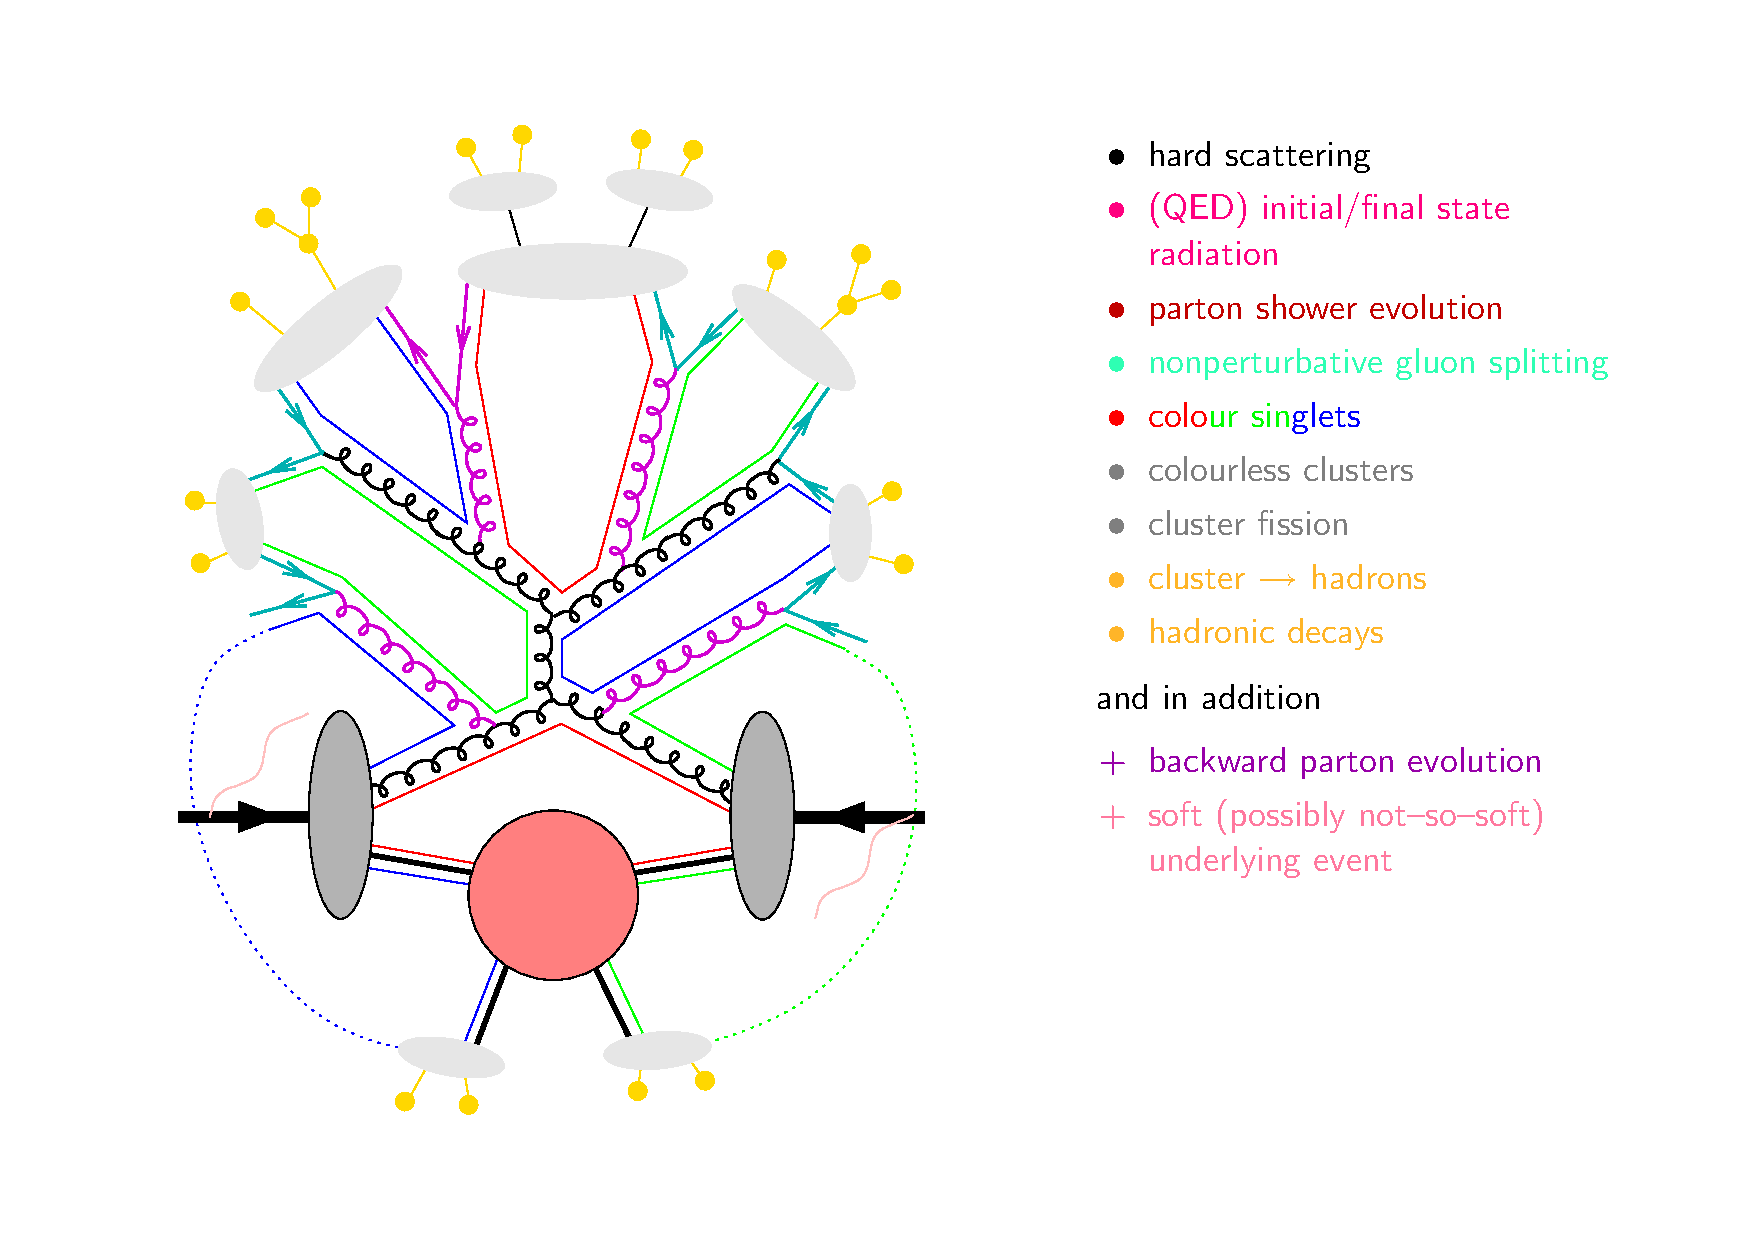
\includegraphics[width=\textwidth]{figures/Zep-soft}
\caption{An illustration of the processes that may surround an interesting event in a proton-proton collision, and the steps required to arrive at a final particle content of that event. In this figure, the dark gray blobs represent the incoming protons and the large red blob represents a hard quark-quark interaction. As illustrated here, the products of such a hard interaction may carry colour charge as well, in which case these products too would need to undergo hadronisation, which, in turn, would show up in the detector as jets. However, since the end product of the process currently under study is photons, which are colourless, that will not be the case here. The upper portion of the figure illustrates the evolution of a secondary gluon interaction, which, though a number of gluon emissions, produces a selection of quark final states that must be gathered into colourless clusters and finally into hadrons. Both stages may undergo further evolution or decay during the process. The final collection of hadrons, which for a single parton interaction will be reasonably well collimated, form a jet of particles in the detector. Similar jet-forming processes may also attach to particles emitted as initial or final state radiation. This figure reproduced from \cite{zep}. For further details on these surrounding processes and their computational representation, see e.g.~\cite{pythman}.
\label{zep}}
\end{figure}

\section{Extended event}
The events produced by the event generator(s) represent the physical process that occurs in the point where two protons interact. Given the limits on our ability to see such interactions, we need to exptend the scope of physical processes in the simulation, to the point where the resulting event information represents something that we might realistically observe with a detector.

The initial and final particle states are fixed in the event generator, however in reality, both initial and final states might easily undergo decay or emission before or after the event occurs, altering the particle content and kinematics of the event. Such initial and final state radiation must be modelled to give an accurate picture of what a detector might see.

Further, final state particles with colour charge will not remain isolated due to colour confinement. These particles will develop a jet of other coloured particles, so that the colour charge becomes obscured to outside observation. The simulation of the process by which colour charged particles combine into colour neutral hadrons is simulated is called hadronisation. Since we are dealing with photons in the final state in the present analysis, this step is not crucial in the events generated to study this process specifically, however $\pi^0$ mesons, one of the major backgrounds to the photon signal, are produced in this way. 

A schematic summary of these processes, along with the steps that the simulation software that models these processes will usually be divided into, is presented in figure~\ref{zep}. In this thesis, the extension of the hard events provided by CalcHEP with these surrounding processes will be carried out in pythia8 \cite{pythia}. Figure~\ref{pythify} illustrates the effect that these surrounding processes have on the distribution of invariant masses.

\begin{figure}[htp]
\centering
\begin{minipage}[b]{.69\textwidth}\hspace{-1.5em}\makebox[0pt][l]{
\noindent\begin{infilsf}
\tiny
\pgfdeclareplotmark{cross} {
\pgfpathmoveto{\pgfpoint{-0.3\pgfplotmarksize}{\pgfplotmarksize}}
\pgfpathlineto{\pgfpoint{+0.3\pgfplotmarksize}{\pgfplotmarksize}}
\pgfpathlineto{\pgfpoint{+0.3\pgfplotmarksize}{0.3\pgfplotmarksize}}
\pgfpathlineto{\pgfpoint{+1\pgfplotmarksize}{0.3\pgfplotmarksize}}
\pgfpathlineto{\pgfpoint{+1\pgfplotmarksize}{-0.3\pgfplotmarksize}}
\pgfpathlineto{\pgfpoint{+0.3\pgfplotmarksize}{-0.3\pgfplotmarksize}}
\pgfpathlineto{\pgfpoint{+0.3\pgfplotmarksize}{-1.\pgfplotmarksize}}
\pgfpathlineto{\pgfpoint{-0.3\pgfplotmarksize}{-1.\pgfplotmarksize}}
\pgfpathlineto{\pgfpoint{-0.3\pgfplotmarksize}{-0.3\pgfplotmarksize}}
\pgfpathlineto{\pgfpoint{-1.\pgfplotmarksize}{-0.3\pgfplotmarksize}}
\pgfpathlineto{\pgfpoint{-1.\pgfplotmarksize}{0.3\pgfplotmarksize}}
\pgfpathlineto{\pgfpoint{-0.3\pgfplotmarksize}{0.3\pgfplotmarksize}}
\pgfpathclose
\pgfusepathqstroke
}
\pgfdeclareplotmark{cross*} {
\pgfpathmoveto{\pgfpoint{-0.3\pgfplotmarksize}{\pgfplotmarksize}}
\pgfpathlineto{\pgfpoint{+0.3\pgfplotmarksize}{\pgfplotmarksize}}
\pgfpathlineto{\pgfpoint{+0.3\pgfplotmarksize}{0.3\pgfplotmarksize}}
\pgfpathlineto{\pgfpoint{+1\pgfplotmarksize}{0.3\pgfplotmarksize}}
\pgfpathlineto{\pgfpoint{+1\pgfplotmarksize}{-0.3\pgfplotmarksize}}
\pgfpathlineto{\pgfpoint{+0.3\pgfplotmarksize}{-0.3\pgfplotmarksize}}
\pgfpathlineto{\pgfpoint{+0.3\pgfplotmarksize}{-1.\pgfplotmarksize}}
\pgfpathlineto{\pgfpoint{-0.3\pgfplotmarksize}{-1.\pgfplotmarksize}}
\pgfpathlineto{\pgfpoint{-0.3\pgfplotmarksize}{-0.3\pgfplotmarksize}}
\pgfpathlineto{\pgfpoint{-1.\pgfplotmarksize}{-0.3\pgfplotmarksize}}
\pgfpathlineto{\pgfpoint{-1.\pgfplotmarksize}{0.3\pgfplotmarksize}}
\pgfpathlineto{\pgfpoint{-0.3\pgfplotmarksize}{0.3\pgfplotmarksize}}
\pgfpathclose
\pgfusepathqfillstroke
}
\pgfdeclareplotmark{newstar} {
\pgfpathmoveto{\pgfqpoint{0pt}{\pgfplotmarksize}}
\pgfpathlineto{\pgfqpointpolar{44}{0.5\pgfplotmarksize}}
\pgfpathlineto{\pgfqpointpolar{18}{\pgfplotmarksize}}
\pgfpathlineto{\pgfqpointpolar{-20}{0.5\pgfplotmarksize}}
\pgfpathlineto{\pgfqpointpolar{-54}{\pgfplotmarksize}}
\pgfpathlineto{\pgfqpointpolar{-90}{0.5\pgfplotmarksize}}
\pgfpathlineto{\pgfqpointpolar{234}{\pgfplotmarksize}}
\pgfpathlineto{\pgfqpointpolar{198}{0.5\pgfplotmarksize}}
\pgfpathlineto{\pgfqpointpolar{162}{\pgfplotmarksize}}
\pgfpathlineto{\pgfqpointpolar{134}{0.5\pgfplotmarksize}}
\pgfpathclose
\pgfusepathqstroke
}
\pgfdeclareplotmark{newstar*} {
\pgfpathmoveto{\pgfqpoint{0pt}{\pgfplotmarksize}}
\pgfpathlineto{\pgfqpointpolar{44}{0.5\pgfplotmarksize}}
\pgfpathlineto{\pgfqpointpolar{18}{\pgfplotmarksize}}
\pgfpathlineto{\pgfqpointpolar{-20}{0.5\pgfplotmarksize}}
\pgfpathlineto{\pgfqpointpolar{-54}{\pgfplotmarksize}}
\pgfpathlineto{\pgfqpointpolar{-90}{0.5\pgfplotmarksize}}
\pgfpathlineto{\pgfqpointpolar{234}{\pgfplotmarksize}}
\pgfpathlineto{\pgfqpointpolar{198}{0.5\pgfplotmarksize}}
\pgfpathlineto{\pgfqpointpolar{162}{\pgfplotmarksize}}
\pgfpathlineto{\pgfqpointpolar{134}{0.5\pgfplotmarksize}}
\pgfpathclose
\pgfusepathqfillstroke
}
\begin{tikzpicture}[x=0.05\textwidth,y=.05\textwidth]

\definecolor{c}{rgb}{0,0,0};
\draw [c] (2,11.8008) -- (2,22.4216) -- (18,22.4216) -- (18,11.8008) -- (2,11.8008);

\definecolor{c}{rgb}{0,0,0};
\draw [c] (2,11.8008) -- (2,22.4216) -- (18,22.4216) -- (18,11.8008) -- (2,11.8008);
\colorlet{c}{kugray!50};
\draw [c] (2.16,22.0847) -- (2.16,22.0869);
\draw [c] (2.16,22.0869) -- (2.16,22.0891);
\draw [c] (2,22.0869) -- (2.16,22.0869);
\draw [c] (2.16,22.0869) -- (2.32,22.0869);
\draw [c] (2.48,20.989) -- (2.48,20.9954);
\draw [c] (2.48,20.9954) -- (2.48,21.0016);
\draw [c] (2.32,20.9954) -- (2.48,20.9954);
\draw [c] (2.48,20.9954) -- (2.64,20.9954);
\draw [c] (2.8,20.2777) -- (2.8,20.2902);
\draw [c] (2.8,20.2902) -- (2.8,20.3024);
\draw [c] (2.64,20.2902) -- (2.8,20.2902);
\draw [c] (2.8,20.2902) -- (2.96,20.2902);
\draw [c] (3.12,19.7357) -- (3.12,19.7568);
\draw [c] (3.12,19.7568) -- (3.12,19.777);
\draw [c] (2.96,19.7568) -- (3.12,19.7568);
\draw [c] (3.12,19.7568) -- (3.28,19.7568);
\draw [c] (3.44,19.2804) -- (3.44,19.313);
\draw [c] (3.44,19.313) -- (3.44,19.3436);
\draw [c] (3.28,19.313) -- (3.44,19.313);
\draw [c] (3.44,19.313) -- (3.6,19.313);
\draw [c] (3.76,18.9425) -- (3.76,18.9876);
\draw [c] (3.76,18.9876) -- (3.76,19.0291);
\draw [c] (3.6,18.9876) -- (3.76,18.9876);
\draw [c] (3.76,18.9876) -- (3.92,18.9876);
\draw [c] (4.08,18.4927) -- (4.08,18.5621);
\draw [c] (4.08,18.5621) -- (4.08,18.6234);
\draw [c] (3.92,18.5621) -- (4.08,18.5621);
\draw [c] (4.08,18.5621) -- (4.24,18.5621);
\draw [c] (4.4,18.1352) -- (4.4,18.2331);
\draw [c] (4.4,18.2331) -- (4.4,18.3154);
\draw [c] (4.24,18.2331) -- (4.4,18.2331);
\draw [c] (4.4,18.2331) -- (4.56,18.2331);
\draw [c] (4.72,17.8253) -- (4.72,17.957);
\draw [c] (4.72,17.957) -- (4.72,18.062);
\draw [c] (4.56,17.957) -- (4.72,17.957);
\draw [c] (4.72,17.957) -- (4.88,17.957);
\draw [c] (5.04,17.7645) -- (5.04,17.8494);
\draw [c] (5.04,17.8494) -- (5.04,17.9225);
\draw [c] (4.88,17.8494) -- (5.04,17.8494);
\draw [c] (5.04,17.8494) -- (5.2,17.8494);
\draw [c] (5.36,17.4837) -- (5.36,17.4878);
\draw [c] (5.36,17.4878) -- (5.36,17.4919);
\draw [c] (5.2,17.4878) -- (5.36,17.4878);
\draw [c] (5.36,17.4878) -- (5.52,17.4878);
\draw [c] (5.68,17.2475) -- (5.68,17.2526);
\draw [c] (5.68,17.2526) -- (5.68,17.2577);
\draw [c] (5.52,17.2526) -- (5.68,17.2526);
\draw [c] (5.68,17.2526) -- (5.84,17.2526);
\draw [c] (6,16.9982) -- (6,17.0047);
\draw [c] (6,17.0047) -- (6,17.0112);
\draw [c] (5.84,17.0047) -- (6,17.0047);
\draw [c] (6,17.0047) -- (6.16,17.0047);
\draw [c] (6.32,16.7792) -- (6.32,16.7873);
\draw [c] (6.32,16.7873) -- (6.32,16.7952);
\draw [c] (6.16,16.7873) -- (6.32,16.7873);
\draw [c] (6.32,16.7873) -- (6.48,16.7873);
\draw [c] (6.64,16.5651) -- (6.64,16.575);
\draw [c] (6.64,16.575) -- (6.64,16.5847);
\draw [c] (6.48,16.575) -- (6.64,16.575);
\draw [c] (6.64,16.575) -- (6.8,16.575);
\draw [c] (6.96,16.3657) -- (6.96,16.3776);
\draw [c] (6.96,16.3776) -- (6.96,16.3893);
\draw [c] (6.8,16.3776) -- (6.96,16.3776);
\draw [c] (6.96,16.3776) -- (7.12,16.3776);
\draw [c] (7.28,16.1641) -- (7.28,16.1786);
\draw [c] (7.28,16.1786) -- (7.28,16.1927);
\draw [c] (7.12,16.1786) -- (7.28,16.1786);
\draw [c] (7.28,16.1786) -- (7.44,16.1786);
\draw [c] (7.6,15.9868) -- (7.6,16.004);
\draw [c] (7.6,16.004) -- (7.6,16.0206);
\draw [c] (7.44,16.004) -- (7.6,16.004);
\draw [c] (7.6,16.004) -- (7.76,16.004);
\draw [c] (7.92,15.7677) -- (7.92,15.7889);
\draw [c] (7.92,15.7889) -- (7.92,15.8093);
\draw [c] (7.76,15.7889) -- (7.92,15.7889);
\draw [c] (7.92,15.7889) -- (8.08,15.7889);
\draw [c] (8.24,15.4855) -- (8.24,15.5133);
\draw [c] (8.24,15.5133) -- (8.24,15.5398);
\draw [c] (8.08,15.5133) -- (8.24,15.5133);
\draw [c] (8.24,15.5133) -- (8.4,15.5133);
\draw [c] (8.56,15.2517) -- (8.56,15.2866);
\draw [c] (8.56,15.2866) -- (8.56,15.3193);
\draw [c] (8.4,15.2866) -- (8.56,15.2866);
\draw [c] (8.56,15.2866) -- (8.72,15.2866);
\draw [c] (8.88,14.9685) -- (8.88,15.0142);
\draw [c] (8.88,15.0142) -- (8.88,15.0563);
\draw [c] (8.72,15.0142) -- (8.88,15.0142);
\draw [c] (8.88,15.0142) -- (9.04,15.0142);
\draw [c] (9.2,14.9072) -- (9.2,14.9557);
\draw [c] (9.2,14.9557) -- (9.2,15.0001);
\draw [c] (9.04,14.9557) -- (9.2,14.9557);
\draw [c] (9.2,14.9557) -- (9.36,14.9557);
\draw [c] (9.52,14.6847) -- (9.52,14.7448);
\draw [c] (9.52,14.7448) -- (9.52,14.7987);
\draw [c] (9.36,14.7448) -- (9.52,14.7448);
\draw [c] (9.52,14.7448) -- (9.68,14.7448);
\draw [c] (9.84,14.3956) -- (9.84,14.4749);
\draw [c] (9.84,14.4749) -- (9.84,14.5437);
\draw [c] (9.68,14.4749) -- (9.84,14.4749);
\draw [c] (9.84,14.4749) -- (10,14.4749);
\draw [c] (10.16,14.24) -- (10.16,14.3321);
\draw [c] (10.16,14.3321) -- (10.16,14.4103);
\draw [c] (10,14.3321) -- (10.16,14.3321);
\draw [c] (10.16,14.3321) -- (10.32,14.3321);
\draw [c] (10.48,13.9492) -- (10.48,14.0709);
\draw [c] (10.48,14.0709) -- (10.48,14.1694);
\draw [c] (10.32,14.0709) -- (10.48,14.0709);
\draw [c] (10.48,14.0709) -- (10.64,14.0709);
\draw [c] (10.8,13.923) -- (10.8,14.0478);
\draw [c] (10.8,14.0478) -- (10.8,14.1483);
\draw [c] (10.64,14.0478) -- (10.8,14.0478);
\draw [c] (10.8,14.0478) -- (10.96,14.0478);
\draw [c] (11.12,13.6051) -- (11.12,13.7741);
\draw [c] (11.12,13.7741) -- (11.12,13.9014);
\draw [c] (10.96,13.7741) -- (11.12,13.7741);
\draw [c] (11.12,13.7741) -- (11.28,13.7741);
\draw [c] (11.44,13.5552) -- (11.44,13.7324);
\draw [c] (11.44,13.7324) -- (11.44,13.8644);
\draw [c] (11.28,13.7324) -- (11.44,13.7324);
\draw [c] (11.44,13.7324) -- (11.6,13.7324);
\draw [c] (11.76,13.5005) -- (11.76,13.6872);
\draw [c] (11.76,13.6872) -- (11.76,13.8243);
\draw [c] (11.6,13.6872) -- (11.76,13.6872);
\draw [c] (11.76,13.6872) -- (11.92,13.6872);
\draw [c] (12.08,12.8003) -- (12.08,13.1609);
\draw [c] (12.08,13.1609) -- (12.08,13.3718);
\draw [c] (11.92,13.1609) -- (12.08,13.1609);
\draw [c] (12.08,13.1609) -- (12.24,13.1609);
\draw [c] (12.4,13.5005) -- (12.4,13.6872);
\draw [c] (12.4,13.6872) -- (12.4,13.8243);
\draw [c] (12.24,13.6872) -- (12.4,13.6872);
\draw [c] (12.4,13.6872) -- (12.56,13.6872);
\draw [c] (12.72,11.8008) -- (12.72,12.4397);
\draw [c] (12.72,12.4397) -- (12.72,12.8003);
\draw [c] (12.56,12.4397) -- (12.72,12.4397);
\draw [c] (12.72,12.4397) -- (12.88,12.4397);
\draw [c] (13.04,11.8008) -- (13.04,12.4397);
\draw [c] (13.04,12.4397) -- (13.04,12.8003);
\draw [c] (12.88,12.4397) -- (13.04,12.4397);
\draw [c] (13.04,12.4397) -- (13.2,12.4397);
\draw [c] (13.36,11.8008) -- (13.36,12.4397);
\draw [c] (13.36,12.4397) -- (13.36,12.8003);
\draw [c] (13.2,12.4397) -- (13.36,12.4397);
\draw [c] (13.36,12.4397) -- (13.52,12.4397);
\draw [c] (13.68,12.1614) -- (13.68,12.8003);
\draw [c] (13.68,12.8003) -- (13.68,13.0785);
\draw [c] (13.52,12.8003) -- (13.68,12.8003);
\draw [c] (13.68,12.8003) -- (13.84,12.8003);
\draw [c] (14,11.8008) -- (14,12.4397);
\draw [c] (14,12.4397) -- (14,12.8003);
\draw [c] (13.84,12.4397) -- (14,12.4397);
\draw [c] (14,12.4397) -- (14.16,12.4397);
\draw [c] (14.32,11.8008) -- (14.32,12.4397);
\draw [c] (14.32,12.4397) -- (14.32,12.8003);
\draw [c] (14.16,12.4397) -- (14.32,12.4397);
\draw [c] (14.32,12.4397) -- (14.48,12.4397);
\draw [c] (14.64,11.8008) -- (14.64,12.4397);
\draw [c] (14.64,12.4397) -- (14.64,12.8003);
\draw [c] (14.48,12.4397) -- (14.64,12.4397);
\draw [c] (14.64,12.4397) -- (14.8,12.4397);
\draw [c] (15.28,11.8008) -- (15.28,12.4397);
\draw [c] (15.28,12.4397) -- (15.28,12.8003);
\draw [c] (15.12,12.4397) -- (15.28,12.4397);
\draw [c] (15.28,12.4397) -- (15.44,12.4397);
\definecolor{c}{rgb}{0,0,0};
\draw [c] (2,11.8008) -- (18,11.8008);
\draw [c] (3.30612,12.084) -- (3.30612,11.8008);
\draw [c] (3.63265,11.9424) -- (3.63265,11.8008);
\draw [c] (3.95918,11.9424) -- (3.95918,11.8008);
\draw [c] (4.28571,11.9424) -- (4.28571,11.8008);
\draw [c] (4.61225,11.9424) -- (4.61225,11.8008);
\draw [c] (4.93878,12.084) -- (4.93878,11.8008);
\draw [c] (5.26531,11.9424) -- (5.26531,11.8008);
\draw [c] (5.59184,11.9424) -- (5.59184,11.8008);
\draw [c] (5.91837,11.9424) -- (5.91837,11.8008);
\draw [c] (6.2449,11.9424) -- (6.2449,11.8008);
\draw [c] (6.57143,12.084) -- (6.57143,11.8008);
\draw [c] (6.89796,11.9424) -- (6.89796,11.8008);
\draw [c] (7.22449,11.9424) -- (7.22449,11.8008);
\draw [c] (7.55102,11.9424) -- (7.55102,11.8008);
\draw [c] (7.87755,11.9424) -- (7.87755,11.8008);
\draw [c] (8.20408,12.084) -- (8.20408,11.8008);
\draw [c] (8.53061,11.9424) -- (8.53061,11.8008);
\draw [c] (8.85714,11.9424) -- (8.85714,11.8008);
\draw [c] (9.18367,11.9424) -- (9.18367,11.8008);
\draw [c] (9.5102,11.9424) -- (9.5102,11.8008);
\draw [c] (9.83673,12.084) -- (9.83673,11.8008);
\draw [c] (10.1633,11.9424) -- (10.1633,11.8008);
\draw [c] (10.4898,11.9424) -- (10.4898,11.8008);
\draw [c] (10.8163,11.9424) -- (10.8163,11.8008);
\draw [c] (11.1429,11.9424) -- (11.1429,11.8008);
\draw [c] (11.4694,12.084) -- (11.4694,11.8008);
\draw [c] (11.7959,11.9424) -- (11.7959,11.8008);
\draw [c] (12.1224,11.9424) -- (12.1224,11.8008);
\draw [c] (12.449,11.9424) -- (12.449,11.8008);
\draw [c] (12.7755,11.9424) -- (12.7755,11.8008);
\draw [c] (13.102,12.084) -- (13.102,11.8008);
\draw [c] (13.4286,11.9424) -- (13.4286,11.8008);
\draw [c] (13.7551,11.9424) -- (13.7551,11.8008);
\draw [c] (14.0816,11.9424) -- (14.0816,11.8008);
\draw [c] (14.4082,11.9424) -- (14.4082,11.8008);
\draw [c] (14.7347,12.084) -- (14.7347,11.8008);
\draw [c] (15.0612,11.9424) -- (15.0612,11.8008);
\draw [c] (15.3878,11.9424) -- (15.3878,11.8008);
\draw [c] (15.7143,11.9424) -- (15.7143,11.8008);
\draw [c] (16.0408,11.9424) -- (16.0408,11.8008);
\draw [c] (16.3673,12.084) -- (16.3673,11.8008);
\draw [c] (16.6939,11.9424) -- (16.6939,11.8008);
\draw [c] (17.0204,11.9424) -- (17.0204,11.8008);
\draw [c] (17.3469,11.9424) -- (17.3469,11.8008);
\draw [c] (17.6735,11.9424) -- (17.6735,11.8008);
\draw [c] (18,12.084) -- (18,11.8008);
\draw [c] (3.30612,12.084) -- (3.30612,11.8008);
\draw [c] (2.97959,11.9424) -- (2.97959,11.8008);
\draw [c] (2.65306,11.9424) -- (2.65306,11.8008);
\draw [c] (2.32653,11.9424) -- (2.32653,11.8008);

\draw [c] (2,11.8008) -- (2,22.4216);
\draw [anchor= east] (0.1,22.4216) node[ rotate=90]{$\di\sigma/\di M_{\gamma\gamma}$ [pb/GeV]};
\draw [c] (2.27,11.8185) -- (2,11.8185);
\draw [c] (2.27,11.8986) -- (2,11.8986);
\draw [c] (2.27,11.9681) -- (2,11.9681);
\draw [c] (2.27,12.0294) -- (2,12.0294);
\draw [c] (2.54,12.0842) -- (2,12.0842);
\draw [anchor= east] (1.844,12.0842) node[ rotate=0]{$10^{-10}$};
\draw [c] (2.27,12.4448) -- (2,12.4448);
\draw [c] (2.27,12.6558) -- (2,12.6558);
\draw [c] (2.27,12.8054) -- (2,12.8054);
\draw [c] (2.27,12.9215) -- (2,12.9215);
\draw [c] (2.27,13.0164) -- (2,13.0164);
\draw [c] (2.27,13.0966) -- (2,13.0966);
\draw [c] (2.27,13.166) -- (2,13.166);
\draw [c] (2.27,13.2273) -- (2,13.2273);
\draw [c] (2.54,13.2821) -- (2,13.2821);
\draw [anchor= east] (1.844,13.2821) node[ rotate=0]{$10^{-9}$};
\draw [c] (2.27,13.6427) -- (2,13.6427);
\draw [c] (2.27,13.8537) -- (2,13.8537);
\draw [c] (2.27,14.0033) -- (2,14.0033);
\draw [c] (2.27,14.1194) -- (2,14.1194);
\draw [c] (2.27,14.2143) -- (2,14.2143);
\draw [c] (2.27,14.2945) -- (2,14.2945);
\draw [c] (2.27,14.364) -- (2,14.364);
\draw [c] (2.27,14.4252) -- (2,14.4252);
\draw [c] (2.54,14.48) -- (2,14.48);
\draw [anchor= east] (1.844,14.48) node[ rotate=0]{$10^{-8}$};
\draw [c] (2.27,14.8407) -- (2,14.8407);
\draw [c] (2.27,15.0516) -- (2,15.0516);
\draw [c] (2.27,15.2013) -- (2,15.2013);
\draw [c] (2.27,15.3174) -- (2,15.3174);
\draw [c] (2.27,15.4122) -- (2,15.4122);
\draw [c] (2.27,15.4924) -- (2,15.4924);
\draw [c] (2.27,15.5619) -- (2,15.5619);
\draw [c] (2.27,15.6231) -- (2,15.6231);
\draw [c] (2.54,15.678) -- (2,15.678);
\draw [anchor= east] (1.844,15.678) node[ rotate=0]{$10^{-7}$};
\draw [c] (2.27,16.0386) -- (2,16.0386);
\draw [c] (2.27,16.2495) -- (2,16.2495);
\draw [c] (2.27,16.3992) -- (2,16.3992);
\draw [c] (2.27,16.5153) -- (2,16.5153);
\draw [c] (2.27,16.6101) -- (2,16.6101);
\draw [c] (2.27,16.6903) -- (2,16.6903);
\draw [c] (2.27,16.7598) -- (2,16.7598);
\draw [c] (2.27,16.8211) -- (2,16.8211);
\draw [c] (2.54,16.8759) -- (2,16.8759);
\draw [anchor= east] (1.844,16.8759) node[ rotate=0]{$10^{-6}$};
\draw [c] (2.27,17.2365) -- (2,17.2365);
\draw [c] (2.27,17.4474) -- (2,17.4474);
\draw [c] (2.27,17.5971) -- (2,17.5971);
\draw [c] (2.27,17.7132) -- (2,17.7132);
\draw [c] (2.27,17.808) -- (2,17.808);
\draw [c] (2.27,17.8882) -- (2,17.8882);
\draw [c] (2.27,17.9577) -- (2,17.9577);
\draw [c] (2.27,18.019) -- (2,18.019);
\draw [c] (2.54,18.0738) -- (2,18.0738);
\draw [anchor= east] (1.844,18.0738) node[ rotate=0]{$10^{-5}$};
\draw [c] (2.27,18.4344) -- (2,18.4344);
\draw [c] (2.27,18.6453) -- (2,18.6453);
\draw [c] (2.27,18.795) -- (2,18.795);
\draw [c] (2.27,18.9111) -- (2,18.9111);
\draw [c] (2.27,19.006) -- (2,19.006);
\draw [c] (2.27,19.0861) -- (2,19.0861);
\draw [c] (2.27,19.1556) -- (2,19.1556);
\draw [c] (2.27,19.2169) -- (2,19.2169);
\draw [c] (2.54,19.2717) -- (2,19.2717);
\draw [anchor= east] (1.844,19.2717) node[ rotate=0]{$10^{-4}$};
\draw [c] (2.27,19.6323) -- (2,19.6323);
\draw [c] (2.27,19.8433) -- (2,19.8433);
\draw [c] (2.27,19.9929) -- (2,19.9929);
\draw [c] (2.27,20.109) -- (2,20.109);
\draw [c] (2.27,20.2039) -- (2,20.2039);
\draw [c] (2.27,20.2841) -- (2,20.2841);
\draw [c] (2.27,20.3535) -- (2,20.3535);
\draw [c] (2.27,20.4148) -- (2,20.4148);
\draw [c] (2.54,20.4696) -- (2,20.4696);
\draw [anchor= east] (1.844,20.4696) node[ rotate=0]{$10^{-3}$};
\draw [c] (2.27,20.8302) -- (2,20.8302);
\draw [c] (2.27,21.0412) -- (2,21.0412);
\draw [c] (2.27,21.1908) -- (2,21.1908);
\draw [c] (2.27,21.3069) -- (2,21.3069);
\draw [c] (2.27,21.4018) -- (2,21.4018);
\draw [c] (2.27,21.482) -- (2,21.482);
\draw [c] (2.27,21.5515) -- (2,21.5515);
\draw [c] (2.27,21.6127) -- (2,21.6127);
\draw [c] (2.54,21.6675) -- (2,21.6675);
\draw [anchor= east] (1.844,21.6675) node[ rotate=0]{$10^{-2}$};
\draw [c] (2.27,22.0282) -- (2,22.0282);
\draw [c] (2.27,22.2391) -- (2,22.2391);
\draw [c] (2.27,22.3888) -- (2,22.3888);
\colorlet{c}{kugray};
\draw [c] (2.16,21.9886) -- (2.16,21.9911);
\draw [c] (2.16,21.9911) -- (2.16,21.9935);
\draw [c] (2,21.9911) -- (2.16,21.9911);
\draw [c] (2.16,21.9911) -- (2.32,21.9911);
\draw [c] (2.48,20.8999) -- (2.48,20.9067);
\draw [c] (2.48,20.9067) -- (2.48,20.9135);
\draw [c] (2.32,20.9067) -- (2.48,20.9067);
\draw [c] (2.48,20.9067) -- (2.64,20.9067);
\draw [c] (2.8,20.1651) -- (2.8,20.179);
\draw [c] (2.8,20.179) -- (2.8,20.1926);
\draw [c] (2.64,20.179) -- (2.8,20.179);
\draw [c] (2.8,20.179) -- (2.96,20.179);
\draw [c] (3.12,19.6256) -- (3.12,19.649);
\draw [c] (3.12,19.649) -- (3.12,19.6714);
\draw [c] (2.96,19.649) -- (3.12,19.649);
\draw [c] (3.12,19.649) -- (3.28,19.649);
\draw [c] (3.44,19.2037) -- (3.44,19.2388);
\draw [c] (3.44,19.2388) -- (3.44,19.2717);
\draw [c] (3.28,19.2388) -- (3.44,19.2388);
\draw [c] (3.44,19.2388) -- (3.6,19.2388);
\draw [c] (3.76,18.8394) -- (3.76,18.8892);
\draw [c] (3.76,18.8892) -- (3.76,18.9346);
\draw [c] (3.6,18.8892) -- (3.76,18.8892);
\draw [c] (3.76,18.8892) -- (3.92,18.8892);
\draw [c] (4.08,18.3977) -- (4.08,18.4738);
\draw [c] (4.08,18.4738) -- (4.08,18.5401);
\draw [c] (3.92,18.4738) -- (4.08,18.4738);
\draw [c] (4.08,18.4738) -- (4.24,18.4738);
\draw [c] (4.4,18.0231) -- (4.4,18.1321);
\draw [c] (4.4,18.1321) -- (4.4,18.2221);
\draw [c] (4.24,18.1321) -- (4.4,18.1321);
\draw [c] (4.4,18.1321) -- (4.56,18.1321);
\draw [c] (4.72,17.5639) -- (4.72,17.7329);
\draw [c] (4.72,17.7329) -- (4.72,17.8603);
\draw [c] (4.56,17.7329) -- (4.72,17.7329);
\draw [c] (4.72,17.7329) -- (4.88,17.7329);
\draw [c] (5.04,17.6487) -- (5.04,17.7446);
\draw [c] (5.04,17.7446) -- (5.04,17.8255);
\draw [c] (4.88,17.7446) -- (5.04,17.7446);
\draw [c] (5.04,17.7446) -- (5.2,17.7446);
\draw [c] (5.36,17.3748) -- (5.36,17.3793);
\draw [c] (5.36,17.3793) -- (5.36,17.3838);
\draw [c] (5.2,17.3793) -- (5.36,17.3793);
\draw [c] (5.36,17.3793) -- (5.52,17.3793);
\draw [c] (5.68,17.1419) -- (5.68,17.1476);
\draw [c] (5.68,17.1476) -- (5.68,17.1532);
\draw [c] (5.52,17.1476) -- (5.68,17.1476);
\draw [c] (5.68,17.1476) -- (5.84,17.1476);
\draw [c] (6,16.8903) -- (6,16.8975);
\draw [c] (6,16.8975) -- (6,16.9046);
\draw [c] (5.84,16.8975) -- (6,16.8975);
\draw [c] (6,16.8975) -- (6.16,16.8975);
\draw [c] (6.32,16.6718) -- (6.32,16.6807);
\draw [c] (6.32,16.6807) -- (6.32,16.6894);
\draw [c] (6.16,16.6807) -- (6.32,16.6807);
\draw [c] (6.32,16.6807) -- (6.48,16.6807);
\draw [c] (6.64,16.4482) -- (6.64,16.4592);
\draw [c] (6.64,16.4592) -- (6.64,16.47);
\draw [c] (6.48,16.4592) -- (6.64,16.4592);
\draw [c] (6.64,16.4592) -- (6.8,16.4592);
\draw [c] (6.96,16.2518) -- (6.96,16.2651);
\draw [c] (6.96,16.2651) -- (6.96,16.2781);
\draw [c] (6.8,16.2651) -- (6.96,16.2651);
\draw [c] (6.96,16.2651) -- (7.12,16.2651);
\draw [c] (7.28,16.043) -- (7.28,16.0593);
\draw [c] (7.28,16.0593) -- (7.28,16.0751);
\draw [c] (7.12,16.0593) -- (7.28,16.0593);
\draw [c] (7.28,16.0593) -- (7.44,16.0593);
\draw [c] (7.6,15.8872) -- (7.6,15.9061);
\draw [c] (7.6,15.9061) -- (7.6,15.9244);
\draw [c] (7.44,15.9061) -- (7.6,15.9061);
\draw [c] (7.6,15.9061) -- (7.76,15.9061);
\draw [c] (7.92,15.6564) -- (7.92,15.68);
\draw [c] (7.92,15.68) -- (7.92,15.7026);
\draw [c] (7.76,15.68) -- (7.92,15.68);
\draw [c] (7.92,15.68) -- (8.08,15.68);
\draw [c] (8.24,15.3725) -- (8.24,15.4036);
\draw [c] (8.24,15.4036) -- (8.24,15.4329);
\draw [c] (8.08,15.4036) -- (8.24,15.4036);
\draw [c] (8.24,15.4036) -- (8.4,15.4036);
\draw [c] (8.56,15.1099) -- (8.56,15.1499);
\draw [c] (8.56,15.1499) -- (8.56,15.187);
\draw [c] (8.4,15.1499) -- (8.56,15.1499);
\draw [c] (8.56,15.1499) -- (8.72,15.1499);
\draw [c] (8.88,14.862) -- (8.88,14.9127);
\draw [c] (8.88,14.9127) -- (8.88,14.9589);
\draw [c] (8.72,14.9127) -- (8.88,14.9127);
\draw [c] (8.88,14.9127) -- (9.04,14.9127);
\draw [c] (9.2,14.8126) -- (9.2,14.8658);
\draw [c] (9.2,14.8658) -- (9.2,14.914);
\draw [c] (9.04,14.8658) -- (9.2,14.8658);
\draw [c] (9.2,14.8658) -- (9.36,14.8658);
\draw [c] (9.52,14.5837) -- (9.52,14.6499);
\draw [c] (9.52,14.6499) -- (9.52,14.7087);
\draw [c] (9.36,14.6499) -- (9.52,14.6499);
\draw [c] (9.52,14.6499) -- (9.68,14.6499);
\draw [c] (9.84,14.2548) -- (9.84,14.3456);
\draw [c] (9.84,14.3456) -- (9.84,14.4229);
\draw [c] (9.68,14.3456) -- (9.84,14.3456);
\draw [c] (9.84,14.3456) -- (10,14.3456);
\draw [c] (10.16,14.1042) -- (10.16,14.2091);
\draw [c] (10.16,14.2091) -- (10.16,14.2964);
\draw [c] (10,14.2091) -- (10.16,14.2091);
\draw [c] (10.16,14.2091) -- (10.32,14.2091);
\draw [c] (10.48,13.7691) -- (10.48,13.9136);
\draw [c] (10.48,13.9136) -- (10.48,14.0266);
\draw [c] (10.32,13.9136) -- (10.48,13.9136);
\draw [c] (10.48,13.9136) -- (10.64,13.9136);
\draw [c] (10.8,13.7691) -- (10.8,13.9136);
\draw [c] (10.8,13.9136) -- (10.8,14.0266);
\draw [c] (10.64,13.9136) -- (10.8,13.9136);
\draw [c] (10.8,13.9136) -- (10.96,13.9136);
\draw [c] (11.12,13.5005) -- (11.12,13.6872);
\draw [c] (11.12,13.6872) -- (11.12,13.8243);
\draw [c] (10.96,13.6872) -- (11.12,13.6872);
\draw [c] (11.12,13.6872) -- (11.28,13.6872);
\draw [c] (11.44,13.4398) -- (11.44,13.6376);
\draw [c] (11.44,13.6376) -- (11.44,13.7805);
\draw [c] (11.28,13.6376) -- (11.44,13.6376);
\draw [c] (11.44,13.6376) -- (11.6,13.6376);
\draw [c] (11.76,13.3718) -- (11.76,13.5828);
\draw [c] (11.76,13.5828) -- (11.76,13.7324);
\draw [c] (11.6,13.5828) -- (11.76,13.5828);
\draw [c] (11.76,13.5828) -- (11.92,13.5828);
\draw [c] (12.08,12.1614) -- (12.08,12.8003);
\draw [c] (12.08,12.8003) -- (12.08,13.0785);
\draw [c] (11.92,12.8003) -- (12.08,12.8003);
\draw [c] (12.08,12.8003) -- (12.24,12.8003);
\draw [c] (12.4,13.4398) -- (12.4,13.6376);
\draw [c] (12.4,13.6376) -- (12.4,13.7805);
\draw [c] (12.24,13.6376) -- (12.4,13.6376);
\draw [c] (12.4,13.6376) -- (12.56,13.6376);
\draw [c] (13.04,11.8008) -- (13.04,12.4397);
\draw [c] (13.04,12.4397) -- (13.04,12.8003);
\draw [c] (12.88,12.4397) -- (13.04,12.4397);
\draw [c] (13.04,12.4397) -- (13.2,12.4397);
\draw [c] (13.36,11.8008) -- (13.36,12.4397);
\draw [c] (13.36,12.4397) -- (13.36,12.8003);
\draw [c] (13.2,12.4397) -- (13.36,12.4397);
\draw [c] (13.36,12.4397) -- (13.52,12.4397);
\draw [c] (13.68,11.8008) -- (13.68,12.4397);
\draw [c] (13.68,12.4397) -- (13.68,12.8003);
\draw [c] (13.52,12.4397) -- (13.68,12.4397);
\draw [c] (13.68,12.4397) -- (13.84,12.4397);
\colorlet{c}{natgreen!50};
\draw [c] (2.16,22.0854) -- (2.16,22.0876);
\draw [c] (2.16,22.0876) -- (2.16,22.0898);
\draw [c] (2,22.0876) -- (2.16,22.0876);
\draw [c] (2.16,22.0876) -- (2.32,22.0876);
\draw [c] (2.48,21.0058) -- (2.48,21.012);
\draw [c] (2.48,21.012) -- (2.48,21.0181);
\draw [c] (2.32,21.012) -- (2.48,21.012);
\draw [c] (2.48,21.012) -- (2.64,21.012);
\draw [c] (2.8,20.2599) -- (2.8,20.2726);
\draw [c] (2.8,20.2726) -- (2.8,20.2851);
\draw [c] (2.64,20.2726) -- (2.8,20.2726);
\draw [c] (2.8,20.2726) -- (2.96,20.2726);
\draw [c] (3.12,19.7099) -- (3.12,19.7315);
\draw [c] (3.12,19.7315) -- (3.12,19.7522);
\draw [c] (2.96,19.7315) -- (3.12,19.7315);
\draw [c] (3.12,19.7315) -- (3.28,19.7315);
\draw [c] (3.44,19.3211) -- (3.44,19.3525);
\draw [c] (3.44,19.3525) -- (3.44,19.3821);
\draw [c] (3.28,19.3525) -- (3.44,19.3525);
\draw [c] (3.44,19.3525) -- (3.6,19.3525);
\draw [c] (3.76,18.928) -- (3.76,18.9738);
\draw [c] (3.76,18.9738) -- (3.76,19.0158);
\draw [c] (3.6,18.9738) -- (3.76,18.9738);
\draw [c] (3.76,18.9738) -- (3.92,18.9738);
\draw [c] (4.08,18.5665) -- (4.08,18.6313);
\draw [c] (4.08,18.6313) -- (4.08,18.6889);
\draw [c] (3.92,18.6313) -- (4.08,18.6313);
\draw [c] (4.08,18.6313) -- (4.24,18.6313);
\draw [c] (4.4,18.2956) -- (4.4,18.3796);
\draw [c] (4.4,18.3796) -- (4.4,18.4519);
\draw [c] (4.24,18.3796) -- (4.4,18.3796);
\draw [c] (4.4,18.3796) -- (4.56,18.3796);
\draw [c] (4.72,18.0441) -- (4.72,18.151);
\draw [c] (4.72,18.151) -- (4.72,18.2396);
\draw [c] (4.56,18.151) -- (4.72,18.151);
\draw [c] (4.72,18.151) -- (4.88,18.151);
\draw [c] (5.04,17.8055) -- (5.04,17.8627);
\draw [c] (5.04,17.8627) -- (5.04,17.9143);
\draw [c] (4.88,17.8627) -- (5.04,17.8627);
\draw [c] (5.04,17.8627) -- (5.2,17.8627);
\draw [c] (5.36,17.6929) -- (5.36,17.6978);
\draw [c] (5.36,17.6978) -- (5.36,17.7026);
\draw [c] (5.2,17.6978) -- (5.36,17.6978);
\draw [c] (5.36,17.6978) -- (5.52,17.6978);
\draw [c] (5.68,17.5229) -- (5.68,17.5286);
\draw [c] (5.68,17.5286) -- (5.68,17.5343);
\draw [c] (5.52,17.5286) -- (5.68,17.5286);
\draw [c] (5.68,17.5286) -- (5.84,17.5286);
\draw [c] (6,17.3746) -- (6,17.3812);
\draw [c] (6,17.3812) -- (6,17.3877);
\draw [c] (5.84,17.3812) -- (6,17.3812);
\draw [c] (6,17.3812) -- (6.16,17.3812);
\draw [c] (6.32,17.2692) -- (6.32,17.2765);
\draw [c] (6.32,17.2765) -- (6.32,17.2837);
\draw [c] (6.16,17.2765) -- (6.32,17.2765);
\draw [c] (6.32,17.2765) -- (6.48,17.2765);
\draw [c] (6.64,17.1541) -- (6.64,17.1623);
\draw [c] (6.64,17.1623) -- (6.64,17.1703);
\draw [c] (6.48,17.1623) -- (6.64,17.1623);
\draw [c] (6.64,17.1623) -- (6.8,17.1623);
\draw [c] (6.96,17.0606) -- (6.96,17.0695);
\draw [c] (6.96,17.0695) -- (6.96,17.0783);
\draw [c] (6.8,17.0695) -- (6.96,17.0695);
\draw [c] (6.96,17.0695) -- (7.12,17.0695);
\draw [c] (7.28,16.9827) -- (7.28,16.9923);
\draw [c] (7.28,16.9923) -- (7.28,17.0018);
\draw [c] (7.12,16.9923) -- (7.28,16.9923);
\draw [c] (7.28,16.9923) -- (7.44,16.9923);
\draw [c] (7.6,16.9271) -- (7.6,16.9372);
\draw [c] (7.6,16.9372) -- (7.6,16.9472);
\draw [c] (7.44,16.9372) -- (7.6,16.9372);
\draw [c] (7.6,16.9372) -- (7.76,16.9372);
\draw [c] (7.92,16.8537) -- (7.92,16.8646);
\draw [c] (7.92,16.8646) -- (7.92,16.8752);
\draw [c] (7.76,16.8646) -- (7.92,16.8646);
\draw [c] (7.92,16.8646) -- (8.08,16.8646);
\draw [c] (8.24,16.8089) -- (8.24,16.8203);
\draw [c] (8.24,16.8203) -- (8.24,16.8314);
\draw [c] (8.08,16.8203) -- (8.24,16.8203);
\draw [c] (8.24,16.8203) -- (8.4,16.8203);
\draw [c] (8.56,16.7645) -- (8.56,16.7764);
\draw [c] (8.56,16.7764) -- (8.56,16.788);
\draw [c] (8.4,16.7764) -- (8.56,16.7764);
\draw [c] (8.56,16.7764) -- (8.72,16.7764);
\draw [c] (8.88,16.7259) -- (8.88,16.7382);
\draw [c] (8.88,16.7382) -- (8.88,16.7502);
\draw [c] (8.72,16.7382) -- (8.88,16.7382);
\draw [c] (8.88,16.7382) -- (9.04,16.7382);
\draw [c] (9.2,16.6876) -- (9.2,16.7004);
\draw [c] (9.2,16.7004) -- (9.2,16.7129);
\draw [c] (9.04,16.7004) -- (9.2,16.7004);
\draw [c] (9.2,16.7004) -- (9.36,16.7004);
\draw [c] (9.52,16.6177) -- (9.52,16.6314);
\draw [c] (9.52,16.6314) -- (9.52,16.6447);
\draw [c] (9.36,16.6314) -- (9.52,16.6314);
\draw [c] (9.52,16.6314) -- (9.68,16.6314);
\draw [c] (9.84,16.5889) -- (9.84,16.603);
\draw [c] (9.84,16.603) -- (9.84,16.6167);
\draw [c] (9.68,16.603) -- (9.84,16.603);
\draw [c] (9.84,16.603) -- (10,16.603);
\draw [c] (10.16,16.5341) -- (10.16,16.5489);
\draw [c] (10.16,16.5489) -- (10.16,16.5633);
\draw [c] (10,16.5489) -- (10.16,16.5489);
\draw [c] (10.16,16.5489) -- (10.32,16.5489);
\draw [c] (10.48,16.4921) -- (10.48,16.5075);
\draw [c] (10.48,16.5075) -- (10.48,16.5225);
\draw [c] (10.32,16.5075) -- (10.48,16.5075);
\draw [c] (10.48,16.5075) -- (10.64,16.5075);
\draw [c] (10.8,16.4375) -- (10.8,16.4538);
\draw [c] (10.8,16.4538) -- (10.8,16.4696);
\draw [c] (10.64,16.4538) -- (10.8,16.4538);
\draw [c] (10.8,16.4538) -- (10.96,16.4538);
\draw [c] (11.12,16.3965) -- (11.12,16.4134);
\draw [c] (11.12,16.4134) -- (11.12,16.4298);
\draw [c] (10.96,16.4134) -- (11.12,16.4134);
\draw [c] (11.12,16.4134) -- (11.28,16.4134);
\draw [c] (11.44,16.3364) -- (11.44,16.3543);
\draw [c] (11.44,16.3543) -- (11.44,16.3716);
\draw [c] (11.28,16.3543) -- (11.44,16.3543);
\draw [c] (11.44,16.3543) -- (11.6,16.3543);
\draw [c] (11.76,16.263) -- (11.76,16.2822);
\draw [c] (11.76,16.2822) -- (11.76,16.3007);
\draw [c] (11.6,16.2822) -- (11.76,16.2822);
\draw [c] (11.76,16.2822) -- (11.92,16.2822);
\draw [c] (12.08,16.2328) -- (12.08,16.2526);
\draw [c] (12.08,16.2526) -- (12.08,16.2717);
\draw [c] (11.92,16.2526) -- (12.08,16.2526);
\draw [c] (12.08,16.2526) -- (12.24,16.2526);
\draw [c] (12.4,16.1643) -- (12.4,16.1854);
\draw [c] (12.4,16.1854) -- (12.4,16.2057);
\draw [c] (12.24,16.1854) -- (12.4,16.1854);
\draw [c] (12.4,16.1854) -- (12.56,16.1854);
\draw [c] (12.72,16.1018) -- (12.72,16.1242);
\draw [c] (12.72,16.1242) -- (12.72,16.1457);
\draw [c] (12.56,16.1242) -- (12.72,16.1242);
\draw [c] (12.72,16.1242) -- (12.88,16.1242);
\draw [c] (13.04,15.9736) -- (13.04,15.999);
\draw [c] (13.04,15.999) -- (13.04,16.0232);
\draw [c] (12.88,15.999) -- (13.04,15.999);
\draw [c] (13.04,15.999) -- (13.2,15.999);
\draw [c] (13.36,15.9321) -- (13.36,15.9586);
\draw [c] (13.36,15.9586) -- (13.36,15.9837);
\draw [c] (13.2,15.9586) -- (13.36,15.9586);
\draw [c] (13.36,15.9586) -- (13.52,15.9586);
\draw [c] (13.68,15.7989) -- (13.68,15.8289);
\draw [c] (13.68,15.8289) -- (13.68,15.8573);
\draw [c] (13.52,15.8289) -- (13.68,15.8289);
\draw [c] (13.68,15.8289) -- (13.84,15.8289);
\draw [c] (14,15.7439) -- (14,15.7755);
\draw [c] (14,15.7755) -- (14,15.8054);
\draw [c] (13.84,15.7755) -- (14,15.7755);
\draw [c] (14,15.7755) -- (14.16,15.7755);
\draw [c] (14.32,15.6009) -- (14.32,15.6372);
\draw [c] (14.32,15.6372) -- (14.32,15.6712);
\draw [c] (14.16,15.6372) -- (14.32,15.6372);
\draw [c] (14.32,15.6372) -- (14.48,15.6372);
\draw [c] (14.64,15.4985) -- (14.64,15.5386);
\draw [c] (14.64,15.5386) -- (14.64,15.5758);
\draw [c] (14.48,15.5386) -- (14.64,15.5386);
\draw [c] (14.64,15.5386) -- (14.8,15.5386);
\draw [c] (14.96,15.4253) -- (14.96,15.4683);
\draw [c] (14.96,15.4683) -- (14.96,15.508);
\draw [c] (14.8,15.4683) -- (14.96,15.4683);
\draw [c] (14.96,15.4683) -- (15.12,15.4683);
\draw [c] (15.28,15.3282) -- (15.28,15.3754);
\draw [c] (15.28,15.3754) -- (15.28,15.4187);
\draw [c] (15.12,15.3754) -- (15.28,15.3754);
\draw [c] (15.28,15.3754) -- (15.44,15.3754);
\draw [c] (15.6,15.199) -- (15.6,15.2524);
\draw [c] (15.6,15.2524) -- (15.6,15.3009);
\draw [c] (15.44,15.2524) -- (15.6,15.2524);
\draw [c] (15.6,15.2524) -- (15.76,15.2524);
\draw [c] (15.92,15.2042) -- (15.92,15.2574);
\draw [c] (15.92,15.2574) -- (15.92,15.3056);
\draw [c] (15.76,15.2574) -- (15.92,15.2574);
\draw [c] (15.92,15.2574) -- (16.08,15.2574);
\draw [c] (16.24,14.8508) -- (16.24,14.9254);
\draw [c] (16.24,14.9254) -- (16.24,14.9906);
\draw [c] (16.08,14.9254) -- (16.24,14.9254);
\draw [c] (16.24,14.9254) -- (16.4,14.9254);
\draw [c] (16.56,14.7149) -- (16.56,14.7999);
\draw [c] (16.56,14.7999) -- (16.56,14.873);
\draw [c] (16.4,14.7999) -- (16.56,14.7999);
\draw [c] (16.56,14.7999) -- (16.72,14.7999);
\draw [c] (16.88,14.6163) -- (16.88,14.7098);
\draw [c] (16.88,14.7098) -- (16.88,14.789);
\draw [c] (16.72,14.7098) -- (16.88,14.7098);
\draw [c] (16.88,14.7098) -- (17.04,14.7098);
\draw [c] (17.2,14.4347) -- (17.2,14.5459);
\draw [c] (17.2,14.5459) -- (17.2,14.6374);
\draw [c] (17.04,14.5459) -- (17.2,14.5459);
\draw [c] (17.2,14.5459) -- (17.36,14.5459);
\draw [c] (17.52,14.124) -- (17.52,14.2736);
\draw [c] (17.52,14.2736) -- (17.52,14.3897);
\draw [c] (17.36,14.2736) -- (17.52,14.2736);
\draw [c] (17.52,14.2736) -- (17.68,14.2736);
\draw [c] (17.84,13.8314) -- (17.84,14.0291);
\draw [c] (17.84,14.0291) -- (17.84,14.1721);
\draw [c] (17.68,14.0291) -- (17.84,14.0291);
\draw [c] (17.84,14.0291) -- (18,14.0291);
\colorlet{c}{natgreen};
\draw [c] (2.16,21.9864) -- (2.16,21.9888);
\draw [c] (2.16,21.9888) -- (2.16,21.9913);
\draw [c] (2,21.9888) -- (2.16,21.9888);
\draw [c] (2.16,21.9888) -- (2.32,21.9888);
\draw [c] (2.48,20.9164) -- (2.48,20.9232);
\draw [c] (2.48,20.9232) -- (2.48,20.9299);
\draw [c] (2.32,20.9232) -- (2.48,20.9232);
\draw [c] (2.48,20.9232) -- (2.64,20.9232);
\draw [c] (2.8,20.1539) -- (2.8,20.168);
\draw [c] (2.8,20.168) -- (2.8,20.1817);
\draw [c] (2.64,20.168) -- (2.8,20.168);
\draw [c] (2.8,20.168) -- (2.96,20.168);
\draw [c] (3.12,19.6053) -- (3.12,19.6292);
\draw [c] (3.12,19.6292) -- (3.12,19.6521);
\draw [c] (2.96,19.6292) -- (3.12,19.6292);
\draw [c] (3.12,19.6292) -- (3.28,19.6292);
\draw [c] (3.44,19.181) -- (3.44,19.2169);
\draw [c] (3.44,19.2169) -- (3.44,19.2505);
\draw [c] (3.28,19.2169) -- (3.44,19.2169);
\draw [c] (3.44,19.2169) -- (3.6,19.2169);
\draw [c] (3.76,18.7975) -- (3.76,18.8494);
\draw [c] (3.76,18.8494) -- (3.76,18.8965);
\draw [c] (3.6,18.8494) -- (3.76,18.8494);
\draw [c] (3.76,18.8494) -- (3.92,18.8494);
\draw [c] (4.08,18.4188) -- (4.08,18.4934);
\draw [c] (4.08,18.4934) -- (4.08,18.5587);
\draw [c] (3.92,18.4934) -- (4.08,18.4934);
\draw [c] (4.08,18.4934) -- (4.24,18.4934);
\draw [c] (4.4,18.136) -- (4.4,18.2338);
\draw [c] (4.4,18.2338) -- (4.4,18.3162);
\draw [c] (4.24,18.2338) -- (4.4,18.2338);
\draw [c] (4.4,18.2338) -- (4.56,18.2338);
\draw [c] (4.72,17.9807) -- (4.72,18.0943);
\draw [c] (4.72,18.0943) -- (4.72,18.1874);
\draw [c] (4.56,18.0943) -- (4.72,18.0943);
\draw [c] (4.72,18.0943) -- (4.88,18.0943);
\draw [c] (5.04,17.7086) -- (5.04,17.7768);
\draw [c] (5.04,17.7768) -- (5.04,17.837);
\draw [c] (4.88,17.7768) -- (5.04,17.7768);
\draw [c] (5.04,17.7768) -- (5.2,17.7768);
\draw [c] (5.36,17.585) -- (5.36,17.5903);
\draw [c] (5.36,17.5903) -- (5.36,17.5957);
\draw [c] (5.2,17.5903) -- (5.36,17.5903);
\draw [c] (5.36,17.5903) -- (5.52,17.5903);
\draw [c] (5.68,17.4122) -- (5.68,17.4185);
\draw [c] (5.68,17.4185) -- (5.68,17.4248);
\draw [c] (5.52,17.4185) -- (5.68,17.4185);
\draw [c] (5.68,17.4185) -- (5.84,17.4185);
\draw [c] (6,17.2623) -- (6,17.2697);
\draw [c] (6,17.2697) -- (6,17.277);
\draw [c] (5.84,17.2697) -- (6,17.2697);
\draw [c] (6,17.2697) -- (6.16,17.2697);
\draw [c] (6.32,17.1484) -- (6.32,17.1566);
\draw [c] (6.32,17.1566) -- (6.32,17.1647);
\draw [c] (6.16,17.1566) -- (6.32,17.1566);
\draw [c] (6.32,17.1566) -- (6.48,17.1566);
\draw [c] (6.64,17.0378) -- (6.64,17.0469);
\draw [c] (6.64,17.0469) -- (6.64,17.0559);
\draw [c] (6.48,17.0469) -- (6.64,17.0469);
\draw [c] (6.64,17.0469) -- (6.8,17.0469);
\draw [c] (6.96,16.9406) -- (6.96,16.9507);
\draw [c] (6.96,16.9507) -- (6.96,16.9605);
\draw [c] (6.8,16.9507) -- (6.96,16.9507);
\draw [c] (6.96,16.9507) -- (7.12,16.9507);
\draw [c] (7.28,16.8659) -- (7.28,16.8767);
\draw [c] (7.28,16.8767) -- (7.28,16.8873);
\draw [c] (7.12,16.8767) -- (7.28,16.8767);
\draw [c] (7.28,16.8767) -- (7.44,16.8767);
\draw [c] (7.6,16.8118) -- (7.6,16.8232);
\draw [c] (7.6,16.8232) -- (7.6,16.8343);
\draw [c] (7.44,16.8232) -- (7.6,16.8232);
\draw [c] (7.6,16.8232) -- (7.76,16.8232);
\draw [c] (7.92,16.7322) -- (7.92,16.7444);
\draw [c] (7.92,16.7444) -- (7.92,16.7564);
\draw [c] (7.76,16.7444) -- (7.92,16.7444);
\draw [c] (7.92,16.7444) -- (8.08,16.7444);
\draw [c] (8.24,16.7023) -- (8.24,16.7149);
\draw [c] (8.24,16.7149) -- (8.24,16.7272);
\draw [c] (8.08,16.7149) -- (8.24,16.7149);
\draw [c] (8.24,16.7149) -- (8.4,16.7149);
\draw [c] (8.56,16.6426) -- (8.56,16.656);
\draw [c] (8.56,16.656) -- (8.56,16.669);
\draw [c] (8.4,16.656) -- (8.56,16.656);
\draw [c] (8.56,16.656) -- (8.72,16.656);
\draw [c] (8.88,16.6037) -- (8.88,16.6175);
\draw [c] (8.88,16.6175) -- (8.88,16.631);
\draw [c] (8.72,16.6175) -- (8.88,16.6175);
\draw [c] (8.88,16.6175) -- (9.04,16.6175);
\draw [c] (9.2,16.5706) -- (9.2,16.5849);
\draw [c] (9.2,16.5849) -- (9.2,16.5988);
\draw [c] (9.04,16.5849) -- (9.2,16.5849);
\draw [c] (9.2,16.5849) -- (9.36,16.5849);
\draw [c] (9.52,16.4921) -- (9.52,16.5075);
\draw [c] (9.52,16.5075) -- (9.52,16.5225);
\draw [c] (9.36,16.5075) -- (9.52,16.5075);
\draw [c] (9.52,16.5075) -- (9.68,16.5075);
\draw [c] (9.84,16.4677) -- (9.84,16.4834);
\draw [c] (9.84,16.4834) -- (9.84,16.4988);
\draw [c] (9.68,16.4834) -- (9.84,16.4834);
\draw [c] (9.84,16.4834) -- (10,16.4834);
\draw [c] (10.16,16.4156) -- (10.16,16.4322);
\draw [c] (10.16,16.4322) -- (10.16,16.4483);
\draw [c] (10,16.4322) -- (10.16,16.4322);
\draw [c] (10.16,16.4322) -- (10.32,16.4322);
\draw [c] (10.48,16.3822) -- (10.48,16.3994);
\draw [c] (10.48,16.3994) -- (10.48,16.416);
\draw [c] (10.32,16.3994) -- (10.48,16.3994);
\draw [c] (10.48,16.3994) -- (10.64,16.3994);
\draw [c] (10.8,16.3229) -- (10.8,16.341);
\draw [c] (10.8,16.341) -- (10.8,16.3586);
\draw [c] (10.64,16.341) -- (10.8,16.341);
\draw [c] (10.8,16.341) -- (10.96,16.341);
\draw [c] (11.12,16.2713) -- (11.12,16.2903);
\draw [c] (11.12,16.2903) -- (11.12,16.3087);
\draw [c] (10.96,16.2903) -- (11.12,16.2903);
\draw [c] (11.12,16.2903) -- (11.28,16.2903);
\draw [c] (11.44,16.2148) -- (11.44,16.2349);
\draw [c] (11.44,16.2349) -- (11.44,16.2543);
\draw [c] (11.28,16.2349) -- (11.44,16.2349);
\draw [c] (11.44,16.2349) -- (11.6,16.2349);
\draw [c] (11.76,16.1489) -- (11.76,16.1704);
\draw [c] (11.76,16.1704) -- (11.76,16.191);
\draw [c] (11.6,16.1704) -- (11.76,16.1704);
\draw [c] (11.76,16.1704) -- (11.92,16.1704);
\draw [c] (12.08,16.1121) -- (12.08,16.1343);
\draw [c] (12.08,16.1343) -- (12.08,16.1556);
\draw [c] (11.92,16.1343) -- (12.08,16.1343);
\draw [c] (12.08,16.1343) -- (12.24,16.1343);
\draw [c] (12.4,16.0405) -- (12.4,16.0643);
\draw [c] (12.4,16.0643) -- (12.4,16.0871);
\draw [c] (12.24,16.0643) -- (12.4,16.0643);
\draw [c] (12.4,16.0643) -- (12.56,16.0643);
\draw [c] (12.72,16.0042) -- (12.72,16.0288);
\draw [c] (12.72,16.0288) -- (12.72,16.0524);
\draw [c] (12.56,16.0288) -- (12.72,16.0288);
\draw [c] (12.72,16.0288) -- (12.88,16.0288);
\draw [c] (13.04,15.8697) -- (13.04,15.8978);
\draw [c] (13.04,15.8978) -- (13.04,15.9244);
\draw [c] (12.88,15.8978) -- (13.04,15.8978);
\draw [c] (13.04,15.8978) -- (13.2,15.8978);
\draw [c] (13.36,15.8378) -- (13.36,15.8668);
\draw [c] (13.36,15.8668) -- (13.36,15.8942);
\draw [c] (13.2,15.8668) -- (13.36,15.8668);
\draw [c] (13.36,15.8668) -- (13.52,15.8668);
\draw [c] (13.68,15.6825) -- (13.68,15.7161);
\draw [c] (13.68,15.7161) -- (13.68,15.7476);
\draw [c] (13.52,15.7161) -- (13.68,15.7161);
\draw [c] (13.68,15.7161) -- (13.84,15.7161);
\draw [c] (14,15.6295) -- (14,15.6649);
\draw [c] (14,15.6649) -- (14,15.6979);
\draw [c] (13.84,15.6649) -- (14,15.6649);
\draw [c] (14,15.6649) -- (14.16,15.6649);
\draw [c] (14.32,15.4985) -- (14.32,15.5386);
\draw [c] (14.32,15.5386) -- (14.32,15.5758);
\draw [c] (14.16,15.5386) -- (14.32,15.5386);
\draw [c] (14.32,15.5386) -- (14.48,15.5386);
\draw [c] (14.64,15.3444) -- (14.64,15.3908);
\draw [c] (14.64,15.3908) -- (14.64,15.4335);
\draw [c] (14.48,15.3908) -- (14.64,15.3908);
\draw [c] (14.64,15.3908) -- (14.8,15.3908);
\draw [c] (14.96,15.3073) -- (14.96,15.3555);
\draw [c] (14.96,15.3555) -- (14.96,15.3995);
\draw [c] (14.8,15.3555) -- (14.96,15.3555);
\draw [c] (14.96,15.3555) -- (15.12,15.3555);
\draw [c] (15.28,15.2195) -- (15.28,15.2719);
\draw [c] (15.28,15.2719) -- (15.28,15.3195);
\draw [c] (15.12,15.2719) -- (15.28,15.2719);
\draw [c] (15.28,15.2719) -- (15.44,15.2719);
\draw [c] (15.6,15.0828) -- (15.6,15.1425);
\draw [c] (15.6,15.1425) -- (15.6,15.1961);
\draw [c] (15.44,15.1425) -- (15.6,15.1425);
\draw [c] (15.6,15.1425) -- (15.76,15.1425);
\draw [c] (15.92,15.0493) -- (15.92,15.1109);
\draw [c] (15.92,15.1109) -- (15.92,15.1661);
\draw [c] (15.76,15.1109) -- (15.92,15.1109);
\draw [c] (15.92,15.1109) -- (16.08,15.1109);
\draw [c] (16.24,14.7641) -- (16.24,14.8452);
\draw [c] (16.24,14.8452) -- (16.24,14.9153);
\draw [c] (16.08,14.8452) -- (16.24,14.8452);
\draw [c] (16.24,14.8452) -- (16.4,14.8452);
\draw [c] (16.56,14.6608) -- (16.56,14.7503);
\draw [c] (16.56,14.7503) -- (16.56,14.8267);
\draw [c] (16.4,14.7503) -- (16.56,14.7503);
\draw [c] (16.56,14.7503) -- (16.72,14.7503);
\draw [c] (16.88,14.4762) -- (16.88,14.583);
\draw [c] (16.88,14.583) -- (16.88,14.6716);
\draw [c] (16.72,14.583) -- (16.88,14.583);
\draw [c] (16.88,14.583) -- (17.04,14.583);
\draw [c] (17.2,14.3408) -- (17.2,14.4624);
\draw [c] (17.2,14.4624) -- (17.2,14.561);
\draw [c] (17.04,14.4624) -- (17.2,14.4624);
\draw [c] (17.2,14.4624) -- (17.36,14.4624);
\draw [c] (17.52,13.8314) -- (17.52,14.0291);
\draw [c] (17.52,14.0291) -- (17.52,14.1721);
\draw [c] (17.36,14.0291) -- (17.52,14.0291);
\draw [c] (17.52,14.0291) -- (17.68,14.0291);
\draw [c] (17.84,13.7634) -- (17.84,13.9743);
\draw [c] (17.84,13.9743) -- (17.84,14.124);
\draw [c] (17.68,13.9743) -- (17.84,13.9743);
\draw [c] (17.84,13.9743) -- (18,13.9743);
\colorlet{c}{natcomp!50};
\draw [c] (2.16,22.0839) -- (2.16,22.0861);
\draw [c] (2.16,22.0861) -- (2.16,22.0883);
\draw [c] (2,22.0861) -- (2.16,22.0861);
\draw [c] (2.16,22.0861) -- (2.32,22.0861);
\draw [c] (2.48,21.011) -- (2.48,21.0172);
\draw [c] (2.48,21.0172) -- (2.48,21.0233);
\draw [c] (2.32,21.0172) -- (2.48,21.0172);
\draw [c] (2.48,21.0172) -- (2.64,21.0172);
\draw [c] (2.8,20.276) -- (2.8,20.2885);
\draw [c] (2.8,20.2885) -- (2.8,20.3008);
\draw [c] (2.64,20.2885) -- (2.8,20.2885);
\draw [c] (2.8,20.2885) -- (2.96,20.2885);
\draw [c] (3.12,19.7289) -- (3.12,19.7501);
\draw [c] (3.12,19.7501) -- (3.12,19.7705);
\draw [c] (2.96,19.7501) -- (3.12,19.7501);
\draw [c] (3.12,19.7501) -- (3.28,19.7501);
\draw [c] (3.44,19.3257) -- (3.44,19.3569);
\draw [c] (3.44,19.3569) -- (3.44,19.3864);
\draw [c] (3.28,19.3569) -- (3.44,19.3569);
\draw [c] (3.44,19.3569) -- (3.6,19.3569);
\draw [c] (3.76,18.9625) -- (3.76,19.0068);
\draw [c] (3.76,19.0068) -- (3.76,19.0477);
\draw [c] (3.6,19.0068) -- (3.76,19.0068);
\draw [c] (3.76,19.0068) -- (3.92,19.0068);
\draw [c] (4.08,18.575) -- (4.08,18.6392);
\draw [c] (4.08,18.6392) -- (4.08,18.6965);
\draw [c] (3.92,18.6392) -- (4.08,18.6392);
\draw [c] (4.08,18.6392) -- (4.24,18.6392);
\draw [c] (4.4,18.378) -- (4.4,18.4557);
\draw [c] (4.4,18.4557) -- (4.4,18.5232);
\draw [c] (4.24,18.4557) -- (4.4,18.4557);
\draw [c] (4.4,18.4557) -- (4.56,18.4557);
\draw [c] (4.72,18.2004) -- (4.72,18.2925);
\draw [c] (4.72,18.2925) -- (4.72,18.3707);
\draw [c] (4.56,18.2925) -- (4.72,18.2925);
\draw [c] (4.72,18.2925) -- (4.88,18.2925);
\draw [c] (5.04,18.1788) -- (5.04,18.2303);
\draw [c] (5.04,18.2303) -- (5.04,18.2771);
\draw [c] (4.88,18.2303) -- (5.04,18.2303);
\draw [c] (5.04,18.2303) -- (5.2,18.2303);
\draw [c] (5.36,18.056) -- (5.36,18.0627);
\draw [c] (5.36,18.0627) -- (5.36,18.0692);
\draw [c] (5.2,18.0627) -- (5.36,18.0627);
\draw [c] (5.36,18.0627) -- (5.52,18.0627);
\draw [c] (5.68,17.9779) -- (5.68,17.9851);
\draw [c] (5.68,17.9851) -- (5.68,17.9922);
\draw [c] (5.52,17.9851) -- (5.68,17.9851);
\draw [c] (5.68,17.9851) -- (5.84,17.9851);
\draw [c] (6,17.91) -- (6,17.9176);
\draw [c] (6,17.9176) -- (6,17.9252);
\draw [c] (5.84,17.9176) -- (6,17.9176);
\draw [c] (6,17.9176) -- (6.16,17.9176);
\draw [c] (6.32,17.8879) -- (6.32,17.8958);
\draw [c] (6.32,17.8958) -- (6.32,17.9035);
\draw [c] (6.16,17.8958) -- (6.32,17.8958);
\draw [c] (6.32,17.8958) -- (6.48,17.8958);
\draw [c] (6.64,17.8645) -- (6.64,17.8725);
\draw [c] (6.64,17.8725) -- (6.64,17.8804);
\draw [c] (6.48,17.8725) -- (6.64,17.8725);
\draw [c] (6.64,17.8725) -- (6.8,17.8725);
\draw [c] (6.96,17.8303) -- (6.96,17.8386);
\draw [c] (6.96,17.8386) -- (6.96,17.8467);
\draw [c] (6.8,17.8386) -- (6.96,17.8386);
\draw [c] (6.96,17.8386) -- (7.12,17.8386);
\draw [c] (7.28,17.8212) -- (7.28,17.8295);
\draw [c] (7.28,17.8295) -- (7.28,17.8378);
\draw [c] (7.12,17.8295) -- (7.28,17.8295);
\draw [c] (7.28,17.8295) -- (7.44,17.8295);
\draw [c] (7.6,17.8047) -- (7.6,17.8132);
\draw [c] (7.6,17.8132) -- (7.6,17.8215);
\draw [c] (7.44,17.8132) -- (7.6,17.8132);
\draw [c] (7.6,17.8132) -- (7.76,17.8132);
\draw [c] (7.92,17.7853) -- (7.92,17.794);
\draw [c] (7.92,17.794) -- (7.92,17.8025);
\draw [c] (7.76,17.794) -- (7.92,17.794);
\draw [c] (7.92,17.794) -- (8.08,17.794);
\draw [c] (8.24,17.78) -- (8.24,17.7887);
\draw [c] (8.24,17.7887) -- (8.24,17.7973);
\draw [c] (8.08,17.7887) -- (8.24,17.7887);
\draw [c] (8.24,17.7887) -- (8.4,17.7887);
\draw [c] (8.56,17.7561) -- (8.56,17.765);
\draw [c] (8.56,17.765) -- (8.56,17.7737);
\draw [c] (8.4,17.765) -- (8.56,17.765);
\draw [c] (8.56,17.765) -- (8.72,17.765);
\draw [c] (8.88,17.7523) -- (8.88,17.7612);
\draw [c] (8.88,17.7612) -- (8.88,17.77);
\draw [c] (8.72,17.7612) -- (8.88,17.7612);
\draw [c] (8.88,17.7612) -- (9.04,17.7612);
\draw [c] (9.2,17.7282) -- (9.2,17.7373);
\draw [c] (9.2,17.7373) -- (9.2,17.7463);
\draw [c] (9.04,17.7373) -- (9.2,17.7373);
\draw [c] (9.2,17.7373) -- (9.36,17.7373);
\draw [c] (9.52,17.7082) -- (9.52,17.7175);
\draw [c] (9.52,17.7175) -- (9.52,17.7267);
\draw [c] (9.36,17.7175) -- (9.52,17.7175);
\draw [c] (9.52,17.7175) -- (9.68,17.7175);
\draw [c] (9.84,17.684) -- (9.84,17.6935);
\draw [c] (9.84,17.6935) -- (9.84,17.7029);
\draw [c] (9.68,17.6935) -- (9.84,17.6935);
\draw [c] (9.84,17.6935) -- (10,17.6935);
\draw [c] (10.16,17.6742) -- (10.16,17.6838);
\draw [c] (10.16,17.6838) -- (10.16,17.6933);
\draw [c] (10,17.6838) -- (10.16,17.6838);
\draw [c] (10.16,17.6838) -- (10.32,17.6838);
\draw [c] (10.48,17.6116) -- (10.48,17.6218);
\draw [c] (10.48,17.6218) -- (10.48,17.6319);
\draw [c] (10.32,17.6218) -- (10.48,17.6218);
\draw [c] (10.48,17.6218) -- (10.64,17.6218);
\draw [c] (10.8,17.5894) -- (10.8,17.5999);
\draw [c] (10.8,17.5999) -- (10.8,17.6101);
\draw [c] (10.64,17.5999) -- (10.8,17.5999);
\draw [c] (10.8,17.5999) -- (10.96,17.5999);
\draw [c] (11.12,17.5354) -- (11.12,17.5464);
\draw [c] (11.12,17.5464) -- (11.12,17.5572);
\draw [c] (10.96,17.5464) -- (11.12,17.5464);
\draw [c] (11.12,17.5464) -- (11.28,17.5464);
\draw [c] (11.44,17.5116) -- (11.44,17.5229);
\draw [c] (11.44,17.5229) -- (11.44,17.5339);
\draw [c] (11.28,17.5229) -- (11.44,17.5229);
\draw [c] (11.44,17.5229) -- (11.6,17.5229);
\draw [c] (11.76,17.4347) -- (11.76,17.4468);
\draw [c] (11.76,17.4468) -- (11.76,17.4586);
\draw [c] (11.6,17.4468) -- (11.76,17.4468);
\draw [c] (11.76,17.4468) -- (11.92,17.4468);
\draw [c] (12.08,17.3889) -- (12.08,17.4015);
\draw [c] (12.08,17.4015) -- (12.08,17.4139);
\draw [c] (11.92,17.4015) -- (12.08,17.4015);
\draw [c] (12.08,17.4015) -- (12.24,17.4015);
\draw [c] (12.4,17.3285) -- (12.4,17.3419);
\draw [c] (12.4,17.3419) -- (12.4,17.355);
\draw [c] (12.24,17.3419) -- (12.4,17.3419);
\draw [c] (12.4,17.3419) -- (12.56,17.3419);
\draw [c] (12.72,17.2607) -- (12.72,17.275);
\draw [c] (12.72,17.275) -- (12.72,17.289);
\draw [c] (12.56,17.275) -- (12.72,17.275);
\draw [c] (12.72,17.275) -- (12.88,17.275);
\draw [c] (13.04,17.1814) -- (13.04,17.1969);
\draw [c] (13.04,17.1969) -- (13.04,17.2119);
\draw [c] (12.88,17.1969) -- (13.04,17.1969);
\draw [c] (13.04,17.1969) -- (13.2,17.1969);
\draw [c] (13.36,17.1123) -- (13.36,17.1288);
\draw [c] (13.36,17.1288) -- (13.36,17.1448);
\draw [c] (13.2,17.1288) -- (13.36,17.1288);
\draw [c] (13.36,17.1288) -- (13.52,17.1288);
\draw [c] (13.68,17.0504) -- (13.68,17.0679);
\draw [c] (13.68,17.0679) -- (13.68,17.0849);
\draw [c] (13.52,17.0679) -- (13.68,17.0679);
\draw [c] (13.68,17.0679) -- (13.84,17.0679);
\draw [c] (14,16.9278) -- (14,16.9475);
\draw [c] (14,16.9475) -- (14,16.9665);
\draw [c] (13.84,16.9475) -- (14,16.9475);
\draw [c] (14,16.9475) -- (14.16,16.9475);
\draw [c] (14.32,16.8461) -- (14.32,16.8674);
\draw [c] (14.32,16.8674) -- (14.32,16.8879);
\draw [c] (14.16,16.8674) -- (14.32,16.8674);
\draw [c] (14.32,16.8674) -- (14.48,16.8674);
\draw [c] (14.64,16.6858) -- (14.64,16.7107);
\draw [c] (14.64,16.7107) -- (14.64,16.7345);
\draw [c] (14.48,16.7107) -- (14.64,16.7107);
\draw [c] (14.64,16.7107) -- (14.8,16.7107);
\draw [c] (14.96,16.589) -- (14.96,16.6163);
\draw [c] (14.96,16.6163) -- (14.96,16.6423);
\draw [c] (14.8,16.6163) -- (14.96,16.6163);
\draw [c] (14.96,16.6163) -- (15.12,16.6163);
\draw [c] (15.28,16.3911) -- (15.28,16.4241);
\draw [c] (15.28,16.4241) -- (15.28,16.4552);
\draw [c] (15.12,16.4241) -- (15.28,16.4241);
\draw [c] (15.28,16.4241) -- (15.44,16.4241);
\draw [c] (15.6,16.3145) -- (15.6,16.3501);
\draw [c] (15.6,16.3501) -- (15.6,16.3834);
\draw [c] (15.44,16.3501) -- (15.6,16.3501);
\draw [c] (15.6,16.3501) -- (15.76,16.3501);
\draw [c] (15.92,16.1599) -- (15.92,16.2012);
\draw [c] (15.92,16.2012) -- (15.92,16.2394);
\draw [c] (15.76,16.2012) -- (15.92,16.2012);
\draw [c] (15.92,16.2012) -- (16.08,16.2012);
\draw [c] (16.24,16.1) -- (16.24,16.1437);
\draw [c] (16.24,16.1437) -- (16.24,16.184);
\draw [c] (16.08,16.1437) -- (16.24,16.1437);
\draw [c] (16.24,16.1437) -- (16.4,16.1437);
\draw [c] (16.56,15.9731) -- (16.56,16.0225);
\draw [c] (16.56,16.0225) -- (16.56,16.0676);
\draw [c] (16.4,16.0225) -- (16.56,16.0225);
\draw [c] (16.56,16.0225) -- (16.72,16.0225);
\draw [c] (16.88,15.7482) -- (16.88,15.8094);
\draw [c] (16.88,15.8094) -- (16.88,15.8642);
\draw [c] (16.72,15.8094) -- (16.88,15.8094);
\draw [c] (16.88,15.8094) -- (17.04,15.8094);
\draw [c] (17.2,15.7056) -- (17.2,15.7694);
\draw [c] (17.2,15.7694) -- (17.2,15.8262);
\draw [c] (17.04,15.7694) -- (17.2,15.7694);
\draw [c] (17.2,15.7694) -- (17.36,15.7694);
\draw [c] (17.52,15.6174) -- (17.52,15.6869);
\draw [c] (17.52,15.6869) -- (17.52,15.7482);
\draw [c] (17.36,15.6869) -- (17.52,15.6869);
\draw [c] (17.52,15.6869) -- (17.68,15.6869);
\draw [c] (17.84,15.4069) -- (17.84,15.4919);
\draw [c] (17.84,15.4919) -- (17.84,15.565);
\draw [c] (17.68,15.4919) -- (17.84,15.4919);
\draw [c] (17.84,15.4919) -- (18,15.4919);
\colorlet{c}{natcomp};
\draw [c] (2.16,21.987) -- (2.16,21.9894);
\draw [c] (2.16,21.9894) -- (2.16,21.9918);
\draw [c] (2,21.9894) -- (2.16,21.9894);
\draw [c] (2.16,21.9894) -- (2.32,21.9894);
\draw [c] (2.48,20.9235) -- (2.48,20.9302);
\draw [c] (2.48,20.9302) -- (2.48,20.9369);
\draw [c] (2.32,20.9302) -- (2.48,20.9302);
\draw [c] (2.48,20.9302) -- (2.64,20.9302);
\draw [c] (2.8,20.1663) -- (2.8,20.1803);
\draw [c] (2.8,20.1803) -- (2.8,20.1939);
\draw [c] (2.64,20.1803) -- (2.8,20.1803);
\draw [c] (2.8,20.1803) -- (2.96,20.1803);
\draw [c] (3.12,19.62) -- (3.12,19.6436);
\draw [c] (3.12,19.6436) -- (3.12,19.6661);
\draw [c] (2.96,19.6436) -- (3.12,19.6436);
\draw [c] (3.12,19.6436) -- (3.28,19.6436);
\draw [c] (3.44,19.1891) -- (3.44,19.2248);
\draw [c] (3.44,19.2248) -- (3.44,19.2581);
\draw [c] (3.28,19.2248) -- (3.44,19.2248);
\draw [c] (3.44,19.2248) -- (3.6,19.2248);
\draw [c] (3.76,18.8502) -- (3.76,18.8995);
\draw [c] (3.76,18.8995) -- (3.76,18.9446);
\draw [c] (3.6,18.8995) -- (3.76,18.8995);
\draw [c] (3.76,18.8995) -- (3.92,18.8995);
\draw [c] (4.08,18.4298) -- (4.08,18.5037);
\draw [c] (4.08,18.5037) -- (4.08,18.5684);
\draw [c] (3.92,18.5037) -- (4.08,18.5037);
\draw [c] (4.08,18.5037) -- (4.24,18.5037);
\draw [c] (4.4,18.23) -- (4.4,18.3195);
\draw [c] (4.4,18.3195) -- (4.4,18.3958);
\draw [c] (4.24,18.3195) -- (4.4,18.3195);
\draw [c] (4.4,18.3195) -- (4.56,18.3195);
\draw [c] (4.72,18.0251) -- (4.72,18.134);
\draw [c] (4.72,18.134) -- (4.72,18.224);
\draw [c] (4.56,18.134) -- (4.72,18.134);
\draw [c] (4.72,18.134) -- (4.88,18.134);
\draw [c] (5.04,18.0918) -- (5.04,18.1521);
\draw [c] (5.04,18.1521) -- (5.04,18.2061);
\draw [c] (4.88,18.1521) -- (5.04,18.1521);
\draw [c] (5.04,18.1521) -- (5.2,18.1521);
\draw [c] (5.36,17.9391) -- (5.36,17.9465);
\draw [c] (5.36,17.9465) -- (5.36,17.9539);
\draw [c] (5.2,17.9465) -- (5.36,17.9465);
\draw [c] (5.36,17.9465) -- (5.52,17.9465);
\draw [c] (5.68,17.8552) -- (5.68,17.8633);
\draw [c] (5.68,17.8633) -- (5.68,17.8713);
\draw [c] (5.52,17.8633) -- (5.68,17.8633);
\draw [c] (5.68,17.8633) -- (5.84,17.8633);
\draw [c] (6,17.7897) -- (6,17.7983);
\draw [c] (6,17.7983) -- (6,17.8068);
\draw [c] (5.84,17.7983) -- (6,17.7983);
\draw [c] (6,17.7983) -- (6.16,17.7983);
\draw [c] (6.32,17.7698) -- (6.32,17.7786);
\draw [c] (6.32,17.7786) -- (6.32,17.7872);
\draw [c] (6.16,17.7786) -- (6.32,17.7786);
\draw [c] (6.32,17.7786) -- (6.48,17.7786);
\draw [c] (6.64,17.7423) -- (6.64,17.7513);
\draw [c] (6.64,17.7513) -- (6.64,17.7602);
\draw [c] (6.48,17.7513) -- (6.64,17.7513);
\draw [c] (6.64,17.7513) -- (6.8,17.7513);
\draw [c] (6.96,17.7084) -- (6.96,17.7177);
\draw [c] (6.96,17.7177) -- (6.96,17.7269);
\draw [c] (6.8,17.7177) -- (6.96,17.7177);
\draw [c] (6.96,17.7177) -- (7.12,17.7177);
\draw [c] (7.28,17.6994) -- (7.28,17.7088);
\draw [c] (7.28,17.7088) -- (7.28,17.718);
\draw [c] (7.12,17.7088) -- (7.28,17.7088);
\draw [c] (7.28,17.7088) -- (7.44,17.7088);
\draw [c] (7.6,17.6817) -- (7.6,17.6913);
\draw [c] (7.6,17.6913) -- (7.6,17.7007);
\draw [c] (7.44,17.6913) -- (7.6,17.6913);
\draw [c] (7.6,17.6913) -- (7.76,17.6913);
\draw [c] (7.92,17.6626) -- (7.92,17.6723);
\draw [c] (7.92,17.6723) -- (7.92,17.6819);
\draw [c] (7.76,17.6723) -- (7.92,17.6723);
\draw [c] (7.92,17.6723) -- (8.08,17.6723);
\draw [c] (8.24,17.6584) -- (8.24,17.6682);
\draw [c] (8.24,17.6682) -- (8.24,17.6778);
\draw [c] (8.08,17.6682) -- (8.24,17.6682);
\draw [c] (8.24,17.6682) -- (8.4,17.6682);
\draw [c] (8.56,17.6306) -- (8.56,17.6406);
\draw [c] (8.56,17.6406) -- (8.56,17.6505);
\draw [c] (8.4,17.6406) -- (8.56,17.6406);
\draw [c] (8.56,17.6406) -- (8.72,17.6406);
\draw [c] (8.88,17.6357) -- (8.88,17.6457);
\draw [c] (8.88,17.6457) -- (8.88,17.6555);
\draw [c] (8.72,17.6457) -- (8.88,17.6457);
\draw [c] (8.88,17.6457) -- (9.04,17.6457);
\draw [c] (9.2,17.6126) -- (9.2,17.6228);
\draw [c] (9.2,17.6228) -- (9.2,17.6328);
\draw [c] (9.04,17.6228) -- (9.2,17.6228);
\draw [c] (9.2,17.6228) -- (9.36,17.6228);
\draw [c] (9.52,17.5853) -- (9.52,17.5958);
\draw [c] (9.52,17.5958) -- (9.52,17.606);
\draw [c] (9.36,17.5958) -- (9.52,17.5958);
\draw [c] (9.52,17.5958) -- (9.68,17.5958);
\draw [c] (9.84,17.5635) -- (9.84,17.5742);
\draw [c] (9.84,17.5742) -- (9.84,17.5847);
\draw [c] (9.68,17.5742) -- (9.84,17.5742);
\draw [c] (9.84,17.5742) -- (10,17.5742);
\draw [c] (10.16,17.5595) -- (10.16,17.5703);
\draw [c] (10.16,17.5703) -- (10.16,17.5808);
\draw [c] (10,17.5703) -- (10.16,17.5703);
\draw [c] (10.16,17.5703) -- (10.32,17.5703);
\draw [c] (10.48,17.4826) -- (10.48,17.4942);
\draw [c] (10.48,17.4942) -- (10.48,17.5055);
\draw [c] (10.32,17.4942) -- (10.48,17.4942);
\draw [c] (10.48,17.4942) -- (10.64,17.4942);
\draw [c] (10.8,17.4679) -- (10.8,17.4797);
\draw [c] (10.8,17.4797) -- (10.8,17.4911);
\draw [c] (10.64,17.4797) -- (10.8,17.4797);
\draw [c] (10.8,17.4797) -- (10.96,17.4797);
\draw [c] (11.12,17.4202) -- (11.12,17.4325);
\draw [c] (11.12,17.4325) -- (11.12,17.4445);
\draw [c] (10.96,17.4325) -- (11.12,17.4325);
\draw [c] (11.12,17.4325) -- (11.28,17.4325);
\draw [c] (11.44,17.4101) -- (11.44,17.4225);
\draw [c] (11.44,17.4225) -- (11.44,17.4346);
\draw [c] (11.28,17.4225) -- (11.44,17.4225);
\draw [c] (11.44,17.4225) -- (11.6,17.4225);
\draw [c] (11.76,17.3196) -- (11.76,17.3331);
\draw [c] (11.76,17.3331) -- (11.76,17.3463);
\draw [c] (11.6,17.3331) -- (11.76,17.3331);
\draw [c] (11.76,17.3331) -- (11.92,17.3331);
\draw [c] (12.08,17.2832) -- (12.08,17.2972);
\draw [c] (12.08,17.2972) -- (12.08,17.3109);
\draw [c] (11.92,17.2972) -- (12.08,17.2972);
\draw [c] (12.08,17.2972) -- (12.24,17.2972);
\draw [c] (12.4,17.2096) -- (12.4,17.2247);
\draw [c] (12.4,17.2247) -- (12.4,17.2393);
\draw [c] (12.24,17.2247) -- (12.4,17.2247);
\draw [c] (12.4,17.2247) -- (12.56,17.2247);
\draw [c] (12.72,17.1506) -- (12.72,17.1666);
\draw [c] (12.72,17.1666) -- (12.72,17.182);
\draw [c] (12.56,17.1666) -- (12.72,17.1666);
\draw [c] (12.72,17.1666) -- (12.88,17.1666);
\draw [c] (13.04,17.0776) -- (13.04,17.0947);
\draw [c] (13.04,17.0947) -- (13.04,17.1112);
\draw [c] (12.88,17.0947) -- (13.04,17.0947);
\draw [c] (13.04,17.0947) -- (13.2,17.0947);
\draw [c] (13.36,16.9933) -- (13.36,17.0118);
\draw [c] (13.36,17.0118) -- (13.36,17.0297);
\draw [c] (13.2,17.0118) -- (13.36,17.0118);
\draw [c] (13.36,17.0118) -- (13.52,17.0118);
\draw [c] (13.68,16.943) -- (13.68,16.9624);
\draw [c] (13.68,16.9624) -- (13.68,16.9812);
\draw [c] (13.52,16.9624) -- (13.68,16.9624);
\draw [c] (13.68,16.9624) -- (13.84,16.9624);
\draw [c] (14,16.79) -- (14,16.8125);
\draw [c] (14,16.8125) -- (14,16.8341);
\draw [c] (13.84,16.8125) -- (14,16.8125);
\draw [c] (14,16.8125) -- (14.16,16.8125);
\draw [c] (14.32,16.7483) -- (14.32,16.7717);
\draw [c] (14.32,16.7717) -- (14.32,16.7942);
\draw [c] (14.16,16.7717) -- (14.32,16.7717);
\draw [c] (14.32,16.7717) -- (14.48,16.7717);
\draw [c] (14.64,16.5632) -- (14.64,16.5912);
\draw [c] (14.64,16.5912) -- (14.64,16.6178);
\draw [c] (14.48,16.5912) -- (14.64,16.5912);
\draw [c] (14.64,16.5912) -- (14.8,16.5912);
\draw [c] (14.96,16.4738) -- (14.96,16.5043);
\draw [c] (14.96,16.5043) -- (14.96,16.5331);
\draw [c] (14.8,16.5043) -- (14.96,16.5043);
\draw [c] (14.96,16.5043) -- (15.12,16.5043);
\draw [c] (15.28,16.273) -- (15.28,16.31);
\draw [c] (15.28,16.31) -- (15.28,16.3445);
\draw [c] (15.12,16.31) -- (15.28,16.31);
\draw [c] (15.28,16.31) -- (15.44,16.31);
\draw [c] (15.6,16.1815) -- (15.6,16.222);
\draw [c] (15.6,16.222) -- (15.6,16.2595);
\draw [c] (15.44,16.222) -- (15.6,16.222);
\draw [c] (15.6,16.222) -- (15.76,16.222);
\draw [c] (15.92,16.0161) -- (15.92,16.0635);
\draw [c] (15.92,16.0635) -- (15.92,16.1069);
\draw [c] (15.76,16.0635) -- (15.92,16.0635);
\draw [c] (15.92,16.0635) -- (16.08,16.0635);
\draw [c] (16.24,16.0202) -- (16.24,16.0674);
\draw [c] (16.24,16.0674) -- (16.24,16.1107);
\draw [c] (16.08,16.0674) -- (16.24,16.0674);
\draw [c] (16.24,16.0674) -- (16.4,16.0674);
\draw [c] (16.56,15.8475) -- (16.56,15.9032);
\draw [c] (16.56,15.9032) -- (16.56,15.9535);
\draw [c] (16.4,15.9032) -- (16.56,15.9032);
\draw [c] (16.56,15.9032) -- (16.72,15.9032);
\draw [c] (16.88,15.6512) -- (16.88,15.7184);
\draw [c] (16.88,15.7184) -- (16.88,15.778);
\draw [c] (16.72,15.7184) -- (16.88,15.7184);
\draw [c] (16.88,15.7184) -- (17.04,15.7184);
\draw [c] (17.2,15.5624) -- (17.2,15.6357);
\draw [c] (17.2,15.6357) -- (17.2,15.6999);
\draw [c] (17.04,15.6357) -- (17.2,15.6357);
\draw [c] (17.2,15.6357) -- (17.36,15.6357);
\draw [c] (17.52,15.5327) -- (17.52,15.608);
\draw [c] (17.52,15.608) -- (17.52,15.6738);
\draw [c] (17.36,15.608) -- (17.52,15.608);
\draw [c] (17.52,15.608) -- (17.68,15.608);
\draw [c] (17.84,15.2927) -- (17.84,15.3875);
\draw [c] (17.84,15.3875) -- (17.84,15.4677);
\draw [c] (17.68,15.3875) -- (17.84,15.3875);
\draw [c] (17.84,15.3875) -- (18,15.3875);
\definecolor{c}{rgb}{1,1,1};
\draw [c] (10,19.7074) -- (10,22.1855) -- (17.6,22.1855) -- (17.6,19.7074) -- (10,19.7074);
\draw [c] (10,19.7074) -- (17.6,19.7074);
\draw [c] (17.6,19.7074) -- (17.6,22.1855);
\draw [c] (17.6,22.1855) -- (10,22.1855);
\draw [c] (10,22.1855) -- (10,19.7074);
\draw [anchor=base west] (10.1425,21.7364) node[ rotate=0]{Hard event};
\draw [anchor=base west] (13.1476,21.7364) node[ rotate=0]{Extended event};
\draw [anchor=base west] (10.95,21.1168) node[ rotate=0]{};
\colorlet{c}{kugray!20};
\draw [c, fill=c] (10.1425,21.0394) -- (10.8075,21.0394) -- (10.8075,21.4731) -- (10.1425,21.4731);
\colorlet{c}{kugray!50};
\draw [c] (10.1425,21.2562) -- (10.8075,21.2562);
\draw [anchor=base west] (13.9551,21.1168) node[ rotate=0]{Standard Model};
\colorlet{c}{kugray};
\draw [c] (13.1476,21.2562) -- (13.8126,21.2562);
\draw [anchor=base west] (10.95,20.4973) node[ rotate=0]{};
\colorlet{c}{natgreen!20};
\draw [c, fill=c] (10.1425,20.4198) -- (10.8075,20.4198) -- (10.8075,20.8535) -- (10.1425,20.8535);
\colorlet{c}{natgreen!50};
\draw [c] (10.1425,20.6367) -- (10.8075,20.6367);
\draw [anchor=base west] (13.9551,20.4973) node[ rotate=0]{$\Lambda$ = 1.00 TeV};
\colorlet{c}{natgreen};
\draw [c] (13.1476,20.6367) -- (13.8126,20.6367);
\draw [anchor=base west] (10.95,19.8777) node[ rotate=0]{};
\colorlet{c}{natcomp!20};
\draw [c, fill=c] (10.1425,19.8003) -- (10.8075,19.8003) -- (10.8075,20.234) -- (10.1425,20.234);
\colorlet{c}{natcomp!50};
\draw [c] (10.1425,20.0171) -- (10.8075,20.0171);
\draw [anchor=base west] (13.9551,19.8777) node[ rotate=0]{$\Lambda$ = 0.75 TeV};
\colorlet{c}{natcomp};
\draw [c] (13.1476,20.0171) -- (13.8126,20.0171);
%\definecolor{c}{rgb}{1,1,1};
%\draw [color=c, fill=c] (0,8.26057) rectangle (20,11.8008);
%\draw [color=c, fill=c] (1.99181,8.26739) rectangle (17.9809,11.8008);
\definecolor{c}{rgb}{0,0,0};
\draw [c] (1.99181,8.26739) -- (1.99181,11.8008) -- (17.9809,11.8008) -- (17.9809,8.26739) -- (1.99181,8.26739);


\colorlet{c}{natcomp!20};
\draw [color=c, fill=c] (1.99181,11.1767) rectangle (2.3116,11.2472);
\draw [color=c, fill=c] (2.3116,11.1134) rectangle (2.63138,11.3104);
\draw [color=c, fill=c] (2.63138,11.0135) rectangle (2.95116,11.4103);
\draw [color=c, fill=c] (2.95116,10.879) rectangle (3.27094,11.5448);
\draw [color=c, fill=c] (3.27094,10.7262) rectangle (3.59072,11.6976);
\draw [color=c, fill=c] (3.59072,10.5319) rectangle (3.9105,11.8008);
\draw [color=c, fill=c] (3.9105,10.2438) rectangle (4.23029,11.8008);
\draw [color=c, fill=c] (4.23029,10.057) rectangle (4.55007,11.8008);
\draw [color=c, fill=c] (4.55007,9.86088) rectangle (4.86985,11.8008);
\draw [color=c, fill=c] (4.86985,10.4271) rectangle (5.18963,11.8008);
\draw [color=c, fill=c] (5.18963,11.1058) rectangle (5.50941,11.318);
\draw [color=c, fill=c] (5.50941,11.0976) rectangle (5.8292,11.3263);
\draw [color=c, fill=c] (5.8292,11.0899) rectangle (6.14898,11.3339);
\draw [color=c, fill=c] (6.14898,11.0873) rectangle (6.46876,11.3365);
\draw [color=c, fill=c] (6.46876,11.0845) rectangle (6.78854,11.3393);
\draw [color=c, fill=c] (6.78854,11.0803) rectangle (7.10832,11.3435);
\draw [color=c, fill=c] (7.10832,11.0791) rectangle (7.4281,11.3447);
\draw [color=c, fill=c] (7.4281,11.077) rectangle (7.74789,11.3468);
\draw [color=c, fill=c] (7.74789,11.0745) rectangle (8.06767,11.3493);
\draw [color=c, fill=c] (8.06767,11.0738) rectangle (8.38745,11.35);
\draw [color=c, fill=c] (8.38745,11.0706) rectangle (8.70723,11.3532);
\draw [color=c, fill=c] (8.70723,11.0701) rectangle (9.02701,11.3537);
\draw [color=c, fill=c] (9.02701,11.0668) rectangle (9.34679,11.357);
\draw [color=c, fill=c] (9.34679,11.064) rectangle (9.66658,11.3598);
\draw [color=c, fill=c] (9.66658,11.0606) rectangle (9.98636,11.3632);
\draw [color=c, fill=c] (9.98636,11.0592) rectangle (10.3061,11.3647);
\draw [color=c, fill=c] (10.3061,11.0498) rectangle (10.6259,11.374);
\draw [color=c, fill=c] (10.6259,11.0463) rectangle (10.9457,11.3775);
\draw [color=c, fill=c] (10.9457,11.0376) rectangle (11.2655,11.3862);
\draw [color=c, fill=c] (11.2655,11.0336) rectangle (11.5853,11.3902);
\draw [color=c, fill=c] (11.5853,11.0201) rectangle (11.905,11.4037);
\draw [color=c, fill=c] (11.905,11.0116) rectangle (12.2248,11.4123);
\draw [color=c, fill=c] (12.2248,10.9998) rectangle (12.5446,11.4241);
\draw [color=c, fill=c] (12.5446,10.9857) rectangle (12.8644,11.4382);
\draw [color=c, fill=c] (12.8644,10.968) rectangle (13.1842,11.4558);
\draw [color=c, fill=c] (13.1842,10.9515) rectangle (13.504,11.4723);
\draw [color=c, fill=c] (13.504,10.9358) rectangle (13.8237,11.488);
\draw [color=c, fill=c] (13.8237,10.902) rectangle (14.1435,11.5219);
\draw [color=c, fill=c] (14.1435,10.8772) rectangle (14.4633,11.5467);
\draw [color=c, fill=c] (14.4633,10.8228) rectangle (14.7831,11.6011);
\draw [color=c, fill=c] (14.7831,10.7858) rectangle (15.1029,11.638);
\draw [color=c, fill=c] (15.1029,10.6993) rectangle (15.4226,11.7245);
\draw [color=c, fill=c] (15.4226,10.6616) rectangle (15.7424,11.7623);
\draw [color=c, fill=c] (15.7424,10.5769) rectangle (16.0622,11.8008);
\draw [color=c, fill=c] (16.0622,10.5408) rectangle (16.382,11.8008);
\draw [color=c, fill=c] (16.382,10.4579) rectangle (16.7018,11.8008);
\draw [color=c, fill=c] (16.7018,10.2865) rectangle (17.0216,11.8008);
\draw [color=c, fill=c] (17.0216,10.2502) rectangle (17.3413,11.8008);
\draw [color=c, fill=c] (17.3413,10.1709) rectangle (17.6611,11.8008);
\draw [color=c, fill=c] (17.6611,9.95637) rectangle (17.9809,11.8008);
\definecolor{c}{rgb}{0,0,0};
\draw [c] (1.99181,8.26739) -- (1.99181,11.8008) -- (17.9809,11.8008) -- (17.9809,8.26739) -- (1.99181,8.26739);
\definecolor{c}{rgb}{0,0,0};
\draw [c] (1.99181,8.26739) -- (17.9809,8.26739);
\draw [c] (3.29705,8.3523) -- (3.29705,8.26739);
\draw [c] (3.62335,8.30985) -- (3.62335,8.26739);
\draw [c] (3.94966,8.30985) -- (3.94966,8.26739);
\draw [c] (4.27597,8.30985) -- (4.27597,8.26739);
\draw [c] (4.60228,8.30985) -- (4.60228,8.26739);
\draw [c] (4.92859,8.3523) -- (4.92859,8.26739);
\draw [c] (5.25489,8.30985) -- (5.25489,8.26739);
\draw [c] (5.5812,8.30985) -- (5.5812,8.26739);
\draw [c] (5.90751,8.30985) -- (5.90751,8.26739);
\draw [c] (6.23382,8.30985) -- (6.23382,8.26739);
\draw [c] (6.56012,8.3523) -- (6.56012,8.26739);
\draw [c] (6.88643,8.30985) -- (6.88643,8.26739);
\draw [c] (7.21274,8.30985) -- (7.21274,8.26739);
\draw [c] (7.53905,8.30985) -- (7.53905,8.26739);
\draw [c] (7.86536,8.30985) -- (7.86536,8.26739);
\draw [c] (8.19166,8.3523) -- (8.19166,8.26739);
\draw [c] (8.51797,8.30985) -- (8.51797,8.26739);
\draw [c] (8.84428,8.30985) -- (8.84428,8.26739);
\draw [c] (9.17059,8.30985) -- (9.17059,8.26739);
\draw [c] (9.4969,8.30985) -- (9.4969,8.26739);
\draw [c] (9.8232,8.3523) -- (9.8232,8.26739);
\draw [c] (10.1495,8.30985) -- (10.1495,8.26739);
\draw [c] (10.4758,8.30985) -- (10.4758,8.26739);
\draw [c] (10.8021,8.30985) -- (10.8021,8.26739);
\draw [c] (11.1284,8.30985) -- (11.1284,8.26739);
\draw [c] (11.4547,8.3523) -- (11.4547,8.26739);
\draw [c] (11.7811,8.30985) -- (11.7811,8.26739);
\draw [c] (12.1074,8.30985) -- (12.1074,8.26739);
\draw [c] (12.4337,8.30985) -- (12.4337,8.26739);
\draw [c] (12.76,8.30985) -- (12.76,8.26739);
\draw [c] (13.0863,8.3523) -- (13.0863,8.26739);
\draw [c] (13.4126,8.30985) -- (13.4126,8.26739);
\draw [c] (13.7389,8.30985) -- (13.7389,8.26739);
\draw [c] (14.0652,8.30985) -- (14.0652,8.26739);
\draw [c] (14.3915,8.30985) -- (14.3915,8.26739);
\draw [c] (14.7178,8.3523) -- (14.7178,8.26739);
\draw [c] (15.0441,8.30985) -- (15.0441,8.26739);
\draw [c] (15.3704,8.30985) -- (15.3704,8.26739);
\draw [c] (15.6967,8.30985) -- (15.6967,8.26739);
\draw [c] (16.0231,8.30985) -- (16.0231,8.26739);
\draw [c] (16.3494,8.3523) -- (16.3494,8.26739);
\draw [c] (16.6757,8.30985) -- (16.6757,8.26739);
\draw [c] (17.002,8.30985) -- (17.002,8.26739);
\draw [c] (17.3283,8.30985) -- (17.3283,8.26739);
\draw [c] (17.6546,8.30985) -- (17.6546,8.26739);
\draw [c] (17.9809,8.3523) -- (17.9809,8.26739);
\draw [c] (3.29705,8.3523) -- (3.29705,8.26739);
\draw [c] (2.97074,8.30985) -- (2.97074,8.26739);
\draw [c] (2.64443,8.30985) -- (2.64443,8.26739);
\draw [c] (2.31812,8.30985) -- (2.31812,8.26739);

\draw [c] (1.99181,8.26739) -- (1.99181,11.8008);
\draw [anchor= east] (0.1,11.8008) node[ rotate=90]{Ratio};
\draw [c] (2.59066,8.8563) -- (1.99181,8.8563);
\draw [c] (2.29124,9.15075) -- (1.99181,9.15075);
\draw [c] (2.29124,9.4452) -- (1.99181,9.4452);
\draw [c] (2.29124,9.73965) -- (1.99181,9.73965);
\draw [c] (2.59066,10.0341) -- (1.99181,10.0341);
\draw [c] (2.29124,10.3286) -- (1.99181,10.3286);
\draw [c] (2.29124,10.623) -- (1.99181,10.623);
\draw [c] (2.29124,10.9175) -- (1.99181,10.9175);
\draw [c] (2.59066,11.2119) -- (1.99181,11.2119);
\draw [c] (2.59066,8.8563) -- (1.99181,8.8563);
\draw [c] (2.29124,8.56185) -- (1.99181,8.56185);
\draw [c] (2.29124,8.26739) -- (1.99181,8.26739);
\draw [c] (2.59066,11.2119) -- (1.99181,11.2119);
\draw [c] (2.29124,11.5064) -- (1.99181,11.5064);
\draw [anchor= east] (1.89181,8.8563) node[ rotate=0]{0.6};
\draw [anchor= east] (1.89181,10.0341) node[ rotate=0]{0.8};
\draw [anchor= east] (1.89181,11.2119) node[ rotate=0]{1.0};
\colorlet{c}{natcomp};
\draw [c] (2.15171,10.1822) -- (2.15171,10.213);
\draw [c] (2.15171,10.213) -- (2.15171,10.2437);
\draw [c] (1.99181,10.213) -- (2.15171,10.213);
\draw [c] (2.15171,10.213) -- (2.3116,10.213);
\draw [c] (2.47149,10.2181) -- (2.47149,10.3052);
\draw [c] (2.47149,10.3052) -- (2.47149,10.3922);
\draw [c] (2.3116,10.3052) -- (2.47149,10.3052);
\draw [c] (2.47149,10.3052) -- (2.63138,10.3052);
\draw [c] (2.79127,9.93575) -- (2.79127,10.1059);
\draw [c] (2.79127,10.1059) -- (2.79127,10.2762);
\draw [c] (2.63138,10.1059) -- (2.79127,10.1059);
\draw [c] (2.79127,10.1059) -- (2.95116,10.1059);
\draw [c] (3.11105,9.83519) -- (3.11105,10.1214);
\draw [c] (3.11105,10.1214) -- (3.11105,10.4076);
\draw [c] (2.95116,10.1214) -- (3.11105,10.1214);
\draw [c] (3.11105,10.1214) -- (3.27094,10.1214);
\draw [c] (3.43083,9.48778) -- (3.43083,9.89084);
\draw [c] (3.43083,9.89084) -- (3.43083,10.2939);
\draw [c] (3.27094,9.89084) -- (3.43083,9.89084);
\draw [c] (3.43083,9.89084) -- (3.59072,9.89084);
\draw [c] (3.75061,9.53015) -- (3.75061,10.1142);
\draw [c] (3.75061,10.1142) -- (3.75061,10.6982);
\draw [c] (3.59072,10.1142) -- (3.75061,10.1142);
\draw [c] (3.75061,10.1142) -- (3.9105,10.1142);
\draw [c] (4.0704,9.06166) -- (4.0704,9.86124);
\draw [c] (4.0704,9.86124) -- (4.0704,10.6608);
\draw [c] (3.9105,9.86124) -- (4.0704,9.86124);
\draw [c] (4.0704,9.86124) -- (4.23029,9.86124);
\draw [c] (4.39018,8.90223) -- (4.39018,9.85515);
\draw [c] (4.39018,9.85515) -- (4.39018,10.8081);
\draw [c] (4.23029,9.85515) -- (4.39018,9.85515);
\draw [c] (4.39018,9.85515) -- (4.55007,9.85515);
\draw [c] (4.70996,8.58418) -- (4.70996,9.66524);
\draw [c] (4.70996,9.66524) -- (4.70996,10.7463);
\draw [c] (4.55007,9.66524) -- (4.70996,9.66524);
\draw [c] (4.70996,9.66524) -- (4.86985,9.66524);
\draw [c] (5.02974,9.65838) -- (5.02974,10.3901);
\draw [c] (5.02974,10.3901) -- (5.02974,11.1218);
\draw [c] (4.86985,10.3901) -- (5.02974,10.3901);
\draw [c] (5.02974,10.3901) -- (5.18963,10.3901);
\draw [c] (5.34952,9.94367) -- (5.34952,10.0337);
\draw [c] (5.34952,10.0337) -- (5.34952,10.1238);
\draw [c] (5.18963,10.0337) -- (5.34952,10.0337);
\draw [c] (5.34952,10.0337) -- (5.50941,10.0337);
\draw [c] (5.6693,9.88678) -- (5.6693,9.98304);
\draw [c] (5.6693,9.98304) -- (5.6693,10.0793);
\draw [c] (5.50941,9.98304) -- (5.6693,9.98304);
\draw [c] (5.6693,9.98304) -- (5.8292,9.98304);
\draw [c] (5.98909,9.90198) -- (5.98909,10.005);
\draw [c] (5.98909,10.005) -- (5.98909,10.1081);
\draw [c] (5.8292,10.005) -- (5.98909,10.005);
\draw [c] (5.98909,10.005) -- (6.14898,10.005);
\draw [c] (6.30887,9.91879) -- (6.30887,10.0244);
\draw [c] (6.30887,10.0244) -- (6.30887,10.1299);
\draw [c] (6.14898,10.0244) -- (6.30887,10.0244);
\draw [c] (6.30887,10.0244) -- (6.46876,10.0244);
\draw [c] (6.62865,9.88073) -- (6.62865,9.98807);
\draw [c] (6.62865,9.98807) -- (6.62865,10.0954);
\draw [c] (6.46876,9.98807) -- (6.62865,9.98807);
\draw [c] (6.62865,9.98807) -- (6.78854,9.98807);
\draw [c] (6.94843,9.8799) -- (6.94843,9.99085);
\draw [c] (6.94843,9.99085) -- (6.94843,10.1018);
\draw [c] (6.78854,9.99085) -- (6.94843,9.99085);
\draw [c] (6.94843,9.99085) -- (7.10832,9.99085);
\draw [c] (7.26821,9.87995) -- (7.26821,9.99189);
\draw [c] (7.26821,9.99189) -- (7.26821,10.1038);
\draw [c] (7.10832,9.99189) -- (7.26821,9.99189);
\draw [c] (7.26821,9.99189) -- (7.4281,9.99189);
\draw [c] (7.58799,9.86865) -- (7.58799,9.9822);
\draw [c] (7.58799,9.9822) -- (7.58799,10.0957);
\draw [c] (7.4281,9.9822) -- (7.58799,9.9822);
\draw [c] (7.58799,9.9822) -- (7.74789,9.9822);
\draw [c] (7.90778,9.8684) -- (7.90778,9.9841);
\draw [c] (7.90778,9.9841) -- (7.90778,10.0998);
\draw [c] (7.74789,9.9841) -- (7.90778,9.9841);
\draw [c] (7.90778,9.9841) -- (8.06767,9.9841);
\draw [c] (8.22756,9.87781) -- (8.22756,9.99427);
\draw [c] (8.22756,9.99427) -- (8.22756,10.1107);
\draw [c] (8.06767,9.99427) -- (8.22756,9.99427);
\draw [c] (8.22756,9.99427) -- (8.38745,9.99427);
\draw [c] (8.54734,9.84103) -- (8.54734,9.95954);
\draw [c] (8.54734,9.95954) -- (8.54734,10.078);
\draw [c] (8.38745,9.95954) -- (8.54734,9.95954);
\draw [c] (8.54734,9.95954) -- (8.70723,9.95954);
\draw [c] (8.86712,9.91882) -- (8.86712,10.0392);
\draw [c] (8.86712,10.0392) -- (8.86712,10.1596);
\draw [c] (8.70723,10.0392) -- (8.86712,10.0392);
\draw [c] (8.86712,10.0392) -- (9.02701,10.0392);
\draw [c] (9.1869,9.92502) -- (9.1869,10.0484);
\draw [c] (9.1869,10.0484) -- (9.1869,10.1718);
\draw [c] (9.02701,10.0484) -- (9.1869,10.0484);
\draw [c] (9.1869,10.0484) -- (9.34679,10.0484);
\draw [c] (9.50669,9.85838) -- (9.50669,9.98286);
\draw [c] (9.50669,9.98286) -- (9.50669,10.1074);
\draw [c] (9.34679,9.98286) -- (9.50669,9.98286);
\draw [c] (9.50669,9.98286) -- (9.66658,9.98286);
\draw [c] (9.82647,9.87673) -- (9.82647,10.0046);
\draw [c] (9.82647,10.0046) -- (9.82647,10.1324);
\draw [c] (9.66658,10.0046) -- (9.82647,10.0046);
\draw [c] (9.82647,10.0046) -- (9.98636,10.0046);
\draw [c] (10.1462,9.92702) -- (10.1462,10.0571);
\draw [c] (10.1462,10.0571) -- (10.1462,10.1871);
\draw [c] (9.98636,10.0571) -- (10.1462,10.0571);
\draw [c] (10.1462,10.0571) -- (10.3061,10.0571);
\draw [c] (10.466,9.79562) -- (10.466,9.93101);
\draw [c] (10.466,9.93101) -- (10.466,10.0664);
\draw [c] (10.3061,9.93101) -- (10.466,9.93101);
\draw [c] (10.466,9.93101) -- (10.6259,9.93101);
\draw [c] (10.7858,9.85717) -- (10.7858,9.99686);
\draw [c] (10.7858,9.99686) -- (10.7858,10.1366);
\draw [c] (10.6259,9.99686) -- (10.7858,9.99686);
\draw [c] (10.7858,9.99686) -- (10.9457,9.99686);
\draw [c] (11.1056,9.90536) -- (11.1056,10.0537);
\draw [c] (11.1056,10.0537) -- (11.1056,10.2021);
\draw [c] (10.9457,10.0537) -- (11.1056,10.0537);
\draw [c] (11.1056,10.0537) -- (11.2655,10.0537);
\draw [c] (11.4254,10.0236) -- (11.4254,10.1782);
\draw [c] (11.4254,10.1782) -- (11.4254,10.3329);
\draw [c] (11.2655,10.1782) -- (11.4254,10.1782);
\draw [c] (11.4254,10.1782) -- (11.5853,10.1782);
\draw [c] (11.7452,9.89266) -- (11.7452,10.056);
\draw [c] (11.7452,10.056) -- (11.7452,10.2193);
\draw [c] (11.5853,10.056) -- (11.7452,10.056);
\draw [c] (11.7452,10.056) -- (11.905,10.056);
\draw [c] (12.0649,9.96899) -- (12.0649,10.1418);
\draw [c] (12.0649,10.1418) -- (12.0649,10.3146);
\draw [c] (11.905,10.1418) -- (12.0649,10.1418);
\draw [c] (12.0649,10.1418) -- (12.2248,10.1418);
\draw [c] (12.3847,9.84368) -- (12.3847,10.0234);
\draw [c] (12.3847,10.0234) -- (12.3847,10.2031);
\draw [c] (12.2248,10.0234) -- (12.3847,10.0234);
\draw [c] (12.3847,10.0234) -- (12.5446,10.0234);
\draw [c] (12.7045,9.90962) -- (12.7045,10.1036);
\draw [c] (12.7045,10.1036) -- (12.7045,10.2977);
\draw [c] (12.5446,10.1036) -- (12.7045,10.1036);
\draw [c] (12.7045,10.1036) -- (12.8644,10.1036);
\draw [c] (13.0243,9.95039) -- (13.0243,10.1614);
\draw [c] (13.0243,10.1614) -- (13.0243,10.3724);
\draw [c] (12.8644,10.1614) -- (13.0243,10.1614);
\draw [c] (13.0243,10.1614) -- (13.1842,10.1614);
\draw [c] (13.3441,9.80537) -- (13.3441,10.026);
\draw [c] (13.3441,10.026) -- (13.3441,10.2467);
\draw [c] (13.1842,10.026) -- (13.3441,10.026);
\draw [c] (13.3441,10.026) -- (13.504,10.026);
\draw [c] (13.6638,9.89343) -- (13.6638,10.1312);
\draw [c] (13.6638,10.1312) -- (13.6638,10.3689);
\draw [c] (13.504,10.1312) -- (13.6638,10.1312);
\draw [c] (13.6638,10.1312) -- (13.8237,10.1312);
\draw [c] (13.9836,9.60987) -- (13.9836,9.86608);
\draw [c] (13.9836,9.86608) -- (13.9836,10.1223);
\draw [c] (13.8237,9.86608) -- (13.9836,9.86608);
\draw [c] (13.9836,9.86608) -- (14.1435,9.86608);
\draw [c] (14.3034,9.93025) -- (14.3034,10.2225);
\draw [c] (14.3034,10.2225) -- (14.3034,10.5147);
\draw [c] (14.1435,10.2225) -- (14.3034,10.2225);
\draw [c] (14.3034,10.2225) -- (14.4633,10.2225);
\draw [c] (14.6232,9.6746) -- (14.6232,10.0032);
\draw [c] (14.6232,10.0032) -- (14.6232,10.3319);
\draw [c] (14.4633,10.0032) -- (14.6232,10.0032);
\draw [c] (14.6232,10.0032) -- (14.7831,10.0032);
\draw [c] (14.943,9.70748) -- (14.943,10.0711);
\draw [c] (14.943,10.0711) -- (14.943,10.4347);
\draw [c] (14.7831,10.0711) -- (14.943,10.0711);
\draw [c] (14.943,10.0711) -- (15.1029,10.0711);
\draw [c] (15.2628,9.61583) -- (15.2628,10.052);
\draw [c] (15.2628,10.052) -- (15.2628,10.4881);
\draw [c] (15.1029,10.052) -- (15.2628,10.052);
\draw [c] (15.2628,10.052) -- (15.4226,10.052);
\draw [c] (15.5825,9.46685) -- (15.5825,9.9261);
\draw [c] (15.5825,9.9261) -- (15.5825,10.3853);
\draw [c] (15.4226,9.9261) -- (15.5825,9.9261);
\draw [c] (15.5825,9.9261) -- (15.7424,9.9261);
\draw [c] (15.9023,9.3194) -- (15.9023,9.84237);
\draw [c] (15.9023,9.84237) -- (15.9023,10.3653);
\draw [c] (15.7424,9.84237) -- (15.9023,9.84237);
\draw [c] (15.9023,9.84237) -- (16.0622,9.84237);
\draw [c] (16.2221,9.80682) -- (16.2221,10.4089);
\draw [c] (16.2221,10.4089) -- (16.2221,11.0109);
\draw [c] (16.0622,10.4089) -- (16.2221,10.4089);
\draw [c] (16.2221,10.4089) -- (16.382,10.4089);
\draw [c] (16.5419,9.36818) -- (16.5419,10.0051);
\draw [c] (16.5419,10.0051) -- (16.5419,10.6421);
\draw [c] (16.382,10.0051) -- (16.5419,10.0051);
\draw [c] (16.5419,10.0051) -- (16.7018,10.0051);
\draw [c] (16.8617,9.45362) -- (16.8617,10.2668);
\draw [c] (16.8617,10.2668) -- (16.8617,11.0799);
\draw [c] (16.7018,10.2668) -- (16.8617,10.2668);
\draw [c] (16.8617,10.2668) -- (17.0216,10.2668);
\draw [c] (17.1814,9.08074) -- (17.1814,9.87707);
\draw [c] (17.1814,9.87707) -- (17.1814,10.6734);
\draw [c] (17.0216,9.87707) -- (17.1814,9.87707);
\draw [c] (17.1814,9.87707) -- (17.3413,9.87707);
\draw [c] (17.5012,9.45324) -- (17.5012,10.3838);
\draw [c] (17.5012,10.3838) -- (17.5012,11.3143);
\draw [c] (17.3413,10.3838) -- (17.5012,10.3838);
\draw [c] (17.5012,10.3838) -- (17.6611,10.3838);
\draw [c] (17.821,9.05835) -- (17.821,10.1412);
\draw [c] (17.821,10.1412) -- (17.821,11.224);
\draw [c] (17.6611,10.1412) -- (17.821,10.1412);
\draw [c] (17.821,10.1412) -- (17.9809,10.1412);

\definecolor{c}{rgb}{0,0,0};
\draw [c] (1.99181,4.72033) -- (1.99181,8.26057) -- (17.9809,8.26057) -- (17.9809,4.72033) -- (1.99181,4.72033);


\colorlet{c}{natgreen!20};
\draw [color=c, fill=c] (1.99181,7.63529) rectangle (2.3116,7.70578);
\draw [color=c, fill=c] (2.3116,7.57144) rectangle (2.63138,7.76963);
\draw [color=c, fill=c] (2.63138,7.46886) rectangle (2.95116,7.8722);
\draw [color=c, fill=c] (2.95116,7.33128) rectangle (3.27094,8.00978);
\draw [color=c, fill=c] (3.27094,7.18221) rectangle (3.59072,8.15885);
\draw [color=c, fill=c] (3.59072,6.9678) rectangle (3.9105,8.26057);
\draw [color=c, fill=c] (3.9105,6.69389) rectangle (4.23029,8.26057);
\draw [color=c, fill=c] (4.23029,6.42662) rectangle (4.55007,8.26057);
\draw [color=c, fill=c] (4.55007,6.12101) rectangle (4.86985,8.26057);
\draw [color=c, fill=c] (4.86985,6.80106) rectangle (5.18963,8.26057);
\draw [color=c, fill=c] (5.18963,7.59289) rectangle (5.50941,7.74818);
\draw [color=c, fill=c] (5.50941,7.57918) rectangle (5.8292,7.76189);
\draw [color=c, fill=c] (5.8292,7.56527) rectangle (6.14898,7.7758);
\draw [color=c, fill=c] (6.14898,7.55413) rectangle (6.46876,7.78693);
\draw [color=c, fill=c] (6.46876,7.54063) rectangle (6.78854,7.80044);
\draw [color=c, fill=c] (6.78854,7.52851) rectangle (7.10832,7.81256);
\draw [color=c, fill=c] (7.10832,7.51757) rectangle (7.4281,7.82349);
\draw [color=c, fill=c] (7.4281,7.50925) rectangle (7.74789,7.83181);
\draw [color=c, fill=c] (7.74789,7.49759) rectangle (8.06767,7.84348);
\draw [color=c, fill=c] (8.06767,7.49007) rectangle (8.38745,7.851);
\draw [color=c, fill=c] (8.38745,7.48229) rectangle (8.70723,7.85877);
\draw [color=c, fill=c] (8.70723,7.47526) rectangle (9.02701,7.86581);
\draw [color=c, fill=c] (9.02701,7.46803) rectangle (9.34679,7.87303);
\draw [color=c, fill=c] (9.34679,7.45414) rectangle (9.66658,7.88692);
\draw [color=c, fill=c] (9.66658,7.44815) rectangle (9.98636,7.89291);
\draw [color=c, fill=c] (9.98636,7.43629) rectangle (10.3061,7.90477);
\draw [color=c, fill=c] (10.3061,7.42679) rectangle (10.6259,7.91428);
\draw [color=c, fill=c] (10.6259,7.41387) rectangle (10.9457,7.92719);
\draw [color=c, fill=c] (10.9457,7.40371) rectangle (11.2655,7.93736);
\draw [color=c, fill=c] (11.2655,7.38812) rectangle (11.5853,7.95295);
\draw [color=c, fill=c] (11.5853,7.36785) rectangle (11.905,7.97322);
\draw [color=c, fill=c] (11.905,7.35912) rectangle (12.2248,7.98194);
\draw [color=c, fill=c] (12.2248,7.33835) rectangle (12.5446,8.00272);
\draw [color=c, fill=c] (12.5446,7.31823) rectangle (12.8644,8.02283);
\draw [color=c, fill=c] (12.8644,7.27318) rectangle (13.1842,8.06789);
\draw [color=c, fill=c] (13.1842,7.25742) rectangle (13.504,8.08364);
\draw [color=c, fill=c] (13.504,7.2026) rectangle (13.8237,8.13846);
\draw [color=c, fill=c] (13.8237,7.17798) rectangle (14.1435,8.16309);
\draw [color=c, fill=c] (14.1435,7.10795) rectangle (14.4633,8.23311);
\draw [color=c, fill=c] (14.4633,7.052) rectangle (14.7831,8.26057);
\draw [color=c, fill=c] (14.7831,7.00877) rectangle (15.1029,8.26057);
\draw [color=c, fill=c] (15.1029,6.94698) rectangle (15.4226,8.26057);
\draw [color=c, fill=c] (15.4226,6.8562) rectangle (15.7424,8.26057);
\draw [color=c, fill=c] (15.7424,6.86005) rectangle (16.0622,8.26057);
\draw [color=c, fill=c] (16.0622,6.55546) rectangle (16.382,8.26057);
\draw [color=c, fill=c] (16.382,6.41256) rectangle (16.7018,8.26057);
\draw [color=c, fill=c] (16.7018,6.29871) rectangle (17.0216,8.26057);
\draw [color=c, fill=c] (17.0216,6.06464) rectangle (17.3413,8.26057);
\draw [color=c, fill=c] (17.3413,5.58442) rectangle (17.6611,8.26057);
\draw [color=c, fill=c] (17.6611,5.03179) rectangle (17.9809,8.26057);
\definecolor{c}{rgb}{0,0,0};
\draw [c] (1.99181,4.72033) -- (17.9809,4.72033);
\draw [c] (3.29705,4.80524) -- (3.29705,4.72033);
\draw [c] (3.62335,4.76278) -- (3.62335,4.72033);
\draw [c] (3.94966,4.76278) -- (3.94966,4.72033);
\draw [c] (4.27597,4.76278) -- (4.27597,4.72033);
\draw [c] (4.60228,4.76278) -- (4.60228,4.72033);
\draw [c] (4.92859,4.80524) -- (4.92859,4.72033);
\draw [c] (5.25489,4.76278) -- (5.25489,4.72033);
\draw [c] (5.5812,4.76278) -- (5.5812,4.72033);
\draw [c] (5.90751,4.76278) -- (5.90751,4.72033);
\draw [c] (6.23382,4.76278) -- (6.23382,4.72033);
\draw [c] (6.56012,4.80524) -- (6.56012,4.72033);
\draw [c] (6.88643,4.76278) -- (6.88643,4.72033);
\draw [c] (7.21274,4.76278) -- (7.21274,4.72033);
\draw [c] (7.53905,4.76278) -- (7.53905,4.72033);
\draw [c] (7.86536,4.76278) -- (7.86536,4.72033);
\draw [c] (8.19166,4.80524) -- (8.19166,4.72033);
\draw [c] (8.51797,4.76278) -- (8.51797,4.72033);
\draw [c] (8.84428,4.76278) -- (8.84428,4.72033);
\draw [c] (9.17059,4.76278) -- (9.17059,4.72033);
\draw [c] (9.4969,4.76278) -- (9.4969,4.72033);
\draw [c] (9.8232,4.80524) -- (9.8232,4.72033);
\draw [c] (10.1495,4.76278) -- (10.1495,4.72033);
\draw [c] (10.4758,4.76278) -- (10.4758,4.72033);
\draw [c] (10.8021,4.76278) -- (10.8021,4.72033);
\draw [c] (11.1284,4.76278) -- (11.1284,4.72033);
\draw [c] (11.4547,4.80524) -- (11.4547,4.72033);
\draw [c] (11.7811,4.76278) -- (11.7811,4.72033);
\draw [c] (12.1074,4.76278) -- (12.1074,4.72033);
\draw [c] (12.4337,4.76278) -- (12.4337,4.72033);
\draw [c] (12.76,4.76278) -- (12.76,4.72033);
\draw [c] (13.0863,4.80524) -- (13.0863,4.72033);
\draw [c] (13.4126,4.76278) -- (13.4126,4.72033);
\draw [c] (13.7389,4.76278) -- (13.7389,4.72033);
\draw [c] (14.0652,4.76278) -- (14.0652,4.72033);
\draw [c] (14.3915,4.76278) -- (14.3915,4.72033);
\draw [c] (14.7178,4.80524) -- (14.7178,4.72033);
\draw [c] (15.0441,4.76278) -- (15.0441,4.72033);
\draw [c] (15.3704,4.76278) -- (15.3704,4.72033);
\draw [c] (15.6967,4.76278) -- (15.6967,4.72033);
\draw [c] (16.0231,4.76278) -- (16.0231,4.72033);
\draw [c] (16.3494,4.80524) -- (16.3494,4.72033);
\draw [c] (16.6757,4.76278) -- (16.6757,4.72033);
\draw [c] (17.002,4.76278) -- (17.002,4.72033);
\draw [c] (17.3283,4.76278) -- (17.3283,4.72033);
\draw [c] (17.6546,4.76278) -- (17.6546,4.72033);
\draw [c] (17.9809,4.80524) -- (17.9809,4.72033);
\draw [c] (3.29705,4.80524) -- (3.29705,4.72033);
\draw [c] (2.97074,4.76278) -- (2.97074,4.72033);
\draw [c] (2.64443,4.76278) -- (2.64443,4.72033);
\draw [c] (2.31812,4.76278) -- (2.31812,4.72033);

\draw [c] (1.99181,4.72033) -- (1.99181,8.26057);
\draw [anchor= east] (0.1,8.26057) node[ rotate=90]{Ratio};
\draw [c] (2.59181,5.31037) -- (1.99181,5.31037);
\draw [c] (2.29181,5.60539) -- (1.99181,5.60539);
\draw [c] (2.29181,5.90041) -- (1.99181,5.90041);
\draw [c] (2.29181,6.19543) -- (1.99181,6.19543);
\draw [c] (2.59181,6.49045) -- (1.99181,6.49045);
\draw [c] (2.29181,6.78547) -- (1.99181,6.78547);
\draw [c] (2.29181,7.08049) -- (1.99181,7.08049);
\draw [c] (2.29181,7.37551) -- (1.99181,7.37551);
\draw [c] (2.59181,7.67053) -- (1.99181,7.67053);
\draw [c] (2.59181,5.31037) -- (1.99181,5.31037);
\draw [c] (2.29181,5.01535) -- (1.99181,5.01535);
\draw [c] (2.29181,4.72033) -- (1.99181,4.72033);
\draw [c] (2.59181,7.67053) -- (1.99181,7.67053);
\draw [c] (2.29181,7.96555) -- (1.99181,7.96555);
\draw [anchor= east] (1.89181,5.31037) node[ rotate=0]{0.6};
\draw [anchor= east] (1.89181,6.49045) node[ rotate=0]{0.8};
\draw [anchor= east] (1.89181,7.67053) node[ rotate=0]{1.0};
\colorlet{c}{natgreen};
\draw [c] (2.15171,6.61965) -- (2.15171,6.65065);
\draw [c] (2.15171,6.65065) -- (2.15171,6.68165);
\draw [c] (1.99181,6.65065) -- (2.15171,6.65065);
\draw [c] (2.15171,6.65065) -- (2.3116,6.65065);
\draw [c] (2.47149,6.6571) -- (2.47149,6.74444);
\draw [c] (2.47149,6.74444) -- (2.47149,6.83179);
\draw [c] (2.3116,6.74444) -- (2.47149,6.74444);
\draw [c] (2.47149,6.74444) -- (2.63138,6.74444);
\draw [c] (2.79127,6.4215) -- (2.79127,6.59536);
\draw [c] (2.79127,6.59536) -- (2.79127,6.76923);
\draw [c] (2.63138,6.59536) -- (2.79127,6.59536);
\draw [c] (2.79127,6.59536) -- (2.95116,6.59536);
\draw [c] (3.11105,6.3241) -- (3.11105,6.61754);
\draw [c] (3.11105,6.61754) -- (3.11105,6.91099);
\draw [c] (2.95116,6.61754) -- (3.11105,6.61754);
\draw [c] (3.11105,6.61754) -- (3.27094,6.61754);
\draw [c] (3.43083,5.9137) -- (3.43083,6.31703);
\draw [c] (3.43083,6.31703) -- (3.43083,6.72036);
\draw [c] (3.27094,6.31703) -- (3.43083,6.31703);
\draw [c] (3.43083,6.31703) -- (3.59072,6.31703);
\draw [c] (3.75061,5.82618) -- (3.75061,6.41561);
\draw [c] (3.75061,6.41561) -- (3.75061,7.00504);
\draw [c] (3.59072,6.41561) -- (3.75061,6.41561);
\draw [c] (3.75061,6.41561) -- (3.9105,6.41561);
\draw [c] (4.0704,5.49288) -- (4.0704,6.29697);
\draw [c] (4.0704,6.29697) -- (4.0704,7.10107);
\draw [c] (3.9105,6.29697) -- (4.0704,6.29697);
\draw [c] (4.0704,6.29697) -- (4.23029,6.29697);
\draw [c] (4.39018,5.21582) -- (4.39018,6.2289);
\draw [c] (4.39018,6.2289) -- (4.39018,7.24198);
\draw [c] (4.23029,6.2289) -- (4.39018,6.2289);
\draw [c] (4.39018,6.2289) -- (4.55007,6.2289);
\draw [c] (4.70996,5.63215) -- (4.70996,7.061);
\draw [c] (4.70996,7.061) -- (4.70996,8.26057);
\draw [c] (4.55007,7.061) -- (4.70996,7.061);
\draw [c] (4.70996,7.061) -- (4.86985,7.061);
\draw [c] (5.02974,5.96613) -- (5.02974,6.77191);
\draw [c] (5.02974,6.77191) -- (5.02974,7.57769);
\draw [c] (4.86985,6.77191) -- (5.02974,6.77191);
\draw [c] (5.02974,6.77191) -- (5.18963,6.77191);
\draw [c] (5.34952,6.50286) -- (5.34952,6.56954);
\draw [c] (5.34952,6.56954) -- (5.34952,6.63622);
\draw [c] (5.18963,6.56954) -- (5.34952,6.56954);
\draw [c] (5.34952,6.56954) -- (5.50941,6.56954);
\draw [c] (5.6693,6.46716) -- (5.6693,6.54533);
\draw [c] (5.6693,6.54533) -- (5.6693,6.6235);
\draw [c] (5.50941,6.54533) -- (5.6693,6.54533);
\draw [c] (5.6693,6.54533) -- (5.8292,6.54533);
\draw [c] (5.98909,6.44262) -- (5.98909,6.53252);
\draw [c] (5.98909,6.53252) -- (5.98909,6.62241);
\draw [c] (5.8292,6.53252) -- (5.98909,6.53252);
\draw [c] (5.98909,6.53252) -- (6.14898,6.53252);
\draw [c] (6.30887,6.35753) -- (6.30887,6.45578);
\draw [c] (6.30887,6.45578) -- (6.30887,6.55402);
\draw [c] (6.14898,6.45578) -- (6.30887,6.45578);
\draw [c] (6.30887,6.45578) -- (6.46876,6.45578);
\draw [c] (6.62865,6.38613) -- (6.62865,6.49646);
\draw [c] (6.62865,6.49646) -- (6.62865,6.60679);
\draw [c] (6.46876,6.49646) -- (6.62865,6.49646);
\draw [c] (6.62865,6.49646) -- (6.78854,6.49646);
\draw [c] (6.94843,6.34544) -- (6.94843,6.46549);
\draw [c] (6.94843,6.46549) -- (6.94843,6.58555);
\draw [c] (6.78854,6.46549) -- (6.94843,6.46549);
\draw [c] (6.94843,6.46549) -- (7.10832,6.46549);
\draw [c] (7.26821,6.36493) -- (7.26821,6.49481);
\draw [c] (7.26821,6.49481) -- (7.26821,6.62469);
\draw [c] (7.10832,6.49481) -- (7.26821,6.49481);
\draw [c] (7.26821,6.49481) -- (7.4281,6.49481);
\draw [c] (7.58799,6.37173) -- (7.58799,6.50896);
\draw [c] (7.58799,6.50896) -- (7.58799,6.6462);
\draw [c] (7.4281,6.50896) -- (7.58799,6.50896);
\draw [c] (7.58799,6.50896) -- (7.74789,6.50896);
\draw [c] (7.90778,6.30802) -- (7.90778,6.45395);
\draw [c] (7.90778,6.45395) -- (7.90778,6.59988);
\draw [c] (7.74789,6.45395) -- (7.90778,6.45395);
\draw [c] (7.90778,6.45395) -- (8.06767,6.45395);
\draw [c] (8.22756,6.43327) -- (8.22756,6.5887);
\draw [c] (8.22756,6.5887) -- (8.22756,6.74413);
\draw [c] (8.06767,6.5887) -- (8.22756,6.5887);
\draw [c] (8.22756,6.5887) -- (8.38745,6.5887);
\draw [c] (8.54734,6.29264) -- (8.54734,6.45141);
\draw [c] (8.54734,6.45141) -- (8.54734,6.61019);
\draw [c] (8.38745,6.45141) -- (8.54734,6.45141);
\draw [c] (8.54734,6.45141) -- (8.70723,6.45141);
\draw [c] (8.86712,6.28444) -- (8.86712,6.44909);
\draw [c] (8.86712,6.44909) -- (8.86712,6.61374);
\draw [c] (8.70723,6.44909) -- (8.86712,6.44909);
\draw [c] (8.86712,6.44909) -- (9.02701,6.44909);
\draw [c] (9.1869,6.32404) -- (9.1869,6.49601);
\draw [c] (9.1869,6.49601) -- (9.1869,6.66798);
\draw [c] (9.02701,6.49601) -- (9.1869,6.49601);
\draw [c] (9.1869,6.49601) -- (9.34679,6.49601);
\draw [c] (9.50669,6.23896) -- (9.50669,6.42061);
\draw [c] (9.50669,6.42061) -- (9.50669,6.60226);
\draw [c] (9.34679,6.42061) -- (9.50669,6.42061);
\draw [c] (9.50669,6.42061) -- (9.66658,6.42061);
\draw [c] (9.82647,6.27164) -- (9.82647,6.45944);
\draw [c] (9.82647,6.45944) -- (9.82647,6.64724);
\draw [c] (9.66658,6.45944) -- (9.82647,6.45944);
\draw [c] (9.82647,6.45944) -- (9.98636,6.45944);
\draw [c] (10.1462,6.28628) -- (10.1462,6.48487);
\draw [c] (10.1462,6.48487) -- (10.1462,6.68346);
\draw [c] (9.98636,6.48487) -- (10.1462,6.48487);
\draw [c] (10.1462,6.48487) -- (10.3061,6.48487);
\draw [c] (10.466,6.35383) -- (10.466,6.56295);
\draw [c] (10.466,6.56295) -- (10.466,6.77206);
\draw [c] (10.3061,6.56295) -- (10.466,6.56295);
\draw [c] (10.466,6.56295) -- (10.6259,6.56295);
\draw [c] (10.7858,6.30181) -- (10.7858,6.52059);
\draw [c] (10.7858,6.52059) -- (10.7858,6.73938);
\draw [c] (10.6259,6.52059) -- (10.7858,6.52059);
\draw [c] (10.7858,6.52059) -- (10.9457,6.52059);
\draw [c] (11.1056,6.20347) -- (11.1056,6.42771);
\draw [c] (11.1056,6.42771) -- (11.1056,6.65194);
\draw [c] (10.9457,6.42771) -- (11.1056,6.42771);
\draw [c] (11.1056,6.42771) -- (11.2655,6.42771);
\draw [c] (11.4254,6.22216) -- (11.4254,6.46071);
\draw [c] (11.4254,6.46071) -- (11.4254,6.69926);
\draw [c] (11.2655,6.46071) -- (11.4254,6.46071);
\draw [c] (11.4254,6.46071) -- (11.5853,6.46071);
\draw [c] (11.7452,6.27091) -- (11.7452,6.52927);
\draw [c] (11.7452,6.52927) -- (11.7452,6.78763);
\draw [c] (11.5853,6.52927) -- (11.7452,6.52927);
\draw [c] (11.7452,6.52927) -- (11.905,6.52927);
\draw [c] (12.0649,6.20728) -- (12.0649,6.47073);
\draw [c] (12.0649,6.47073) -- (12.0649,6.73417);
\draw [c] (11.905,6.47073) -- (12.0649,6.47073);
\draw [c] (12.0649,6.47073) -- (12.2248,6.47073);
\draw [c] (12.3847,6.16563) -- (12.3847,6.44557);
\draw [c] (12.3847,6.44557) -- (12.3847,6.7255);
\draw [c] (12.2248,6.44557) -- (12.3847,6.44557);
\draw [c] (12.3847,6.44557) -- (12.5446,6.44557);
\draw [c] (12.7045,6.3742) -- (12.7045,6.68187);
\draw [c] (12.7045,6.68187) -- (12.7045,6.98955);
\draw [c] (12.5446,6.68187) -- (12.7045,6.68187);
\draw [c] (12.7045,6.68187) -- (12.8644,6.68187);
\draw [c] (13.0243,6.28273) -- (13.0243,6.62692);
\draw [c] (13.0243,6.62692) -- (13.0243,6.97112);
\draw [c] (12.8644,6.62692) -- (13.0243,6.62692);
\draw [c] (13.0243,6.62692) -- (13.1842,6.62692);
\draw [c] (13.3441,6.35345) -- (13.3441,6.71605);
\draw [c] (13.3441,6.71605) -- (13.3441,7.07866);
\draw [c] (13.1842,6.71605) -- (13.3441,6.71605);
\draw [c] (13.3441,6.71605) -- (13.504,6.71605);
\draw [c] (13.6638,6.12128) -- (13.6638,6.52014);
\draw [c] (13.6638,6.52014) -- (13.6638,6.91899);
\draw [c] (13.504,6.52014) -- (13.6638,6.52014);
\draw [c] (13.6638,6.52014) -- (13.8237,6.52014);
\draw [c] (13.9836,6.11869) -- (13.9836,6.53979);
\draw [c] (13.9836,6.53979) -- (13.9836,6.96089);
\draw [c] (13.8237,6.53979) -- (13.9836,6.53979);
\draw [c] (13.9836,6.53979) -- (14.1435,6.53979);
\draw [c] (14.3034,6.16227) -- (14.3034,6.65137);
\draw [c] (14.3034,6.65137) -- (14.3034,7.14047);
\draw [c] (14.1435,6.65137) -- (14.3034,6.65137);
\draw [c] (14.3034,6.65137) -- (14.4633,6.65137);
\draw [c] (14.6232,5.70926) -- (14.6232,6.21164);
\draw [c] (14.6232,6.21164) -- (14.6232,6.71402);
\draw [c] (14.4633,6.21164) -- (14.6232,6.21164);
\draw [c] (14.6232,6.21164) -- (14.7831,6.21164);
\draw [c] (14.943,5.95607) -- (14.943,6.52014);
\draw [c] (14.943,6.52014) -- (14.943,7.08421);
\draw [c] (14.7831,6.52014) -- (14.943,6.52014);
\draw [c] (14.943,6.52014) -- (15.1029,6.52014);
\draw [c] (15.2628,5.98102) -- (15.2628,6.6058);
\draw [c] (15.2628,6.6058) -- (15.2628,7.23057);
\draw [c] (15.1029,6.6058) -- (15.2628,6.6058);
\draw [c] (15.2628,6.6058) -- (15.4226,6.6058);
\draw [c] (15.5825,5.84972) -- (15.5825,6.54664);
\draw [c] (15.5825,6.54664) -- (15.5825,7.24357);
\draw [c] (15.4226,6.54664) -- (15.5825,6.54664);
\draw [c] (15.5825,6.54664) -- (15.7424,6.54664);
\draw [c] (15.9023,5.56375) -- (15.9023,6.22326);
\draw [c] (15.9023,6.22326) -- (15.9023,6.88278);
\draw [c] (15.7424,6.22326) -- (15.9023,6.22326);
\draw [c] (15.9023,6.22326) -- (16.0622,6.22326);
\draw [c] (16.2221,5.83281) -- (16.2221,6.82762);
\draw [c] (16.2221,6.82762) -- (16.2221,7.82242);
\draw [c] (16.0622,6.82762) -- (16.2221,6.82762);
\draw [c] (16.2221,6.82762) -- (16.382,6.82762);
\draw [c] (16.5419,5.96228) -- (16.5419,7.13413);
\draw [c] (16.5419,7.13413) -- (16.5419,8.26057);
\draw [c] (16.382,7.13413) -- (16.5419,7.13413);
\draw [c] (16.5419,7.13413) -- (16.7018,7.13413);
\draw [c] (16.8617,5.2478) -- (16.8617,6.39477);
\draw [c] (16.8617,6.39477) -- (16.8617,7.54173);
\draw [c] (16.7018,6.39477) -- (16.8617,6.39477);
\draw [c] (16.8617,6.39477) -- (17.0216,6.39477);
\draw [c] (17.1814,5.37018) -- (17.1814,6.7964);
\draw [c] (17.1814,6.7964) -- (17.1814,8.22261);
\draw [c] (17.0216,6.7964) -- (17.1814,6.7964);
\draw [c] (17.1814,6.7964) -- (17.3413,6.7964);
\draw [c] (17.5012,4.72033) -- (17.5012,5.45788);
\draw [c] (17.5012,5.45788) -- (17.5012,6.94446);
\draw [c] (17.3413,5.45788) -- (17.5012,5.45788);
\draw [c] (17.5012,5.45788) -- (17.6611,5.45788);
\draw [c] (17.821,4.72033) -- (17.821,7.08049);
\draw [c] (17.821,7.08049) -- (17.821,8.26057);
\draw [c] (17.6611,7.08049) -- (17.821,7.08049);
\draw [c] (17.821,7.08049) -- (17.9809,7.08049);
\definecolor{c}{rgb}{0,0,0};
\draw [c] (1.99181,4.72033) -- (1.99181,8.26057) -- (17.9809,8.26057) -- (17.9809,4.72033) -- (1.99181,4.72033);
%\definecolor{c}{rgb}{1,1,1};
%\draw [color=c, fill=c] (0,0) rectangle (20,4.72033);
%\draw [color=c, fill=c] (1.99181,0.954979) rectangle (17.9809,4.66576);
\definecolor{c}{rgb}{0,0,0};
\draw [c] (1.99181,0.954979) -- (1.99181,4.72033) -- (17.9809,4.72033) -- (17.9809,0.954979) -- (1.99181,0.954979);
%\definecolor{c}{rgb}{1,1,1};
%\draw [color=c, fill=c] (1.99181,0.954979) rectangle (17.9809,4.66576);
\colorlet{c}{kugray!20};
\draw [color=c, fill=c] (1.99181,4.01035) rectangle (2.3116,4.08424);
\draw [color=c, fill=c] (2.3116,3.94182) rectangle (2.63138,4.15276);
\draw [color=c, fill=c] (2.63138,3.83958) rectangle (2.95116,4.25501);
\draw [color=c, fill=c] (2.95116,3.70048) rectangle (3.27094,4.39411);
\draw [color=c, fill=c] (3.27094,3.51599) rectangle (3.59072,4.5786);
\draw [color=c, fill=c] (3.59072,3.32095) rectangle (3.9105,4.66576);
\draw [color=c, fill=c] (3.9105,2.954) rectangle (4.23029,4.66576);
\draw [color=c, fill=c] (4.23029,2.5473) rectangle (4.55007,4.66576);
\draw [color=c, fill=c] (4.55007,2.09154) rectangle (4.86985,4.66576);
\draw [color=c, fill=c] (4.86985,2.72952) rectangle (5.18963,4.66576);
\draw [color=c, fill=c] (5.18963,3.97894) rectangle (5.50941,4.11565);
\draw [color=c, fill=c] (5.50941,3.9616) rectangle (5.8292,4.13299);
\draw [color=c, fill=c] (5.8292,3.93855) rectangle (6.14898,4.15604);
\draw [color=c, fill=c] (6.14898,3.91327) rectangle (6.46876,4.18132);
\draw [color=c, fill=c] (6.46876,3.88294) rectangle (6.78854,4.21165);
\draw [color=c, fill=c] (6.78854,3.84862) rectangle (7.10832,4.24597);
\draw [color=c, fill=c] (7.10832,3.80674) rectangle (7.4281,4.28785);
\draw [color=c, fill=c] (7.4281,3.76277) rectangle (7.74789,4.33181);
\draw [color=c, fill=c] (7.74789,3.69744) rectangle (8.06767,4.39715);
\draw [color=c, fill=c] (8.06767,3.59136) rectangle (8.38745,4.50323);
\draw [color=c, fill=c] (8.38745,3.48035) rectangle (8.70723,4.61424);
\draw [color=c, fill=c] (8.70723,3.31072) rectangle (9.02701,4.66576);
\draw [color=c, fill=c] (9.02701,3.2681) rectangle (9.34679,4.66576);
\draw [color=c, fill=c] (9.34679,3.09299) rectangle (9.66658,4.66576);
\draw [color=c, fill=c] (9.66658,2.81037) rectangle (9.98636,4.66576);
\draw [color=c, fill=c] (9.98636,2.62844) rectangle (10.3061,4.66576);
\draw [color=c, fill=c] (10.3061,2.22355) rectangle (10.6259,4.66576);
\draw [color=c, fill=c] (10.6259,2.18256) rectangle (10.9457,4.66576);
\draw [color=c, fill=c] (10.9457,1.62148) rectangle (11.2655,4.66576);
\draw [color=c, fill=c] (11.2655,1.52243) rectangle (11.5853,4.66576);
\draw [color=c, fill=c] (11.5853,1.41016) rectangle (11.905,4.66576);
\draw [color=c, fill=c] (11.905,0.954979) rectangle (12.2248,4.66576);
\draw [color=c, fill=c] (12.2248,1.41016) rectangle (12.5446,4.66576);
\draw [color=c, fill=c] (12.5446,0.954979) rectangle (12.8644,4.66576);
\draw [color=c, fill=c] (12.8644,0.954979) rectangle (13.1842,4.66576);
\draw [color=c, fill=c] (13.1842,0.954979) rectangle (13.504,4.66576);
\draw [color=c, fill=c] (13.504,0.954979) rectangle (13.8237,4.66576);
\draw [color=c, fill=c] (13.8237,0.954979) rectangle (14.1435,4.66576);
\draw [color=c, fill=c] (14.1435,0.954979) rectangle (14.4633,4.66576);
\draw [color=c, fill=c] (14.4633,0.954979) rectangle (14.7831,4.66576);
\draw [color=c, fill=c] (14.7831,4.04729) rectangle (15.1029,4.04729);
\draw [color=c, fill=c] (15.1029,0.954979) rectangle (15.4226,4.66576);
\draw [color=c, fill=c] (15.4226,4.04729) rectangle (15.7424,4.04729);
\draw [color=c, fill=c] (15.7424,4.04729) rectangle (16.0622,4.04729);
\draw [color=c, fill=c] (16.0622,4.04729) rectangle (16.382,4.04729);
\draw [color=c, fill=c] (16.382,4.04729) rectangle (16.7018,4.04729);
\draw [color=c, fill=c] (16.7018,4.04729) rectangle (17.0216,4.04729);
\draw [color=c, fill=c] (17.0216,4.04729) rectangle (17.3413,4.04729);
\draw [color=c, fill=c] (17.3413,4.04729) rectangle (17.6611,4.04729);
\draw [color=c, fill=c] (17.6611,4.04729) rectangle (17.9809,4.04729);
\definecolor{c}{rgb}{0,0,0};
\draw [c] (1.99181,0.954979) -- (17.9809,0.954979);
\draw [anchor= east] (17.9809,0.090641) node[ rotate=0]{$M_{\gamma\gamma}$ [GeV]};
\draw [c] (3.29705,1.06819) -- (3.29705,0.954979);
\draw [c] (3.62335,1.01158) -- (3.62335,0.954979);
\draw [c] (3.94966,1.01158) -- (3.94966,0.954979);
\draw [c] (4.27597,1.01158) -- (4.27597,0.954979);
\draw [c] (4.60228,1.01158) -- (4.60228,0.954979);
\draw [c] (4.92859,1.06819) -- (4.92859,0.954979);
\draw [c] (5.25489,1.01158) -- (5.25489,0.954979);
\draw [c] (5.5812,1.01158) -- (5.5812,0.954979);
\draw [c] (5.90751,1.01158) -- (5.90751,0.954979);
\draw [c] (6.23382,1.01158) -- (6.23382,0.954979);
\draw [c] (6.56012,1.06819) -- (6.56012,0.954979);
\draw [c] (6.88643,1.01158) -- (6.88643,0.954979);
\draw [c] (7.21274,1.01158) -- (7.21274,0.954979);
\draw [c] (7.53905,1.01158) -- (7.53905,0.954979);
\draw [c] (7.86536,1.01158) -- (7.86536,0.954979);
\draw [c] (8.19166,1.06819) -- (8.19166,0.954979);
\draw [c] (8.51797,1.01158) -- (8.51797,0.954979);
\draw [c] (8.84428,1.01158) -- (8.84428,0.954979);
\draw [c] (9.17059,1.01158) -- (9.17059,0.954979);
\draw [c] (9.4969,1.01158) -- (9.4969,0.954979);
\draw [c] (9.8232,1.06819) -- (9.8232,0.954979);
\draw [c] (10.1495,1.01158) -- (10.1495,0.954979);
\draw [c] (10.4758,1.01158) -- (10.4758,0.954979);
\draw [c] (10.8021,1.01158) -- (10.8021,0.954979);
\draw [c] (11.1284,1.01158) -- (11.1284,0.954979);
\draw [c] (11.4547,1.06819) -- (11.4547,0.954979);
\draw [c] (11.7811,1.01158) -- (11.7811,0.954979);
\draw [c] (12.1074,1.01158) -- (12.1074,0.954979);
\draw [c] (12.4337,1.01158) -- (12.4337,0.954979);
\draw [c] (12.76,1.01158) -- (12.76,0.954979);
\draw [c] (13.0863,1.06819) -- (13.0863,0.954979);
\draw [c] (13.4126,1.01158) -- (13.4126,0.954979);
\draw [c] (13.7389,1.01158) -- (13.7389,0.954979);
\draw [c] (14.0652,1.01158) -- (14.0652,0.954979);
\draw [c] (14.3915,1.01158) -- (14.3915,0.954979);
\draw [c] (14.7178,1.06819) -- (14.7178,0.954979);
\draw [c] (15.0441,1.01158) -- (15.0441,0.954979);
\draw [c] (15.3704,1.01158) -- (15.3704,0.954979);
\draw [c] (15.6967,1.01158) -- (15.6967,0.954979);
\draw [c] (16.0231,1.01158) -- (16.0231,0.954979);
\draw [c] (16.3494,1.06819) -- (16.3494,0.954979);
\draw [c] (16.6757,1.01158) -- (16.6757,0.954979);
\draw [c] (17.002,1.01158) -- (17.002,0.954979);
\draw [c] (17.3283,1.01158) -- (17.3283,0.954979);
\draw [c] (17.6546,1.01158) -- (17.6546,0.954979);
\draw [c] (17.9809,1.06819) -- (17.9809,0.954979);
\draw [c] (3.29705,1.06819) -- (3.29705,0.954979);
\draw [c] (2.97074,1.01158) -- (2.97074,0.954979);
\draw [c] (2.64443,1.01158) -- (2.64443,0.954979);
\draw [c] (2.31812,1.01158) -- (2.31812,0.954979);
\draw [anchor=base] (3.29705,0.499209) node[ rotate=0]{500};
\draw [anchor=base] (4.92859,0.499209) node[ rotate=0]{1000};
\draw [anchor=base] (6.56012,0.499209) node[ rotate=0]{1500};
\draw [anchor=base] (8.19166,0.499209) node[ rotate=0]{2000};
\draw [anchor=base] (9.8232, 0.499209) node[ rotate=0]{2500};
\draw [anchor=base] (11.4547,0.499209) node[ rotate=0]{3000};
\draw [anchor=base] (13.0863,0.499209) node[ rotate=0]{3500};
\draw [anchor=base] (14.7178,0.499209) node[ rotate=0]{4000};
\draw [anchor=base] (16.3494,0.499209) node[ rotate=0]{4500};
\draw [anchor=base] (17.9809,0.499209) node[ rotate=0]{5000};
\draw [c] (1.99181,0.954979) -- (1.99181,4.66576);
\draw [anchor= east] (0.1,4.66576) node[ rotate=90]{Ratio};
\draw [c] (2.46349,1.57344) -- (1.99181,1.57344);
\draw [c] (2.22765,1.88267) -- (1.99181,1.88267);
\draw [c] (2.22765,2.19191) -- (1.99181,2.19191);
\draw [c] (2.22765,2.50114) -- (1.99181,2.50114);
\draw [c] (2.46349,2.81037) -- (1.99181,2.81037);
\draw [c] (2.22765,3.1196) -- (1.99181,3.1196);
\draw [c] (2.22765,3.42883) -- (1.99181,3.42883);
\draw [c] (2.22765,3.73806) -- (1.99181,3.73806);
\draw [c] (2.46349,4.04729) -- (1.99181,4.04729);
\draw [c] (2.46349,1.57344) -- (1.99181,1.57344);
\draw [c] (2.22765,1.26421) -- (1.99181,1.26421);
\draw [c] (2.22765,0.954979) -- (1.99181,0.954979);
\draw [c] (2.46349,4.04729) -- (1.99181,4.04729);
\draw [c] (2.22765,4.35653) -- (1.99181,4.35653);
\draw [anchor= east] (1.89181,1.57344) node[ rotate=0]{0.6};
\draw [anchor= east] (1.89181,2.81037) node[ rotate=0]{0.8};
\draw [anchor= east] (1.89181,4.04729) node[ rotate=0]{1.0};
\colorlet{c}{kugray};
\draw [c] (2.15171,2.97466) -- (2.15171,3.00691);
\draw [c] (2.15171,3.00691) -- (2.15171,3.03915);
\draw [c] (1.99181,3.00691) -- (2.15171,3.00691);
\draw [c] (2.15171,3.00691) -- (2.3116,3.00691);
\draw [c] (2.47149,2.98576) -- (2.47149,3.07875);
\draw [c] (2.47149,3.07875) -- (2.47149,3.17174);
\draw [c] (2.3116,3.07875) -- (2.47149,3.07875);
\draw [c] (2.47149,3.07875) -- (2.63138,3.07875);
\draw [c] (2.79127,2.6804) -- (2.79127,2.85787);
\draw [c] (2.79127,2.85787) -- (2.79127,3.03535);
\draw [c] (2.63138,2.85787) -- (2.79127,2.85787);
\draw [c] (2.79127,2.85787) -- (2.95116,2.85787);
\draw [c] (3.11105,2.5925) -- (3.11105,2.89021);
\draw [c] (3.11105,2.89021) -- (3.11105,3.18792);
\draw [c] (2.95116,2.89021) -- (3.11105,2.89021);
\draw [c] (3.11105,2.89021) -- (3.27094,2.89021);
\draw [c] (3.43083,2.74779) -- (3.43083,3.22584);
\draw [c] (3.43083,3.22584) -- (3.43083,3.70389);
\draw [c] (3.27094,3.22584) -- (3.43083,3.22584);
\draw [c] (3.43083,3.22584) -- (3.59072,3.22584);
\draw [c] (3.75061,2.34951) -- (3.75061,2.98117);
\draw [c] (3.75061,2.98117) -- (3.75061,3.61283);
\draw [c] (3.59072,2.98117) -- (3.75061,2.98117);
\draw [c] (3.75061,2.98117) -- (3.9105,2.98117);
\draw [c] (4.0704,2.11685) -- (4.0704,3.08109);
\draw [c] (4.0704,3.08109) -- (4.0704,4.04533);
\draw [c] (3.9105,3.08109) -- (4.0704,3.08109);
\draw [c] (4.0704,3.08109) -- (4.23029,3.08109);
\draw [c] (4.39018,1.65635) -- (4.39018,2.95616);
\draw [c] (4.39018,2.95616) -- (4.39018,4.25597);
\draw [c] (4.23029,2.95616) -- (4.39018,2.95616);
\draw [c] (4.39018,2.95616) -- (4.55007,2.95616);
\draw [c] (4.70996,0.954979) -- (4.70996,1.88283);
\draw [c] (4.70996,1.88283) -- (4.70996,3.31503);
\draw [c] (4.55007,1.88283) -- (4.70996,1.88283);
\draw [c] (4.70996,1.88283) -- (4.86985,1.88283);
\draw [c] (5.02974,1.77633) -- (5.02974,2.91812);
\draw [c] (5.02974,2.91812) -- (5.02974,4.05992);
\draw [c] (4.86985,2.91812) -- (5.02974,2.91812);
\draw [c] (5.02974,2.91812) -- (5.18963,2.91812);
\draw [c] (5.34952,2.82443) -- (5.34952,2.88305);
\draw [c] (5.34952,2.88305) -- (5.34952,2.94167);
\draw [c] (5.18963,2.88305) -- (5.34952,2.88305);
\draw [c] (5.34952,2.88305) -- (5.50941,2.88305);
\draw [c] (5.6693,2.84303) -- (5.6693,2.91688);
\draw [c] (5.6693,2.91688) -- (5.6693,2.99072);
\draw [c] (5.50941,2.91688) -- (5.6693,2.91688);
\draw [c] (5.6693,2.91688) -- (5.8292,2.91688);
\draw [c] (5.98909,2.80185) -- (5.98909,2.89526);
\draw [c] (5.98909,2.89526) -- (5.98909,2.98868);
\draw [c] (5.8292,2.89526) -- (5.98909,2.89526);
\draw [c] (5.98909,2.89526) -- (6.14898,2.89526);
\draw [c] (6.30887,2.78633) -- (6.30887,2.90156);
\draw [c] (6.30887,2.90156) -- (6.30887,3.0168);
\draw [c] (6.14898,2.90156) -- (6.30887,2.90156);
\draw [c] (6.30887,2.90156) -- (6.46876,2.90156);
\draw [c] (6.62865,2.6739) -- (6.62865,2.81343);
\draw [c] (6.62865,2.81343) -- (6.62865,2.95295);
\draw [c] (6.46876,2.81343) -- (6.62865,2.81343);
\draw [c] (6.62865,2.81343) -- (6.78854,2.81343);
\draw [c] (6.94843,2.67478) -- (6.94843,2.8442);
\draw [c] (6.94843,2.8442) -- (6.94843,3.01361);
\draw [c] (6.78854,2.8442) -- (6.94843,2.8442);
\draw [c] (6.94843,2.8442) -- (7.10832,2.8442);
\draw [c] (7.26821,2.57629) -- (7.26821,2.77949);
\draw [c] (7.26821,2.77949) -- (7.26821,2.98269);
\draw [c] (7.10832,2.77949) -- (7.26821,2.77949);
\draw [c] (7.26821,2.77949) -- (7.4281,2.77949);
\draw [c] (7.58799,2.73943) -- (7.58799,2.98707);
\draw [c] (7.58799,2.98707) -- (7.58799,3.23471);
\draw [c] (7.4281,2.98707) -- (7.58799,2.98707);
\draw [c] (7.58799,2.98707) -- (7.74789,2.98707);
\draw [c] (7.90778,2.57977) -- (7.90778,2.87964);
\draw [c] (7.90778,2.87964) -- (7.90778,3.1795);
\draw [c] (7.74789,2.87964) -- (7.90778,2.87964);
\draw [c] (7.90778,2.87964) -- (8.06767,2.87964);
\draw [c] (8.22756,2.48058) -- (8.22756,2.87087);
\draw [c] (8.22756,2.87087) -- (8.22756,3.26116);
\draw [c] (8.06767,2.87087) -- (8.22756,2.87087);
\draw [c] (8.22756,2.87087) -- (8.38745,2.87087);
\draw [c] (8.54734,2.15054) -- (8.54734,2.61807);
\draw [c] (8.54734,2.61807) -- (8.54734,3.08561);
\draw [c] (8.38745,2.61807) -- (8.54734,2.61807);
\draw [c] (8.54734,2.61807) -- (8.70723,2.61807);
\draw [c] (8.86712,2.31293) -- (8.86712,2.95073);
\draw [c] (8.86712,2.95073) -- (8.86712,3.58852);
\draw [c] (8.70723,2.95073) -- (8.86712,2.95073);
\draw [c] (8.86712,2.95073) -- (9.02701,2.95073);
\draw [c] (9.1869,2.37987) -- (9.1869,3.06561);
\draw [c] (9.1869,3.06561) -- (9.1869,3.75134);
\draw [c] (9.02701,3.06561) -- (9.1869,3.06561);
\draw [c] (9.1869,3.06561) -- (9.34679,3.06561);
\draw [c] (9.50669,2.18245) -- (9.50669,3.01652);
\draw [c] (9.50669,3.01652) -- (9.50669,3.8506);
\draw [c] (9.34679,3.01652) -- (9.50669,3.01652);
\draw [c] (9.50669,3.01652) -- (9.66658,3.01652);
\draw [c] (9.82647,1.65609) -- (9.82647,2.68668);
\draw [c] (9.82647,2.68668) -- (9.82647,3.71727);
\draw [c] (9.66658,2.68668) -- (9.82647,2.68668);
\draw [c] (9.82647,2.68668) -- (9.98636,2.68668);
\draw [c] (10.1462,1.55278) -- (10.1462,2.74527);
\draw [c] (10.1462,2.74527) -- (10.1462,3.93775);
\draw [c] (9.98636,2.74527) -- (10.1462,2.74527);
\draw [c] (10.1462,2.74527) -- (10.3061,2.74527);
\draw [c] (10.466,0.971815) -- (10.466,2.43391);
\draw [c] (10.466,2.43391) -- (10.466,3.89601);
\draw [c] (10.3061,2.43391) -- (10.466,2.43391);
\draw [c] (10.466,2.43391) -- (10.6259,2.43391);
\draw [c] (10.7858,1.09845) -- (10.7858,2.6417);
\draw [c] (10.7858,2.6417) -- (10.7858,4.18495);
\draw [c] (10.6259,2.6417) -- (10.7858,2.6417);
\draw [c] (10.7858,2.6417) -- (10.9457,2.6417);
\draw [c] (11.1056,0.954979) -- (11.1056,3.09581);
\draw [c] (11.1056,3.09581) -- (11.1056,4.66576);
\draw [c] (10.9457,3.09581) -- (11.1056,3.09581);
\draw [c] (11.1056,3.09581) -- (11.2655,3.09581);
\draw [c] (11.4254,0.954979) -- (11.4254,3.01652);
\draw [c] (11.4254,3.01652) -- (11.4254,4.66576);
\draw [c] (11.2655,3.01652) -- (11.4254,3.01652);
\draw [c] (11.4254,3.01652) -- (11.5853,3.01652);
\draw [c] (11.7452,0.954979) -- (11.7452,2.92282);
\draw [c] (11.7452,2.92282) -- (11.7452,4.66576);
\draw [c] (11.5853,2.92282) -- (11.7452,2.92282);
\draw [c] (11.7452,2.92282) -- (11.905,2.92282);
\draw [c] (12.0649,0.954979) -- (12.0649,3.633);
\draw [c] (12.3847,1.02846) -- (12.3847,3.48505);
\draw [c] (12.3847,3.48505) -- (12.3847,4.66576);
\draw [c] (12.2248,3.48505) -- (12.3847,3.48505);
\draw [c] (12.3847,3.48505) -- (12.5446,3.48505);
\draw [c] (13.0243,0.954979) -- (13.0243,4.04729);
\draw [c] (13.0243,4.04729) -- (13.0243,4.66576);
\draw [c] (12.8644,4.04729) -- (13.0243,4.04729);
\draw [c] (13.0243,4.04729) -- (13.1842,4.04729);
\draw [c] (13.3441,0.954979) -- (13.3441,4.04729);
\draw [c] (13.3441,4.04729) -- (13.3441,4.66576);
\draw [c] (13.1842,4.04729) -- (13.3441,4.04729);
\draw [c] (13.3441,4.04729) -- (13.504,4.04729);
\draw [c] (13.6638,0.954979) -- (13.6638,4.66576);
\definecolor{c}{rgb}{0,0,0};
\draw [c] (1.99181,0.954979) -- (1.99181,4.72033) -- (17.9809,4.72033) -- (17.9809,0.954979) -- (1.99181,0.954979);

\end{tikzpicture}

\end{infilsf}}
\end{minipage}\hfill
%\begin{minipage}[b]{.\textwidth}
\caption{The distribution of invariant masses in the event samples generated by CalcHEP at three values of $\Lambda$, and the same event samples after extending them in surrounding processes with pythia, with ratio plots. Once again, the effect of the use of stratified sampling is visible as a jump in the magnitude of the errors around 1000 GeV. The ratio plots make it clear that the effect on this particular observable of creating the extended events is simply to remove a fraction of the events. This is reasonable, since the effect of adding final state radiation to a hard event is to alter the final state particle content for a fraction of those events, and since we require two final state photons to calculate an invariant mass, final states that do not contain two photons are discarded. We can conclude from this figure that the selection of events with altered final state particle content does not depend on the invariant mass of the photons in the event, nor does the process of extending the event alter the distribution of photon invariant masses.
\label{pythify}}
%\end{minipage}
\end{figure}

This constant difference in distributions between the hard and extended event samples does not apply for all observables. Figure~\ref{pythicos} illustrates how the distribution of cos $\theta_{\gamma_1}$, the scattering angle for the leading photon is skewed slightly toward lower values, meaning a greater proportion of large scattering angles. This could be an effect of extended events having their kinematics altered so that the leading photon in the extended event is not the same as the leading photon in the hard event, so that the subleading photon, which scatter in the opposite direction from the leading photon, spill into the leading photon sample. This would also explain why the invariant mass sample, which is not sensitive to the identification of a leading photon, is not affected.

\begin{figure}[htp]
\begin{minipage}[b]{.65\textwidth}
\begin{infilsf} \tiny \makebox[0pt][l]{
\hspace{-1em}\pgfdeclareplotmark{cross} {
\pgfpathmoveto{\pgfpoint{-0.3\pgfplotmarksize}{\pgfplotmarksize}}
\pgfpathlineto{\pgfpoint{+0.3\pgfplotmarksize}{\pgfplotmarksize}}
\pgfpathlineto{\pgfpoint{+0.3\pgfplotmarksize}{0.3\pgfplotmarksize}}
\pgfpathlineto{\pgfpoint{+1\pgfplotmarksize}{0.3\pgfplotmarksize}}
\pgfpathlineto{\pgfpoint{+1\pgfplotmarksize}{-0.3\pgfplotmarksize}}
\pgfpathlineto{\pgfpoint{+0.3\pgfplotmarksize}{-0.3\pgfplotmarksize}}
\pgfpathlineto{\pgfpoint{+0.3\pgfplotmarksize}{-1.\pgfplotmarksize}}
\pgfpathlineto{\pgfpoint{-0.3\pgfplotmarksize}{-1.\pgfplotmarksize}}
\pgfpathlineto{\pgfpoint{-0.3\pgfplotmarksize}{-0.3\pgfplotmarksize}}
\pgfpathlineto{\pgfpoint{-1.\pgfplotmarksize}{-0.3\pgfplotmarksize}}
\pgfpathlineto{\pgfpoint{-1.\pgfplotmarksize}{0.3\pgfplotmarksize}}
\pgfpathlineto{\pgfpoint{-0.3\pgfplotmarksize}{0.3\pgfplotmarksize}}
\pgfpathclose
\pgfusepathqstroke
}
\pgfdeclareplotmark{cross*} {
\pgfpathmoveto{\pgfpoint{-0.3\pgfplotmarksize}{\pgfplotmarksize}}
\pgfpathlineto{\pgfpoint{+0.3\pgfplotmarksize}{\pgfplotmarksize}}
\pgfpathlineto{\pgfpoint{+0.3\pgfplotmarksize}{0.3\pgfplotmarksize}}
\pgfpathlineto{\pgfpoint{+1\pgfplotmarksize}{0.3\pgfplotmarksize}}
\pgfpathlineto{\pgfpoint{+1\pgfplotmarksize}{-0.3\pgfplotmarksize}}
\pgfpathlineto{\pgfpoint{+0.3\pgfplotmarksize}{-0.3\pgfplotmarksize}}
\pgfpathlineto{\pgfpoint{+0.3\pgfplotmarksize}{-1.\pgfplotmarksize}}
\pgfpathlineto{\pgfpoint{-0.3\pgfplotmarksize}{-1.\pgfplotmarksize}}
\pgfpathlineto{\pgfpoint{-0.3\pgfplotmarksize}{-0.3\pgfplotmarksize}}
\pgfpathlineto{\pgfpoint{-1.\pgfplotmarksize}{-0.3\pgfplotmarksize}}
\pgfpathlineto{\pgfpoint{-1.\pgfplotmarksize}{0.3\pgfplotmarksize}}
\pgfpathlineto{\pgfpoint{-0.3\pgfplotmarksize}{0.3\pgfplotmarksize}}
\pgfpathclose
\pgfusepathqfillstroke
}
\pgfdeclareplotmark{newstar} {
\pgfpathmoveto{\pgfqpoint{0pt}{\pgfplotmarksize}}
\pgfpathlineto{\pgfqpointpolar{44}{0.5\pgfplotmarksize}}
\pgfpathlineto{\pgfqpointpolar{18}{\pgfplotmarksize}}
\pgfpathlineto{\pgfqpointpolar{-20}{0.5\pgfplotmarksize}}
\pgfpathlineto{\pgfqpointpolar{-54}{\pgfplotmarksize}}
\pgfpathlineto{\pgfqpointpolar{-90}{0.5\pgfplotmarksize}}
\pgfpathlineto{\pgfqpointpolar{234}{\pgfplotmarksize}}
\pgfpathlineto{\pgfqpointpolar{198}{0.5\pgfplotmarksize}}
\pgfpathlineto{\pgfqpointpolar{162}{\pgfplotmarksize}}
\pgfpathlineto{\pgfqpointpolar{134}{0.5\pgfplotmarksize}}
\pgfpathclose
\pgfusepathqstroke
}
\pgfdeclareplotmark{newstar*} {
\pgfpathmoveto{\pgfqpoint{0pt}{\pgfplotmarksize}}
\pgfpathlineto{\pgfqpointpolar{44}{0.5\pgfplotmarksize}}
\pgfpathlineto{\pgfqpointpolar{18}{\pgfplotmarksize}}
\pgfpathlineto{\pgfqpointpolar{-20}{0.5\pgfplotmarksize}}
\pgfpathlineto{\pgfqpointpolar{-54}{\pgfplotmarksize}}
\pgfpathlineto{\pgfqpointpolar{-90}{0.5\pgfplotmarksize}}
\pgfpathlineto{\pgfqpointpolar{234}{\pgfplotmarksize}}
\pgfpathlineto{\pgfqpointpolar{198}{0.5\pgfplotmarksize}}
\pgfpathlineto{\pgfqpointpolar{162}{\pgfplotmarksize}}
\pgfpathlineto{\pgfqpointpolar{134}{0.5\pgfplotmarksize}}
\pgfpathclose
\pgfusepathqfillstroke
}
\begin{tikzpicture}[x=.05\textwidth,y=.05\textwidth]
\definecolor{c}{rgb}{1,1,1};
\draw [color=c, fill=c] (0,0) rectangle (20,13.5632);
\draw [color=c, fill=c] (0,4.74713) rectangle (20,13.5632);
\draw [color=c, fill=c] (2,4.74713) rectangle (19.8,13.4751);
\definecolor{c}{rgb}{0,0,0};
\draw [c] (2,4.74713) -- (2,13.4751) -- (19.8,13.4751) -- (19.8,4.74713) -- (2,4.74713);
\definecolor{c}{rgb}{1,1,1};
\draw [color=c, fill=c] (2,4.74713) rectangle (19.8,13.4751);
\definecolor{c}{rgb}{0,0,0};
\draw [c] (2,4.74713) -- (2,13.4751) -- (19.8,13.4751) -- (19.8,4.74713) -- (2,4.74713);
\colorlet{c}{natcomp};
\draw [c] (5.382,4.74713) -- (5.382,5.66961);
\draw [c] (5.382,5.66961) -- (5.382,6.31742);
\draw [c] (5.204,5.66961) -- (5.382,5.66961);
\draw [c] (5.382,5.66961) -- (5.56,5.66961);
\draw [c] (6.45,4.74713) -- (6.45,5.83932);
\draw [c] (6.45,5.83932) -- (6.45,6.40706);
\draw [c] (6.272,5.83932) -- (6.45,5.83932);
\draw [c] (6.45,5.83932) -- (6.628,5.83932);
\draw [c] (6.806,5.5407) -- (6.806,6.44299);
\draw [c] (6.806,6.44299) -- (6.806,6.8934);
\draw [c] (6.628,6.44299) -- (6.806,6.44299);
\draw [c] (6.806,6.44299) -- (6.984,6.44299);
\draw [c] (7.162,5.51686) -- (7.162,6.43392);
\draw [c] (7.162,6.43392) -- (7.162,6.88775);
\draw [c] (6.984,6.43392) -- (7.162,6.43392);
\draw [c] (7.162,6.43392) -- (7.34,6.43392);
\draw [c] (7.518,6.78948) -- (7.518,7.27183);
\draw [c] (7.518,7.27183) -- (7.518,7.58841);
\draw [c] (7.34,7.27183) -- (7.518,7.27183);
\draw [c] (7.518,7.27183) -- (7.696,7.27183);
\draw [c] (7.874,6.29349) -- (7.874,6.88879);
\draw [c] (7.874,6.88879) -- (7.874,7.24955);
\draw [c] (7.696,6.88879) -- (7.874,6.88879);
\draw [c] (7.874,6.88879) -- (8.052,6.88879);
\draw [c] (8.23,7.50468) -- (8.23,7.83351);
\draw [c] (8.23,7.83351) -- (8.23,8.07627);
\draw [c] (8.052,7.83351) -- (8.23,7.83351);
\draw [c] (8.23,7.83351) -- (8.408,7.83351);
\draw [c] (8.586,7.89404) -- (8.586,8.16341);
\draw [c] (8.586,8.16341) -- (8.586,8.37227);
\draw [c] (8.408,8.16341) -- (8.586,8.16341);
\draw [c] (8.586,8.16341) -- (8.764,8.16341);
\draw [c] (8.942,8.20572) -- (8.942,8.43185);
\draw [c] (8.942,8.43185) -- (8.942,8.61379);
\draw [c] (8.764,8.43185) -- (8.942,8.43185);
\draw [c] (8.942,8.43185) -- (9.12,8.43185);
\draw [c] (9.298,8.72008) -- (9.298,8.8925);
\draw [c] (9.298,8.8925) -- (9.298,9.03801);
\draw [c] (9.12,8.8925) -- (9.298,8.8925);
\draw [c] (9.298,8.8925) -- (9.476,8.8925);
\draw [c] (9.654,8.60305) -- (9.654,8.78328);
\draw [c] (9.654,8.78328) -- (9.654,8.93431);
\draw [c] (9.476,8.78328) -- (9.654,8.78328);
\draw [c] (9.654,8.78328) -- (9.832,8.78328);
\draw [c] (10.01,8.53481) -- (10.01,8.7162);
\draw [c] (10.01,8.7162) -- (10.01,8.86805);
\draw [c] (9.832,8.7162) -- (10.01,8.7162);
\draw [c] (10.01,8.7162) -- (10.188,8.7162);
\draw [c] (10.366,9.18671) -- (10.366,9.32071);
\draw [c] (10.366,9.32071) -- (10.366,9.43789);
\draw [c] (10.188,9.32071) -- (10.366,9.32071);
\draw [c] (10.366,9.32071) -- (10.544,9.32071);
\draw [c] (10.722,9.10211) -- (10.722,9.23999);
\draw [c] (10.722,9.23999) -- (10.722,9.36011);
\draw [c] (10.544,9.23999) -- (10.722,9.23999);
\draw [c] (10.722,9.23999) -- (10.9,9.23999);
\draw [c] (11.078,9.29506) -- (11.078,9.42151);
\draw [c] (11.078,9.42151) -- (11.078,9.53287);
\draw [c] (10.9,9.42151) -- (11.078,9.42151);
\draw [c] (11.078,9.42151) -- (11.256,9.42151);
\draw [c] (11.434,9.20387) -- (11.434,9.33425);
\draw [c] (11.434,9.33425) -- (11.434,9.44865);
\draw [c] (11.256,9.33425) -- (11.434,9.33425);
\draw [c] (11.434,9.33425) -- (11.612,9.33425);
\draw [c] (11.79,9.13256) -- (11.79,9.26636);
\draw [c] (11.79,9.26636) -- (11.79,9.38339);
\draw [c] (11.612,9.26636) -- (11.79,9.26636);
\draw [c] (11.79,9.26636) -- (11.968,9.26636);
\draw [c] (12.146,9.19178) -- (12.146,9.32089);
\draw [c] (12.146,9.32089) -- (12.146,9.43432);
\draw [c] (11.968,9.32089) -- (12.146,9.32089);
\draw [c] (12.146,9.32089) -- (12.324,9.32089);
\draw [c] (12.502,9.5085) -- (12.502,9.61988);
\draw [c] (12.502,9.61988) -- (12.502,9.71938);
\draw [c] (12.324,9.61988) -- (12.502,9.61988);
\draw [c] (12.502,9.61988) -- (12.68,9.61988);
\draw [c] (12.858,9.49437) -- (12.858,9.60644);
\draw [c] (12.858,9.60644) -- (12.858,9.7065);
\draw [c] (12.68,9.60644) -- (12.858,9.60644);
\draw [c] (12.858,9.60644) -- (13.036,9.60644);
\draw [c] (13.214,9.55446) -- (13.214,9.66249);
\draw [c] (13.214,9.66249) -- (13.214,9.75931);
\draw [c] (13.036,9.66249) -- (13.214,9.66249);
\draw [c] (13.214,9.66249) -- (13.392,9.66249);
\draw [c] (13.57,9.42412) -- (13.57,9.53843);
\draw [c] (13.57,9.53843) -- (13.57,9.64028);
\draw [c] (13.392,9.53843) -- (13.57,9.53843);
\draw [c] (13.57,9.53843) -- (13.748,9.53843);
\draw [c] (13.926,9.67863) -- (13.926,9.77962);
\draw [c] (13.926,9.77962) -- (13.926,9.87075);
\draw [c] (13.748,9.77962) -- (13.926,9.77962);
\draw [c] (13.926,9.77962) -- (14.104,9.77962);
\draw [c] (14.282,9.72171) -- (14.282,9.82035);
\draw [c] (14.282,9.82035) -- (14.282,9.90956);
\draw [c] (14.104,9.82035) -- (14.282,9.82035);
\draw [c] (14.282,9.82035) -- (14.46,9.82035);
\draw [c] (14.638,9.85957) -- (14.638,9.9518);
\draw [c] (14.638,9.9518) -- (14.638,10.0358);
\draw [c] (14.46,9.9518) -- (14.638,9.9518);
\draw [c] (14.638,9.9518) -- (14.816,9.9518);
\draw [c] (14.994,9.92296) -- (14.994,10.0118);
\draw [c] (14.994,10.0118) -- (14.994,10.093);
\draw [c] (14.816,10.0118) -- (14.994,10.0118);
\draw [c] (14.994,10.0118) -- (15.172,10.0118);
\draw [c] (15.35,9.94089) -- (15.35,10.0282);
\draw [c] (15.35,10.0282) -- (15.35,10.108);
\draw [c] (15.172,10.0282) -- (15.35,10.0282);
\draw [c] (15.35,10.0282) -- (15.528,10.0282);
\draw [c] (15.706,10.1927) -- (15.706,10.2701);
\draw [c] (15.706,10.2701) -- (15.706,10.3417);
\draw [c] (15.528,10.2701) -- (15.706,10.2701);
\draw [c] (15.706,10.2701) -- (15.884,10.2701);
\draw [c] (16.062,10.1057) -- (16.062,10.1858);
\draw [c] (16.062,10.1858) -- (16.062,10.2597);
\draw [c] (15.884,10.1858) -- (16.062,10.1858);
\draw [c] (16.062,10.1858) -- (16.24,10.1858);
\draw [c] (16.418,10.3707) -- (16.418,10.4412);
\draw [c] (16.418,10.4412) -- (16.418,10.5067);
\draw [c] (16.24,10.4412) -- (16.418,10.4412);
\draw [c] (16.418,10.4412) -- (16.596,10.4412);
\draw [c] (16.774,10.333) -- (16.774,10.4043);
\draw [c] (16.774,10.4043) -- (16.774,10.4705);
\draw [c] (16.596,10.4043) -- (16.774,10.4043);
\draw [c] (16.774,10.4043) -- (16.952,10.4043);
\draw [c] (17.13,10.4948) -- (17.13,10.5601);
\draw [c] (17.13,10.5601) -- (17.13,10.6211);
\draw [c] (16.952,10.5601) -- (17.13,10.5601);
\draw [c] (17.13,10.5601) -- (17.308,10.5601);
\draw [c] (17.486,10.6651) -- (17.486,10.7249);
\draw [c] (17.486,10.7249) -- (17.486,10.7811);
\draw [c] (17.308,10.7249) -- (17.486,10.7249);
\draw [c] (17.486,10.7249) -- (17.664,10.7249);
\draw [c] (17.842,10.8028) -- (17.842,10.8579);
\draw [c] (17.842,10.8579) -- (17.842,10.9098);
\draw [c] (17.664,10.8579) -- (17.842,10.8579);
\draw [c] (17.842,10.8579) -- (18.02,10.8579);
\draw [c] (18.198,11.0062) -- (18.198,11.0558);
\draw [c] (18.198,11.0558) -- (18.198,11.1028);
\draw [c] (18.02,11.0558) -- (18.198,11.0558);
\draw [c] (18.198,11.0558) -- (18.376,11.0558);
\draw [c] (18.554,11.2236) -- (18.554,11.2678);
\draw [c] (18.554,11.2678) -- (18.554,11.3099);
\draw [c] (18.376,11.2678) -- (18.554,11.2678);
\draw [c] (18.554,11.2678) -- (18.732,11.2678);
\draw [c] (18.91,11.5547) -- (18.91,11.5914);
\draw [c] (18.91,11.5914) -- (18.91,11.6267);
\draw [c] (18.732,11.5914) -- (18.91,11.5914);
\draw [c] (18.91,11.5914) -- (19.088,11.5914);
\draw [c] (19.266,11.9365) -- (19.266,11.966);
\draw [c] (19.266,11.966) -- (19.266,11.9946);
\draw [c] (19.088,11.966) -- (19.266,11.966);
\draw [c] (19.266,11.966) -- (19.444,11.966);
\draw [c] (19.622,12.5219) -- (19.622,12.5418);
\draw [c] (19.622,12.5418) -- (19.622,12.5613);
\draw [c] (19.444,12.5418) -- (19.622,12.5418);
\draw [c] (19.622,12.5418) -- (19.8,12.5418);
\definecolor{c}{rgb}{0,0,0};
\draw [c] (2,4.74713) -- (19.8,4.74713);
\draw [c] (2,4.98252) -- (2,4.74713);
\draw [c] (2.445,4.86482) -- (2.445,4.74713);
\draw [c] (2.89,4.86482) -- (2.89,4.74713);
\draw [c] (3.335,4.86482) -- (3.335,4.74713);
\draw [c] (3.78,4.98252) -- (3.78,4.74713);
\draw [c] (4.225,4.86482) -- (4.225,4.74713);
\draw [c] (4.67,4.86482) -- (4.67,4.74713);
\draw [c] (5.115,4.86482) -- (5.115,4.74713);
\draw [c] (5.56,4.98252) -- (5.56,4.74713);
\draw [c] (6.005,4.86482) -- (6.005,4.74713);
\draw [c] (6.45,4.86482) -- (6.45,4.74713);
\draw [c] (6.895,4.86482) -- (6.895,4.74713);
\draw [c] (7.34,4.98252) -- (7.34,4.74713);
\draw [c] (7.785,4.86482) -- (7.785,4.74713);
\draw [c] (8.23,4.86482) -- (8.23,4.74713);
\draw [c] (8.675,4.86482) -- (8.675,4.74713);
\draw [c] (9.12,4.98252) -- (9.12,4.74713);
\draw [c] (9.565,4.86482) -- (9.565,4.74713);
\draw [c] (10.01,4.86482) -- (10.01,4.74713);
\draw [c] (10.455,4.86482) -- (10.455,4.74713);
\draw [c] (10.9,4.98252) -- (10.9,4.74713);
\draw [c] (11.345,4.86482) -- (11.345,4.74713);
\draw [c] (11.79,4.86482) -- (11.79,4.74713);
\draw [c] (12.235,4.86482) -- (12.235,4.74713);
\draw [c] (12.68,4.98252) -- (12.68,4.74713);
\draw [c] (13.125,4.86482) -- (13.125,4.74713);
\draw [c] (13.57,4.86482) -- (13.57,4.74713);
\draw [c] (14.015,4.86482) -- (14.015,4.74713);
\draw [c] (14.46,4.98252) -- (14.46,4.74713);
\draw [c] (14.905,4.86482) -- (14.905,4.74713);
\draw [c] (15.35,4.86482) -- (15.35,4.74713);
\draw [c] (15.795,4.86482) -- (15.795,4.74713);
\draw [c] (16.24,4.98252) -- (16.24,4.74713);
\draw [c] (16.685,4.86482) -- (16.685,4.74713);
\draw [c] (17.13,4.86482) -- (17.13,4.74713);
\draw [c] (17.575,4.86482) -- (17.575,4.74713);
\draw [c] (18.02,4.98252) -- (18.02,4.74713);
\draw [c] (18.465,4.86482) -- (18.465,4.74713);
\draw [c] (18.91,4.86482) -- (18.91,4.74713);
\draw [c] (19.355,4.86482) -- (19.355,4.74713);
\draw [c] (19.8,4.98252) -- (19.8,4.74713);
\draw [c] (2,4.98252) -- (2,4.74713);
%\draw [anchor=base] (2,4.4562) node[ rotate=0]{-1};
%\draw [anchor=base] (3.78,4.4562) node[ rotate=0]{-0.8};
%\draw [anchor=base] (5.56,4.4562) node[ rotate=0]{-0.6};
%\draw [anchor=base] (7.34,4.4562) node[ rotate=0]{-0.4};
%\draw [anchor=base] (9.12,4.4562) node[ rotate=0]{-0.2};
%\draw [anchor=base] (10.9,4.4562) node[ rotate=0]{0};
%\draw [anchor=base] (12.68,4.4562) node[ rotate=0]{0.2};
%\draw [anchor=base] (14.46,4.4562) node[ rotate=0]{0.4};
%\draw [anchor=base] (16.24,4.4562) node[ rotate=0]{0.6};
%\draw [anchor=base] (18.02,4.4562) node[ rotate=0]{0.8};
%\draw [anchor=base] (19.8,4.4562) node[ rotate=0]{1};
\draw [c] (2,4.74713) -- (2,13.4751);
\draw [anchor= east] (0.4,13.4751) node[ rotate=90]{$\di\sigma/\di\text{ cos }\theta_{\gamma_1}\text{ [pb]}$};
\draw [c] (2.297,4.92777) -- (2,4.92777);
\draw [c] (2.297,5.30672) -- (2,5.30672);
\draw [c] (2.297,5.57558) -- (2,5.57558);
\draw [c] (2.297,5.78413) -- (2,5.78413);
\draw [c] (2.297,5.95452) -- (2,5.95452);
\draw [c] (2.297,6.09859) -- (2,6.09859);
\draw [c] (2.297,6.22339) -- (2,6.22339);
\draw [c] (2.297,6.33347) -- (2,6.33347);
\draw [c] (2.594,6.43194) -- (2,6.43194);
\draw [anchor= east] (1.844,6.43194) node[ rotate=0]{$10^{-1}$};
\draw [c] (2.297,7.07975) -- (2,7.07975);
\draw [c] (2.297,7.45869) -- (2,7.45869);
\draw [c] (2.297,7.72756) -- (2,7.72756);
\draw [c] (2.297,7.93611) -- (2,7.93611);
\draw [c] (2.297,8.1065) -- (2,8.1065);
\draw [c] (2.297,8.25057) -- (2,8.25057);
\draw [c] (2.297,8.37537) -- (2,8.37537);
\draw [c] (2.297,8.48545) -- (2,8.48545);
\draw [c] (2.594,8.58391) -- (2,8.58391);
\draw [anchor= east] (1.844,8.58391) node[ rotate=0]{1};
\draw [c] (2.297,9.23172) -- (2,9.23172);
\draw [c] (2.297,9.61067) -- (2,9.61067);
\draw [c] (2.297,9.87953) -- (2,9.87953);
\draw [c] (2.297,10.0881) -- (2,10.0881);
\draw [c] (2.297,10.2585) -- (2,10.2585);
\draw [c] (2.297,10.4025) -- (2,10.4025);
\draw [c] (2.297,10.5273) -- (2,10.5273);
\draw [c] (2.297,10.6374) -- (2,10.6374);
\draw [c] (2.594,10.7359) -- (2,10.7359);
\draw [anchor= east] (1.844,10.7359) node[ rotate=0]{10};
\draw [c] (2.297,11.3837) -- (2,11.3837);
\draw [c] (2.297,11.7626) -- (2,11.7626);
\draw [c] (2.297,12.0315) -- (2,12.0315);
\draw [c] (2.297,12.2401) -- (2,12.2401);
\draw [c] (2.297,12.4105) -- (2,12.4105);
\draw [c] (2.297,12.5545) -- (2,12.5545);
\draw [c] (2.297,12.6793) -- (2,12.6793);
\draw [c] (2.297,12.7894) -- (2,12.7894);
\draw [c] (2.594,12.8879) -- (2,12.8879);
\draw [anchor= east] (1.844,12.8879) node[ rotate=0]{$10^{2}$};
\colorlet{c}{natgreen};
\draw [c] (8.942,8.32752) -- (8.942,8.54389);
\draw [c] (8.942,8.54389) -- (8.942,8.71946);
\draw [c] (8.764,8.54389) -- (8.942,8.54389);
\draw [c] (8.942,8.54389) -- (9.12,8.54389);
\draw [c] (9.298,8.95732) -- (9.298,9.11057);
\draw [c] (9.298,9.11057) -- (9.298,9.2422);
\draw [c] (9.12,9.11057) -- (9.298,9.11057);
\draw [c] (9.298,9.11057) -- (9.476,9.11057);
\draw [c] (9.654,9.05883) -- (9.654,9.20102);
\draw [c] (9.654,9.20102) -- (9.654,9.3244);
\draw [c] (9.476,9.20102) -- (9.654,9.20102);
\draw [c] (9.654,9.20102) -- (9.832,9.20102);
\draw [c] (10.01,9.28346) -- (10.01,9.41137);
\draw [c] (10.01,9.41137) -- (10.01,9.52387);
\draw [c] (9.832,9.41137) -- (10.01,9.41137);
\draw [c] (10.01,9.41137) -- (10.188,9.41137);
\draw [c] (10.366,9.70261) -- (10.366,9.80633);
\draw [c] (10.366,9.80633) -- (10.366,9.89968);
\draw [c] (10.188,9.80633) -- (10.366,9.80633);
\draw [c] (10.366,9.80633) -- (10.544,9.80633);
\draw [c] (10.722,9.54835) -- (10.722,9.65947);
\draw [c] (10.722,9.65947) -- (10.722,9.75877);
\draw [c] (10.544,9.65947) -- (10.722,9.65947);
\draw [c] (10.722,9.65947) -- (10.9,9.65947);
\draw [c] (11.078,9.63068) -- (11.078,9.73663);
\draw [c] (11.078,9.73663) -- (11.078,9.83179);
\draw [c] (10.9,9.73663) -- (11.078,9.73663);
\draw [c] (11.078,9.73663) -- (11.256,9.73663);
\draw [c] (11.434,9.44451) -- (11.434,9.55945);
\draw [c] (11.434,9.55945) -- (11.434,9.66179);
\draw [c] (11.256,9.55945) -- (11.434,9.55945);
\draw [c] (11.434,9.55945) -- (11.612,9.55945);
\draw [c] (11.79,9.75381) -- (11.79,9.85293);
\draw [c] (11.79,9.85293) -- (11.79,9.94254);
\draw [c] (11.612,9.85293) -- (11.79,9.85293);
\draw [c] (11.79,9.85293) -- (11.968,9.85293);
\draw [c] (12.146,9.94753) -- (12.146,10.0378);
\draw [c] (12.146,10.0378) -- (12.146,10.1201);
\draw [c] (11.968,10.0378) -- (12.146,10.0378);
\draw [c] (12.146,10.0378) -- (12.324,10.0378);
\draw [c] (12.502,9.84847) -- (12.502,9.94226);
\draw [c] (12.502,9.94226) -- (12.502,10.0275);
\draw [c] (12.324,9.94226) -- (12.502,9.94226);
\draw [c] (12.502,9.94226) -- (12.68,9.94226);
\draw [c] (12.858,9.80496) -- (12.858,9.90077);
\draw [c] (12.858,9.90077) -- (12.858,9.98767);
\draw [c] (12.68,9.90077) -- (12.858,9.90077);
\draw [c] (12.858,9.90077) -- (13.036,9.90077);
\draw [c] (13.214,9.92635) -- (13.214,10.0163);
\draw [c] (13.214,10.0163) -- (13.214,10.0984);
\draw [c] (13.036,10.0163) -- (13.214,10.0163);
\draw [c] (13.214,10.0163) -- (13.392,10.0163);
\draw [c] (13.57,10.051) -- (13.57,10.1353);
\draw [c] (13.57,10.1353) -- (13.57,10.2127);
\draw [c] (13.392,10.1353) -- (13.57,10.1353);
\draw [c] (13.57,10.1353) -- (13.748,10.1353);
\draw [c] (13.926,9.8832) -- (13.926,9.97426);
\draw [c] (13.926,9.97426) -- (13.926,10.0572);
\draw [c] (13.748,9.97426) -- (13.926,9.97426);
\draw [c] (13.926,9.97426) -- (14.104,9.97426);
\draw [c] (14.282,10.1661) -- (14.282,10.2457);
\draw [c] (14.282,10.2457) -- (14.282,10.3191);
\draw [c] (14.104,10.2457) -- (14.282,10.2457);
\draw [c] (14.282,10.2457) -- (14.46,10.2457);
\draw [c] (14.638,10.0759) -- (14.638,10.1582);
\draw [c] (14.638,10.1582) -- (14.638,10.2338);
\draw [c] (14.46,10.1582) -- (14.638,10.1582);
\draw [c] (14.638,10.1582) -- (14.816,10.1582);
\draw [c] (14.994,10.2932) -- (14.994,10.3674);
\draw [c] (14.994,10.3674) -- (14.994,10.4362);
\draw [c] (14.816,10.3674) -- (14.994,10.3674);
\draw [c] (14.994,10.3674) -- (15.172,10.3674);
\draw [c] (15.35,10.3636) -- (15.35,10.4348);
\draw [c] (15.35,10.4348) -- (15.35,10.501);
\draw [c] (15.172,10.4348) -- (15.35,10.4348);
\draw [c] (15.35,10.4348) -- (15.528,10.4348);
\draw [c] (15.706,10.3869) -- (15.706,10.4569);
\draw [c] (15.706,10.4569) -- (15.706,10.522);
\draw [c] (15.528,10.4569) -- (15.706,10.4569);
\draw [c] (15.706,10.4569) -- (15.884,10.4569);
\draw [c] (16.062,10.4427) -- (16.062,10.5109);
\draw [c] (16.062,10.5109) -- (16.062,10.5745);
\draw [c] (15.884,10.5109) -- (16.062,10.5109);
\draw [c] (16.062,10.5109) -- (16.24,10.5109);
\draw [c] (16.418,10.6101) -- (16.418,10.6725);
\draw [c] (16.418,10.6725) -- (16.418,10.7311);
\draw [c] (16.24,10.6725) -- (16.418,10.6725);
\draw [c] (16.418,10.6725) -- (16.596,10.6725);
\draw [c] (16.774,10.6243) -- (16.774,10.6859);
\draw [c] (16.774,10.6859) -- (16.774,10.7436);
\draw [c] (16.596,10.6859) -- (16.774,10.6859);
\draw [c] (16.774,10.6859) -- (16.952,10.6859);
\draw [c] (17.13,10.9306) -- (17.13,10.9836);
\draw [c] (17.13,10.9836) -- (17.13,11.0337);
\draw [c] (16.952,10.9836) -- (17.13,10.9836);
\draw [c] (17.13,10.9836) -- (17.308,10.9836);
\draw [c] (17.486,11.0221) -- (17.486,11.0723);
\draw [c] (17.486,11.0723) -- (17.486,11.1199);
\draw [c] (17.308,11.0723) -- (17.486,11.0723);
\draw [c] (17.486,11.0723) -- (17.664,11.0723);
\draw [c] (17.842,11.2318) -- (17.842,11.2768);
\draw [c] (17.842,11.2768) -- (17.842,11.3197);
\draw [c] (17.664,11.2768) -- (17.842,11.2768);
\draw [c] (17.842,11.2768) -- (18.02,11.2768);
\draw [c] (18.198,11.3307) -- (18.198,11.3731);
\draw [c] (18.198,11.3731) -- (18.198,11.4136);
\draw [c] (18.02,11.3731) -- (18.198,11.3731);
\draw [c] (18.198,11.3731) -- (18.376,11.3731);
\draw [c] (18.554,11.5436) -- (18.554,11.5814);
\draw [c] (18.554,11.5814) -- (18.554,11.6176);
\draw [c] (18.376,11.5814) -- (18.554,11.5814);
\draw [c] (18.554,11.5814) -- (18.732,11.5814);
\draw [c] (18.91,11.8831) -- (18.91,11.9145);
\draw [c] (18.91,11.9145) -- (18.91,11.9449);
\draw [c] (18.732,11.9145) -- (18.91,11.9145);
\draw [c] (18.91,11.9145) -- (19.088,11.9145);
\draw [c] (19.266,12.22) -- (19.266,12.2458);
\draw [c] (19.266,12.2458) -- (19.266,12.2709);
\draw [c] (19.088,12.2458) -- (19.266,12.2458);
\draw [c] (19.266,12.2458) -- (19.444,12.2458);
\draw [c] (19.622,12.9858) -- (19.622,13.0021);
\draw [c] (19.622,13.0021) -- (19.622,13.018);
\draw [c] (19.444,13.0021) -- (19.622,13.0021);
\draw [c] (19.622,13.0021) -- (19.8,13.0021);
\definecolor{c}{rgb}{1,1,1};
\draw [c] (3.3908,11.3793) -- (3.3908,13.1609) -- (9.39655,13.1609) -- (9.39655,11.3793) -- (3.3908,11.3793);
\draw [c] (3.3908,11.3793) -- (9.39655,11.3793);
\draw [c] (9.39655,11.3793) -- (9.39655,13.1609);
\draw [c] (9.39655,13.1609) -- (3.3908,13.1609);
\draw [c] (3.3908,13.1609) -- (3.3908,11.3793);
\draw [anchor=base west] (4.89224,12.5151) node[ rotate=0]{Hard event};
\colorlet{c}{natgreen!20};
\draw [c, fill=c] (3.61602,12.4037) -- (4.66703,12.4037) -- (4.66703,13.0273) -- (3.61602,13.0273);
\colorlet{c}{natgreen};
\draw [c] (3.61602,12.7155) -- (4.66703,12.7155);
\draw [anchor=base west] (4.89224,11.6243) node[ rotate=0]{Extended event};
\colorlet{c}{natcomp};
\draw [c] (3.61602,11.8247) -- (4.66703,11.8247);
\definecolor{c}{rgb}{1,1,1};
\draw [color=c, fill=c] (0,0) rectangle (20,4.74713);
\draw [color=c, fill=c] (2,0.949425) rectangle (19.8,4.74713);
\definecolor{c}{rgb}{0,0,0};
\draw [c] (2,0.949425) -- (2,4.74713) -- (19.8,4.74713) -- (19.8,0.949425) -- (2,0.949425);
\definecolor{c}{rgb}{1,1,1};
\draw [color=c, fill=c] (2,0.949425) rectangle (19.8,4.74713);
\definecolor{c}{rgb}{0,0,0};
\draw [c] (2,0.949425) -- (2,4.74713) -- (19.8,4.74713) -- (19.8,0.949425) -- (2,0.949425);
\colorlet{c}{natgreen!20};
\draw [color=c, fill=c] (8.764,2.20029) rectangle (9.12,4.5763);
\draw [color=c, fill=c] (9.12,2.51889) rectangle (9.476,4.2577);
\draw [color=c, fill=c] (9.476,2.57703) rectangle (9.832,4.19956);
\draw [color=c, fill=c] (9.832,2.653) rectangle (10.188,4.12359);
\draw [color=c, fill=c] (10.188,2.78445) rectangle (10.544,3.99213);
\draw [color=c, fill=c] (10.544,2.74389) rectangle (10.9,4.0327);
\draw [color=c, fill=c] (10.9,2.77216) rectangle (11.256,4.00442);
\draw [color=c, fill=c] (11.256,2.72307) rectangle (11.612,4.05352);
\draw [color=c, fill=c] (11.612,2.80985) rectangle (11.968,3.96674);
\draw [color=c, fill=c] (11.968,2.85912) rectangle (12.324,3.91747);
\draw [color=c, fill=c] (12.324,2.83943) rectangle (12.68,3.93716);
\draw [color=c, fill=c] (12.68,2.82815) rectangle (13.036,3.94844);
\draw [color=c, fill=c] (13.036,2.86077) rectangle (13.392,3.91582);
\draw [color=c, fill=c] (13.392,2.89215) rectangle (13.748,3.88444);
\draw [color=c, fill=c] (13.748,2.85464) rectangle (14.104,3.92195);
\draw [color=c, fill=c] (14.104,2.919) rectangle (14.46,3.85759);
\draw [color=c, fill=c] (14.46,2.90399) rectangle (14.816,3.8726);
\draw [color=c, fill=c] (14.816,2.94946) rectangle (15.172,3.82713);
\draw [color=c, fill=c] (15.172,2.96654) rectangle (15.528,3.81005);
\draw [color=c, fill=c] (15.528,2.97351) rectangle (15.884,3.80308);
\draw [color=c, fill=c] (15.884,2.98366) rectangle (16.24,3.79293);
\draw [color=c, fill=c] (16.24,3.01662) rectangle (16.596,3.75996);
\draw [color=c, fill=c] (16.596,3.02182) rectangle (16.952,3.75477);
\draw [color=c, fill=c] (16.952,3.07151) rectangle (17.308,3.70508);
\draw [color=c, fill=c] (17.308,3.08783) rectangle (17.664,3.68876);
\draw [color=c, fill=c] (17.664,3.1182) rectangle (18.02,3.65839);
\draw [color=c, fill=c] (18.02,3.1333) rectangle (18.376,3.64329);
\draw [color=c, fill=c] (18.376,3.16084) rectangle (18.732,3.61575);
\draw [color=c, fill=c] (18.732,3.19845) rectangle (19.088,3.57814);
\draw [color=c, fill=c] (19.088,3.23177) rectangle (19.444,3.54482);
\draw [color=c, fill=c] (19.444,3.2892) rectangle (19.8,3.48738);
\definecolor{c}{rgb}{0,0,0};
\draw [c] (2,0.949425) -- (19.8,0.949425);
\draw [anchor= east] (19.8,0.683586) +(0,-1.8em) node[ rotate=0]{$\text{cos }\theta_{\gamma_1}$};
\draw [c] (2,1.07617) -- (2,0.949425);
\draw [c] (2.445,1.0128) -- (2.445,0.949425);
\draw [c] (2.89,1.0128) -- (2.89,0.949425);
\draw [c] (3.335,1.0128) -- (3.335,0.949425);
\draw [c] (3.78,1.07617) -- (3.78,0.949425);
\draw [c] (4.225,1.0128) -- (4.225,0.949425);
\draw [c] (4.67,1.0128) -- (4.67,0.949425);
\draw [c] (5.115,1.0128) -- (5.115,0.949425);
\draw [c] (5.56,1.07617) -- (5.56,0.949425);
\draw [c] (6.005,1.0128) -- (6.005,0.949425);
\draw [c] (6.45,1.0128) -- (6.45,0.949425);
\draw [c] (6.895,1.0128) -- (6.895,0.949425);
\draw [c] (7.34,1.07617) -- (7.34,0.949425);
\draw [c] (7.785,1.0128) -- (7.785,0.949425);
\draw [c] (8.23,1.0128) -- (8.23,0.949425);
\draw [c] (8.675,1.0128) -- (8.675,0.949425);
\draw [c] (9.12,1.07617) -- (9.12,0.949425);
\draw [c] (9.565,1.0128) -- (9.565,0.949425);
\draw [c] (10.01,1.0128) -- (10.01,0.949425);
\draw [c] (10.455,1.0128) -- (10.455,0.949425);
\draw [c] (10.9,1.07617) -- (10.9,0.949425);
\draw [c] (11.345,1.0128) -- (11.345,0.949425);
\draw [c] (11.79,1.0128) -- (11.79,0.949425);
\draw [c] (12.235,1.0128) -- (12.235,0.949425);
\draw [c] (12.68,1.07617) -- (12.68,0.949425);
\draw [c] (13.125,1.0128) -- (13.125,0.949425);
\draw [c] (13.57,1.0128) -- (13.57,0.949425);
\draw [c] (14.015,1.0128) -- (14.015,0.949425);
\draw [c] (14.46,1.07617) -- (14.46,0.949425);
\draw [c] (14.905,1.0128) -- (14.905,0.949425);
\draw [c] (15.35,1.0128) -- (15.35,0.949425);
\draw [c] (15.795,1.0128) -- (15.795,0.949425);
\draw [c] (16.24,1.07617) -- (16.24,0.949425);
\draw [c] (16.685,1.0128) -- (16.685,0.949425);
\draw [c] (17.13,1.0128) -- (17.13,0.949425);
\draw [c] (17.575,1.0128) -- (17.575,0.949425);
\draw [c] (18.02,1.07617) -- (18.02,0.949425);
\draw [c] (18.465,1.0128) -- (18.465,0.949425);
\draw [c] (18.91,1.0128) -- (18.91,0.949425);
\draw [c] (19.355,1.0128) -- (19.355,0.949425);
\draw [c] (19.8,1.07617) -- (19.8,0.949425);
\draw [c] (2,1.07617) -- (2,0.949425);
\draw [anchor=base] (2,    0.79277) +(0,-.8em) node[ rotate=0]{-1};
\draw [anchor=base] (3.78, 0.79277) +(0,-.8em) node[ rotate=0]{-0.8};
\draw [anchor=base] (5.56, 0.79277) +(0,-.8em) node[ rotate=0]{-0.6};
\draw [anchor=base] (7.34, 0.79277) +(0,-.8em) node[ rotate=0]{-0.4};
\draw [anchor=base] (9.12, 0.79277) +(0,-.8em) node[ rotate=0]{-0.2};
\draw [anchor=base] (10.9, 0.79277) +(0,-.8em) node[ rotate=0]{0};
\draw [anchor=base] (12.68,0.79277) +(0,-.8em) node[ rotate=0]{0.2};
\draw [anchor=base] (14.46,0.79277) +(0,-.8em) node[ rotate=0]{0.4};
\draw [anchor=base] (16.24,0.79277) +(0,-.8em) node[ rotate=0]{0.6};
\draw [anchor=base] (18.02,0.79277) +(0,-.8em) node[ rotate=0]{0.8};
\draw [anchor=base] (19.8, 0.79277) +(0,-.8em) node[ rotate=0]{1};
\draw [c] (2,0.949425) -- (2,4.74713);
\draw [anchor= east] (0.4,4.74713) node[ rotate=90]{Ratio};
\draw [c] (2.48,0.949423) -- (2,0.949423);
\draw [c] (2.24,1.15266) -- (2,1.15266);
\draw [c] (2.24,1.3559) -- (2,1.3559);
\draw [c] (2.24,1.55914) -- (2,1.55914);
\draw [c] (2.48,1.76238) -- (2,1.76238);
\draw [c] (2.24,1.96562) -- (2,1.96562);
\draw [c] (2.24,2.16886) -- (2,2.16886);
\draw [c] (2.24,2.3721) -- (2,2.3721);
\draw [c] (2.48,2.57534) -- (2,2.57534);
\draw [c] (2.24,2.77858) -- (2,2.77858);
\draw [c] (2.24,2.98182) -- (2,2.98182);
\draw [c] (2.24,3.18505) -- (2,3.18505);
\draw [c] (2.48,3.38829) -- (2,3.38829);
\draw [c] (2.24,3.59153) -- (2,3.59153);
\draw [c] (2.24,3.79477) -- (2,3.79477);
\draw [c] (2.24,3.99801) -- (2,3.99801);
\draw [c] (2.48,4.20125) -- (2,4.20125);
\draw [c] (2.48,0.949423) -- (2,0.949423);
\draw [c] (2.48,4.20125) -- (2,4.20125);
\draw [c] (2.24,4.40449) -- (2,4.40449);
\draw [c] (2.24,4.60773) -- (2,4.60773);
\draw [anchor= east] (1.9,0.949423) node[ rotate=0]{0.4};
\draw [anchor= east] (1.9,1.76238) node[ rotate=0]{0.6};
\draw [anchor= east] (1.9,2.57534) node[ rotate=0]{0.8};
\draw [anchor= east] (1.9,3.38829) node[ rotate=0]{1.0};
\draw [anchor= east] (1.9,4.20125) node[ rotate=0]{1.2};
\colorlet{c}{natcomp};
\draw [c] (8.942,1.85406) -- (8.942,2.92909);
\draw [c] (8.942,2.92909) -- (8.942,4.00412);
\draw [c] (8.764,2.92909) -- (8.942,2.92909);
\draw [c] (8.942,2.92909) -- (9.12,2.92909);
\draw [c] (9.298,1.81363) -- (9.298,2.54238);
\draw [c] (9.298,2.54238) -- (9.298,3.27112);
\draw [c] (9.12,2.54238) -- (9.298,2.54238);
\draw [c] (9.298,2.54238) -- (9.476,2.54238);
\draw [c] (9.654,1.33795) -- (9.654,1.92319);
\draw [c] (9.654,1.92319) -- (9.654,2.50843);
\draw [c] (9.476,1.92319) -- (9.654,1.92319);
\draw [c] (9.654,1.92319) -- (9.832,1.92319);
\draw [c] (10.01,0.949425) -- (10.01,1.25548);
\draw [c] (10.01,1.25548) -- (10.01,1.67647);
\draw [c] (9.832,1.25548) -- (10.01,1.25548);
\draw [c] (10.01,1.25548) -- (10.188,1.25548);
\draw [c] (10.366,1.33025) -- (10.366,1.74106);
\draw [c] (10.366,1.74106) -- (10.366,2.15188);
\draw [c] (10.188,1.74106) -- (10.366,1.74106);
\draw [c] (10.366,1.74106) -- (10.544,1.74106);
\draw [c] (10.722,1.45869) -- (10.722,1.91834);
\draw [c] (10.722,1.91834) -- (10.722,2.378);
\draw [c] (10.544,1.91834) -- (10.722,1.91834);
\draw [c] (10.722,1.91834) -- (10.9,1.91834);
\draw [c] (11.078,1.74372) -- (11.078,2.22488);
\draw [c] (11.078,2.22488) -- (11.078,2.70604);
\draw [c] (10.9,2.22488) -- (11.078,2.22488);
\draw [c] (11.078,2.22488) -- (11.256,2.22488);
\draw [c] (11.434,1.96144) -- (11.434,2.51791);
\draw [c] (11.434,2.51791) -- (11.434,3.07438);
\draw [c] (11.256,2.51791) -- (11.434,2.51791);
\draw [c] (11.434,2.51791) -- (11.612,2.51791);
\draw [c] (11.79,1.13095) -- (11.79,1.49354);
\draw [c] (11.79,1.49354) -- (11.79,1.85613);
\draw [c] (11.612,1.49354) -- (11.79,1.49354);
\draw [c] (11.79,1.49354) -- (11.968,1.49354);
\draw [c] (12.146,0.949425) -- (12.146,1.2111);
\draw [c] (12.146,1.2111) -- (12.146,1.51029);
\draw [c] (11.968,1.2111) -- (12.146,1.2111);
\draw [c] (12.146,1.2111) -- (12.324,1.2111);
\draw [c] (12.502,1.77798) -- (12.502,2.20244);
\draw [c] (12.502,2.20244) -- (12.502,2.62691);
\draw [c] (12.324,2.20244) -- (12.502,2.20244);
\draw [c] (12.502,2.20244) -- (12.68,2.20244);
\draw [c] (12.858,1.84749) -- (12.858,2.29016);
\draw [c] (12.858,2.29016) -- (12.858,2.73282);
\draw [c] (12.68,2.29016) -- (12.858,2.29016);
\draw [c] (12.858,2.29016) -- (13.036,2.29016);
\draw [c] (13.214,1.71023) -- (13.214,2.10721);
\draw [c] (13.214,2.10721) -- (13.214,2.50418);
\draw [c] (13.036,2.10721) -- (13.214,2.10721);
\draw [c] (13.214,2.10721) -- (13.392,2.10721);
\draw [c] (13.57,1.16088) -- (13.57,1.46969);
\draw [c] (13.57,1.46969) -- (13.57,1.77851);
\draw [c] (13.392,1.46969) -- (13.57,1.46969);
\draw [c] (13.57,1.46969) -- (13.748,1.46969);
\draw [c] (13.926,2.16784) -- (13.926,2.62409);
\draw [c] (13.926,2.62409) -- (13.926,3.08035);
\draw [c] (13.748,2.62409) -- (13.926,2.62409);
\draw [c] (13.926,2.62409) -- (14.104,2.62409);
\draw [c] (14.282,1.56881) -- (14.282,1.90201);
\draw [c] (14.282,1.90201) -- (14.282,2.23521);
\draw [c] (14.104,1.90201) -- (14.282,1.90201);
\draw [c] (14.282,1.90201) -- (14.46,1.90201);
\draw [c] (14.638,2.17149) -- (14.638,2.58286);
\draw [c] (14.638,2.58286) -- (14.638,2.99424);
\draw [c] (14.46,2.58286) -- (14.638,2.58286);
\draw [c] (14.638,2.58286) -- (14.816,2.58286);
\draw [c] (14.994,1.77248) -- (14.994,2.10191);
\draw [c] (14.994,2.10191) -- (14.994,2.43134);
\draw [c] (14.816,2.10191) -- (14.994,2.10191);
\draw [c] (14.994,2.10191) -- (15.172,2.10191);
\draw [c] (15.35,1.65051) -- (15.35,1.9543);
\draw [c] (15.35,1.9543) -- (15.35,2.2581);
\draw [c] (15.172,1.9543) -- (15.35,1.9543);
\draw [c] (15.35,1.9543) -- (15.528,1.9543);
\draw [c] (15.706,2.29443) -- (15.706,2.65192);
\draw [c] (15.706,2.65192) -- (15.706,3.00942);
\draw [c] (15.528,2.65192) -- (15.706,2.65192);
\draw [c] (15.706,2.65192) -- (15.884,2.65192);
\draw [c] (16.062,1.88336) -- (16.062,2.19402);
\draw [c] (16.062,2.19402) -- (16.062,2.50467);
\draw [c] (15.884,2.19402) -- (16.062,2.19402);
\draw [c] (16.062,2.19402) -- (16.24,2.19402);
\draw [c] (16.418,2.18845) -- (16.418,2.49704);
\draw [c] (16.418,2.49704) -- (16.418,2.80562);
\draw [c] (16.24,2.49704) -- (16.418,2.49704);
\draw [c] (16.418,2.49704) -- (16.596,2.49704);
\draw [c] (16.774,2.03858) -- (16.774,2.33102);
\draw [c] (16.774,2.33102) -- (16.774,2.62347);
\draw [c] (16.596,2.33102) -- (16.774,2.33102);
\draw [c] (16.774,2.33102) -- (16.952,2.33102);
\draw [c] (17.13,1.68223) -- (17.13,1.90728);
\draw [c] (17.13,1.90728) -- (17.13,2.13233);
\draw [c] (16.952,1.90728) -- (17.13,1.90728);
\draw [c] (17.13,1.90728) -- (17.308,1.90728);
\draw [c] (17.486,1.89907) -- (17.486,2.1263);
\draw [c] (17.486,2.1263) -- (17.486,2.35353);
\draw [c] (17.308,2.1263) -- (17.486,2.1263);
\draw [c] (17.486,2.1263) -- (17.664,2.1263);
\draw [c] (17.842,1.72777) -- (17.842,1.91992);
\draw [c] (17.842,1.91992) -- (17.842,2.11206);
\draw [c] (17.664,1.91992) -- (17.842,1.91992);
\draw [c] (17.842,1.91992) -- (18.02,1.91992);
\draw [c] (18.198,2.02109) -- (18.198,2.21811);
\draw [c] (18.198,2.21811) -- (18.198,2.41514);
\draw [c] (18.02,2.21811) -- (18.198,2.21811);
\draw [c] (18.198,2.21811) -- (18.376,2.21811);
\draw [c] (18.554,2.05309) -- (18.554,2.22969);
\draw [c] (18.554,2.22969) -- (18.554,2.4063);
\draw [c] (18.376,2.22969) -- (18.554,2.22969);
\draw [c] (18.554,2.22969) -- (18.732,2.22969);
\draw [c] (18.91,2.0543) -- (18.91,2.20026);
\draw [c] (18.91,2.20026) -- (18.91,2.34622);
\draw [c] (18.732,2.20026) -- (18.91,2.20026);
\draw [c] (18.91,2.20026) -- (19.088,2.20026);
\draw [c] (19.266,2.21205) -- (19.266,2.33655);
\draw [c] (19.266,2.33655) -- (19.266,2.46105);
\draw [c] (19.088,2.33655) -- (19.266,2.33655);
\draw [c] (19.266,2.33655) -- (19.444,2.33655);
\draw [c] (19.622,1.73995) -- (19.622,1.80757);
\draw [c] (19.622,1.80757) -- (19.622,1.87519);
\draw [c] (19.444,1.80757) -- (19.622,1.80757);
\draw [c] (19.622,1.80757) -- (19.8,1.80757);
\end{tikzpicture}

}\end{infilsf}
\end{minipage}
\hfill\begin{minipage}[b]{.3\textwidth}
\caption{A plot of the distribution of the cosine of the scattering angle $\theta$ (in the CS frame, as in fig.~\ref{discr}) of the leading photon in the set of events generated by CalcHEP in the SM scenario before (green) and after (red) being extended with pythia. Aside from the same constant faction of lost events as was also seen in fig.~\ref{pythify}, we note that the distribution contains events with lower $\cos\theta_{\gamma_1}$ than were present in the set of generated events.
\label{pythicos}}
\end{minipage}
\end{figure}

Since the main process under study does not involve coloured final states, we do not expect that these surrounding processes will be a significant source of systematic uncertainty or bias, We are supported in this assumption by the findings in figure~\ref{pythify}. To further support that expectation we might attempt to add the extended processes with a different software package, however [that would require us to spend time figuring out how such a thing works...]

\section{Detector simulation}
At this point, we have a precise picture of every detail of a number of hypothetical events. In that way, it is very unlike the picture that the detector will give us of the events that actually happen in the experiment.

The actual events will be viewed through the `lens' of the ATLAS detector, which only sees the particles passing through it as energy deposits in various detector elements, and the computer algorithms used to reconstruct the particles that caused those deposits\footnote{This description of the ATLAS detector will be expanded upon in chapter~\ref{ch.exp}.}. Additionally, the particles found as the end product of the interactions by pythia can potentially interact with the material that makes up the detector, and decay, split or convert before or during their detection, and the detector may not fully or accurately detect all the particles that pass through it.

Because of this, it is necessary to also simulate how the detector interacts with the final state particles we generated in the previous section, to properly relate that information with experimental data. Additionally, since the same software that reconstructs particle information from detector data is used to reconstruct simulated particle information from simulated detector data, the end product of the simulated events will be in the same format, containing the same variables, as the data available from the experiment.

Once this final step is completed, we will have a set of hypothetical events as we imagine they would look if they were to happen in the experiment---a set of pseudo-experiments.

Since creating such pseudo-experiments is necessary for a large portion of analyses that wish to make use of \atlas{} data, the \atlas{} collaboration has created a digital description of the physical structure of the \atlas{} detector. The interaction between particles emanating from the interaction and the detector is then simulated by the \textsc{geant}4~\cite{geant4} software.

The real detector has a finite energy resolution, which is not reflected in the Monte Carlo events, for which we have an exact momentum. To overcome this, we smear the energies given by the simulation---that is shift the energies by a random amount chosen from a gaussian distribution with a width chosen to reflect the resolution of the detector.

The effect that the detector simulation has on the invariant mass distribution of the event samples created above is shown in figure~\ref{geant-beaf}.

\begin{figure}[htp]
\begin{minipage}[b]{.69\textwidth}
\begin{infilsf} \tiny
\pgfdeclareplotmark{cross} {
\pgfpathmoveto{\pgfpoint{-0.3\pgfplotmarksize}{\pgfplotmarksize}}
\pgfpathlineto{\pgfpoint{+0.3\pgfplotmarksize}{\pgfplotmarksize}}
\pgfpathlineto{\pgfpoint{+0.3\pgfplotmarksize}{0.3\pgfplotmarksize}}
\pgfpathlineto{\pgfpoint{+1\pgfplotmarksize}{0.3\pgfplotmarksize}}
\pgfpathlineto{\pgfpoint{+1\pgfplotmarksize}{-0.3\pgfplotmarksize}}
\pgfpathlineto{\pgfpoint{+0.3\pgfplotmarksize}{-0.3\pgfplotmarksize}}
\pgfpathlineto{\pgfpoint{+0.3\pgfplotmarksize}{-1.\pgfplotmarksize}}
\pgfpathlineto{\pgfpoint{-0.3\pgfplotmarksize}{-1.\pgfplotmarksize}}
\pgfpathlineto{\pgfpoint{-0.3\pgfplotmarksize}{-0.3\pgfplotmarksize}}
\pgfpathlineto{\pgfpoint{-1.\pgfplotmarksize}{-0.3\pgfplotmarksize}}
\pgfpathlineto{\pgfpoint{-1.\pgfplotmarksize}{0.3\pgfplotmarksize}}
\pgfpathlineto{\pgfpoint{-0.3\pgfplotmarksize}{0.3\pgfplotmarksize}}
\pgfpathclose
\pgfusepathqstroke
}
\pgfdeclareplotmark{cross*} {
\pgfpathmoveto{\pgfpoint{-0.3\pgfplotmarksize}{\pgfplotmarksize}}
\pgfpathlineto{\pgfpoint{+0.3\pgfplotmarksize}{\pgfplotmarksize}}
\pgfpathlineto{\pgfpoint{+0.3\pgfplotmarksize}{0.3\pgfplotmarksize}}
\pgfpathlineto{\pgfpoint{+1\pgfplotmarksize}{0.3\pgfplotmarksize}}
\pgfpathlineto{\pgfpoint{+1\pgfplotmarksize}{-0.3\pgfplotmarksize}}
\pgfpathlineto{\pgfpoint{+0.3\pgfplotmarksize}{-0.3\pgfplotmarksize}}
\pgfpathlineto{\pgfpoint{+0.3\pgfplotmarksize}{-1.\pgfplotmarksize}}
\pgfpathlineto{\pgfpoint{-0.3\pgfplotmarksize}{-1.\pgfplotmarksize}}
\pgfpathlineto{\pgfpoint{-0.3\pgfplotmarksize}{-0.3\pgfplotmarksize}}
\pgfpathlineto{\pgfpoint{-1.\pgfplotmarksize}{-0.3\pgfplotmarksize}}
\pgfpathlineto{\pgfpoint{-1.\pgfplotmarksize}{0.3\pgfplotmarksize}}
\pgfpathlineto{\pgfpoint{-0.3\pgfplotmarksize}{0.3\pgfplotmarksize}}
\pgfpathclose
\pgfusepathqfillstroke
}
\pgfdeclareplotmark{newstar} {
\pgfpathmoveto{\pgfqpoint{0pt}{\pgfplotmarksize}}
\pgfpathlineto{\pgfqpointpolar{44}{0.5\pgfplotmarksize}}
\pgfpathlineto{\pgfqpointpolar{18}{\pgfplotmarksize}}
\pgfpathlineto{\pgfqpointpolar{-20}{0.5\pgfplotmarksize}}
\pgfpathlineto{\pgfqpointpolar{-54}{\pgfplotmarksize}}
\pgfpathlineto{\pgfqpointpolar{-90}{0.5\pgfplotmarksize}}
\pgfpathlineto{\pgfqpointpolar{234}{\pgfplotmarksize}}
\pgfpathlineto{\pgfqpointpolar{198}{0.5\pgfplotmarksize}}
\pgfpathlineto{\pgfqpointpolar{162}{\pgfplotmarksize}}
\pgfpathlineto{\pgfqpointpolar{134}{0.5\pgfplotmarksize}}
\pgfpathclose
\pgfusepathqstroke
}
\pgfdeclareplotmark{newstar*} {
\pgfpathmoveto{\pgfqpoint{0pt}{\pgfplotmarksize}}
\pgfpathlineto{\pgfqpointpolar{44}{0.5\pgfplotmarksize}}
\pgfpathlineto{\pgfqpointpolar{18}{\pgfplotmarksize}}
\pgfpathlineto{\pgfqpointpolar{-20}{0.5\pgfplotmarksize}}
\pgfpathlineto{\pgfqpointpolar{-54}{\pgfplotmarksize}}
\pgfpathlineto{\pgfqpointpolar{-90}{0.5\pgfplotmarksize}}
\pgfpathlineto{\pgfqpointpolar{234}{\pgfplotmarksize}}
\pgfpathlineto{\pgfqpointpolar{198}{0.5\pgfplotmarksize}}
\pgfpathlineto{\pgfqpointpolar{162}{\pgfplotmarksize}}
\pgfpathlineto{\pgfqpointpolar{134}{0.5\pgfplotmarksize}}
\pgfpathclose
\pgfusepathqfillstroke
}
\begin{tikzpicture}[x=.054\textwidth,y=.054\textwidth]
\definecolor{c}{rgb}{1,1,1};
\draw [color=c, fill=c] (0,0) rectangle (17.5689,26);
\draw [color=c, fill=c] (0,15.3878) rectangle (17.5689,26);
\draw [color=c, fill=c] (1.75689,15.3878) rectangle (15.812,24.9388);
\definecolor{c}{rgb}{0,0,0};
\draw [c] (1.75689,15.3878) -- (1.75689,24.9388) -- (15.812,24.9388) -- (15.812,15.3878) -- (1.75689,15.3878);
\definecolor{c}{rgb}{1,1,1};
\draw [color=c, fill=c] (1.75689,15.3878) rectangle (15.812,24.9388);
\definecolor{c}{rgb}{0,0,0};
\draw [c] (1.75689,15.3878) -- (1.75689,24.9388) -- (15.812,24.9388) -- (15.812,15.3878) -- (1.75689,15.3878);
\colorlet{c}{kugray}
\draw [c] (1.89744,24.6327) -- (1.89744,24.6349);
\draw [c] (1.89744,24.6349) -- (1.89744,24.6371);
\draw [c] (1.75689,24.6349) -- (1.89744,24.6349);
\draw [c] (1.89744,24.6349) -- (2.038,24.6349);
\draw [c] (2.17855,23.6447) -- (2.17855,23.6509);
\draw [c] (2.17855,23.6509) -- (2.17855,23.6571);
\draw [c] (2.038,23.6509) -- (2.17855,23.6509);
\draw [c] (2.17855,23.6509) -- (2.3191,23.6509);
\draw [c] (2.45965,22.9779) -- (2.45965,22.9906);
\draw [c] (2.45965,22.9906) -- (2.45965,23.0029);
\draw [c] (2.3191,22.9906) -- (2.45965,22.9906);
\draw [c] (2.45965,22.9906) -- (2.6002,22.9906);
\draw [c] (2.74075,22.4884) -- (2.74075,22.5096);
\draw [c] (2.74075,22.5096) -- (2.74075,22.5299);
\draw [c] (2.6002,22.5096) -- (2.74075,22.5096);
\draw [c] (2.74075,22.5096) -- (2.8813,22.5096);
\draw [c] (3.02186,22.1055) -- (3.02186,22.1374);
\draw [c] (3.02186,22.1374) -- (3.02186,22.1672);
\draw [c] (2.8813,22.1374) -- (3.02186,22.1374);
\draw [c] (3.02186,22.1374) -- (3.16241,22.1374);
\draw [c] (3.30296,21.7749) -- (3.30296,21.8201);
\draw [c] (3.30296,21.8201) -- (3.30296,21.8613);
\draw [c] (3.16241,21.8201) -- (3.30296,21.8201);
\draw [c] (3.30296,21.8201) -- (3.44351,21.8201);
\draw [c] (3.58406,21.3741) -- (3.58406,21.4431);
\draw [c] (3.58406,21.4431) -- (3.58406,21.5033);
\draw [c] (3.44351,21.4431) -- (3.58406,21.4431);
\draw [c] (3.58406,21.4431) -- (3.72461,21.4431);
\draw [c] (3.86516,21.0342) -- (3.86516,21.1331);
\draw [c] (3.86516,21.1331) -- (3.86516,21.2148);
\draw [c] (3.72461,21.1331) -- (3.86516,21.1331);
\draw [c] (3.86516,21.1331) -- (4.00572,21.1331);
\draw [c] (4.14627,20.6175) -- (4.14627,20.7708);
\draw [c] (4.14627,20.7708) -- (4.14627,20.8864);
\draw [c] (4.00572,20.7708) -- (4.14627,20.7708);
\draw [c] (4.14627,20.7708) -- (4.28682,20.7708);
\draw [c] (4.42737,20.6944) -- (4.42737,20.7814);
\draw [c] (4.42737,20.7814) -- (4.42737,20.8548);
\draw [c] (4.28682,20.7814) -- (4.42737,20.7814);
\draw [c] (4.42737,20.7814) -- (4.56792,20.7814);
\draw [c] (4.70847,20.4458) -- (4.70847,20.4499);
\draw [c] (4.70847,20.4499) -- (4.70847,20.454);
\draw [c] (4.56792,20.4499) -- (4.70847,20.4499);
\draw [c] (4.70847,20.4499) -- (4.84903,20.4499);
\draw [c] (4.98958,20.2345) -- (4.98958,20.2397);
\draw [c] (4.98958,20.2397) -- (4.98958,20.2448);
\draw [c] (4.84903,20.2397) -- (4.98958,20.2397);
\draw [c] (4.98958,20.2397) -- (5.13013,20.2397);
\draw [c] (5.27068,20.0062) -- (5.27068,20.0127);
\draw [c] (5.27068,20.0127) -- (5.27068,20.0192);
\draw [c] (5.13013,20.0127) -- (5.27068,20.0127);
\draw [c] (5.27068,20.0127) -- (5.41123,20.0127);
\draw [c] (5.55178,19.8079) -- (5.55178,19.816);
\draw [c] (5.55178,19.816) -- (5.55178,19.8239);
\draw [c] (5.41123,19.816) -- (5.55178,19.816);
\draw [c] (5.55178,19.816) -- (5.69233,19.816);
\draw [c] (5.83289,19.605) -- (5.83289,19.615);
\draw [c] (5.83289,19.615) -- (5.83289,19.6248);
\draw [c] (5.69233,19.615) -- (5.83289,19.615);
\draw [c] (5.83289,19.615) -- (5.97344,19.615);
\draw [c] (6.11399,19.4268) -- (6.11399,19.4389);
\draw [c] (6.11399,19.4389) -- (6.11399,19.4507);
\draw [c] (5.97344,19.4389) -- (6.11399,19.4389);
\draw [c] (6.11399,19.4389) -- (6.25454,19.4389);
\draw [c] (6.39509,19.2373) -- (6.39509,19.2521);
\draw [c] (6.39509,19.2521) -- (6.39509,19.2664);
\draw [c] (6.25454,19.2521) -- (6.39509,19.2521);
\draw [c] (6.39509,19.2521) -- (6.53564,19.2521);
\draw [c] (6.67619,19.0959) -- (6.67619,19.1131);
\draw [c] (6.67619,19.1131) -- (6.67619,19.1297);
\draw [c] (6.53564,19.1131) -- (6.67619,19.1131);
\draw [c] (6.67619,19.1131) -- (6.81675,19.1131);
\draw [c] (6.9573,18.8865) -- (6.9573,18.9079);
\draw [c] (6.9573,18.9079) -- (6.9573,18.9285);
\draw [c] (6.81675,18.9079) -- (6.9573,18.9079);
\draw [c] (6.9573,18.9079) -- (7.09785,18.9079);
\draw [c] (7.2384,18.6289) -- (7.2384,18.6571);
\draw [c] (7.2384,18.6571) -- (7.2384,18.6836);
\draw [c] (7.09785,18.6571) -- (7.2384,18.6571);
\draw [c] (7.2384,18.6571) -- (7.37895,18.6571);
\draw [c] (7.5195,18.3906) -- (7.5195,18.4269);
\draw [c] (7.5195,18.4269) -- (7.5195,18.4605);
\draw [c] (7.37895,18.4269) -- (7.5195,18.4269);
\draw [c] (7.5195,18.4269) -- (7.66005,18.4269);
\draw [c] (7.80061,18.1656) -- (7.80061,18.2116);
\draw [c] (7.80061,18.2116) -- (7.80061,18.2536);
\draw [c] (7.66005,18.2116) -- (7.80061,18.2116);
\draw [c] (7.80061,18.2116) -- (7.94116,18.2116);
\draw [c] (8.08171,18.1208) -- (8.08171,18.1691);
\draw [c] (8.08171,18.1691) -- (8.08171,18.2128);
\draw [c] (7.94116,18.1691) -- (8.08171,18.1691);
\draw [c] (8.08171,18.1691) -- (8.22226,18.1691);
\draw [c] (8.36281,17.9131) -- (8.36281,17.9732);
\draw [c] (8.36281,17.9732) -- (8.36281,18.0265);
\draw [c] (8.22226,17.9732) -- (8.36281,17.9732);
\draw [c] (8.36281,17.9732) -- (8.50336,17.9732);
\draw [c] (8.64391,17.6146) -- (8.64391,17.697);
\draw [c] (8.64391,17.697) -- (8.64391,17.7672);
\draw [c] (8.50336,17.697) -- (8.64391,17.697);
\draw [c] (8.64391,17.697) -- (8.78447,17.697);
\draw [c] (8.92502,17.478) -- (8.92502,17.5732);
\draw [c] (8.92502,17.5732) -- (8.92502,17.6523);
\draw [c] (8.78447,17.5732) -- (8.92502,17.5732);
\draw [c] (8.92502,17.5732) -- (9.06557,17.5732);
\draw [c] (9.20612,17.1739) -- (9.20612,17.305);
\draw [c] (9.20612,17.305) -- (9.20612,17.4075);
\draw [c] (9.06557,17.305) -- (9.20612,17.305);
\draw [c] (9.20612,17.305) -- (9.34667,17.305);
\draw [c] (9.48722,17.1739) -- (9.48722,17.305);
\draw [c] (9.48722,17.305) -- (9.48722,17.4075);
\draw [c] (9.34667,17.305) -- (9.48722,17.305);
\draw [c] (9.48722,17.305) -- (9.62777,17.305);
\draw [c] (9.76833,16.9301) -- (9.76833,17.0995);
\draw [c] (9.76833,17.0995) -- (9.76833,17.2239);
\draw [c] (9.62777,17.0995) -- (9.76833,17.0995);
\draw [c] (9.76833,17.0995) -- (9.90888,17.0995);
\draw [c] (10.0494,16.8751) -- (10.0494,17.0545);
\draw [c] (10.0494,17.0545) -- (10.0494,17.1842);
\draw [c] (9.90888,17.0545) -- (10.0494,17.0545);
\draw [c] (10.0494,17.0545) -- (10.19,17.0545);
\draw [c] (10.3305,16.8134) -- (10.3305,17.0048);
\draw [c] (10.3305,17.0048) -- (10.3305,17.1406);
\draw [c] (10.19,17.0048) -- (10.3305,17.0048);
\draw [c] (10.3305,17.0048) -- (10.4711,17.0048);
\draw [c] (10.6116,15.715) -- (10.6116,16.2947);
\draw [c] (10.6116,16.2947) -- (10.6116,16.5472);
\draw [c] (10.4711,16.2947) -- (10.6116,16.2947);
\draw [c] (10.6116,16.2947) -- (10.7522,16.2947);
\draw [c] (10.8927,16.8751) -- (10.8927,17.0545);
\draw [c] (10.8927,17.0545) -- (10.8927,17.1842);
\draw [c] (10.7522,17.0545) -- (10.8927,17.0545);
\draw [c] (10.8927,17.0545) -- (11.0333,17.0545);
\draw [c] (11.4549,15.3878) -- (11.4549,15.9675);
\draw [c] (11.4549,15.9675) -- (11.4549,16.2947);
\draw [c] (11.3144,15.9675) -- (11.4549,15.9675);
\draw [c] (11.4549,15.9675) -- (11.5955,15.9675);
\draw [c] (11.736,15.3878) -- (11.736,15.9675);
\draw [c] (11.736,15.9675) -- (11.736,16.2947);
\draw [c] (11.5955,15.9675) -- (11.736,15.9675);
\draw [c] (11.736,15.9675) -- (11.8766,15.9675);
\draw [c] (12.0171,15.3878) -- (12.0171,15.9675);
\draw [c] (12.0171,15.9675) -- (12.0171,16.2947);
\draw [c] (11.8766,15.9675) -- (12.0171,15.9675);
\draw [c] (12.0171,15.9675) -- (12.1577,15.9675);
\definecolor{c}{rgb}{0,0,0};
\draw [c] (1.75689,15.3878) -- (15.812,15.3878);
\draw [c] (2.90425,15.6424) -- (2.90425,15.3878);
\draw [c] (3.19109,15.5151) -- (3.19109,15.3878);
\draw [c] (3.47793,15.5151) -- (3.47793,15.3878);
\draw [c] (3.76477,15.5151) -- (3.76477,15.3878);
\draw [c] (4.05161,15.5151) -- (4.05161,15.3878);
\draw [c] (4.33845,15.6424) -- (4.33845,15.3878);
\draw [c] (4.62529,15.5151) -- (4.62529,15.3878);
\draw [c] (4.91213,15.5151) -- (4.91213,15.3878);
\draw [c] (5.19897,15.5151) -- (5.19897,15.3878);
\draw [c] (5.48581,15.5151) -- (5.48581,15.3878);
\draw [c] (5.77265,15.6424) -- (5.77265,15.3878);
\draw [c] (6.05949,15.5151) -- (6.05949,15.3878);
\draw [c] (6.34633,15.5151) -- (6.34633,15.3878);
\draw [c] (6.63317,15.5151) -- (6.63317,15.3878);
\draw [c] (6.92001,15.5151) -- (6.92001,15.3878);
\draw [c] (7.20685,15.6424) -- (7.20685,15.3878);
\draw [c] (7.49369,15.5151) -- (7.49369,15.3878);
\draw [c] (7.78053,15.5151) -- (7.78053,15.3878);
\draw [c] (8.06737,15.5151) -- (8.06737,15.3878);
\draw [c] (8.35421,15.5151) -- (8.35421,15.3878);
\draw [c] (8.64105,15.6424) -- (8.64105,15.3878);
\draw [c] (8.92789,15.5151) -- (8.92789,15.3878);
\draw [c] (9.21473,15.5151) -- (9.21473,15.3878);
\draw [c] (9.50156,15.5151) -- (9.50156,15.3878);
\draw [c] (9.7884,15.5151) -- (9.7884,15.3878);
\draw [c] (10.0752,15.6424) -- (10.0752,15.3878);
\draw [c] (10.3621,15.5151) -- (10.3621,15.3878);
\draw [c] (10.6489,15.5151) -- (10.6489,15.3878);
\draw [c] (10.9358,15.5151) -- (10.9358,15.3878);
\draw [c] (11.2226,15.5151) -- (11.2226,15.3878);
\draw [c] (11.5094,15.6424) -- (11.5094,15.3878);
\draw [c] (11.7963,15.5151) -- (11.7963,15.3878);
\draw [c] (12.0831,15.5151) -- (12.0831,15.3878);
\draw [c] (12.37,15.5151) -- (12.37,15.3878);
\draw [c] (12.6568,15.5151) -- (12.6568,15.3878);
\draw [c] (12.9436,15.6424) -- (12.9436,15.3878);
\draw [c] (13.2305,15.5151) -- (13.2305,15.3878);
\draw [c] (13.5173,15.5151) -- (13.5173,15.3878);
\draw [c] (13.8042,15.5151) -- (13.8042,15.3878);
\draw [c] (14.091,15.5151) -- (14.091,15.3878);
\draw [c] (14.3778,15.6424) -- (14.3778,15.3878);
\draw [c] (14.6647,15.5151) -- (14.6647,15.3878);
\draw [c] (14.9515,15.5151) -- (14.9515,15.3878);
\draw [c] (15.2384,15.5151) -- (15.2384,15.3878);
\draw [c] (15.5252,15.5151) -- (15.5252,15.3878);
\draw [c] (15.812,15.6424) -- (15.812,15.3878);
\draw [c] (2.90425,15.6424) -- (2.90425,15.3878);
\draw [c] (2.61741,15.5151) -- (2.61741,15.3878);
\draw [c] (2.33057,15.5151) -- (2.33057,15.3878);
\draw [c] (2.04373,15.5151) -- (2.04373,15.3878);
\draw [c] (1.75689,15.5151) -- (1.75689,15.3878);
\draw [c] (1.75689,15.3878) -- (1.75689,24.9388);
\draw [anchor= east] (0.0,24.9388) node[ rotate=90]{$\di\sigma/\di M_{\gamma\gamma}$ [pb/GeV]};
\draw [c] (1.99407,15.4038) -- (1.75689,15.4038);
\draw [c] (1.99407,15.4765) -- (1.75689,15.4765);
\draw [c] (1.99407,15.5396) -- (1.75689,15.5396);
\draw [c] (1.99407,15.5952) -- (1.75689,15.5952);
\draw [c] (2.23125,15.6449) -- (1.75689,15.6449);
\draw [anchor= east] (1.61986,15.6449) node[ rotate=0]{$10^{-10}$};
\draw [c] (1.99407,15.9722) -- (1.75689,15.9722);
\draw [c] (1.99407,16.1636) -- (1.75689,16.1636);
\draw [c] (1.99407,16.2994) -- (1.75689,16.2994);
\draw [c] (1.99407,16.4047) -- (1.75689,16.4047);
\draw [c] (1.99407,16.4908) -- (1.75689,16.4908);
\draw [c] (1.99407,16.5636) -- (1.75689,16.5636);
\draw [c] (1.99407,16.6266) -- (1.75689,16.6266);
\draw [c] (1.99407,16.6822) -- (1.75689,16.6822);
\draw [c] (2.23125,16.732) -- (1.75689,16.732);
\draw [anchor= east] (1.61986,16.732) node[ rotate=0]{$10^{-9}$};
\draw [c] (1.99407,17.0592) -- (1.75689,17.0592);
\draw [c] (1.99407,17.2506) -- (1.75689,17.2506);
\draw [c] (1.99407,17.3864) -- (1.75689,17.3864);
\draw [c] (1.99407,17.4918) -- (1.75689,17.4918);
\draw [c] (1.99407,17.5779) -- (1.75689,17.5779);
\draw [c] (1.99407,17.6506) -- (1.75689,17.6506);
\draw [c] (1.99407,17.7137) -- (1.75689,17.7137);
\draw [c] (1.99407,17.7693) -- (1.75689,17.7693);
\draw [c] (2.23125,17.819) -- (1.75689,17.819);
\draw [anchor= east] (1.61986,17.819) node[ rotate=0]{$10^{-8}$};
\draw [c] (1.99407,18.1462) -- (1.75689,18.1462);
\draw [c] (1.99407,18.3377) -- (1.75689,18.3377);
\draw [c] (1.99407,18.4735) -- (1.75689,18.4735);
\draw [c] (1.99407,18.5788) -- (1.75689,18.5788);
\draw [c] (1.99407,18.6649) -- (1.75689,18.6649);
\draw [c] (1.99407,18.7377) -- (1.75689,18.7377);
\draw [c] (1.99407,18.8007) -- (1.75689,18.8007);
\draw [c] (1.99407,18.8563) -- (1.75689,18.8563);
\draw [c] (2.23125,18.9061) -- (1.75689,18.9061);
\draw [anchor= east] (1.61986,18.9061) node[ rotate=0]{$10^{-7}$};
\draw [c] (1.99407,19.2333) -- (1.75689,19.2333);
\draw [c] (1.99407,19.4247) -- (1.75689,19.4247);
\draw [c] (1.99407,19.5605) -- (1.75689,19.5605);
\draw [c] (1.99407,19.6659) -- (1.75689,19.6659);
\draw [c] (1.99407,19.752) -- (1.75689,19.752);
\draw [c] (1.99407,19.8247) -- (1.75689,19.8247);
\draw [c] (1.99407,19.8878) -- (1.75689,19.8878);
\draw [c] (1.99407,19.9434) -- (1.75689,19.9434);
\draw [c] (2.23125,19.9931) -- (1.75689,19.9931);
\draw [anchor= east] (1.61986,19.9931) node[ rotate=0]{$10^{-6}$};
\draw [c] (1.99407,20.3203) -- (1.75689,20.3203);
\draw [c] (1.99407,20.5118) -- (1.75689,20.5118);
\draw [c] (1.99407,20.6476) -- (1.75689,20.6476);
\draw [c] (1.99407,20.7529) -- (1.75689,20.7529);
\draw [c] (1.99407,20.839) -- (1.75689,20.839);
\draw [c] (1.99407,20.9118) -- (1.75689,20.9118);
\draw [c] (1.99407,20.9748) -- (1.75689,20.9748);
\draw [c] (1.99407,21.0304) -- (1.75689,21.0304);
\draw [c] (2.23125,21.0802) -- (1.75689,21.0802);
\draw [anchor= east] (1.61986,21.0802) node[ rotate=0]{$10^{-5}$};
\draw [c] (1.99407,21.4074) -- (1.75689,21.4074);
\draw [c] (1.99407,21.5988) -- (1.75689,21.5988);
\draw [c] (1.99407,21.7346) -- (1.75689,21.7346);
\draw [c] (1.99407,21.84) -- (1.75689,21.84);
\draw [c] (1.99407,21.9261) -- (1.75689,21.9261);
\draw [c] (1.99407,21.9988) -- (1.75689,21.9988);
\draw [c] (1.99407,22.0619) -- (1.75689,22.0619);
\draw [c] (1.99407,22.1175) -- (1.75689,22.1175);
\draw [c] (2.23125,22.1672) -- (1.75689,22.1672);
\draw [anchor= east] (1.61986,22.1672) node[ rotate=0]{$10^{-4}$};
\draw [c] (1.99407,22.4944) -- (1.75689,22.4944);
\draw [c] (1.99407,22.6859) -- (1.75689,22.6859);
\draw [c] (1.99407,22.8217) -- (1.75689,22.8217);
\draw [c] (1.99407,22.927) -- (1.75689,22.927);
\draw [c] (1.99407,23.0131) -- (1.75689,23.0131);
\draw [c] (1.99407,23.0859) -- (1.75689,23.0859);
\draw [c] (1.99407,23.1489) -- (1.75689,23.1489);
\draw [c] (1.99407,23.2045) -- (1.75689,23.2045);
\draw [c] (2.23125,23.2543) -- (1.75689,23.2543);
\draw [anchor= east] (1.61986,23.2543) node[ rotate=0]{$10^{-3}$};
\draw [c] (1.99407,23.5815) -- (1.75689,23.5815);
\draw [c] (1.99407,23.7729) -- (1.75689,23.7729);
\draw [c] (1.99407,23.9087) -- (1.75689,23.9087);
\draw [c] (1.99407,24.0141) -- (1.75689,24.0141);
\draw [c] (1.99407,24.1002) -- (1.75689,24.1002);
\draw [c] (1.99407,24.1729) -- (1.75689,24.1729);
\draw [c] (1.99407,24.236) -- (1.75689,24.236);
\draw [c] (1.99407,24.2916) -- (1.75689,24.2916);
\draw [c] (2.23125,24.3413) -- (1.75689,24.3413);
\draw [anchor= east] (1.61986,24.3413) node[ rotate=0]{$10^{-2}$};
\draw [c] (1.99407,24.6685) -- (1.75689,24.6685);
\draw [c] (1.99407,24.86) -- (1.75689,24.86);
\colorlet{c}{kugray!50}
\draw [c] (1.89744,24.0845) -- (1.89744,24.0893);
\draw [c] (1.89744,24.0893) -- (1.89744,24.0941);
\draw [c] (1.75689,24.0893) -- (1.89744,24.0893);
\draw [c] (1.89744,24.0893) -- (2.038,24.0893);
\draw [c] (2.17855,23.532) -- (2.17855,23.5407);
\draw [c] (2.17855,23.5407) -- (2.17855,23.5492);
\draw [c] (2.038,23.5407) -- (2.17855,23.5407);
\draw [c] (2.17855,23.5407) -- (2.3191,23.5407);
\draw [c] (2.45965,22.9096) -- (2.45965,22.9264);
\draw [c] (2.45965,22.9264) -- (2.45965,22.9427);
\draw [c] (2.3191,22.9264) -- (2.45965,22.9264);
\draw [c] (2.45965,22.9264) -- (2.6002,22.9264);
\draw [c] (2.74075,22.3887) -- (2.74075,22.4129);
\draw [c] (2.74075,22.4129) -- (2.74075,22.4359);
\draw [c] (2.6002,22.4129) -- (2.74075,22.4129);
\draw [c] (2.74075,22.4129) -- (2.8813,22.4129);
\draw [c] (3.02186,22.0513) -- (3.02186,22.0586);
\draw [c] (3.02186,22.0586) -- (3.02186,22.0658);
\draw [c] (2.8813,22.0586) -- (3.02186,22.0586);
\draw [c] (3.02186,22.0586) -- (3.16241,22.0586);
\draw [c] (3.30296,21.6258) -- (3.30296,21.6372);
\draw [c] (3.30296,21.6372) -- (3.30296,21.6484);
\draw [c] (3.16241,21.6372) -- (3.30296,21.6372);
\draw [c] (3.30296,21.6372) -- (3.44351,21.6372);
\draw [c] (3.58406,21.3621) -- (3.58406,21.3772);
\draw [c] (3.58406,21.3772) -- (3.58406,21.3918);
\draw [c] (3.44351,21.3772) -- (3.58406,21.3772);
\draw [c] (3.58406,21.3772) -- (3.72461,21.3772);
\draw [c] (3.86516,21.0821) -- (3.86516,21.1024);
\draw [c] (3.86516,21.1024) -- (3.86516,21.1219);
\draw [c] (3.72461,21.1024) -- (3.86516,21.1024);
\draw [c] (3.86516,21.1024) -- (4.00572,21.1024);
\draw [c] (4.14627,20.774) -- (4.14627,20.8017);
\draw [c] (4.14627,20.8017) -- (4.14627,20.8279);
\draw [c] (4.00572,20.8017) -- (4.14627,20.8017);
\draw [c] (4.14627,20.8017) -- (4.28682,20.8017);
\draw [c] (4.42737,20.5686) -- (4.42737,20.5816);
\draw [c] (4.42737,20.5816) -- (4.42737,20.5942);
\draw [c] (4.28682,20.5816) -- (4.42737,20.5816);
\draw [c] (4.42737,20.5816) -- (4.56792,20.5816);
\draw [c] (4.70847,20.312) -- (4.70847,20.3181);
\draw [c] (4.70847,20.3181) -- (4.70847,20.3242);
\draw [c] (4.56792,20.3181) -- (4.70847,20.3181);
\draw [c] (4.70847,20.3181) -- (4.84903,20.3181);
\draw [c] (4.98958,20.1513) -- (4.98958,20.1586);
\draw [c] (4.98958,20.1586) -- (4.98958,20.1658);
\draw [c] (4.84903,20.1586) -- (4.98958,20.1586);
\draw [c] (4.98958,20.1586) -- (5.13013,20.1586);
\draw [c] (5.27068,19.9042) -- (5.27068,19.9137);
\draw [c] (5.27068,19.9137) -- (5.27068,19.923);
\draw [c] (5.13013,19.9137) -- (5.27068,19.9137);
\draw [c] (5.27068,19.9137) -- (5.41123,19.9137);
\draw [c] (5.55178,19.6945) -- (5.55178,19.7063);
\draw [c] (5.55178,19.7063) -- (5.55178,19.7179);
\draw [c] (5.41123,19.7063) -- (5.55178,19.7063);
\draw [c] (5.55178,19.7063) -- (5.69233,19.7063);
\draw [c] (5.83289,19.5016) -- (5.83289,19.5161);
\draw [c] (5.83289,19.5161) -- (5.83289,19.5302);
\draw [c] (5.69233,19.5161) -- (5.83289,19.5161);
\draw [c] (5.83289,19.5161) -- (5.97344,19.5161);
\draw [c] (6.11399,19.2488) -- (6.11399,19.2678);
\draw [c] (6.11399,19.2678) -- (6.11399,19.286);
\draw [c] (5.97344,19.2678) -- (6.11399,19.2678);
\draw [c] (6.11399,19.2678) -- (6.25454,19.2678);
\draw [c] (6.39509,19.1157) -- (6.39509,19.1376);
\draw [c] (6.39509,19.1376) -- (6.39509,19.1585);
\draw [c] (6.25454,19.1376) -- (6.39509,19.1376);
\draw [c] (6.39509,19.1376) -- (6.53564,19.1376);
\draw [c] (6.67619,18.963) -- (6.67619,18.9887);
\draw [c] (6.67619,18.9887) -- (6.67619,19.0131);
\draw [c] (6.53564,18.9887) -- (6.67619,18.9887);
\draw [c] (6.67619,18.9887) -- (6.81675,18.9887);
\draw [c] (6.9573,18.6915) -- (6.9573,18.7258);
\draw [c] (6.9573,18.7258) -- (6.9573,18.7578);
\draw [c] (6.81675,18.7258) -- (6.9573,18.7258);
\draw [c] (6.9573,18.7258) -- (7.09785,18.7258);
\draw [c] (7.2384,18.4218) -- (7.2384,18.4674);
\draw [c] (7.2384,18.4674) -- (7.2384,18.5089);
\draw [c] (7.09785,18.4674) -- (7.2384,18.4674);
\draw [c] (7.2384,18.4674) -- (7.37895,18.4674);
\draw [c] (7.5195,18.1461) -- (7.5195,18.2071);
\draw [c] (7.5195,18.2071) -- (7.5195,18.2612);
\draw [c] (7.37895,18.2071) -- (7.5195,18.2071);
\draw [c] (7.5195,18.2071) -- (7.66005,18.2071);
\draw [c] (7.80061,18.0568) -- (7.80061,18.1238);
\draw [c] (7.80061,18.1238) -- (7.80061,18.1826);
\draw [c] (7.66005,18.1238) -- (7.80061,18.1238);
\draw [c] (7.80061,18.1238) -- (7.94116,18.1238);
\draw [c] (8.08171,17.9245) -- (8.08171,18.0016);
\draw [c] (8.08171,18.0016) -- (8.08171,18.0679);
\draw [c] (7.94116,18.0016) -- (8.08171,18.0016);
\draw [c] (8.08171,18.0016) -- (8.22226,18.0016);
\draw [c] (8.36281,17.5362) -- (8.36281,17.6524);
\draw [c] (8.36281,17.6524) -- (8.36281,17.7456);
\draw [c] (8.22226,17.6524) -- (8.36281,17.6524);
\draw [c] (8.36281,17.6524) -- (8.50336,17.6524);
\draw [c] (8.64391,17.6294) -- (8.64391,17.7348);
\draw [c] (8.64391,17.7348) -- (8.64391,17.8208);
\draw [c] (8.50336,17.7348) -- (8.64391,17.7348);
\draw [c] (8.64391,17.7348) -- (8.78447,17.7348);
\draw [c] (8.92502,17.3142) -- (8.92502,17.461);
\draw [c] (8.92502,17.461) -- (8.92502,17.5728);
\draw [c] (8.78447,17.461) -- (8.92502,17.461);
\draw [c] (8.92502,17.461) -- (9.06557,17.461);
\draw [c] (9.20612,17.1778) -- (9.20612,17.3472);
\draw [c] (9.20612,17.3472) -- (9.20612,17.4716);
\draw [c] (9.06557,17.3472) -- (9.20612,17.3472);
\draw [c] (9.20612,17.3472) -- (9.34667,17.3472);
\draw [c] (9.48722,16.5424) -- (9.48722,16.8696);
\draw [c] (9.48722,16.8696) -- (9.48722,17.061);
\draw [c] (9.34667,16.8696) -- (9.48722,16.8696);
\draw [c] (9.48722,16.8696) -- (9.62777,16.8696);
\draw [c] (9.76833,16.3272) -- (9.76833,16.7338);
\draw [c] (9.76833,16.7338) -- (9.76833,16.9489);
\draw [c] (9.62777,16.7338) -- (9.76833,16.7338);
\draw [c] (9.76833,16.7338) -- (9.90888,16.7338);
\draw [c] (10.0494,16.6951) -- (10.0494,16.9749);
\draw [c] (10.0494,16.9749) -- (10.0494,17.1494);
\draw [c] (9.90888,16.9749) -- (10.0494,16.9749);
\draw [c] (10.0494,16.9749) -- (10.19,16.9749);
\draw [c] (10.6116,15.3878) -- (10.6116,16.2151);
\draw [c] (10.6116,16.2151) -- (10.6116,16.5424);
\draw [c] (10.4711,16.2151) -- (10.6116,16.2151);
\draw [c] (10.6116,16.2151) -- (10.7522,16.2151);
\draw [c] (10.8927,16.5424) -- (10.8927,16.8696);
\draw [c] (10.8927,16.8696) -- (10.8927,17.061);
\draw [c] (10.7522,16.8696) -- (10.8927,16.8696);
\draw [c] (10.8927,16.8696) -- (11.0333,16.8696);
\draw [c] (12.5794,15.3878) -- (12.5794,16.2151);
\draw [c] (12.5794,16.2151) -- (12.5794,16.5424);
\draw [c] (12.4388,16.2151) -- (12.5794,16.2151);
\draw [c] (12.5794,16.2151) -- (12.7199,16.2151);
\colorlet{c}{natgreen}
\draw [c] (1.89744,24.6306) -- (1.89744,24.6329);
\draw [c] (1.89744,24.6329) -- (1.89744,24.6351);
\draw [c] (1.75689,24.6329) -- (1.89744,24.6329);
\draw [c] (1.89744,24.6329) -- (2.038,24.6329);
\draw [c] (2.17855,23.6597) -- (2.17855,23.6658);
\draw [c] (2.17855,23.6658) -- (2.17855,23.6719);
\draw [c] (2.038,23.6658) -- (2.17855,23.6658);
\draw [c] (2.17855,23.6658) -- (2.3191,23.6658);
\draw [c] (2.45965,22.9678) -- (2.45965,22.9805);
\draw [c] (2.45965,22.9805) -- (2.45965,22.993);
\draw [c] (2.3191,22.9805) -- (2.45965,22.9805);
\draw [c] (2.45965,22.9805) -- (2.6002,22.9805);
\draw [c] (2.74075,22.47) -- (2.74075,22.4916);
\draw [c] (2.74075,22.4916) -- (2.74075,22.5124);
\draw [c] (2.6002,22.4916) -- (2.74075,22.4916);
\draw [c] (2.74075,22.4916) -- (2.8813,22.4916);
\draw [c] (3.02186,22.0849) -- (3.02186,22.1175);
\draw [c] (3.02186,22.1175) -- (3.02186,22.148);
\draw [c] (2.8813,22.1175) -- (3.02186,22.1175);
\draw [c] (3.02186,22.1175) -- (3.16241,22.1175);
\draw [c] (3.30296,21.7369) -- (3.30296,21.784);
\draw [c] (3.30296,21.784) -- (3.30296,21.8268);
\draw [c] (3.16241,21.784) -- (3.30296,21.784);
\draw [c] (3.30296,21.784) -- (3.44351,21.784);
\draw [c] (3.58406,21.3932) -- (3.58406,21.461);
\draw [c] (3.58406,21.461) -- (3.58406,21.5202);
\draw [c] (3.44351,21.461) -- (3.58406,21.461);
\draw [c] (3.58406,21.461) -- (3.72461,21.461);
\draw [c] (3.86516,21.1366) -- (3.86516,21.2254);
\draw [c] (3.86516,21.2254) -- (3.86516,21.3001);
\draw [c] (3.72461,21.2254) -- (3.86516,21.2254);
\draw [c] (3.86516,21.2254) -- (4.00572,21.2254);
\draw [c] (4.14627,20.9957) -- (4.14627,21.0988);
\draw [c] (4.14627,21.0988) -- (4.14627,21.1833);
\draw [c] (4.00572,21.0988) -- (4.14627,21.0988);
\draw [c] (4.14627,21.0988) -- (4.28682,21.0988);
\draw [c] (4.42737,20.7487) -- (4.42737,20.8106);
\draw [c] (4.42737,20.8106) -- (4.42737,20.8653);
\draw [c] (4.28682,20.8106) -- (4.42737,20.8106);
\draw [c] (4.42737,20.8106) -- (4.56792,20.8106);
\draw [c] (4.70847,20.6366) -- (4.70847,20.6415);
\draw [c] (4.70847,20.6415) -- (4.70847,20.6463);
\draw [c] (4.56792,20.6415) -- (4.70847,20.6415);
\draw [c] (4.70847,20.6415) -- (4.84903,20.6415);
\draw [c] (4.98958,20.4798) -- (4.98958,20.4856);
\draw [c] (4.98958,20.4856) -- (4.98958,20.4913);
\draw [c] (4.84903,20.4856) -- (4.98958,20.4856);
\draw [c] (4.98958,20.4856) -- (5.13013,20.4856);
\draw [c] (5.27068,20.3438) -- (5.27068,20.3505);
\draw [c] (5.27068,20.3505) -- (5.27068,20.3571);
\draw [c] (5.13013,20.3505) -- (5.27068,20.3505);
\draw [c] (5.27068,20.3505) -- (5.41123,20.3505);
\draw [c] (5.55178,20.2404) -- (5.55178,20.2479);
\draw [c] (5.55178,20.2479) -- (5.55178,20.2552);
\draw [c] (5.41123,20.2479) -- (5.55178,20.2479);
\draw [c] (5.55178,20.2479) -- (5.69233,20.2479);
\draw [c] (5.83289,20.14) -- (5.83289,20.1483);
\draw [c] (5.83289,20.1483) -- (5.83289,20.1564);
\draw [c] (5.69233,20.1483) -- (5.83289,20.1483);
\draw [c] (5.83289,20.1483) -- (5.97344,20.1483);
\draw [c] (6.11399,20.0519) -- (6.11399,20.061);
\draw [c] (6.11399,20.061) -- (6.11399,20.0699);
\draw [c] (5.97344,20.061) -- (6.11399,20.061);
\draw [c] (6.11399,20.061) -- (6.25454,20.061);
\draw [c] (6.39509,19.9841) -- (6.39509,19.9939);
\draw [c] (6.39509,19.9939) -- (6.39509,20.0035);
\draw [c] (6.25454,19.9939) -- (6.39509,19.9939);
\draw [c] (6.39509,19.9939) -- (6.53564,19.9939);
\draw [c] (6.67619,19.935) -- (6.67619,19.9453);
\draw [c] (6.67619,19.9453) -- (6.67619,19.9554);
\draw [c] (6.53564,19.9453) -- (6.67619,19.9453);
\draw [c] (6.67619,19.9453) -- (6.81675,19.9453);
\draw [c] (6.9573,19.8627) -- (6.9573,19.8738);
\draw [c] (6.9573,19.8738) -- (6.9573,19.8847);
\draw [c] (6.81675,19.8738) -- (6.9573,19.8738);
\draw [c] (6.9573,19.8738) -- (7.09785,19.8738);
\draw [c] (7.2384,19.8356) -- (7.2384,19.847);
\draw [c] (7.2384,19.847) -- (7.2384,19.8582);
\draw [c] (7.09785,19.847) -- (7.2384,19.847);
\draw [c] (7.2384,19.847) -- (7.37895,19.847);
\draw [c] (7.5195,19.7814) -- (7.5195,19.7936);
\draw [c] (7.5195,19.7936) -- (7.5195,19.8054);
\draw [c] (7.37895,19.7936) -- (7.5195,19.7936);
\draw [c] (7.5195,19.7936) -- (7.66005,19.7936);
\draw [c] (7.80061,19.7461) -- (7.80061,19.7587);
\draw [c] (7.80061,19.7587) -- (7.80061,19.7709);
\draw [c] (7.66005,19.7587) -- (7.80061,19.7587);
\draw [c] (7.80061,19.7587) -- (7.94116,19.7587);
\draw [c] (8.08171,19.7161) -- (8.08171,19.7291);
\draw [c] (8.08171,19.7291) -- (8.08171,19.7417);
\draw [c] (7.94116,19.7291) -- (8.08171,19.7291);
\draw [c] (8.08171,19.7291) -- (8.22226,19.7291);
\draw [c] (8.36281,19.6449) -- (8.36281,19.6589);
\draw [c] (8.36281,19.6589) -- (8.36281,19.6724);
\draw [c] (8.22226,19.6589) -- (8.36281,19.6589);
\draw [c] (8.36281,19.6589) -- (8.50336,19.6589);
\draw [c] (8.64391,19.6227) -- (8.64391,19.637);
\draw [c] (8.64391,19.637) -- (8.64391,19.6509);
\draw [c] (8.50336,19.637) -- (8.64391,19.637);
\draw [c] (8.64391,19.637) -- (8.78447,19.637);
\draw [c] (8.92502,19.5754) -- (8.92502,19.5905);
\draw [c] (8.92502,19.5905) -- (8.92502,19.6051);
\draw [c] (8.78447,19.5905) -- (8.92502,19.5905);
\draw [c] (8.92502,19.5905) -- (9.06557,19.5905);
\draw [c] (9.20612,19.5451) -- (9.20612,19.5607);
\draw [c] (9.20612,19.5607) -- (9.20612,19.5758);
\draw [c] (9.06557,19.5607) -- (9.20612,19.5607);
\draw [c] (9.20612,19.5607) -- (9.34667,19.5607);
\draw [c] (9.48722,19.4913) -- (9.48722,19.5078);
\draw [c] (9.48722,19.5078) -- (9.48722,19.5237);
\draw [c] (9.34667,19.5078) -- (9.48722,19.5078);
\draw [c] (9.48722,19.5078) -- (9.62777,19.5078);
\draw [c] (9.76833,19.4445) -- (9.76833,19.4618);
\draw [c] (9.76833,19.4618) -- (9.76833,19.4785);
\draw [c] (9.62777,19.4618) -- (9.76833,19.4618);
\draw [c] (9.76833,19.4618) -- (9.90888,19.4618);
\draw [c] (10.0494,19.3932) -- (10.0494,19.4115);
\draw [c] (10.0494,19.4115) -- (10.0494,19.4291);
\draw [c] (9.90888,19.4115) -- (10.0494,19.4115);
\draw [c] (10.0494,19.4115) -- (10.19,19.4115);
\draw [c] (10.3305,19.3334) -- (10.3305,19.3529);
\draw [c] (10.3305,19.3529) -- (10.3305,19.3716);
\draw [c] (10.19,19.3529) -- (10.3305,19.3529);
\draw [c] (10.3305,19.3529) -- (10.4711,19.3529);
\draw [c] (10.6116,19.3) -- (10.6116,19.3202);
\draw [c] (10.6116,19.3202) -- (10.6116,19.3395);
\draw [c] (10.4711,19.3202) -- (10.6116,19.3202);
\draw [c] (10.6116,19.3202) -- (10.7522,19.3202);
\draw [c] (10.8927,19.2351) -- (10.8927,19.2567);
\draw [c] (10.8927,19.2567) -- (10.8927,19.2773);
\draw [c] (10.7522,19.2567) -- (10.8927,19.2567);
\draw [c] (10.8927,19.2567) -- (11.0333,19.2567);
\draw [c] (11.1738,19.2021) -- (11.1738,19.2245);
\draw [c] (11.1738,19.2245) -- (11.1738,19.2458);
\draw [c] (11.0333,19.2245) -- (11.1738,19.2245);
\draw [c] (11.1738,19.2245) -- (11.3144,19.2245);
\draw [c] (11.4549,19.0801) -- (11.4549,19.1055);
\draw [c] (11.4549,19.1055) -- (11.4549,19.1297);
\draw [c] (11.3144,19.1055) -- (11.4549,19.1055);
\draw [c] (11.4549,19.1055) -- (11.5955,19.1055);
\draw [c] (11.736,19.0511) -- (11.736,19.0774);
\draw [c] (11.736,19.0774) -- (11.736,19.1023);
\draw [c] (11.5955,19.0774) -- (11.736,19.0774);
\draw [c] (11.736,19.0774) -- (11.8766,19.0774);
\draw [c] (12.0171,18.9102) -- (12.0171,18.9407);
\draw [c] (12.0171,18.9407) -- (12.0171,18.9693);
\draw [c] (11.8766,18.9407) -- (12.0171,18.9407);
\draw [c] (12.0171,18.9407) -- (12.1577,18.9407);
\draw [c] (12.2983,18.8621) -- (12.2983,18.8942);
\draw [c] (12.2983,18.8942) -- (12.2983,18.9242);
\draw [c] (12.1577,18.8942) -- (12.2983,18.8942);
\draw [c] (12.2983,18.8942) -- (12.4388,18.8942);
\draw [c] (12.5794,18.7432) -- (12.5794,18.7796);
\draw [c] (12.5794,18.7796) -- (12.5794,18.8133);
\draw [c] (12.4388,18.7796) -- (12.5794,18.7796);
\draw [c] (12.5794,18.7796) -- (12.7199,18.7796);
\draw [c] (12.8605,18.6033) -- (12.8605,18.6455);
\draw [c] (12.8605,18.6455) -- (12.8605,18.6842);
\draw [c] (12.7199,18.6455) -- (12.8605,18.6455);
\draw [c] (12.8605,18.6455) -- (13.001,18.6455);
\draw [c] (13.1416,18.5697) -- (13.1416,18.6134);
\draw [c] (13.1416,18.6134) -- (13.1416,18.6534);
\draw [c] (13.001,18.6134) -- (13.1416,18.6134);
\draw [c] (13.1416,18.6134) -- (13.2821,18.6134);
\draw [c] (13.4227,18.49) -- (13.4227,18.5376);
\draw [c] (13.4227,18.5376) -- (13.4227,18.5807);
\draw [c] (13.2821,18.5376) -- (13.4227,18.5376);
\draw [c] (13.4227,18.5376) -- (13.5632,18.5376);
\draw [c] (13.7038,18.3659) -- (13.7038,18.4202);
\draw [c] (13.7038,18.4202) -- (13.7038,18.4688);
\draw [c] (13.5632,18.4202) -- (13.7038,18.4202);
\draw [c] (13.7038,18.4202) -- (13.8443,18.4202);
\draw [c] (13.9849,18.3356) -- (13.9849,18.3915);
\draw [c] (13.9849,18.3915) -- (13.9849,18.4416);
\draw [c] (13.8443,18.3915) -- (13.9849,18.3915);
\draw [c] (13.9849,18.3915) -- (14.1254,18.3915);
\draw [c] (14.266,18.0768) -- (14.266,18.1504);
\draw [c] (14.266,18.1504) -- (14.266,18.214);
\draw [c] (14.1254,18.1504) -- (14.266,18.1504);
\draw [c] (14.266,18.1504) -- (14.4065,18.1504);
\draw [c] (14.5471,17.983) -- (14.5471,18.0643);
\draw [c] (14.5471,18.0643) -- (14.5471,18.1336);
\draw [c] (14.4065,18.0643) -- (14.5471,18.0643);
\draw [c] (14.5471,18.0643) -- (14.6876,18.0643);
\draw [c] (14.8282,17.8155) -- (14.8282,17.9125);
\draw [c] (14.8282,17.9125) -- (14.8282,17.9929);
\draw [c] (14.6876,17.9125) -- (14.8282,17.9125);
\draw [c] (14.8282,17.9125) -- (14.9687,17.9125);
\draw [c] (15.1093,17.6926) -- (15.1093,17.803);
\draw [c] (15.1093,17.803) -- (15.1093,17.8925);
\draw [c] (14.9687,17.803) -- (15.1093,17.803);
\draw [c] (15.1093,17.803) -- (15.2498,17.803);
\draw [c] (15.3904,17.2304) -- (15.3904,17.4098);
\draw [c] (15.3904,17.4098) -- (15.3904,17.5395);
\draw [c] (15.2498,17.4098) -- (15.3904,17.4098);
\draw [c] (15.3904,17.4098) -- (15.5309,17.4098);
\draw [c] (15.6715,17.1687) -- (15.6715,17.3601);
\draw [c] (15.6715,17.3601) -- (15.6715,17.4959);
\draw [c] (15.5309,17.3601) -- (15.6715,17.3601);
\draw [c] (15.6715,17.3601) -- (15.812,17.3601);
\colorlet{c}{natgreen!50}
\draw [c] (1.89744,24.0838) -- (1.89744,24.0887);
\draw [c] (1.89744,24.0887) -- (1.89744,24.0936);
\draw [c] (1.75689,24.0887) -- (1.89744,24.0887);
\draw [c] (1.89744,24.0887) -- (2.038,24.0887);
\draw [c] (2.17855,23.5281) -- (2.17855,23.537);
\draw [c] (2.17855,23.537) -- (2.17855,23.5457);
\draw [c] (2.038,23.537) -- (2.17855,23.537);
\draw [c] (2.17855,23.537) -- (2.3191,23.537);
\draw [c] (2.45965,22.9046) -- (2.45965,22.9218);
\draw [c] (2.45965,22.9218) -- (2.45965,22.9384);
\draw [c] (2.3191,22.9218) -- (2.45965,22.9218);
\draw [c] (2.45965,22.9218) -- (2.6002,22.9218);
\draw [c] (2.74075,22.432) -- (2.74075,22.454);
\draw [c] (2.74075,22.454) -- (2.74075,22.4751);
\draw [c] (2.6002,22.454) -- (2.74075,22.454);
\draw [c] (2.74075,22.454) -- (2.8813,22.454);
\draw [c] (3.02186,22.0583) -- (3.02186,22.0653);
\draw [c] (3.02186,22.0653) -- (3.02186,22.0722);
\draw [c] (2.8813,22.0653) -- (3.02186,22.0653);
\draw [c] (3.02186,22.0653) -- (3.16241,22.0653);
\draw [c] (3.30296,21.655) -- (3.30296,21.6657);
\draw [c] (3.30296,21.6657) -- (3.30296,21.6761);
\draw [c] (3.16241,21.6657) -- (3.30296,21.6657);
\draw [c] (3.30296,21.6657) -- (3.44351,21.6657);
\draw [c] (3.58406,21.4179) -- (3.58406,21.4317);
\draw [c] (3.58406,21.4317) -- (3.58406,21.445);
\draw [c] (3.44351,21.4317) -- (3.58406,21.4317);
\draw [c] (3.58406,21.4317) -- (3.72461,21.4317);
\draw [c] (3.86516,21.1415) -- (3.86516,21.1599);
\draw [c] (3.86516,21.1599) -- (3.86516,21.1777);
\draw [c] (3.72461,21.1599) -- (3.86516,21.1599);
\draw [c] (3.86516,21.1599) -- (4.00572,21.1599);
\draw [c] (4.14627,20.8577) -- (4.14627,20.8822);
\draw [c] (4.14627,20.8822) -- (4.14627,20.9055);
\draw [c] (4.00572,20.8822) -- (4.14627,20.8822);
\draw [c] (4.14627,20.8822) -- (4.28682,20.8822);
\draw [c] (4.42737,20.6983) -- (4.42737,20.7103);
\draw [c] (4.42737,20.7103) -- (4.42737,20.722);
\draw [c] (4.28682,20.7103) -- (4.42737,20.7103);
\draw [c] (4.42737,20.7103) -- (4.56792,20.7103);
\draw [c] (4.70847,20.4806) -- (4.70847,20.4878);
\draw [c] (4.70847,20.4878) -- (4.70847,20.4949);
\draw [c] (4.56792,20.4878) -- (4.70847,20.4878);
\draw [c] (4.70847,20.4878) -- (4.84903,20.4878);
\draw [c] (4.98958,20.3761) -- (4.98958,20.3842);
\draw [c] (4.98958,20.3842) -- (4.98958,20.3921);
\draw [c] (4.84903,20.3842) -- (4.98958,20.3842);
\draw [c] (4.98958,20.3842) -- (5.13013,20.3842);
\draw [c] (5.27068,20.1919) -- (5.27068,20.2017);
\draw [c] (5.27068,20.2017) -- (5.27068,20.2113);
\draw [c] (5.13013,20.2017) -- (5.27068,20.2017);
\draw [c] (5.27068,20.2017) -- (5.41123,20.2017);
\draw [c] (5.55178,20.0785) -- (5.55178,20.0913);
\draw [c] (5.55178,20.0913) -- (5.55178,20.1039);
\draw [c] (5.41123,20.0913) -- (5.55178,20.0913);
\draw [c] (5.55178,20.0913) -- (5.69233,20.0913);
\draw [c] (5.83289,19.9672) -- (5.83289,19.9797);
\draw [c] (5.83289,19.9797) -- (5.83289,19.9918);
\draw [c] (5.69233,19.9797) -- (5.83289,19.9797);
\draw [c] (5.83289,19.9797) -- (5.97344,19.9797);
\draw [c] (6.11399,19.7948) -- (6.11399,19.8097);
\draw [c] (6.11399,19.8097) -- (6.11399,19.8242);
\draw [c] (5.97344,19.8097) -- (6.11399,19.8097);
\draw [c] (6.11399,19.8097) -- (6.25454,19.8097);
\draw [c] (6.39509,19.7632) -- (6.39509,19.7786);
\draw [c] (6.39509,19.7786) -- (6.39509,19.7935);
\draw [c] (6.25454,19.7786) -- (6.39509,19.7786);
\draw [c] (6.39509,19.7786) -- (6.53564,19.7786);
\draw [c] (6.67619,19.7013) -- (6.67619,19.7178);
\draw [c] (6.67619,19.7178) -- (6.67619,19.7337);
\draw [c] (6.53564,19.7178) -- (6.67619,19.7178);
\draw [c] (6.67619,19.7178) -- (6.81675,19.7178);
\draw [c] (6.9573,19.6169) -- (6.9573,19.6349);
\draw [c] (6.9573,19.6349) -- (6.9573,19.6522);
\draw [c] (6.81675,19.6349) -- (6.9573,19.6349);
\draw [c] (6.9573,19.6349) -- (7.09785,19.6349);
\draw [c] (7.2384,19.5058) -- (7.2384,19.5261);
\draw [c] (7.2384,19.5261) -- (7.2384,19.5455);
\draw [c] (7.09785,19.5261) -- (7.2384,19.5261);
\draw [c] (7.2384,19.5261) -- (7.37895,19.5261);
\draw [c] (7.5195,19.4244) -- (7.5195,19.4464);
\draw [c] (7.5195,19.4464) -- (7.5195,19.4675);
\draw [c] (7.37895,19.4464) -- (7.5195,19.4464);
\draw [c] (7.5195,19.4464) -- (7.66005,19.4464);
\draw [c] (7.80061,19.4528) -- (7.80061,19.4742);
\draw [c] (7.80061,19.4742) -- (7.80061,19.4947);
\draw [c] (7.66005,19.4742) -- (7.80061,19.4742);
\draw [c] (7.80061,19.4742) -- (7.94116,19.4742);
\draw [c] (8.08171,19.4111) -- (8.08171,19.4335);
\draw [c] (8.08171,19.4335) -- (8.08171,19.4548);
\draw [c] (7.94116,19.4335) -- (8.08171,19.4335);
\draw [c] (8.08171,19.4335) -- (8.22226,19.4335);
\draw [c] (8.36281,19.3046) -- (8.36281,19.3296);
\draw [c] (8.36281,19.3296) -- (8.36281,19.3534);
\draw [c] (8.22226,19.3296) -- (8.36281,19.3296);
\draw [c] (8.36281,19.3296) -- (8.50336,19.3296);
\draw [c] (8.64391,19.2612) -- (8.64391,19.2874);
\draw [c] (8.64391,19.2874) -- (8.64391,19.3123);
\draw [c] (8.50336,19.2874) -- (8.64391,19.2874);
\draw [c] (8.64391,19.2874) -- (8.78447,19.2874);
\draw [c] (8.92502,19.1551) -- (8.92502,19.1845);
\draw [c] (8.92502,19.1845) -- (8.92502,19.2121);
\draw [c] (8.78447,19.1845) -- (8.92502,19.1845);
\draw [c] (8.92502,19.1845) -- (9.06557,19.1845);
\draw [c] (9.20612,19.1407) -- (9.20612,19.1705);
\draw [c] (9.20612,19.1705) -- (9.20612,19.1986);
\draw [c] (9.06557,19.1705) -- (9.20612,19.1705);
\draw [c] (9.20612,19.1705) -- (9.34667,19.1705);
\draw [c] (9.48722,19.0721) -- (9.48722,19.1042);
\draw [c] (9.48722,19.1042) -- (9.48722,19.1342);
\draw [c] (9.34667,19.1042) -- (9.48722,19.1042);
\draw [c] (9.48722,19.1042) -- (9.62777,19.1042);
\draw [c] (9.76833,18.997) -- (9.76833,19.0318);
\draw [c] (9.76833,19.0318) -- (9.76833,19.0641);
\draw [c] (9.62777,19.0318) -- (9.76833,19.0318);
\draw [c] (9.76833,19.0318) -- (9.90888,19.0318);
\draw [c] (10.0494,18.9226) -- (10.0494,18.9602);
\draw [c] (10.0494,18.9602) -- (10.0494,18.995);
\draw [c] (9.90888,18.9602) -- (10.0494,18.9602);
\draw [c] (10.0494,18.9602) -- (10.19,18.9602);
\draw [c] (10.3305,18.8169) -- (10.3305,18.8589);
\draw [c] (10.3305,18.8589) -- (10.3305,18.8975);
\draw [c] (10.19,18.8589) -- (10.3305,18.8589);
\draw [c] (10.3305,18.8589) -- (10.4711,18.8589);
\draw [c] (10.6116,18.8414) -- (10.6116,18.8823);
\draw [c] (10.6116,18.8823) -- (10.6116,18.92);
\draw [c] (10.4711,18.8823) -- (10.6116,18.8823);
\draw [c] (10.6116,18.8823) -- (10.7522,18.8823);
\draw [c] (10.8927,18.7519) -- (10.8927,18.7969);
\draw [c] (10.8927,18.7969) -- (10.8927,18.838);
\draw [c] (10.7522,18.7969) -- (10.8927,18.7969);
\draw [c] (10.8927,18.7969) -- (11.0333,18.7969);
\draw [c] (11.1738,18.599) -- (11.1738,18.6519);
\draw [c] (11.1738,18.6519) -- (11.1738,18.6994);
\draw [c] (11.0333,18.6519) -- (11.1738,18.6519);
\draw [c] (11.1738,18.6519) -- (11.3144,18.6519);
\draw [c] (11.4549,18.4487) -- (11.4549,18.5107);
\draw [c] (11.4549,18.5107) -- (11.4549,18.5655);
\draw [c] (11.3144,18.5107) -- (11.4549,18.5107);
\draw [c] (11.4549,18.5107) -- (11.5955,18.5107);
\draw [c] (11.736,18.4638) -- (11.736,18.5248);
\draw [c] (11.736,18.5248) -- (11.736,18.5789);
\draw [c] (11.5955,18.5248) -- (11.736,18.5248);
\draw [c] (11.736,18.5248) -- (11.8766,18.5248);
\draw [c] (12.0171,18.276) -- (12.0171,18.3504);
\draw [c] (12.0171,18.3504) -- (12.0171,18.4147);
\draw [c] (11.8766,18.3504) -- (12.0171,18.3504);
\draw [c] (12.0171,18.3504) -- (12.1577,18.3504);
\draw [c] (12.2983,18.2868) -- (12.2983,18.3604);
\draw [c] (12.2983,18.3604) -- (12.2983,18.424);
\draw [c] (12.1577,18.3604) -- (12.2983,18.3604);
\draw [c] (12.2983,18.3604) -- (12.4388,18.3604);
\draw [c] (12.5794,18.0771) -- (12.5794,18.169);
\draw [c] (12.5794,18.169) -- (12.5794,18.2458);
\draw [c] (12.4388,18.169) -- (12.5794,18.169);
\draw [c] (12.5794,18.169) -- (12.7199,18.169);
\draw [c] (12.8605,18.007) -- (12.8605,18.1059);
\draw [c] (12.8605,18.1059) -- (12.8605,18.1876);
\draw [c] (12.7199,18.1059) -- (12.8605,18.1059);
\draw [c] (12.8605,18.1059) -- (13.001,18.1059);
\draw [c] (13.1416,17.6319) -- (13.1416,17.7787);
\draw [c] (13.1416,17.7787) -- (13.1416,17.8905);
\draw [c] (13.001,17.7787) -- (13.1416,17.7787);
\draw [c] (13.1416,17.7787) -- (13.2821,17.7787);
\draw [c] (13.4227,17.4404) -- (13.4227,17.6198);
\draw [c] (13.4227,17.6198) -- (13.4227,17.7496);
\draw [c] (13.2821,17.6198) -- (13.4227,17.6198);
\draw [c] (13.4227,17.6198) -- (13.5632,17.6198);
\draw [c] (13.7038,17.7059) -- (13.7038,17.8417);
\draw [c] (13.7038,17.8417) -- (13.7038,17.9471);
\draw [c] (13.5632,17.8417) -- (13.7038,17.8417);
\draw [c] (13.7038,17.8417) -- (13.8443,17.8417);
\draw [c] (13.9849,17.3787) -- (13.9849,17.5701);
\draw [c] (13.9849,17.5701) -- (13.9849,17.7059);
\draw [c] (13.8443,17.5701) -- (13.9849,17.5701);
\draw [c] (13.9849,17.5701) -- (14.1254,17.5701);
\draw [c] (14.266,17.4404) -- (14.266,17.6198);
\draw [c] (14.266,17.6198) -- (14.266,17.7496);
\draw [c] (14.1254,17.6198) -- (14.266,17.6198);
\draw [c] (14.266,17.6198) -- (14.4065,17.6198);
\draw [c] (14.5471,17.0128) -- (14.5471,17.2926);
\draw [c] (14.5471,17.2926) -- (14.5471,17.4671);
\draw [c] (14.4065,17.2926) -- (14.5471,17.2926);
\draw [c] (14.5471,17.2926) -- (14.6876,17.2926);
\draw [c] (14.8282,16.2803) -- (14.8282,16.86);
\draw [c] (14.8282,16.86) -- (14.8282,17.1125);
\draw [c] (14.6876,16.86) -- (14.8282,16.86);
\draw [c] (14.8282,16.86) -- (14.9687,16.86);
\draw [c] (15.1093,16.2803) -- (15.1093,16.86);
\draw [c] (15.1093,16.86) -- (15.1093,17.1125);
\draw [c] (14.9687,16.86) -- (15.1093,16.86);
\draw [c] (15.1093,16.86) -- (15.2498,16.86);
\draw [c] (15.3904,16.2803) -- (15.3904,16.86);
\draw [c] (15.3904,16.86) -- (15.3904,17.1125);
\draw [c] (15.2498,16.86) -- (15.3904,16.86);
\draw [c] (15.3904,16.86) -- (15.5309,16.86);
\colorlet{c}{natcomp}
\draw [c] (1.89744,24.6312) -- (1.89744,24.6334);
\draw [c] (1.89744,24.6334) -- (1.89744,24.6356);
\draw [c] (1.75689,24.6334) -- (1.89744,24.6334);
\draw [c] (1.89744,24.6334) -- (2.038,24.6334);
\draw [c] (2.17855,23.6661) -- (2.17855,23.6722);
\draw [c] (2.17855,23.6722) -- (2.17855,23.6783);
\draw [c] (2.038,23.6722) -- (2.17855,23.6722);
\draw [c] (2.17855,23.6722) -- (2.3191,23.6722);
\draw [c] (2.45965,22.9791) -- (2.45965,22.9917);
\draw [c] (2.45965,22.9917) -- (2.45965,23.004);
\draw [c] (2.3191,22.9917) -- (2.45965,22.9917);
\draw [c] (2.45965,22.9917) -- (2.6002,22.9917);
\draw [c] (2.74075,22.4833) -- (2.74075,22.5047);
\draw [c] (2.74075,22.5047) -- (2.74075,22.5251);
\draw [c] (2.6002,22.5047) -- (2.74075,22.5047);
\draw [c] (2.74075,22.5047) -- (2.8813,22.5047);
\draw [c] (3.02186,22.0923) -- (3.02186,22.1246);
\draw [c] (3.02186,22.1246) -- (3.02186,22.1549);
\draw [c] (2.8813,22.1246) -- (3.02186,22.1246);
\draw [c] (3.02186,22.1246) -- (3.16241,22.1246);
\draw [c] (3.30296,21.7847) -- (3.30296,21.8295);
\draw [c] (3.30296,21.8295) -- (3.30296,21.8704);
\draw [c] (3.16241,21.8295) -- (3.30296,21.8295);
\draw [c] (3.30296,21.8295) -- (3.44351,21.8295);
\draw [c] (3.58406,21.4032) -- (3.58406,21.4703);
\draw [c] (3.58406,21.4703) -- (3.58406,21.529);
\draw [c] (3.44351,21.4703) -- (3.58406,21.4703);
\draw [c] (3.58406,21.4703) -- (3.72461,21.4703);
\draw [c] (3.86516,21.2219) -- (3.86516,21.3031);
\draw [c] (3.86516,21.3031) -- (3.86516,21.3724);
\draw [c] (3.72461,21.3031) -- (3.86516,21.3031);
\draw [c] (3.86516,21.3031) -- (4.00572,21.3031);
\draw [c] (4.14627,21.036) -- (4.14627,21.1348);
\draw [c] (4.14627,21.1348) -- (4.14627,21.2165);
\draw [c] (4.00572,21.1348) -- (4.14627,21.1348);
\draw [c] (4.14627,21.1348) -- (4.28682,21.1348);
\draw [c] (4.42737,21.0965) -- (4.42737,21.1512);
\draw [c] (4.42737,21.1512) -- (4.42737,21.2002);
\draw [c] (4.28682,21.1512) -- (4.42737,21.1512);
\draw [c] (4.42737,21.1512) -- (4.56792,21.1512);
\draw [c] (4.70847,20.9579) -- (4.70847,20.9647);
\draw [c] (4.70847,20.9647) -- (4.70847,20.9714);
\draw [c] (4.56792,20.9647) -- (4.70847,20.9647);
\draw [c] (4.70847,20.9647) -- (4.84903,20.9647);
\draw [c] (4.98958,20.8818) -- (4.98958,20.8892);
\draw [c] (4.98958,20.8892) -- (4.98958,20.8964);
\draw [c] (4.84903,20.8892) -- (4.98958,20.8892);
\draw [c] (4.98958,20.8892) -- (5.13013,20.8892);
\draw [c] (5.27068,20.8224) -- (5.27068,20.8302);
\draw [c] (5.27068,20.8302) -- (5.27068,20.8379);
\draw [c] (5.13013,20.8302) -- (5.27068,20.8302);
\draw [c] (5.27068,20.8302) -- (5.41123,20.8302);
\draw [c] (5.55178,20.8043) -- (5.55178,20.8123);
\draw [c] (5.55178,20.8123) -- (5.55178,20.8201);
\draw [c] (5.41123,20.8123) -- (5.55178,20.8123);
\draw [c] (5.55178,20.8123) -- (5.69233,20.8123);
\draw [c] (5.83289,20.7794) -- (5.83289,20.7876);
\draw [c] (5.83289,20.7876) -- (5.83289,20.7956);
\draw [c] (5.69233,20.7876) -- (5.83289,20.7876);
\draw [c] (5.83289,20.7876) -- (5.97344,20.7876);
\draw [c] (6.11399,20.7486) -- (6.11399,20.757);
\draw [c] (6.11399,20.757) -- (6.11399,20.7653);
\draw [c] (5.97344,20.757) -- (6.11399,20.757);
\draw [c] (6.11399,20.757) -- (6.25454,20.757);
\draw [c] (6.39509,20.7404) -- (6.39509,20.7489);
\draw [c] (6.39509,20.7489) -- (6.39509,20.7573);
\draw [c] (6.25454,20.7489) -- (6.39509,20.7489);
\draw [c] (6.39509,20.7489) -- (6.53564,20.7489);
\draw [c] (6.67619,20.7244) -- (6.67619,20.7331);
\draw [c] (6.67619,20.7331) -- (6.67619,20.7416);
\draw [c] (6.53564,20.7331) -- (6.67619,20.7331);
\draw [c] (6.67619,20.7331) -- (6.81675,20.7331);
\draw [c] (6.9573,20.707) -- (6.9573,20.7159);
\draw [c] (6.9573,20.7159) -- (6.9573,20.7245);
\draw [c] (6.81675,20.7159) -- (6.9573,20.7159);
\draw [c] (6.9573,20.7159) -- (7.09785,20.7159);
\draw [c] (7.2384,20.7032) -- (7.2384,20.7121);
\draw [c] (7.2384,20.7121) -- (7.2384,20.7208);
\draw [c] (7.09785,20.7121) -- (7.2384,20.7121);
\draw [c] (7.2384,20.7121) -- (7.37895,20.7121);
\draw [c] (7.5195,20.678) -- (7.5195,20.6871);
\draw [c] (7.5195,20.6871) -- (7.5195,20.696);
\draw [c] (7.37895,20.6871) -- (7.5195,20.6871);
\draw [c] (7.5195,20.6871) -- (7.66005,20.6871);
\draw [c] (7.80061,20.6826) -- (7.80061,20.6917);
\draw [c] (7.80061,20.6917) -- (7.80061,20.7006);
\draw [c] (7.66005,20.6917) -- (7.80061,20.6917);
\draw [c] (7.80061,20.6917) -- (7.94116,20.6917);
\draw [c] (8.08171,20.6616) -- (8.08171,20.6709);
\draw [c] (8.08171,20.6709) -- (8.08171,20.68);
\draw [c] (7.94116,20.6709) -- (8.08171,20.6709);
\draw [c] (8.08171,20.6709) -- (8.22226,20.6709);
\draw [c] (8.36281,20.6368) -- (8.36281,20.6464);
\draw [c] (8.36281,20.6464) -- (8.36281,20.6557);
\draw [c] (8.22226,20.6464) -- (8.36281,20.6464);
\draw [c] (8.36281,20.6464) -- (8.50336,20.6464);
\draw [c] (8.64391,20.6171) -- (8.64391,20.6268);
\draw [c] (8.64391,20.6268) -- (8.64391,20.6363);
\draw [c] (8.50336,20.6268) -- (8.64391,20.6268);
\draw [c] (8.64391,20.6268) -- (8.78447,20.6268);
\draw [c] (8.92502,20.6135) -- (8.92502,20.6232);
\draw [c] (8.92502,20.6232) -- (8.92502,20.6328);
\draw [c] (8.78447,20.6232) -- (8.92502,20.6232);
\draw [c] (8.92502,20.6232) -- (9.06557,20.6232);
\draw [c] (9.20612,20.5437) -- (9.20612,20.5542);
\draw [c] (9.20612,20.5542) -- (9.20612,20.5645);
\draw [c] (9.06557,20.5542) -- (9.20612,20.5542);
\draw [c] (9.20612,20.5542) -- (9.34667,20.5542);
\draw [c] (9.48722,20.5304) -- (9.48722,20.541);
\draw [c] (9.48722,20.541) -- (9.48722,20.5514);
\draw [c] (9.34667,20.541) -- (9.48722,20.541);
\draw [c] (9.48722,20.541) -- (9.62777,20.541);
\draw [c] (9.76833,20.4871) -- (9.76833,20.4982);
\draw [c] (9.76833,20.4982) -- (9.76833,20.5091);
\draw [c] (9.62777,20.4982) -- (9.76833,20.4982);
\draw [c] (9.76833,20.4982) -- (9.90888,20.4982);
\draw [c] (10.0494,20.4779) -- (10.0494,20.4891);
\draw [c] (10.0494,20.4891) -- (10.0494,20.5001);
\draw [c] (9.90888,20.4891) -- (10.0494,20.4891);
\draw [c] (10.0494,20.4891) -- (10.19,20.4891);
\draw [c] (10.3305,20.3957) -- (10.3305,20.408);
\draw [c] (10.3305,20.408) -- (10.3305,20.42);
\draw [c] (10.19,20.408) -- (10.3305,20.408);
\draw [c] (10.3305,20.408) -- (10.4711,20.408);
\draw [c] (10.6116,20.3627) -- (10.6116,20.3754);
\draw [c] (10.6116,20.3754) -- (10.6116,20.3878);
\draw [c] (10.4711,20.3754) -- (10.6116,20.3754);
\draw [c] (10.6116,20.3754) -- (10.7522,20.3754);
\draw [c] (10.8927,20.296) -- (10.8927,20.3096);
\draw [c] (10.8927,20.3096) -- (10.8927,20.3229);
\draw [c] (10.7522,20.3096) -- (10.8927,20.3096);
\draw [c] (10.8927,20.3096) -- (11.0333,20.3096);
\draw [c] (11.1738,20.2424) -- (11.1738,20.2569);
\draw [c] (11.1738,20.2569) -- (11.1738,20.2709);
\draw [c] (11.0333,20.2569) -- (11.1738,20.2569);
\draw [c] (11.1738,20.2569) -- (11.3144,20.2569);
\draw [c] (11.4549,20.1761) -- (11.4549,20.1916);
\draw [c] (11.4549,20.1916) -- (11.4549,20.2067);
\draw [c] (11.3144,20.1916) -- (11.4549,20.1916);
\draw [c] (11.4549,20.1916) -- (11.5955,20.1916);
\draw [c] (11.736,20.0997) -- (11.736,20.1165);
\draw [c] (11.736,20.1165) -- (11.736,20.1327);
\draw [c] (11.5955,20.1165) -- (11.736,20.1165);
\draw [c] (11.736,20.1165) -- (11.8766,20.1165);
\draw [c] (12.0171,20.054) -- (12.0171,20.0717);
\draw [c] (12.0171,20.0717) -- (12.0171,20.0887);
\draw [c] (11.8766,20.0717) -- (12.0171,20.0717);
\draw [c] (12.0171,20.0717) -- (12.1577,20.0717);
\draw [c] (12.2983,19.9152) -- (12.2983,19.9356);
\draw [c] (12.2983,19.9356) -- (12.2983,19.9552);
\draw [c] (12.1577,19.9356) -- (12.2983,19.9356);
\draw [c] (12.2983,19.9356) -- (12.4388,19.9356);
\draw [c] (12.5794,19.8773) -- (12.5794,19.8986);
\draw [c] (12.5794,19.8986) -- (12.5794,19.919);
\draw [c] (12.4388,19.8986) -- (12.5794,19.8986);
\draw [c] (12.5794,19.8986) -- (12.7199,19.8986);
\draw [c] (12.8605,19.7094) -- (12.8605,19.7348);
\draw [c] (12.8605,19.7348) -- (12.8605,19.7589);
\draw [c] (12.7199,19.7348) -- (12.8605,19.7348);
\draw [c] (12.8605,19.7348) -- (13.001,19.7348);
\draw [c] (13.1416,19.6282) -- (13.1416,19.6559);
\draw [c] (13.1416,19.6559) -- (13.1416,19.6821);
\draw [c] (13.001,19.6559) -- (13.1416,19.6559);
\draw [c] (13.1416,19.6559) -- (13.2821,19.6559);
\draw [c] (13.4227,19.446) -- (13.4227,19.4796);
\draw [c] (13.4227,19.4796) -- (13.4227,19.511);
\draw [c] (13.2821,19.4796) -- (13.4227,19.4796);
\draw [c] (13.4227,19.4796) -- (13.5632,19.4796);
\draw [c] (13.7038,19.363) -- (13.7038,19.3997);
\draw [c] (13.7038,19.3997) -- (13.7038,19.4337);
\draw [c] (13.5632,19.3997) -- (13.7038,19.3997);
\draw [c] (13.7038,19.3997) -- (13.8443,19.3997);
\draw [c] (13.9849,19.2129) -- (13.9849,19.2559);
\draw [c] (13.9849,19.2559) -- (13.9849,19.2953);
\draw [c] (13.8443,19.2559) -- (13.9849,19.2559);
\draw [c] (13.9849,19.2559) -- (14.1254,19.2559);
\draw [c] (14.266,19.2167) -- (14.266,19.2595);
\draw [c] (14.266,19.2595) -- (14.266,19.2987);
\draw [c] (14.1254,19.2595) -- (14.266,19.2595);
\draw [c] (14.266,19.2595) -- (14.4065,19.2595);
\draw [c] (14.5471,19.0599) -- (14.5471,19.1105);
\draw [c] (14.5471,19.1105) -- (14.5471,19.1561);
\draw [c] (14.4065,19.1105) -- (14.5471,19.1105);
\draw [c] (14.5471,19.1105) -- (14.6876,19.1105);
\draw [c] (14.8282,18.8818) -- (14.8282,18.9428);
\draw [c] (14.8282,18.9428) -- (14.8282,18.9968);
\draw [c] (14.6876,18.9428) -- (14.8282,18.9428);
\draw [c] (14.8282,18.9428) -- (14.9687,18.9428);
\draw [c] (15.1093,18.8012) -- (15.1093,18.8677);
\draw [c] (15.1093,18.8677) -- (15.1093,18.9259);
\draw [c] (14.9687,18.8677) -- (15.1093,18.8677);
\draw [c] (15.1093,18.8677) -- (15.2498,18.8677);
\draw [c] (15.3904,18.7742) -- (15.3904,18.8426);
\draw [c] (15.3904,18.8426) -- (15.3904,18.9023);
\draw [c] (15.2498,18.8426) -- (15.3904,18.8426);
\draw [c] (15.3904,18.8426) -- (15.5309,18.8426);
\draw [c] (15.6715,18.5565) -- (15.6715,18.6425);
\draw [c] (15.6715,18.6425) -- (15.6715,18.7153);
\draw [c] (15.5309,18.6425) -- (15.6715,18.6425);
\draw [c] (15.6715,18.6425) -- (15.812,18.6425);
\colorlet{c}{natcomp!50}
\draw [c] (1.89744,24.0886) -- (1.89744,24.0935);
\draw [c] (1.89744,24.0935) -- (1.89744,24.0984);
\draw [c] (1.75689,24.0935) -- (1.89744,24.0935);
\draw [c] (1.89744,24.0935) -- (2.038,24.0935);
\draw [c] (2.17855,23.5318) -- (2.17855,23.5407);
\draw [c] (2.17855,23.5407) -- (2.17855,23.5494);
\draw [c] (2.038,23.5407) -- (2.17855,23.5407);
\draw [c] (2.17855,23.5407) -- (2.3191,23.5407);
\draw [c] (2.45965,22.9022) -- (2.45965,22.9195);
\draw [c] (2.45965,22.9195) -- (2.45965,22.9362);
\draw [c] (2.3191,22.9195) -- (2.45965,22.9195);
\draw [c] (2.45965,22.9195) -- (2.6002,22.9195);
\draw [c] (2.74075,22.4722) -- (2.74075,22.4937);
\draw [c] (2.74075,22.4937) -- (2.74075,22.5143);
\draw [c] (2.6002,22.4937) -- (2.74075,22.4937);
\draw [c] (2.74075,22.4937) -- (2.8813,22.4937);
\draw [c] (3.02186,22.0748) -- (3.02186,22.0816);
\draw [c] (3.02186,22.0816) -- (3.02186,22.0883);
\draw [c] (2.8813,22.0816) -- (3.02186,22.0816);
\draw [c] (3.02186,22.0816) -- (3.16241,22.0816);
\draw [c] (3.30296,21.7022) -- (3.30296,21.7123);
\draw [c] (3.30296,21.7123) -- (3.30296,21.7221);
\draw [c] (3.16241,21.7123) -- (3.30296,21.7123);
\draw [c] (3.30296,21.7123) -- (3.44351,21.7123);
\draw [c] (3.58406,21.4884) -- (3.58406,21.5011);
\draw [c] (3.58406,21.5011) -- (3.58406,21.5133);
\draw [c] (3.44351,21.5011) -- (3.58406,21.5011);
\draw [c] (3.58406,21.5011) -- (3.72461,21.5011);
\draw [c] (3.86516,21.235) -- (3.86516,21.2515);
\draw [c] (3.86516,21.2515) -- (3.86516,21.2674);
\draw [c] (3.72461,21.2515) -- (3.86516,21.2515);
\draw [c] (3.86516,21.2515) -- (4.00572,21.2515);
\draw [c] (4.14627,21.0545) -- (4.14627,21.0742);
\draw [c] (4.14627,21.0742) -- (4.14627,21.0932);
\draw [c] (4.00572,21.0742) -- (4.14627,21.0742);
\draw [c] (4.14627,21.0742) -- (4.28682,21.0742);
\draw [c] (4.42737,20.9243) -- (4.42737,20.9359);
\draw [c] (4.42737,20.9359) -- (4.42737,20.9473);
\draw [c] (4.28682,20.9359) -- (4.42737,20.9359);
\draw [c] (4.42737,20.9359) -- (4.56792,20.9359);
\draw [c] (4.70847,20.7677) -- (4.70847,20.778);
\draw [c] (4.70847,20.778) -- (4.70847,20.7881);
\draw [c] (4.56792,20.778) -- (4.70847,20.778);
\draw [c] (4.70847,20.778) -- (4.84903,20.778);
\draw [c] (4.98958,20.7373) -- (4.98958,20.7478);
\draw [c] (4.98958,20.7478) -- (4.98958,20.7582);
\draw [c] (4.84903,20.7478) -- (4.98958,20.7478);
\draw [c] (4.98958,20.7478) -- (5.13013,20.7478);
\draw [c] (5.27068,20.6588) -- (5.27068,20.6703);
\draw [c] (5.27068,20.6703) -- (5.27068,20.6815);
\draw [c] (5.13013,20.6703) -- (5.27068,20.6703);
\draw [c] (5.27068,20.6703) -- (5.41123,20.6703);
\draw [c] (5.55178,20.6375) -- (5.55178,20.6492);
\draw [c] (5.55178,20.6492) -- (5.55178,20.6606);
\draw [c] (5.41123,20.6492) -- (5.55178,20.6492);
\draw [c] (5.55178,20.6492) -- (5.69233,20.6492);
\draw [c] (5.83289,20.5635) -- (5.83289,20.5762);
\draw [c] (5.83289,20.5762) -- (5.83289,20.5885);
\draw [c] (5.69233,20.5762) -- (5.83289,20.5762);
\draw [c] (5.83289,20.5762) -- (5.97344,20.5762);
\draw [c] (6.11399,20.4866) -- (6.11399,20.5004);
\draw [c] (6.11399,20.5004) -- (6.11399,20.5138);
\draw [c] (5.97344,20.5004) -- (6.11399,20.5004);
\draw [c] (6.11399,20.5004) -- (6.25454,20.5004);
\draw [c] (6.39509,20.515) -- (6.39509,20.5284);
\draw [c] (6.39509,20.5284) -- (6.39509,20.5414);
\draw [c] (6.25454,20.5284) -- (6.39509,20.5284);
\draw [c] (6.39509,20.5284) -- (6.53564,20.5284);
\draw [c] (6.67619,20.4718) -- (6.67619,20.4858);
\draw [c] (6.67619,20.4858) -- (6.67619,20.4993);
\draw [c] (6.53564,20.4858) -- (6.67619,20.4858);
\draw [c] (6.67619,20.4858) -- (6.81675,20.4858);
\draw [c] (6.9573,20.4522) -- (6.9573,20.4665);
\draw [c] (6.9573,20.4665) -- (6.9573,20.4803);
\draw [c] (6.81675,20.4665) -- (6.9573,20.4665);
\draw [c] (6.9573,20.4665) -- (7.09785,20.4665);
\draw [c] (7.2384,20.4471) -- (7.2384,20.4614);
\draw [c] (7.2384,20.4614) -- (7.2384,20.4754);
\draw [c] (7.09785,20.4614) -- (7.2384,20.4614);
\draw [c] (7.2384,20.4614) -- (7.37895,20.4614);
\draw [c] (7.5195,20.3391) -- (7.5195,20.3551);
\draw [c] (7.5195,20.3551) -- (7.5195,20.3707);
\draw [c] (7.37895,20.3551) -- (7.5195,20.3551);
\draw [c] (7.5195,20.3551) -- (7.66005,20.3551);
\draw [c] (7.80061,20.3867) -- (7.80061,20.402);
\draw [c] (7.80061,20.402) -- (7.80061,20.4168);
\draw [c] (7.66005,20.402) -- (7.80061,20.402);
\draw [c] (7.80061,20.402) -- (7.94116,20.402);
\draw [c] (8.08171,20.3113) -- (8.08171,20.3279);
\draw [c] (8.08171,20.3279) -- (8.08171,20.3439);
\draw [c] (7.94116,20.3279) -- (8.08171,20.3279);
\draw [c] (8.08171,20.3279) -- (8.22226,20.3279);
\draw [c] (8.36281,20.3221) -- (8.36281,20.3384);
\draw [c] (8.36281,20.3384) -- (8.36281,20.3543);
\draw [c] (8.22226,20.3384) -- (8.36281,20.3384);
\draw [c] (8.36281,20.3384) -- (8.50336,20.3384);
\draw [c] (8.64391,20.2543) -- (8.64391,20.2719);
\draw [c] (8.64391,20.2719) -- (8.64391,20.2889);
\draw [c] (8.50336,20.2719) -- (8.64391,20.2719);
\draw [c] (8.64391,20.2719) -- (8.78447,20.2719);
\draw [c] (8.92502,20.1881) -- (8.92502,20.207);
\draw [c] (8.92502,20.207) -- (8.92502,20.2251);
\draw [c] (8.78447,20.207) -- (8.92502,20.207);
\draw [c] (8.92502,20.207) -- (9.06557,20.207);
\draw [c] (9.20612,20.1576) -- (9.20612,20.1771);
\draw [c] (9.20612,20.1771) -- (9.20612,20.1958);
\draw [c] (9.06557,20.1771) -- (9.20612,20.1771);
\draw [c] (9.20612,20.1771) -- (9.34667,20.1771);
\draw [c] (9.48722,20.1086) -- (9.48722,20.1291);
\draw [c] (9.48722,20.1291) -- (9.48722,20.1488);
\draw [c] (9.34667,20.1291) -- (9.48722,20.1291);
\draw [c] (9.48722,20.1291) -- (9.62777,20.1291);
\draw [c] (9.76833,20.0559) -- (9.76833,20.0777);
\draw [c] (9.76833,20.0777) -- (9.76833,20.0984);
\draw [c] (9.62777,20.0777) -- (9.76833,20.0777);
\draw [c] (9.76833,20.0777) -- (9.90888,20.0777);
\draw [c] (10.0494,19.9799) -- (10.0494,20.0034);
\draw [c] (10.0494,20.0034) -- (10.0494,20.0259);
\draw [c] (9.90888,20.0034) -- (10.0494,20.0034);
\draw [c] (10.0494,20.0034) -- (10.19,20.0034);
\draw [c] (10.3305,19.8415) -- (10.3305,19.8687);
\draw [c] (10.3305,19.8687) -- (10.3305,19.8945);
\draw [c] (10.19,19.8687) -- (10.3305,19.8687);
\draw [c] (10.3305,19.8687) -- (10.4711,19.8687);
\draw [c] (10.6116,19.8551) -- (10.6116,19.8819);
\draw [c] (10.6116,19.8819) -- (10.6116,19.9073);
\draw [c] (10.4711,19.8819) -- (10.6116,19.8819);
\draw [c] (10.6116,19.8819) -- (10.7522,19.8819);
\draw [c] (10.8927,19.7708) -- (10.8927,19.8002);
\draw [c] (10.8927,19.8002) -- (10.8927,19.8278);
\draw [c] (10.7522,19.8002) -- (10.8927,19.8002);
\draw [c] (10.8927,19.8002) -- (11.0333,19.8002);
\draw [c] (11.1738,19.6982) -- (11.1738,19.73);
\draw [c] (11.1738,19.73) -- (11.1738,19.7597);
\draw [c] (11.0333,19.73) -- (11.1738,19.73);
\draw [c] (11.1738,19.73) -- (11.3144,19.73);
\draw [c] (11.4549,19.5716) -- (11.4549,19.6079);
\draw [c] (11.4549,19.6079) -- (11.4549,19.6416);
\draw [c] (11.3144,19.6079) -- (11.4549,19.6079);
\draw [c] (11.4549,19.6079) -- (11.5955,19.6079);
\draw [c] (11.736,19.4502) -- (11.736,19.4914);
\draw [c] (11.736,19.4914) -- (11.736,19.5294);
\draw [c] (11.5955,19.4914) -- (11.736,19.4914);
\draw [c] (11.736,19.4914) -- (11.8766,19.4914);
\draw [c] (12.0171,19.49) -- (12.0171,19.5295);
\draw [c] (12.0171,19.5295) -- (12.0171,19.566);
\draw [c] (11.8766,19.5295) -- (12.0171,19.5295);
\draw [c] (12.0171,19.5295) -- (12.1577,19.5295);
\draw [c] (12.2983,19.2827) -- (12.2983,19.3319);
\draw [c] (12.2983,19.3319) -- (12.2983,19.3765);
\draw [c] (12.1577,19.3319) -- (12.2983,19.3319);
\draw [c] (12.2983,19.3319) -- (12.4388,19.3319);
\draw [c] (12.5794,19.1737) -- (12.5794,19.2289);
\draw [c] (12.5794,19.2289) -- (12.5794,19.2783);
\draw [c] (12.4388,19.2289) -- (12.5794,19.2289);
\draw [c] (12.5794,19.2289) -- (12.7199,19.2289);
\draw [c] (12.8605,19.0076) -- (12.8605,19.0735);
\draw [c] (12.8605,19.0735) -- (12.8605,19.1313);
\draw [c] (12.7199,19.0735) -- (12.8605,19.0735);
\draw [c] (12.8605,19.0735) -- (13.001,19.0735);
\draw [c] (13.1416,18.8339) -- (13.1416,18.913);
\draw [c] (13.1416,18.913) -- (13.1416,18.9808);
\draw [c] (13.001,18.913) -- (13.1416,18.913);
\draw [c] (13.1416,18.913) -- (13.2821,18.913);
\draw [c] (13.4227,18.7395) -- (13.4227,18.827);
\draw [c] (13.4227,18.827) -- (13.4227,18.9007);
\draw [c] (13.2821,18.827) -- (13.4227,18.827);
\draw [c] (13.4227,18.827) -- (13.5632,18.827);
\draw [c] (13.7038,18.6412) -- (13.7038,18.7382);
\draw [c] (13.7038,18.7382) -- (13.7038,18.8186);
\draw [c] (13.5632,18.7382) -- (13.7038,18.7382);
\draw [c] (13.7038,18.7382) -- (13.8443,18.7382);
\draw [c] (13.9849,18.5628) -- (13.9849,18.6681);
\draw [c] (13.9849,18.6681) -- (13.9849,18.7542);
\draw [c] (13.8443,18.6681) -- (13.9849,18.6681);
\draw [c] (13.9849,18.6681) -- (14.1254,18.6681);
\draw [c] (14.266,18.206) -- (14.266,18.3594);
\draw [c] (14.266,18.3594) -- (14.266,18.475);
\draw [c] (14.1254,18.3594) -- (14.266,18.3594);
\draw [c] (14.266,18.3594) -- (14.4065,18.3594);
\draw [c] (14.5471,18.286) -- (14.5471,18.427);
\draw [c] (14.5471,18.427) -- (14.5471,18.5354);
\draw [c] (14.4065,18.427) -- (14.5471,18.427);
\draw [c] (14.5471,18.427) -- (14.6876,18.427);
\draw [c] (14.8282,18.0561) -- (14.8282,18.2355);
\draw [c] (14.8282,18.2355) -- (14.8282,18.3653);
\draw [c] (14.6876,18.2355) -- (14.8282,18.2355);
\draw [c] (14.8282,18.2355) -- (14.9687,18.2355);
\draw [c] (15.1093,17.2606) -- (15.1093,17.6671);
\draw [c] (15.1093,17.6671) -- (15.1093,17.8823);
\draw [c] (14.9687,17.6671) -- (15.1093,17.6671);
\draw [c] (15.1093,17.6671) -- (15.2498,17.6671);
\draw [c] (15.3904,17.843) -- (15.3904,18.0672);
\draw [c] (15.3904,18.0672) -- (15.3904,18.2185);
\draw [c] (15.2498,18.0672) -- (15.3904,18.0672);
\draw [c] (15.3904,18.0672) -- (15.5309,18.0672);
\definecolor{c}{rgb}{1,1,1};
\draw [c] (8.78447,22.5165) -- (8.78447,24.7379) -- (15.4485,24.7379) -- (15.4485,22.5165) -- (8.78447,22.5165);
\draw [c] (8.78447,22.5165) -- (15.4485,22.5165);
\draw [c] (15.4485,22.5165) -- (15.4485,24.7379);
\draw [c] (15.4485,24.7379) -- (8.78447,24.7379);
\draw [c] (8.78447,24.7379) -- (8.78447,22.5165);
\draw [anchor=base west] (7.00942,24.3352) node[ rotate=0]{Input sample};
\draw [anchor=base west] (10.7416,24.3352) node[ rotate=0]{Detector simulation};
\draw [anchor=base west] (8.61748,22.7799) node[ rotate=0]{};
\colorlet{c}{kugray!20}
\draw [c, fill=c] (7.00942,23.7105) -- (7.59252,23.7105) -- (7.59252,24.0992) -- (7.00942,24.0992);
\colorlet{c}{kugray}
\draw [c] (7.00942,23.9049) -- (7.59252,23.9049);
\draw [anchor=base west] (11.4497,23.7799) node[ rotate=0]{Standard Model};
\colorlet{c}{kugray!50}
\draw [c] (10.7416,23.9049) -- (11.3248,23.9049);
\draw [anchor=base west] (8.61748,23.2246) node[ rotate=0]{};
\colorlet{c}{natgreen!20}
\draw [c, fill=c] (7.00942,23.1551) -- (7.59252,23.1551) -- (7.59252,23.5439) -- (7.00942,23.5439);
\colorlet{c}{natgreen}
\draw [c] (7.00942,23.3495) -- (7.59252,23.3495);
\draw [anchor=base west] (11.4497,23.2246) node[ rotate=0]{$\Lambda$ = 1.00 TeV};
\colorlet{c}{natgreen!50}
\draw [c] (10.7416,23.3495) -- (11.3248,23.3495);
\draw [anchor=base west] (8.61748,22.6692) node[ rotate=0]{};
\colorlet{c}{natcomp!20}
\draw [c, fill=c] (7.00942,22.5998) -- (7.59252,22.5998) -- (7.59252,22.9885) -- (7.00942,22.9885);
\colorlet{c}{natcomp}
\draw [c] (7.00942,22.7942) -- (7.59252,22.7942);
\draw [anchor=base west] (11.4497,22.6692) node[ rotate=0]{$\Lambda$ = 0.75 TeV};
\colorlet{c}{natcomp!50}
\draw [c] (10.7416,22.7942) -- (11.3248,22.7942);
\definecolor{c}{rgb}{1,1,1};
%\draw [color=c, fill=c] (0,10.6122) rectangle (17.5689,15.3878);
\draw [color=c, fill=c] (1.75689,10.6122) rectangle (15.812,15.3878);
\definecolor{c}{rgb}{0,0,0};
\draw [c] (1.75689,10.6122) -- (1.75689,15.3878) -- (15.812,15.3878) -- (15.812,10.6122) -- (1.75689,10.6122);
\definecolor{c}{rgb}{1,1,1};
\draw [color=c, fill=c] (1.75689,10.6122) rectangle (15.812,15.3878);
\definecolor{c}{rgb}{0,0,0};

\colorlet{c}{natcomp!20}
\draw [color=c, fill=c] (1.75689,14.2768) rectangle (2.038,14.3253);
\draw [color=c, fill=c] (2.038,14.234) rectangle (2.3191,14.3681);
\draw [color=c, fill=c] (2.3191,14.1632) rectangle (2.6002,14.4388);
\draw [color=c, fill=c] (2.6002,14.0702) rectangle (2.8813,14.5318);
\draw [color=c, fill=c] (2.8813,13.9559) rectangle (3.16241,14.6462);
\draw [color=c, fill=c] (3.16241,13.8292) rectangle (3.44351,14.7729);
\draw [color=c, fill=c] (3.44351,13.6109) rectangle (3.72461,14.9912);
\draw [color=c, fill=c] (3.72461,13.4772) rectangle (4.00572,15.1249);
\draw [color=c, fill=c] (4.00572,13.3166) rectangle (4.28682,15.2855);
\draw [color=c, fill=c] (4.28682,13.7306) rectangle (4.56792,14.8714);
\draw [color=c, fill=c] (4.56792,14.2268) rectangle (4.84903,14.3753);
\draw [color=c, fill=c] (4.84903,14.2206) rectangle (5.13013,14.3815);
\draw [color=c, fill=c] (5.13013,14.2154) rectangle (5.41123,14.3867);
\draw [color=c, fill=c] (5.41123,14.2137) rectangle (5.69233,14.3883);
\draw [color=c, fill=c] (5.69233,14.2114) rectangle (5.97344,14.3906);
\draw [color=c, fill=c] (5.97344,14.2085) rectangle (6.25454,14.3936);
\draw [color=c, fill=c] (6.25454,14.2077) rectangle (6.53564,14.3944);
\draw [color=c, fill=c] (6.53564,14.2061) rectangle (6.81675,14.396);
\draw [color=c, fill=c] (6.81675,14.2044) rectangle (7.09785,14.3977);
\draw [color=c, fill=c] (7.09785,14.204) rectangle (7.37895,14.3981);
\draw [color=c, fill=c] (7.37895,14.2014) rectangle (7.66005,14.4007);
\draw [color=c, fill=c] (7.66005,14.2019) rectangle (7.94116,14.4002);
\draw [color=c, fill=c] (7.94116,14.1997) rectangle (8.22226,14.4024);
\draw [color=c, fill=c] (8.22226,14.197) rectangle (8.50336,14.4051);
\draw [color=c, fill=c] (8.50336,14.1948) rectangle (8.78447,14.4073);
\draw [color=c, fill=c] (8.78447,14.1944) rectangle (9.06557,14.4077);
\draw [color=c, fill=c] (9.06557,14.1863) rectangle (9.34667,14.4158);
\draw [color=c, fill=c] (9.34667,14.1847) rectangle (9.62777,14.4174);
\draw [color=c, fill=c] (9.62777,14.1793) rectangle (9.90888,14.4228);
\draw [color=c, fill=c] (9.90888,14.1781) rectangle (10.19,14.4239);
\draw [color=c, fill=c] (10.19,14.1671) rectangle (10.4711,14.435);
\draw [color=c, fill=c] (10.4711,14.1624) rectangle (10.7522,14.4397);
\draw [color=c, fill=c] (10.7522,14.1524) rectangle (11.0333,14.4497);
\draw [color=c, fill=c] (11.0333,14.1439) rectangle (11.3144,14.4582);
\draw [color=c, fill=c] (11.3144,14.1326) rectangle (11.5955,14.4695);
\draw [color=c, fill=c] (11.5955,14.1187) rectangle (11.8766,14.4834);
\draw [color=c, fill=c] (11.8766,14.1098) rectangle (12.1577,14.4923);
\draw [color=c, fill=c] (12.1577,14.0801) rectangle (12.4388,14.5219);
\draw [color=c, fill=c] (12.4388,14.0713) rectangle (12.7199,14.5307);
\draw [color=c, fill=c] (12.7199,14.0278) rectangle (13.001,14.5743);
\draw [color=c, fill=c] (13.001,14.004) rectangle (13.2821,14.5981);
\draw [color=c, fill=c] (13.2821,13.943) rectangle (13.5632,14.6591);
\draw [color=c, fill=c] (13.5632,13.9114) rectangle (13.8443,14.6907);
\draw [color=c, fill=c] (13.8443,13.8473) rectangle (14.1254,14.7548);
\draw [color=c, fill=c] (14.1254,13.849) rectangle (14.4065,14.7531);
\draw [color=c, fill=c] (14.4065,13.7717) rectangle (14.6876,14.8303);
\draw [color=c, fill=c] (14.6876,13.6689) rectangle (14.9687,14.9332);
\draw [color=c, fill=c] (14.9687,13.6165) rectangle (15.2498,14.9855);
\draw [color=c, fill=c] (15.2498,13.5981) rectangle (15.5309,15.004);
\draw [color=c, fill=c] (15.5309,13.4322) rectangle (15.812,15.1699);
\definecolor{c}{rgb}{0,0,0};
\draw [c] (1.75689,10.6122) -- (15.812,10.6122);
\draw [c] (2.90425,10.7269) -- (2.90425,10.6122);
\draw [c] (3.19109,10.6696) -- (3.19109,10.6122);
\draw [c] (3.47793,10.6696) -- (3.47793,10.6122);
\draw [c] (3.76477,10.6696) -- (3.76477,10.6122);
\draw [c] (4.05161,10.6696) -- (4.05161,10.6122);
\draw [c] (4.33845,10.7269) -- (4.33845,10.6122);
\draw [c] (4.62529,10.6696) -- (4.62529,10.6122);
\draw [c] (4.91213,10.6696) -- (4.91213,10.6122);
\draw [c] (5.19897,10.6696) -- (5.19897,10.6122);
\draw [c] (5.48581,10.6696) -- (5.48581,10.6122);
\draw [c] (5.77265,10.7269) -- (5.77265,10.6122);
\draw [c] (6.05949,10.6696) -- (6.05949,10.6122);
\draw [c] (6.34633,10.6696) -- (6.34633,10.6122);
\draw [c] (6.63317,10.6696) -- (6.63317,10.6122);
\draw [c] (6.92001,10.6696) -- (6.92001,10.6122);
\draw [c] (7.20685,10.7269) -- (7.20685,10.6122);
\draw [c] (7.49369,10.6696) -- (7.49369,10.6122);
\draw [c] (7.78053,10.6696) -- (7.78053,10.6122);
\draw [c] (8.06737,10.6696) -- (8.06737,10.6122);
\draw [c] (8.35421,10.6696) -- (8.35421,10.6122);
\draw [c] (8.64105,10.7269) -- (8.64105,10.6122);
\draw [c] (8.92789,10.6696) -- (8.92789,10.6122);
\draw [c] (9.21473,10.6696) -- (9.21473,10.6122);
\draw [c] (9.50156,10.6696) -- (9.50156,10.6122);
\draw [c] (9.7884,10.6696) -- (9.7884,10.6122);
\draw [c] (10.0752,10.7269) -- (10.0752,10.6122);
\draw [c] (10.3621,10.6696) -- (10.3621,10.6122);
\draw [c] (10.6489,10.6696) -- (10.6489,10.6122);
\draw [c] (10.9358,10.6696) -- (10.9358,10.6122);
\draw [c] (11.2226,10.6696) -- (11.2226,10.6122);
\draw [c] (11.5094,10.7269) -- (11.5094,10.6122);
\draw [c] (11.7963,10.6696) -- (11.7963,10.6122);
\draw [c] (12.0831,10.6696) -- (12.0831,10.6122);
\draw [c] (12.37,10.6696) -- (12.37,10.6122);
\draw [c] (12.6568,10.6696) -- (12.6568,10.6122);
\draw [c] (12.9436,10.7269) -- (12.9436,10.6122);
\draw [c] (13.2305,10.6696) -- (13.2305,10.6122);
\draw [c] (13.5173,10.6696) -- (13.5173,10.6122);
\draw [c] (13.8042,10.6696) -- (13.8042,10.6122);
\draw [c] (14.091,10.6696) -- (14.091,10.6122);
\draw [c] (14.3778,10.7269) -- (14.3778,10.6122);
\draw [c] (14.6647,10.6696) -- (14.6647,10.6122);
\draw [c] (14.9515,10.6696) -- (14.9515,10.6122);
\draw [c] (15.2384,10.6696) -- (15.2384,10.6122);
\draw [c] (15.5252,10.6696) -- (15.5252,10.6122);
\draw [c] (15.812,10.7269) -- (15.812,10.6122);
\draw [c] (2.90425,10.7269) -- (2.90425,10.6122);
\draw [c] (2.61741,10.6696) -- (2.61741,10.6122);
\draw [c] (2.33057,10.6696) -- (2.33057,10.6122);
\draw [c] (2.04373,10.6696) -- (2.04373,10.6122);
\draw [c] (1.75689,10.6696) -- (1.75689,10.6122);
\draw [c] (1.75689,10.6122) -- (1.75689,15.3878);
\draw [anchor= east] (0.0,15.3878) node[ rotate=90]{Ratio};
\draw [c] (2.28396,10.6148) -- (1.75689,10.6148);
\draw [c] (2.02043,10.9835) -- (1.75689,10.9835);
\draw [c] (2.02043,11.3521) -- (1.75689,11.3521);
\draw [c] (2.02043,11.7207) -- (1.75689,11.7207);
\draw [c] (2.02043,12.0893) -- (1.75689,12.0893);
\draw [c] (2.28396,12.4579) -- (1.75689,12.4579);
\draw [c] (2.02043,12.8266) -- (1.75689,12.8266);
\draw [c] (2.02043,13.1952) -- (1.75689,13.1952);
\draw [c] (2.02043,13.5638) -- (1.75689,13.5638);
\draw [c] (2.02043,13.9324) -- (1.75689,13.9324);
\draw [c] (2.28396,14.301) -- (1.75689,14.301);
\draw [c] (2.28396,10.6148) -- (1.75689,10.6148);
\draw [c] (2.28396,14.301) -- (1.75689,14.301);
\draw [c] (2.02043,14.6697) -- (1.75689,14.6697);
\draw [c] (2.02043,15.0383) -- (1.75689,15.0383);
\draw [c] (1.75689,10.6122) -- (1.75689,15.3878) -- (15.812,15.3878) -- (15.812,10.6122) -- (1.75689,10.6122);
\draw [anchor= east] (1.66905,10.6148) node[ rotate=0]{};
\draw [anchor= east] (1.66905,12.4579) node[ rotate=0]{0.5};
\draw [anchor= east] (1.66905,14.301) node[ rotate=0]{1.0};
\colorlet{c}{natcomp!70}
\draw [c] (1.89744,11.7764) -- (1.89744,11.7897);
\draw [c] (1.89744,11.7897) -- (1.89744,11.8031);
\draw [c] (1.75689,11.7897) -- (1.89744,11.7897);
\draw [c] (1.89744,11.7897) -- (2.038,11.7897);
\draw [c] (2.17855,13.3414) -- (2.17855,13.4045);
\draw [c] (2.17855,13.4045) -- (2.17855,13.4676);
\draw [c] (2.038,13.4045) -- (2.17855,13.4045);
\draw [c] (2.17855,13.4045) -- (2.3191,13.4045);
\draw [c] (2.45965,13.6372) -- (2.45965,13.7784);
\draw [c] (2.45965,13.7784) -- (2.45965,13.9195);
\draw [c] (2.3191,13.7784) -- (2.45965,13.7784);
\draw [c] (2.45965,13.7784) -- (2.6002,13.7784);
\draw [c] (2.74075,13.9904) -- (2.74075,14.2167);
\draw [c] (2.74075,14.2167) -- (2.74075,14.4431);
\draw [c] (2.6002,14.2167) -- (2.74075,14.2167);
\draw [c] (2.74075,14.2167) -- (2.8813,14.2167);
\draw [c] (3.02186,13.7522) -- (3.02186,13.9801);
\draw [c] (3.02186,13.9801) -- (3.02186,14.2081);
\draw [c] (2.8813,13.9801) -- (3.02186,13.9801);
\draw [c] (3.02186,13.9801) -- (3.16241,13.9801);
\draw [c] (3.30296,13.2236) -- (3.30296,13.4908);
\draw [c] (3.30296,13.4908) -- (3.30296,13.7581);
\draw [c] (3.16241,13.4908) -- (3.30296,13.4908);
\draw [c] (3.30296,13.4908) -- (3.44351,13.4908);
\draw [c] (3.58406,14.0182) -- (3.58406,14.5494);
\draw [c] (3.58406,14.5494) -- (3.58406,15.0805);
\draw [c] (3.44351,14.5494) -- (3.58406,14.5494);
\draw [c] (3.58406,14.5494) -- (3.72461,14.5494);
\draw [c] (3.86516,13.3849) -- (3.86516,13.9193);
\draw [c] (3.86516,13.9193) -- (3.86516,14.4538);
\draw [c] (3.72461,13.9193) -- (3.86516,13.9193);
\draw [c] (3.86516,13.9193) -- (4.00572,13.9193);
\draw [c] (4.14627,13.2308) -- (4.14627,13.8573);
\draw [c] (4.14627,13.8573) -- (4.14627,14.4838);
\draw [c] (4.00572,13.8573) -- (4.14627,13.8573);
\draw [c] (4.14627,13.8573) -- (4.28682,13.8573);
\draw [c] (4.42737,12.6894) -- (4.42737,12.9513);
\draw [c] (4.42737,12.9513) -- (4.42737,13.2132);
\draw [c] (4.28682,12.9513) -- (4.42737,12.9513);
\draw [c] (4.42737,12.9513) -- (4.56792,12.9513);
\draw [c] (4.70847,13.0328) -- (4.70847,13.0971);
\draw [c] (4.70847,13.0971) -- (4.70847,13.1613);
\draw [c] (4.56792,13.0971) -- (4.70847,13.0971);
\draw [c] (4.70847,13.0971) -- (4.84903,13.0971);
\draw [c] (4.98958,13.2736) -- (4.98958,13.3473);
\draw [c] (4.98958,13.3473) -- (4.98958,13.421);
\draw [c] (4.84903,13.3473) -- (4.98958,13.3473);
\draw [c] (4.98958,13.3473) -- (5.13013,13.3473);
\draw [c] (5.27068,13.1656) -- (5.27068,13.242);
\draw [c] (5.27068,13.242) -- (5.27068,13.3184);
\draw [c] (5.13013,13.242) -- (5.27068,13.242);
\draw [c] (5.27068,13.242) -- (5.41123,13.242);
\draw [c] (5.55178,13.1467) -- (5.55178,13.2243);
\draw [c] (5.55178,13.2243) -- (5.55178,13.3018);
\draw [c] (5.41123,13.2243) -- (5.55178,13.2243);
\draw [c] (5.55178,13.2243) -- (5.69233,13.2243);
\draw [c] (5.83289,12.8961) -- (5.83289,12.9706);
\draw [c] (5.83289,12.9706) -- (5.83289,13.045);
\draw [c] (5.69233,12.9706) -- (5.83289,12.9706);
\draw [c] (5.83289,12.9706) -- (5.97344,12.9706);
\draw [c] (6.11399,12.683) -- (6.11399,12.7553);
\draw [c] (6.11399,12.7553) -- (6.11399,12.8276);
\draw [c] (5.97344,12.7553) -- (6.11399,12.7553);
\draw [c] (6.11399,12.7553) -- (6.25454,12.7553);
\draw [c] (6.39509,12.8488) -- (6.39509,12.9253);
\draw [c] (6.39509,12.9253) -- (6.39509,13.0019);
\draw [c] (6.25454,12.9253) -- (6.39509,12.9253);
\draw [c] (6.39509,12.9253) -- (6.53564,12.9253);
\draw [c] (6.67619,12.7229) -- (6.67619,12.798);
\draw [c] (6.67619,12.798) -- (6.67619,12.8731);
\draw [c] (6.53564,12.798) -- (6.67619,12.798);
\draw [c] (6.67619,12.798) -- (6.81675,12.798);
\draw [c] (6.9573,12.7123) -- (6.9573,12.7885);
\draw [c] (6.9573,12.7885) -- (6.9573,12.8648);
\draw [c] (6.81675,12.7885) -- (6.9573,12.7885);
\draw [c] (6.9573,12.7885) -- (7.09785,12.7885);
\draw [c] (7.2384,12.7061) -- (7.2384,12.7825);
\draw [c] (7.2384,12.7825) -- (7.2384,12.8589);
\draw [c] (7.09785,12.7825) -- (7.2384,12.7825);
\draw [c] (7.2384,12.7825) -- (7.37895,12.7825);
\draw [c] (7.5195,12.3694) -- (7.5195,12.4397);
\draw [c] (7.5195,12.4397) -- (7.5195,12.5101);
\draw [c] (7.37895,12.4397) -- (7.5195,12.4397);
\draw [c] (7.5195,12.4397) -- (7.66005,12.4397);
\draw [c] (7.80061,12.5364) -- (7.80061,12.6105);
\draw [c] (7.80061,12.6105) -- (7.80061,12.6846);
\draw [c] (7.66005,12.6105) -- (7.80061,12.6105);
\draw [c] (7.80061,12.6105) -- (7.94116,12.6105);
\draw [c] (8.08171,12.3267) -- (8.08171,12.3973);
\draw [c] (8.08171,12.3973) -- (8.08171,12.4678);
\draw [c] (7.94116,12.3973) -- (8.08171,12.3973);
\draw [c] (8.08171,12.3973) -- (8.22226,12.3973);
\draw [c] (8.36281,12.459) -- (8.36281,12.5348);
\draw [c] (8.36281,12.5348) -- (8.36281,12.6107);
\draw [c] (8.22226,12.5348) -- (8.36281,12.5348);
\draw [c] (8.36281,12.5348) -- (8.50336,12.5348);
\draw [c] (8.64391,12.2804) -- (8.64391,12.3532);
\draw [c] (8.64391,12.3532) -- (8.64391,12.426);
\draw [c] (8.50336,12.3532) -- (8.64391,12.3532);
\draw [c] (8.64391,12.3532) -- (8.78447,12.3532);
\draw [c] (8.92502,12.0737) -- (8.92502,12.1412);
\draw [c] (8.92502,12.1412) -- (8.92502,12.2087);
\draw [c] (8.78447,12.1412) -- (8.92502,12.1412);
\draw [c] (8.92502,12.1412) -- (9.06557,12.1412);
\draw [c] (9.20612,12.1965) -- (9.20612,12.2729);
\draw [c] (9.20612,12.2729) -- (9.20612,12.3493);
\draw [c] (9.06557,12.2729) -- (9.20612,12.2729);
\draw [c] (9.20612,12.2729) -- (9.34667,12.2729);
\draw [c] (9.48722,12.0813) -- (9.48722,12.1553);
\draw [c] (9.48722,12.1553) -- (9.48722,12.2293);
\draw [c] (9.34667,12.1553) -- (9.48722,12.1553);
\draw [c] (9.48722,12.1553) -- (9.62777,12.1553);
\draw [c] (9.76833,12.0507) -- (9.76833,12.1273);
\draw [c] (9.76833,12.1273) -- (9.76833,12.2039);
\draw [c] (9.62777,12.1273) -- (9.76833,12.1273);
\draw [c] (9.76833,12.1273) -- (9.90888,12.1273);
\draw [c] (10.0494,11.8613) -- (10.0494,11.9325);
\draw [c] (10.0494,11.9325) -- (10.0494,12.0036);
\draw [c] (9.90888,11.9325) -- (10.0494,11.9325);
\draw [c] (10.0494,11.9325) -- (10.19,11.9325);
\draw [c] (10.3305,11.7185) -- (10.3305,11.7911);
\draw [c] (10.3305,11.7911) -- (10.3305,11.8636);
\draw [c] (10.19,11.7911) -- (10.3305,11.7911);
\draw [c] (10.3305,11.7911) -- (10.4711,11.7911);
\draw [c] (10.6116,11.8312) -- (10.6116,11.9108);
\draw [c] (10.6116,11.9108) -- (10.6116,11.9903);
\draw [c] (10.4711,11.9108) -- (10.6116,11.9108);
\draw [c] (10.6116,11.9108) -- (10.7522,11.9108);
\draw [c] (10.8927,11.7841) -- (10.8927,11.8677);
\draw [c] (10.8927,11.8677) -- (10.8927,11.9513);
\draw [c] (10.7522,11.8677) -- (10.8927,11.8677);
\draw [c] (10.8927,11.8677) -- (11.0333,11.8677);
\draw [c] (11.1738,11.7357) -- (11.1738,11.8222);
\draw [c] (11.1738,11.8222) -- (11.1738,11.9087);
\draw [c] (11.0333,11.8222) -- (11.1738,11.8222);
\draw [c] (11.1738,11.8222) -- (11.3144,11.8222);
\draw [c] (11.4549,11.5989) -- (11.4549,11.6853);
\draw [c] (11.4549,11.6853) -- (11.4549,11.7716);
\draw [c] (11.3144,11.6853) -- (11.4549,11.6853);
\draw [c] (11.4549,11.6853) -- (11.5955,11.6853);
\draw [c] (11.736,11.5068) -- (11.736,11.5957);
\draw [c] (11.736,11.5957) -- (11.736,11.6846);
\draw [c] (11.5955,11.5957) -- (11.736,11.5957);
\draw [c] (11.736,11.5957) -- (11.8766,11.5957);
\draw [c] (12.0171,11.6806) -- (12.0171,11.7839);
\draw [c] (12.0171,11.7839) -- (12.0171,11.8871);
\draw [c] (11.8766,11.7839) -- (12.0171,11.7839);
\draw [c] (12.0171,11.7839) -- (12.1577,11.7839);
\draw [c] (12.2983,11.5305) -- (12.2983,11.641);
\draw [c] (12.2983,11.641) -- (12.2983,11.7515);
\draw [c] (12.1577,11.641) -- (12.2983,11.641);
\draw [c] (12.2983,11.641) -- (12.4388,11.641);
\draw [c] (12.5794,11.401) -- (12.5794,11.5071);
\draw [c] (12.5794,11.5071) -- (12.5794,11.6132);
\draw [c] (12.4388,11.5071) -- (12.5794,11.5071);
\draw [c] (12.5794,11.5071) -- (12.7199,11.5071);
\draw [c] (12.8605,11.3957) -- (12.8605,11.5231);
\draw [c] (12.8605,11.5231) -- (12.8605,11.6506);
\draw [c] (12.7199,11.5231) -- (12.8605,11.5231);
\draw [c] (12.8605,11.5231) -- (13.001,11.5231);
\draw [c] (13.1416,11.2533) -- (13.1416,11.379);
\draw [c] (13.1416,11.379) -- (13.1416,11.5047);
\draw [c] (13.001,11.379) -- (13.1416,11.379);
\draw [c] (13.1416,11.379) -- (13.2821,11.379);
\draw [c] (13.4227,11.3712) -- (13.4227,11.54);
\draw [c] (13.4227,11.54) -- (13.4227,11.7088);
\draw [c] (13.2821,11.54) -- (13.4227,11.54);
\draw [c] (13.4227,11.54) -- (13.5632,11.54);
\draw [c] (13.7038,11.341) -- (13.7038,11.5227);
\draw [c] (13.7038,11.5227) -- (13.7038,11.7044);
\draw [c] (13.5632,11.5227) -- (13.7038,11.5227);
\draw [c] (13.7038,11.5227) -- (13.8443,11.5227);
\draw [c] (13.9849,11.4447) -- (13.9849,11.6762);
\draw [c] (13.9849,11.6762) -- (13.9849,11.9076);
\draw [c] (13.8443,11.6762) -- (13.9849,11.6762);
\draw [c] (13.9849,11.6762) -- (14.1254,11.6762);
\draw [c] (14.266,11.0034) -- (14.266,11.1626);
\draw [c] (14.266,11.1626) -- (14.266,11.3217);
\draw [c] (14.1254,11.1626) -- (14.266,11.1626);
\draw [c] (14.266,11.1626) -- (14.4065,11.1626);
\draw [c] (14.5471,11.241) -- (14.5471,11.4814);
\draw [c] (14.5471,11.4814) -- (14.5471,11.7218);
\draw [c] (14.4065,11.4814) -- (14.5471,11.4814);
\draw [c] (14.5471,11.4814) -- (14.6876,11.4814);
\draw [c] (14.8282,11.1598) -- (14.8282,11.4389);
\draw [c] (14.8282,11.4389) -- (14.8282,11.718);
\draw [c] (14.6876,11.4389) -- (14.8282,11.4389);
\draw [c] (14.8282,11.4389) -- (14.9687,11.4389);
\draw [c] (15.1093,10.7331) -- (15.1093,10.9047);
\draw [c] (15.1093,10.9047) -- (15.1093,11.0763);
\draw [c] (14.9687,10.9047) -- (15.1093,10.9047);
\draw [c] (15.1093,10.9047) -- (15.2498,10.9047);
\draw [c] (15.3904,11.0418) -- (15.3904,11.328);
\draw [c] (15.3904,11.328) -- (15.3904,11.6142);
\draw [c] (15.2498,11.328) -- (15.3904,11.328);
\draw [c] (15.3904,11.328) -- (15.5309,11.328);
\draw [c] (15.6715,10.6148) -- (15.6715,10.6148);
\draw [c] (15.6715,10.6148) -- (15.6715,10.6148);
\draw [c] (15.5309,10.6148) -- (15.6715,10.6148);
\draw [c] (15.6715,10.6148) -- (15.812,10.6148);
\definecolor{c}{rgb}{1,1,1};
\draw [color=c, fill=c] (0,5.83673) rectangle (17.5689,10.6122);
\draw [color=c, fill=c] (1.75689,5.83673) rectangle (15.812,10.6122);
\definecolor{c}{rgb}{1,1,1};
\draw [color=c, fill=c] (1.75689,5.83673) rectangle (15.812,10.6122);
\definecolor{c}{rgb}{0,0,0};
\draw [c] (1.75689,5.83673) -- (1.75689,10.6122) -- (15.812,10.6122) -- (15.812,5.83673) -- (1.75689,5.83673);
\colorlet{c}{natgreen!20}
\draw [color=c, fill=c] (1.75689,9.02953) rectangle (2.038,9.06955);
\draw [color=c, fill=c] (2.038,8.99498) rectangle (2.3191,9.1041);
\draw [color=c, fill=c] (2.3191,8.93679) rectangle (2.6002,9.16229);
\draw [color=c, fill=c] (2.6002,8.86031) rectangle (2.8813,9.23877);
\draw [color=c, fill=c] (2.8813,8.76831) rectangle (3.16241,9.33077);
\draw [color=c, fill=c] (3.16241,8.64915) rectangle (3.44351,9.44993);
\draw [color=c, fill=c] (3.44351,8.48584) rectangle (3.72461,9.61324);
\draw [color=c, fill=c] (3.72461,8.32613) rectangle (4.00572,9.77294);
\draw [color=c, fill=c] (4.00572,8.2223) rectangle (4.28682,9.87678);
\draw [color=c, fill=c] (4.28682,8.5312) rectangle (4.56792,9.56788);
\draw [color=c, fill=c] (4.56792,9.00601) rectangle (4.84903,9.09307);
\draw [color=c, fill=c] (4.84903,8.9982) rectangle (5.13013,9.10088);
\draw [color=c, fill=c] (5.13013,8.9903) rectangle (5.41123,9.10878);
\draw [color=c, fill=c] (5.41123,8.9835) rectangle (5.69233,9.11558);
\draw [color=c, fill=c] (5.69233,8.97616) rectangle (5.97344,9.12292);
\draw [color=c, fill=c] (5.97344,8.96905) rectangle (6.25454,9.13003);
\draw [color=c, fill=c] (6.25454,8.96312) rectangle (6.53564,9.13596);
\draw [color=c, fill=c] (6.53564,8.95855) rectangle (6.81675,9.14052);
\draw [color=c, fill=c] (6.81675,8.9514) rectangle (7.09785,9.14768);
\draw [color=c, fill=c] (7.09785,8.94858) rectangle (7.37895,9.1505);
\draw [color=c, fill=c] (7.37895,8.94269) rectangle (7.66005,9.15639);
\draw [color=c, fill=c] (7.66005,8.93867) rectangle (7.94116,9.16041);
\draw [color=c, fill=c] (7.94116,8.93514) rectangle (8.22226,9.16394);
\draw [color=c, fill=c] (8.22226,8.92631) rectangle (8.50336,9.17277);
\draw [color=c, fill=c] (8.50336,8.92342) rectangle (8.78447,9.17566);
\draw [color=c, fill=c] (8.78447,8.91705) rectangle (9.06557,9.18202);
\draw [color=c, fill=c] (9.06557,8.91281) rectangle (9.34667,9.18627);
\draw [color=c, fill=c] (9.34667,8.90492) rectangle (9.62777,9.19416);
\draw [color=c, fill=c] (9.62777,8.8977) rectangle (9.90888,9.20138);
\draw [color=c, fill=c] (9.90888,8.8894) rectangle (10.19,9.20968);
\draw [color=c, fill=c] (10.19,8.87914) rectangle (10.4711,9.21993);
\draw [color=c, fill=c] (10.4711,8.87314) rectangle (10.7522,9.22594);
\draw [color=c, fill=c] (10.7522,8.86087) rectangle (11.0333,9.23821);
\draw [color=c, fill=c] (11.0333,8.85432) rectangle (11.3144,9.24476);
\draw [color=c, fill=c] (11.3144,8.82811) rectangle (11.5955,9.27097);
\draw [color=c, fill=c] (11.5955,8.82141) rectangle (11.8766,9.27767);
\draw [color=c, fill=c] (11.8766,8.78586) rectangle (12.1577,9.31321);
\draw [color=c, fill=c] (12.1577,8.77256) rectangle (12.4388,9.32652);
\draw [color=c, fill=c] (12.4388,8.73682) rectangle (12.7199,9.36226);
\draw [color=c, fill=c] (12.7199,8.6891) rectangle (13.001,9.40998);
\draw [color=c, fill=c] (13.001,8.67665) rectangle (13.2821,9.42243);
\draw [color=c, fill=c] (13.2821,8.64545) rectangle (13.5632,9.45363);
\draw [color=c, fill=c] (13.5632,8.59195) rectangle (13.8443,9.50713);
\draw [color=c, fill=c] (13.8443,8.57786) rectangle (14.1254,9.52121);
\draw [color=c, fill=c] (14.1254,8.44061) rectangle (14.4065,9.65847);
\draw [color=c, fill=c] (14.4065,8.38249) rectangle (14.6876,9.71659);
\draw [color=c, fill=c] (14.6876,8.26613) rectangle (14.9687,9.83295);
\draw [color=c, fill=c] (14.9687,8.16986) rectangle (15.2498,9.92922);
\draw [color=c, fill=c] (15.2498,7.71544) rectangle (15.5309,10.3836);
\draw [color=c, fill=c] (15.5309,7.64328) rectangle (15.812,10.4558);
\definecolor{c}{rgb}{0,0,0};
\draw [c] (1.75689,5.83673) -- (15.812,5.83673);
\draw [c] (2.90425,5.95135) -- (2.90425,5.83673);
\draw [c] (3.19109,5.89404) -- (3.19109,5.83673);
\draw [c] (3.47793,5.89404) -- (3.47793,5.83673);
\draw [c] (3.76477,5.89404) -- (3.76477,5.83673);
\draw [c] (4.05161,5.89404) -- (4.05161,5.83673);
\draw [c] (4.33845,5.95135) -- (4.33845,5.83673);
\draw [c] (4.62529,5.89404) -- (4.62529,5.83673);
\draw [c] (4.91213,5.89404) -- (4.91213,5.83673);
\draw [c] (5.19897,5.89404) -- (5.19897,5.83673);
\draw [c] (5.48581,5.89404) -- (5.48581,5.83673);
\draw [c] (5.77265,5.95135) -- (5.77265,5.83673);
\draw [c] (6.05949,5.89404) -- (6.05949,5.83673);
\draw [c] (6.34633,5.89404) -- (6.34633,5.83673);
\draw [c] (6.63317,5.89404) -- (6.63317,5.83673);
\draw [c] (6.92001,5.89404) -- (6.92001,5.83673);
\draw [c] (7.20685,5.95135) -- (7.20685,5.83673);
\draw [c] (7.49369,5.89404) -- (7.49369,5.83673);
\draw [c] (7.78053,5.89404) -- (7.78053,5.83673);
\draw [c] (8.06737,5.89404) -- (8.06737,5.83673);
\draw [c] (8.35421,5.89404) -- (8.35421,5.83673);
\draw [c] (8.64105,5.95135) -- (8.64105,5.83673);
\draw [c] (8.92789,5.89404) -- (8.92789,5.83673);
\draw [c] (9.21473,5.89404) -- (9.21473,5.83673);
\draw [c] (9.50156,5.89404) -- (9.50156,5.83673);
\draw [c] (9.7884,5.89404) -- (9.7884,5.83673);
\draw [c] (10.0752,5.95135) -- (10.0752,5.83673);
\draw [c] (10.3621,5.89404) -- (10.3621,5.83673);
\draw [c] (10.6489,5.89404) -- (10.6489,5.83673);
\draw [c] (10.9358,5.89404) -- (10.9358,5.83673);
\draw [c] (11.2226,5.89404) -- (11.2226,5.83673);
\draw [c] (11.5094,5.95135) -- (11.5094,5.83673);
\draw [c] (11.7963,5.89404) -- (11.7963,5.83673);
\draw [c] (12.0831,5.89404) -- (12.0831,5.83673);
\draw [c] (12.37,5.89404) -- (12.37,5.83673);
\draw [c] (12.6568,5.89404) -- (12.6568,5.83673);
\draw [c] (12.9436,5.95135) -- (12.9436,5.83673);
\draw [c] (13.2305,5.89404) -- (13.2305,5.83673);
\draw [c] (13.5173,5.89404) -- (13.5173,5.83673);
\draw [c] (13.8042,5.89404) -- (13.8042,5.83673);
\draw [c] (14.091,5.89404) -- (14.091,5.83673);
\draw [c] (14.3778,5.95135) -- (14.3778,5.83673);
\draw [c] (14.6647,5.89404) -- (14.6647,5.83673);
\draw [c] (14.9515,5.89404) -- (14.9515,5.83673);
\draw [c] (15.2384,5.89404) -- (15.2384,5.83673);
\draw [c] (15.5252,5.89404) -- (15.5252,5.83673);
\draw [c] (15.812,5.95135) -- (15.812,5.83673);
\draw [c] (2.90425,5.95135) -- (2.90425,5.83673);
\draw [c] (2.61741,5.89404) -- (2.61741,5.83673);
\draw [c] (2.33057,5.89404) -- (2.33057,5.83673);
\draw [c] (2.04373,5.89404) -- (2.04373,5.83673);
\draw [c] (1.75689,5.89404) -- (1.75689,5.83673);
\draw [c] (1.75689,5.83673) -- (1.75689,10.6122);
\draw [anchor= east] (0.0,10.6122) node[ rotate=90]{Ratio};
\draw [c] (2.28396,6.0664) -- (1.75689,6.0664);
\draw [c] (2.02043,6.36472) -- (1.75689,6.36472);
\draw [c] (2.02043,6.66303) -- (1.75689,6.66303);
\draw [c] (2.02043,6.96134) -- (1.75689,6.96134);
\draw [c] (2.02043,7.25966) -- (1.75689,7.25966);
\draw [c] (2.28396,7.55797) -- (1.75689,7.55797);
\draw [c] (2.02043,7.85628) -- (1.75689,7.85628);
\draw [c] (2.02043,8.1546) -- (1.75689,8.1546);
\draw [c] (2.02043,8.45291) -- (1.75689,8.45291);
\draw [c] (2.02043,8.75123) -- (1.75689,8.75123);
\draw [c] (2.28396,9.04954) -- (1.75689,9.04954);
\draw [c] (2.02043,9.34785) -- (1.75689,9.34785);
\draw [c] (2.02043,9.64617) -- (1.75689,9.64617);
\draw [c] (2.02043,9.94448) -- (1.75689,9.94448);
\draw [c] (2.02043,10.2428) -- (1.75689,10.2428);
\draw [c] (2.28396,10.5411) -- (1.75689,10.5411);
\draw [c] (2.28396,6.0664) -- (1.75689,6.0664);
\draw [c] (2.28396,10.5411) -- (1.75689,10.5411);
\definecolor{c}{rgb}{0,0,0};
\draw [c] (1.75689,5.83673) -- (1.75689,10.6122) -- (15.812,10.6122) -- (15.812,5.83673) -- (1.75689,5.83673);

\draw [anchor= east] (1.66905,6.0664) node[ rotate=0]{0.0};
\draw [anchor= east] (1.66905,7.55797) node[ rotate=0]{0.5};
\draw [anchor= east] (1.66905,9.04954) node[ rotate=0]{1.0};
\draw [anchor= east] (1.66905,10.5411) node[ rotate=0]{1.5};
\colorlet{c}{natgreen!70}
\draw [c] (1.89744,6.99773) -- (1.89744,7.0085);
\draw [c] (1.89744,7.0085) -- (1.89744,7.01927);
\draw [c] (1.75689,7.0085) -- (1.89744,7.0085);
\draw [c] (1.89744,7.0085) -- (2.038,7.0085);
\draw [c] (2.17855,8.28543) -- (2.17855,8.33699);
\draw [c] (2.17855,8.33699) -- (2.17855,8.38854);
\draw [c] (2.038,8.33699) -- (2.17855,8.33699);
\draw [c] (2.17855,8.33699) -- (2.3191,8.33699);
\draw [c] (2.45965,8.58274) -- (2.45965,8.70042);
\draw [c] (2.45965,8.70042) -- (2.45965,8.81811);
\draw [c] (2.3191,8.70042) -- (2.45965,8.70042);
\draw [c] (2.45965,8.70042) -- (2.6002,8.70042);
\draw [c] (2.74075,8.64504) -- (2.74075,8.8212);
\draw [c] (2.74075,8.8212) -- (2.74075,8.99736);
\draw [c] (2.6002,8.8212) -- (2.74075,8.8212);
\draw [c] (2.74075,8.8212) -- (2.8813,8.8212);
\draw [c] (3.02186,8.55481) -- (3.02186,8.73711);
\draw [c] (3.02186,8.73711) -- (3.02186,8.91942);
\draw [c] (2.8813,8.73711) -- (3.02186,8.73711);
\draw [c] (3.02186,8.73711) -- (3.16241,8.73711);
\draw [c] (3.30296,8.16198) -- (3.30296,8.38842);
\draw [c] (3.30296,8.38842) -- (3.30296,8.61487);
\draw [c] (3.16241,8.38842) -- (3.30296,8.38842);
\draw [c] (3.30296,8.38842) -- (3.44351,8.38842);
\draw [c] (3.58406,8.48688) -- (3.58406,8.87006);
\draw [c] (3.58406,8.87006) -- (3.58406,9.25323);
\draw [c] (3.44351,8.87006) -- (3.58406,8.87006);
\draw [c] (3.58406,8.87006) -- (3.72461,8.87006);
\draw [c] (3.86516,8.207) -- (3.86516,8.66327);
\draw [c] (3.86516,8.66327) -- (3.86516,9.11954);
\draw [c] (3.72461,8.66327) -- (3.86516,8.66327);
\draw [c] (3.86516,8.66327) -- (4.00572,8.66327);
\draw [c] (4.14627,7.57025) -- (4.14627,7.95214);
\draw [c] (4.14627,7.95214) -- (4.14627,8.33402);
\draw [c] (4.00572,7.95214) -- (4.14627,7.95214);
\draw [c] (4.14627,7.95214) -- (4.28682,7.95214);
\draw [c] (4.42737,8.17593) -- (4.42737,8.47841);
\draw [c] (4.42737,8.47841) -- (4.42737,8.78089);
\draw [c] (4.28682,8.47841) -- (4.42737,8.47841);
\draw [c] (4.42737,8.47841) -- (4.56792,8.47841);
\draw [c] (4.70847,8.1812) -- (4.70847,8.22072);
\draw [c] (4.70847,8.22072) -- (4.70847,8.26023);
\draw [c] (4.56792,8.22072) -- (4.70847,8.22072);
\draw [c] (4.70847,8.22072) -- (4.84903,8.22072);
\draw [c] (4.98958,8.42275) -- (4.98958,8.47291);
\draw [c] (4.98958,8.47291) -- (4.98958,8.52308);
\draw [c] (4.84903,8.47291) -- (4.98958,8.47291);
\draw [c] (4.98958,8.47291) -- (5.13013,8.47291);
\draw [c] (5.27068,8.18899) -- (5.27068,8.24314);
\draw [c] (5.27068,8.24314) -- (5.27068,8.29728);
\draw [c] (5.13013,8.24314) -- (5.27068,8.24314);
\draw [c] (5.27068,8.24314) -- (5.41123,8.24314);
\draw [c] (5.55178,8.14107) -- (5.55178,8.20774);
\draw [c] (5.55178,8.20774) -- (5.55178,8.27442);
\draw [c] (5.41123,8.20774) -- (5.55178,8.20774);
\draw [c] (5.55178,8.20774) -- (5.69233,8.20774);
\draw [c] (5.83289,8.08827) -- (5.83289,8.15352);
\draw [c] (5.83289,8.15352) -- (5.83289,8.21877);
\draw [c] (5.69233,8.15352) -- (5.83289,8.15352);
\draw [c] (5.83289,8.15352) -- (5.97344,8.15352);
\draw [c] (6.11399,7.75447) -- (6.11399,7.8184);
\draw [c] (6.11399,7.8184) -- (6.11399,7.88232);
\draw [c] (5.97344,7.8184) -- (6.11399,7.8184);
\draw [c] (6.11399,7.8184) -- (6.25454,7.8184);
\draw [c] (6.39509,7.88504) -- (6.39509,7.9571);
\draw [c] (6.39509,7.9571) -- (6.39509,8.02916);
\draw [c] (6.25454,7.9571) -- (6.39509,7.9571);
\draw [c] (6.39509,7.9571) -- (6.53564,7.9571);
\draw [c] (6.67619,7.8341) -- (6.67619,7.90871);
\draw [c] (6.67619,7.90871) -- (6.67619,7.98332);
\draw [c] (6.53564,7.90871) -- (6.67619,7.90871);
\draw [c] (6.67619,7.90871) -- (6.81675,7.90871);
\draw [c] (6.9573,7.78548) -- (6.9573,7.86472);
\draw [c] (6.9573,7.86472) -- (6.9573,7.94396);
\draw [c] (6.81675,7.86472) -- (6.9573,7.86472);
\draw [c] (6.9573,7.86472) -- (7.09785,7.86472);
\draw [c] (7.2384,7.50485) -- (7.2384,7.57791);
\draw [c] (7.2384,7.57791) -- (7.2384,7.65097);
\draw [c] (7.09785,7.57791) -- (7.2384,7.57791);
\draw [c] (7.2384,7.57791) -- (7.37895,7.57791);
\draw [c] (7.5195,7.42177) -- (7.5195,7.49648);
\draw [c] (7.5195,7.49648) -- (7.5195,7.57119);
\draw [c] (7.37895,7.49648) -- (7.5195,7.49648);
\draw [c] (7.5195,7.49648) -- (7.66005,7.49648);
\draw [c] (7.80061,7.61512) -- (7.80061,7.69933);
\draw [c] (7.80061,7.69933) -- (7.80061,7.78353);
\draw [c] (7.66005,7.69933) -- (7.80061,7.69933);
\draw [c] (7.80061,7.69933) -- (7.94116,7.69933);
\draw [c] (8.08171,7.57564) -- (8.08171,7.66124);
\draw [c] (8.08171,7.66124) -- (8.08171,7.74685);
\draw [c] (7.94116,7.66124) -- (8.08171,7.66124);
\draw [c] (8.08171,7.66124) -- (8.22226,7.66124);
\draw [c] (8.36281,7.46349) -- (8.36281,7.5517);
\draw [c] (8.36281,7.5517) -- (8.36281,7.63991);
\draw [c] (8.22226,7.5517) -- (8.36281,7.5517);
\draw [c] (8.36281,7.5517) -- (8.50336,7.5517);
\draw [c] (8.64391,7.40105) -- (8.64391,7.48895);
\draw [c] (8.64391,7.48895) -- (8.64391,7.57684);
\draw [c] (8.50336,7.48895) -- (8.64391,7.48895);
\draw [c] (8.64391,7.48895) -- (8.78447,7.48895);
\draw [c] (8.92502,7.24289) -- (8.92502,7.32871);
\draw [c] (8.92502,7.32871) -- (8.92502,7.41453);
\draw [c] (8.78447,7.32871) -- (8.92502,7.32871);
\draw [c] (8.92502,7.32871) -- (9.06557,7.32871);
\draw [c] (9.20612,7.2814) -- (9.20612,7.37181);
\draw [c] (9.20612,7.37181) -- (9.20612,7.46221);
\draw [c] (9.06557,7.37181) -- (9.20612,7.37181);
\draw [c] (9.20612,7.37181) -- (9.34667,7.37181);
\draw [c] (9.48722,7.24133) -- (9.48722,7.33531);
\draw [c] (9.48722,7.33531) -- (9.48722,7.42929);
\draw [c] (9.34667,7.33531) -- (9.48722,7.33531);
\draw [c] (9.48722,7.33531) -- (9.62777,7.33531);
\draw [c] (9.76833,7.17081) -- (9.76833,7.2662);
\draw [c] (9.76833,7.2662) -- (9.76833,7.36158);
\draw [c] (9.62777,7.2662) -- (9.76833,7.2662);
\draw [c] (9.76833,7.2662) -- (9.90888,7.2662);
\draw [c] (10.0494,7.11534) -- (10.0494,7.21325);
\draw [c] (10.0494,7.21325) -- (10.0494,7.31117);
\draw [c] (9.90888,7.21325) -- (10.0494,7.21325);
\draw [c] (10.0494,7.21325) -- (10.19,7.21325);
\draw [c] (10.3305,7.0155) -- (10.3305,7.11423);
\draw [c] (10.3305,7.11423) -- (10.3305,7.21296);
\draw [c] (10.19,7.11423) -- (10.3305,7.11423);
\draw [c] (10.3305,7.11423) -- (10.4711,7.11423);
\draw [c] (10.6116,7.13659) -- (10.6116,7.2463);
\draw [c] (10.6116,7.2463) -- (10.6116,7.356);
\draw [c] (10.4711,7.2463) -- (10.6116,7.2463);
\draw [c] (10.6116,7.2463) -- (10.7522,7.2463);
\draw [c] (10.8927,7.07867) -- (10.8927,7.19278);
\draw [c] (10.8927,7.19278) -- (10.8927,7.3069);
\draw [c] (10.7522,7.19278) -- (10.8927,7.19278);
\draw [c] (10.8927,7.19278) -- (11.0333,7.19278);
\draw [c] (11.1738,6.85085) -- (11.1738,6.95344);
\draw [c] (11.1738,6.95344) -- (11.1738,7.05604);
\draw [c] (11.0333,6.95344) -- (11.1738,6.95344);
\draw [c] (11.1738,6.95344) -- (11.3144,6.95344);
\draw [c] (11.4549,6.79943) -- (11.4549,6.91267);
\draw [c] (11.4549,6.91267) -- (11.4549,7.02591);
\draw [c] (11.3144,6.91267) -- (11.4549,6.91267);
\draw [c] (11.4549,6.91267) -- (11.5955,6.91267);
\draw [c] (11.736,6.86897) -- (11.736,6.99185);
\draw [c] (11.736,6.99185) -- (11.736,7.11473);
\draw [c] (11.5955,6.99185) -- (11.736,6.99185);
\draw [c] (11.736,6.99185) -- (11.8766,6.99185);
\draw [c] (12.0171,6.78533) -- (12.0171,6.92093);
\draw [c] (12.0171,6.92093) -- (12.0171,7.05654);
\draw [c] (11.8766,6.92093) -- (12.0171,6.92093);
\draw [c] (12.0171,6.92093) -- (12.1577,6.92093);
\draw [c] (12.2983,6.8767) -- (12.2983,7.0294);
\draw [c] (12.2983,7.0294) -- (12.2983,7.1821);
\draw [c] (12.1577,7.0294) -- (12.2983,7.0294);
\draw [c] (12.2983,7.0294) -- (12.4388,7.0294);
\draw [c] (12.5794,6.7279) -- (12.5794,6.88477);
\draw [c] (12.5794,6.88477) -- (12.5794,7.04164);
\draw [c] (12.4388,6.88477) -- (12.5794,6.88477);
\draw [c] (12.5794,6.88477) -- (12.7199,6.88477);
\draw [c] (12.8605,6.82039) -- (12.8605,7.01768);
\draw [c] (12.8605,7.01768) -- (12.8605,7.21497);
\draw [c] (12.7199,7.01768) -- (12.8605,7.01768);
\draw [c] (12.8605,7.01768) -- (13.001,7.01768);
\draw [c] (13.1416,6.43218) -- (13.1416,6.57549);
\draw [c] (13.1416,6.57549) -- (13.1416,6.71879);
\draw [c] (13.001,6.57549) -- (13.1416,6.57549);
\draw [c] (13.1416,6.57549) -- (13.2821,6.57549);
\draw [c] (13.4227,6.35233) -- (13.4227,6.49342);
\draw [c] (13.4227,6.49342) -- (13.4227,6.63451);
\draw [c] (13.2821,6.49342) -- (13.4227,6.49342);
\draw [c] (13.4227,6.49342) -- (13.5632,6.49342);
\draw [c] (13.7038,6.70378) -- (13.7038,6.94254);
\draw [c] (13.7038,6.94254) -- (13.7038,7.1813);
\draw [c] (13.5632,6.94254) -- (13.7038,6.94254);
\draw [c] (13.7038,6.94254) -- (13.8443,6.94254);
\draw [c] (13.9849,6.40593) -- (13.9849,6.59003);
\draw [c] (13.9849,6.59003) -- (13.9849,6.77413);
\draw [c] (13.8443,6.59003) -- (13.9849,6.59003);
\draw [c] (13.9849,6.59003) -- (14.1254,6.59003);
\draw [c] (14.266,6.69901) -- (14.266,7.03608);
\draw [c] (14.266,7.03608) -- (14.266,7.37316);
\draw [c] (14.1254,7.03608) -- (14.266,7.03608);
\draw [c] (14.266,7.03608) -- (14.4065,7.03608);
\draw [c] (14.5471,6.37224) -- (14.5471,6.64821);
\draw [c] (14.5471,6.64821) -- (14.5471,6.92419);
\draw [c] (14.4065,6.64821) -- (14.5471,6.64821);
\draw [c] (14.5471,6.64821) -- (14.6876,6.64821);
\draw [c] (14.8282,6.15273) -- (14.8282,6.3874);
\draw [c] (14.8282,6.3874) -- (14.8282,6.62208);
\draw [c] (14.6876,6.3874) -- (14.8282,6.3874);
\draw [c] (14.8282,6.3874) -- (14.9687,6.3874);
\draw [c] (15.1093,6.17276) -- (15.1093,6.47114);
\draw [c] (15.1093,6.47114) -- (15.1093,6.76952);
\draw [c] (14.9687,6.47114) -- (15.1093,6.47114);
\draw [c] (15.1093,6.47114) -- (15.2498,6.47114);
\draw [c] (15.3904,6.27623) -- (15.3904,6.9973);
\draw [c] (15.3904,6.9973) -- (15.3904,7.71836);
\draw [c] (15.2498,6.9973) -- (15.3904,6.9973);
\draw [c] (15.3904,6.9973) -- (15.5309,6.9973);
\draw [c] (15.6715,6.0664) -- (15.6715,6.0664);
\draw [c] (15.6715,6.0664) -- (15.6715,6.06641);
\draw [c] (15.5309,6.0664) -- (15.6715,6.0664);
\draw [c] (15.6715,6.0664) -- (15.812,6.0664);
\definecolor{c}{rgb}{1,1,1};
\draw [color=c, fill=c] (0,0) rectangle (17.5689,5.83673);
\draw [color=c, fill=c] (1.75689,1.16735) rectangle (15.812,5.83673);

\definecolor{c}{rgb}{1,1,1};
\draw [color=c, fill=c] (1.75689,1.16735) rectangle (15.812,5.83673);
\definecolor{c}{rgb}{0,0,0};
\draw [c] (1.75689,1.16735) -- (1.75689,5.83673) -- (15.812,5.83673) -- (15.812,1.16735) -- (1.75689,1.16735);
\colorlet{c}{kugray!20}
\draw [color=c, fill=c] (1.75689,3.45268) rectangle (2.038,3.48081);
\draw [color=c, fill=c] (2.038,3.42688) rectangle (2.3191,3.50662);
\draw [color=c, fill=c] (2.3191,3.3865) rectangle (2.6002,3.54699);
\draw [color=c, fill=c] (2.6002,3.3332) rectangle (2.8813,3.60029);
\draw [color=c, fill=c] (2.8813,3.26867) rectangle (3.16241,3.66483);
\draw [color=c, fill=c] (3.16241,3.18956) rectangle (3.44351,3.74394);
\draw [color=c, fill=c] (3.44351,3.05353) rectangle (3.72461,3.87996);
\draw [color=c, fill=c] (3.72461,2.89292) rectangle (4.00572,4.04058);
\draw [color=c, fill=c] (4.00572,2.62458) rectangle (4.28682,4.30891);
\draw [color=c, fill=c] (4.28682,2.95582) rectangle (4.56792,3.97767);
\draw [color=c, fill=c] (4.56792,3.44041) rectangle (4.84903,3.49309);
\draw [color=c, fill=c] (4.84903,3.43384) rectangle (5.13013,3.49966);
\draw [color=c, fill=c] (5.13013,3.42489) rectangle (5.41123,3.5086);
\draw [color=c, fill=c] (5.41123,3.4152) rectangle (5.69233,3.5183);
\draw [color=c, fill=c] (5.69233,3.40297) rectangle (5.97344,3.53052);
\draw [color=c, fill=c] (5.97344,3.38989) rectangle (6.25454,3.54361);
\draw [color=c, fill=c] (6.25454,3.37308) rectangle (6.53564,3.56041);
\draw [color=c, fill=c] (6.53564,3.35823) rectangle (6.81675,3.57527);
\draw [color=c, fill=c] (6.81675,3.33189) rectangle (7.09785,3.60161);
\draw [color=c, fill=c] (7.09785,3.29084) rectangle (7.37895,3.64265);
\draw [color=c, fill=c] (7.37895,3.24228) rectangle (7.66005,3.69122);
\draw [color=c, fill=c] (7.66005,3.18481) rectangle (7.94116,3.74869);
\draw [color=c, fill=c] (7.94116,3.17181) rectangle (8.22226,3.76169);
\draw [color=c, fill=c] (8.22226,3.10381) rectangle (8.50336,3.82969);
\draw [color=c, fill=c] (8.50336,2.98051) rectangle (8.78447,3.95299);
\draw [color=c, fill=c] (8.78447,2.91235) rectangle (9.06557,4.02115);
\draw [color=c, fill=c] (9.06557,2.73027) rectangle (9.34667,4.20323);
\draw [color=c, fill=c] (9.34667,2.73027) rectangle (9.62777,4.20323);
\draw [color=c, fill=c] (9.62777,2.55118) rectangle (9.90888,4.38231);
\draw [color=c, fill=c] (9.90888,2.5065) rectangle (10.19,4.427);
\draw [color=c, fill=c] (10.19,2.45455) rectangle (10.4711,4.47894);
\draw [color=c, fill=c] (10.4711,3.46675) rectangle (10.7522,3.46675);
\draw [color=c, fill=c] (10.7522,2.5065) rectangle (11.0333,4.427);
\draw [color=c, fill=c] (11.0333,1.31956) rectangle (11.3144,5.61394);
\draw [color=c, fill=c] (11.3144,1.16735) rectangle (11.5955,5.83673);
\draw [color=c, fill=c] (11.5955,1.16735) rectangle (11.8766,5.83673);
\draw [color=c, fill=c] (11.8766,1.16735) rectangle (12.1577,5.83673);
\draw [color=c, fill=c] (12.1577,3.46675) rectangle (12.4388,3.46675);
\draw [color=c, fill=c] (12.4388,3.46675) rectangle (12.7199,3.46675);
\draw [color=c, fill=c] (12.7199,3.46675) rectangle (13.001,3.46675);
\draw [color=c, fill=c] (13.001,3.46675) rectangle (13.2821,3.46675);
\draw [color=c, fill=c] (13.2821,3.46675) rectangle (13.5632,3.46675);
\draw [color=c, fill=c] (13.5632,3.46675) rectangle (13.8443,3.46675);
\draw [color=c, fill=c] (13.8443,3.46675) rectangle (14.1254,3.46675);
\draw [color=c, fill=c] (14.1254,3.46675) rectangle (14.4065,3.46675);
\draw [color=c, fill=c] (14.4065,3.46675) rectangle (14.6876,3.46675);
\draw [color=c, fill=c] (14.6876,3.46675) rectangle (14.9687,3.46675);
\draw [color=c, fill=c] (14.9687,3.46675) rectangle (15.2498,3.46675);
\draw [color=c, fill=c] (15.2498,3.46675) rectangle (15.5309,3.46675);
\draw [color=c, fill=c] (15.5309,3.46675) rectangle (15.812,3.46675);
\definecolor{c}{rgb}{0,0,0};
\draw [c] (1.75689,1.16735) -- (15.812,1.16735);
\draw [anchor= east] (15.812,0.24049) node[ rotate=0]{$M_{\gamma\gamma}$ [GeV]};
\draw [c] (2.90425,1.30743) -- (2.90425,1.16735);
\draw [c] (3.19109,1.23739) -- (3.19109,1.16735);
\draw [c] (3.47793,1.23739) -- (3.47793,1.16735);
\draw [c] (3.76477,1.23739) -- (3.76477,1.16735);
\draw [c] (4.05161,1.23739) -- (4.05161,1.16735);
\draw [c] (4.33845,1.30743) -- (4.33845,1.16735);
\draw [c] (4.62529,1.23739) -- (4.62529,1.16735);
\draw [c] (4.91213,1.23739) -- (4.91213,1.16735);
\draw [c] (5.19897,1.23739) -- (5.19897,1.16735);
\draw [c] (5.48581,1.23739) -- (5.48581,1.16735);
\draw [c] (5.77265,1.30743) -- (5.77265,1.16735);
\draw [c] (6.05949,1.23739) -- (6.05949,1.16735);
\draw [c] (6.34633,1.23739) -- (6.34633,1.16735);
\draw [c] (6.63317,1.23739) -- (6.63317,1.16735);
\draw [c] (6.92001,1.23739) -- (6.92001,1.16735);
\draw [c] (7.20685,1.30743) -- (7.20685,1.16735);
\draw [c] (7.49369,1.23739) -- (7.49369,1.16735);
\draw [c] (7.78053,1.23739) -- (7.78053,1.16735);
\draw [c] (8.06737,1.23739) -- (8.06737,1.16735);
\draw [c] (8.35421,1.23739) -- (8.35421,1.16735);
\draw [c] (8.64105,1.30743) -- (8.64105,1.16735);
\draw [c] (8.92789,1.23739) -- (8.92789,1.16735);
\draw [c] (9.21473,1.23739) -- (9.21473,1.16735);
\draw [c] (9.50156,1.23739) -- (9.50156,1.16735);
\draw [c] (9.7884,1.23739) -- (9.7884,1.16735);
\draw [c] (10.0752,1.30743) -- (10.0752,1.16735);
\draw [c] (10.3621,1.23739) -- (10.3621,1.16735);
\draw [c] (10.6489,1.23739) -- (10.6489,1.16735);
\draw [c] (10.9358,1.23739) -- (10.9358,1.16735);
\draw [c] (11.2226,1.23739) -- (11.2226,1.16735);
\draw [c] (11.5094,1.30743) -- (11.5094,1.16735);
\draw [c] (11.7963,1.23739) -- (11.7963,1.16735);
\draw [c] (12.0831,1.23739) -- (12.0831,1.16735);
\draw [c] (12.37,1.23739) -- (12.37,1.16735);
\draw [c] (12.6568,1.23739) -- (12.6568,1.16735);
\draw [c] (12.9436,1.30743) -- (12.9436,1.16735);
\draw [c] (13.2305,1.23739) -- (13.2305,1.16735);
\draw [c] (13.5173,1.23739) -- (13.5173,1.16735);
\draw [c] (13.8042,1.23739) -- (13.8042,1.16735);
\draw [c] (14.091,1.23739) -- (14.091,1.16735);
\draw [c] (14.3778,1.30743) -- (14.3778,1.16735);
\draw [c] (14.6647,1.23739) -- (14.6647,1.16735);
\draw [c] (14.9515,1.23739) -- (14.9515,1.16735);
\draw [c] (15.2384,1.23739) -- (15.2384,1.16735);
\draw [c] (15.5252,1.23739) -- (15.5252,1.16735);
\draw [c] (15.812,1.30743) -- (15.812,1.16735);
\draw [c] (2.90425,1.30743) -- (2.90425,1.16735);
\draw [c] (2.61741,1.23739) -- (2.61741,1.16735);
\draw [c] (2.33057,1.23739) -- (2.33057,1.16735);
\draw [c] (2.04373,1.23739) -- (2.04373,1.16735);
\draw [c] (1.75689,1.23739) -- (1.75689,1.16735);
\draw [anchor=base] (2.90425,0.674735) node[ rotate=0]{500};
\draw [anchor=base] (4.33845,0.674735) node[ rotate=0]{1000};
\draw [anchor=base] (5.77265,0.674735) node[ rotate=0]{1500};
\draw [anchor=base] (7.20685,0.674735) node[ rotate=0]{2000};
\draw [anchor=base] (8.64105,0.674735) node[ rotate=0]{2500};
\draw [anchor=base] (10.0752,0.674735) node[ rotate=0]{3000};
\draw [anchor=base] (11.5094,0.674735) node[ rotate=0]{3500};
\draw [anchor=base] (12.9436,0.674735) node[ rotate=0]{4000};
\draw [anchor=base] (14.3778,0.674735) node[ rotate=0]{4500};
\draw [anchor=base] (15.812, 0.674735) node[ rotate=0]{5000};
\draw [c] (1.75689,1.16735) -- (1.75689,5.83673);
\draw [anchor= east] (0.0,5.83673) node[ rotate=90]{Ratio};
\draw [c] (2.17855,1.31956) -- (1.75689,1.31956);
\draw [c] (1.96772,1.53428) -- (1.75689,1.53428);
\draw [c] (1.96772,1.749) -- (1.75689,1.749);
\draw [c] (1.96772,1.96371) -- (1.75689,1.96371);
\draw [c] (1.96772,2.17843) -- (1.75689,2.17843);
\draw [c] (2.17855,2.39315) -- (1.75689,2.39315);
\draw [c] (1.96772,2.60787) -- (1.75689,2.60787);
\draw [c] (1.96772,2.82259) -- (1.75689,2.82259);
\draw [c] (1.96772,3.03731) -- (1.75689,3.03731);
\draw [c] (1.96772,3.25203) -- (1.75689,3.25203);
\draw [c] (2.17855,3.46675) -- (1.75689,3.46675);
\draw [c] (1.96772,3.68147) -- (1.75689,3.68147);
\draw [c] (1.96772,3.89619) -- (1.75689,3.89619);
\draw [c] (1.96772,4.11091) -- (1.75689,4.11091);
\draw [c] (1.96772,4.32562) -- (1.75689,4.32562);
\draw [c] (2.17855,4.54034) -- (1.75689,4.54034);
\draw [c] (1.96772,4.75506) -- (1.75689,4.75506);
\draw [c] (1.96772,4.96978) -- (1.75689,4.96978);
\draw [c] (1.96772,5.1845) -- (1.75689,5.1845);
\draw [c] (1.96772,5.39922) -- (1.75689,5.39922);
\draw [c] (2.17855,5.61394) -- (1.75689,5.61394);
\draw [c] (2.17855,1.31956) -- (1.75689,1.31956);
\draw [c] (2.17855,5.61394) -- (1.75689,5.61394);
\draw [c] (1.96772,5.82866) -- (1.75689,5.82866);
\draw [anchor= east] (1.66905,1.31956) node[ rotate=0]{0.0};
\draw [anchor= east] (1.66905,2.39315) node[ rotate=0]{0.5};
\draw [anchor= east] (1.66905,3.46675) node[ rotate=0]{1.0};
\draw [anchor= east] (1.66905,4.54034) node[ rotate=0]{1.5};
\draw [anchor= east] (1.66905,5.61394) node[ rotate=0]{2.0};
\definecolor{c}{rgb}{0.4,0.4,0.4};
\draw [c] (1.89744,1.98809) -- (1.89744,1.99567);
\draw [c] (1.89744,1.99567) -- (1.89744,2.00325);
\draw [c] (1.75689,1.99567) -- (1.89744,1.99567);
\draw [c] (1.89744,1.99567) -- (2.038,1.99567);
\draw [c] (2.17855,2.98133) -- (2.17855,3.01955);
\draw [c] (2.17855,3.01955) -- (2.17855,3.05778);
\draw [c] (2.038,3.01955) -- (2.17855,3.01955);
\draw [c] (2.17855,3.01955) -- (2.3191,3.01955);
\draw [c] (2.45965,3.11188) -- (2.45965,3.19406);
\draw [c] (2.45965,3.19406) -- (2.45965,3.27625);
\draw [c] (2.3191,3.19406) -- (2.45965,3.19406);
\draw [c] (2.45965,3.19406) -- (2.6002,3.19406);
\draw [c] (2.74075,2.95254) -- (2.74075,3.0689);
\draw [c] (2.74075,3.0689) -- (2.74075,3.18526);
\draw [c] (2.6002,3.0689) -- (2.74075,3.0689);
\draw [c] (2.74075,3.0689) -- (2.8813,3.0689);
\draw [c] (3.02186,3.01503) -- (3.02186,3.13678);
\draw [c] (3.02186,3.13678) -- (3.02186,3.25853);
\draw [c] (2.8813,3.13678) -- (3.02186,3.13678);
\draw [c] (3.02186,3.13678) -- (3.16241,3.13678);
\draw [c] (3.30296,2.63973) -- (3.30296,2.77727);
\draw [c] (3.30296,2.77727) -- (3.30296,2.91481);
\draw [c] (3.16241,2.77727) -- (3.30296,2.77727);
\draw [c] (3.30296,2.77727) -- (3.44351,2.77727);
\draw [c] (3.58406,2.92608) -- (3.58406,3.18688);
\draw [c] (3.58406,3.18688) -- (3.58406,3.44768);
\draw [c] (3.44351,3.18688) -- (3.58406,3.18688);
\draw [c] (3.58406,3.18688) -- (3.72461,3.18688);
\draw [c] (3.86516,2.94229) -- (3.86516,3.33187);
\draw [c] (3.86516,3.33187) -- (3.86516,3.72145);
\draw [c] (3.72461,3.33187) -- (3.86516,3.33187);
\draw [c] (3.86516,3.33187) -- (4.00572,3.33187);
\draw [c] (4.14627,2.96294) -- (4.14627,3.61202);
\draw [c] (4.14627,3.61202) -- (4.14627,4.2611);
\draw [c] (4.00572,3.61202) -- (4.14627,3.61202);
\draw [c] (4.14627,3.61202) -- (4.28682,3.61202);
\draw [c] (4.42737,2.48608) -- (4.42737,2.72575);
\draw [c] (4.42737,2.72575) -- (4.42737,2.96542);
\draw [c] (4.28682,2.72575) -- (4.42737,2.72575);
\draw [c] (4.42737,2.72575) -- (4.56792,2.72575);
\draw [c] (4.70847,2.91832) -- (4.70847,2.94365);
\draw [c] (4.70847,2.94365) -- (4.70847,2.96899);
\draw [c] (4.56792,2.94365) -- (4.70847,2.94365);
\draw [c] (4.70847,2.94365) -- (4.84903,2.94365);
\draw [c] (4.98958,3.09393) -- (4.98958,3.12791);
\draw [c] (4.98958,3.12791) -- (4.98958,3.16189);
\draw [c] (4.84903,3.12791) -- (4.98958,3.12791);
\draw [c] (4.98958,3.12791) -- (5.13013,3.12791);
\draw [c] (5.27068,3.01846) -- (5.27068,3.0606);
\draw [c] (5.27068,3.0606) -- (5.27068,3.10275);
\draw [c] (5.13013,3.0606) -- (5.27068,3.0606);
\draw [c] (5.27068,3.0606) -- (5.41123,3.0606);
\draw [c] (5.55178,2.97065) -- (5.55178,3.02179);
\draw [c] (5.55178,3.02179) -- (5.55178,3.07292);
\draw [c] (5.41123,3.02179) -- (5.55178,3.02179);
\draw [c] (5.55178,3.02179) -- (5.69233,3.02179);
\draw [c] (5.83289,2.99662) -- (5.83289,3.06084);
\draw [c] (5.83289,3.06084) -- (5.83289,3.12507);
\draw [c] (5.69233,3.06084) -- (5.83289,3.06084);
\draw [c] (5.83289,3.06084) -- (5.97344,3.06084);
\draw [c] (6.11399,2.74404) -- (6.11399,2.81407);
\draw [c] (6.11399,2.81407) -- (6.11399,2.88411);
\draw [c] (5.97344,2.81407) -- (6.11399,2.81407);
\draw [c] (6.11399,2.81407) -- (6.25454,2.81407);
\draw [c] (6.39509,2.91193) -- (6.39509,3.00421);
\draw [c] (6.39509,3.00421) -- (6.39509,3.09649);
\draw [c] (6.25454,3.00421) -- (6.39509,3.00421);
\draw [c] (6.39509,3.00421) -- (6.53564,3.00421);
\draw [c] (6.67619,2.86372) -- (6.67619,2.96917);
\draw [c] (6.67619,2.96917) -- (6.67619,3.07461);
\draw [c] (6.53564,2.96917) -- (6.67619,2.96917);
\draw [c] (6.67619,2.96917) -- (6.81675,2.96917);
\draw [c] (6.9573,2.65839) -- (6.9573,2.77943);
\draw [c] (6.9573,2.77943) -- (6.9573,2.90047);
\draw [c] (6.81675,2.77943) -- (6.9573,2.77943);
\draw [c] (6.9573,2.77943) -- (7.09785,2.77943);
\draw [c] (7.2384,2.59997) -- (7.2384,2.75623);
\draw [c] (7.2384,2.75623) -- (7.2384,2.9125);
\draw [c] (7.09785,2.75623) -- (7.2384,2.75623);
\draw [c] (7.2384,2.75623) -- (7.37895,2.75623);
\draw [c] (7.5195,2.47627) -- (7.5195,2.66775);
\draw [c] (7.5195,2.66775) -- (7.5195,2.85922);
\draw [c] (7.37895,2.66775) -- (7.5195,2.66775);
\draw [c] (7.5195,2.66775) -- (7.66005,2.66775);
\draw [c] (7.80061,2.81401) -- (7.80061,3.10239);
\draw [c] (7.80061,3.10239) -- (7.80061,3.39077);
\draw [c] (7.66005,3.10239) -- (7.80061,3.10239);
\draw [c] (7.80061,3.10239) -- (7.94116,3.10239);
\draw [c] (8.08171,2.55552) -- (8.08171,2.82561);
\draw [c] (8.08171,2.82561) -- (8.08171,3.0957);
\draw [c] (7.94116,2.82561) -- (8.08171,2.82561);
\draw [c] (8.08171,2.82561) -- (8.22226,2.82561);
\draw [c] (8.36281,2.1372) -- (8.36281,2.40802);
\draw [c] (8.36281,2.40802) -- (8.36281,2.67884);
\draw [c] (8.22226,2.40802) -- (8.36281,2.40802);
\draw [c] (8.36281,2.40802) -- (8.50336,2.40802);
\draw [c] (8.64391,3.04946) -- (8.64391,3.64534);
\draw [c] (8.64391,3.64534) -- (8.64391,4.24121);
\draw [c] (8.50336,3.64534) -- (8.64391,3.64534);
\draw [c] (8.64391,3.64534) -- (8.78447,3.64534);
\draw [c] (8.92502,2.4647) -- (8.92502,3.01272);
\draw [c] (8.92502,3.01272) -- (8.92502,3.56075);
\draw [c] (8.78447,3.01272) -- (8.92502,3.01272);
\draw [c] (8.92502,3.01272) -- (9.06557,3.01272);
\draw [c] (9.20612,2.75879) -- (9.20612,3.66722);
\draw [c] (9.20612,3.66722) -- (9.20612,4.57566);
\draw [c] (9.06557,3.66722) -- (9.20612,3.66722);
\draw [c] (9.20612,3.66722) -- (9.34667,3.66722);
\draw [c] (9.48722,1.69884) -- (9.48722,2.17326);
\draw [c] (9.48722,2.17326) -- (9.48722,2.64767);
\draw [c] (9.34667,2.17326) -- (9.48722,2.17326);
\draw [c] (9.48722,2.17326) -- (9.62777,2.17326);
\draw [c] (9.76833,1.66456) -- (9.76833,2.30907);
\draw [c] (9.76833,2.30907) -- (9.76833,2.95358);
\draw [c] (9.62777,2.30907) -- (9.76833,2.30907);
\draw [c] (9.76833,2.30907) -- (9.90888,2.30907);
\draw [c] (10.0494,2.14004) -- (10.0494,3.13366);
\draw [c] (10.0494,3.13366) -- (10.0494,4.12729);
\draw [c] (9.90888,3.13366) -- (10.0494,3.13366);
\draw [c] (10.0494,3.13366) -- (10.19,3.13366);
\draw [c] (10.6116,1.16735) -- (10.6116,3.13366);
\draw [c] (10.6116,3.13366) -- (10.6116,5.35548);
\draw [c] (10.4711,3.13366) -- (10.6116,3.13366);
\draw [c] (10.6116,3.13366) -- (10.7522,3.13366);
\draw [c] (10.8927,1.91225) -- (10.8927,2.77084);
\draw [c] (10.8927,2.77084) -- (10.8927,3.62944);
\draw [c] (10.7522,2.77084) -- (10.8927,2.77084);
\draw [c] (10.8927,2.77084) -- (11.0333,2.77084);
\definecolor{c}{rgb}{0,0,0};
\draw [c] (1.75689,1.16735) -- (1.75689,5.83673) -- (15.812,5.83673) -- (15.812,1.16735) -- (1.75689,1.16735);
\end{tikzpicture}

\end{infilsf}
\end{minipage}
\hfill\begin{minipage}[b]{.3\textwidth}
\caption{A plot comparing the event samples produced by CalcHEP and pythia with the results of running those event through the detector simulation available through GEANT4. We note a clear trend toward fewer reconstructed photon pairs at higher invariant masses. \label{geant-beaf}}
\end{minipage}
\end{figure}

Alternatively, we might extrapolate a systematic description of how the detector affects distributions of events from performing this simulation on several event sets, and apply that description to any new distribution of events as a simple correction[, and if we were going to compare the two methods, this would be the place for it...]

\section{Pileup}

[Which is a thing. More information is forthcoming. Probably.

Or maybe it isn't a thing. Who knows? Excitement!

It's definitely a thing. A lot of time went into that sentence.]